\RequirePackage{silence}
\documentclass[10pt,aspectratio=1610,t,xcolor={dvipsnames}]{beamer}
\usepackage{etex}
\usepackage{epstopdf}
\usepackage[dvipsnames]{xcolor}
\usepackage{color, colortbl}
\usetheme[
%%% options passed to the outer them
%    hidetitle,           % hide the (short) title in the sidebar
%    hideauthor,          % hide the (short) author in the sidebar
%    hideinstitute,       % hide the (short) institute in the bottom of the sidebar
%    shownavsym,          % show the navigation symbols
%    width=2cm,           % width of the sidebar (default is 2 cm)
%    hideothersubsections,% hide all subsections but the subsections in the current section
%    hideallsubsections,  % hide all subsections
    left               % right of left position of sidebar (default is right)
%%% options passed to the color theme
%    lightheaderbg,       % use a light header background
  ]{AAUsidebar}

% If you want to change the colors of the various elements in the theme, edit and uncomment the following lines
% Change the bar and sidebar colors:
%\setbeamercolor{AAUsidebar}{fg=red!20,bg=red}
%\setbeamercolor{sidebar}{bg=red!20}
% Change the color of the structural elements:
%\setbeamercolor{structure}{fg=red}
% Change the frame title text color:
%\setbeamercolor{frametitle}{fg=blue}
% Change the normal text color background:
%\setbeamercolor{normal text}{bg=gray!10}
% ... and you can of course change a lot more - see the beamer user manual.
\WarningsOff
%%%% WARNING HACKS %%%%
%\hfuzz=\maxdimen
\hbadness=\maxdimen
\vbadness=\maxdimen
%\vfuzz=\maxdimen

\usepackage{graphicx}
\graphicspath{{Billeder/}}
\usepackage{multimedia}
\usepackage{subcaption}
\captionsetup{compatibility=false}
%\setbeamercovered{transparent}

\usepackage[utf8]{inputenc}
\usepackage[english]{babel}
\usepackage[T1]{fontenc}
% Or whatever. Note that the encoding and the font should match. If T1
% does not look nice, try deleting the line with the fontenc.
\usepackage{helvet}




% colored hyperlinks
\newcommand{\chref}[2]{%
  \href{#1}{{\usebeamercolor[bg]{AAUsidebar}#2}}%
}

\title[Teleoperation of a surgical robot using force
feedback]% optional, use only with long paper titles
{Teleoperation of a surgical robot using force
feedback}

%\subtitle{Total fizz}  % could also be a conference name

\date{23 January, 2017}

\author[Group 735] % optional, use only with lots of authors
{
	Group 735\\
  \scalebox{0.6}{Daniel Bolgar}\\ \vspace{-1mm}
  \scalebox{0.6}{Filip Maric}\\ \vspace{-1mm}
  \scalebox{0.6}{Simon Bjerre Krogh}\\ \vspace{-1mm}
  \scalebox{0.6}{Nicolas Silvani}\\ \vspace{-1mm}
  %%\href{mailto:XX13@student.aau.dk}{{\tt mksi13@student.aau.dk}}
}
% - Give the names in the same order as they appear in the paper.
% - Use the \inst{?} command only if the authors have different
%   affiliation. See the beamer manual for an example

\institute[
%  {\includegraphics[scale=0.2]{aau_segl}}\\ %insert a company, department or university logo
  Inst. elektroniske systemer\\
  Aalborg Universitet\\
  Danmark
] % optional - is placed in the bottom of the sidebar on every slide
{% is placed on the title page
  Institut for elektroniske systemer\\
  Aalborg Universitet\\
  Danmark
  
  %there must be an empty line above this line - otherwise some unwanted space is added between the university and the country (I do not know why;( )
}


% specify a logo on the titlepage (you can specify additional logos an include them in 
% institute command below
\pgfdeclareimage[height=1.5cm]{titlepagelogo}{AAUgraphics/aau_logo_new} % placed on the title page
%\pgfdeclareimage[height=1.5cm]{titlepagelogo2}{graphics/aau_logo_new} % placed on the title page
\titlegraphic{% is placed on the bottom of the title page
  \pgfuseimage{titlepagelogo}
%  \hspace{1cm}\pgfuseimage{titlepagelogo2}
}

%%%%%%%%%%%%%%%EXTRA FEATURES%%%%%%%%%%%%%%%
\usepackage{schemabloc}
\usetikzlibrary{circuits}
\usepackage{tikz}
\usetikzlibrary{shapes,arrows,automata,positioning,matrix}
\usepackage{pgfplots}
\usetikzlibrary{plotmarks}
\pgfplotsset{compat=newest}
\pgfplotsset{filter discard warning=false}
\usepackage[americanresistors,americaninductors,american voltages]{circuitikz}
\usepackage{fancybox}
\usepackage[absolute,overlay]{textpos}
\usepackage{graphicx,import}

%%%%%%%%%%%%%%%TIKZ MAGIC%%%%%%%%%%%%%%%
\tikzstyle{block} = [draw, fill=blue!20, rectangle, minimum height=3em, minimum width=6em]
\tikzstyle{Integrator} = [draw, fill=blue!20, rectangle, minimum height=5mm, minimum width=5mm]
\tikzstyle{Twolineblock} = [draw, fill=blue!20, rectangle, minimum height=3em, minimum width=6em, text width = 6em, align=center]       
\tikzstyle{sum} = [draw, fill=blue!20, circle, node distance=1cm]
\tikzstyle{input} = [coordinate]
\tikzstyle{output} = [coordinate]
\tikzstyle{pinstyle} = [pin edge={to-,thin,black}]
\tikzstyle{box} = [draw,rounded corners, minimum height=15mm, minimum width=20mm, align=center, text centered]
\tikzstyle{BlackBox} = [draw, fill=black, rounded corners, minimum height=15mm, minimum width=20mm, align=center, text=white, text centered]
\tikzstyle{FlowIF} = [diamond, draw, fill=blue!20, text width=8.5em, text badly centered, node distance=3cm, inner sep=0pt,align=center,aspect=3]
\tikzstyle{FlowBlock} = [rectangle, draw, fill=blue!20, text width=8em, text centered, rounded corners, minimum height=3em]
\tikzstyle{FlowCloud} = [draw, ellipse,fill=red!20, node distance=3cm, minimum height=2em]
\tikzstyle{TestBox} = [rectangle,draw, fill=black!20, minimum height=8mm, minimum width=8mm]
\tikzstyle{TestDiamond} = [diamond, draw, fill=black!20, minimum height=10.5mm, minimum width=10.5mm]
\tikzstyle{TestBox} = [rectangle,draw, fill=black!20, minimum height=8mm, minimum width=8mm]
\tikzstyle{TestCircle} = [circle, draw, fill=black!20, minimum height=6mm, minimum width=6mm]
\tikzstyle{TestTable} = [rectangle, draw, fill=black!60, minimum height=0.01mm, minimum width=9mm, text=white]
\tikzstyle{TestBoxSmall} = [rectangle,draw, fill=black!, minimum height=8mm, minimum width=8mm,text=white]
\tikzstyle{LegendBox} = [rectangle,draw, minimum height=7mm, minimum width=20mm]
\tikzstyle{Sysbox} = [draw,rounded corners, minimum height=15mm, minimum width=9em, align=center, text centered,text width = 10.5em]
\tikzstyle{SysBlackBox} = [draw, fill=black, text=white, rounded corners, minimum height=15mm, minimum width=9em, align=center, text centered,text width = 10em]




\begin{document}
\include{tikz_magi}
% the titlepage
{\aauwavesbg%
\begin{frame}[plain,noframenumbering] % the plain option removes the sidebar and header from the title page
  \titlepage
\end{frame}}
%%%%%%%%%%%%%%%%

% TOC
\begin{frame}{Agenda}{}
\tableofcontents
\end{frame}



\section{Introduction}
%%%%%%%%%%%% MID WAY AGENDA %%%%%%%%%%%%%%
\begin{frame}{Introduction}{da Vinci robot}<beamer>
\begin{itemize}
\item Minimally invasive surgery, faster recovery
%Minimally invasive surgery is becoming more and more common in hospitals. These procedures are performed through tiny incisions instead of one large opening, requiring a high degree of accuracy.
\item Surgical robots teleoperated by specially trained surgeon through console

\item 3D visual feedback received by surgeon
\end{itemize}

\begin{textblock*}{0.7\textwidth}(4.5cm,3.5cm) % {block width} (coords)
	\begin{figure}[H]
		\centering
		\centering
		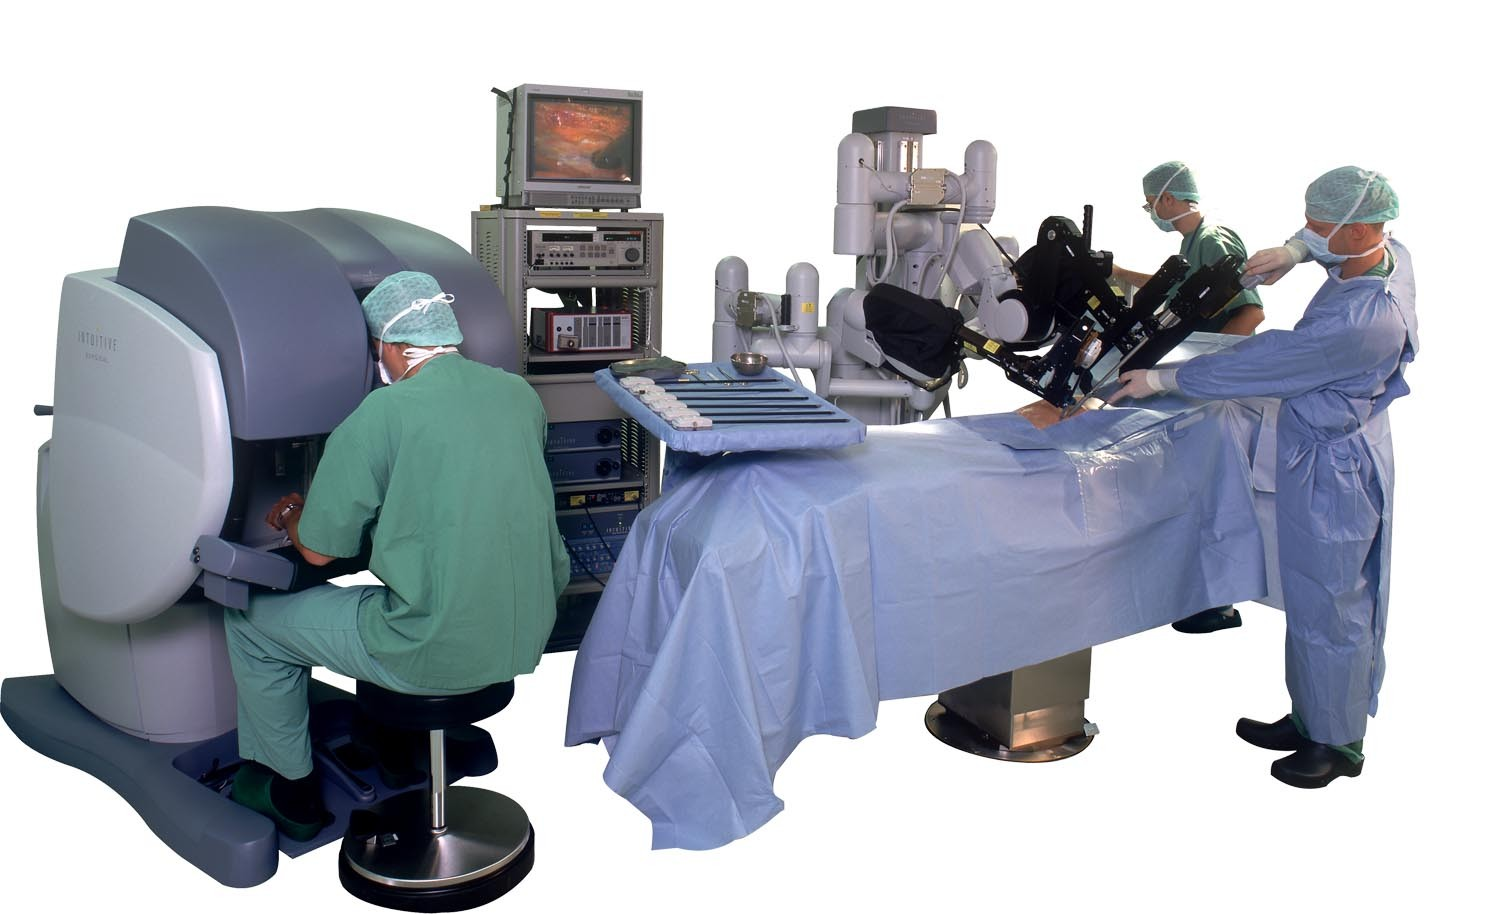
\includegraphics[width=1\textwidth]{Billeder/Dan/davinci.jpg}
	\end{figure}
\end{textblock*}

\end{frame}

\begin{frame}{Introduction}{Limitations of the da Vinci}<beamer>
\begin{itemize}
\item Surgeon has to estimate the force exerted by the tool
\item Studies show haptic feedback reduces error rate
\end{itemize}

\begin{textblock*}{0.7\textwidth}(4.5cm,3.5cm) % {block width} (coords)
  \begin{figure}[H]
  	\centering
  		\centering
  		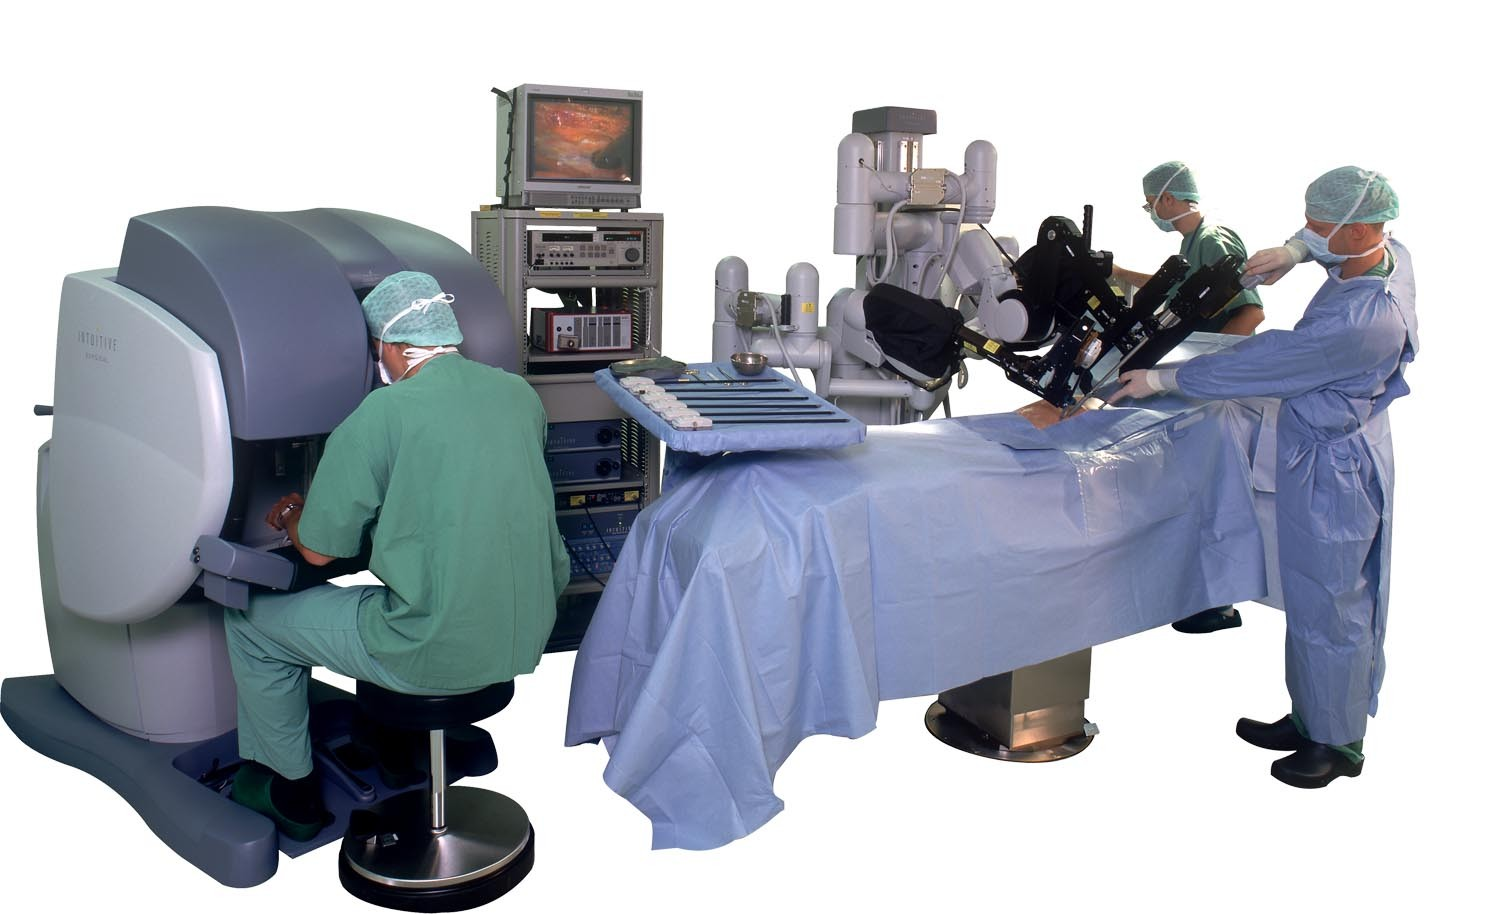
\includegraphics[width=1\textwidth]{Billeder/Dan/davinci.jpg}
  \end{figure}
\end{textblock*}

\end{frame}

\begin{frame}{Introduction}{Test setup}<beamer>
\begin{itemize}
\item Force feedback teleoperation of surgical tool
\item Geomagic Touch 
\begin{itemize}
\item 3 actuated degrees of freedom 
\item Cartesian force feedback
\item Outputs up to 3 N of force
\end{itemize}
\item EndoWrist
\begin{itemize}
	\item No force sensor
	\item High temperature sterilization
	\item Discarded after a couple of uses
\end{itemize}
\end{itemize}

\begin{figure}
	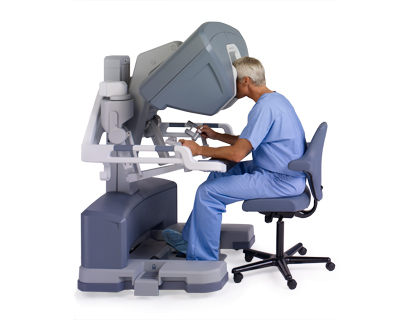
\includegraphics[width=0.3\textwidth]{Billeder/Dan/console.jpg}
	%\hspace{8mm}\vspace{-8mm} $\Rightarrow $ \vspace{8mm}\hspace{8mm}
	\resizebox{0.1\textwidth}{0.05\textwidth}{$\Rightarrow $}
	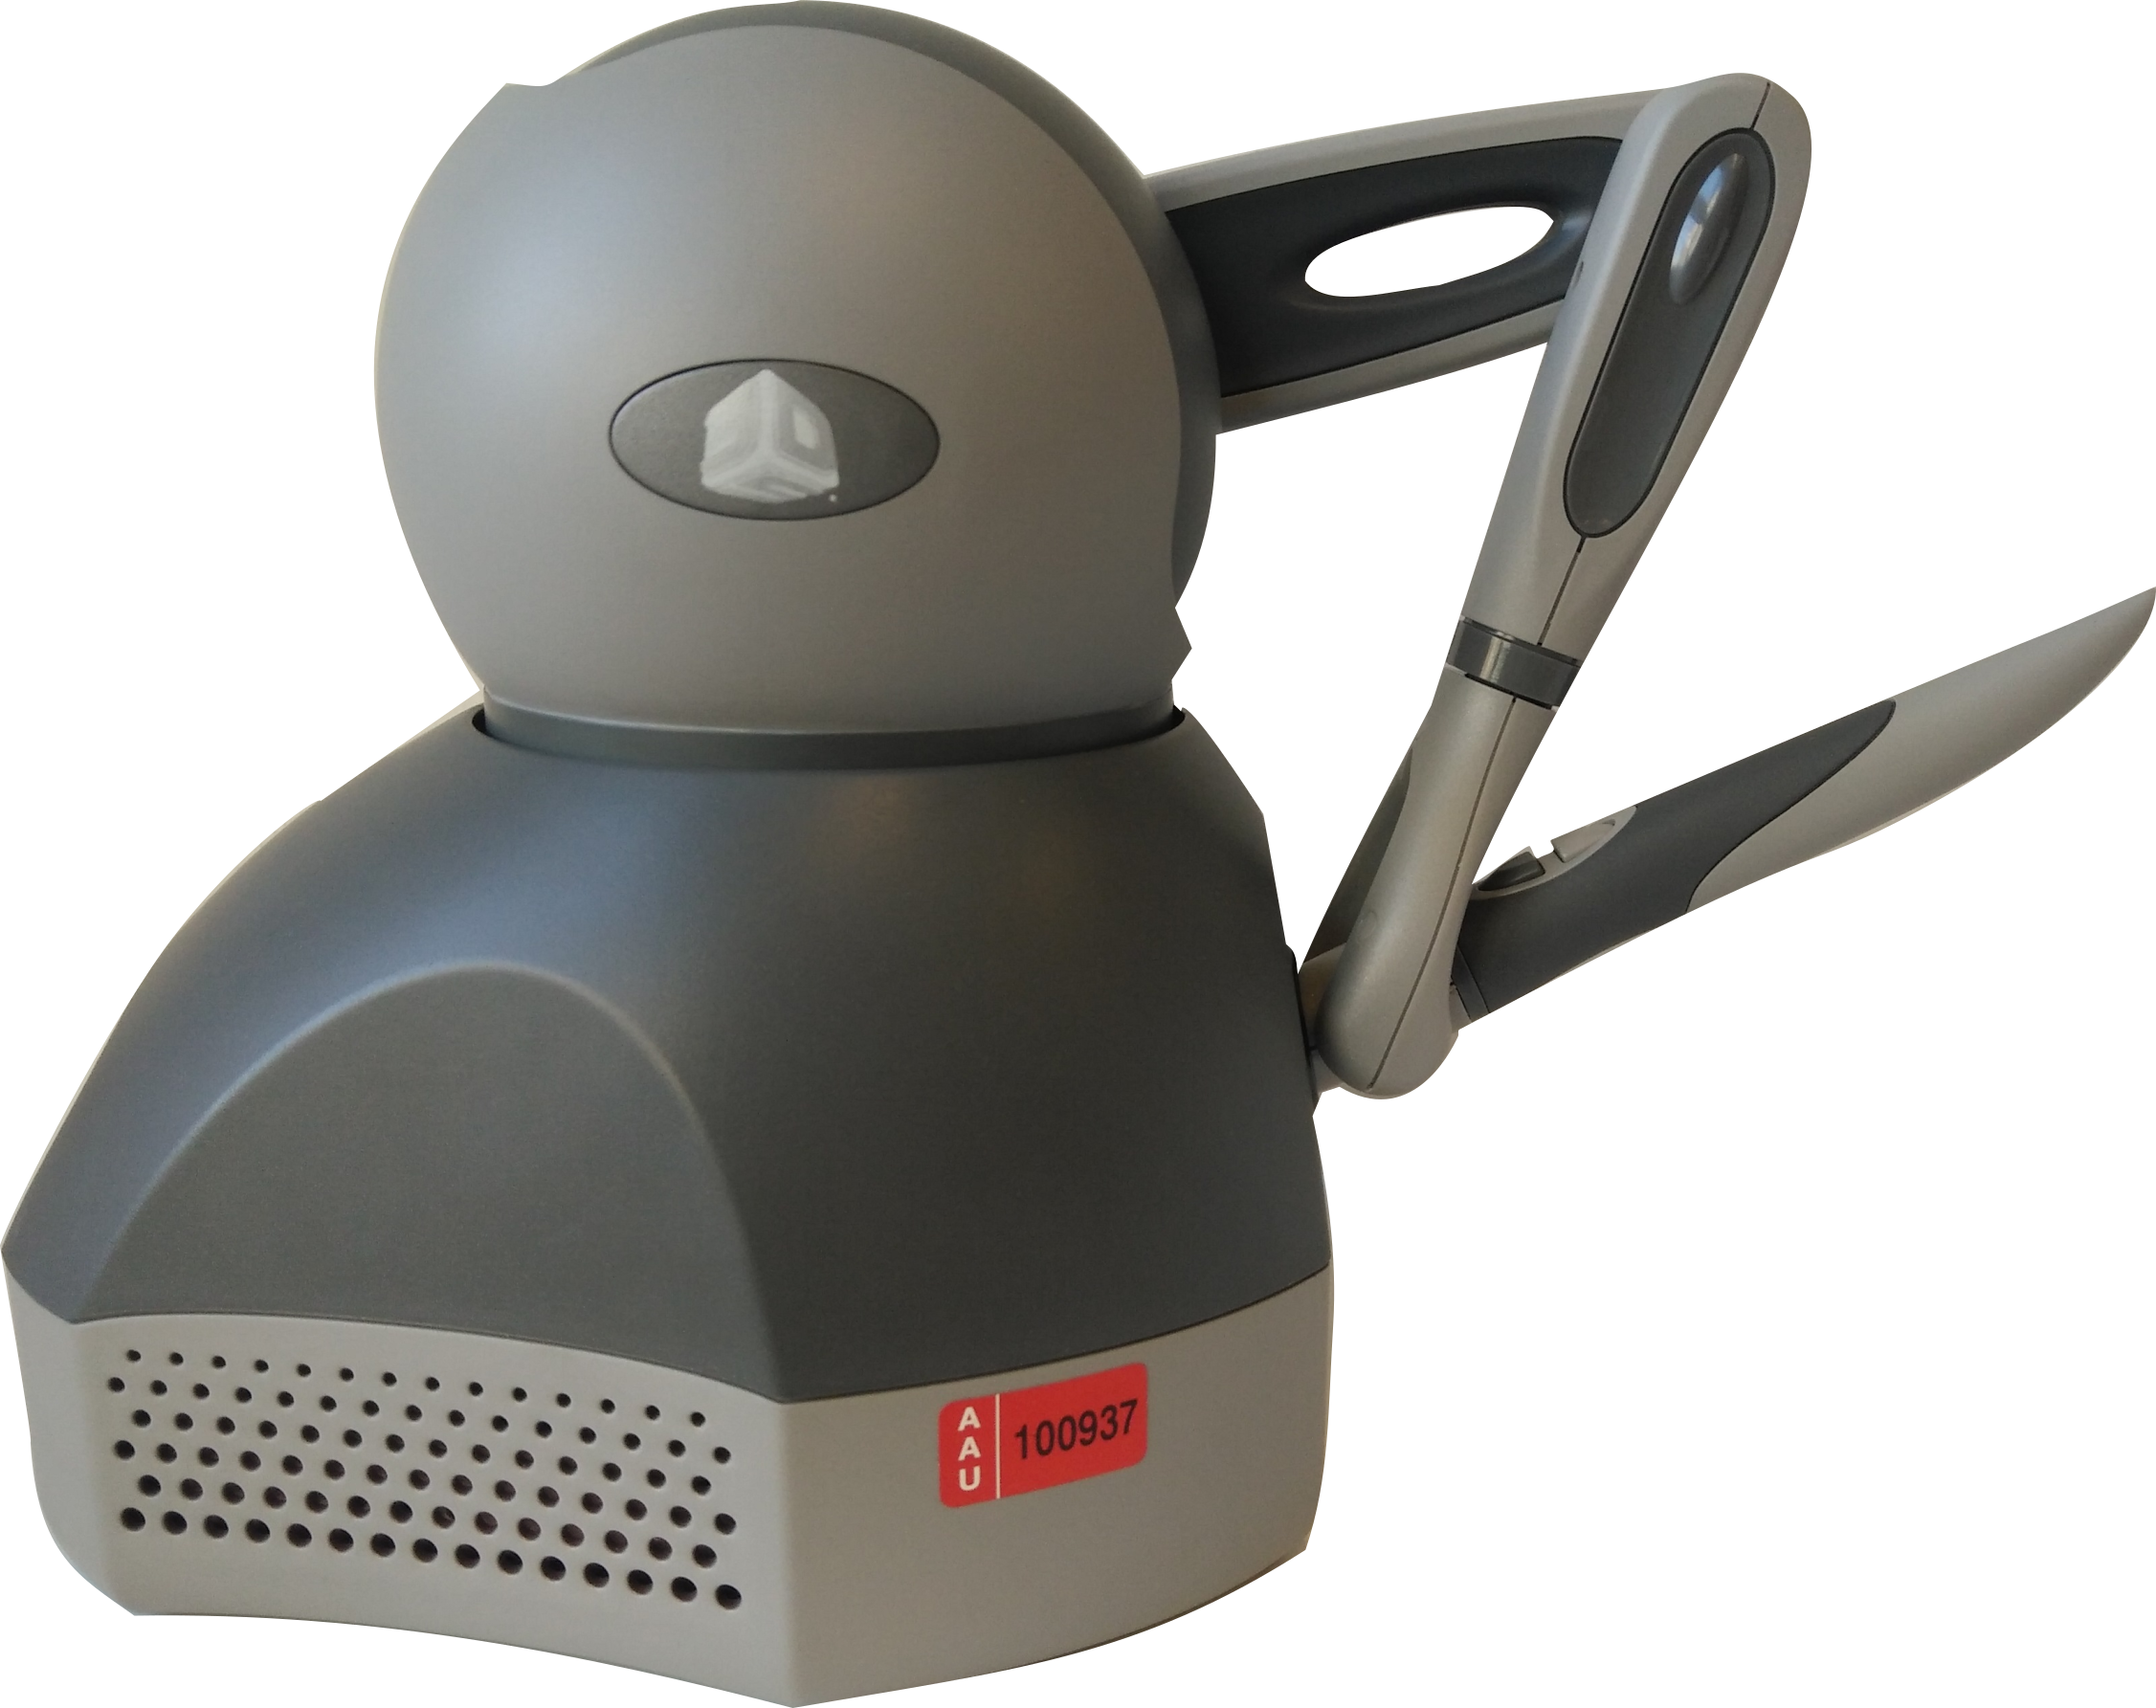
\includegraphics[width=0.3\textwidth]{Billeder/GT.png}
\end{figure}

\begin{textblock*}{0.7\textwidth}(8cm,3.5cm) % {block width} (coords)
	\begin{figure}[H]
		\centering
		\centering
		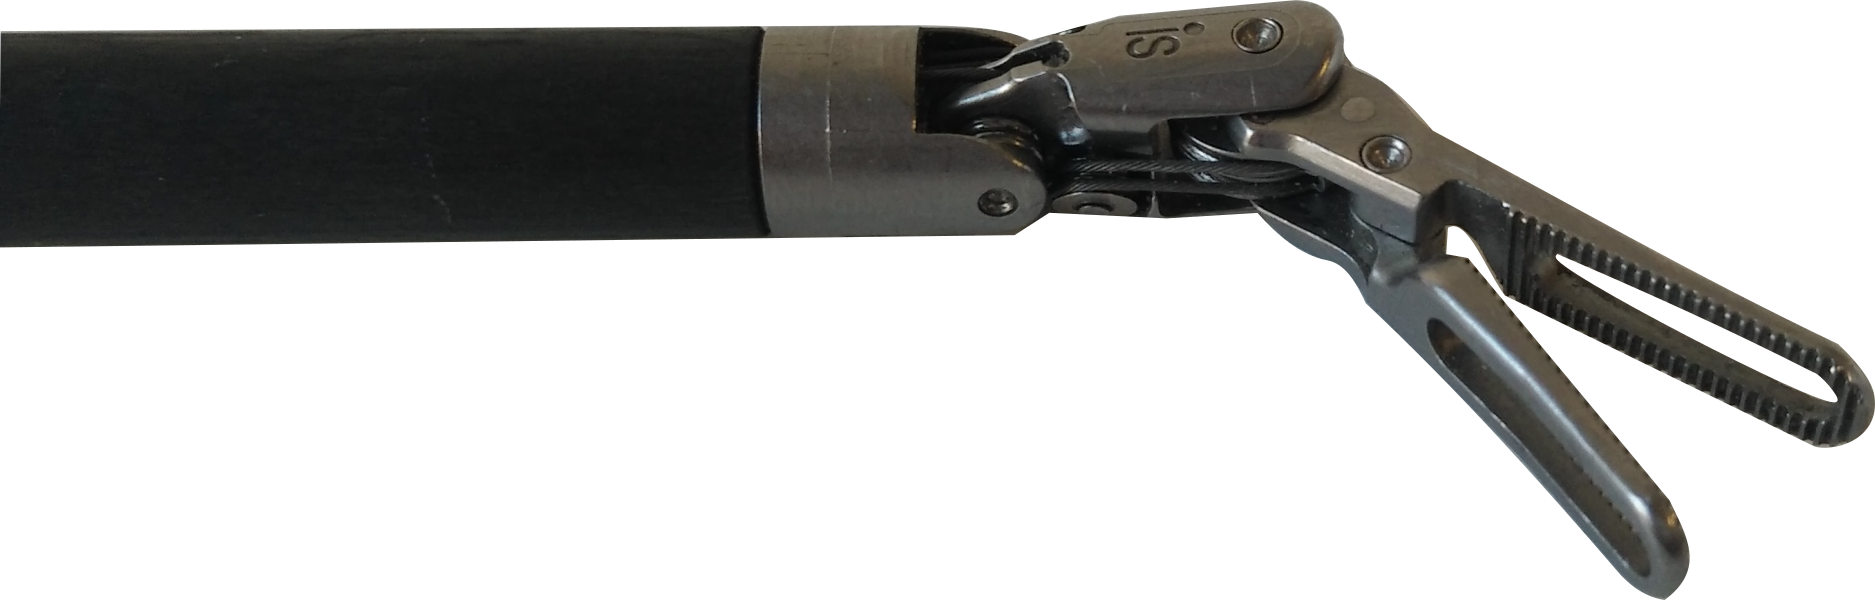
\includegraphics[width=0.4\textwidth]{Billeder/endo2.png}
	\end{figure}
\end{textblock*}


\end{frame}

\begin{frame}{Introduction}{Problem formulation}<beamer>
\begin{itemize}
\item Communication
\begin{itemize}
\item Minimize delays in communication
\end{itemize}
\item Force estimation
\begin{itemize}
\item Sensors too expensive for short lifetime of tools, EndoWrist dynamics have to be modelled
\end{itemize}
\item Control
\begin{itemize}
\item Remove oscillations in force feedback
\end{itemize}
\end{itemize}
\end{frame}
%%%%%%%%%%%%%%%%%%%%%%%%%%%%%%%%
\section{System overview}
%%%%%%%%%%%% MID WAY AGENDA %%%%%%%%%%%%%%
\begin{frame}<beamer>
\frametitle{System overview}
%\begin{figure}
%	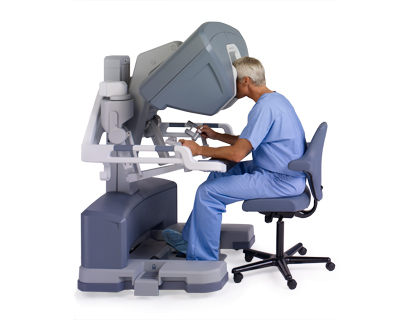
\includegraphics[width=0.2\textwidth]{Billeder/Dan/console.jpg}
%	\hspace{8mm}\vspace{-8mm} $\Rightarrow $ \vspace{8mm}\hspace{8mm}
%	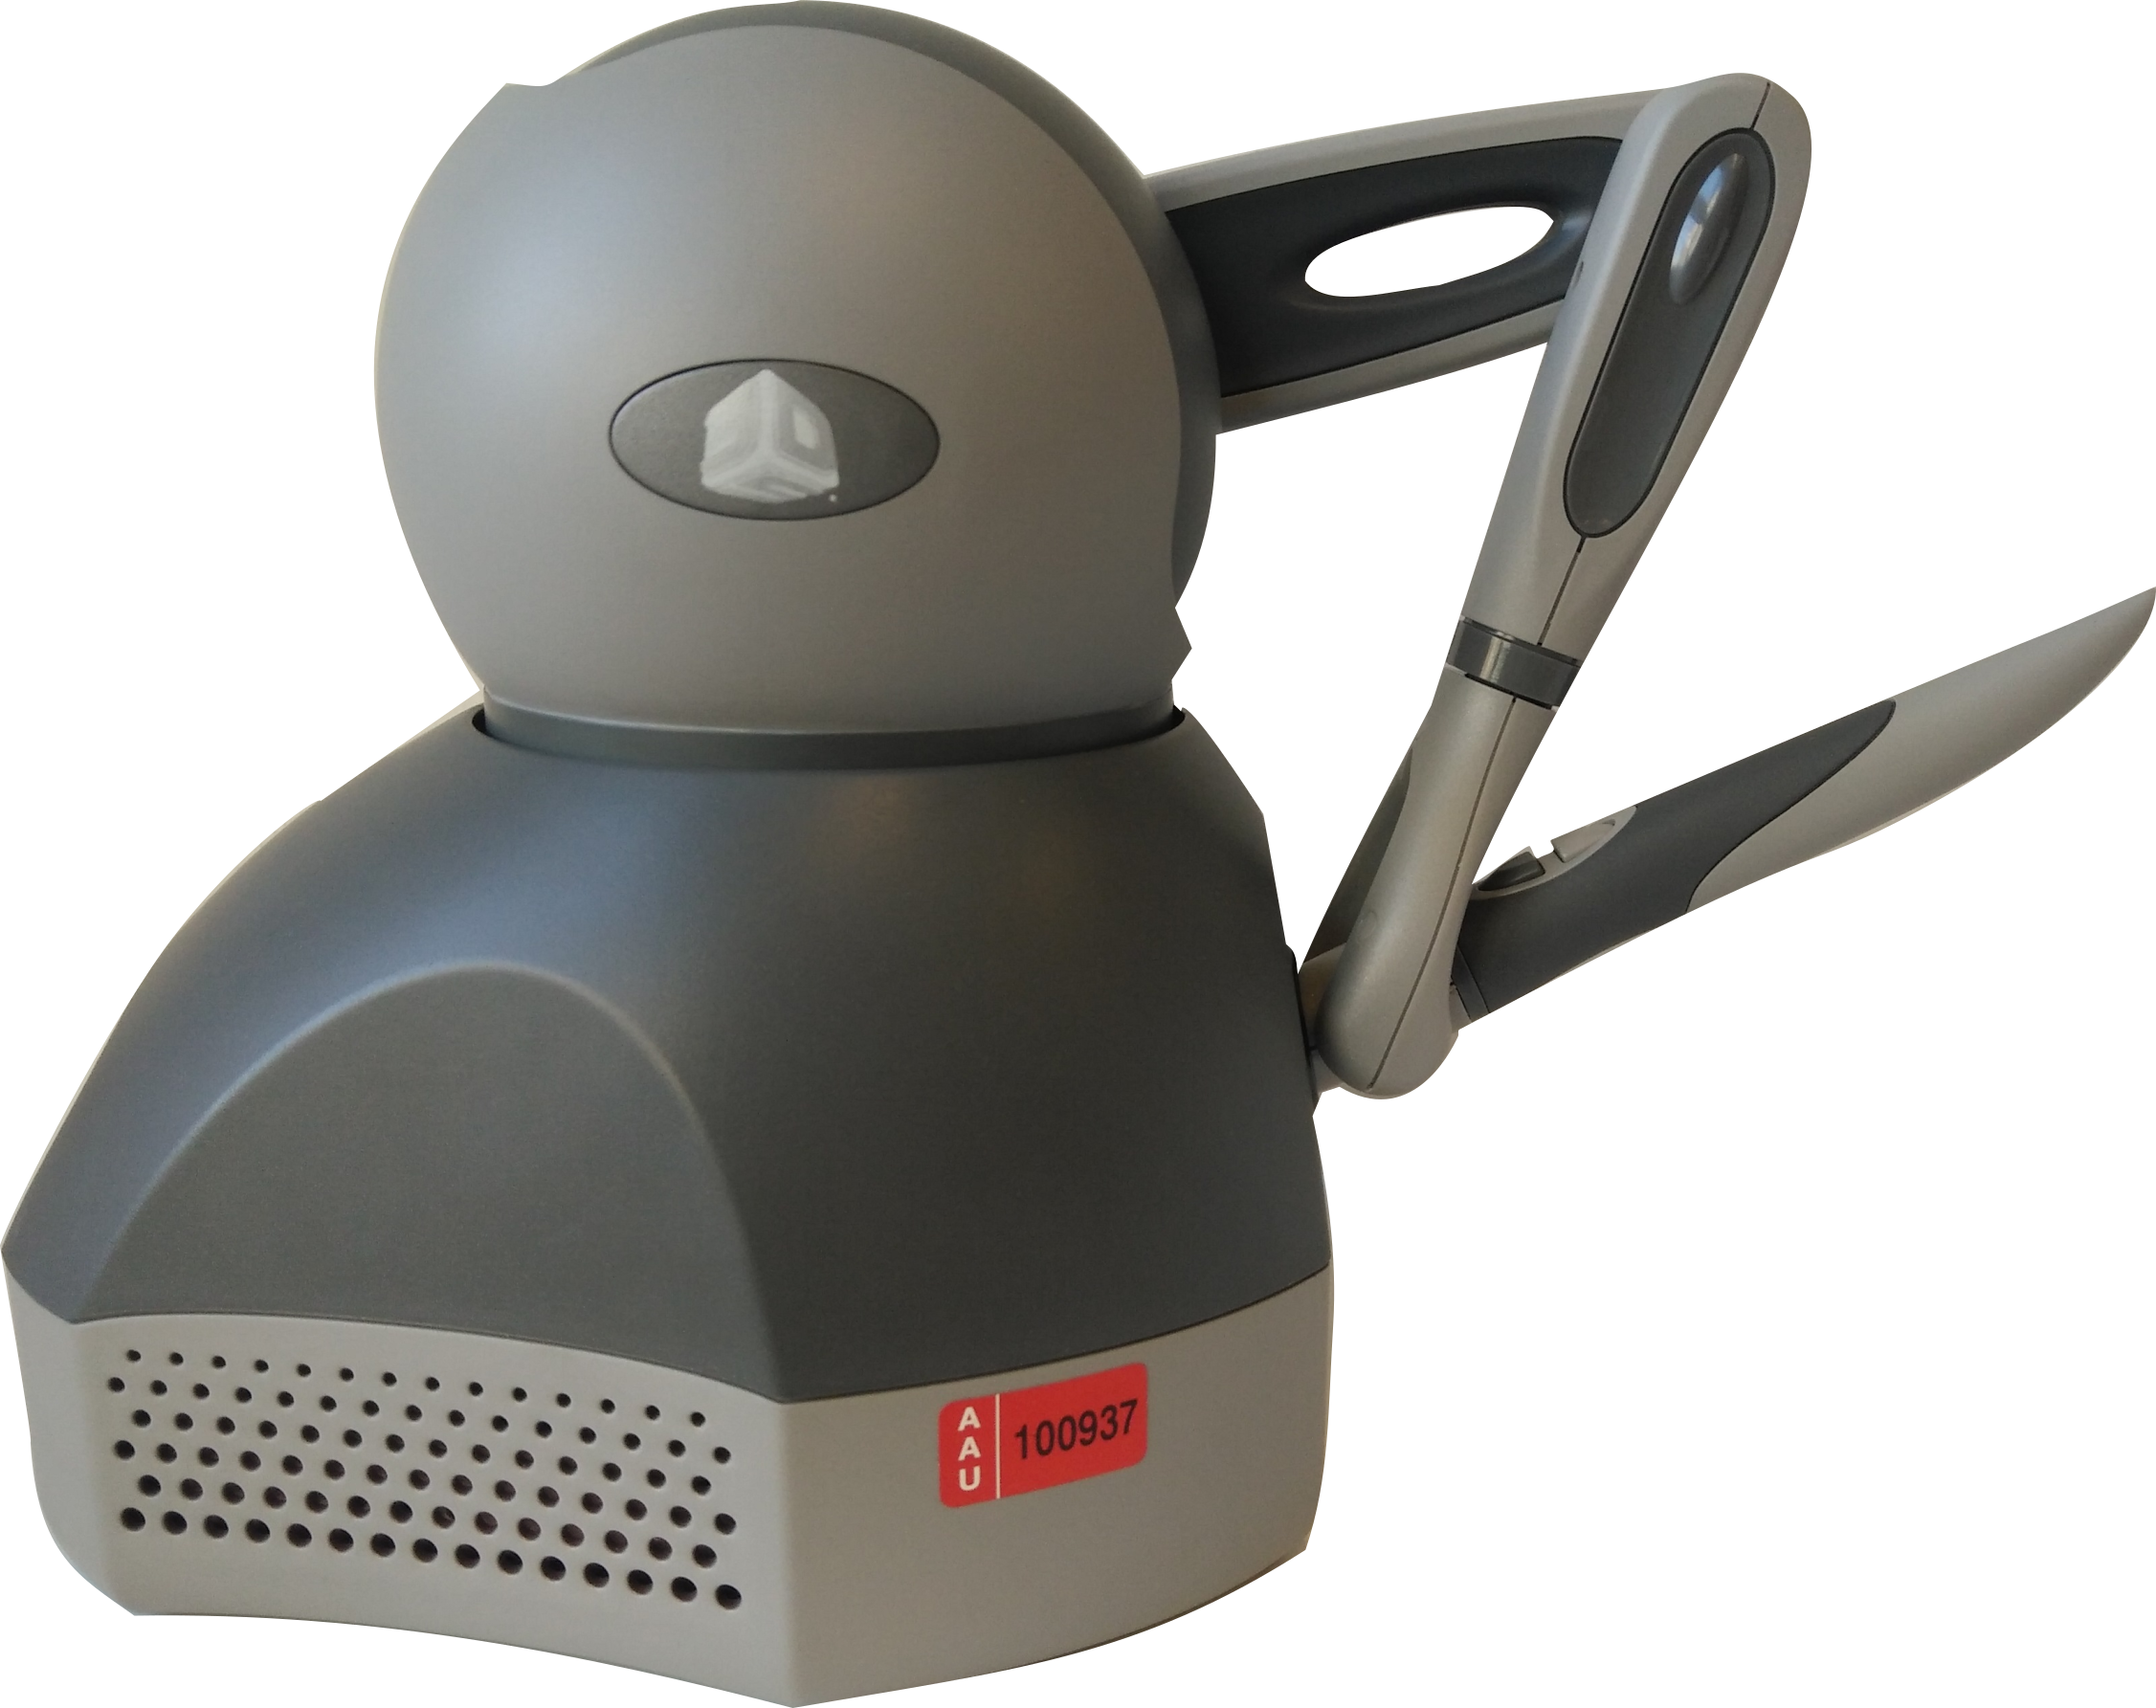
\includegraphics[width=0.2\textwidth]{Billeder/GT.png}
%\end{figure}

\begin{itemize}
	\item Operator controls the Geomagic Touch haptic device
	\item Control data is sent to a computer responsible for high level calculations
	\begin{itemize}
		\item Mapping
		\item Force estimation
	\end{itemize}
	\item sbRIO embedded system interfaces with motor controllers
	\item The motors move the EndoWrist using a custom made test equipment
\end{itemize}

\vspace{0.15\textheight}

\resizebox{\textwidth}{!}{
	\begin{tikzpicture}
	
	
	\node[box] (Opt) at (0,0) {Operator};
	\node[box] (Geo) at ($(3,0) + (Opt)$) {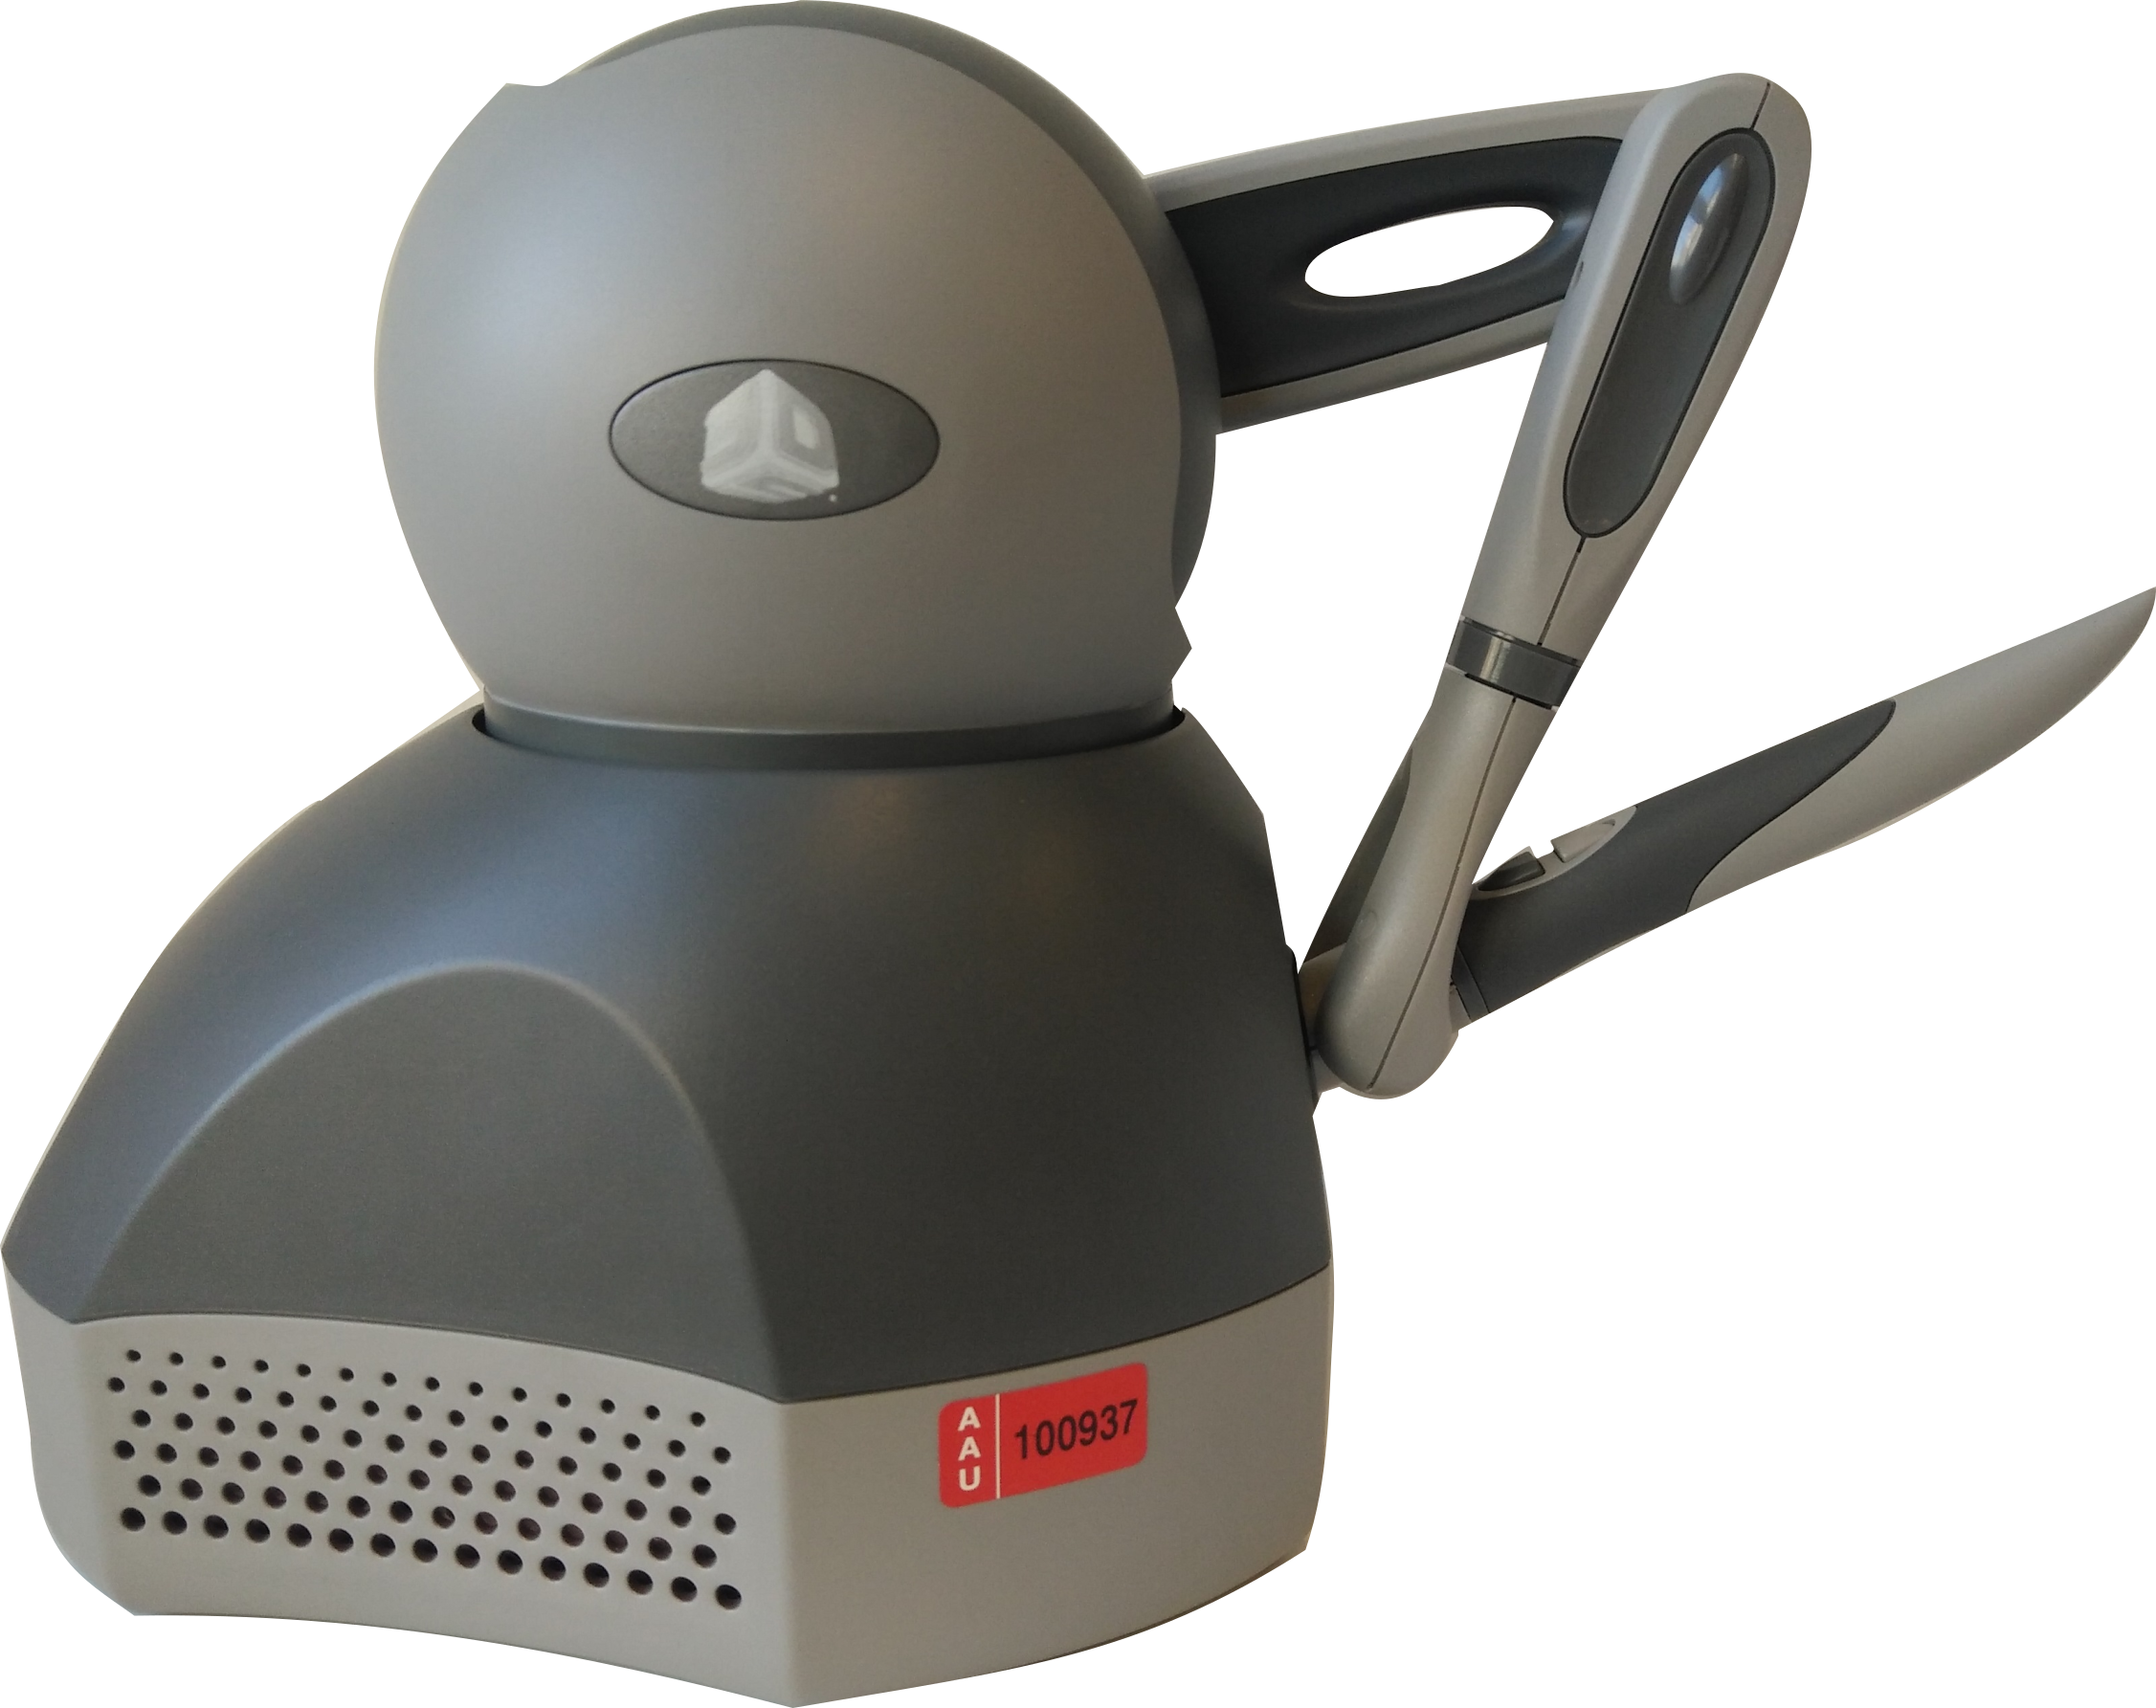
\includegraphics[width=0.2\textwidth]{Billeder/GT.png}};
	\node[box] (ros) at ($(3,0) + (Geo)$) {Computer};
	\node[box] (davin) at ($(3,0) + (ros)$) {\includegraphics[width=0.2\textwidth]{Billeder/Dan/sbRIO9636.png}};
	\node[box] (end) at ($(3,0) + (davin)$) {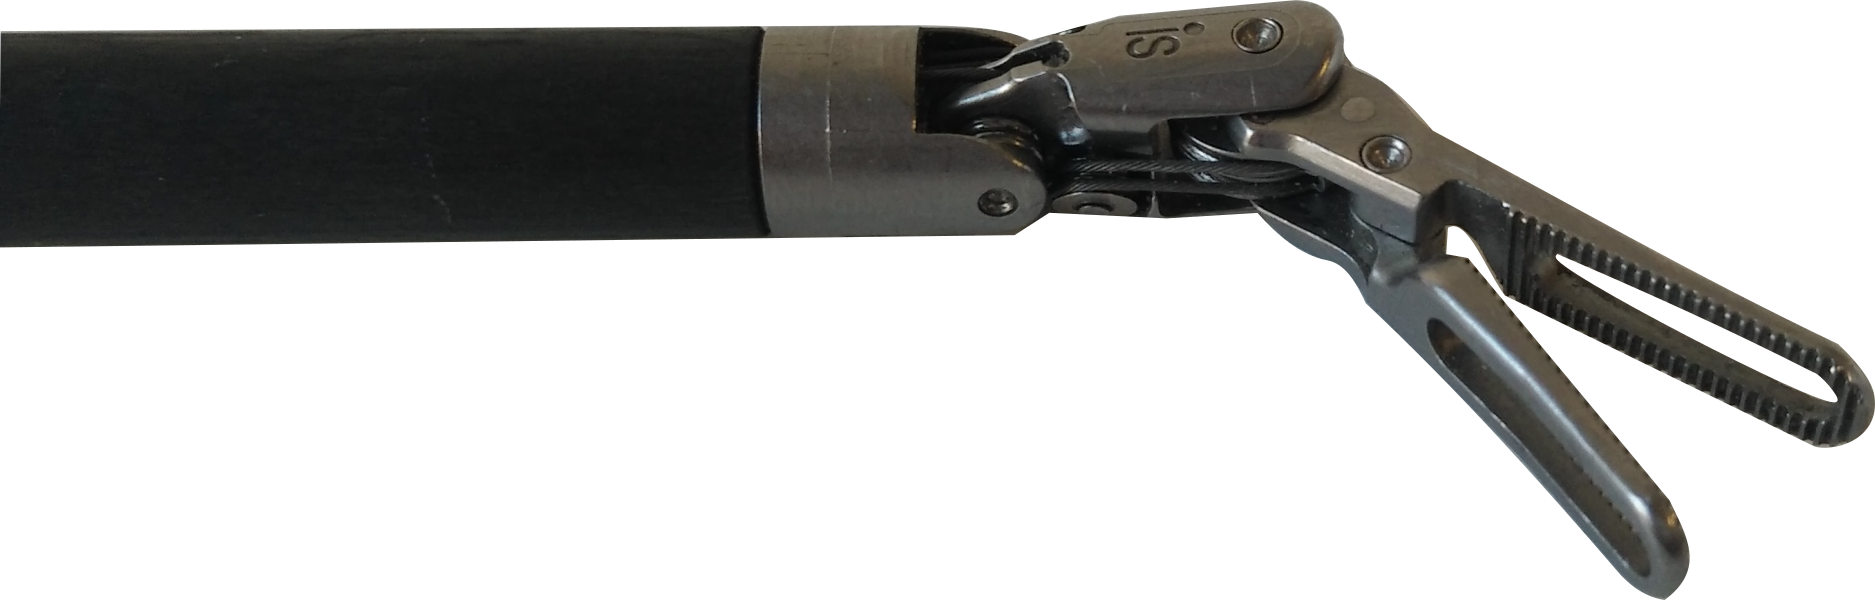
\includegraphics[width=0.2\textwidth]{Billeder/endo2.png}};
	
	
	\draw[->, ultra thick] ([yshift=0.3cm]Opt.east) -- ([yshift=0.3cm]Geo.west);
	\draw[->, ultra thick] ([yshift=0.3cm]Geo.east) -- ([yshift=0.3cm]ros.west);
	\draw[->, ultra thick] ([yshift=0.3cm]ros.east) -- ([yshift=0.3cm]davin.west);
	\draw[->, ultra thick] ([yshift=0.3cm]davin.east) -- ([yshift=0.3cm]end.west);
	
	
	\draw[<-, ultra thick] ([yshift=-0.3cm]Opt.east) -- ([yshift=-0.3cm]Geo.west);
	\draw[<-, ultra thick] ([yshift=-0.3cm]Geo.east) -- ([yshift=-0.3cm]ros.west);
	\draw[<-, ultra thick] ([yshift=-0.3cm]ros.east) -- ([yshift=-0.3cm]davin.west);
	%\draw[<-, ultra thick] ([yshift=-0.3cm]davin.east) -- ([yshift=-0.3cm]end.west);
	
	\node at (1.5,1.3) {Position};
	\node at (4.5,1.3) {Position};
	% \node at (7.5,1) {yes};
	% \node at (10.5,1) {yes};
	
	\node at (1.5,-1.3) {Force};
	\node at (4.5,-1.3) {Force};
	\node at (10.5,1.3) {Torque};
	% \node at (10.5,1) {yes};
	%\node at (7.5,1.5) {Motor enable};
	\node at (7.5,1.3) {Position};
	\node at (7.5,-1.3) {Position};
	\node at (7.5,-1.8) {Velocity};
	\node at (7.5,-2.3) {Current};
	
	\end{tikzpicture}
}
\end{frame}
%%%%%%%%%%%%%%%%%%%%%%%%%%%%%%%%
\section{Communication}
%%%%%%%%%%%% MID WAY AGENDA %%%%%%%%%%%%%%
\begin{frame}<beamer>
\frametitle{Communication overview}
  \begin{figure}
  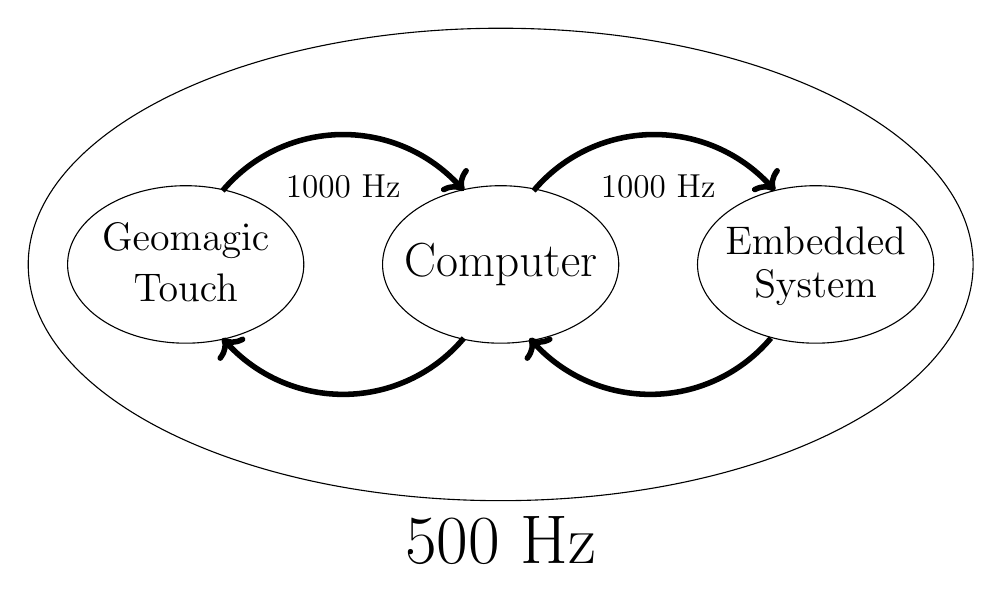
\begin{tikzpicture}

  \draw  (-3,0) ellipse (1.5 and 1)node (v1) {\LARGE Computer};
  \draw  (-7,0) ellipse (1.5 and 1)node{};
  \draw  (1,0) ellipse (1.5 and 1)node{};
  \node at (1,0.3) {\Large Embedded};
  \node at (1,-0.3) {\Large System};
  \node at (-7,0.3) {\Large Geomagic};
  \node at (-7,-0.3) {\Large Touch};

  \draw [->,line width=2pt](-6.5321,0.9356) arc (139.9997:40:2);
  \draw [<-,line width=2pt](-6.5321,-0.9356) arc (-139.9997:-40:2);
  \draw [<-,line width=2pt](-2.6321,-0.9356) arc (-139.9997:-40:2);
  \draw [->,line width=2pt](-2.5821,0.9356) arc (139.9997:40:2);


  \node at (-5,1) {\large 1000 Hz};
  \node at (-1,1) {\large 1000 Hz};
  \draw  (v1) ellipse (6 and 3);
  \node at (-3,-3.5) {\Huge 500 Hz};
  \end{tikzpicture}
  \end{figure}
\end{frame}

% the license
\begin{frame}<beamer>
\frametitle{Communication}


  \begin{itemize}
  \item<1-> Maximum for the initial system: 100 Hz
  \item<1-> Our approach:
      \begin{itemize}
        \item<1-> Reducing the size of exchanged data
        \item<1-> Changing the transport protocol
      \end{itemize}
  \end{itemize}
\end{frame}

\begin{frame}<beamer>
\frametitle{Reducing the size of the packet}
\begin{figure}[h]
\centering
\begin{minipage}{.45\textwidth}
\resizebox{\textwidth}{!}{
  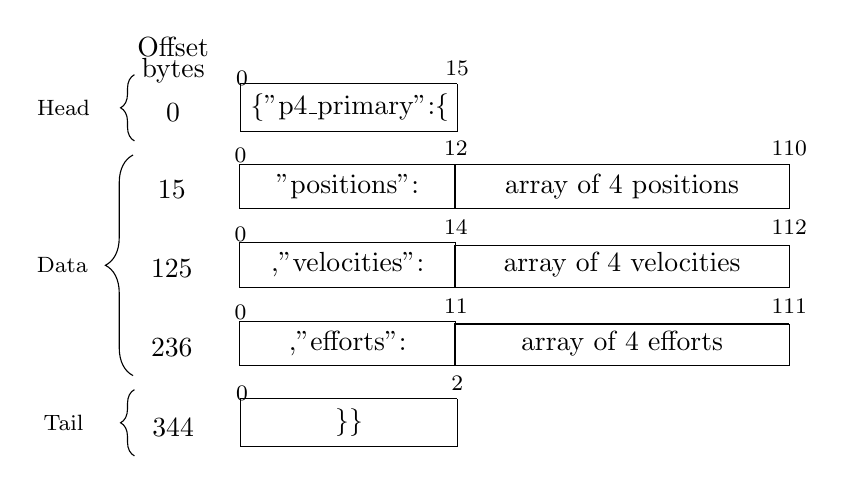
\begin{tikzpicture}
      \matrix(dict1)[matrix of nodes,ampersand replacement=\&, %below=of game,
          nodes={align=center,text width=2.5cm},
          row 1/.style={anchor=south},
          column 1/.style={nodes={text width = 1.5cm}}
      ]{
      0   \& \{"p4\_primary":\{\\
      };


      \matrix(dict2)[matrix of nodes,ampersand replacement=\&,%below=of game,
          nodes={align=center,text width=2.5cm},
          row 1/.style={anchor=south},
          column 1/.style={nodes={text width = 1.5cm}},
          column 3/.style={nodes={text width = 4cm}}
      ] at ($(dict1)+ (2.1,-1)$){
      15  \& "positions": \& array of 4 positions\\
      };

      \matrix(dict3)[matrix of nodes,ampersand replacement=\&,%below=of game,
          nodes={align=center,text width=2.5cm},
          row 1/.style={anchor=south},
          column 1/.style={nodes={text width = 1.5cm}},
          column 3/.style={nodes={text width = 4cm}}
      ] at ($(dict2)+ (0,-1)$){
      125 \& ,"velocities": \& array of 4 velocities\\
      };

      \matrix(dict4)[matrix of nodes,ampersand replacement=\&,%below=of game,
          nodes={align=center,text width=2.5cm},
          row 1/.style={anchor=south},
          column 1/.style={nodes={text width = 1.5cm}},
          column 3/.style={nodes={text width = 4cm}}
      ] at ($(dict3)+ (0,-1)$){
      236 \& ,"efforts": \& array of 4 efforts\\
      };

      \matrix(dict5)[matrix of nodes,ampersand replacement=\&,%below=of game,
          nodes={align=center,text width=2.5cm},
          row 1/.style={anchor=south},
          column 1/.style={nodes={text width = 1.5cm}}
      ] at ($(dict4)+ (-2.1,-1)$){
      344 \& \}\} \\
      };

  %Boxes
      \draw(dict1-1-2.north east)--(dict1-1-2.north west)--(dict1-1-2.south west)--(dict1-1-2.south east)--(dict1-1-2.north east);
      \draw(dict2-1-2.north east)--(dict2-1-2.north west)--(dict2-1-2.south west)--(dict2-1-2.south east)--(dict2-1-2.north east);
      \draw(dict3-1-2.north east)--(dict3-1-2.north west)--(dict3-1-2.south west)--(dict3-1-2.south east)--(dict3-1-2.north east);
      \draw(dict4-1-2.north east)--(dict4-1-2.north west)--(dict4-1-2.south west)--(dict4-1-2.south east)--(dict4-1-2.north east);
      \draw(dict5-1-2.north east)--(dict5-1-2.north west)--(dict5-1-2.south west)--(dict5-1-2.south east)--(dict5-1-2.north east);


      \draw(dict2-1-3.north east)--(dict2-1-3.north west)--(dict2-1-3.south west)--(dict2-1-3.south east)--(dict2-1-3.north east);
      \draw($(dict3-1-3.north east)+(0,-0.03)$)--($(dict3-1-3.north west)+(0,-0.03)$)--(dict3-1-3.south west)--(dict3-1-3.south east)--($(dict3-1-3.north east)+(0,-0.03)$);
      \draw($(dict4-1-3.north east)+(0,-0.03)$)--($(dict4-1-3.north west)+(0,-0.03)$)--(dict4-1-3.south west)--(dict4-1-3.south east)--($(dict4-1-3.north east)+(0,-0.03)$);

  %curly braces
    \draw [decorate,decoration={brace,amplitude=10pt, mirror},xshift=-4pt,yshift=0pt]
    ($(dict2.north west)+(0.5,0)$) -- ($(dict4.south west)+(0.5,0)$) node [black,midway,xshift=-0.9cm] {\footnotesize Data};

    \draw [decorate,decoration={brace,amplitude=5pt, mirror},xshift=-4pt,yshift=0pt]
    ($(dict1.north west)+(0.5,0)$) -- ($(dict1.south west)+(0.5,0)$) node [black,midway,xshift=-0.9cm] {\footnotesize Head};

    \draw [decorate,decoration={brace,amplitude=5pt, mirror},xshift=-4pt,yshift=0pt]
    ($(dict5.north west)+(0.5,0)$) -- ($(dict5.south west)+(0.5,0)$) node [black,midway,xshift=-0.9cm] {\footnotesize Tail};

  %numbers
    \node at ($(dict1-1-1.north east)+(0,0.2)$) {\footnotesize 0};
    \node at ($(dict1-1-2.north east)+(0,0.2)$) {\footnotesize 15};

    \node at ($(dict2-1-1.north east)+(0,0.2)$) {\footnotesize 0};
    \node at ($(dict2-1-2.north east)+(0,0.2)$) {\footnotesize 12};
    \node at ($(dict2-1-3.north east)+(0,0.2)$) {\footnotesize 110};

    \node at ($(dict3-1-1.north east)+(0,0.2)$) {\footnotesize 0};
    \node at ($(dict3-1-2.north east)+(0,0.2)$) {\footnotesize 14};
    \node at ($(dict3-1-3.north east)+(0,0.2)$) {\footnotesize 112};

    \node at ($(dict4-1-1.north east)+(0,0.2)$) {\footnotesize 0};
    \node at ($(dict4-1-2.north east)+(0,0.2)$) {\footnotesize 11};
    \node at ($(dict4-1-3.north east)+(0,0.2)$) {\footnotesize 111};

    \node at ($(dict5-1-1.north east)+(0,0.2)$) {\footnotesize 0};
    \node at ($(dict5-1-2.north east)+(0,0.2)$) {\footnotesize 2};

      \node at ($(0,0.3)+(dict1-1-1.north)$) {bytes};
      \node at ($(0,0.6)+(dict1-1-1.north)$) {Offset};

  \end{tikzpicture}
  }
  \caption{Packet built using JSON}
  \label{fig:old_packets}
\end{minipage}
\begin{minipage}{.45\textwidth}
\centering
\resizebox{\textwidth}{!}{
  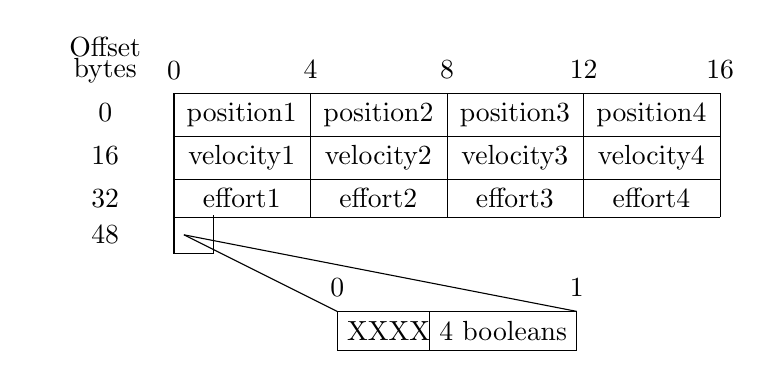
\begin{tikzpicture}
      \matrix(dict)[matrix of nodes,ampersand replacement=\&, %below=of game,
          nodes={align=center,text width=1.5cm},
          row 1/.style={anchor=south}%,
          column 1/.style={nodes={text width = 0.5cm, align=right}}
      ]{
      0   \& position1 \& position2 \& position3 \& position4\\
      16  \& velocity1 \& velocity2 \& velocity3 \& velocity4\\
      32  \& effort1   \& effort2   \& effort3   \& effort4\\
      48  \\
      };
      %horizontal
      \draw(dict-1-2.north west)--(dict-1-5.north east);
      \draw(dict-1-2.south west)--(dict-1-5.south east);
      \draw(dict-2-2.south west)--(dict-2-5.south east);
      \draw(dict-3-2.south west)--(dict-3-5.south east);
    %vertical
      \draw(dict-1-1.north east)--(dict-4-1.south east);
      \draw(dict-1-2.north east)--(dict-3-2.south east);
      \draw(dict-1-3.north east)--(dict-3-3.south east);
      \draw(dict-1-4.north east)--(dict-3-4.south east);
      \draw(dict-1-5.north east)--(dict-3-5.south east);

      %small at bottom
      \draw(dict-4-1.south east)--($(0.5,0)+(dict-4-1.south east)$);
      \draw($(0.5,0)+(dict-4-1.south east)$)--($(0.5,0.49)+(dict-4-1.south east)$);

      %numbers on top
      \node at ($(0,0.3)+(dict-1-1.north east)$) {0};
      \node at ($(0,0.3)+(dict-1-2.north east)$) {4};
      \node at ($(0,0.3)+(dict-1-3.north east)$) {8};
      \node at ($(0,0.3)+(dict-1-4.north east)$) {12};
      \node at ($(0,0.3)+(dict-1-5.north east)$) {16};

      \node at ($(0,0.3)+(dict-1-1.north)$) {bytes};
      \node at ($(0,0.6)+(dict-1-1.north)$) {Offset};

      %The zoom on the last byte
      \node (zoom) at (1,-2) {XXXX 4 booleans};
      \draw(zoom.north east)--(zoom.north west);
      \draw(zoom.north east)--(zoom.south east);
      \draw(zoom.north west)--(zoom.south west);
      \draw(zoom.south east)--(zoom.south west);
      \draw($(zoom.north)+(-0.35,0)$)--($(zoom.south)+(-0.35,0)$);
      \draw(zoom.north east)--($(1,0)+(dict-4-1)$);
      \draw(zoom.north west)--($(1,0)+(dict-4-1)$);
      \node at ($(zoom.north east)+(0,0.3)$) {1};
      \node at ($(zoom.north west)+(0,0.3)$) {0};

  \end{tikzpicture}
  }
  \caption{Packet built using the binary representation}
  \label{fig:new_packets}
\end{minipage}
\end{figure}
\begin{center}
  Size reduced by 85\%
  \end{center}
\end{frame}


\begin{frame}<beamer>
\frametitle{Communication}
\begin{itemize}
	\item Changed from TCP/IP to UDP
	\begin{itemize}
	\item Less overhead
	\end{itemize}
    \item Results: maximum of 638 Hz
\end{itemize}
\end{frame}



% \begin{frame}<beamer>
% \frametitle{Friction model}
%   \begin{figure}[h]
% \centering
%   \begin{tikzpicture}
%   %axes
%   \draw [->,thick] (-3,0) -- (3,0);
%   \draw [->,thick] (0,-2.2) -- (0,2.2);
%   %model
%   \draw [ultra thick, color=blue] (0,-1.6) -- (0,1.6);
%   \draw [ultra thick, color=blue] (0,1.6) -- (3,1.6);
%   \draw [ultra thick, color=blue] (0,-1.6) -- (-3,-1.6);
%   %name of axis and variables
%   \node at (-0.4,1.6) {$\tau_s$};
%   \draw (-0.22,1.6) -- (-0.1,1.6);

%   \node at (3,0.4) {$\omega$};
%   \node at (0.4,2.2) {$\tau_f$};

%   \end{tikzpicture}
% \caption{final friction model}
% \label{fig:new_friction_model}
% \end{figure}
% \end{frame}

%%%%%%%%%%%%%%%%%%%%%%%%%%%%%%%%
\section{Force estimation}
%%%%%%%%%%%% MID WAY AGENDA %%%%%%%%%%%%%%
\begin{frame}{Force estimation}
\end{frame}

\begin{frame}{Force estimation}{Overview}
\begin{itemize}
\item Elasticity and friction between wires cause nonlinearities in the EndoWristis dynamics
\item Model available, derived using large scale replica of mechanism
	\begin{itemize}
		\item Unable to fit model to data gathered with our setup
	\end{itemize}
	
\item Model with defined general structure fitted to gathered data
	\begin{itemize}
		\item Black-box identification
	\end{itemize}

\item Model correction
	\begin{itemize}
		\item Can we use measurable quantities to correct the force estimate?
	\end{itemize}

\end{itemize}
\end{frame}

\begin{frame}{Force estimation}{Overview}
\begin{itemize}
  	\item Roll, pitch and yaw forces
\end{itemize}
 \begin{figure}[h]
 \centering
 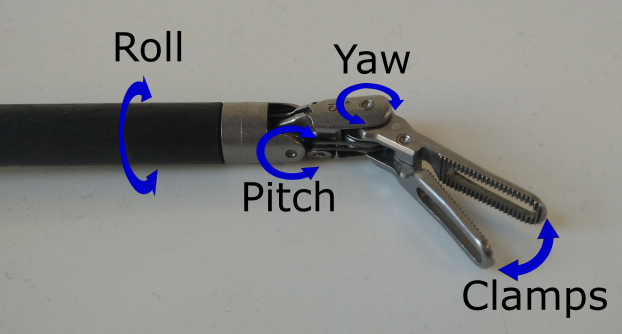
\includegraphics[scale = 0.5]{Endowrist31}
 \label{fig:ewr}
 \end{figure}
\end{frame}

\begin{frame}{Force estimation}{Data acquisition}
\begin{itemize}
\item Roll torque measurement made with torque sensor
\item Yaw and Pitch force measurement made with load cell setup
\begin{itemize}
\item Load cell output read by Arduino logged by sbRIO
\item Position, velocity, current (effort) and setpoints logged by sbRIO
\end{itemize}
\item Measurement process slow and prone to error
\begin{itemize}
\item Disturbances in data
\end{itemize}
\end{itemize}
\begin{figure}
\centering
    \begin{subfigure}[t]{0.32\textwidth}
        \centering
        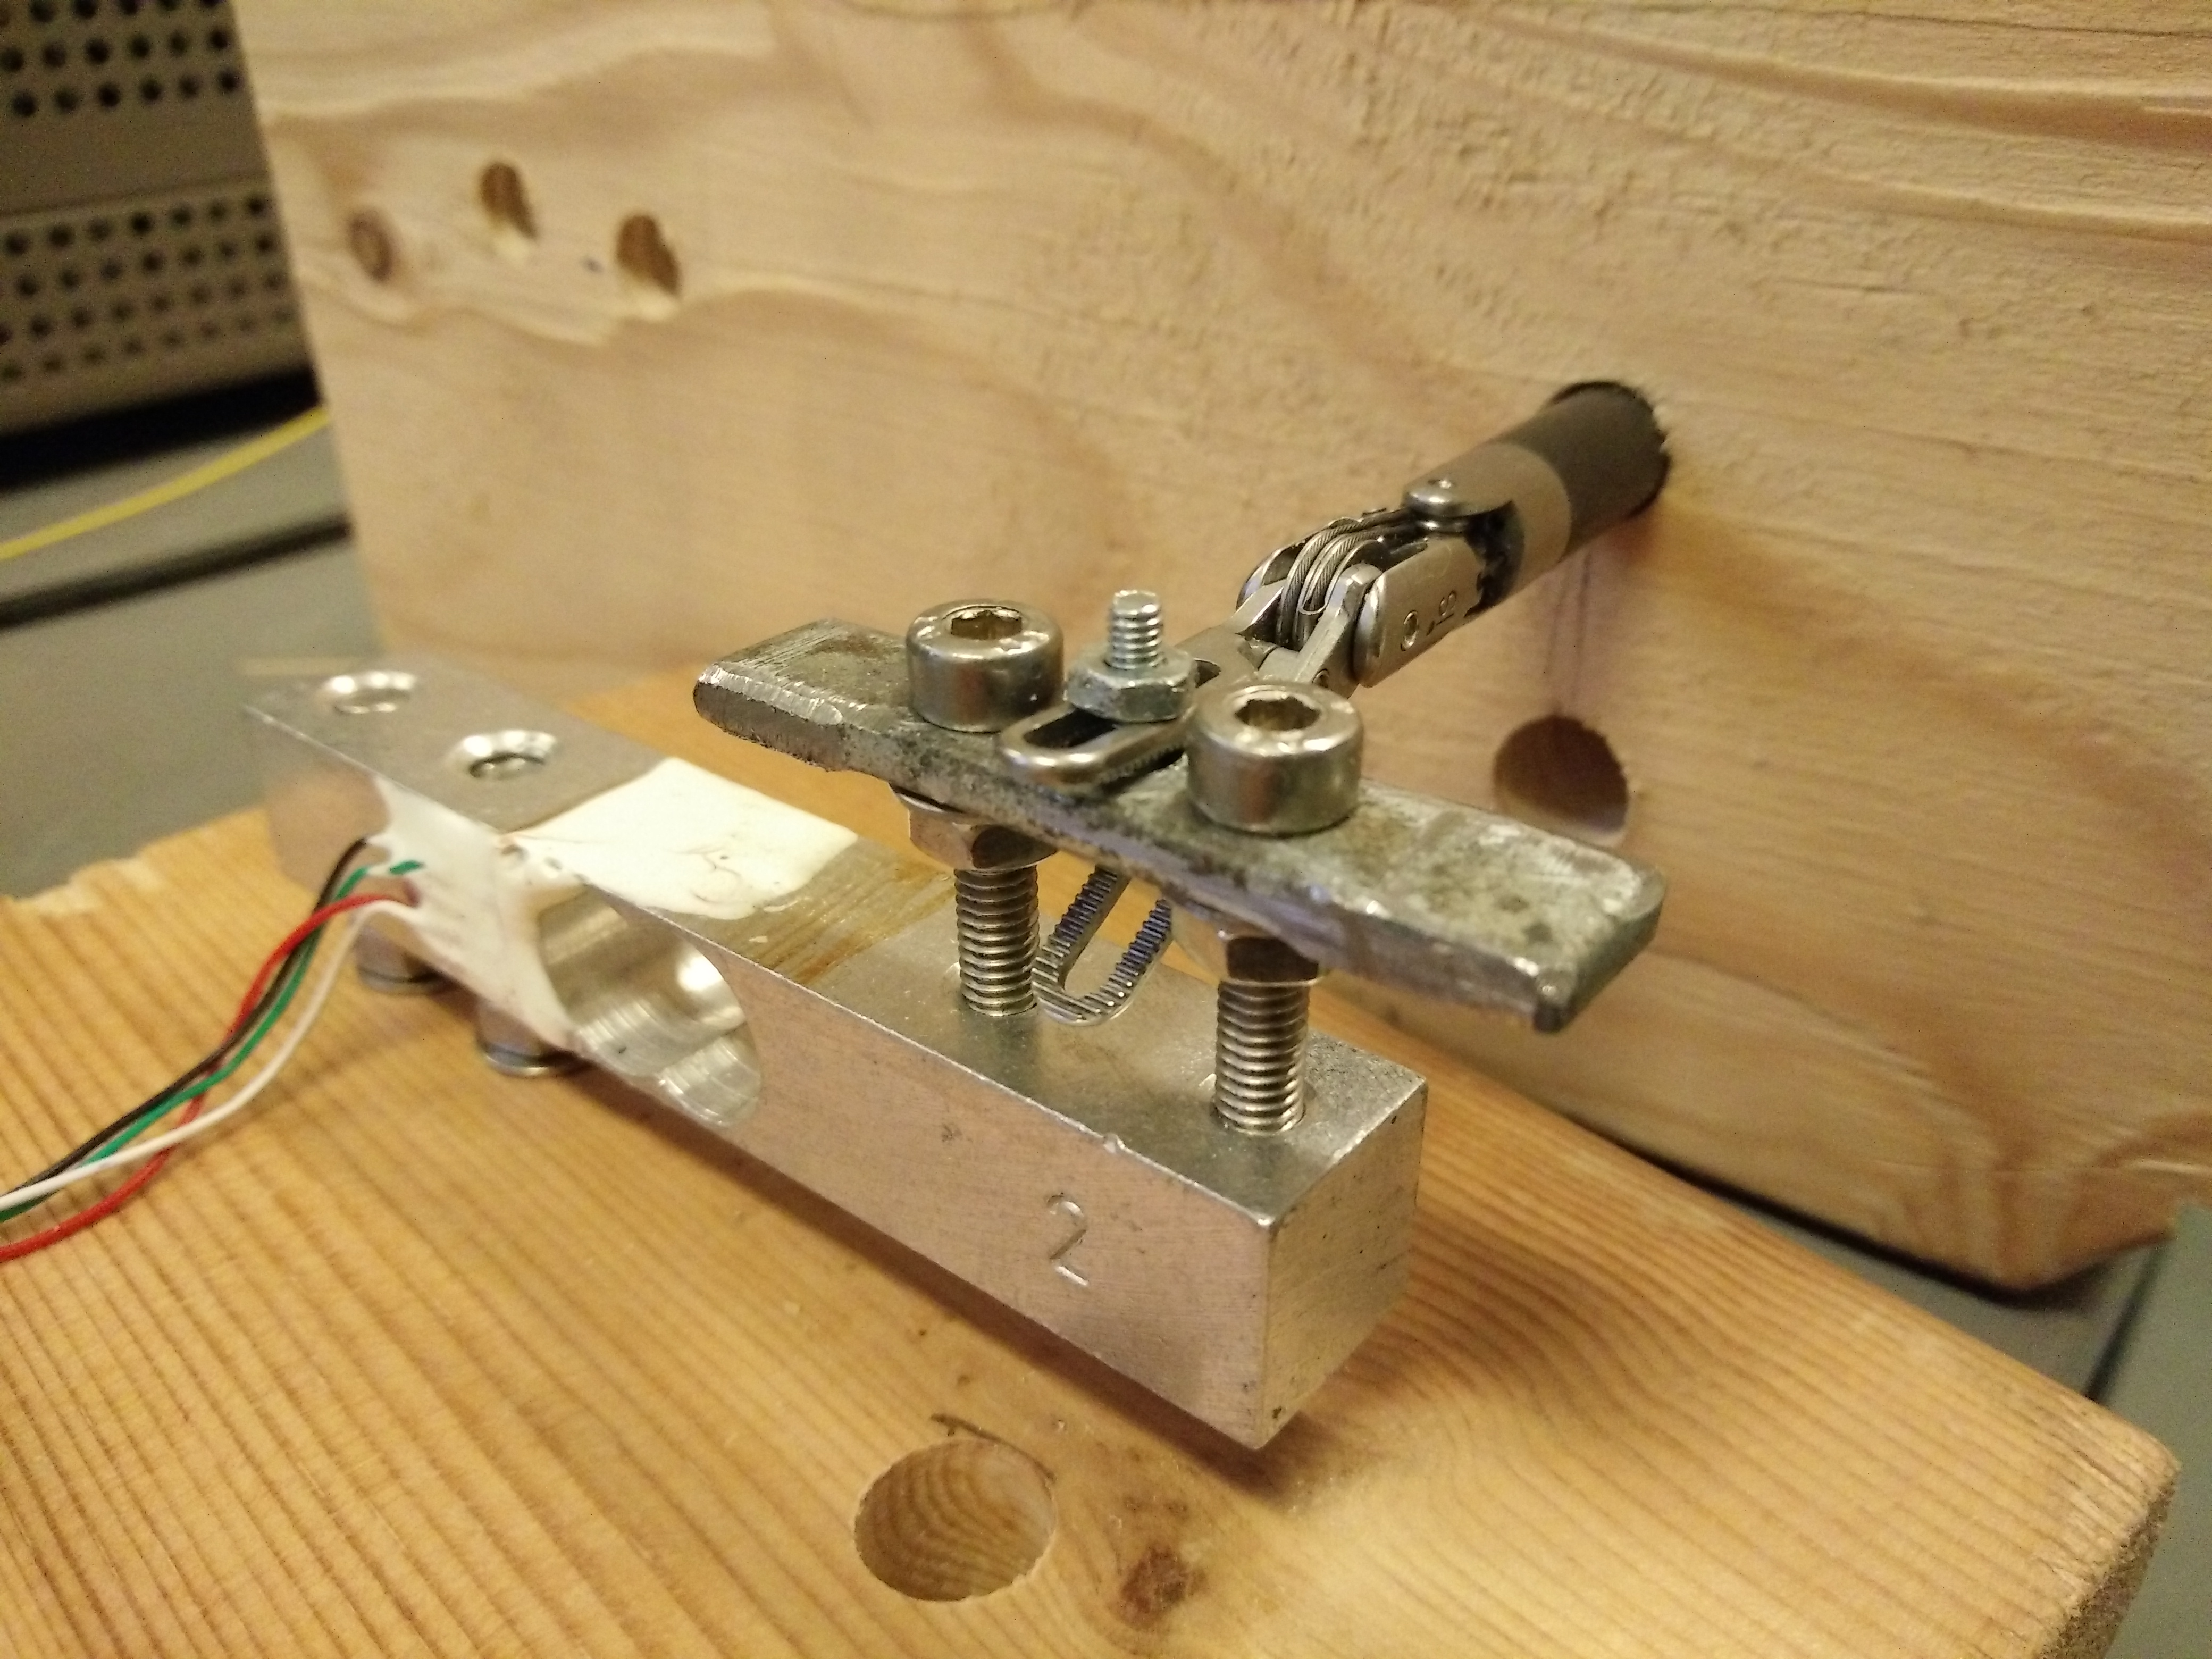
\includegraphics[width=\linewidth]{One_clamp.jpg} 
        \caption{Yaw} \label{fig:mes1}
    \end{subfigure}
    \begin{subfigure}[t]{0.32\textwidth}
        \centering
        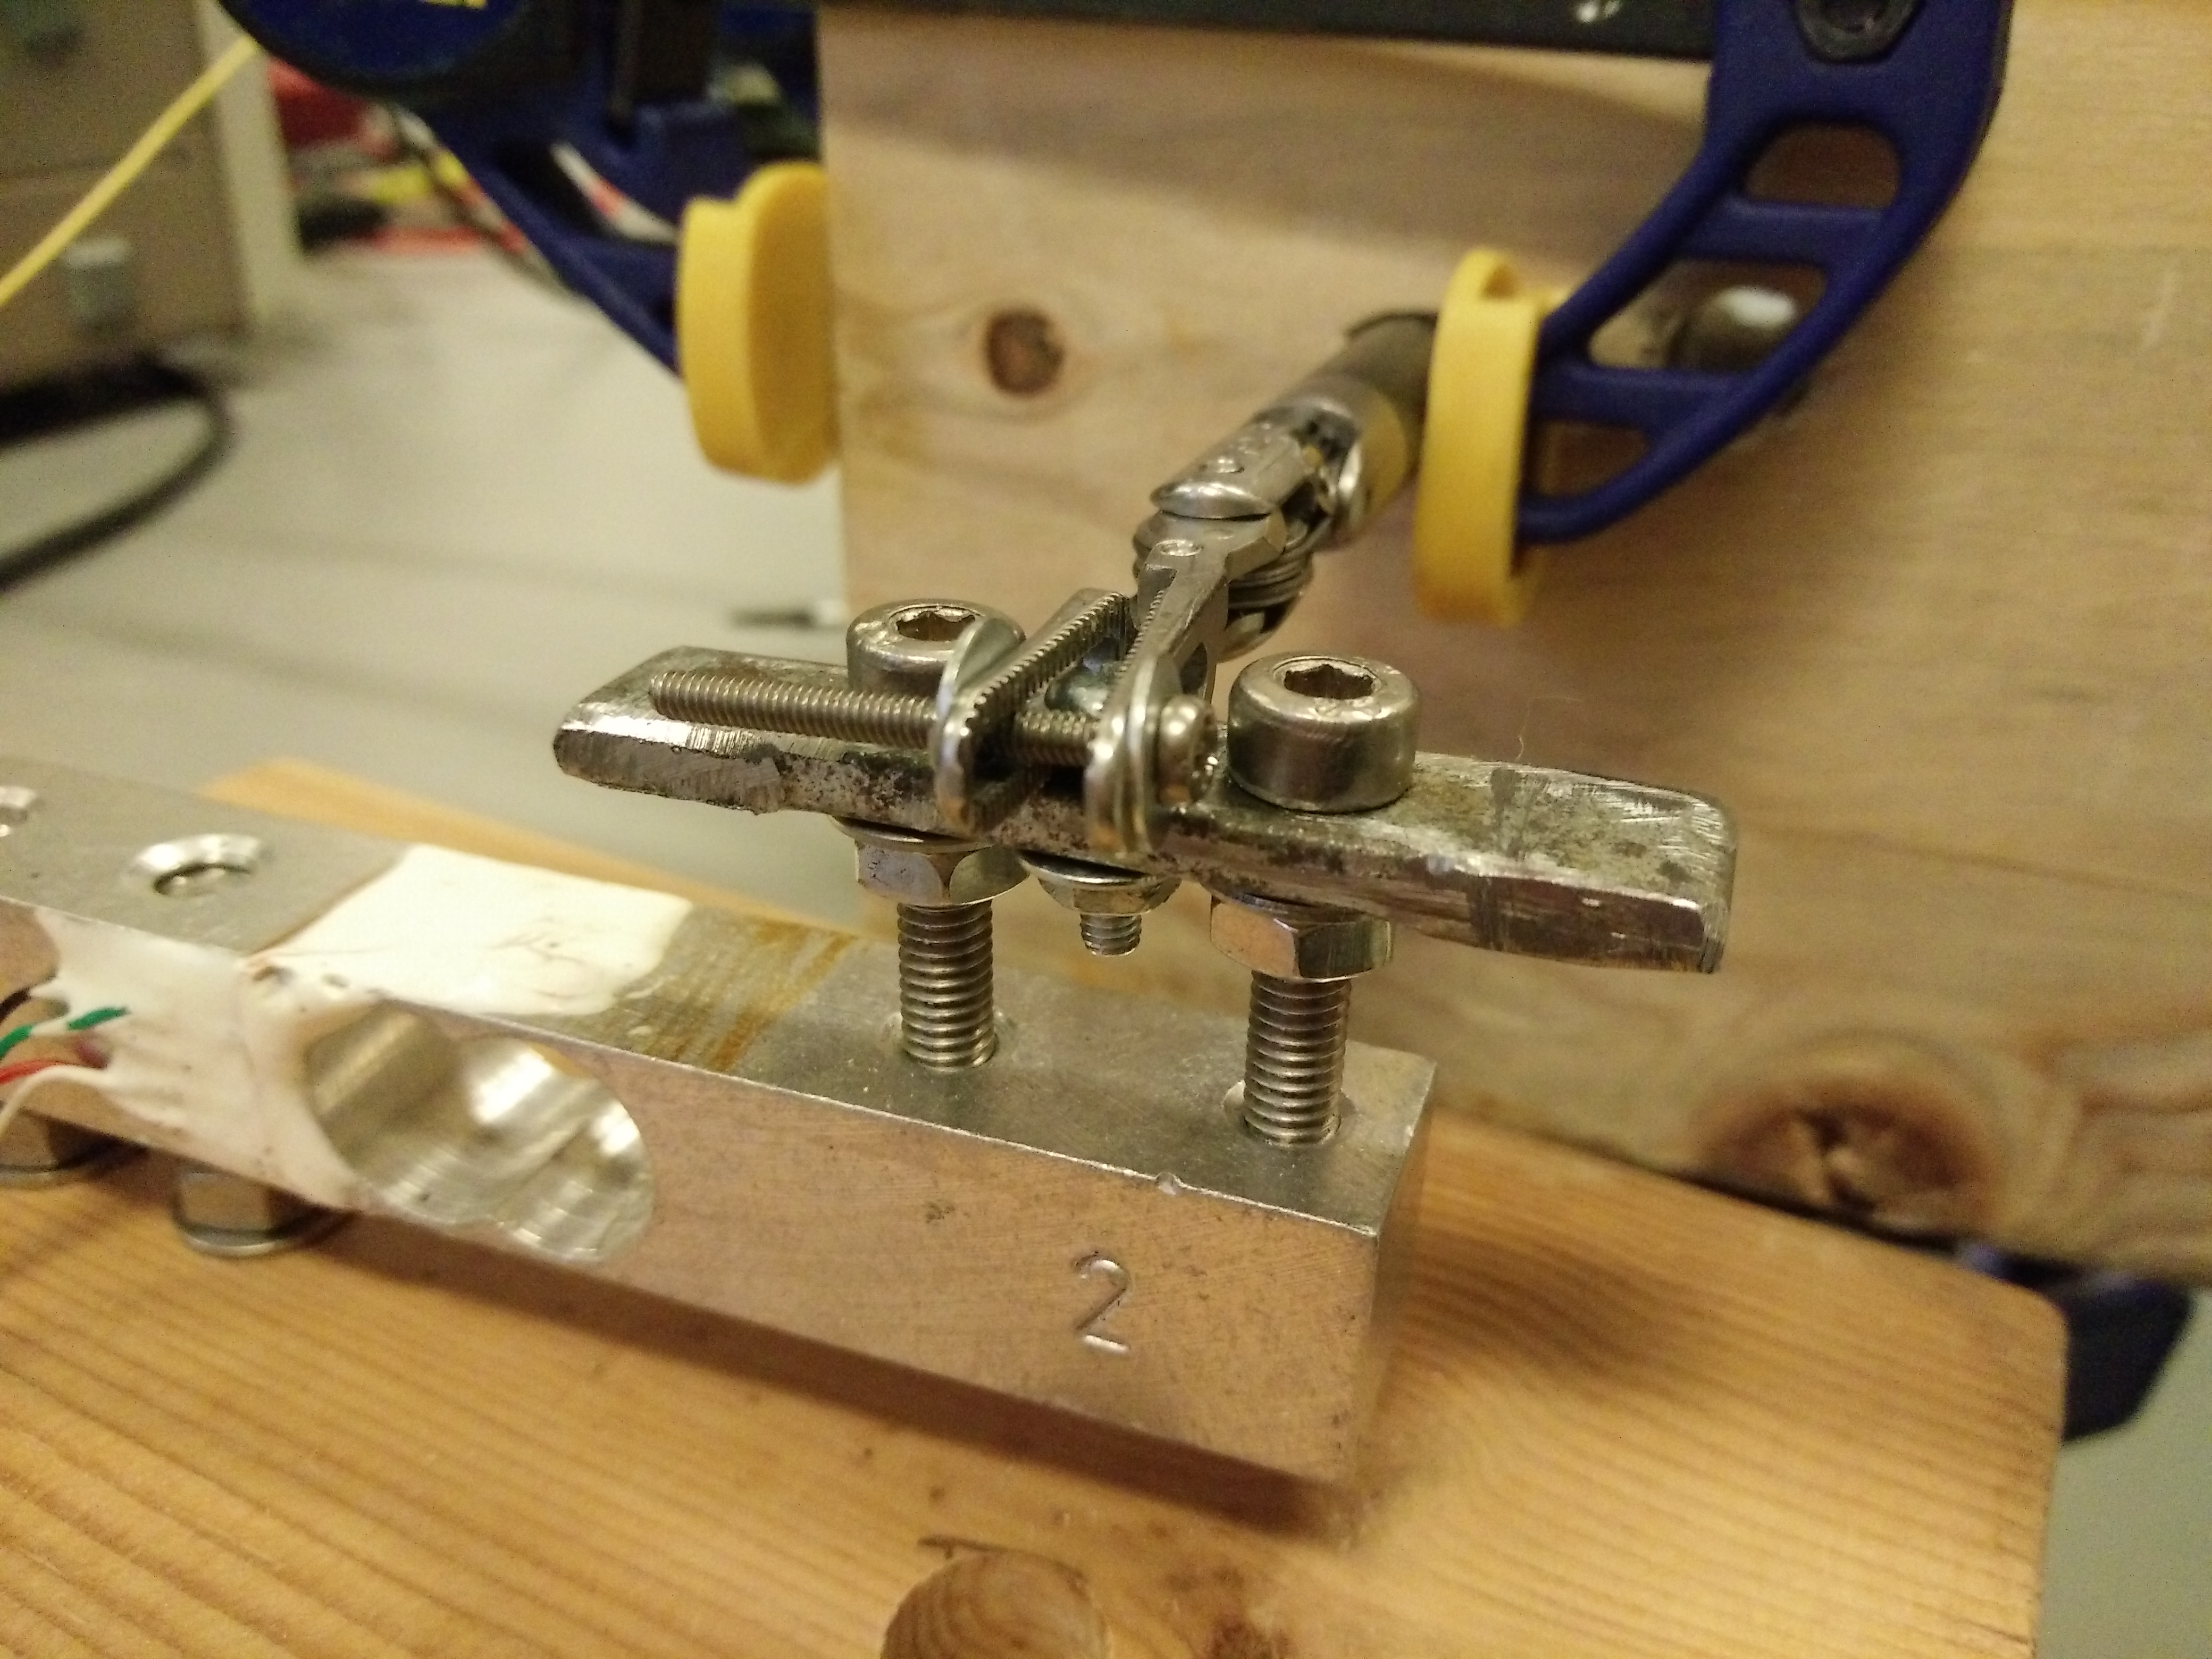
\includegraphics[width=\linewidth]{Pitch_clamp.jpg} 
        \caption{Pitch} \label{fig:mes2}
    \end{subfigure}
        \begin{subfigure}[t]{0.32\textwidth}
        \centering
        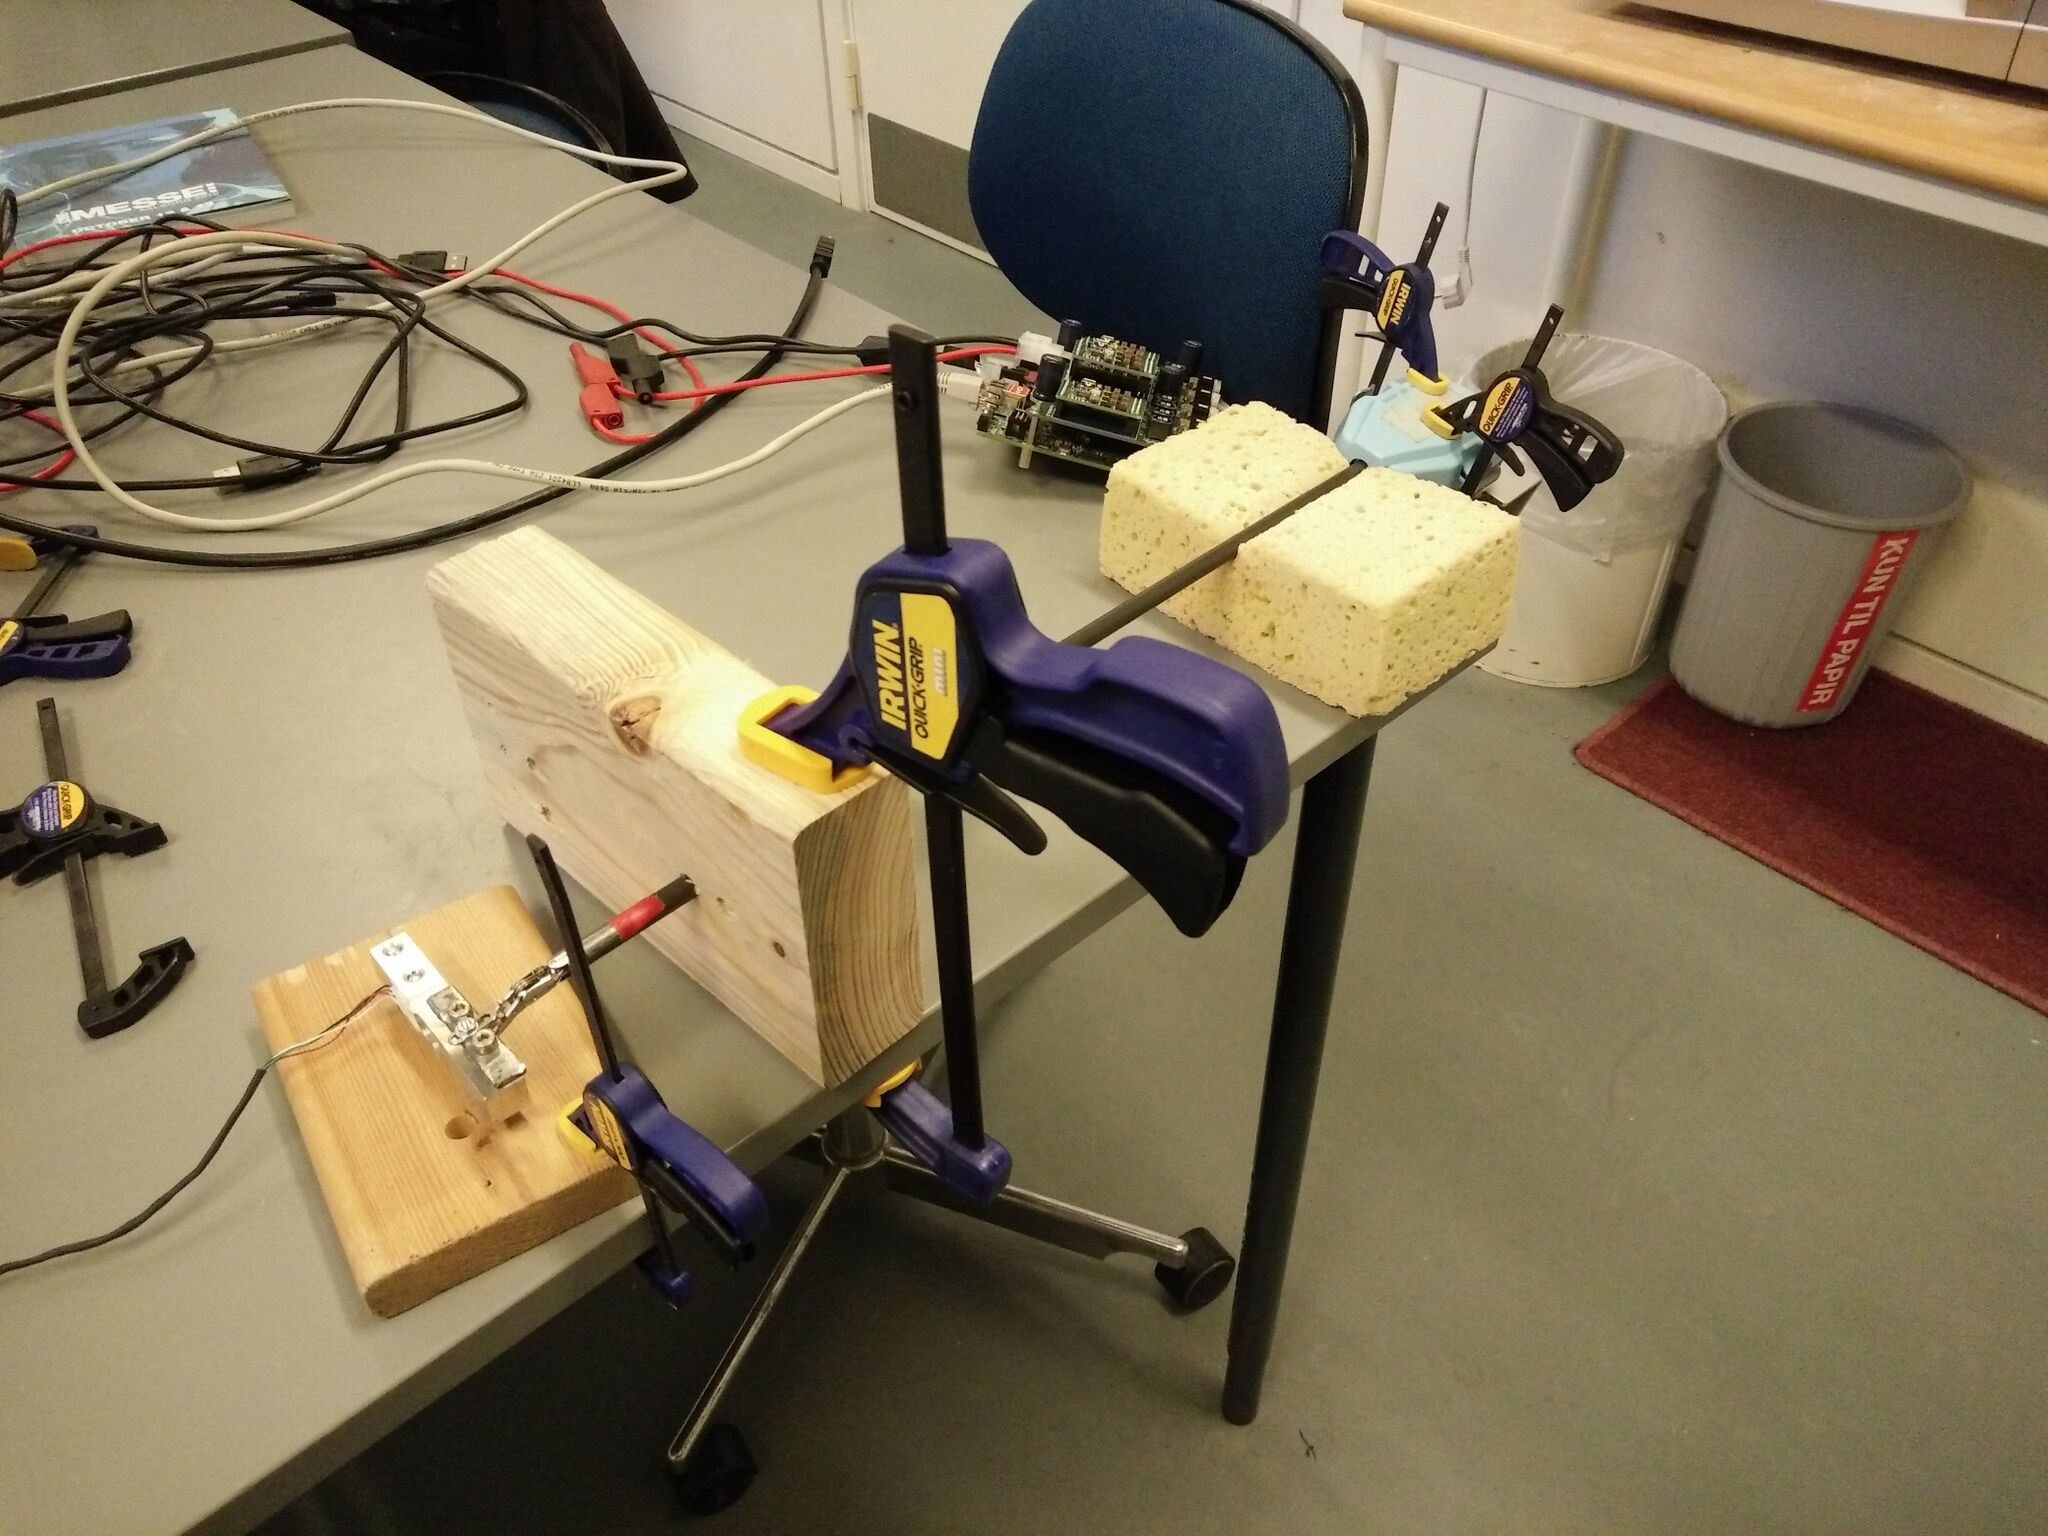
\includegraphics[width=\linewidth]{overall_force.jpg} 
        \caption{Full view} \label{fig:mes3}
    \end{subfigure}
\end{figure}
\end{frame}

% the license
\begin{frame}{Force estimation}{Model structure}

  \begin{itemize}
      \item Hammerstein-Wiener Model
	  \item Linear part is represented in state space
	  \item Nonlinearities on input and output can take different forms
	  \begin{itemize}
	  \item Deadzone, saturation ...
	  \item Neural networks
	  \end{itemize}
  \end{itemize}
%\end{column}%
%\hfill%
%\begin{column}{.65\textwidth}

\vspace{3em}
\begin{figure}[H]
\resizebox{0.9\textwidth}{!}{
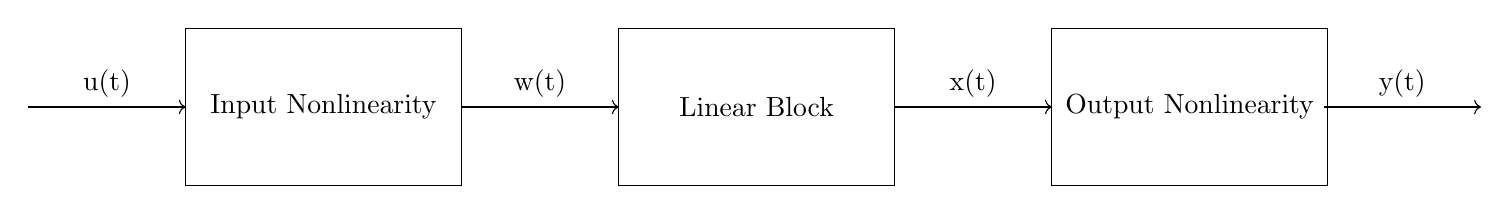
\begin{tikzpicture}
\draw  (-3.5,3) rectangle (0,1) node[pos=.5] {Linear Block};
\draw  (-9,3) rectangle (-5.5,1) node[pos=.5] {Input Nonlinearity};
\draw  (2,3) rectangle (5.5,1) node[pos=.5] {Output Nonlinearity};
\draw [->] (-5.5,2) -- (-3.5,2) node [pos=0.5,above] {w(t)};
\draw [->] (-11,2) -- (-9,2) node [pos=0.5,above] {u(t)};
\draw [->] (0,2) -- (2,2) node [pos=0.5,above] {x(t)};
\draw [->] (5.45,2) -- (7.45,2) node [pos=0.5,above] {y(t)};
\end{tikzpicture}
}
\caption{Hammerstein-Wiener model.}
\label{weiner}
\end{figure}


%\end{column}
%\end{columns}

\end{frame}



%%%%%%%%%%%%%%%%%%%%%%%%%%%%%%%%%%%%%%%%%%%%%%%%%%%%%%%%%%%%%%%%%%%%%%%%%%%%%%%%%%%

\begin{frame}{Force estimation}{Linear model}
\begin{itemize}
  \item Subspace identification
	\begin{itemize}
	\item Different algorithms: SSARX, CVA, MOESP
	\item Hankel singular value analysis used for picking order
	\end{itemize}
  \item Choice of inputs and data affects fit of model
  \item Inputs: effort, velocity 
  \item Outputs: force (, position error)
\end{itemize}
	
	\begin{figure}
	\centering
	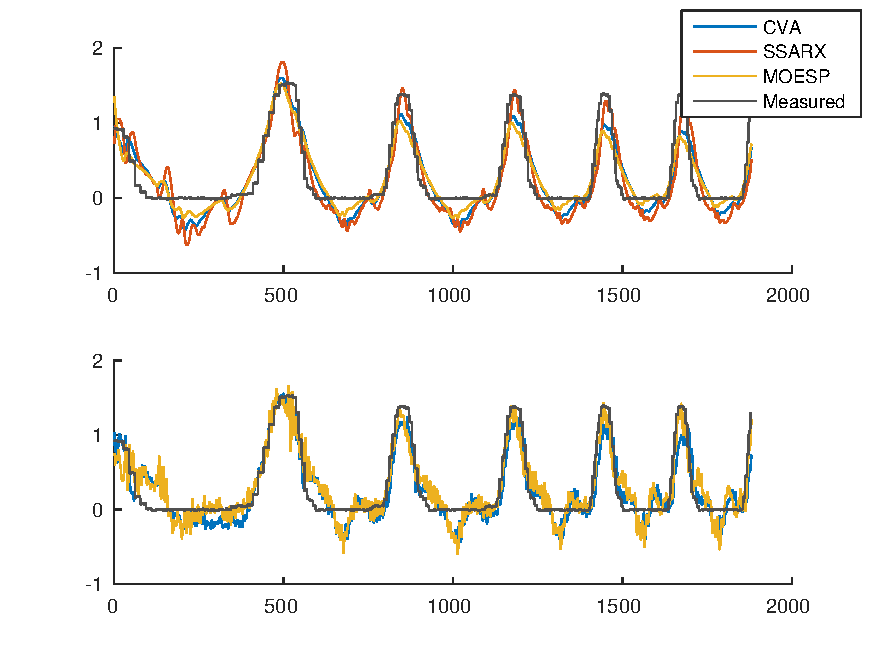
\includegraphics[width=\linewidth]{Billeder/sscomparison1-eps-converted-to.pdf}
	\end{figure}
\end{frame}

\begin{frame}{Force estimation}{Linear model}
\begin{itemize}
\item Roll model proportional to effort on actuator
\item 6th order linear models for both yaw and pitch
\begin{itemize}
\item Yaw model has good fit to data, sometimes underestimates amplitude
\item Pitch model fitting process suffered from disturbances in data and fit varies heavily
\end{itemize}
\end{itemize}
\begin{figure}
\centering
    \begin{subfigure}[t]{0.49\textwidth}
        \centering
        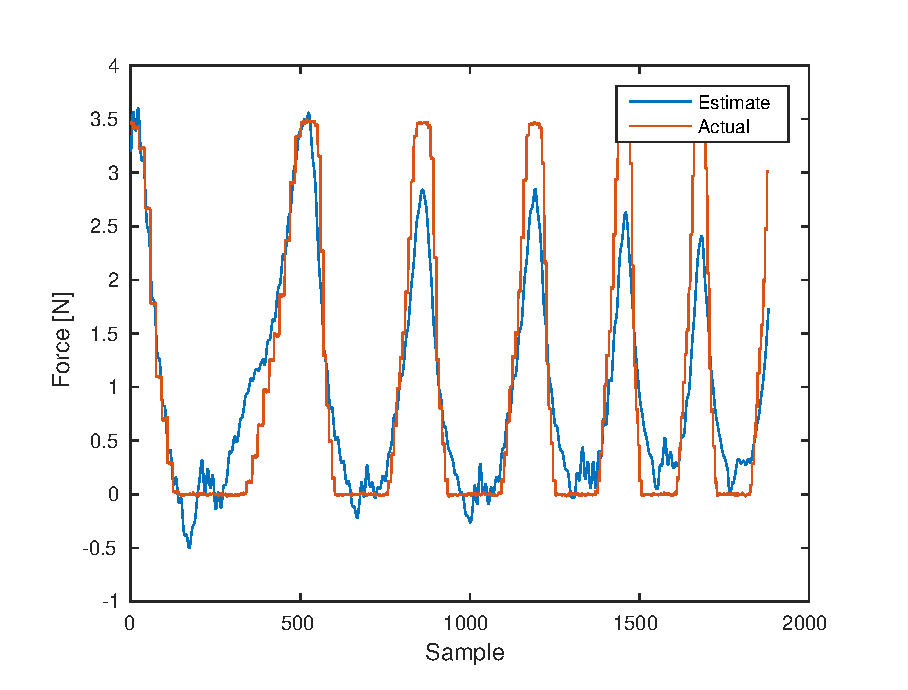
\includegraphics[width=\linewidth]{res_yaw} 
        \caption{Yaw} \label{fig:yawres}
    \end{subfigure}
        \begin{subfigure}[t]{0.49\textwidth}
        \centering
        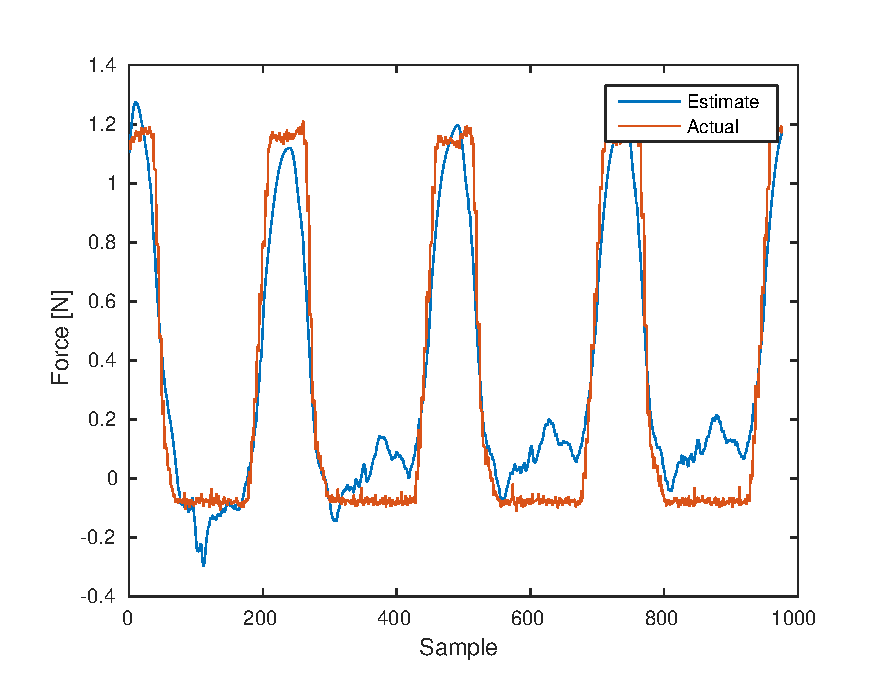
\includegraphics[width=\linewidth]{res_pitch} 
        \caption{Pitch} \label{fig:pitchres}
    \end{subfigure}
\end{figure}
\end{frame}

\begin{frame}{Force estimation}{Hammerstein Wiener Model}
\begin{itemize}
  \item Input and output nonlinearities
  \begin{itemize}
    \item Identified different types of nonlinearities (deadzone, saturation)
  \end{itemize}  
  \item Represent friction and elasticity effects
  \begin{itemize}
  	\item Also represents the environment the measurements were made in
  \end{itemize}
\end{itemize}

\begin{figure}
\centering
    \begin{subfigure}[t]{0.49\textwidth}
        \centering
        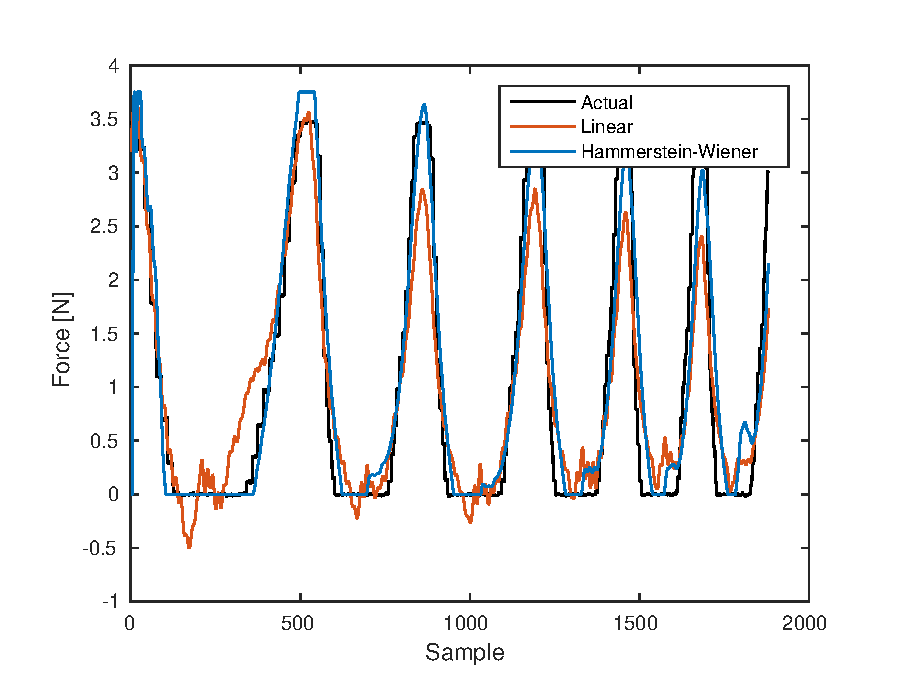
\includegraphics[width=\linewidth]{yawnl} 
        \caption{Yaw} \label{fig:yawresnl}
    \end{subfigure}
        \begin{subfigure}[t]{0.49\textwidth}
        \centering
        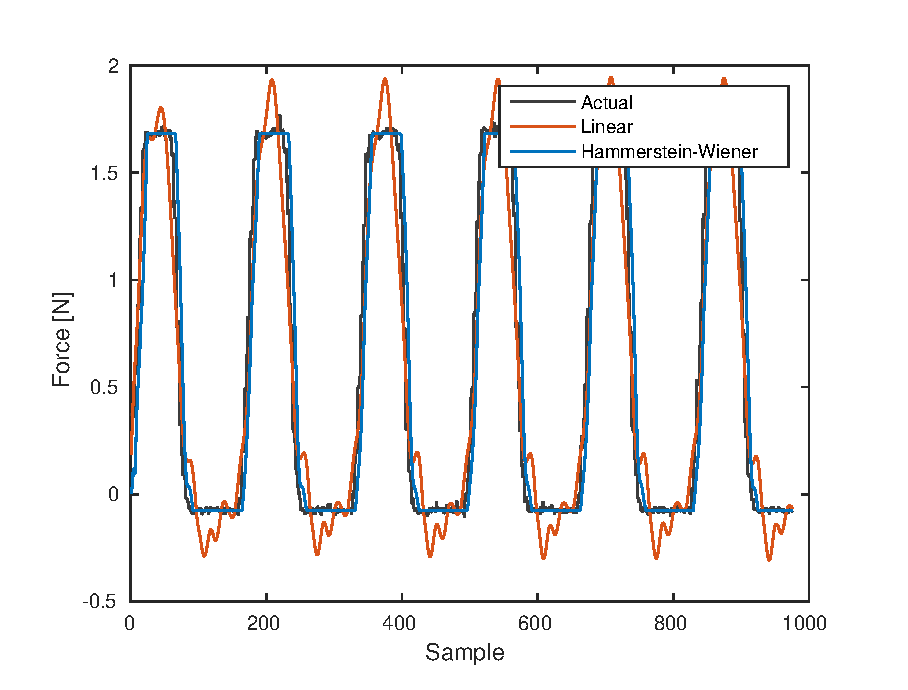
\includegraphics[width=\linewidth]{pitchnl} 
        \caption{Pitch} \label{fig:pitchresnl}
    \end{subfigure}
\end{figure}
\end{frame}

%chosen models


\begin{frame}{Force estimation}{Model correction}
\begin{itemize}
\item Idea: use a model that estimates position error along with force to correct force estimate
\begin{itemize}
\item Use Kalman filter to correct state and force estimates using position error measurements
\end{itemize}
\item Not able to achieve satisfying results with real data
\end{itemize}
\begin{figure}
\centering
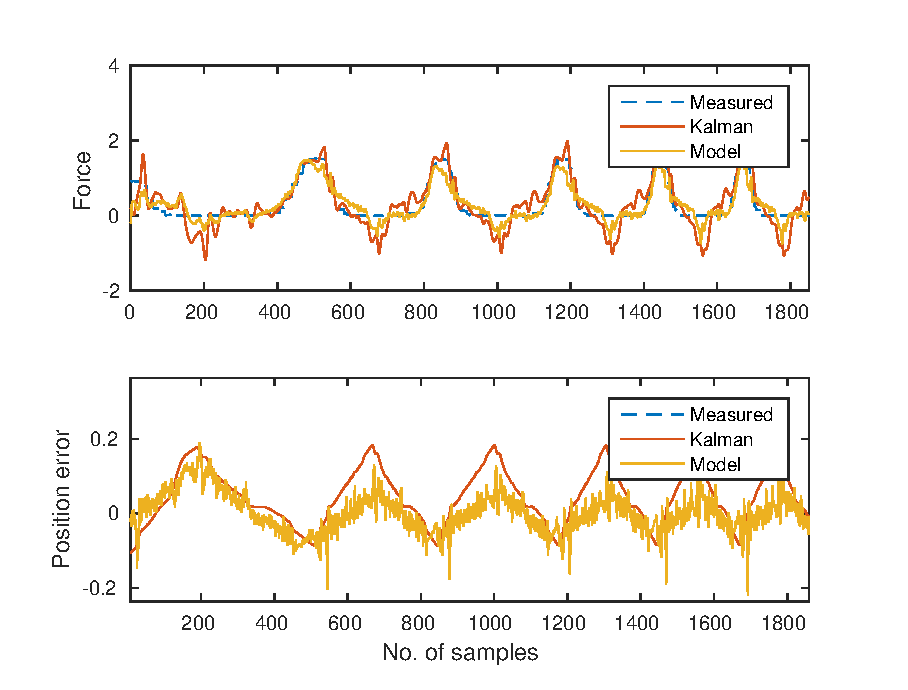
\includegraphics[width = 0.6\textwidth]{kl2}
\end{figure}
\end{frame}
%%%%%%%%%%



% in simulation part mention sliding mode control as an option to cure nonlinearities
%%%%%%%%%%%%%%%%%%%%%%%%%%%%%%%%
\section{Control Scheme}

\begin{frame}{Control Architecture}{}
  \begin{itemize}
    \item Two closed loops send reference signals mutually
    \item The architecture contains delays
    \item The force is estimated from the measured current and velocity
    \end{itemize}
    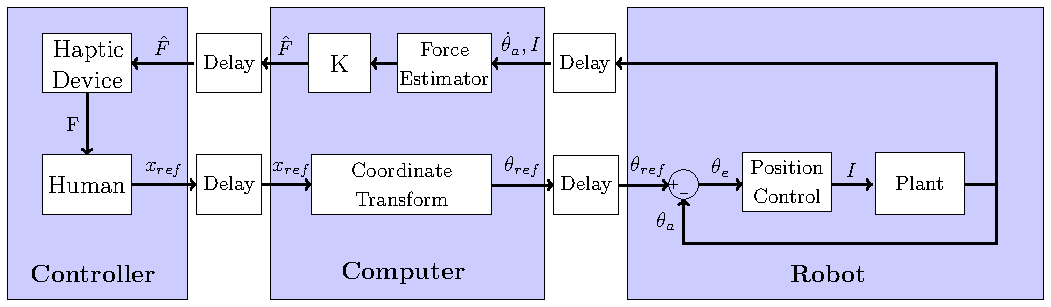
\includegraphics[width=\textwidth]{Billeder/Dan/control.pdf}
\end{frame}

%%%%%%%%%%%%%%%%%%%%%%%%%%%%%%%%
\section{Results}
%%%%%%%%%%%% MID WAY AGENDA %%%%%%%%%%%%%%
\begin{frame}{Results}{feedback response}<beamer>
\vspace*{1.5cm}
\begin{figure}
\centering
% This file was created by matlab2tikz.
%
%The latest updates can be retrieved from
%  http://www.mathworks.com/matlabcentral/fileexchange/22022-matlab2tikz-matlab2tikz
%where you can also make suggestions and rate matlab2tikz.
%
\definecolor{mycolor1}{rgb}{0.00000,0.44700,0.74100}%
\definecolor{mycolor2}{rgb}{0.85000,0.32500,0.09800}%
%
\begin{tikzpicture}

\begin{axis}[%
width=0.7\columnwidth,
height=0.45\columnwidth,
at={(2.512in,1.147in)},
scale only axis,
xmin=0,
xmax=14,
xlabel style={font=\color{white!15!black}},
xlabel={Time (s)},
ymin=-1,
ymax=2.6,
ylabel style={font=\color{white!15!black}},
ylabel={Amplitude},
axis background/.style={fill=white},
title style={font=\bfseries},
title={Force feedback response for the clamp},
xmajorgrids,
ymajorgrids,
legend style={legend cell align=left, align=left, draw=white!15!black, at={(0.66,0.25)}}
]

\addplot [color=mycolor1, draw=none, mark=*, mark size=1,mark options={solid, mycolor1}]
  table[row sep=crcr]{%
0	-0.069839\\
0.046	-0.0691929999999998\\
0.092	-0.0674169999999998\\
0.138	-0.0627580000000001\\
0.184	-0.0585599999999999\\
0.23	-0.053715\\
0.276	-0.052262\\
0.322	-0.0517779999999999\\
0.368	-0.0508089999999999\\
0.414	-0.050325\\
0.46	-0.0500019999999999\\
0.506	-0.0500019999999999\\
0.552	-0.0500019999999999\\
0.598	-0.0500019999999999\\
0.644	-0.050233\\
0.69	-0.0504629999999999\\
0.736	-0.0509360000000001\\
0.782	-0.0523979999999999\\
0.828	-0.0533170000000001\\
0.874	-0.0544640000000001\\
0.92	-0.0558380000000001\\
0.966	-0.059431\\
1.012	-0.0646089999999999\\
1.058	-0.069102\\
1.104	-0.070166\\
1.15	-0.0678619999999999\\
1.196	-0.0632820000000001\\
1.242	-0.0596559999999999\\
1.288	-0.054314\\
1.334	-0.045984\\
1.38	-0.0253700000000001\\
1.426	-0.00976399999999988\\
1.472	0.00805999999999996\\
1.518	0.0212249999999999\\
1.564	0.051482\\
1.61	0.0750869999999999\\
1.656	0.109672\\
1.702	0.138343\\
1.748	0.168177\\
1.794	0.199188\\
1.84	0.250473\\
1.886	0.306211\\
1.932	0.324103\\
1.978	0.347052\\
2.024	0.362787\\
2.07	0.383776\\
2.116	0.406007\\
2.162	0.449559\\
2.208	0.474824\\
2.254	0.508958\\
2.3	0.530804\\
2.346	0.554437\\
2.392	0.572537\\
2.438	0.591942\\
2.484	0.614258\\
2.53	0.625926\\
2.576	0.652916\\
2.622	0.665954\\
2.668	0.680707\\
2.714	0.6931054\\
2.76	0.7064931\\
2.806	0.7187228\\
2.852	0.7341136\\
2.898	0.7492224\\
2.944	0.7593239\\
2.99	0.7720971\\
3.036	0.7809118\\
3.082	0.7910974\\
3.128	0.8020223\\
3.174	0.81066\\
3.22	0.8186307\\
3.266	0.8319814\\
3.312	0.8492741\\
3.358	0.8558223\\
3.404	0.8646376\\
3.45	0.868742\\
3.496	0.8814436\\
3.542	0.8863328\\
3.588	0.8938385\\
3.634	0.9044656\\
3.68	0.9069801\\
3.726	0.9089659\\
3.772	0.9109976\\
3.818	0.9148639\\
3.864	0.9265554\\
3.91	0.9278963\\
3.956	0.9373217\\
4.002	0.940841\\
4.048	0.9445568\\
4.094	0.95726415\\
4.14	0.9604788\\
4.186	0.96597617\\
4.232	0.97119919\\
4.278	0.97641396\\
4.324	0.9801821\\
4.37	0.9838232\\
4.416	0.9907857\\
4.462	0.99572\\
4.508	0.9983443\\
4.554	1.0027004\\
4.6	1.0057562\\
4.646	1.0081051\\
4.692	1.0098843\\
4.738	1.0125273\\
4.784	1.0145615\\
4.83	1.015724\\
4.876	1.0164667\\
4.922	1.0164667\\
4.968	1.0164667\\
5.014	1.0164667\\
5.06	1.0164667\\
5.106	1.0164667\\
5.152	1.0164667\\
5.198	1.017048\\
5.244	1.0196638\\
5.29	1.0246052\\
5.336	1.0286748\\
5.382	1.0344887\\
5.428	1.0368141\\
5.474	1.0379768\\
5.52	1.0385582\\
5.566	1.0385582\\
5.612	1.0385582\\
5.658	1.0391396\\
5.704	1.0420462\\
5.75	1.045534\\
5.796	1.0490214\\
5.842	1.0522178\\
5.888	1.0536705\\
5.934	1.0571568\\
5.98	1.059633\\
6.026	1.062445\\
6.072	1.0644935\\
6.118	1.0679936\\
6.164	1.0718006\\
6.21	1.0739226\\
6.256	1.0760766\\
6.302	1.0773746\\
6.348	1.0781606\\
6.394	1.0786866\\
6.44	1.0796386\\
6.486	1.0806226\\
6.532	1.0811326\\
6.578	1.0815816\\
6.624	1.0821676\\
6.67	1.0826356\\
6.716	1.0836156\\
6.762	1.0849286\\
6.808	1.0862066\\
6.854	1.0874876\\
6.9	1.0889816\\
6.946	1.0904386\\
6.992	1.0921886\\
7.038	1.0943516\\
7.084	1.0958206\\
7.13	1.0971756\\
7.176	1.0983656\\
7.222	1.0995076\\
7.268	1.1005966\\
7.314	1.1015086\\
7.36	1.1031166\\
7.406	1.1045566\\
7.452	1.1057716\\
7.498	1.1059546\\
7.544	1.1072416\\
7.59	1.1076566\\
7.636	1.1080086\\
7.682	1.1083606\\
7.728	1.1083606\\
7.774	1.1082496\\
7.82	1.1082496\\
7.866	1.1078506\\
7.912	1.1055066\\
7.958	1.1023436\\
8.004	1.0977176\\
8.05	1.0940366\\
8.096	1.0909596\\
8.142	1.0861036\\
8.188	1.0816106\\
8.234	1.0766646\\
8.28	1.0723386\\
8.326	1.0637863\\
8.372	1.0543818\\
8.418	1.0428257\\
8.464	1.029448\\
8.51	1.0175659\\
8.556	1.0002029\\
8.602	0.9837055\\
8.648	0.97187785\\
8.694	0.96156563\\
8.74	0.9554396\\
8.786	0.942303\\
8.832	0.9318928\\
8.878	0.9191614\\
8.924	0.9095359\\
8.97	0.9029574\\
9.016	0.8912888\\
9.062	0.879097\\
9.108	0.8563865\\
9.154	0.8307516\\
9.2	0.8113894\\
9.246	0.7837317\\
9.292	0.7592755\\
9.338	0.725409\\
9.384	0.691096\\
9.43	0.659743\\
9.476	0.635184\\
9.522	0.599631\\
9.568	0.572746\\
9.614	0.537474\\
9.66	0.488529\\
9.706	0.470013\\
9.752	0.449131\\
9.798	0.434072\\
9.844	0.412879\\
9.89	0.394881\\
9.936	0.372667\\
9.982	0.354272\\
10.028	0.320757\\
10.074	0.287993\\
10.12	0.232964\\
10.166	0.197741\\
10.212	0.18275\\
10.258	0.156795\\
10.304	0.138484\\
10.35	0.114872\\
10.396	0.097008\\
10.442	0.071595\\
10.488	0.05155\\
10.534	0.034095\\
10.58	0.0179400000000001\\
10.626	0.002305\\
10.672	-0.00167099999999998\\
10.718	-0.00769699999999984\\
10.764	-0.030978\\
10.81	-0.0429710000000001\\
10.856	-0.053148\\
10.902	-0.0618189999999998\\
10.948	-0.0720810000000001\\
10.994	-0.0724389999999999\\
11.04	-0.0717700000000001\\
11.086	-0.0703040000000001\\
11.132	-0.068948\\
11.178	-0.0678830000000001\\
11.224	-0.067339\\
11.27	-0.067339\\
11.316	-0.067339\\
11.362	-0.0671580000000001\\
11.408	-0.0669960000000001\\
11.454	-0.065239\\
11.5	-0.063358\\
11.546	-0.0595410000000001\\
11.592	-0.054964\\
11.638	-0.052603\\
11.684	-0.051604\\
11.73	-0.0518610000000002\\
11.776	-0.053331\\
11.822	-0.0551919999999999\\
11.868	-0.0570810000000002\\
11.914	-0.059763\\
11.96	-0.0673490000000001\\
12.006	-0.075137\\
12.052	-0.0787260000000001\\
12.098	-0.084632\\
12.144	-0.090457\\
12.19	-0.099099\\
12.236	-0.115104\\
12.282	-0.138322\\
12.328	-0.147654\\
12.374	-0.150269\\
12.42	-0.156016\\
12.466	-0.1626\\
12.512	-0.166108\\
12.558	-0.169979\\
12.604	-0.172681\\
12.65	-0.176454\\
12.696	-0.177723\\
12.742	-0.178345\\
12.788	-0.179376\\
12.834	-0.178237\\
12.88	-0.176378\\
12.926	-0.175254\\
12.972	-0.174123\\
13.018	-0.172999\\
13.064	-0.171682\\
13.11	-0.167706\\
13.156	-0.164679\\
13.202	-0.157745\\
13.248	-0.1501\\
13.294	-0.127712\\
13.34	-0.106903\\
13.386	-0.0901689999999999\\
13.432	-0.0812360000000001\\
13.478	-0.0620539999999998\\
13.524	-0.0516510000000001\\
13.57	-0.035822\\
13.616	-0.029779\\
13.662	-0.0236429999999999\\
13.708	-0.0221900000000002\\
13.754	-0.0202520000000002\\
13.8	-0.0181120000000001\\
13.846	-0.018038\\
13.892	-0.018243\\
13.938	-0.0184470000000001\\
13.984	-0.019682\\
14.03	-0.0207010000000001\\
14.076	-0.0221230000000001\\
14.122	-0.023096\\
14.168	-0.023096\\
14.214	-0.023096\\
14.26	-0.0234529999999999\\
14.306	-0.024132\\
14.352	-0.0254239999999999\\
14.398	-0.0299449999999999\\
14.444	-0.033693\\
14.49	-0.0363100000000001\\
14.536	-0.0374399999999999\\
14.582	-0.0393779999999999\\
14.628	-0.039701\\
14.674	-0.0398689999999999\\
14.72	-0.0398770000000002\\
14.766	-0.039682\\
14.812	-0.039682\\
14.858	-0.039682\\
14.904	-0.039682\\
14.95	-0.039682\\
14.996	-0.0391299999999999\\
15.042	-0.0387390000000001\\
15.088	-0.0385439999999999\\
15.134	-0.038152\\
15.18	-0.0377609999999999\\
15.226	-0.0377609999999999\\
15.272	-0.0377609999999999\\
15.318	-0.0377609999999999\\
15.364	-0.0377609999999999\\
15.41	-0.0377609999999999\\
15.456	-0.0375649999999998\\
15.502	-0.0375649999999998\\
15.548	-0.036365\\
15.594	-0.0331220000000001\\
15.64	-0.030756\\
15.686	-0.0297510000000001\\
15.732	-0.02959\\
15.778	-0.028459\\
};
\addlegendentry{Position Error}

\addplot [color=mycolor2, thick]
  table[row sep=crcr]{%
0	-0.457965\\
0.046	-0.482939\\
0.092	-0.512125\\
0.138	-0.528618\\
0.184	-0.539522\\
0.23	-0.537151\\
0.276	-0.524402\\
0.322	-0.507127\\
0.368	-0.470289\\
0.414	-0.428809\\
0.46	-0.387254\\
0.506	-0.339716\\
0.552	-0.303282\\
0.598	-0.26139\\
0.644	-0.235044\\
0.69	-0.212801\\
0.736	-0.186553\\
0.782	-0.161903\\
0.828	-0.14172\\
0.874	-0.120005\\
0.92	-0.094566\\
0.966	-0.0684803\\
1.012	-0.0608241\\
1.058	-0.0433587\\
1.104	-0.0174891\\
1.15	-0.00521286\\
1.196	0.000178016\\
1.242	-0.00297375\\
1.288	-0.0138918\\
1.334	-0.026421\\
1.38	-0.0261145\\
1.426	-0.0405375\\
1.472	-0.0576523\\
1.518	-0.0799315\\
1.564	-0.0976721\\
1.61	-0.0951568\\
1.656	-0.0724242\\
1.702	-0.0633538\\
1.748	-0.0541451\\
1.794	-0.021039\\
1.84	0.000387498\\
1.886	0.00063466\\
1.932	0.000510842\\
1.978	1.40871e-05\\
2.024	0.0176141\\
2.07	0.0641683\\
2.116	0.109299\\
2.162	0.152024\\
2.208	0.179542\\
2.254	0.185892\\
2.3	0.191742\\
2.346	0.185386\\
2.392	0.189675\\
2.438	0.193986\\
2.484	0.230854\\
2.53	0.257935\\
2.576	0.303503\\
2.622	0.357063\\
2.668	0.390772\\
2.714	0.405952\\
2.76	0.443154\\
2.806	0.452801\\
2.852	0.481958\\
2.898	0.503039\\
2.944	0.527297\\
2.99	0.56528\\
3.036	0.591189\\
3.082	0.645425\\
3.128	0.670379\\
3.174	0.699748\\
3.22	0.735109\\
3.266	0.774628\\
3.312	0.805072\\
3.358	0.83938\\
3.404	0.882872\\
3.45	0.942162\\
3.496	0.967106\\
3.542	1.02907\\
3.588	1.07135\\
3.634	1.11914\\
3.68	1.16782\\
3.726	1.22586\\
3.772	1.26648\\
3.818	1.32544\\
3.864	1.36167\\
3.91	1.41453\\
3.956	1.45284\\
4.002	1.50118\\
4.048	1.55186\\
4.094	1.58921\\
4.14	1.63147\\
4.186	1.67488\\
4.232	1.71576\\
4.278	1.75288\\
4.324	1.79633\\
4.37	1.84079\\
4.416	1.88369\\
4.462	1.92324\\
4.508	1.96243\\
4.554	1.99936\\
4.6	2.02567\\
4.646	2.05945\\
4.692	2.08038\\
4.738	2.10928\\
4.784	2.13069\\
4.83	2.15696\\
4.876	2.17937\\
4.922	2.19947\\
4.968	2.21219\\
5.014	2.24018\\
5.06	2.26189\\
5.106	2.27821\\
5.152	2.29389\\
5.198	2.3042\\
5.244	2.31804\\
5.29	2.32692\\
5.336	2.33094\\
5.382	2.34414\\
5.428	2.35817\\
5.474	2.36845\\
5.52	2.38155\\
5.566	2.39363\\
5.612	2.40496\\
5.658	2.40824\\
5.704	2.41806\\
5.75	2.42631\\
5.796	2.4351\\
5.842	2.43808\\
5.888	2.45076\\
5.934	2.45048\\
5.98	2.45716\\
6.026	2.4668\\
6.072	2.46822\\
6.118	2.46973\\
6.164	2.47081\\
6.21	2.48353\\
6.256	2.48696\\
6.302	2.49787\\
6.348	2.5\\
6.394	2.5\\
6.44	2.5\\
6.486	2.5\\
6.532	2.49992\\
6.578	2.5\\
6.624	2.5\\
6.67	2.5\\
6.716	2.5\\
6.762	2.5\\
6.808	2.5\\
6.854	2.5\\
6.9	2.5\\
6.946	2.5\\
6.992	2.5\\
7.038	2.5\\
7.084	2.5\\
7.13	2.5\\
7.176	2.5\\
7.222	2.5\\
7.268	2.5\\
7.314	2.5\\
7.36	2.5\\
7.406	2.5\\
7.452	2.5\\
7.498	2.5\\
7.544	2.5\\
7.59	2.5\\
7.636	2.5\\
7.682	2.5\\
7.728	2.5\\
7.774	2.5\\
7.82	2.5\\
7.866	2.5\\
7.912	2.5\\
7.958	2.5\\
8.004	2.5\\
8.05	2.5\\
8.096	2.5\\
8.142	2.5\\
8.188	2.5\\
8.234	2.5\\
8.28	2.5\\
8.326	2.5\\
8.372	2.5\\
8.418	2.5\\
8.464	2.5\\
8.51	2.5\\
8.556	2.5\\
8.602	2.5\\
8.648	2.5\\
8.694	2.5\\
8.74	2.5\\
8.786	2.5\\
8.832	2.5\\
8.878	2.5\\
8.924	2.5\\
8.97	2.5\\
9.016	2.5\\
9.062	2.5\\
9.108	2.5\\
9.154	2.5\\
9.2	2.5\\
9.246	2.5\\
9.292	2.5\\
9.338	2.5\\
9.384	2.5\\
9.43	2.45972\\
9.476	2.31758\\
9.522	2.14825\\
9.568	1.99722\\
9.614	1.85379\\
9.66	1.72876\\
9.706	1.60717\\
9.752	1.51777\\
9.798	1.42349\\
9.844	1.34486\\
9.89	1.24209\\
9.936	1.13853\\
9.982	1.0087\\
10.028	0.888403\\
10.074	0.786921\\
10.12	0.712798\\
10.166	0.633521\\
10.212	0.58201\\
10.258	0.510575\\
10.304	0.442393\\
10.35	0.369444\\
10.396	0.293081\\
10.442	0.220909\\
10.488	0.152474\\
10.534	0.078849\\
10.58	0.0342911\\
10.626	0.000124028\\
10.672	0.000301921\\
10.718	0.000252726\\
10.764	0.000330059\\
10.81	0.000273753\\
10.856	-0.0174561\\
10.902	-0.0569983\\
10.948	-0.101156\\
10.994	-0.137496\\
11.04	-0.16853\\
11.086	-0.20015\\
11.132	-0.233028\\
11.178	-0.269616\\
11.224	-0.309738\\
11.27	-0.335806\\
11.316	-0.366884\\
11.362	-0.387696\\
11.408	-0.416516\\
11.454	-0.432208\\
11.5	-0.445834\\
11.546	-0.45736\\
11.592	-0.45423\\
11.638	-0.440815\\
11.684	-0.428176\\
11.73	-0.413655\\
11.776	-0.377847\\
11.822	-0.346186\\
11.868	-0.30626\\
11.914	-0.261468\\
11.96	-0.224553\\
12.006	-0.188972\\
12.052	-0.146403\\
12.098	-0.116957\\
12.144	-0.0867584\\
12.19	-0.0573152\\
12.236	-0.0552171\\
12.282	-0.0574377\\
12.328	-0.0575676\\
12.374	-0.0349744\\
12.42	-0.046042\\
12.466	-0.0523814\\
12.512	-0.0740595\\
12.558	-0.101582\\
12.604	-0.151553\\
12.65	-0.197503\\
12.696	-0.243833\\
12.742	-0.288091\\
12.788	-0.321104\\
12.834	-0.352334\\
12.88	-0.379869\\
12.926	-0.410188\\
12.972	-0.449443\\
13.018	-0.483054\\
13.064	-0.523156\\
13.11	-0.558781\\
13.156	-0.606164\\
13.202	-0.644778\\
13.248	-0.689715\\
13.294	-0.72931\\
13.34	-0.729152\\
13.386	-0.749485\\
13.432	-0.779093\\
13.478	-0.786947\\
13.524	-0.753038\\
13.57	-0.730523\\
13.616	-0.695568\\
13.662	-0.65353\\
13.708	-0.595233\\
13.754	-0.50868\\
13.8	-0.441981\\
13.846	-0.355192\\
13.892	-0.275813\\
13.938	-0.196536\\
13.984	-0.125382\\
14.03	-0.0564939\\
14.076	0.000372308\\
14.122	0.000553329\\
14.168	0.000643569\\
14.214	0.000462548\\
14.26	0.00539057\\
14.306	0.0388688\\
14.352	0.0787901\\
14.398	0.106753\\
14.444	0.130374\\
14.49	0.152278\\
14.536	0.170294\\
14.582	0.159808\\
14.628	0.155049\\
14.674	0.143513\\
14.72	0.12149\\
14.766	0.0911616\\
14.812	0.0673271\\
14.858	0.0494943\\
14.904	0.0241393\\
14.95	0.00996927\\
14.996	0.000383604\\
15.042	1.06228e-05\\
15.088	0.000199578\\
15.134	0.00057731\\
15.18	0.000486604\\
15.226	0.000296169\\
15.272	0.000202064\\
15.318	0.000297389\\
15.364	0.000202064\\
15.41	0.000297389\\
15.456	0.000682615\\
15.502	0.000490612\\
15.548	0.000398122\\
15.594	0.00049462\\
15.64	0.000399735\\
15.686	0.000596488\\
15.732	0.000108347\\
15.778	0.000401348\\
};
\addlegendentry{Force feedback [N]}

\addplot [color=green, dashed, very thick]
  table[row sep=crcr]{%
0	-0.0462933\\
0.046	-0.0146618\\
0.092	0.00131416\\
0.138	0.0156918\\
0.184	0.0268745\\
0.23	0.0278339\\
0.276	0.0204849\\
0.322	0.027195\\
0.368	0.0300694\\
0.414	0.0303898\\
0.46	0.026556\\
0.506	0.0262356\\
0.552	0.0275135\\
0.598	0.0217628\\
0.644	0.0211239\\
0.69	0.026556\\
0.736	0.0195255\\
0.782	0.0188866\\
0.828	0.0115376\\
0.874	-0.00220108\\
0.92	-0.00891113\\
0.966	-0.0418205\\
1.012	-0.0236073\\
1.058	-0.0344715\\
1.104	-0.0450153\\
1.15	-0.0504456\\
1.196	-0.0485287\\
1.242	-0.0261631\\
1.288	0.0057869\\
1.334	0.0434895\\
1.38	0.0380573\\
1.426	0.081192\\
1.472	0.129118\\
1.518	0.168417\\
1.564	0.209953\\
1.61	0.222414\\
1.656	0.213787\\
1.702	0.216024\\
1.748	0.229124\\
1.794	0.210911\\
1.84	0.235514\\
1.886	0.200048\\
1.932	0.214746\\
1.978	0.216024\\
2.024	0.209953\\
2.07	0.219858\\
2.116	0.220497\\
2.162	0.229124\\
2.208	0.231041\\
2.254	0.261074\\
2.3	0.255003\\
2.346	0.260756\\
2.392	0.25724\\
2.438	0.278328\\
2.484	0.286955\\
2.53	0.301332\\
2.576	0.316988\\
2.622	0.329769\\
2.668	0.333603\\
2.714	0.356928\\
2.76	0.346703\\
2.806	0.368429\\
2.852	0.383766\\
2.898	0.388559\\
2.944	0.428497\\
2.99	0.431053\\
3.036	0.468117\\
3.082	0.458851\\
3.128	0.487926\\
3.174	0.492718\\
3.22	0.502623\\
3.266	0.524349\\
3.312	0.540007\\
3.358	0.557259\\
3.404	0.57675\\
3.45	0.56908\\
3.496	0.571957\\
3.542	0.575151\\
3.588	0.605825\\
3.634	0.625315\\
3.68	0.618925\\
3.726	0.624355\\
3.772	0.636816\\
3.818	0.607422\\
3.864	0.637775\\
3.91	0.646082\\
3.956	0.668768\\
4.002	0.687618\\
4.048	0.682827\\
4.094	0.686979\\
4.14	0.686022\\
4.186	0.682186\\
4.232	0.681547\\
4.278	0.683466\\
4.324	0.682507\\
4.37	0.681868\\
4.416	0.682827\\
4.462	0.684423\\
4.508	0.681547\\
4.554	0.677713\\
4.6	0.681868\\
4.646	0.680908\\
4.692	0.685062\\
4.738	0.685383\\
4.784	0.690174\\
4.83	0.685383\\
4.876	0.682507\\
4.922	0.640331\\
4.968	0.684105\\
5.014	0.683466\\
5.06	0.681229\\
5.106	0.687939\\
5.152	0.685701\\
5.198	0.688257\\
5.244	0.681229\\
5.29	0.679312\\
5.336	0.684744\\
5.382	0.688896\\
5.428	0.682827\\
5.474	0.687618\\
5.52	0.684105\\
5.566	0.67963\\
5.612	0.678034\\
5.658	0.687939\\
5.704	0.682507\\
5.75	0.686661\\
5.796	0.678991\\
5.842	0.684744\\
5.888	0.681868\\
5.934	0.685701\\
5.98	0.687939\\
6.026	0.681868\\
6.072	0.681868\\
6.118	0.687618\\
6.164	0.648638\\
6.21	0.681229\\
6.256	0.685701\\
6.302	0.684423\\
6.348	0.683784\\
6.394	0.681229\\
6.44	0.688578\\
6.486	0.681868\\
6.532	0.682186\\
6.578	0.68059\\
6.624	0.689856\\
6.67	0.683466\\
6.716	0.689856\\
6.762	0.682827\\
6.808	0.681229\\
6.854	0.680908\\
6.9	0.676756\\
6.946	0.682507\\
6.992	0.682827\\
7.038	0.680908\\
7.084	0.681229\\
7.13	0.68059\\
7.176	0.687939\\
7.222	0.678352\\
7.268	0.682827\\
7.314	0.6742\\
7.36	0.682827\\
7.406	0.682827\\
7.452	0.690174\\
7.498	0.681547\\
7.544	0.686979\\
7.59	0.685383\\
7.636	0.684744\\
7.682	0.692091\\
7.728	0.682186\\
7.774	0.678673\\
7.82	0.684744\\
7.866	0.692091\\
7.912	0.685383\\
7.958	0.682827\\
8.004	0.689535\\
8.05	0.685383\\
8.096	0.681547\\
8.142	0.683146\\
8.188	0.679951\\
8.234	0.682186\\
8.28	0.683784\\
8.326	0.683466\\
8.372	0.683784\\
8.418	0.681547\\
8.464	0.69273\\
8.51	0.680269\\
8.556	0.678034\\
8.602	0.680908\\
8.648	0.67963\\
8.694	0.685701\\
8.74	0.667809\\
8.786	0.65439\\
8.832	0.587612\\
8.878	0.522753\\
8.924	0.353092\\
8.97	0.255323\\
9.016	0.151484\\
9.062	0.117296\\
9.108	0.0735226\\
9.154	0.0380573\\
9.2	0.0124969\\
9.246	-0.00699234\\
9.292	-0.0335121\\
9.338	-0.043417\\
9.384	-0.0552387\\
9.43	-0.0792027\\
9.476	-0.110834\\
9.522	-0.115625\\
9.568	-0.141827\\
9.614	-0.156843\\
9.66	-0.174736\\
9.706	-0.176014\\
9.752	-0.183681\\
9.798	-0.182404\\
9.844	-0.197102\\
9.89	-0.203171\\
9.936	-0.201254\\
9.982	-0.195503\\
10.028	-0.207645\\
10.074	-0.211479\\
10.12	-0.208923\\
10.166	-0.199337\\
10.212	-0.202213\\
10.258	-0.196781\\
10.304	-0.204449\\
10.35	-0.202852\\
10.396	-0.202213\\
10.442	-0.209881\\
10.488	-0.214354\\
10.534	-0.191988\\
10.58	-0.20381\\
10.626	-0.202532\\
10.672	-0.203171\\
10.718	-0.208284\\
10.764	-0.21755\\
10.81	-0.212437\\
10.856	-0.201574\\
10.902	-0.212118\\
10.948	-0.202532\\
10.994	-0.201893\\
11.04	-0.190392\\
11.086	-0.184641\\
11.132	-0.171221\\
11.178	-0.150454\\
11.224	-0.119141\\
11.27	-0.100929\\
11.316	-0.0760078\\
11.362	-0.0552387\\
11.408	-0.0299988\\
11.454	-0.0085907\\
11.5	0.00866318\\
11.546	0.0224018\\
11.592	0.0313473\\
11.638	0.019846\\
11.684	0.0259171\\
11.73	0.027195\\
11.776	0.011219\\
11.822	0.00866318\\
11.868	-0.0140228\\
11.914	-0.0271225\\
11.96	-0.0399017\\
12.006	-0.058115\\
12.052	-0.0986919\\
12.098	-0.1201\\
12.144	-0.177292\\
12.19	-0.223619\\
12.236	-0.228094\\
12.282	-0.213715\\
12.328	-0.234484\\
12.374	-0.251417\\
12.42	-0.258127\\
12.466	-0.280811\\
12.512	-0.283369\\
12.558	-0.285925\\
12.604	-0.290716\\
12.65	-0.299664\\
12.696	-0.305414\\
12.742	-0.307331\\
12.788	-0.305414\\
12.834	-0.309568\\
12.88	-0.303177\\
12.926	-0.30126\\
12.972	-0.274742\\
13.018	-0.263878\\
13.064	-0.237679\\
13.11	-0.216272\\
13.156	-0.174736\\
13.202	-0.137352\\
13.248	-0.0641861\\
13.294	0.0150528\\
13.34	0.0339031\\
13.386	0.0882206\\
13.432	0.139662\\
13.478	0.188227\\
13.524	0.202286\\
13.57	0.193338\\
13.616	0.21826\\
13.662	0.226248\\
13.708	0.234556\\
13.754	0.208355\\
13.8	0.208994\\
13.846	0.203243\\
13.892	0.196533\\
13.938	0.189505\\
13.984	0.18631\\
14.03	0.17321\\
14.076	0.157873\\
14.122	0.146051\\
14.168	0.111225\\
14.214	0.0952492\\
14.26	0.0613823\\
14.306	0.0450859\\
14.352	0.0188866\\
14.398	-0.00571442\\
14.444	-0.0213718\\
14.49	-0.0296783\\
14.536	-0.0402222\\
14.582	-0.0309563\\
14.628	-0.0306377\\
14.674	-0.036068\\
14.72	-0.0379848\\
14.766	-0.0357494\\
14.812	-0.0312767\\
14.858	-0.0383053\\
14.904	-0.0303173\\
14.95	-0.0306377\\
14.996	-0.0296783\\
15.042	-0.0216904\\
15.088	-0.0216904\\
15.134	-0.0137024\\
15.18	0.000675201\\
15.226	-0.00251961\\
15.272	0.0124969\\
15.318	0.0131359\\
15.364	0.0211239\\
15.41	0.0255966\\
15.456	0.0287914\\
15.502	0.0310287\\
15.548	0.0326252\\
15.594	0.0262356\\
15.64	0.0294304\\
15.686	0.0422115\\
15.732	0.0479622\\
15.778	0.0447674\\
};
\addlegendentry{Current [A]}

\end{axis}
\end{tikzpicture}%
\end{figure}
\end{frame}

\begin{frame}{Results}{feedback response}<beamer>
\vspace*{1.5cm}
\begin{figure}
\centering
% This file was created by matlab2tikz.
%
%The latest updates can be retrieved from
%  http://www.mathworks.com/matlabcentral/fileexchange/22022-matlab2tikz-matlab2tikz
%where you can also make suggestions and rate matlab2tikz.
%
\definecolor{mycolor1}{rgb}{0.00000,0.44700,0.74100}%
\definecolor{mycolor2}{rgb}{0.85000,0.32500,0.09800}%
%
\begin{tikzpicture}

\begin{axis}[%
width=0.7\columnwidth,
height=0.45\columnwidth,
at={(2.512in,1.147in)},
scale only axis,
xmin=0,
xmax=14,
xlabel style={font=\color{white!15!black}},
xlabel={Time (s)},
ymin=-1,
ymax=2.6,
ylabel style={font=\color{white!15!black}},
ylabel={Amplitude},
axis background/.style={fill=white},
title style={font=\bfseries},
title={Force feedback response for the clamp},
xmajorgrids,
ymajorgrids,
legend style={legend cell align=left, align=left, draw=white!15!black, at={(0.66,0.25)}}
]

\addplot [color=mycolor1, draw=none, mark=*, mark size=1,mark options={solid, mycolor1}]
  table[row sep=crcr]{%
0	-0.069839\\
0.046	-0.0691929999999998\\
0.092	-0.0674169999999998\\
0.138	-0.0627580000000001\\
0.184	-0.0585599999999999\\
0.23	-0.053715\\
0.276	-0.052262\\
0.322	-0.0517779999999999\\
0.368	-0.0508089999999999\\
0.414	-0.050325\\
0.46	-0.0500019999999999\\
0.506	-0.0500019999999999\\
0.552	-0.0500019999999999\\
0.598	-0.0500019999999999\\
0.644	-0.050233\\
0.69	-0.0504629999999999\\
0.736	-0.0509360000000001\\
0.782	-0.0523979999999999\\
0.828	-0.0533170000000001\\
0.874	-0.0544640000000001\\
0.92	-0.0558380000000001\\
0.966	-0.059431\\
1.012	-0.0646089999999999\\
1.058	-0.069102\\
1.104	-0.070166\\
1.15	-0.0678619999999999\\
1.196	-0.0632820000000001\\
1.242	-0.0596559999999999\\
1.288	-0.054314\\
1.334	-0.045984\\
1.38	-0.0253700000000001\\
1.426	-0.00976399999999988\\
1.472	0.00805999999999996\\
1.518	0.0212249999999999\\
1.564	0.051482\\
1.61	0.0750869999999999\\
1.656	0.109672\\
1.702	0.138343\\
1.748	0.168177\\
1.794	0.199188\\
1.84	0.250473\\
1.886	0.306211\\
1.932	0.324103\\
1.978	0.347052\\
2.024	0.362787\\
2.07	0.383776\\
2.116	0.406007\\
2.162	0.449559\\
2.208	0.474824\\
2.254	0.508958\\
2.3	0.530804\\
2.346	0.554437\\
2.392	0.572537\\
2.438	0.591942\\
2.484	0.614258\\
2.53	0.625926\\
2.576	0.652916\\
2.622	0.665954\\
2.668	0.680707\\
2.714	0.6931054\\
2.76	0.7064931\\
2.806	0.7187228\\
2.852	0.7341136\\
2.898	0.7492224\\
2.944	0.7593239\\
2.99	0.7720971\\
3.036	0.7809118\\
3.082	0.7910974\\
3.128	0.8020223\\
3.174	0.81066\\
3.22	0.8186307\\
3.266	0.8319814\\
3.312	0.8492741\\
3.358	0.8558223\\
3.404	0.8646376\\
3.45	0.868742\\
3.496	0.8814436\\
3.542	0.8863328\\
3.588	0.8938385\\
3.634	0.9044656\\
3.68	0.9069801\\
3.726	0.9089659\\
3.772	0.9109976\\
3.818	0.9148639\\
3.864	0.9265554\\
3.91	0.9278963\\
3.956	0.9373217\\
4.002	0.940841\\
4.048	0.9445568\\
4.094	0.95726415\\
4.14	0.9604788\\
4.186	0.96597617\\
4.232	0.97119919\\
4.278	0.97641396\\
4.324	0.9801821\\
4.37	0.9838232\\
4.416	0.9907857\\
4.462	0.99572\\
4.508	0.9983443\\
4.554	1.0027004\\
4.6	1.0057562\\
4.646	1.0081051\\
4.692	1.0098843\\
4.738	1.0125273\\
4.784	1.0145615\\
4.83	1.015724\\
4.876	1.0164667\\
4.922	1.0164667\\
4.968	1.0164667\\
5.014	1.0164667\\
5.06	1.0164667\\
5.106	1.0164667\\
5.152	1.0164667\\
5.198	1.017048\\
5.244	1.0196638\\
5.29	1.0246052\\
5.336	1.0286748\\
5.382	1.0344887\\
5.428	1.0368141\\
5.474	1.0379768\\
5.52	1.0385582\\
5.566	1.0385582\\
5.612	1.0385582\\
5.658	1.0391396\\
5.704	1.0420462\\
5.75	1.045534\\
5.796	1.0490214\\
5.842	1.0522178\\
5.888	1.0536705\\
5.934	1.0571568\\
5.98	1.059633\\
6.026	1.062445\\
6.072	1.0644935\\
6.118	1.0679936\\
6.164	1.0718006\\
6.21	1.0739226\\
6.256	1.0760766\\
6.302	1.0773746\\
6.348	1.0781606\\
6.394	1.0786866\\
6.44	1.0796386\\
6.486	1.0806226\\
6.532	1.0811326\\
6.578	1.0815816\\
6.624	1.0821676\\
6.67	1.0826356\\
6.716	1.0836156\\
6.762	1.0849286\\
6.808	1.0862066\\
6.854	1.0874876\\
6.9	1.0889816\\
6.946	1.0904386\\
6.992	1.0921886\\
7.038	1.0943516\\
7.084	1.0958206\\
7.13	1.0971756\\
7.176	1.0983656\\
7.222	1.0995076\\
7.268	1.1005966\\
7.314	1.1015086\\
7.36	1.1031166\\
7.406	1.1045566\\
7.452	1.1057716\\
7.498	1.1059546\\
7.544	1.1072416\\
7.59	1.1076566\\
7.636	1.1080086\\
7.682	1.1083606\\
7.728	1.1083606\\
7.774	1.1082496\\
7.82	1.1082496\\
7.866	1.1078506\\
7.912	1.1055066\\
7.958	1.1023436\\
8.004	1.0977176\\
8.05	1.0940366\\
8.096	1.0909596\\
8.142	1.0861036\\
8.188	1.0816106\\
8.234	1.0766646\\
8.28	1.0723386\\
8.326	1.0637863\\
8.372	1.0543818\\
8.418	1.0428257\\
8.464	1.029448\\
8.51	1.0175659\\
8.556	1.0002029\\
8.602	0.9837055\\
8.648	0.97187785\\
8.694	0.96156563\\
8.74	0.9554396\\
8.786	0.942303\\
8.832	0.9318928\\
8.878	0.9191614\\
8.924	0.9095359\\
8.97	0.9029574\\
9.016	0.8912888\\
9.062	0.879097\\
9.108	0.8563865\\
9.154	0.8307516\\
9.2	0.8113894\\
9.246	0.7837317\\
9.292	0.7592755\\
9.338	0.725409\\
9.384	0.691096\\
9.43	0.659743\\
9.476	0.635184\\
9.522	0.599631\\
9.568	0.572746\\
9.614	0.537474\\
9.66	0.488529\\
9.706	0.470013\\
9.752	0.449131\\
9.798	0.434072\\
9.844	0.412879\\
9.89	0.394881\\
9.936	0.372667\\
9.982	0.354272\\
10.028	0.320757\\
10.074	0.287993\\
10.12	0.232964\\
10.166	0.197741\\
10.212	0.18275\\
10.258	0.156795\\
10.304	0.138484\\
10.35	0.114872\\
10.396	0.097008\\
10.442	0.071595\\
10.488	0.05155\\
10.534	0.034095\\
10.58	0.0179400000000001\\
10.626	0.002305\\
10.672	-0.00167099999999998\\
10.718	-0.00769699999999984\\
10.764	-0.030978\\
10.81	-0.0429710000000001\\
10.856	-0.053148\\
10.902	-0.0618189999999998\\
10.948	-0.0720810000000001\\
10.994	-0.0724389999999999\\
11.04	-0.0717700000000001\\
11.086	-0.0703040000000001\\
11.132	-0.068948\\
11.178	-0.0678830000000001\\
11.224	-0.067339\\
11.27	-0.067339\\
11.316	-0.067339\\
11.362	-0.0671580000000001\\
11.408	-0.0669960000000001\\
11.454	-0.065239\\
11.5	-0.063358\\
11.546	-0.0595410000000001\\
11.592	-0.054964\\
11.638	-0.052603\\
11.684	-0.051604\\
11.73	-0.0518610000000002\\
11.776	-0.053331\\
11.822	-0.0551919999999999\\
11.868	-0.0570810000000002\\
11.914	-0.059763\\
11.96	-0.0673490000000001\\
12.006	-0.075137\\
12.052	-0.0787260000000001\\
12.098	-0.084632\\
12.144	-0.090457\\
12.19	-0.099099\\
12.236	-0.115104\\
12.282	-0.138322\\
12.328	-0.147654\\
12.374	-0.150269\\
12.42	-0.156016\\
12.466	-0.1626\\
12.512	-0.166108\\
12.558	-0.169979\\
12.604	-0.172681\\
12.65	-0.176454\\
12.696	-0.177723\\
12.742	-0.178345\\
12.788	-0.179376\\
12.834	-0.178237\\
12.88	-0.176378\\
12.926	-0.175254\\
12.972	-0.174123\\
13.018	-0.172999\\
13.064	-0.171682\\
13.11	-0.167706\\
13.156	-0.164679\\
13.202	-0.157745\\
13.248	-0.1501\\
13.294	-0.127712\\
13.34	-0.106903\\
13.386	-0.0901689999999999\\
13.432	-0.0812360000000001\\
13.478	-0.0620539999999998\\
13.524	-0.0516510000000001\\
13.57	-0.035822\\
13.616	-0.029779\\
13.662	-0.0236429999999999\\
13.708	-0.0221900000000002\\
13.754	-0.0202520000000002\\
13.8	-0.0181120000000001\\
13.846	-0.018038\\
13.892	-0.018243\\
13.938	-0.0184470000000001\\
13.984	-0.019682\\
14.03	-0.0207010000000001\\
14.076	-0.0221230000000001\\
14.122	-0.023096\\
14.168	-0.023096\\
14.214	-0.023096\\
14.26	-0.0234529999999999\\
14.306	-0.024132\\
14.352	-0.0254239999999999\\
14.398	-0.0299449999999999\\
14.444	-0.033693\\
14.49	-0.0363100000000001\\
14.536	-0.0374399999999999\\
14.582	-0.0393779999999999\\
14.628	-0.039701\\
14.674	-0.0398689999999999\\
14.72	-0.0398770000000002\\
14.766	-0.039682\\
14.812	-0.039682\\
14.858	-0.039682\\
14.904	-0.039682\\
14.95	-0.039682\\
14.996	-0.0391299999999999\\
15.042	-0.0387390000000001\\
15.088	-0.0385439999999999\\
15.134	-0.038152\\
15.18	-0.0377609999999999\\
15.226	-0.0377609999999999\\
15.272	-0.0377609999999999\\
15.318	-0.0377609999999999\\
15.364	-0.0377609999999999\\
15.41	-0.0377609999999999\\
15.456	-0.0375649999999998\\
15.502	-0.0375649999999998\\
15.548	-0.036365\\
15.594	-0.0331220000000001\\
15.64	-0.030756\\
15.686	-0.0297510000000001\\
15.732	-0.02959\\
15.778	-0.028459\\
};
\addlegendentry{Position Error}

\addplot [color=mycolor2, thick]
  table[row sep=crcr]{%
0	-0.457965\\
0.046	-0.482939\\
0.092	-0.512125\\
0.138	-0.528618\\
0.184	-0.539522\\
0.23	-0.537151\\
0.276	-0.524402\\
0.322	-0.507127\\
0.368	-0.470289\\
0.414	-0.428809\\
0.46	-0.387254\\
0.506	-0.339716\\
0.552	-0.303282\\
0.598	-0.26139\\
0.644	-0.235044\\
0.69	-0.212801\\
0.736	-0.186553\\
0.782	-0.161903\\
0.828	-0.14172\\
0.874	-0.120005\\
0.92	-0.094566\\
0.966	-0.0684803\\
1.012	-0.0608241\\
1.058	-0.0433587\\
1.104	-0.0174891\\
1.15	-0.00521286\\
1.196	0.000178016\\
1.242	-0.00297375\\
1.288	-0.0138918\\
1.334	-0.026421\\
1.38	-0.0261145\\
1.426	-0.0405375\\
1.472	-0.0576523\\
1.518	-0.0799315\\
1.564	-0.0976721\\
1.61	-0.0951568\\
1.656	-0.0724242\\
1.702	-0.0633538\\
1.748	-0.0541451\\
1.794	-0.021039\\
1.84	0.000387498\\
1.886	0.00063466\\
1.932	0.000510842\\
1.978	1.40871e-05\\
2.024	0.0176141\\
2.07	0.0641683\\
2.116	0.109299\\
2.162	0.152024\\
2.208	0.179542\\
2.254	0.185892\\
2.3	0.191742\\
2.346	0.185386\\
2.392	0.189675\\
2.438	0.193986\\
2.484	0.230854\\
2.53	0.257935\\
2.576	0.303503\\
2.622	0.357063\\
2.668	0.390772\\
2.714	0.405952\\
2.76	0.443154\\
2.806	0.452801\\
2.852	0.481958\\
2.898	0.503039\\
2.944	0.527297\\
2.99	0.56528\\
3.036	0.591189\\
3.082	0.645425\\
3.128	0.670379\\
3.174	0.699748\\
3.22	0.735109\\
3.266	0.774628\\
3.312	0.805072\\
3.358	0.83938\\
3.404	0.882872\\
3.45	0.942162\\
3.496	0.967106\\
3.542	1.02907\\
3.588	1.07135\\
3.634	1.11914\\
3.68	1.16782\\
3.726	1.22586\\
3.772	1.26648\\
3.818	1.32544\\
3.864	1.36167\\
3.91	1.41453\\
3.956	1.45284\\
4.002	1.50118\\
4.048	1.55186\\
4.094	1.58921\\
4.14	1.63147\\
4.186	1.67488\\
4.232	1.71576\\
4.278	1.75288\\
4.324	1.79633\\
4.37	1.84079\\
4.416	1.88369\\
4.462	1.92324\\
4.508	1.96243\\
4.554	1.99936\\
4.6	2.02567\\
4.646	2.05945\\
4.692	2.08038\\
4.738	2.10928\\
4.784	2.13069\\
4.83	2.15696\\
4.876	2.17937\\
4.922	2.19947\\
4.968	2.21219\\
5.014	2.24018\\
5.06	2.26189\\
5.106	2.27821\\
5.152	2.29389\\
5.198	2.3042\\
5.244	2.31804\\
5.29	2.32692\\
5.336	2.33094\\
5.382	2.34414\\
5.428	2.35817\\
5.474	2.36845\\
5.52	2.38155\\
5.566	2.39363\\
5.612	2.40496\\
5.658	2.40824\\
5.704	2.41806\\
5.75	2.42631\\
5.796	2.4351\\
5.842	2.43808\\
5.888	2.45076\\
5.934	2.45048\\
5.98	2.45716\\
6.026	2.4668\\
6.072	2.46822\\
6.118	2.46973\\
6.164	2.47081\\
6.21	2.48353\\
6.256	2.48696\\
6.302	2.49787\\
6.348	2.5\\
6.394	2.5\\
6.44	2.5\\
6.486	2.5\\
6.532	2.49992\\
6.578	2.5\\
6.624	2.5\\
6.67	2.5\\
6.716	2.5\\
6.762	2.5\\
6.808	2.5\\
6.854	2.5\\
6.9	2.5\\
6.946	2.5\\
6.992	2.5\\
7.038	2.5\\
7.084	2.5\\
7.13	2.5\\
7.176	2.5\\
7.222	2.5\\
7.268	2.5\\
7.314	2.5\\
7.36	2.5\\
7.406	2.5\\
7.452	2.5\\
7.498	2.5\\
7.544	2.5\\
7.59	2.5\\
7.636	2.5\\
7.682	2.5\\
7.728	2.5\\
7.774	2.5\\
7.82	2.5\\
7.866	2.5\\
7.912	2.5\\
7.958	2.5\\
8.004	2.5\\
8.05	2.5\\
8.096	2.5\\
8.142	2.5\\
8.188	2.5\\
8.234	2.5\\
8.28	2.5\\
8.326	2.5\\
8.372	2.5\\
8.418	2.5\\
8.464	2.5\\
8.51	2.5\\
8.556	2.5\\
8.602	2.5\\
8.648	2.5\\
8.694	2.5\\
8.74	2.5\\
8.786	2.5\\
8.832	2.5\\
8.878	2.5\\
8.924	2.5\\
8.97	2.5\\
9.016	2.5\\
9.062	2.5\\
9.108	2.5\\
9.154	2.5\\
9.2	2.5\\
9.246	2.5\\
9.292	2.5\\
9.338	2.5\\
9.384	2.5\\
9.43	2.45972\\
9.476	2.31758\\
9.522	2.14825\\
9.568	1.99722\\
9.614	1.85379\\
9.66	1.72876\\
9.706	1.60717\\
9.752	1.51777\\
9.798	1.42349\\
9.844	1.34486\\
9.89	1.24209\\
9.936	1.13853\\
9.982	1.0087\\
10.028	0.888403\\
10.074	0.786921\\
10.12	0.712798\\
10.166	0.633521\\
10.212	0.58201\\
10.258	0.510575\\
10.304	0.442393\\
10.35	0.369444\\
10.396	0.293081\\
10.442	0.220909\\
10.488	0.152474\\
10.534	0.078849\\
10.58	0.0342911\\
10.626	0.000124028\\
10.672	0.000301921\\
10.718	0.000252726\\
10.764	0.000330059\\
10.81	0.000273753\\
10.856	-0.0174561\\
10.902	-0.0569983\\
10.948	-0.101156\\
10.994	-0.137496\\
11.04	-0.16853\\
11.086	-0.20015\\
11.132	-0.233028\\
11.178	-0.269616\\
11.224	-0.309738\\
11.27	-0.335806\\
11.316	-0.366884\\
11.362	-0.387696\\
11.408	-0.416516\\
11.454	-0.432208\\
11.5	-0.445834\\
11.546	-0.45736\\
11.592	-0.45423\\
11.638	-0.440815\\
11.684	-0.428176\\
11.73	-0.413655\\
11.776	-0.377847\\
11.822	-0.346186\\
11.868	-0.30626\\
11.914	-0.261468\\
11.96	-0.224553\\
12.006	-0.188972\\
12.052	-0.146403\\
12.098	-0.116957\\
12.144	-0.0867584\\
12.19	-0.0573152\\
12.236	-0.0552171\\
12.282	-0.0574377\\
12.328	-0.0575676\\
12.374	-0.0349744\\
12.42	-0.046042\\
12.466	-0.0523814\\
12.512	-0.0740595\\
12.558	-0.101582\\
12.604	-0.151553\\
12.65	-0.197503\\
12.696	-0.243833\\
12.742	-0.288091\\
12.788	-0.321104\\
12.834	-0.352334\\
12.88	-0.379869\\
12.926	-0.410188\\
12.972	-0.449443\\
13.018	-0.483054\\
13.064	-0.523156\\
13.11	-0.558781\\
13.156	-0.606164\\
13.202	-0.644778\\
13.248	-0.689715\\
13.294	-0.72931\\
13.34	-0.729152\\
13.386	-0.749485\\
13.432	-0.779093\\
13.478	-0.786947\\
13.524	-0.753038\\
13.57	-0.730523\\
13.616	-0.695568\\
13.662	-0.65353\\
13.708	-0.595233\\
13.754	-0.50868\\
13.8	-0.441981\\
13.846	-0.355192\\
13.892	-0.275813\\
13.938	-0.196536\\
13.984	-0.125382\\
14.03	-0.0564939\\
14.076	0.000372308\\
14.122	0.000553329\\
14.168	0.000643569\\
14.214	0.000462548\\
14.26	0.00539057\\
14.306	0.0388688\\
14.352	0.0787901\\
14.398	0.106753\\
14.444	0.130374\\
14.49	0.152278\\
14.536	0.170294\\
14.582	0.159808\\
14.628	0.155049\\
14.674	0.143513\\
14.72	0.12149\\
14.766	0.0911616\\
14.812	0.0673271\\
14.858	0.0494943\\
14.904	0.0241393\\
14.95	0.00996927\\
14.996	0.000383604\\
15.042	1.06228e-05\\
15.088	0.000199578\\
15.134	0.00057731\\
15.18	0.000486604\\
15.226	0.000296169\\
15.272	0.000202064\\
15.318	0.000297389\\
15.364	0.000202064\\
15.41	0.000297389\\
15.456	0.000682615\\
15.502	0.000490612\\
15.548	0.000398122\\
15.594	0.00049462\\
15.64	0.000399735\\
15.686	0.000596488\\
15.732	0.000108347\\
15.778	0.000401348\\
};
\addlegendentry{Force feedback [N]}

\addplot [color=green, dashed, very thick]
  table[row sep=crcr]{%
0	-0.0462933\\
0.046	-0.0146618\\
0.092	0.00131416\\
0.138	0.0156918\\
0.184	0.0268745\\
0.23	0.0278339\\
0.276	0.0204849\\
0.322	0.027195\\
0.368	0.0300694\\
0.414	0.0303898\\
0.46	0.026556\\
0.506	0.0262356\\
0.552	0.0275135\\
0.598	0.0217628\\
0.644	0.0211239\\
0.69	0.026556\\
0.736	0.0195255\\
0.782	0.0188866\\
0.828	0.0115376\\
0.874	-0.00220108\\
0.92	-0.00891113\\
0.966	-0.0418205\\
1.012	-0.0236073\\
1.058	-0.0344715\\
1.104	-0.0450153\\
1.15	-0.0504456\\
1.196	-0.0485287\\
1.242	-0.0261631\\
1.288	0.0057869\\
1.334	0.0434895\\
1.38	0.0380573\\
1.426	0.081192\\
1.472	0.129118\\
1.518	0.168417\\
1.564	0.209953\\
1.61	0.222414\\
1.656	0.213787\\
1.702	0.216024\\
1.748	0.229124\\
1.794	0.210911\\
1.84	0.235514\\
1.886	0.200048\\
1.932	0.214746\\
1.978	0.216024\\
2.024	0.209953\\
2.07	0.219858\\
2.116	0.220497\\
2.162	0.229124\\
2.208	0.231041\\
2.254	0.261074\\
2.3	0.255003\\
2.346	0.260756\\
2.392	0.25724\\
2.438	0.278328\\
2.484	0.286955\\
2.53	0.301332\\
2.576	0.316988\\
2.622	0.329769\\
2.668	0.333603\\
2.714	0.356928\\
2.76	0.346703\\
2.806	0.368429\\
2.852	0.383766\\
2.898	0.388559\\
2.944	0.428497\\
2.99	0.431053\\
3.036	0.468117\\
3.082	0.458851\\
3.128	0.487926\\
3.174	0.492718\\
3.22	0.502623\\
3.266	0.524349\\
3.312	0.540007\\
3.358	0.557259\\
3.404	0.57675\\
3.45	0.56908\\
3.496	0.571957\\
3.542	0.575151\\
3.588	0.605825\\
3.634	0.625315\\
3.68	0.618925\\
3.726	0.624355\\
3.772	0.636816\\
3.818	0.607422\\
3.864	0.637775\\
3.91	0.646082\\
3.956	0.668768\\
4.002	0.687618\\
4.048	0.682827\\
4.094	0.686979\\
4.14	0.686022\\
4.186	0.682186\\
4.232	0.681547\\
4.278	0.683466\\
4.324	0.682507\\
4.37	0.681868\\
4.416	0.682827\\
4.462	0.684423\\
4.508	0.681547\\
4.554	0.677713\\
4.6	0.681868\\
4.646	0.680908\\
4.692	0.685062\\
4.738	0.685383\\
4.784	0.690174\\
4.83	0.685383\\
4.876	0.682507\\
4.922	0.640331\\
4.968	0.684105\\
5.014	0.683466\\
5.06	0.681229\\
5.106	0.687939\\
5.152	0.685701\\
5.198	0.688257\\
5.244	0.681229\\
5.29	0.679312\\
5.336	0.684744\\
5.382	0.688896\\
5.428	0.682827\\
5.474	0.687618\\
5.52	0.684105\\
5.566	0.67963\\
5.612	0.678034\\
5.658	0.687939\\
5.704	0.682507\\
5.75	0.686661\\
5.796	0.678991\\
5.842	0.684744\\
5.888	0.681868\\
5.934	0.685701\\
5.98	0.687939\\
6.026	0.681868\\
6.072	0.681868\\
6.118	0.687618\\
6.164	0.648638\\
6.21	0.681229\\
6.256	0.685701\\
6.302	0.684423\\
6.348	0.683784\\
6.394	0.681229\\
6.44	0.688578\\
6.486	0.681868\\
6.532	0.682186\\
6.578	0.68059\\
6.624	0.689856\\
6.67	0.683466\\
6.716	0.689856\\
6.762	0.682827\\
6.808	0.681229\\
6.854	0.680908\\
6.9	0.676756\\
6.946	0.682507\\
6.992	0.682827\\
7.038	0.680908\\
7.084	0.681229\\
7.13	0.68059\\
7.176	0.687939\\
7.222	0.678352\\
7.268	0.682827\\
7.314	0.6742\\
7.36	0.682827\\
7.406	0.682827\\
7.452	0.690174\\
7.498	0.681547\\
7.544	0.686979\\
7.59	0.685383\\
7.636	0.684744\\
7.682	0.692091\\
7.728	0.682186\\
7.774	0.678673\\
7.82	0.684744\\
7.866	0.692091\\
7.912	0.685383\\
7.958	0.682827\\
8.004	0.689535\\
8.05	0.685383\\
8.096	0.681547\\
8.142	0.683146\\
8.188	0.679951\\
8.234	0.682186\\
8.28	0.683784\\
8.326	0.683466\\
8.372	0.683784\\
8.418	0.681547\\
8.464	0.69273\\
8.51	0.680269\\
8.556	0.678034\\
8.602	0.680908\\
8.648	0.67963\\
8.694	0.685701\\
8.74	0.667809\\
8.786	0.65439\\
8.832	0.587612\\
8.878	0.522753\\
8.924	0.353092\\
8.97	0.255323\\
9.016	0.151484\\
9.062	0.117296\\
9.108	0.0735226\\
9.154	0.0380573\\
9.2	0.0124969\\
9.246	-0.00699234\\
9.292	-0.0335121\\
9.338	-0.043417\\
9.384	-0.0552387\\
9.43	-0.0792027\\
9.476	-0.110834\\
9.522	-0.115625\\
9.568	-0.141827\\
9.614	-0.156843\\
9.66	-0.174736\\
9.706	-0.176014\\
9.752	-0.183681\\
9.798	-0.182404\\
9.844	-0.197102\\
9.89	-0.203171\\
9.936	-0.201254\\
9.982	-0.195503\\
10.028	-0.207645\\
10.074	-0.211479\\
10.12	-0.208923\\
10.166	-0.199337\\
10.212	-0.202213\\
10.258	-0.196781\\
10.304	-0.204449\\
10.35	-0.202852\\
10.396	-0.202213\\
10.442	-0.209881\\
10.488	-0.214354\\
10.534	-0.191988\\
10.58	-0.20381\\
10.626	-0.202532\\
10.672	-0.203171\\
10.718	-0.208284\\
10.764	-0.21755\\
10.81	-0.212437\\
10.856	-0.201574\\
10.902	-0.212118\\
10.948	-0.202532\\
10.994	-0.201893\\
11.04	-0.190392\\
11.086	-0.184641\\
11.132	-0.171221\\
11.178	-0.150454\\
11.224	-0.119141\\
11.27	-0.100929\\
11.316	-0.0760078\\
11.362	-0.0552387\\
11.408	-0.0299988\\
11.454	-0.0085907\\
11.5	0.00866318\\
11.546	0.0224018\\
11.592	0.0313473\\
11.638	0.019846\\
11.684	0.0259171\\
11.73	0.027195\\
11.776	0.011219\\
11.822	0.00866318\\
11.868	-0.0140228\\
11.914	-0.0271225\\
11.96	-0.0399017\\
12.006	-0.058115\\
12.052	-0.0986919\\
12.098	-0.1201\\
12.144	-0.177292\\
12.19	-0.223619\\
12.236	-0.228094\\
12.282	-0.213715\\
12.328	-0.234484\\
12.374	-0.251417\\
12.42	-0.258127\\
12.466	-0.280811\\
12.512	-0.283369\\
12.558	-0.285925\\
12.604	-0.290716\\
12.65	-0.299664\\
12.696	-0.305414\\
12.742	-0.307331\\
12.788	-0.305414\\
12.834	-0.309568\\
12.88	-0.303177\\
12.926	-0.30126\\
12.972	-0.274742\\
13.018	-0.263878\\
13.064	-0.237679\\
13.11	-0.216272\\
13.156	-0.174736\\
13.202	-0.137352\\
13.248	-0.0641861\\
13.294	0.0150528\\
13.34	0.0339031\\
13.386	0.0882206\\
13.432	0.139662\\
13.478	0.188227\\
13.524	0.202286\\
13.57	0.193338\\
13.616	0.21826\\
13.662	0.226248\\
13.708	0.234556\\
13.754	0.208355\\
13.8	0.208994\\
13.846	0.203243\\
13.892	0.196533\\
13.938	0.189505\\
13.984	0.18631\\
14.03	0.17321\\
14.076	0.157873\\
14.122	0.146051\\
14.168	0.111225\\
14.214	0.0952492\\
14.26	0.0613823\\
14.306	0.0450859\\
14.352	0.0188866\\
14.398	-0.00571442\\
14.444	-0.0213718\\
14.49	-0.0296783\\
14.536	-0.0402222\\
14.582	-0.0309563\\
14.628	-0.0306377\\
14.674	-0.036068\\
14.72	-0.0379848\\
14.766	-0.0357494\\
14.812	-0.0312767\\
14.858	-0.0383053\\
14.904	-0.0303173\\
14.95	-0.0306377\\
14.996	-0.0296783\\
15.042	-0.0216904\\
15.088	-0.0216904\\
15.134	-0.0137024\\
15.18	0.000675201\\
15.226	-0.00251961\\
15.272	0.0124969\\
15.318	0.0131359\\
15.364	0.0211239\\
15.41	0.0255966\\
15.456	0.0287914\\
15.502	0.0310287\\
15.548	0.0326252\\
15.594	0.0262356\\
15.64	0.0294304\\
15.686	0.0422115\\
15.732	0.0479622\\
15.778	0.0447674\\
};
\addlegendentry{Current [A]}
\addplot [color=black, forget plot, very thick]
  table[row sep=crcr]{%
1.6	-1\\
1.6	2.6\\
};
\end{axis}
\end{tikzpicture}%
\end{figure}
\end{frame}

\begin{frame}{Results}{feedback response}<beamer>
\vspace*{1.5cm}
\begin{figure}
\centering
% This file was created by matlab2tikz.
%
%The latest updates can be retrieved from
%  http://www.mathworks.com/matlabcentral/fileexchange/22022-matlab2tikz-matlab2tikz
%where you can also make suggestions and rate matlab2tikz.
%
\definecolor{mycolor1}{rgb}{0.00000,0.44700,0.74100}%
\definecolor{mycolor2}{rgb}{0.85000,0.32500,0.09800}%
%
\begin{tikzpicture}

\begin{axis}[%
width=0.7\columnwidth,
height=0.45\columnwidth,
at={(2.512in,1.147in)},
scale only axis,
xmin=0,
xmax=14,
xlabel style={font=\color{white!15!black}},
xlabel={Time (s)},
ymin=-1,
ymax=2.6,
ylabel style={font=\color{white!15!black}},
ylabel={Amplitude},
axis background/.style={fill=white},
title style={font=\bfseries},
title={Force feedback response for the clamp},
xmajorgrids,
ymajorgrids,
legend style={legend cell align=left, align=left, draw=white!15!black, at={(0.66,0.25)}}
]

\addplot [color=mycolor1, draw=none, mark=*, mark size=1,mark options={solid, mycolor1}]
  table[row sep=crcr]{%
0	-0.069839\\
0.046	-0.0691929999999998\\
0.092	-0.0674169999999998\\
0.138	-0.0627580000000001\\
0.184	-0.0585599999999999\\
0.23	-0.053715\\
0.276	-0.052262\\
0.322	-0.0517779999999999\\
0.368	-0.0508089999999999\\
0.414	-0.050325\\
0.46	-0.0500019999999999\\
0.506	-0.0500019999999999\\
0.552	-0.0500019999999999\\
0.598	-0.0500019999999999\\
0.644	-0.050233\\
0.69	-0.0504629999999999\\
0.736	-0.0509360000000001\\
0.782	-0.0523979999999999\\
0.828	-0.0533170000000001\\
0.874	-0.0544640000000001\\
0.92	-0.0558380000000001\\
0.966	-0.059431\\
1.012	-0.0646089999999999\\
1.058	-0.069102\\
1.104	-0.070166\\
1.15	-0.0678619999999999\\
1.196	-0.0632820000000001\\
1.242	-0.0596559999999999\\
1.288	-0.054314\\
1.334	-0.045984\\
1.38	-0.0253700000000001\\
1.426	-0.00976399999999988\\
1.472	0.00805999999999996\\
1.518	0.0212249999999999\\
1.564	0.051482\\
1.61	0.0750869999999999\\
1.656	0.109672\\
1.702	0.138343\\
1.748	0.168177\\
1.794	0.199188\\
1.84	0.250473\\
1.886	0.306211\\
1.932	0.324103\\
1.978	0.347052\\
2.024	0.362787\\
2.07	0.383776\\
2.116	0.406007\\
2.162	0.449559\\
2.208	0.474824\\
2.254	0.508958\\
2.3	0.530804\\
2.346	0.554437\\
2.392	0.572537\\
2.438	0.591942\\
2.484	0.614258\\
2.53	0.625926\\
2.576	0.652916\\
2.622	0.665954\\
2.668	0.680707\\
2.714	0.6931054\\
2.76	0.7064931\\
2.806	0.7187228\\
2.852	0.7341136\\
2.898	0.7492224\\
2.944	0.7593239\\
2.99	0.7720971\\
3.036	0.7809118\\
3.082	0.7910974\\
3.128	0.8020223\\
3.174	0.81066\\
3.22	0.8186307\\
3.266	0.8319814\\
3.312	0.8492741\\
3.358	0.8558223\\
3.404	0.8646376\\
3.45	0.868742\\
3.496	0.8814436\\
3.542	0.8863328\\
3.588	0.8938385\\
3.634	0.9044656\\
3.68	0.9069801\\
3.726	0.9089659\\
3.772	0.9109976\\
3.818	0.9148639\\
3.864	0.9265554\\
3.91	0.9278963\\
3.956	0.9373217\\
4.002	0.940841\\
4.048	0.9445568\\
4.094	0.95726415\\
4.14	0.9604788\\
4.186	0.96597617\\
4.232	0.97119919\\
4.278	0.97641396\\
4.324	0.9801821\\
4.37	0.9838232\\
4.416	0.9907857\\
4.462	0.99572\\
4.508	0.9983443\\
4.554	1.0027004\\
4.6	1.0057562\\
4.646	1.0081051\\
4.692	1.0098843\\
4.738	1.0125273\\
4.784	1.0145615\\
4.83	1.015724\\
4.876	1.0164667\\
4.922	1.0164667\\
4.968	1.0164667\\
5.014	1.0164667\\
5.06	1.0164667\\
5.106	1.0164667\\
5.152	1.0164667\\
5.198	1.017048\\
5.244	1.0196638\\
5.29	1.0246052\\
5.336	1.0286748\\
5.382	1.0344887\\
5.428	1.0368141\\
5.474	1.0379768\\
5.52	1.0385582\\
5.566	1.0385582\\
5.612	1.0385582\\
5.658	1.0391396\\
5.704	1.0420462\\
5.75	1.045534\\
5.796	1.0490214\\
5.842	1.0522178\\
5.888	1.0536705\\
5.934	1.0571568\\
5.98	1.059633\\
6.026	1.062445\\
6.072	1.0644935\\
6.118	1.0679936\\
6.164	1.0718006\\
6.21	1.0739226\\
6.256	1.0760766\\
6.302	1.0773746\\
6.348	1.0781606\\
6.394	1.0786866\\
6.44	1.0796386\\
6.486	1.0806226\\
6.532	1.0811326\\
6.578	1.0815816\\
6.624	1.0821676\\
6.67	1.0826356\\
6.716	1.0836156\\
6.762	1.0849286\\
6.808	1.0862066\\
6.854	1.0874876\\
6.9	1.0889816\\
6.946	1.0904386\\
6.992	1.0921886\\
7.038	1.0943516\\
7.084	1.0958206\\
7.13	1.0971756\\
7.176	1.0983656\\
7.222	1.0995076\\
7.268	1.1005966\\
7.314	1.1015086\\
7.36	1.1031166\\
7.406	1.1045566\\
7.452	1.1057716\\
7.498	1.1059546\\
7.544	1.1072416\\
7.59	1.1076566\\
7.636	1.1080086\\
7.682	1.1083606\\
7.728	1.1083606\\
7.774	1.1082496\\
7.82	1.1082496\\
7.866	1.1078506\\
7.912	1.1055066\\
7.958	1.1023436\\
8.004	1.0977176\\
8.05	1.0940366\\
8.096	1.0909596\\
8.142	1.0861036\\
8.188	1.0816106\\
8.234	1.0766646\\
8.28	1.0723386\\
8.326	1.0637863\\
8.372	1.0543818\\
8.418	1.0428257\\
8.464	1.029448\\
8.51	1.0175659\\
8.556	1.0002029\\
8.602	0.9837055\\
8.648	0.97187785\\
8.694	0.96156563\\
8.74	0.9554396\\
8.786	0.942303\\
8.832	0.9318928\\
8.878	0.9191614\\
8.924	0.9095359\\
8.97	0.9029574\\
9.016	0.8912888\\
9.062	0.879097\\
9.108	0.8563865\\
9.154	0.8307516\\
9.2	0.8113894\\
9.246	0.7837317\\
9.292	0.7592755\\
9.338	0.725409\\
9.384	0.691096\\
9.43	0.659743\\
9.476	0.635184\\
9.522	0.599631\\
9.568	0.572746\\
9.614	0.537474\\
9.66	0.488529\\
9.706	0.470013\\
9.752	0.449131\\
9.798	0.434072\\
9.844	0.412879\\
9.89	0.394881\\
9.936	0.372667\\
9.982	0.354272\\
10.028	0.320757\\
10.074	0.287993\\
10.12	0.232964\\
10.166	0.197741\\
10.212	0.18275\\
10.258	0.156795\\
10.304	0.138484\\
10.35	0.114872\\
10.396	0.097008\\
10.442	0.071595\\
10.488	0.05155\\
10.534	0.034095\\
10.58	0.0179400000000001\\
10.626	0.002305\\
10.672	-0.00167099999999998\\
10.718	-0.00769699999999984\\
10.764	-0.030978\\
10.81	-0.0429710000000001\\
10.856	-0.053148\\
10.902	-0.0618189999999998\\
10.948	-0.0720810000000001\\
10.994	-0.0724389999999999\\
11.04	-0.0717700000000001\\
11.086	-0.0703040000000001\\
11.132	-0.068948\\
11.178	-0.0678830000000001\\
11.224	-0.067339\\
11.27	-0.067339\\
11.316	-0.067339\\
11.362	-0.0671580000000001\\
11.408	-0.0669960000000001\\
11.454	-0.065239\\
11.5	-0.063358\\
11.546	-0.0595410000000001\\
11.592	-0.054964\\
11.638	-0.052603\\
11.684	-0.051604\\
11.73	-0.0518610000000002\\
11.776	-0.053331\\
11.822	-0.0551919999999999\\
11.868	-0.0570810000000002\\
11.914	-0.059763\\
11.96	-0.0673490000000001\\
12.006	-0.075137\\
12.052	-0.0787260000000001\\
12.098	-0.084632\\
12.144	-0.090457\\
12.19	-0.099099\\
12.236	-0.115104\\
12.282	-0.138322\\
12.328	-0.147654\\
12.374	-0.150269\\
12.42	-0.156016\\
12.466	-0.1626\\
12.512	-0.166108\\
12.558	-0.169979\\
12.604	-0.172681\\
12.65	-0.176454\\
12.696	-0.177723\\
12.742	-0.178345\\
12.788	-0.179376\\
12.834	-0.178237\\
12.88	-0.176378\\
12.926	-0.175254\\
12.972	-0.174123\\
13.018	-0.172999\\
13.064	-0.171682\\
13.11	-0.167706\\
13.156	-0.164679\\
13.202	-0.157745\\
13.248	-0.1501\\
13.294	-0.127712\\
13.34	-0.106903\\
13.386	-0.0901689999999999\\
13.432	-0.0812360000000001\\
13.478	-0.0620539999999998\\
13.524	-0.0516510000000001\\
13.57	-0.035822\\
13.616	-0.029779\\
13.662	-0.0236429999999999\\
13.708	-0.0221900000000002\\
13.754	-0.0202520000000002\\
13.8	-0.0181120000000001\\
13.846	-0.018038\\
13.892	-0.018243\\
13.938	-0.0184470000000001\\
13.984	-0.019682\\
14.03	-0.0207010000000001\\
14.076	-0.0221230000000001\\
14.122	-0.023096\\
14.168	-0.023096\\
14.214	-0.023096\\
14.26	-0.0234529999999999\\
14.306	-0.024132\\
14.352	-0.0254239999999999\\
14.398	-0.0299449999999999\\
14.444	-0.033693\\
14.49	-0.0363100000000001\\
14.536	-0.0374399999999999\\
14.582	-0.0393779999999999\\
14.628	-0.039701\\
14.674	-0.0398689999999999\\
14.72	-0.0398770000000002\\
14.766	-0.039682\\
14.812	-0.039682\\
14.858	-0.039682\\
14.904	-0.039682\\
14.95	-0.039682\\
14.996	-0.0391299999999999\\
15.042	-0.0387390000000001\\
15.088	-0.0385439999999999\\
15.134	-0.038152\\
15.18	-0.0377609999999999\\
15.226	-0.0377609999999999\\
15.272	-0.0377609999999999\\
15.318	-0.0377609999999999\\
15.364	-0.0377609999999999\\
15.41	-0.0377609999999999\\
15.456	-0.0375649999999998\\
15.502	-0.0375649999999998\\
15.548	-0.036365\\
15.594	-0.0331220000000001\\
15.64	-0.030756\\
15.686	-0.0297510000000001\\
15.732	-0.02959\\
15.778	-0.028459\\
};
\addlegendentry{Position Error}

\addplot [color=mycolor2, thick]
  table[row sep=crcr]{%
0	-0.457965\\
0.046	-0.482939\\
0.092	-0.512125\\
0.138	-0.528618\\
0.184	-0.539522\\
0.23	-0.537151\\
0.276	-0.524402\\
0.322	-0.507127\\
0.368	-0.470289\\
0.414	-0.428809\\
0.46	-0.387254\\
0.506	-0.339716\\
0.552	-0.303282\\
0.598	-0.26139\\
0.644	-0.235044\\
0.69	-0.212801\\
0.736	-0.186553\\
0.782	-0.161903\\
0.828	-0.14172\\
0.874	-0.120005\\
0.92	-0.094566\\
0.966	-0.0684803\\
1.012	-0.0608241\\
1.058	-0.0433587\\
1.104	-0.0174891\\
1.15	-0.00521286\\
1.196	0.000178016\\
1.242	-0.00297375\\
1.288	-0.0138918\\
1.334	-0.026421\\
1.38	-0.0261145\\
1.426	-0.0405375\\
1.472	-0.0576523\\
1.518	-0.0799315\\
1.564	-0.0976721\\
1.61	-0.0951568\\
1.656	-0.0724242\\
1.702	-0.0633538\\
1.748	-0.0541451\\
1.794	-0.021039\\
1.84	0.000387498\\
1.886	0.00063466\\
1.932	0.000510842\\
1.978	1.40871e-05\\
2.024	0.0176141\\
2.07	0.0641683\\
2.116	0.109299\\
2.162	0.152024\\
2.208	0.179542\\
2.254	0.185892\\
2.3	0.191742\\
2.346	0.185386\\
2.392	0.189675\\
2.438	0.193986\\
2.484	0.230854\\
2.53	0.257935\\
2.576	0.303503\\
2.622	0.357063\\
2.668	0.390772\\
2.714	0.405952\\
2.76	0.443154\\
2.806	0.452801\\
2.852	0.481958\\
2.898	0.503039\\
2.944	0.527297\\
2.99	0.56528\\
3.036	0.591189\\
3.082	0.645425\\
3.128	0.670379\\
3.174	0.699748\\
3.22	0.735109\\
3.266	0.774628\\
3.312	0.805072\\
3.358	0.83938\\
3.404	0.882872\\
3.45	0.942162\\
3.496	0.967106\\
3.542	1.02907\\
3.588	1.07135\\
3.634	1.11914\\
3.68	1.16782\\
3.726	1.22586\\
3.772	1.26648\\
3.818	1.32544\\
3.864	1.36167\\
3.91	1.41453\\
3.956	1.45284\\
4.002	1.50118\\
4.048	1.55186\\
4.094	1.58921\\
4.14	1.63147\\
4.186	1.67488\\
4.232	1.71576\\
4.278	1.75288\\
4.324	1.79633\\
4.37	1.84079\\
4.416	1.88369\\
4.462	1.92324\\
4.508	1.96243\\
4.554	1.99936\\
4.6	2.02567\\
4.646	2.05945\\
4.692	2.08038\\
4.738	2.10928\\
4.784	2.13069\\
4.83	2.15696\\
4.876	2.17937\\
4.922	2.19947\\
4.968	2.21219\\
5.014	2.24018\\
5.06	2.26189\\
5.106	2.27821\\
5.152	2.29389\\
5.198	2.3042\\
5.244	2.31804\\
5.29	2.32692\\
5.336	2.33094\\
5.382	2.34414\\
5.428	2.35817\\
5.474	2.36845\\
5.52	2.38155\\
5.566	2.39363\\
5.612	2.40496\\
5.658	2.40824\\
5.704	2.41806\\
5.75	2.42631\\
5.796	2.4351\\
5.842	2.43808\\
5.888	2.45076\\
5.934	2.45048\\
5.98	2.45716\\
6.026	2.4668\\
6.072	2.46822\\
6.118	2.46973\\
6.164	2.47081\\
6.21	2.48353\\
6.256	2.48696\\
6.302	2.49787\\
6.348	2.5\\
6.394	2.5\\
6.44	2.5\\
6.486	2.5\\
6.532	2.49992\\
6.578	2.5\\
6.624	2.5\\
6.67	2.5\\
6.716	2.5\\
6.762	2.5\\
6.808	2.5\\
6.854	2.5\\
6.9	2.5\\
6.946	2.5\\
6.992	2.5\\
7.038	2.5\\
7.084	2.5\\
7.13	2.5\\
7.176	2.5\\
7.222	2.5\\
7.268	2.5\\
7.314	2.5\\
7.36	2.5\\
7.406	2.5\\
7.452	2.5\\
7.498	2.5\\
7.544	2.5\\
7.59	2.5\\
7.636	2.5\\
7.682	2.5\\
7.728	2.5\\
7.774	2.5\\
7.82	2.5\\
7.866	2.5\\
7.912	2.5\\
7.958	2.5\\
8.004	2.5\\
8.05	2.5\\
8.096	2.5\\
8.142	2.5\\
8.188	2.5\\
8.234	2.5\\
8.28	2.5\\
8.326	2.5\\
8.372	2.5\\
8.418	2.5\\
8.464	2.5\\
8.51	2.5\\
8.556	2.5\\
8.602	2.5\\
8.648	2.5\\
8.694	2.5\\
8.74	2.5\\
8.786	2.5\\
8.832	2.5\\
8.878	2.5\\
8.924	2.5\\
8.97	2.5\\
9.016	2.5\\
9.062	2.5\\
9.108	2.5\\
9.154	2.5\\
9.2	2.5\\
9.246	2.5\\
9.292	2.5\\
9.338	2.5\\
9.384	2.5\\
9.43	2.45972\\
9.476	2.31758\\
9.522	2.14825\\
9.568	1.99722\\
9.614	1.85379\\
9.66	1.72876\\
9.706	1.60717\\
9.752	1.51777\\
9.798	1.42349\\
9.844	1.34486\\
9.89	1.24209\\
9.936	1.13853\\
9.982	1.0087\\
10.028	0.888403\\
10.074	0.786921\\
10.12	0.712798\\
10.166	0.633521\\
10.212	0.58201\\
10.258	0.510575\\
10.304	0.442393\\
10.35	0.369444\\
10.396	0.293081\\
10.442	0.220909\\
10.488	0.152474\\
10.534	0.078849\\
10.58	0.0342911\\
10.626	0.000124028\\
10.672	0.000301921\\
10.718	0.000252726\\
10.764	0.000330059\\
10.81	0.000273753\\
10.856	-0.0174561\\
10.902	-0.0569983\\
10.948	-0.101156\\
10.994	-0.137496\\
11.04	-0.16853\\
11.086	-0.20015\\
11.132	-0.233028\\
11.178	-0.269616\\
11.224	-0.309738\\
11.27	-0.335806\\
11.316	-0.366884\\
11.362	-0.387696\\
11.408	-0.416516\\
11.454	-0.432208\\
11.5	-0.445834\\
11.546	-0.45736\\
11.592	-0.45423\\
11.638	-0.440815\\
11.684	-0.428176\\
11.73	-0.413655\\
11.776	-0.377847\\
11.822	-0.346186\\
11.868	-0.30626\\
11.914	-0.261468\\
11.96	-0.224553\\
12.006	-0.188972\\
12.052	-0.146403\\
12.098	-0.116957\\
12.144	-0.0867584\\
12.19	-0.0573152\\
12.236	-0.0552171\\
12.282	-0.0574377\\
12.328	-0.0575676\\
12.374	-0.0349744\\
12.42	-0.046042\\
12.466	-0.0523814\\
12.512	-0.0740595\\
12.558	-0.101582\\
12.604	-0.151553\\
12.65	-0.197503\\
12.696	-0.243833\\
12.742	-0.288091\\
12.788	-0.321104\\
12.834	-0.352334\\
12.88	-0.379869\\
12.926	-0.410188\\
12.972	-0.449443\\
13.018	-0.483054\\
13.064	-0.523156\\
13.11	-0.558781\\
13.156	-0.606164\\
13.202	-0.644778\\
13.248	-0.689715\\
13.294	-0.72931\\
13.34	-0.729152\\
13.386	-0.749485\\
13.432	-0.779093\\
13.478	-0.786947\\
13.524	-0.753038\\
13.57	-0.730523\\
13.616	-0.695568\\
13.662	-0.65353\\
13.708	-0.595233\\
13.754	-0.50868\\
13.8	-0.441981\\
13.846	-0.355192\\
13.892	-0.275813\\
13.938	-0.196536\\
13.984	-0.125382\\
14.03	-0.0564939\\
14.076	0.000372308\\
14.122	0.000553329\\
14.168	0.000643569\\
14.214	0.000462548\\
14.26	0.00539057\\
14.306	0.0388688\\
14.352	0.0787901\\
14.398	0.106753\\
14.444	0.130374\\
14.49	0.152278\\
14.536	0.170294\\
14.582	0.159808\\
14.628	0.155049\\
14.674	0.143513\\
14.72	0.12149\\
14.766	0.0911616\\
14.812	0.0673271\\
14.858	0.0494943\\
14.904	0.0241393\\
14.95	0.00996927\\
14.996	0.000383604\\
15.042	1.06228e-05\\
15.088	0.000199578\\
15.134	0.00057731\\
15.18	0.000486604\\
15.226	0.000296169\\
15.272	0.000202064\\
15.318	0.000297389\\
15.364	0.000202064\\
15.41	0.000297389\\
15.456	0.000682615\\
15.502	0.000490612\\
15.548	0.000398122\\
15.594	0.00049462\\
15.64	0.000399735\\
15.686	0.000596488\\
15.732	0.000108347\\
15.778	0.000401348\\
};
\addlegendentry{Force feedback [N]}

\addplot [color=green, dashed, very thick]
  table[row sep=crcr]{%
0	-0.0462933\\
0.046	-0.0146618\\
0.092	0.00131416\\
0.138	0.0156918\\
0.184	0.0268745\\
0.23	0.0278339\\
0.276	0.0204849\\
0.322	0.027195\\
0.368	0.0300694\\
0.414	0.0303898\\
0.46	0.026556\\
0.506	0.0262356\\
0.552	0.0275135\\
0.598	0.0217628\\
0.644	0.0211239\\
0.69	0.026556\\
0.736	0.0195255\\
0.782	0.0188866\\
0.828	0.0115376\\
0.874	-0.00220108\\
0.92	-0.00891113\\
0.966	-0.0418205\\
1.012	-0.0236073\\
1.058	-0.0344715\\
1.104	-0.0450153\\
1.15	-0.0504456\\
1.196	-0.0485287\\
1.242	-0.0261631\\
1.288	0.0057869\\
1.334	0.0434895\\
1.38	0.0380573\\
1.426	0.081192\\
1.472	0.129118\\
1.518	0.168417\\
1.564	0.209953\\
1.61	0.222414\\
1.656	0.213787\\
1.702	0.216024\\
1.748	0.229124\\
1.794	0.210911\\
1.84	0.235514\\
1.886	0.200048\\
1.932	0.214746\\
1.978	0.216024\\
2.024	0.209953\\
2.07	0.219858\\
2.116	0.220497\\
2.162	0.229124\\
2.208	0.231041\\
2.254	0.261074\\
2.3	0.255003\\
2.346	0.260756\\
2.392	0.25724\\
2.438	0.278328\\
2.484	0.286955\\
2.53	0.301332\\
2.576	0.316988\\
2.622	0.329769\\
2.668	0.333603\\
2.714	0.356928\\
2.76	0.346703\\
2.806	0.368429\\
2.852	0.383766\\
2.898	0.388559\\
2.944	0.428497\\
2.99	0.431053\\
3.036	0.468117\\
3.082	0.458851\\
3.128	0.487926\\
3.174	0.492718\\
3.22	0.502623\\
3.266	0.524349\\
3.312	0.540007\\
3.358	0.557259\\
3.404	0.57675\\
3.45	0.56908\\
3.496	0.571957\\
3.542	0.575151\\
3.588	0.605825\\
3.634	0.625315\\
3.68	0.618925\\
3.726	0.624355\\
3.772	0.636816\\
3.818	0.607422\\
3.864	0.637775\\
3.91	0.646082\\
3.956	0.668768\\
4.002	0.687618\\
4.048	0.682827\\
4.094	0.686979\\
4.14	0.686022\\
4.186	0.682186\\
4.232	0.681547\\
4.278	0.683466\\
4.324	0.682507\\
4.37	0.681868\\
4.416	0.682827\\
4.462	0.684423\\
4.508	0.681547\\
4.554	0.677713\\
4.6	0.681868\\
4.646	0.680908\\
4.692	0.685062\\
4.738	0.685383\\
4.784	0.690174\\
4.83	0.685383\\
4.876	0.682507\\
4.922	0.640331\\
4.968	0.684105\\
5.014	0.683466\\
5.06	0.681229\\
5.106	0.687939\\
5.152	0.685701\\
5.198	0.688257\\
5.244	0.681229\\
5.29	0.679312\\
5.336	0.684744\\
5.382	0.688896\\
5.428	0.682827\\
5.474	0.687618\\
5.52	0.684105\\
5.566	0.67963\\
5.612	0.678034\\
5.658	0.687939\\
5.704	0.682507\\
5.75	0.686661\\
5.796	0.678991\\
5.842	0.684744\\
5.888	0.681868\\
5.934	0.685701\\
5.98	0.687939\\
6.026	0.681868\\
6.072	0.681868\\
6.118	0.687618\\
6.164	0.648638\\
6.21	0.681229\\
6.256	0.685701\\
6.302	0.684423\\
6.348	0.683784\\
6.394	0.681229\\
6.44	0.688578\\
6.486	0.681868\\
6.532	0.682186\\
6.578	0.68059\\
6.624	0.689856\\
6.67	0.683466\\
6.716	0.689856\\
6.762	0.682827\\
6.808	0.681229\\
6.854	0.680908\\
6.9	0.676756\\
6.946	0.682507\\
6.992	0.682827\\
7.038	0.680908\\
7.084	0.681229\\
7.13	0.68059\\
7.176	0.687939\\
7.222	0.678352\\
7.268	0.682827\\
7.314	0.6742\\
7.36	0.682827\\
7.406	0.682827\\
7.452	0.690174\\
7.498	0.681547\\
7.544	0.686979\\
7.59	0.685383\\
7.636	0.684744\\
7.682	0.692091\\
7.728	0.682186\\
7.774	0.678673\\
7.82	0.684744\\
7.866	0.692091\\
7.912	0.685383\\
7.958	0.682827\\
8.004	0.689535\\
8.05	0.685383\\
8.096	0.681547\\
8.142	0.683146\\
8.188	0.679951\\
8.234	0.682186\\
8.28	0.683784\\
8.326	0.683466\\
8.372	0.683784\\
8.418	0.681547\\
8.464	0.69273\\
8.51	0.680269\\
8.556	0.678034\\
8.602	0.680908\\
8.648	0.67963\\
8.694	0.685701\\
8.74	0.667809\\
8.786	0.65439\\
8.832	0.587612\\
8.878	0.522753\\
8.924	0.353092\\
8.97	0.255323\\
9.016	0.151484\\
9.062	0.117296\\
9.108	0.0735226\\
9.154	0.0380573\\
9.2	0.0124969\\
9.246	-0.00699234\\
9.292	-0.0335121\\
9.338	-0.043417\\
9.384	-0.0552387\\
9.43	-0.0792027\\
9.476	-0.110834\\
9.522	-0.115625\\
9.568	-0.141827\\
9.614	-0.156843\\
9.66	-0.174736\\
9.706	-0.176014\\
9.752	-0.183681\\
9.798	-0.182404\\
9.844	-0.197102\\
9.89	-0.203171\\
9.936	-0.201254\\
9.982	-0.195503\\
10.028	-0.207645\\
10.074	-0.211479\\
10.12	-0.208923\\
10.166	-0.199337\\
10.212	-0.202213\\
10.258	-0.196781\\
10.304	-0.204449\\
10.35	-0.202852\\
10.396	-0.202213\\
10.442	-0.209881\\
10.488	-0.214354\\
10.534	-0.191988\\
10.58	-0.20381\\
10.626	-0.202532\\
10.672	-0.203171\\
10.718	-0.208284\\
10.764	-0.21755\\
10.81	-0.212437\\
10.856	-0.201574\\
10.902	-0.212118\\
10.948	-0.202532\\
10.994	-0.201893\\
11.04	-0.190392\\
11.086	-0.184641\\
11.132	-0.171221\\
11.178	-0.150454\\
11.224	-0.119141\\
11.27	-0.100929\\
11.316	-0.0760078\\
11.362	-0.0552387\\
11.408	-0.0299988\\
11.454	-0.0085907\\
11.5	0.00866318\\
11.546	0.0224018\\
11.592	0.0313473\\
11.638	0.019846\\
11.684	0.0259171\\
11.73	0.027195\\
11.776	0.011219\\
11.822	0.00866318\\
11.868	-0.0140228\\
11.914	-0.0271225\\
11.96	-0.0399017\\
12.006	-0.058115\\
12.052	-0.0986919\\
12.098	-0.1201\\
12.144	-0.177292\\
12.19	-0.223619\\
12.236	-0.228094\\
12.282	-0.213715\\
12.328	-0.234484\\
12.374	-0.251417\\
12.42	-0.258127\\
12.466	-0.280811\\
12.512	-0.283369\\
12.558	-0.285925\\
12.604	-0.290716\\
12.65	-0.299664\\
12.696	-0.305414\\
12.742	-0.307331\\
12.788	-0.305414\\
12.834	-0.309568\\
12.88	-0.303177\\
12.926	-0.30126\\
12.972	-0.274742\\
13.018	-0.263878\\
13.064	-0.237679\\
13.11	-0.216272\\
13.156	-0.174736\\
13.202	-0.137352\\
13.248	-0.0641861\\
13.294	0.0150528\\
13.34	0.0339031\\
13.386	0.0882206\\
13.432	0.139662\\
13.478	0.188227\\
13.524	0.202286\\
13.57	0.193338\\
13.616	0.21826\\
13.662	0.226248\\
13.708	0.234556\\
13.754	0.208355\\
13.8	0.208994\\
13.846	0.203243\\
13.892	0.196533\\
13.938	0.189505\\
13.984	0.18631\\
14.03	0.17321\\
14.076	0.157873\\
14.122	0.146051\\
14.168	0.111225\\
14.214	0.0952492\\
14.26	0.0613823\\
14.306	0.0450859\\
14.352	0.0188866\\
14.398	-0.00571442\\
14.444	-0.0213718\\
14.49	-0.0296783\\
14.536	-0.0402222\\
14.582	-0.0309563\\
14.628	-0.0306377\\
14.674	-0.036068\\
14.72	-0.0379848\\
14.766	-0.0357494\\
14.812	-0.0312767\\
14.858	-0.0383053\\
14.904	-0.0303173\\
14.95	-0.0306377\\
14.996	-0.0296783\\
15.042	-0.0216904\\
15.088	-0.0216904\\
15.134	-0.0137024\\
15.18	0.000675201\\
15.226	-0.00251961\\
15.272	0.0124969\\
15.318	0.0131359\\
15.364	0.0211239\\
15.41	0.0255966\\
15.456	0.0287914\\
15.502	0.0310287\\
15.548	0.0326252\\
15.594	0.0262356\\
15.64	0.0294304\\
15.686	0.0422115\\
15.732	0.0479622\\
15.778	0.0447674\\
};
\addlegendentry{Current [A]}
\addplot [color=black, forget plot, very thick]
  table[row sep=crcr]{%
2	-1\\
2	2.6\\
};
\end{axis}
\end{tikzpicture}%
\end{figure}
\end{frame}

\begin{frame}{Results}{feedback response}<beamer>
\vspace*{1.5cm}
\begin{figure}
\centering
% This file was created by matlab2tikz.
%
%The latest updates can be retrieved from
%  http://www.mathworks.com/matlabcentral/fileexchange/22022-matlab2tikz-matlab2tikz
%where you can also make suggestions and rate matlab2tikz.
%
\definecolor{mycolor1}{rgb}{0.00000,0.44700,0.74100}%
\definecolor{mycolor2}{rgb}{0.85000,0.32500,0.09800}%
%
\begin{tikzpicture}

\begin{axis}[%
width=0.7\columnwidth,
height=0.45\columnwidth,
at={(2.512in,1.147in)},
scale only axis,
xmin=0,
xmax=14,
xlabel style={font=\color{white!15!black}},
xlabel={Time (s)},
ymin=-1,
ymax=2.6,
ylabel style={font=\color{white!15!black}},
ylabel={Amplitude},
axis background/.style={fill=white},
title style={font=\bfseries},
title={Force feedback response for the clamp},
xmajorgrids,
ymajorgrids,
legend style={legend cell align=left, align=left, draw=white!15!black, at={(0.66,0.25)}}
]

\addplot [color=mycolor1, draw=none, mark=*, mark size=1,mark options={solid, mycolor1}]
  table[row sep=crcr]{%
0	-0.069839\\
0.046	-0.0691929999999998\\
0.092	-0.0674169999999998\\
0.138	-0.0627580000000001\\
0.184	-0.0585599999999999\\
0.23	-0.053715\\
0.276	-0.052262\\
0.322	-0.0517779999999999\\
0.368	-0.0508089999999999\\
0.414	-0.050325\\
0.46	-0.0500019999999999\\
0.506	-0.0500019999999999\\
0.552	-0.0500019999999999\\
0.598	-0.0500019999999999\\
0.644	-0.050233\\
0.69	-0.0504629999999999\\
0.736	-0.0509360000000001\\
0.782	-0.0523979999999999\\
0.828	-0.0533170000000001\\
0.874	-0.0544640000000001\\
0.92	-0.0558380000000001\\
0.966	-0.059431\\
1.012	-0.0646089999999999\\
1.058	-0.069102\\
1.104	-0.070166\\
1.15	-0.0678619999999999\\
1.196	-0.0632820000000001\\
1.242	-0.0596559999999999\\
1.288	-0.054314\\
1.334	-0.045984\\
1.38	-0.0253700000000001\\
1.426	-0.00976399999999988\\
1.472	0.00805999999999996\\
1.518	0.0212249999999999\\
1.564	0.051482\\
1.61	0.0750869999999999\\
1.656	0.109672\\
1.702	0.138343\\
1.748	0.168177\\
1.794	0.199188\\
1.84	0.250473\\
1.886	0.306211\\
1.932	0.324103\\
1.978	0.347052\\
2.024	0.362787\\
2.07	0.383776\\
2.116	0.406007\\
2.162	0.449559\\
2.208	0.474824\\
2.254	0.508958\\
2.3	0.530804\\
2.346	0.554437\\
2.392	0.572537\\
2.438	0.591942\\
2.484	0.614258\\
2.53	0.625926\\
2.576	0.652916\\
2.622	0.665954\\
2.668	0.680707\\
2.714	0.6931054\\
2.76	0.7064931\\
2.806	0.7187228\\
2.852	0.7341136\\
2.898	0.7492224\\
2.944	0.7593239\\
2.99	0.7720971\\
3.036	0.7809118\\
3.082	0.7910974\\
3.128	0.8020223\\
3.174	0.81066\\
3.22	0.8186307\\
3.266	0.8319814\\
3.312	0.8492741\\
3.358	0.8558223\\
3.404	0.8646376\\
3.45	0.868742\\
3.496	0.8814436\\
3.542	0.8863328\\
3.588	0.8938385\\
3.634	0.9044656\\
3.68	0.9069801\\
3.726	0.9089659\\
3.772	0.9109976\\
3.818	0.9148639\\
3.864	0.9265554\\
3.91	0.9278963\\
3.956	0.9373217\\
4.002	0.940841\\
4.048	0.9445568\\
4.094	0.95726415\\
4.14	0.9604788\\
4.186	0.96597617\\
4.232	0.97119919\\
4.278	0.97641396\\
4.324	0.9801821\\
4.37	0.9838232\\
4.416	0.9907857\\
4.462	0.99572\\
4.508	0.9983443\\
4.554	1.0027004\\
4.6	1.0057562\\
4.646	1.0081051\\
4.692	1.0098843\\
4.738	1.0125273\\
4.784	1.0145615\\
4.83	1.015724\\
4.876	1.0164667\\
4.922	1.0164667\\
4.968	1.0164667\\
5.014	1.0164667\\
5.06	1.0164667\\
5.106	1.0164667\\
5.152	1.0164667\\
5.198	1.017048\\
5.244	1.0196638\\
5.29	1.0246052\\
5.336	1.0286748\\
5.382	1.0344887\\
5.428	1.0368141\\
5.474	1.0379768\\
5.52	1.0385582\\
5.566	1.0385582\\
5.612	1.0385582\\
5.658	1.0391396\\
5.704	1.0420462\\
5.75	1.045534\\
5.796	1.0490214\\
5.842	1.0522178\\
5.888	1.0536705\\
5.934	1.0571568\\
5.98	1.059633\\
6.026	1.062445\\
6.072	1.0644935\\
6.118	1.0679936\\
6.164	1.0718006\\
6.21	1.0739226\\
6.256	1.0760766\\
6.302	1.0773746\\
6.348	1.0781606\\
6.394	1.0786866\\
6.44	1.0796386\\
6.486	1.0806226\\
6.532	1.0811326\\
6.578	1.0815816\\
6.624	1.0821676\\
6.67	1.0826356\\
6.716	1.0836156\\
6.762	1.0849286\\
6.808	1.0862066\\
6.854	1.0874876\\
6.9	1.0889816\\
6.946	1.0904386\\
6.992	1.0921886\\
7.038	1.0943516\\
7.084	1.0958206\\
7.13	1.0971756\\
7.176	1.0983656\\
7.222	1.0995076\\
7.268	1.1005966\\
7.314	1.1015086\\
7.36	1.1031166\\
7.406	1.1045566\\
7.452	1.1057716\\
7.498	1.1059546\\
7.544	1.1072416\\
7.59	1.1076566\\
7.636	1.1080086\\
7.682	1.1083606\\
7.728	1.1083606\\
7.774	1.1082496\\
7.82	1.1082496\\
7.866	1.1078506\\
7.912	1.1055066\\
7.958	1.1023436\\
8.004	1.0977176\\
8.05	1.0940366\\
8.096	1.0909596\\
8.142	1.0861036\\
8.188	1.0816106\\
8.234	1.0766646\\
8.28	1.0723386\\
8.326	1.0637863\\
8.372	1.0543818\\
8.418	1.0428257\\
8.464	1.029448\\
8.51	1.0175659\\
8.556	1.0002029\\
8.602	0.9837055\\
8.648	0.97187785\\
8.694	0.96156563\\
8.74	0.9554396\\
8.786	0.942303\\
8.832	0.9318928\\
8.878	0.9191614\\
8.924	0.9095359\\
8.97	0.9029574\\
9.016	0.8912888\\
9.062	0.879097\\
9.108	0.8563865\\
9.154	0.8307516\\
9.2	0.8113894\\
9.246	0.7837317\\
9.292	0.7592755\\
9.338	0.725409\\
9.384	0.691096\\
9.43	0.659743\\
9.476	0.635184\\
9.522	0.599631\\
9.568	0.572746\\
9.614	0.537474\\
9.66	0.488529\\
9.706	0.470013\\
9.752	0.449131\\
9.798	0.434072\\
9.844	0.412879\\
9.89	0.394881\\
9.936	0.372667\\
9.982	0.354272\\
10.028	0.320757\\
10.074	0.287993\\
10.12	0.232964\\
10.166	0.197741\\
10.212	0.18275\\
10.258	0.156795\\
10.304	0.138484\\
10.35	0.114872\\
10.396	0.097008\\
10.442	0.071595\\
10.488	0.05155\\
10.534	0.034095\\
10.58	0.0179400000000001\\
10.626	0.002305\\
10.672	-0.00167099999999998\\
10.718	-0.00769699999999984\\
10.764	-0.030978\\
10.81	-0.0429710000000001\\
10.856	-0.053148\\
10.902	-0.0618189999999998\\
10.948	-0.0720810000000001\\
10.994	-0.0724389999999999\\
11.04	-0.0717700000000001\\
11.086	-0.0703040000000001\\
11.132	-0.068948\\
11.178	-0.0678830000000001\\
11.224	-0.067339\\
11.27	-0.067339\\
11.316	-0.067339\\
11.362	-0.0671580000000001\\
11.408	-0.0669960000000001\\
11.454	-0.065239\\
11.5	-0.063358\\
11.546	-0.0595410000000001\\
11.592	-0.054964\\
11.638	-0.052603\\
11.684	-0.051604\\
11.73	-0.0518610000000002\\
11.776	-0.053331\\
11.822	-0.0551919999999999\\
11.868	-0.0570810000000002\\
11.914	-0.059763\\
11.96	-0.0673490000000001\\
12.006	-0.075137\\
12.052	-0.0787260000000001\\
12.098	-0.084632\\
12.144	-0.090457\\
12.19	-0.099099\\
12.236	-0.115104\\
12.282	-0.138322\\
12.328	-0.147654\\
12.374	-0.150269\\
12.42	-0.156016\\
12.466	-0.1626\\
12.512	-0.166108\\
12.558	-0.169979\\
12.604	-0.172681\\
12.65	-0.176454\\
12.696	-0.177723\\
12.742	-0.178345\\
12.788	-0.179376\\
12.834	-0.178237\\
12.88	-0.176378\\
12.926	-0.175254\\
12.972	-0.174123\\
13.018	-0.172999\\
13.064	-0.171682\\
13.11	-0.167706\\
13.156	-0.164679\\
13.202	-0.157745\\
13.248	-0.1501\\
13.294	-0.127712\\
13.34	-0.106903\\
13.386	-0.0901689999999999\\
13.432	-0.0812360000000001\\
13.478	-0.0620539999999998\\
13.524	-0.0516510000000001\\
13.57	-0.035822\\
13.616	-0.029779\\
13.662	-0.0236429999999999\\
13.708	-0.0221900000000002\\
13.754	-0.0202520000000002\\
13.8	-0.0181120000000001\\
13.846	-0.018038\\
13.892	-0.018243\\
13.938	-0.0184470000000001\\
13.984	-0.019682\\
14.03	-0.0207010000000001\\
14.076	-0.0221230000000001\\
14.122	-0.023096\\
14.168	-0.023096\\
14.214	-0.023096\\
14.26	-0.0234529999999999\\
14.306	-0.024132\\
14.352	-0.0254239999999999\\
14.398	-0.0299449999999999\\
14.444	-0.033693\\
14.49	-0.0363100000000001\\
14.536	-0.0374399999999999\\
14.582	-0.0393779999999999\\
14.628	-0.039701\\
14.674	-0.0398689999999999\\
14.72	-0.0398770000000002\\
14.766	-0.039682\\
14.812	-0.039682\\
14.858	-0.039682\\
14.904	-0.039682\\
14.95	-0.039682\\
14.996	-0.0391299999999999\\
15.042	-0.0387390000000001\\
15.088	-0.0385439999999999\\
15.134	-0.038152\\
15.18	-0.0377609999999999\\
15.226	-0.0377609999999999\\
15.272	-0.0377609999999999\\
15.318	-0.0377609999999999\\
15.364	-0.0377609999999999\\
15.41	-0.0377609999999999\\
15.456	-0.0375649999999998\\
15.502	-0.0375649999999998\\
15.548	-0.036365\\
15.594	-0.0331220000000001\\
15.64	-0.030756\\
15.686	-0.0297510000000001\\
15.732	-0.02959\\
15.778	-0.028459\\
};
\addlegendentry{Position Error}

\addplot [color=mycolor2, thick]
  table[row sep=crcr]{%
0	-0.457965\\
0.046	-0.482939\\
0.092	-0.512125\\
0.138	-0.528618\\
0.184	-0.539522\\
0.23	-0.537151\\
0.276	-0.524402\\
0.322	-0.507127\\
0.368	-0.470289\\
0.414	-0.428809\\
0.46	-0.387254\\
0.506	-0.339716\\
0.552	-0.303282\\
0.598	-0.26139\\
0.644	-0.235044\\
0.69	-0.212801\\
0.736	-0.186553\\
0.782	-0.161903\\
0.828	-0.14172\\
0.874	-0.120005\\
0.92	-0.094566\\
0.966	-0.0684803\\
1.012	-0.0608241\\
1.058	-0.0433587\\
1.104	-0.0174891\\
1.15	-0.00521286\\
1.196	0.000178016\\
1.242	-0.00297375\\
1.288	-0.0138918\\
1.334	-0.026421\\
1.38	-0.0261145\\
1.426	-0.0405375\\
1.472	-0.0576523\\
1.518	-0.0799315\\
1.564	-0.0976721\\
1.61	-0.0951568\\
1.656	-0.0724242\\
1.702	-0.0633538\\
1.748	-0.0541451\\
1.794	-0.021039\\
1.84	0.000387498\\
1.886	0.00063466\\
1.932	0.000510842\\
1.978	1.40871e-05\\
2.024	0.0176141\\
2.07	0.0641683\\
2.116	0.109299\\
2.162	0.152024\\
2.208	0.179542\\
2.254	0.185892\\
2.3	0.191742\\
2.346	0.185386\\
2.392	0.189675\\
2.438	0.193986\\
2.484	0.230854\\
2.53	0.257935\\
2.576	0.303503\\
2.622	0.357063\\
2.668	0.390772\\
2.714	0.405952\\
2.76	0.443154\\
2.806	0.452801\\
2.852	0.481958\\
2.898	0.503039\\
2.944	0.527297\\
2.99	0.56528\\
3.036	0.591189\\
3.082	0.645425\\
3.128	0.670379\\
3.174	0.699748\\
3.22	0.735109\\
3.266	0.774628\\
3.312	0.805072\\
3.358	0.83938\\
3.404	0.882872\\
3.45	0.942162\\
3.496	0.967106\\
3.542	1.02907\\
3.588	1.07135\\
3.634	1.11914\\
3.68	1.16782\\
3.726	1.22586\\
3.772	1.26648\\
3.818	1.32544\\
3.864	1.36167\\
3.91	1.41453\\
3.956	1.45284\\
4.002	1.50118\\
4.048	1.55186\\
4.094	1.58921\\
4.14	1.63147\\
4.186	1.67488\\
4.232	1.71576\\
4.278	1.75288\\
4.324	1.79633\\
4.37	1.84079\\
4.416	1.88369\\
4.462	1.92324\\
4.508	1.96243\\
4.554	1.99936\\
4.6	2.02567\\
4.646	2.05945\\
4.692	2.08038\\
4.738	2.10928\\
4.784	2.13069\\
4.83	2.15696\\
4.876	2.17937\\
4.922	2.19947\\
4.968	2.21219\\
5.014	2.24018\\
5.06	2.26189\\
5.106	2.27821\\
5.152	2.29389\\
5.198	2.3042\\
5.244	2.31804\\
5.29	2.32692\\
5.336	2.33094\\
5.382	2.34414\\
5.428	2.35817\\
5.474	2.36845\\
5.52	2.38155\\
5.566	2.39363\\
5.612	2.40496\\
5.658	2.40824\\
5.704	2.41806\\
5.75	2.42631\\
5.796	2.4351\\
5.842	2.43808\\
5.888	2.45076\\
5.934	2.45048\\
5.98	2.45716\\
6.026	2.4668\\
6.072	2.46822\\
6.118	2.46973\\
6.164	2.47081\\
6.21	2.48353\\
6.256	2.48696\\
6.302	2.49787\\
6.348	2.5\\
6.394	2.5\\
6.44	2.5\\
6.486	2.5\\
6.532	2.49992\\
6.578	2.5\\
6.624	2.5\\
6.67	2.5\\
6.716	2.5\\
6.762	2.5\\
6.808	2.5\\
6.854	2.5\\
6.9	2.5\\
6.946	2.5\\
6.992	2.5\\
7.038	2.5\\
7.084	2.5\\
7.13	2.5\\
7.176	2.5\\
7.222	2.5\\
7.268	2.5\\
7.314	2.5\\
7.36	2.5\\
7.406	2.5\\
7.452	2.5\\
7.498	2.5\\
7.544	2.5\\
7.59	2.5\\
7.636	2.5\\
7.682	2.5\\
7.728	2.5\\
7.774	2.5\\
7.82	2.5\\
7.866	2.5\\
7.912	2.5\\
7.958	2.5\\
8.004	2.5\\
8.05	2.5\\
8.096	2.5\\
8.142	2.5\\
8.188	2.5\\
8.234	2.5\\
8.28	2.5\\
8.326	2.5\\
8.372	2.5\\
8.418	2.5\\
8.464	2.5\\
8.51	2.5\\
8.556	2.5\\
8.602	2.5\\
8.648	2.5\\
8.694	2.5\\
8.74	2.5\\
8.786	2.5\\
8.832	2.5\\
8.878	2.5\\
8.924	2.5\\
8.97	2.5\\
9.016	2.5\\
9.062	2.5\\
9.108	2.5\\
9.154	2.5\\
9.2	2.5\\
9.246	2.5\\
9.292	2.5\\
9.338	2.5\\
9.384	2.5\\
9.43	2.45972\\
9.476	2.31758\\
9.522	2.14825\\
9.568	1.99722\\
9.614	1.85379\\
9.66	1.72876\\
9.706	1.60717\\
9.752	1.51777\\
9.798	1.42349\\
9.844	1.34486\\
9.89	1.24209\\
9.936	1.13853\\
9.982	1.0087\\
10.028	0.888403\\
10.074	0.786921\\
10.12	0.712798\\
10.166	0.633521\\
10.212	0.58201\\
10.258	0.510575\\
10.304	0.442393\\
10.35	0.369444\\
10.396	0.293081\\
10.442	0.220909\\
10.488	0.152474\\
10.534	0.078849\\
10.58	0.0342911\\
10.626	0.000124028\\
10.672	0.000301921\\
10.718	0.000252726\\
10.764	0.000330059\\
10.81	0.000273753\\
10.856	-0.0174561\\
10.902	-0.0569983\\
10.948	-0.101156\\
10.994	-0.137496\\
11.04	-0.16853\\
11.086	-0.20015\\
11.132	-0.233028\\
11.178	-0.269616\\
11.224	-0.309738\\
11.27	-0.335806\\
11.316	-0.366884\\
11.362	-0.387696\\
11.408	-0.416516\\
11.454	-0.432208\\
11.5	-0.445834\\
11.546	-0.45736\\
11.592	-0.45423\\
11.638	-0.440815\\
11.684	-0.428176\\
11.73	-0.413655\\
11.776	-0.377847\\
11.822	-0.346186\\
11.868	-0.30626\\
11.914	-0.261468\\
11.96	-0.224553\\
12.006	-0.188972\\
12.052	-0.146403\\
12.098	-0.116957\\
12.144	-0.0867584\\
12.19	-0.0573152\\
12.236	-0.0552171\\
12.282	-0.0574377\\
12.328	-0.0575676\\
12.374	-0.0349744\\
12.42	-0.046042\\
12.466	-0.0523814\\
12.512	-0.0740595\\
12.558	-0.101582\\
12.604	-0.151553\\
12.65	-0.197503\\
12.696	-0.243833\\
12.742	-0.288091\\
12.788	-0.321104\\
12.834	-0.352334\\
12.88	-0.379869\\
12.926	-0.410188\\
12.972	-0.449443\\
13.018	-0.483054\\
13.064	-0.523156\\
13.11	-0.558781\\
13.156	-0.606164\\
13.202	-0.644778\\
13.248	-0.689715\\
13.294	-0.72931\\
13.34	-0.729152\\
13.386	-0.749485\\
13.432	-0.779093\\
13.478	-0.786947\\
13.524	-0.753038\\
13.57	-0.730523\\
13.616	-0.695568\\
13.662	-0.65353\\
13.708	-0.595233\\
13.754	-0.50868\\
13.8	-0.441981\\
13.846	-0.355192\\
13.892	-0.275813\\
13.938	-0.196536\\
13.984	-0.125382\\
14.03	-0.0564939\\
14.076	0.000372308\\
14.122	0.000553329\\
14.168	0.000643569\\
14.214	0.000462548\\
14.26	0.00539057\\
14.306	0.0388688\\
14.352	0.0787901\\
14.398	0.106753\\
14.444	0.130374\\
14.49	0.152278\\
14.536	0.170294\\
14.582	0.159808\\
14.628	0.155049\\
14.674	0.143513\\
14.72	0.12149\\
14.766	0.0911616\\
14.812	0.0673271\\
14.858	0.0494943\\
14.904	0.0241393\\
14.95	0.00996927\\
14.996	0.000383604\\
15.042	1.06228e-05\\
15.088	0.000199578\\
15.134	0.00057731\\
15.18	0.000486604\\
15.226	0.000296169\\
15.272	0.000202064\\
15.318	0.000297389\\
15.364	0.000202064\\
15.41	0.000297389\\
15.456	0.000682615\\
15.502	0.000490612\\
15.548	0.000398122\\
15.594	0.00049462\\
15.64	0.000399735\\
15.686	0.000596488\\
15.732	0.000108347\\
15.778	0.000401348\\
};
\addlegendentry{Force feedback [N]}

\addplot [color=green, dashed, very thick]
  table[row sep=crcr]{%
0	-0.0462933\\
0.046	-0.0146618\\
0.092	0.00131416\\
0.138	0.0156918\\
0.184	0.0268745\\
0.23	0.0278339\\
0.276	0.0204849\\
0.322	0.027195\\
0.368	0.0300694\\
0.414	0.0303898\\
0.46	0.026556\\
0.506	0.0262356\\
0.552	0.0275135\\
0.598	0.0217628\\
0.644	0.0211239\\
0.69	0.026556\\
0.736	0.0195255\\
0.782	0.0188866\\
0.828	0.0115376\\
0.874	-0.00220108\\
0.92	-0.00891113\\
0.966	-0.0418205\\
1.012	-0.0236073\\
1.058	-0.0344715\\
1.104	-0.0450153\\
1.15	-0.0504456\\
1.196	-0.0485287\\
1.242	-0.0261631\\
1.288	0.0057869\\
1.334	0.0434895\\
1.38	0.0380573\\
1.426	0.081192\\
1.472	0.129118\\
1.518	0.168417\\
1.564	0.209953\\
1.61	0.222414\\
1.656	0.213787\\
1.702	0.216024\\
1.748	0.229124\\
1.794	0.210911\\
1.84	0.235514\\
1.886	0.200048\\
1.932	0.214746\\
1.978	0.216024\\
2.024	0.209953\\
2.07	0.219858\\
2.116	0.220497\\
2.162	0.229124\\
2.208	0.231041\\
2.254	0.261074\\
2.3	0.255003\\
2.346	0.260756\\
2.392	0.25724\\
2.438	0.278328\\
2.484	0.286955\\
2.53	0.301332\\
2.576	0.316988\\
2.622	0.329769\\
2.668	0.333603\\
2.714	0.356928\\
2.76	0.346703\\
2.806	0.368429\\
2.852	0.383766\\
2.898	0.388559\\
2.944	0.428497\\
2.99	0.431053\\
3.036	0.468117\\
3.082	0.458851\\
3.128	0.487926\\
3.174	0.492718\\
3.22	0.502623\\
3.266	0.524349\\
3.312	0.540007\\
3.358	0.557259\\
3.404	0.57675\\
3.45	0.56908\\
3.496	0.571957\\
3.542	0.575151\\
3.588	0.605825\\
3.634	0.625315\\
3.68	0.618925\\
3.726	0.624355\\
3.772	0.636816\\
3.818	0.607422\\
3.864	0.637775\\
3.91	0.646082\\
3.956	0.668768\\
4.002	0.687618\\
4.048	0.682827\\
4.094	0.686979\\
4.14	0.686022\\
4.186	0.682186\\
4.232	0.681547\\
4.278	0.683466\\
4.324	0.682507\\
4.37	0.681868\\
4.416	0.682827\\
4.462	0.684423\\
4.508	0.681547\\
4.554	0.677713\\
4.6	0.681868\\
4.646	0.680908\\
4.692	0.685062\\
4.738	0.685383\\
4.784	0.690174\\
4.83	0.685383\\
4.876	0.682507\\
4.922	0.640331\\
4.968	0.684105\\
5.014	0.683466\\
5.06	0.681229\\
5.106	0.687939\\
5.152	0.685701\\
5.198	0.688257\\
5.244	0.681229\\
5.29	0.679312\\
5.336	0.684744\\
5.382	0.688896\\
5.428	0.682827\\
5.474	0.687618\\
5.52	0.684105\\
5.566	0.67963\\
5.612	0.678034\\
5.658	0.687939\\
5.704	0.682507\\
5.75	0.686661\\
5.796	0.678991\\
5.842	0.684744\\
5.888	0.681868\\
5.934	0.685701\\
5.98	0.687939\\
6.026	0.681868\\
6.072	0.681868\\
6.118	0.687618\\
6.164	0.648638\\
6.21	0.681229\\
6.256	0.685701\\
6.302	0.684423\\
6.348	0.683784\\
6.394	0.681229\\
6.44	0.688578\\
6.486	0.681868\\
6.532	0.682186\\
6.578	0.68059\\
6.624	0.689856\\
6.67	0.683466\\
6.716	0.689856\\
6.762	0.682827\\
6.808	0.681229\\
6.854	0.680908\\
6.9	0.676756\\
6.946	0.682507\\
6.992	0.682827\\
7.038	0.680908\\
7.084	0.681229\\
7.13	0.68059\\
7.176	0.687939\\
7.222	0.678352\\
7.268	0.682827\\
7.314	0.6742\\
7.36	0.682827\\
7.406	0.682827\\
7.452	0.690174\\
7.498	0.681547\\
7.544	0.686979\\
7.59	0.685383\\
7.636	0.684744\\
7.682	0.692091\\
7.728	0.682186\\
7.774	0.678673\\
7.82	0.684744\\
7.866	0.692091\\
7.912	0.685383\\
7.958	0.682827\\
8.004	0.689535\\
8.05	0.685383\\
8.096	0.681547\\
8.142	0.683146\\
8.188	0.679951\\
8.234	0.682186\\
8.28	0.683784\\
8.326	0.683466\\
8.372	0.683784\\
8.418	0.681547\\
8.464	0.69273\\
8.51	0.680269\\
8.556	0.678034\\
8.602	0.680908\\
8.648	0.67963\\
8.694	0.685701\\
8.74	0.667809\\
8.786	0.65439\\
8.832	0.587612\\
8.878	0.522753\\
8.924	0.353092\\
8.97	0.255323\\
9.016	0.151484\\
9.062	0.117296\\
9.108	0.0735226\\
9.154	0.0380573\\
9.2	0.0124969\\
9.246	-0.00699234\\
9.292	-0.0335121\\
9.338	-0.043417\\
9.384	-0.0552387\\
9.43	-0.0792027\\
9.476	-0.110834\\
9.522	-0.115625\\
9.568	-0.141827\\
9.614	-0.156843\\
9.66	-0.174736\\
9.706	-0.176014\\
9.752	-0.183681\\
9.798	-0.182404\\
9.844	-0.197102\\
9.89	-0.203171\\
9.936	-0.201254\\
9.982	-0.195503\\
10.028	-0.207645\\
10.074	-0.211479\\
10.12	-0.208923\\
10.166	-0.199337\\
10.212	-0.202213\\
10.258	-0.196781\\
10.304	-0.204449\\
10.35	-0.202852\\
10.396	-0.202213\\
10.442	-0.209881\\
10.488	-0.214354\\
10.534	-0.191988\\
10.58	-0.20381\\
10.626	-0.202532\\
10.672	-0.203171\\
10.718	-0.208284\\
10.764	-0.21755\\
10.81	-0.212437\\
10.856	-0.201574\\
10.902	-0.212118\\
10.948	-0.202532\\
10.994	-0.201893\\
11.04	-0.190392\\
11.086	-0.184641\\
11.132	-0.171221\\
11.178	-0.150454\\
11.224	-0.119141\\
11.27	-0.100929\\
11.316	-0.0760078\\
11.362	-0.0552387\\
11.408	-0.0299988\\
11.454	-0.0085907\\
11.5	0.00866318\\
11.546	0.0224018\\
11.592	0.0313473\\
11.638	0.019846\\
11.684	0.0259171\\
11.73	0.027195\\
11.776	0.011219\\
11.822	0.00866318\\
11.868	-0.0140228\\
11.914	-0.0271225\\
11.96	-0.0399017\\
12.006	-0.058115\\
12.052	-0.0986919\\
12.098	-0.1201\\
12.144	-0.177292\\
12.19	-0.223619\\
12.236	-0.228094\\
12.282	-0.213715\\
12.328	-0.234484\\
12.374	-0.251417\\
12.42	-0.258127\\
12.466	-0.280811\\
12.512	-0.283369\\
12.558	-0.285925\\
12.604	-0.290716\\
12.65	-0.299664\\
12.696	-0.305414\\
12.742	-0.307331\\
12.788	-0.305414\\
12.834	-0.309568\\
12.88	-0.303177\\
12.926	-0.30126\\
12.972	-0.274742\\
13.018	-0.263878\\
13.064	-0.237679\\
13.11	-0.216272\\
13.156	-0.174736\\
13.202	-0.137352\\
13.248	-0.0641861\\
13.294	0.0150528\\
13.34	0.0339031\\
13.386	0.0882206\\
13.432	0.139662\\
13.478	0.188227\\
13.524	0.202286\\
13.57	0.193338\\
13.616	0.21826\\
13.662	0.226248\\
13.708	0.234556\\
13.754	0.208355\\
13.8	0.208994\\
13.846	0.203243\\
13.892	0.196533\\
13.938	0.189505\\
13.984	0.18631\\
14.03	0.17321\\
14.076	0.157873\\
14.122	0.146051\\
14.168	0.111225\\
14.214	0.0952492\\
14.26	0.0613823\\
14.306	0.0450859\\
14.352	0.0188866\\
14.398	-0.00571442\\
14.444	-0.0213718\\
14.49	-0.0296783\\
14.536	-0.0402222\\
14.582	-0.0309563\\
14.628	-0.0306377\\
14.674	-0.036068\\
14.72	-0.0379848\\
14.766	-0.0357494\\
14.812	-0.0312767\\
14.858	-0.0383053\\
14.904	-0.0303173\\
14.95	-0.0306377\\
14.996	-0.0296783\\
15.042	-0.0216904\\
15.088	-0.0216904\\
15.134	-0.0137024\\
15.18	0.000675201\\
15.226	-0.00251961\\
15.272	0.0124969\\
15.318	0.0131359\\
15.364	0.0211239\\
15.41	0.0255966\\
15.456	0.0287914\\
15.502	0.0310287\\
15.548	0.0326252\\
15.594	0.0262356\\
15.64	0.0294304\\
15.686	0.0422115\\
15.732	0.0479622\\
15.778	0.0447674\\
};
\addlegendentry{Current [A]}
\addplot [color=black, forget plot, very thick]
  table[row sep=crcr]{%
2.4	-1\\
2.4 2.6\\
};\addplot [color=black, forget plot, very thick]
  table[row sep=crcr]{%
2.2	-1\\
2.2	2.6\\
};
\end{axis}
\end{tikzpicture}%
\end{figure}
\end{frame}

\begin{frame}{Results}{Friction model}<beamer>
\vspace*{1.5cm}
\begin{figure}[h]
\centering
	\begin{tikzpicture}
	%axes
	\draw [->,thick] (-3,0) -- (3,0);
	\draw [->,thick] (0,-2.2) -- (0,2.2);
	%model
	\draw [ultra thick, color=blue] (0,-1.6) -- (0,1.6);
	\draw [ultra thick, color=blue] (0,1.6) -- (3,1.6);
	\draw [ultra thick, color=blue] (0,-1.6) -- (-3,-1.6);
	%name of axis and variables
	\node at (-0.4,1.6) {$\tau_s$};
	\draw (-0.22,1.6) -- (-0.1,1.6);

	\node at (3,0.4) {$\omega$};
	\node at (0.4,2.2) {$\tau_f$};

	\end{tikzpicture}
\caption{Static and Coulomb friction model}
\label{fig:new_friction_model}
\end{figure}
\end{frame}


\begin{frame}{Results}{Simulation of friction}<beamer>
\vspace*{1.5cm}
\begin{figure}
\centering
% This file was created by matlab2tikz.
%
%The latest updates can be retrieved from
%  http://www.mathworks.com/matlabcentral/fileexchange/22022-matlab2tikz-matlab2tikz
%where you can also make suggestions and rate matlab2tikz.
%
\definecolor{mycolor1}{rgb}{0.00000,0.44700,0.74100}%
\definecolor{mycolor2}{rgb}{0.85000,0.32500,0.09800}%
%
\begin{tikzpicture}

\begin{axis}[%
width=0.7\columnwidth,
height=0.45\columnwidth,
at={(2.512in,1.147in)},
scale only axis,
xmin=0,
xmax=16,
xlabel style={font=\color{white!15!black}},
xlabel={Time (s)},
ymin=-1,
ymax=2.6,
ylabel style={font=\color{white!15!black}},
ylabel={Amplitude},
axis background/.style={fill=white},
title style={font=\bfseries},
title={Force feedback response},
xmajorgrids,
ymajorgrids,
legend style={legend cell align=left, align=left, draw=white!15!black,  at={(0.5,0.25)}}
]
\addplot [color=mycolor1, draw=none, mark=*,mark size= 1, mark options={,solid, mycolor1}]
  table[row sep=crcr]{%
0	-0.069839\\
0.046	-0.0691929999999998\\
0.092	-0.0674169999999998\\
0.138	-0.0627580000000001\\
0.184	-0.0585599999999999\\
0.23	-0.053715\\
0.276	-0.052262\\
0.322	-0.0517779999999999\\
0.368	-0.0508089999999999\\
0.414	-0.050325\\
0.46	-0.0500019999999999\\
0.506	-0.0500019999999999\\
0.552	-0.0500019999999999\\
0.598	-0.0500019999999999\\
0.644	-0.050233\\
0.69	-0.0504629999999999\\
0.736	-0.0509360000000001\\
0.782	-0.0523979999999999\\
0.828	-0.0533170000000001\\
0.874	-0.0544640000000001\\
0.92	-0.0558380000000001\\
0.966	-0.059431\\
1.012	-0.0646089999999999\\
1.058	-0.069102\\
1.104	-0.070166\\
1.15	-0.0678619999999999\\
1.196	-0.0632820000000001\\
1.242	-0.0596559999999999\\
1.288	-0.054314\\
1.334	-0.045984\\
1.38	-0.0253700000000001\\
1.426	-0.00976399999999988\\
1.472	0.00805999999999996\\
1.518	0.0212249999999999\\
1.564	0.051482\\
1.61	0.0750869999999999\\
1.656	0.109672\\
1.702	0.138343\\
1.748	0.168177\\
1.794	0.199188\\
1.84	0.250473\\
1.886	0.306211\\
1.932	0.324103\\
1.978	0.347052\\
2.024	0.362787\\
2.07	0.383776\\
2.116	0.406007\\
2.162	0.449559\\
2.208	0.474824\\
2.254	0.508958\\
2.3	0.530804\\
2.346	0.554437\\
2.392	0.572537\\
2.438	0.591942\\
2.484	0.614258\\
2.53	0.625926\\
2.576	0.652916\\
2.622	0.665954\\
2.668	0.680707\\
2.714	0.6931054\\
2.76	0.7064931\\
2.806	0.7187228\\
2.852	0.7341136\\
2.898	0.7492224\\
2.944	0.7593239\\
2.99	0.7720971\\
3.036	0.7809118\\
3.082	0.7910974\\
3.128	0.8020223\\
3.174	0.81066\\
3.22	0.8186307\\
3.266	0.8319814\\
3.312	0.8492741\\
3.358	0.8558223\\
3.404	0.8646376\\
3.45	0.868742\\
3.496	0.8814436\\
3.542	0.8863328\\
3.588	0.8938385\\
3.634	0.9044656\\
3.68	0.9069801\\
3.726	0.9089659\\
3.772	0.9109976\\
3.818	0.9148639\\
3.864	0.9265554\\
3.91	0.9278963\\
3.956	0.9373217\\
4.002	0.940841\\
4.048	0.9445568\\
4.094	0.95726415\\
4.14	0.9604788\\
4.186	0.96597617\\
4.232	0.97119919\\
4.278	0.97641396\\
4.324	0.9801821\\
4.37	0.9838232\\
4.416	0.9907857\\
4.462	0.99572\\
4.508	0.9983443\\
4.554	1.0027004\\
4.6	1.0057562\\
4.646	1.0081051\\
4.692	1.0098843\\
4.738	1.0125273\\
4.784	1.0145615\\
4.83	1.015724\\
4.876	1.0164667\\
4.922	1.0164667\\
4.968	1.0164667\\
5.014	1.0164667\\
5.06	1.0164667\\
5.106	1.0164667\\
5.152	1.0164667\\
5.198	1.017048\\
5.244	1.0196638\\
5.29	1.0246052\\
5.336	1.0286748\\
5.382	1.0344887\\
5.428	1.0368141\\
5.474	1.0379768\\
5.52	1.0385582\\
5.566	1.0385582\\
5.612	1.0385582\\
5.658	1.0391396\\
5.704	1.0420462\\
5.75	1.045534\\
5.796	1.0490214\\
5.842	1.0522178\\
5.888	1.0536705\\
5.934	1.0571568\\
5.98	1.059633\\
6.026	1.062445\\
6.072	1.0644935\\
6.118	1.0679936\\
6.164	1.0718006\\
6.21	1.0739226\\
6.256	1.0760766\\
6.302	1.0773746\\
6.348	1.0781606\\
6.394	1.0786866\\
6.44	1.0796386\\
6.486	1.0806226\\
6.532	1.0811326\\
6.578	1.0815816\\
6.624	1.0821676\\
6.67	1.0826356\\
6.716	1.0836156\\
6.762	1.0849286\\
6.808	1.0862066\\
6.854	1.0874876\\
6.9	1.0889816\\
6.946	1.0904386\\
6.992	1.0921886\\
7.038	1.0943516\\
7.084	1.0958206\\
7.13	1.0971756\\
7.176	1.0983656\\
7.222	1.0995076\\
7.268	1.1005966\\
7.314	1.1015086\\
7.36	1.1031166\\
7.406	1.1045566\\
7.452	1.1057716\\
7.498	1.1059546\\
7.544	1.1072416\\
7.59	1.1076566\\
7.636	1.1080086\\
7.682	1.1083606\\
7.728	1.1083606\\
7.774	1.1082496\\
7.82	1.1082496\\
7.866	1.1078506\\
7.912	1.1055066\\
7.958	1.1023436\\
8.004	1.0977176\\
8.05	1.0940366\\
8.096	1.0909596\\
8.142	1.0861036\\
8.188	1.0816106\\
8.234	1.0766646\\
8.28	1.0723386\\
8.326	1.0637863\\
8.372	1.0543818\\
8.418	1.0428257\\
8.464	1.029448\\
8.51	1.0175659\\
8.556	1.0002029\\
8.602	0.9837055\\
8.648	0.97187785\\
8.694	0.96156563\\
8.74	0.9554396\\
8.786	0.942303\\
8.832	0.9318928\\
8.878	0.9191614\\
8.924	0.9095359\\
8.97	0.9029574\\
9.016	0.8912888\\
9.062	0.879097\\
9.108	0.8563865\\
9.154	0.8307516\\
9.2	0.8113894\\
9.246	0.7837317\\
9.292	0.7592755\\
9.338	0.725409\\
9.384	0.691096\\
9.43	0.659743\\
9.476	0.635184\\
9.522	0.599631\\
9.568	0.572746\\
9.614	0.537474\\
9.66	0.488529\\
9.706	0.470013\\
9.752	0.449131\\
9.798	0.434072\\
9.844	0.412879\\
9.89	0.394881\\
9.936	0.372667\\
9.982	0.354272\\
10.028	0.320757\\
10.074	0.287993\\
10.12	0.232964\\
10.166	0.197741\\
10.212	0.18275\\
10.258	0.156795\\
10.304	0.138484\\
10.35	0.114872\\
10.396	0.097008\\
10.442	0.071595\\
10.488	0.05155\\
10.534	0.034095\\
10.58	0.0179400000000001\\
10.626	0.002305\\
10.672	-0.00167099999999998\\
10.718	-0.00769699999999984\\
10.764	-0.030978\\
10.81	-0.0429710000000001\\
10.856	-0.053148\\
10.902	-0.0618189999999998\\
10.948	-0.0720810000000001\\
10.994	-0.0724389999999999\\
11.04	-0.0717700000000001\\
11.086	-0.0703040000000001\\
11.132	-0.068948\\
11.178	-0.0678830000000001\\
11.224	-0.067339\\
11.27	-0.067339\\
11.316	-0.067339\\
11.362	-0.0671580000000001\\
11.408	-0.0669960000000001\\
11.454	-0.065239\\
11.5	-0.063358\\
11.546	-0.0595410000000001\\
11.592	-0.054964\\
11.638	-0.052603\\
11.684	-0.051604\\
11.73	-0.0518610000000002\\
11.776	-0.053331\\
11.822	-0.0551919999999999\\
11.868	-0.0570810000000002\\
11.914	-0.059763\\
11.96	-0.0673490000000001\\
12.006	-0.075137\\
12.052	-0.0787260000000001\\
12.098	-0.084632\\
12.144	-0.090457\\
12.19	-0.099099\\
12.236	-0.115104\\
12.282	-0.138322\\
12.328	-0.147654\\
12.374	-0.150269\\
12.42	-0.156016\\
12.466	-0.1626\\
12.512	-0.166108\\
12.558	-0.169979\\
12.604	-0.172681\\
12.65	-0.176454\\
12.696	-0.177723\\
12.742	-0.178345\\
12.788	-0.179376\\
12.834	-0.178237\\
12.88	-0.176378\\
12.926	-0.175254\\
12.972	-0.174123\\
13.018	-0.172999\\
13.064	-0.171682\\
13.11	-0.167706\\
13.156	-0.164679\\
13.202	-0.157745\\
13.248	-0.1501\\
13.294	-0.127712\\
13.34	-0.106903\\
13.386	-0.0901689999999999\\
13.432	-0.0812360000000001\\
13.478	-0.0620539999999998\\
13.524	-0.0516510000000001\\
13.57	-0.035822\\
13.616	-0.029779\\
13.662	-0.0236429999999999\\
13.708	-0.0221900000000002\\
13.754	-0.0202520000000002\\
13.8	-0.0181120000000001\\
13.846	-0.018038\\
13.892	-0.018243\\
13.938	-0.0184470000000001\\
13.984	-0.019682\\
14.03	-0.0207010000000001\\
14.076	-0.0221230000000001\\
14.122	-0.023096\\
14.168	-0.023096\\
14.214	-0.023096\\
14.26	-0.0234529999999999\\
14.306	-0.024132\\
14.352	-0.0254239999999999\\
14.398	-0.0299449999999999\\
14.444	-0.033693\\
14.49	-0.0363100000000001\\
14.536	-0.0374399999999999\\
14.582	-0.0393779999999999\\
14.628	-0.039701\\
14.674	-0.0398689999999999\\
14.72	-0.0398770000000002\\
14.766	-0.039682\\
14.812	-0.039682\\
14.858	-0.039682\\
14.904	-0.039682\\
14.95	-0.039682\\
14.996	-0.0391299999999999\\
15.042	-0.0387390000000001\\
15.088	-0.0385439999999999\\
15.134	-0.038152\\
15.18	-0.0377609999999999\\
15.226	-0.0377609999999999\\
15.272	-0.0377609999999999\\
15.318	-0.0377609999999999\\
15.364	-0.0377609999999999\\
15.41	-0.0377609999999999\\
15.456	-0.0375649999999998\\
15.502	-0.0375649999999998\\
15.548	-0.036365\\
15.594	-0.0331220000000001\\
15.64	-0.030756\\
15.686	-0.0297510000000001\\
15.732	-0.02959\\
15.778	-0.028459\\
};
\addlegendentry{Position error}

\addplot [color=mycolor2, thick]
  table[row sep=crcr]{%
0	0\\
0.046	0\\
0.092	0\\
0.138	0\\
0.184	0\\
0.23	0\\
0.276	0\\
0.322	0\\
0.368	0\\
0.414	0\\
0.46	0\\
0.506	0\\
0.552	0\\
0.598	0\\
0.644	0\\
0.69	0\\
0.736	0\\
0.782	0\\
0.828	0\\
0.874	0\\
0.92	0\\
0.966	0\\
1.012	0\\
1.058	0\\
1.104	0\\
1.15	0\\
1.196	0\\
1.242	0\\
1.288	0\\
1.334	0\\
1.38	0\\
1.426	0\\
1.472	0\\
1.518	0\\
1.564	0\\
1.61	0\\
1.656	0\\
1.702	0\\
1.748	0\\
1.794	0\\
1.84	0\\
1.886	0\\
1.932	0\\
1.978	0\\
2.024	0\\
2.07	0\\
2.116	0\\
2.162	0\\
2.208	0\\
2.254	0.185892\\
2.3	0.191742\\
2.346	0.185386\\
2.392	0.189675\\
2.438	0.193986\\
2.484	0.230854\\
2.53	0.257935\\
2.576	0.303503\\
2.622	0.357063\\
2.668	0.390772\\
2.714	0.405952\\
2.76	0.443154\\
2.806	0.452801\\
2.852	0.481958\\
2.898	0.503039\\
2.944	0.527297\\
2.99	0.56528\\
3.036	0.591189\\
3.082	0.645425\\
3.128	0.670379\\
3.174	0.699748\\
3.22	0.735109\\
3.266	0.774628\\
3.312	0.805072\\
3.358	0.83938\\
3.404	0.882872\\
3.45	0.942162\\
3.496	0.967106\\
3.542	1.02907\\
3.588	1.07135\\
3.634	1.11914\\
3.68	1.16782\\
3.726	1.22586\\
3.772	1.26648\\
3.818	1.32544\\
3.864	1.36167\\
3.91	1.41453\\
3.956	1.45284\\
4.002	1.50118\\
4.048	1.55186\\
4.094	1.58921\\
4.14	1.63147\\
4.186	1.67488\\
4.232	1.71576\\
4.278	1.75288\\
4.324	1.79633\\
4.37	1.84079\\
4.416	1.88369\\
4.462	1.92324\\
4.508	1.96243\\
4.554	1.99936\\
4.6	2.02567\\
4.646	2.05945\\
4.692	2.08038\\
4.738	2.10928\\
4.784	2.13069\\
4.83	2.15696\\
4.876	2.17937\\
4.922	2.19947\\
4.968	2.21219\\
5.014	2.24018\\
5.06	2.26189\\
5.106	2.27821\\
5.152	2.29389\\
5.198	2.3042\\
5.244	2.31804\\
5.29	2.32692\\
5.336	2.33094\\
5.382	2.34414\\
5.428	2.35817\\
5.474	2.36845\\
5.52	2.38155\\
5.566	2.39363\\
5.612	2.40496\\
5.658	2.40824\\
5.704	2.41806\\
5.75	2.42631\\
5.796	2.4351\\
5.842	2.43808\\
5.888	2.45076\\
5.934	2.45048\\
5.98	2.45716\\
6.026	2.4668\\
6.072	2.46822\\
6.118	2.46973\\
6.164	2.47081\\
6.21	2.48353\\
6.256	2.48696\\
6.302	2.49787\\
6.348	2.5\\
6.394	2.5\\
6.44	2.5\\
6.486	2.5\\
6.532	2.49992\\
6.578	2.5\\
6.624	2.5\\
6.67	2.5\\
6.716	2.5\\
6.762	2.5\\
6.808	2.5\\
6.854	2.5\\
6.9	2.5\\
6.946	2.5\\
6.992	2.5\\
7.038	2.5\\
7.084	2.5\\
7.13	2.5\\
7.176	2.5\\
7.222	2.5\\
7.268	2.5\\
7.314	2.5\\
7.36	2.5\\
7.406	2.5\\
7.452	2.5\\
7.498	2.5\\
7.544	2.5\\
7.59	2.5\\
7.636	2.5\\
7.682	2.5\\
7.728	2.5\\
7.774	2.5\\
7.82	2.5\\
7.866	2.5\\
7.912	2.5\\
7.958	2.5\\
8.004	2.5\\
8.05	2.5\\
8.096	2.5\\
8.142	2.5\\
8.188	2.5\\
8.234	2.5\\
8.28	2.5\\
8.326	2.5\\
8.372	2.5\\
8.418	2.5\\
8.464	2.5\\
8.51	2.5\\
8.556	2.5\\
8.602	2.5\\
8.648	2.5\\
8.694	2.5\\
8.74	2.5\\
8.786	2.5\\
8.832	2.5\\
8.878	2.5\\
8.924	2.5\\
8.97	2.5\\
9.016	2.5\\
9.062	2.5\\
9.108	2.5\\
9.154	2.5\\
9.2	2.5\\
9.246	2.5\\
9.292	2.5\\
9.338	2.5\\
9.384	2.5\\
9.43	2.45972\\
9.476	2.31758\\
9.522	2.14825\\
9.568	1.99722\\
9.614	1.85379\\
9.66	1.72876\\
9.706	1.60717\\
9.752	1.51777\\
9.798	1.42349\\
9.844	1.34486\\
9.89	1.24209\\
9.936	1.13853\\
9.982	1.0087\\
10.028	0.888403\\
10.074	0.786921\\
10.12	0.712798\\
10.166	0.633521\\
10.212	0.58201\\
10.258	0.510575\\
10.304	0.442393\\
10.35	0.369444\\
10.396	0.293081\\
10.442	0.220909\\
10.488	0\\
10.534	0\\
10.58	0\\
10.626	0\\
10.672	0\\
10.718	0\\
10.764	0\\
10.81	0\\
10.856	0\\
10.902	0\\
10.948	0\\
10.994	0\\
11.04	0\\
11.086	0\\
11.132	0\\
11.178	0\\
11.224	0\\
11.27	0\\
11.316	0\\
11.362	0\\
11.408	0\\
11.454	0\\
11.5	0\\
11.546	0\\
11.592	0\\
11.638	0\\
11.684	0\\
11.73	0\\
11.776	0\\
11.822	0\\
11.868	0\\
11.914	0\\
11.96	0\\
12.006	0\\
12.052	0\\
12.098	0\\
12.144	0\\
12.19	0\\
12.236	0\\
12.282	0\\
12.328	0\\
12.374	-0.0349744\\
12.42	-0.046042\\
12.466	-0.0523814\\
12.512	-0.0740595\\
12.558	-0.101582\\
12.604	-0.151553\\
12.65	-0.197503\\
12.696	-0.243833\\
12.742	-0.288091\\
12.788	-0.321104\\
12.834	-0.352334\\
12.88	-0.379869\\
12.926	-0.410188\\
12.972	-0.449443\\
13.018	-0.483054\\
13.064	-0.523156\\
13.11	-0.558781\\
13.156	-0.606164\\
13.202	-0.644778\\
13.248	-0.689715\\
13.294	-0.72931\\
13.34	-0.729152\\
13.386	-0.749485\\
13.432	-0.779093\\
13.478	-0.786947\\
13.524	-0.753038\\
13.57	-0.730523\\
13.616	-0.695568\\
13.662	-0.65353\\
13.708	-0.595233\\
13.754	-0.50868\\
13.8	-0.441981\\
13.846	-0.355192\\
13.892	-0.275813\\
13.938	-0.196536\\
13.984	0\\
14.03	0\\
14.076	0\\
14.122	0\\
14.168	0\\
14.214	0\\
14.26	0\\
14.306	0\\
14.352	0\\
14.398	0\\
14.444	0\\
14.49	0\\
14.536	0\\
14.582	0\\
14.628	0\\
14.674	0\\
14.72	0\\
14.766	0\\
14.812	0\\
14.858	0\\
14.904	0\\
14.95	0\\
14.996	0\\
15.042	0\\
15.088	0\\
15.134	0\\
15.18	0\\
15.226	0\\
15.272	0\\
15.318	0\\
15.364	0\\
15.41	0\\
15.456	0\\
15.502	0\\
15.548	0\\
15.594	0\\
15.64	0\\
15.686	0\\
15.732	0\\
15.778	0\\
};
\addlegendentry{force feedback [N]}

\addplot [color=green, dashed, very thick]
  table[row sep=crcr]{%
0	-0.0462933\\
0.046	-0.0146618\\
0.092	0.00131416\\
0.138	0.0156918\\
0.184	0.0268745\\
0.23	0.0278339\\
0.276	0.0204849\\
0.322	0.027195\\
0.368	0.0300694\\
0.414	0.0303898\\
0.46	0.026556\\
0.506	0.0262356\\
0.552	0.0275135\\
0.598	0.0217628\\
0.644	0.0211239\\
0.69	0.026556\\
0.736	0.0195255\\
0.782	0.0188866\\
0.828	0.0115376\\
0.874	-0.00220108\\
0.92	-0.00891113\\
0.966	-0.0418205\\
1.012	-0.0236073\\
1.058	-0.0344715\\
1.104	-0.0450153\\
1.15	-0.0504456\\
1.196	-0.0485287\\
1.242	-0.0261631\\
1.288	0.0057869\\
1.334	0.0434895\\
1.38	0.0380573\\
1.426	0.081192\\
1.472	0.129118\\
1.518	0.168417\\
1.564	0.209953\\
1.61	0.222414\\
1.656	0.213787\\
1.702	0.216024\\
1.748	0.229124\\
1.794	0.210911\\
1.84	0.235514\\
1.886	0.200048\\
1.932	0.214746\\
1.978	0.216024\\
2.024	0.209953\\
2.07	0.219858\\
2.116	0.220497\\
2.162	0.229124\\
2.208	0.231041\\
2.254	0.261074\\
2.3	0.255003\\
2.346	0.260756\\
2.392	0.25724\\
2.438	0.278328\\
2.484	0.286955\\
2.53	0.301332\\
2.576	0.316988\\
2.622	0.329769\\
2.668	0.333603\\
2.714	0.356928\\
2.76	0.346703\\
2.806	0.368429\\
2.852	0.383766\\
2.898	0.388559\\
2.944	0.428497\\
2.99	0.431053\\
3.036	0.468117\\
3.082	0.458851\\
3.128	0.487926\\
3.174	0.492718\\
3.22	0.502623\\
3.266	0.524349\\
3.312	0.540007\\
3.358	0.557259\\
3.404	0.57675\\
3.45	0.56908\\
3.496	0.571957\\
3.542	0.575151\\
3.588	0.605825\\
3.634	0.625315\\
3.68	0.618925\\
3.726	0.624355\\
3.772	0.636816\\
3.818	0.607422\\
3.864	0.637775\\
3.91	0.646082\\
3.956	0.668768\\
4.002	0.687618\\
4.048	0.682827\\
4.094	0.686979\\
4.14	0.686022\\
4.186	0.682186\\
4.232	0.681547\\
4.278	0.683466\\
4.324	0.682507\\
4.37	0.681868\\
4.416	0.682827\\
4.462	0.684423\\
4.508	0.681547\\
4.554	0.677713\\
4.6	0.681868\\
4.646	0.680908\\
4.692	0.685062\\
4.738	0.685383\\
4.784	0.690174\\
4.83	0.685383\\
4.876	0.682507\\
4.922	0.640331\\
4.968	0.684105\\
5.014	0.683466\\
5.06	0.681229\\
5.106	0.687939\\
5.152	0.685701\\
5.198	0.688257\\
5.244	0.681229\\
5.29	0.679312\\
5.336	0.684744\\
5.382	0.688896\\
5.428	0.682827\\
5.474	0.687618\\
5.52	0.684105\\
5.566	0.67963\\
5.612	0.678034\\
5.658	0.687939\\
5.704	0.682507\\
5.75	0.686661\\
5.796	0.678991\\
5.842	0.684744\\
5.888	0.681868\\
5.934	0.685701\\
5.98	0.687939\\
6.026	0.681868\\
6.072	0.681868\\
6.118	0.687618\\
6.164	0.648638\\
6.21	0.681229\\
6.256	0.685701\\
6.302	0.684423\\
6.348	0.683784\\
6.394	0.681229\\
6.44	0.688578\\
6.486	0.681868\\
6.532	0.682186\\
6.578	0.68059\\
6.624	0.689856\\
6.67	0.683466\\
6.716	0.689856\\
6.762	0.682827\\
6.808	0.681229\\
6.854	0.680908\\
6.9	0.676756\\
6.946	0.682507\\
6.992	0.682827\\
7.038	0.680908\\
7.084	0.681229\\
7.13	0.68059\\
7.176	0.687939\\
7.222	0.678352\\
7.268	0.682827\\
7.314	0.6742\\
7.36	0.682827\\
7.406	0.682827\\
7.452	0.690174\\
7.498	0.681547\\
7.544	0.686979\\
7.59	0.685383\\
7.636	0.684744\\
7.682	0.692091\\
7.728	0.682186\\
7.774	0.678673\\
7.82	0.684744\\
7.866	0.692091\\
7.912	0.685383\\
7.958	0.682827\\
8.004	0.689535\\
8.05	0.685383\\
8.096	0.681547\\
8.142	0.683146\\
8.188	0.679951\\
8.234	0.682186\\
8.28	0.683784\\
8.326	0.683466\\
8.372	0.683784\\
8.418	0.681547\\
8.464	0.69273\\
8.51	0.680269\\
8.556	0.678034\\
8.602	0.680908\\
8.648	0.67963\\
8.694	0.685701\\
8.74	0.667809\\
8.786	0.65439\\
8.832	0.587612\\
8.878	0.522753\\
8.924	0.353092\\
8.97	0.255323\\
9.016	0.151484\\
9.062	0.117296\\
9.108	0.0735226\\
9.154	0.0380573\\
9.2	0.0124969\\
9.246	-0.00699234\\
9.292	-0.0335121\\
9.338	-0.043417\\
9.384	-0.0552387\\
9.43	-0.0792027\\
9.476	-0.110834\\
9.522	-0.115625\\
9.568	-0.141827\\
9.614	-0.156843\\
9.66	-0.174736\\
9.706	-0.176014\\
9.752	-0.183681\\
9.798	-0.182404\\
9.844	-0.197102\\
9.89	-0.203171\\
9.936	-0.201254\\
9.982	-0.195503\\
10.028	-0.207645\\
10.074	-0.211479\\
10.12	-0.208923\\
10.166	-0.199337\\
10.212	-0.202213\\
10.258	-0.196781\\
10.304	-0.204449\\
10.35	-0.202852\\
10.396	-0.202213\\
10.442	-0.209881\\
10.488	-0.214354\\
10.534	-0.191988\\
10.58	-0.20381\\
10.626	-0.202532\\
10.672	-0.203171\\
10.718	-0.208284\\
10.764	-0.21755\\
10.81	-0.212437\\
10.856	-0.201574\\
10.902	-0.212118\\
10.948	-0.202532\\
10.994	-0.201893\\
11.04	-0.190392\\
11.086	-0.184641\\
11.132	-0.171221\\
11.178	-0.150454\\
11.224	-0.119141\\
11.27	-0.100929\\
11.316	-0.0760078\\
11.362	-0.0552387\\
11.408	-0.0299988\\
11.454	-0.0085907\\
11.5	0.00866318\\
11.546	0.0224018\\
11.592	0.0313473\\
11.638	0.019846\\
11.684	0.0259171\\
11.73	0.027195\\
11.776	0.011219\\
11.822	0.00866318\\
11.868	-0.0140228\\
11.914	-0.0271225\\
11.96	-0.0399017\\
12.006	-0.058115\\
12.052	-0.0986919\\
12.098	-0.1201\\
12.144	-0.177292\\
12.19	-0.223619\\
12.236	-0.228094\\
12.282	-0.213715\\
12.328	-0.234484\\
12.374	-0.251417\\
12.42	-0.258127\\
12.466	-0.280811\\
12.512	-0.283369\\
12.558	-0.285925\\
12.604	-0.290716\\
12.65	-0.299664\\
12.696	-0.305414\\
12.742	-0.307331\\
12.788	-0.305414\\
12.834	-0.309568\\
12.88	-0.303177\\
12.926	-0.30126\\
12.972	-0.274742\\
13.018	-0.263878\\
13.064	-0.237679\\
13.11	-0.216272\\
13.156	-0.174736\\
13.202	-0.137352\\
13.248	-0.0641861\\
13.294	0.0150528\\
13.34	0.0339031\\
13.386	0.0882206\\
13.432	0.139662\\
13.478	0.188227\\
13.524	0.202286\\
13.57	0.193338\\
13.616	0.21826\\
13.662	0.226248\\
13.708	0.234556\\
13.754	0.208355\\
13.8	0.208994\\
13.846	0.203243\\
13.892	0.196533\\
13.938	0.189505\\
13.984	0.18631\\
14.03	0.17321\\
14.076	0.157873\\
14.122	0.146051\\
14.168	0.111225\\
14.214	0.0952492\\
14.26	0.0613823\\
14.306	0.0450859\\
14.352	0.0188866\\
14.398	-0.00571442\\
14.444	-0.0213718\\
14.49	-0.0296783\\
14.536	-0.0402222\\
14.582	-0.0309563\\
14.628	-0.0306377\\
14.674	-0.036068\\
14.72	-0.0379848\\
14.766	-0.0357494\\
14.812	-0.0312767\\
14.858	-0.0383053\\
14.904	-0.0303173\\
14.95	-0.0306377\\
14.996	-0.0296783\\
15.042	-0.0216904\\
15.088	-0.0216904\\
15.134	-0.0137024\\
15.18	0.000675201\\
15.226	-0.00251961\\
15.272	0.0124969\\
15.318	0.0131359\\
15.364	0.0211239\\
15.41	0.0255966\\
15.456	0.0287914\\
15.502	0.0310287\\
15.548	0.0326252\\
15.594	0.0262356\\
15.64	0.0294304\\
15.686	0.0422115\\
15.732	0.0479622\\
15.778	0.0447674\\
};
\addlegendentry{Current [A]}

\end{axis}
\end{tikzpicture}%
\end{figure}
\end{frame}

%%%%%%%%%%%%%%%%%%%%%%%%%%%%%%%%
\section{Discussion}
%%%%%%%%%%%% MID WAY AGENDA %%%%%%%%%%%%%%
% the license

\begin{frame}{Discussion}{}	
	
\end{frame}

\begin{frame}{Discussion}{Force feedback}
	
	
	\begin{itemize}
		\item The EndoWrist's highly nonlinear nature made the modelling a challenge
		\item The grip model implemented provide a good estimate of the force but has a delay of 0.2 s 
		\item The pitch model does not provide an acceptable estimation of the force when implemented due to velocity measurements
		%\item The simulated two inputs model could be used with the implemented Kalman filter however this requires gathering new data sets
		\item The model that take velocity and current as inputs can be used to improve force feedback however this requires gathering new data sets
		%\item An improved dynamic model could be used with the implemented Kalman filter for state estimation and reference following
	\end{itemize}
	
	
\end{frame}

\begin{frame}{Discussion}{Communication}


  \begin{itemize}
  	%\item New encoding  decreased packet size by 85\%
  	\item Compression algorithms, code optimization and real-time system could further improve the communication frequency
   
  \end{itemize}


\end{frame}





%%%%%%%%%%%%%%%%%%%%%%%%%%%%%%%%%%%%%%%%%%%%%%%%%%%%%%%%%%%%%%%%%%%%%%%%%%%%%%%%%%%


%%%%%%%%%%%%%%%%%%%%%%%%%%%%%%%%
%\section{Conclusion}
%%%%%%%%%%%% MID WAY AGENDA %%%%%%%%%%%%%%
% \begin{frame}<beamer>
% \frametitle{Simon Bjerre Krogh}
% \tableofcontents[currentsection]
% \end{frame}

\begin{frame}{Conclusion}{}


\end{frame}

\begin{frame}{Conclusion}{}

  \begin{itemize}
    \item Modular open source software
    \item Developed a cost efficient setup for gathering data
    \item Minimal changes to existing software and hardware
    \item Derived a model for estimating the force and prooved the concept through simulation
  \end{itemize}


\end{frame}




%%%%%%%%%%%%%%%%
\begin{frame}
\vspace*{4cm}
\begin{figure}
\Huge{\textbf{Thank you!}}
\end{figure}

\end{frame}
%\section{Introduktion}
%%%%%%%%%%%% MID WAY AGENDA %%%%%%%%%%%%%%
 \begin{frame}<beamer>
 \frametitle{Nicolaj Vinkel Christensen}
 \tableofcontents[currentsection]
 \end{frame}
% \AtBeginSection[] {
%     \begin{frame}<beamer>
%     \frametitle{Nicolaj Vinkel Christensen} %
%     \tableofcontents[currentsection]  
%     \end{frame}
%     \lattersubsectfalse
% }
%%%%%%%%%%%% MID WAY AGENDA %%%%%%%%%%%%%%

\subsection*{Optimering af containerkraner}
\begin{frame}{Introduktion}{Optimering af containerkraner}


 \begin{minipage}[t]{0.45\linewidth}
  \begin{itemize}
    \item<1-> Effektivitet af containerkraner 
        \begin{itemize}
          \item<1-> Der bliver fragtet 651 mio. container om året.
          \item<1-> Mere effektive kraner leder til mere overskud. 
        \end{itemize}
  \end{itemize}
  \end{minipage}
  \begin{minipage}[t]{0.42\linewidth}
    \begin{itemize}
      \item<1->[] {
\scalebox{0.8}{
 \centering
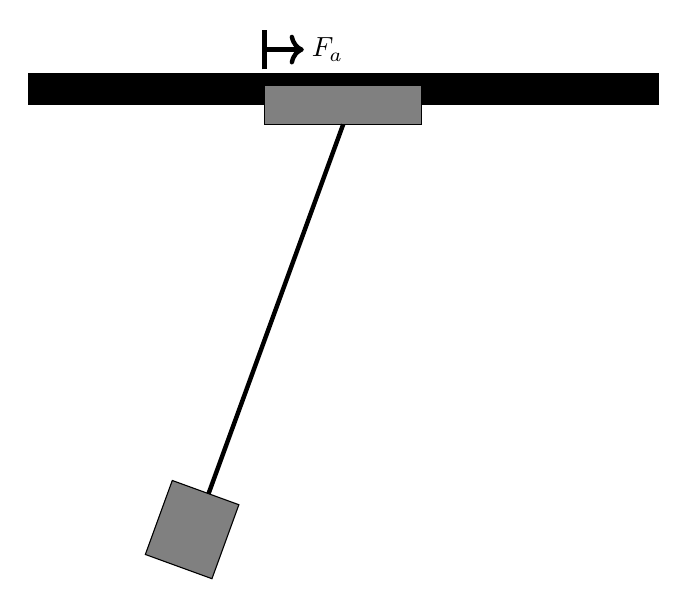
\begin{tikzpicture}
	\draw [ultra thick] (-1,0.7) -- (-1,1.2);
	\draw [->,ultra thick] (-1,0.95) -- (-0.5,0.95);
	\node at (-0.2,0.95) {$F_a$};
	%\node at (-2.32,-6.38) {$\Delta \theta$};
	

	\draw [fill = black] (-4,0.25) rectangle (4,0.65);
	\draw [fill = gray] (-1,0) rectangle (1,0.5);

	%\draw [dashed] (0,-0) -- (-1.07,-6.1); % 260
	\draw [ultra thick] (0,0) -- (-1.71,-4.69);  % 250
	%\draw [dashed] (0,0) -- (-3.1,-5.36);   % 240

	%\draw [<->,dashed] (-1.1,-6.17) arc [radius=6.2, start angle=260, end angle= 240];

	\draw[fill = gray,rotate around={-20:(-1.71,-4.69)}] (-2.2,-4.69) rectangle (-1.3,-5.69);
\end{tikzpicture}}}
    \end{itemize}                   
  \end{minipage}
  \end{frame}


%%%%%%%%%%%%%%%%%%%%%%%%%%%%%%%%%%%%%%%%%%% 

\begin{frame}{Introduktion}{Optimering af containerkraner}


 \begin{minipage}[t]{0.45\linewidth}
  \begin{itemize}
    \item<1-> Effektivitet af containerkraner 
        \begin{itemize}
          \item<1-> Der bliver fragtet 651 mio. container om året.
          \item<1-> Mere effektive kraner leder til mere overskud. 
        \end{itemize}
    \item<1-> Problemformulering
        \begin{itemize}
          \item<1-> \textit{"How can a control system be designed to automatically operate a crane."}
        \end{itemize}
  \end{itemize}
  \end{minipage}
  \begin{minipage}[t]{0.42\linewidth}
    \begin{itemize}
      \item<1->[] {
\scalebox{0.8}{
 \centering
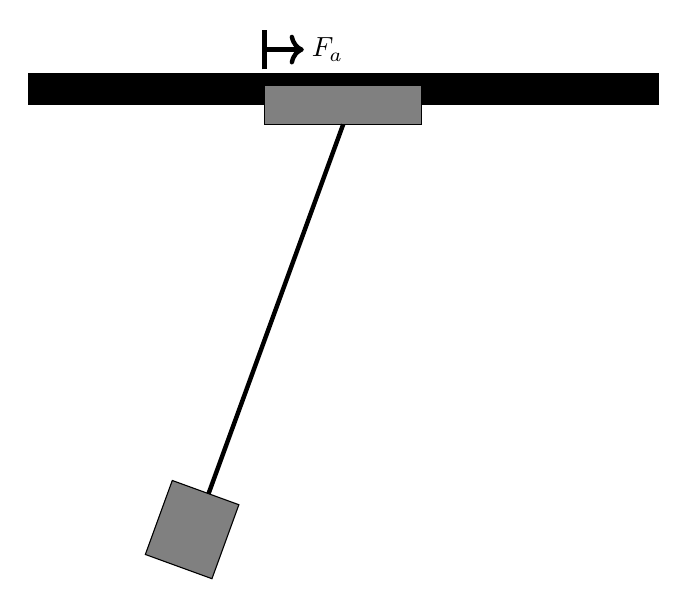
\begin{tikzpicture}
	\draw [ultra thick] (-1,0.7) -- (-1,1.2);
	\draw [->,ultra thick] (-1,0.95) -- (-0.5,0.95);
	\node at (-0.2,0.95) {$F_a$};
%	\node at (-2.32,-6.38) {$\Delta \theta$};
	

	\draw [fill = black] (-4,0.25) rectangle (4,0.65);
	\draw [fill = gray] (-1,0) rectangle (1,0.5);

%	\draw [dashed] (0,-0) -- (-1.07,-6.1); % 260
	\draw [ultra thick] (0,0) -- (-1.71,-4.69);  % 250%
%	\draw [dashed] (0,0) -- (-3.1,-5.36);   % 240

%	\draw [<->,dashed] (-1.1,-6.17) arc [radius=6.2, start angle=260, end angle= 240];

	\draw[fill = gray,rotate around={-20:(-1.71,-4.69)}] (-2.2,-4.69) rectangle (-1.3,-5.69);
\end{tikzpicture}}}
    \end{itemize}                   
  \end{minipage}
  \end{frame}


%%%%%%%%%%%%%%%%%%%%%%%%%%%%%%%%%%%%%%%%%%%%% 
\section{Opbygning af kran}
 \begin{frame}<beamer>
 \frametitle{Nicolaj Vinkel Christensen}
 \tableofcontents[currentsection]
 \end{frame}
\begin{frame}{Opbygning af kran}{Eksisterende setup}


 \begin{minipage}[H]{0.8\linewidth}
  \begin{itemize}
    \item<1-> Udgangspunkt i model kran 
        \begin{itemize}
          \item<1-> Eksisterende setup
              \begin{itemize}
              \item<1-> Trolley, elektromagnet, motor og gearing. 
              \item<1-> Sensore, effektforstærker forsyning. 
              \end{itemize}
        \end{itemize}
  \end{itemize}
  \end{minipage}
  \begin{minipage}[H]{0.6\linewidth}
    \begin{itemize}
      \item<1->[] {
              %\begin{figure}[H]
              %\centering
              %\end{figure}
              }
    \end{itemize}                   
  \end{minipage}
    \begin{center}
              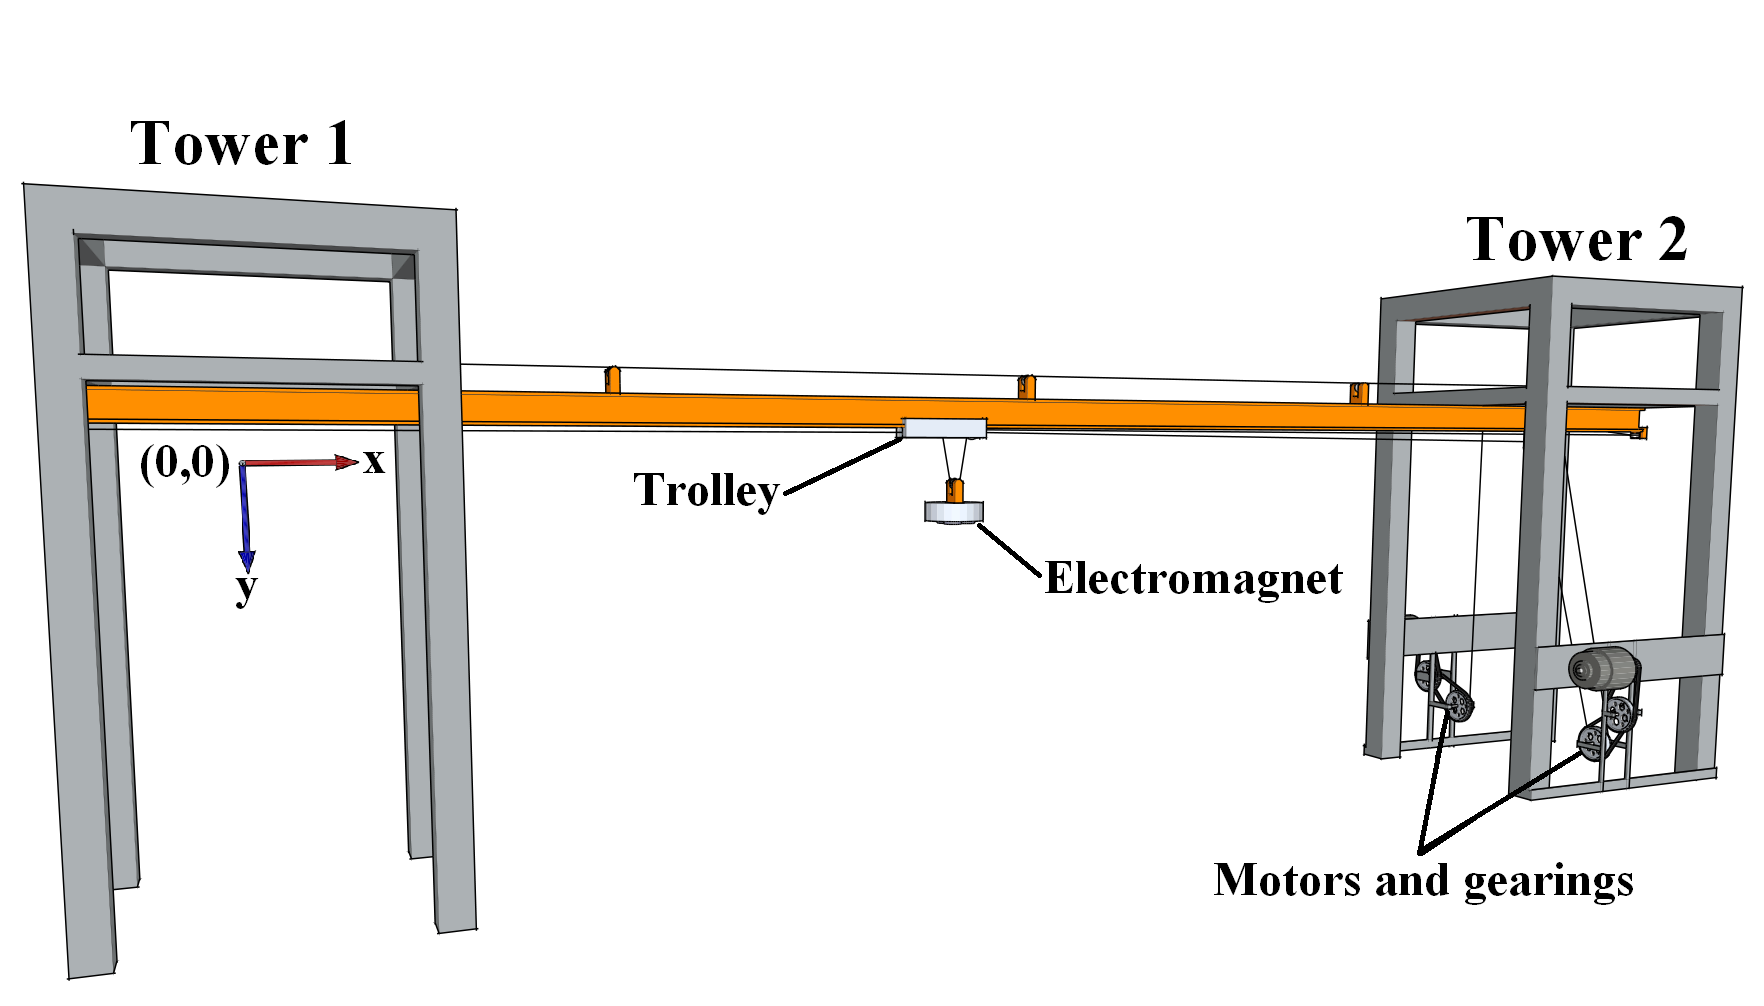
\includegraphics[width=0.8\textwidth]{Billeder/FullCrane}
    \end{center}
 \end{frame}

%%%%%%%%%%%%%%%%%%%%%%%%%%%%%%%%%%%%%%%%%%%%% 

\begin{frame}{Opbygning af kran}{Forbedringer af kranen}


 \begin{minipage}[H]{0.3\linewidth}
  \begin{itemize}
    \item<1-> Forbedringer 
    \vspace{0.2cm}
        \begin{itemize}
          \item<1-> Kontrol platform
          \vspace{0.2cm}
          \item<1-> Forsyning 
        \end{itemize}
  \end{itemize}
  \end{minipage}

  \vfill
  \begin{center}
  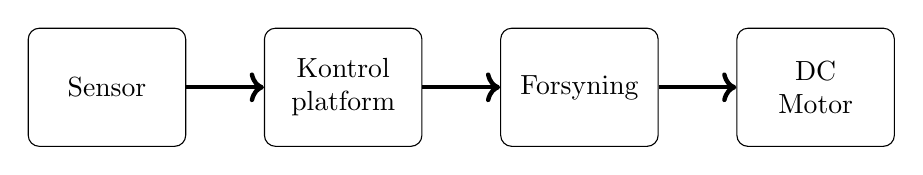
\begin{tikzpicture}

%Boxes
\node[fill = white,box] (Sensor) at (0,0) {Sensor};
\node[fill = white,box] (Con) at ($(3,0)+(Sensor)$) {Kontrol \\ platform};
\node[fill = white,box] (driv) at ($(3,0)+(Con)$) {Forsyning};
\node[fill = white,box] (Mot) at ($(3,0)+(driv)$) {DC \\ Motor};
%connections
\draw[->, ultra thick] (Sensor) -- (Con);
\draw[->, ultra thick] (Con) -- (driv);
\draw[->, ultra thick] (driv) -- (Mot);
\end{tikzpicture}%
\end{center}
  \end{frame}


  %%%%%%%%%%%%%%%%%%%%%%%%%%%%%%%%%%%%%%%%%%%%%%%%%%%%%

\begin{frame}{Opbygning af kran}{Forbedringer af kranen}


 \begin{minipage}[H]{0.3\linewidth}
  \begin{itemize}
    \item<1-> Forbedringer 
        \begin{itemize}
          \item<1-> Kontrol platform
            \begin{itemize}
              \item<1-> FPGA
              \item<1-> ADC
            \end{itemize}
          \item<1-> Forsyning 
            \begin{itemize}
              \item<1-> Motor drivere 
            \end{itemize}
          \item<1-> Fjernbetjening 
        \end{itemize}
  \end{itemize}
\end{minipage}

  \vfill

  \begin{center}
  \scalebox{0.8}{
  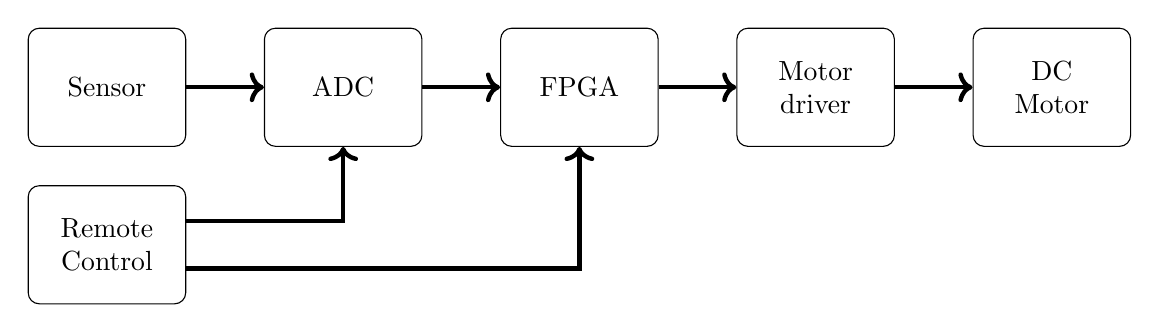
\begin{tikzpicture}
%Boxes
\node[fill = white,box] (Sensor) at (0,0) {Sensor};
\node[fill = white,box] (ADC) at ($(3,0)+(Sensor)$) {ADC};
\node[fill = white,box] (Con) at ($(3,0)+(ADC)$) {FPGA};
\node[fill = white,box] (driv) at ($(3,0)+(Con)$) {Motor \\ driver};
\node[fill = white,box] (Mot) at ($(3,0)+(driv)$) {DC \\ Motor};
\node[fill = white,box] (RC) at ($(0,-2)+(Sensor)$) {Remote \\ Control};
%connections
\draw[->, ultra thick] (Sensor) -- (ADC);
\draw[->, ultra thick] (ADC) -- (Con);
\draw[->, ultra thick] (Con) -- (driv);
\draw[->, ultra thick] (driv) -- (Mot);
\draw[->, ultra thick] ([yshift=0.3cm]RC.east) -| (ADC);
\draw[->, ultra thick] ([yshift=-0.3cm]RC.east) -| (Con);
\end{tikzpicture}}
\end{center}
  \end{frame}


  %%%%%%%%%%%%%%%%%%%%%%%%%%%%%%%%%%%%%%%%%%%%%%%%%%%%%

\begin{frame}{Opbygning af kran}{Forbedringer af kranen}

\begin{columns}[T]
\begin{column}{.35\textwidth}

  \begin{itemize}
    \item<1-> FPGA
        \begin{itemize}
          \item<1-> Papilio Duo
        \end{itemize}
    \vspace{0.8cm}
    \item<2-> Motor drivere
        \begin{itemize}
          \item<1-> Escon 50/5  
        \end{itemize}
    \vspace{0.8cm}
    \item<3-> ADC
        \begin{itemize}
          \item<1-> Papilio Analog Wing 
        \end{itemize}
  \end{itemize}
\end{column}%
\hfill%
\begin{column}{.65\textwidth}

\vspace{-0.7cm}
\begin{figure}[H]
  \centering
\onslide<1->  \begin{subfigure}{0.98\textwidth}
        \centering
        \includegraphics[width=0.5\textwidth]{Billeder/Papilio_DUO}
        \end{subfigure}
\onslide<2->  \begin{subfigure}{0.98\textwidth}
        \centering
        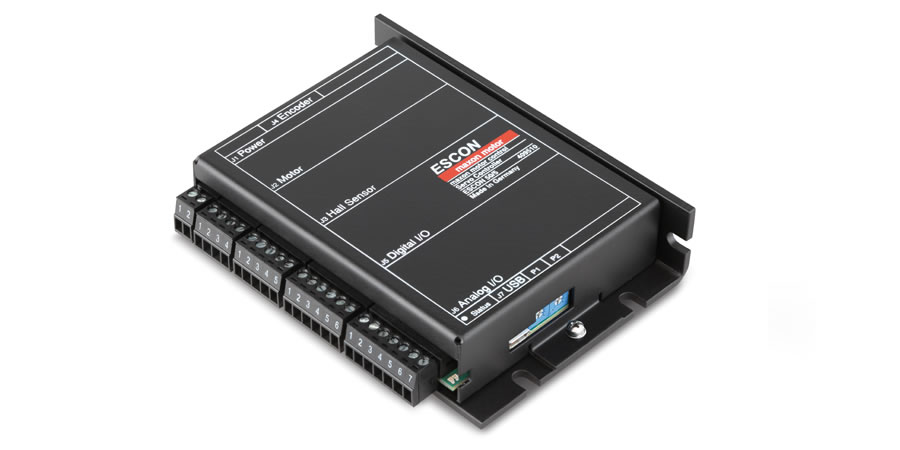
\includegraphics[width=0.5\textwidth]{Billeder/Escon_fig}
        \end{subfigure}
\onslide<3->  \begin{subfigure}{0.98\textwidth}
        \centering
        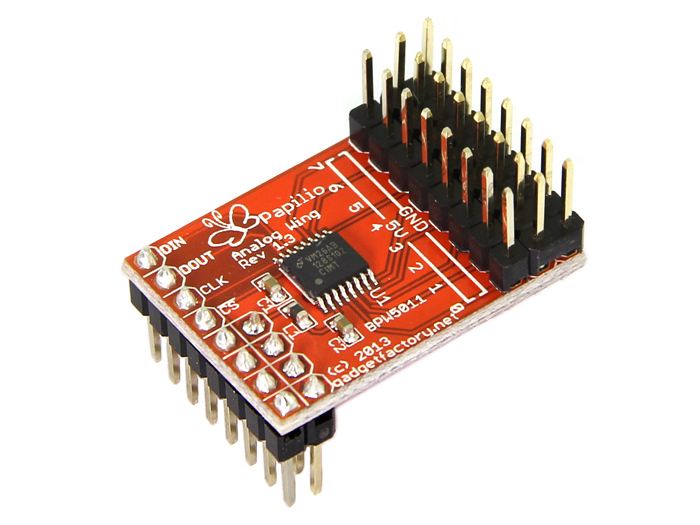
\includegraphics[width=0.5\textwidth]{Billeder/Analog_wing}
        \end{subfigure}     
\end{figure}

\end{column}
\end{columns}

  \end{frame}



%%%%%%%%%%%%%%%%%%%%%%%%%%%%%%%%%%%%%%% 
\section{Krav}
 \begin{frame}<beamer>
 \frametitle{Nicolaj Vinkel Christensen}
 \tableofcontents[currentsection]
 \end{frame}
\begin{frame}{Krav}{Hvordan skal kranen bevæge sig?}


 \begin{minipage}[H]{0.8\linewidth}
  \begin{itemize}
    \item<1-> Metoder: 
    \vspace{0.2cm}
        \begin{itemize}
          \item<1-> \textbf{(1)} Bevægelse i x- og y-aksen samtidig.
          \vspace{0.2cm}
          \item<1-> \textbf{(2)} Bevægelse i x- og y-aksen sekventielt.
        \end{itemize}
  \end{itemize}
  \end{minipage}

  \vfill
\begin{center}
\begin{figure}[H]
  \centering
  \begin{subfigure}[b]{.48\textwidth}
    \centering
      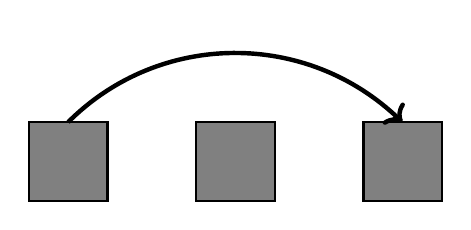
\begin{tikzpicture}
      \draw [fill=gray, thick](0,0) rectangle (1,1);
      \draw [fill=gray, thick](4.25,0) rectangle (5.25,1);
      \draw [fill=gray, thick](2.125,0) rectangle (3.125,1);

      \draw [->, ultra thick] (0.5,1) arc [radius=3, start angle=135, end angle= 45];
      \end{tikzpicture}
      \caption*{Metode \textbf{(1)}}
%    \hspace{-6cm}
  \end{subfigure}
  \begin{subfigure}[b]{.48\textwidth}
    \centering
        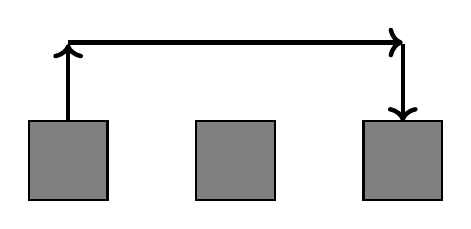
\begin{tikzpicture}
        \draw [fill=gray, thick](0,0) rectangle (1,1);
        \draw [fill=gray, thick](4.25,0) rectangle (5.25,1);
        \draw [fill=gray, thick](2.125,0) rectangle (3.125,1);

        \draw [->,ultra thick] (0.5,1) -- (0.5,1.98);
        \draw [->,ultra thick] (0.5,2) -- (4.75,2);
        \draw [->,ultra thick] (4.75,1.98) -- (4.75,1);
        \end{tikzpicture}
      \caption*{Metode \textbf{(2)}}
%    \hspace{6cm}
  \end{subfigure}
\end{figure}
\end{center}
  \end{frame}

%%%%%%%%%%%%%%%%%%%%%%%%%%%%%%%%%%%%%%% 
\begin{frame}{Krav}{Kravspecifikation}


 \begin{minipage}[H]{0.8\linewidth}
  \begin{itemize}
    \item<1-> Krav til de dynamiske egenskaber for kranen.
    \vspace{0.2cm}
        \begin{itemize}
          \item<1-> Opsat for positionen af elektromagneten. 
          \vspace{0.2cm}
          \item<1-> Opsat for x- og y-aksen individuelt.
        \end{itemize}
  \end{itemize}
  \end{minipage}
  \vfill
\begin{description}
    \item[\textbf{(A)}] : y-akse settling time for positiv retning , $t_s \leq 6,75 s$
    \item[\textbf{(B)}] : y-akse settling time for negativ retning, $t_s \leq 5,58 s$
    \item[\textbf{(C)}] : y-akse steady-state-error, $e_{ss} = 0,0\%$
    \item[\textbf{(D)}] : y-akse overshoot, $M_p = 0,0\%$ 
    \item[\textbf{(E)}] : x-akse settling time, $t_s \leq 17,45 s$
    \item[\textbf{(F)}] : x-akse steady-state-error, $e_{ss} = 0,0\%$ 
    \item[\textbf{(G)}] : x-akse overshoot, $M_p \leq 6,4\%$
\end{description}

  \end{frame}

%%%%%%%%%%%%%%%%
%\section{Model opstilling}
%%%%%%%%%%%% MID WAY AGENDA %%%%%%%%%%%%%%
\begin{frame}<beamer>
\frametitle{Daniel Bähner Andersen}
\tableofcontents[currentsection]
\end{frame}
%%%%%%%%%%%% MID WAY AGENDA %%%%%%%%%%%%%%


\subsection{Trolley- og pendulmodel}
\begin{frame}{Model opstilling}{Trolley- og pendulmodel}
  \begin{minipage}[t]{0.50\linewidth}
    \begin{itemize}
      	\item<1->[] {
              \begin{figure}[H]
              \centering
              \scalebox{0.75}{\input{Billeder/Daniel/mechanicalSystem.ralf}}
              \end{figure}}
        \item<3->[] {
     		\begin{equation*}
				m_t \ddot{x} = F_a - F_{sx_p} - F_{Bt} = F_a - F_s \cdot \sin(\theta) - B_t\dot{x}
			\end{equation*}}      
    \end{itemize}           
  \end{minipage}
  \begin{minipage}[t]{0.45\linewidth}
\bigskip
\bigskip 
\bigskip
	\begin{itemize}
    	\item<2->[] Fritlegeme diagram for trolley  
	\end{itemize}    
\medskip 
    \begin{itemize}            
	\item<2->[] {
              \begin{figure}[H]
              \centering
              \scalebox{0.75}{\input{Billeder/Daniel/FBDtrolley.ralf}}
              \end{figure}}	     	
    \end{itemize}           
  \end{minipage}
\end{frame} 
%%%%%%%%%%%%%%%%

\begin{frame}{Model opstilling}{Trolley- og pendulmodel}
  \begin{minipage}[t]{0.50\linewidth}
    \begin{itemize}
      	\item<1->[] {
              \begin{figure}[H]
              \centering
              \scalebox{0.75}{\input{Billeder/Daniel/mechanicalSystem.ralf}}
              \end{figure}}
        \item<3->[] {
     		\begin{equation*}
				m_L \ddot{x_L} = m_L(\ddot{x} - \ddot{x_p}) =  F_{sx_p} + F_{Bx_p} = F_s \cdot \sin(\theta) + \frac{1}{L} B_p \dot{\theta} \cos(\theta)
			\end{equation*}} 
		\item<4->[] {
     		\begin{equation*}
				x_p = \sin(\theta) \cdot L \Rightarrow \ddot{x_p} = -\sin(\theta)\cdot \dot{\theta}^2 \cdot L + \cos(\theta)\cdot \ddot{\theta} \cdot L
			\end{equation*}}  	     
    \end{itemize}           
  \end{minipage}
  \begin{minipage}[t]{0.45\linewidth}
\bigskip
\bigskip 
\bigskip
	\begin{itemize}
    	\item<2->[] Fritlegeme diagram for pendulet i x-aksen  
	\end{itemize}    
\medskip 
    \begin{itemize}            
	\item<2->[] {
              \begin{figure}[H]
              \centering
              \scalebox{0.75}{\input{Billeder/Daniel/FBDPenX.ralf}}
              \end{figure}}	     	
    \end{itemize}           
  \end{minipage}
\end{frame} 
%%%%%%%%%%%%%%%%

\begin{frame}{Model opstilling}{Trolley- og pendulmodel}
  \begin{minipage}[t]{0.50\linewidth}
    \begin{itemize}
      	\item<1->[] {
              \begin{figure}[H]
              \centering
              \scalebox{0.75}{\input{Billeder/Daniel/mechanicalSystem.ralf}}
              \end{figure}}
        \item<3->[] {
     		\begin{equation*}
				m_L \ddot{y} =  F_{By_p} + F_g - F_{sy_p}  = \frac{1}{L} B_p \dot{\theta} \sin(\theta) + F_g - F_s \cdot \cos(\theta)
			\end{equation*}}
		\item<4->[] {
     		\begin{equation*}
				y = \cos(\theta) \cdot L \Rightarrow \ddot{y} = -\cos(\theta) \cdot \dot{\theta}^2 \cdot L - \sin(\theta) \cdot \ddot{\theta} \cdot L
			\end{equation*}}  	      
    \end{itemize}           
  \end{minipage}
  \begin{minipage}[t]{0.45\linewidth}
\bigskip
\bigskip 
\bigskip
	\begin{itemize}
    	\item<2->[] Fritlegeme diagram for pendulet i y-aksen  
	\end{itemize}    
\medskip 
    \begin{itemize}            
	\item<2->[] {
              \begin{figure}[H]
              \centering
              \scalebox{0.75}{\input{Billeder/Daniel/FBDPenY.ralf}}
              \end{figure}}	     	
    \end{itemize}           
  \end{minipage}
\end{frame} 
%%%%%%%%%%%%%%%%
% Resulterende modeller
%%%%%%%%%%%%%%%%

\begin{frame}{Model opstilling}{Trolley- og pendulmodel}
    \begin{itemize}
      	\item<1-> Overføringsfunktioner 
      	\begin{itemize}
      		\item<2-> Lineariseret 
      		\item<2-> Laplace tranformeret  
      	\end{itemize}	       
    \end{itemize}  
\bigskip
\bigskip             
  \begin{minipage}[t]{0.3\linewidth} 
    \begin{itemize}            
	\item<3->[] {\begin{equation*}
             		\frac{X(s)}{F_a(s)}   
                \end{equation*}}	
    \end{itemize}           
  \end{minipage}
  \begin{minipage}[t]{0.3\linewidth} 
    \begin{itemize}            
	\item<4->[] {\begin{equation*}
             		\frac{\Theta(s)}{F_a(s)} 
                \end{equation*}}	
    \end{itemize}           
  \end{minipage}
  \begin{minipage}[t]{0.3\linewidth} 
    \begin{itemize}            
	\item<5->[] {\begin{equation*}
             		\frac{X_L(s)}{F_a(s)}  
                \end{equation*}}	
    \end{itemize}           
  \end{minipage}

%%%%%%%%%%%%%%%%

\end{frame}
\begin{frame}{Model opstilling}{Trolley- og pendulmodel}
  \begin{minipage}[t]{0.48\linewidth}
    \begin{itemize}
      	\item<1->[] {
              \begin{figure}[H]
              \centering
              % This file was created by matlab2tikz.
%
%The latest updates can be retrieved from
%  http://www.mathworks.com/matlabcentral/fileexchange/22022-matlab2tikz-matlab2tikz
%where you can also make suggestions and rate matlab2tikz.
%
\definecolor{mycolor3}{rgb}{1.00000,0.00000,1.00000}%
%
\begin{tikzpicture}

\begin{axis}[%
width=0.75\textwidth,
height=0.6\textwidth,
scale only axis,
separate axis lines,
every outer x axis line/.append style={white!40!black},
every x tick label/.append style={font=\color{white!40!black}},
xmin=0,
xmax=3,
xmajorgrids,
xlabel={Time [s]},
every outer y axis line/.append style={white!40!black},
every y tick label/.append style={font=\color{white!40!black}},
ymin=0,
ymax=4,
ymajorgrids,
ylabel={Position [m]},
axis background/.style={fill=white},
%legend style={at={(0.97,0.03)},anchor=south east,legend cell align=left,align=left,draw=black}
]
\addplot [color=blue,dashed]
  table[row sep=crcr]{%
0	0\\
0.0198000198000198	0.000117371982093649\\
0.0396000396000396	0.000467198587515959\\
0.0594000594000594	0.00104592099734742\\
0.0792000792000792	0.00184983314546589\\
0.099000099000099	0.00287510691776669\\
0.118800118800119	0.00411781840981444\\
0.138600138600139	0.00557397474629027\\
0.158400158400158	0.00723954098599551\\
0.178200178200178	0.00911046666309538\\
0.198000198000198	0.011182711547912\\
0.217800217800218	0.0134522702480346\\
0.237600237600238	0.0159151953119145\\
0.257400257400257	0.0185676185415437\\
0.277200277200277	0.0214057702673806\\
0.297000297000297	0.0244259963865006\\
0.316800316800317	0.0276247730131596\\
0.336600336600337	0.0309987186387668\\
0.356400356400356	0.0345446037449006\\
0.376200376200376	0.0382593578578044\\
0.396000396000396	0.0421400740751169\\
0.415800415800416	0.0461840111349201\\
0.435600435600436	0.0503885931330279\\
0.455400455400455	0.0547514070264512\\
0.475200475200475	0.0592701980888335\\
0.495000495000495	0.0639428635071779\\
0.514800514800515	0.0687674443282327\\
0.534600534600535	0.0737421159774428\\
0.554400554400554	0.0788651775834247\\
0.574200574200574	0.0841350403465974\\
0.594000594000594	0.0895502151920606\\
0.613800613800614	0.0951092999442825\\
0.633600633600634	0.100810966254923\\
0.653400653400653	0.106653946505489\\
0.673200673200673	0.112637020893866\\
0.693000693000693	0.118759004898454\\
0.712800712800713	0.125018737296104\\
0.732600732600733	0.131415068890667\\
0.752400752400752	0.137946852088214\\
0.772200772200772	0.14461293143322\\
0.792000792000792	0.1514121351977\\
0.811800811800812	0.158343268092783\\
0.831600831600832	0.165405105149925\\
0.851400851400851	0.17259638679724\\
0.871200871200871	0.179915815135537\\
0.891000891000891	0.187362051398984\\
0.910800910800911	0.194933714567001\\
0.930600930600931	0.202629381077348\\
0.95040095040095	0.210447585575473\\
0.97020097020097	0.218386822622299\\
0.99000099000099	0.226445549271692\\
1.00980100980101	0.234622188420048\\
1.02960102960103	0.242915132823749\\
1.04940104940105	0.25132274967559\\
1.06920106920107	0.259843385628732\\
1.08900108900109	0.26847537215609\\
1.10880110880111	0.277217031134356\\
1.12860112860113	0.286066680544765\\
1.14840114840115	0.295022640187317\\
1.16820116820117	0.304083237311067\\
1.18800118800119	0.313246812070327\\
1.20780120780121	0.322511722724789\\
1.22760122760123	0.331876350510696\\
1.24740124740125	0.341339104119852\\
1.26720126720127	0.350898423733452\\
1.28700128700129	0.360552784568118\\
1.30680130680131	0.370300699902026\\
1.32660132660133	0.380140723559401\\
1.34640134640135	0.390071451841778\\
1.36620136620137	0.400091524904155\\
1.38600138600139	0.410199627583343\\
1.40580140580141	0.420394489694282\\
1.42560142560143	0.430674885817913\\
1.44540144540145	0.441039634611024\\
1.46520146520147	0.451487597674545\\
1.48500148500149	0.462017678021794\\
1.5048015048015	0.472628818192252\\
1.52460152460152	0.483319998059567\\
1.54440154440154	0.49409023238456\\
1.56420156420156	0.504938568165243\\
1.58400158400158	0.515864081836034\\
1.6038016038016	0.52686587636783\\
1.62360162360162	0.537943078319116\\
1.64340164340164	0.549094834886185\\
1.66320166320166	0.560320310997745\\
1.68300168300168	0.571618686495795\\
1.7028017028017	0.582989153440829\\
1.72260172260172	0.594430913575186\\
1.74240174240174	0.605943175973792\\
1.76220176220176	0.617525154906857\\
1.78200178200178	0.62917606793415\\
1.8018018018018	0.640895134245664\\
1.82160182160182	0.652681573258549\\
1.84140184140184	0.664534603475566\\
1.86120186120186	0.676453441605695\\
1.88100188100188	0.688437301943348\\
1.9008019008019	0.700485395998615\\
1.92060192060192	0.712596932367409\\
1.94040194040194	0.724771116827157\\
1.96020196020196	0.737007152640892\\
1.98000198000198	0.749304241050275\\
1.999801999802	0.761661581936187\\
2.01960201960202	0.774078374624081\\
2.03940203940204	0.786553818810351\\
2.05920205920206	0.799087115585408\\
2.07900207900208	0.811677468529066\\
2.0988020988021	0.824324084854138\\
2.11860211860212	0.837026176574811\\
2.13840213840214	0.849782961677379\\
2.15820215820216	0.862593665272231\\
2.17800217800218	0.875457520707578\\
2.1978021978022	0.888373770627184\\
2.21760221760222	0.901341667956384\\
2.23740223740224	0.914360476802757\\
2.25720225720226	0.927429473260074\\
2.27700227700228	0.94054794610638\\
2.2968022968023	0.953715197389376\\
2.31660231660232	0.966930542894512\\
2.33640233640234	0.98019331249341\\
2.35620235620236	0.993502850372339\\
2.37600237600238	1.00685851514245\\
2.3958023958024	1.02025967983534\\
2.41560241560242	1.03370573178913\\
2.43540243540244	1.0471960724318\\
2.45520245520246	1.06073011696986\\
2.47500247500248	1.07430729399124\\
2.49480249480249	1.08792704499263\\
2.51460251460251	1.10158882384169\\
2.53440253440253	1.11529209618533\\
2.55420255420255	1.12903633881526\\
2.57400257400257	1.14282103900231\\
2.59380259380259	1.15664569381055\\
2.61360261360261	1.17050980940226\\
2.63340263340263	1.18441290034412\\
2.65320265320265	1.19835448892432\\
2.67300267300267	1.21233410448979\\
2.69280269280269	1.22635128281168\\
2.71260271260271	1.24040556548637\\
2.73240273240273	1.25449649937836\\
2.75220275220275	1.26862363611018\\
2.77200277200277	1.28278653160369\\
2.79180279180279	1.29698474567574\\
2.81160281160281	1.31121784169037\\
2.83140283140283	1.32548538626855\\
2.85120285120285	1.33978694905556\\
2.87100287100287	1.35412210254516\\
2.89080289080289	1.36849042195882\\
2.91060291060291	1.38289148517758\\
2.93040293040293	1.39732487272328\\
2.95020295020295	1.41179016778545\\
2.97000297000297	1.42628695628955\\
2.98980298980299	1.44081482700188\\
3.00960300960301	1.45537337166625\\
3.02940302940303	1.46996218516703\\
3.04920304920305	1.48458086571351\\
3.06900306900307	1.49922901504009\\
3.08880308880309	1.51390623861714\\
3.10860310860311	1.52861214586738\\
3.12840312840313	1.54334635038295\\
3.14820314820315	1.55810847013859\\
3.16800316800317	1.57289812769669\\
3.18780318780319	1.5877149504004\\
3.20760320760321	1.60255857055129\\
3.22740322740323	1.61742862556883\\
3.24720324720325	1.63232475812905\\
3.26700326700327	1.64724661628051\\
3.28680328680329	1.66219385353608\\
3.30660330660331	1.67716612893961\\
3.32640332640333	1.69216310710698\\
3.34620334620335	1.70718445824142\\
3.36600336600337	1.72222985812363\\
3.38580338580339	1.73729898807739\\
3.40560340560341	1.75239153491187\\
3.42540342540343	1.76750719084206\\
3.44520344520345	1.78264565338915\\
3.46500346500346	1.7978066252628\\
3.48480348480348	1.81298981422748\\
3.5046035046035	1.82819493295522\\
3.52440352440352	1.84342169886712\\
3.54420354420354	1.8586698339662\\
3.56400356400356	1.8739390646639\\
3.58380358380358	1.88922912160276\\
3.6036036036036	1.90453973947765\\
3.62340362340362	1.91987065685775\\
3.64320364320364	1.93522161601138\\
3.66300366300366	1.95059236273578\\
3.68280368280368	1.96598264619338\\
3.7026037026037	1.98139221875631\\
3.72240372240372	1.99682083586045\\
3.74220374220374	2.01226825587013\\
3.76200376200376	2.02773423995431\\
3.78180378180378	2.04321855197505\\
3.8016038016038	2.0587209583886\\
3.82140382140382	2.0742412281593\\
3.84120384120384	2.08977913268635\\
3.86100386100386	2.10533444574324\\
3.88080388080388	2.12090694342945\\
3.9006039006039	2.13649640413378\\
3.92040392040392	2.15210260850874\\
3.94020394020394	2.16772533945509\\
3.96000396000396	2.18336438211558\\
3.97980397980398	2.1990195238769\\
3.999603999604	2.21469055437873\\
4.01940401940402	2.23037726552871\\
4.03920403920404	2.24607945152233\\
4.05900405900406	2.26179690886628\\
4.07880407880408	2.27752943640452\\
4.0986040986041	2.29327683534552\\
4.11840411840412	2.30903890929006\\
4.13820413820414	2.32481546425816\\
4.15800415800416	2.34060630871458\\
4.17780417780418	2.35641125359182\\
4.1976041976042	2.37223011231005\\
4.21740421740422	2.38806270079317\\
4.23720423720424	2.40390883748065\\
4.25700425700426	2.41976834333455\\
4.27680427680428	2.43564104184156\\
4.2966042966043	2.45152675900974\\
4.31640431640432	2.46742532335995\\
4.33620433620434	2.48333656591189\\
4.35600435600436	2.49926032016485\\
4.37580437580438	2.51519642207341\\
4.3956043956044	2.53114471001826\\
4.41540441540442	2.54710502477257\\
4.43520443520443	2.56307720946409\\
4.45500445500446	2.5790611095337\\
4.47480447480447	2.59505657269068\\
4.49460449460449	2.61106344886515\\
4.51440451440451	2.6270815901585\\
4.53420453420453	2.64311085079199\\
4.55400455400455	2.65915108705431\\
4.57380457380457	2.67520215724847\\
4.59360459360459	2.69126392163861\\
4.61340461340461	2.70733624239726\\
4.63320463320463	2.7234189835533\\
4.65300465300465	2.73951201094136\\
4.67280467280467	2.7556151921527\\
4.69260469260469	2.77172839648818\\
4.71240471240471	2.78785149491345\\
4.73220473220473	2.80398436001666\\
4.75200475200475	2.82012686596883\\
4.77180477180477	2.8362788884871\\
4.79160479160479	2.85244030480089\\
4.81140481140481	2.86861099362098\\
4.83120483120483	2.88479083511161\\
4.85100485100485	2.90097971086542\\
4.87080487080487	2.91717750388126\\
4.89060489060489	2.93338409854467\\
4.91040491040491	2.94959938061088\\
4.93020493020493	2.9658232371902\\
4.95000495000495	2.98205555673549\\
4.96980496980497	2.99829622903159\\
4.98960498960499	3.01454514518643\\
5.00940500940501	3.03080219762353\\
5.02920502920503	3.04706728007565\\
5.04900504900505	3.06334028757945\\
5.06880506880507	3.07962111647071\\
5.08860508860509	3.09590966438\\
5.10840510840511	3.11220583022862\\
5.12820512820513	3.12850951422437\\
5.14800514800515	3.14482061785725\\
5.16780516780517	3.1611390438946\\
5.18760518760519	3.17746469637581\\
5.20740520740521	3.19379748060623\\
5.22720522720523	3.21013730315026\\
5.24700524700525	3.22648407182363\\
5.26680526680527	3.24283769568455\\
5.28660528660529	3.25919808502393\\
5.30640530640531	3.27556515135455\\
5.32620532620533	3.29193880739913\\
5.34600534600535	3.30831896707737\\
5.36580536580537	3.3247055454921\\
5.38560538560538	3.34109845891434\\
5.40540540540541	3.35749762476761\\
5.42520542520542	3.37390296161138\\
5.44500544500545	3.3903143891239\\
5.46480546480546	3.40673182808435\\
5.48460548460548	3.42315520035462\\
5.5044055044055	3.4395844288606\\
5.52420552420552	3.45601943757333\\
5.54400554400554	3.47246015148991\\
5.56380556380556	3.4889064966145\\
5.58360558360558	3.50535839993925\\
5.6034056034056	3.52181578942558\\
5.62320562320562	3.53827859398563\\
5.64300564300564	3.55474674346415\\
5.66280566280566	3.5712201686208\\
5.68260568260568	3.587698801113\\
5.7024057024057	3.60418257347938\\
5.72220572220572	3.62067141912383\\
5.74200574200574	3.63716527230027\\
5.76180576180576	3.6536640680981\\
5.78160578160578	3.67016774242837\\
5.8014058014058	3.6866762320107\\
5.82120582120582	3.70318947436088\\
5.84100584100584	3.71970740777926\\
5.86080586080586	3.73622997133976\\
5.88060588060588	3.75275710487959\\
5.9004059004059	3.76928874898955\\
5.92020592020592	3.785824845005\\
5.94000594000594	3.80236533499726\\
5.95980595980596	3.81891016176561\\
5.97960597960598	3.83545926882962\\
5.999405999406	3.85201260042196\\
6.01920601920602	3.86857010148144\\
6.03900603900604	3.88513171764642\\
6.05880605880606	3.9016973952483\\
6.07860607860608	3.91826708130533\\
6.0984060984061	3.93484072351637\\
6.11820611820612	3.95141827025483\\
6.13800613800614	3.96799967056255\\
6.15780615780616	3.9845848741437\\
6.17760617760618	4.00117383135858\\
};
%\addlegendentry{1A model};

\addplot [color=mycolor3,dashed]
  table[row sep=crcr]{%
0	0\\
0.0198000198000198	0.000227892410235163\\
0.0396000396000396	0.00090712459880352\\
0.0594000594000594	0.00203078667284401\\
0.0792000792000792	0.00359168284060122\\
0.099000099000099	0.00558238033886875\\
0.118800118800119	0.0079952604155103\\
0.138600138600139	0.0108225704027772\\
0.158400158400158	0.014056475956744\\
0.178200178200178	0.0176891125904591\\
0.198000198000198	0.021712635691752\\
0.217800217800218	0.0261192682893718\\
0.237600237600238	0.0309013459115112\\
0.257400257400257	0.0360513579670428\\
0.277200277200277	0.0415619851702028\\
0.297000297000297	0.0474261326222946\\
0.316800316800317	0.0536369582575948\\
0.336600336600337	0.0601878964534626\\
0.356400356400356	0.0670726766952162\\
0.376200376200376	0.0742853372733187\\
0.396000396000396	0.0818202340725941\\
0.415800415800416	0.0896720445895411\\
0.435600435600436	0.0978357673834158\\
0.455400455400455	0.106306717228894\\
0.475200475200475	0.115080516292232\\
0.495000495000495	0.124153081698509\\
0.514800514800515	0.133520609894525\\
0.534600534600535	0.143179558240157\\
0.554400554400554	0.153126624280491\\
0.574200574200574	0.16335872316206\\
0.594000594000594	0.173872963659361\\
0.613800613800614	0.184666623272901\\
0.633600633600634	0.195737122847933\\
0.653400653400653	0.207082001144318\\
0.673200673200673	0.218698889763406\\
0.693000693000693	0.230585488808087\\
0.712800712800713	0.242739543618113\\
0.732600732600733	0.255158822885164\\
0.752400752400752	0.267841098411829\\
0.772200772200772	0.280784126736427\\
0.792000792000792	0.293985632802253\\
0.811800811800812	0.307443295806191\\
0.831600831600832	0.321154737318324\\
0.851400851400851	0.335117511722005\\
0.871200871200871	0.349329098983326\\
0.891000891000891	0.363786899720672\\
0.910800910800911	0.378488232509544\\
0.930600930600931	0.393430333325475\\
0.95040095040095	0.40861035699899\\
0.97020097020097	0.42402538053149\\
0.99000099000099	0.439672408099714\\
1.00980100980101	0.455548377559404\\
1.02960102960103	0.471650168245682\\
1.04940104940105	0.487974609858768\\
1.06920106920107	0.504518492218601\\
1.08900108900109	0.521278575670779\\
1.10880110880111	0.538251601928625\\
1.12860112860113	0.555434305141945\\
1.14840114840115	0.572823422991905\\
1.16820116820117	0.590415707622949\\
1.18800118800119	0.608207936236687\\
1.20780120780121	0.6261969211886\\
1.22760122760123	0.644379519446017\\
1.24740124740125	0.662752641284681\\
1.26720126720127	0.681313258120932\\
1.28700128700129	0.700058409396782\\
1.30680130680131	0.718985208455524\\
1.32660132660133	0.738090847365678\\
1.34640134640135	0.757372600670785\\
1.36620136620137	0.776827828061388\\
1.38600138600139	0.796453975983356\\
1.40580140580141	0.816248578213241\\
1.42560142560143	0.836209255446392\\
1.44540144540145	0.856333713956937\\
1.46520146520147	0.876619743400438\\
1.48500148500149	0.897065213839795\\
1.5048015048015	0.91766807208291\\
1.52460152460152	0.938426337426644\\
1.54440154440154	0.959338096905681\\
1.56420156420156	0.980401500147244\\
1.58400158400158	1.00161475393304\\
1.6038016038016	1.02297611656865\\
1.62360162360162	1.04448389215794\\
1.64340164340164	1.06613642487565\\
1.66320166320166	1.08793209332623\\
1.68300168300168	1.10986930507015\\
1.7028017028017	1.13194649139163\\
1.72260172260172	1.1541621023734\\
1.74240174240174	1.17651460233531\\
1.76220176220176	1.19900246568453\\
1.78200178200178	1.22162417321531\\
1.8018018018018	1.24437820888717\\
1.82160182160182	1.26726305710072\\
1.84140184140184	1.29027720048113\\
1.86120186120186	1.31341911817074\\
1.88100188100188	1.33668728462371\\
1.9008019008019	1.36008016888806\\
1.92060192060192	1.38359623435361\\
1.94040194040194	1.4072339389377\\
1.96020196020196	1.43099173567569\\
1.98000198000198	1.45486807367817\\
1.999801999802	1.47886139941362\\
2.01960201960202	1.50297015827207\\
2.03940203940204	1.5271927963638\\
2.05920205920206	1.55152776250574\\
2.07900207900208	1.57597351034828\\
2.0988020988021	1.60052850059579\\
2.11860211860212	1.62519120327506\\
2.13840213840214	1.6499601000085\\
2.15820215820216	1.67483368625082\\
2.17800217800218	1.69981047345153\\
2.1978021978022	1.72488899110858\\
2.21760221760222	1.7500677886829\\
2.23740223740224	1.77534543734716\\
2.25720225720226	1.8007205315467\\
2.27700227700228	1.82619169035497\\
2.2968022968023	1.85175755861014\\
2.31660231660232	1.87741680782392\\
2.33640233640234	1.90316813685809\\
2.35620235620236	1.92901027236812\\
2.37600237600238	1.9549419690172\\
2.3958023958024	1.98096200946761\\
2.41560241560242	2.00706920415952\\
2.43540243540244	2.03326239089041\\
2.45520245520246	2.05954043421038\\
2.47500247500248	2.08590222465133\\
2.49480249480249	2.11234667780909\\
2.51460251460251	2.13887273329931\\
2.53440253440253	2.16547935360848\\
2.55420255420255	2.19216552286217\\
2.57400257400257	2.21893024553244\\
2.59380259380259	2.24577254510615\\
2.61360261360261	2.27269146273552\\
2.63340263340263	2.2996860558909\\
2.65320265320265	2.32675539703496\\
2.67300267300267	2.35389857233581\\
2.69280269280269	2.38111468043496\\
2.71260271260271	2.40840283128434\\
2.73240273240273	2.43576214506458\\
2.75220275220275	2.46319175119466\\
2.77200277200277	2.49069078744123\\
2.79180279180279	2.51825839913354\\
};
%\addlegendentry{2A model};

\addplot [color=blue,solid]
  table[row sep=crcr]{%
0	-0.00109999999999999\\
0.0198000198000198	5.55111512312578e-17\\
0.0396000396000396	0.00110000000000005\\
0.0594000594000594	0.00330000000000003\\
0.0792000792000792	0.00440000000000002\\
0.099000099000099	0.00660000000000005\\
0.118800118800119	0.00880000000000003\\
0.138600138600139	0.00990000000000002\\
0.158400158400158	0.0121000000000001\\
0.178200178200178	0.0132\\
0.198000198000198	0.0154\\
0.217800217800218	0.0187000000000001\\
0.237600237600238	0.0198\\
0.257400257400257	0.022\\
0.277200277200277	0.0242000000000001\\
0.297000297000297	0.0264\\
0.316800316800317	0.0275\\
0.336600336600337	0.0308000000000001\\
0.356400356400356	0.0341\\
0.376200376200376	0.0374\\
0.396000396000396	0.0396\\
0.415800415800416	0.0429\\
0.435600435600436	0.0473\\
0.455400455400455	0.0484000000000001\\
0.475200475200475	0.0539000000000001\\
0.495000495000495	0.0572\\
0.514800514800515	0.0605000000000001\\
0.534600534600535	0.0660000000000001\\
0.554400554400554	0.0693\\
0.574200574200574	0.0726000000000001\\
0.594000594000594	0.0737\\
0.613800613800614	0.0781000000000001\\
0.633600633600634	0.0825\\
0.653400653400653	0.0858\\
0.673200673200673	0.0902000000000001\\
0.693000693000693	0.0946\\
0.712800712800713	0.1001\\
0.732600732600733	0.1034\\
0.752400752400752	0.1089\\
0.772200772200772	0.1133\\
0.792000792000792	0.1177\\
0.811800811800812	0.1232\\
0.831600831600832	0.1276\\
0.851400851400851	0.1331\\
0.871200871200871	0.1375\\
0.891000891000891	0.1441\\
0.910800910800911	0.1485\\
0.930600930600931	0.154\\
0.95040095040095	0.1595\\
0.97020097020097	0.165\\
0.99000099000099	0.1705\\
1.00980100980101	0.1771\\
1.02960102960103	0.1826\\
1.04940104940105	0.1892\\
1.06920106920107	0.1958\\
1.08900108900109	0.2013\\
1.10880110880111	0.2079\\
1.12860112860113	0.2145\\
1.14840114840115	0.2211\\
1.16820116820117	0.2277\\
1.18800118800119	0.2332\\
1.20780120780121	0.2409\\
1.22760122760123	0.2464\\
1.24740124740125	0.2541\\
1.26720126720127	0.2618\\
1.28700128700129	0.2684\\
1.30680130680131	0.2761\\
1.32660132660133	0.2849\\
1.34640134640135	0.2926\\
1.36620136620137	0.2992\\
1.38600138600139	0.3069\\
1.40580140580141	0.3146\\
1.42560142560143	0.3234\\
1.44540144540145	0.3311\\
1.46520146520147	0.3399\\
1.48500148500149	0.3476\\
1.5048015048015	0.3564\\
1.52460152460152	0.3652\\
1.54440154440154	0.3729\\
1.56420156420156	0.3817\\
1.58400158400158	0.3938\\
1.6038016038016	0.4026\\
1.62360162360162	0.4103\\
1.64340164340164	0.4191\\
1.66320166320166	0.4268\\
1.68300168300168	0.4356\\
1.7028017028017	0.4532\\
1.72260172260172	0.4521\\
1.74240174240174	0.4609\\
1.76220176220176	0.4697\\
1.78200178200178	0.4785\\
1.8018018018018	0.4873\\
1.82160182160182	0.4961\\
1.84140184140184	0.5049\\
1.86120186120186	0.5137\\
1.88100188100188	0.5225\\
1.9008019008019	0.5313\\
1.92060192060192	0.5412\\
1.94040194040194	0.5456\\
1.96020196020196	0.5555\\
1.98000198000198	0.5643\\
1.999801999802	0.5742\\
2.01960201960202	0.583\\
2.03940203940204	0.5918\\
2.05920205920206	0.6017\\
2.07900207900208	0.6127\\
2.0988020988021	0.6215\\
2.11860211860212	0.6325\\
2.13840213840214	0.6424\\
2.15820215820216	0.6534\\
2.17800217800218	0.6622\\
2.1978021978022	0.6732\\
2.21760221760222	0.6842\\
2.23740223740224	0.693\\
2.25720225720226	0.7051\\
2.27700227700228	0.7161\\
2.2968022968023	0.726\\
2.31660231660232	0.737\\
2.33640233640234	0.748\\
2.35620235620236	0.759\\
2.37600237600238	0.77\\
2.3958023958024	0.781\\
2.41560241560242	0.792\\
2.43540243540244	0.803\\
2.45520245520246	0.8151\\
2.47500247500248	0.8261\\
2.49480249480249	0.8371\\
2.51460251460251	0.8481\\
2.53440253440253	0.8624\\
2.55420255420255	0.8734\\
2.57400257400257	0.8844\\
2.59380259380259	0.8954\\
2.61360261360261	0.9064\\
2.63340263340263	0.9174\\
2.65320265320265	0.9284\\
2.67300267300267	0.9394\\
2.69280269280269	0.9515\\
2.71260271260271	0.9625\\
2.73240273240273	0.9735\\
2.75220275220275	0.9845\\
2.77200277200277	0.9922\\
2.79180279180279	1.0043\\
2.81160281160281	1.0153\\
2.83140283140283	1.0274\\
2.85120285120285	1.0384\\
2.87100287100287	1.0516\\
2.89080289080289	1.0637\\
2.91060291060291	1.0747\\
2.93040293040293	1.0879\\
2.95020295020295	1.1\\
2.97000297000297	1.1121\\
2.98980298980299	1.1242\\
3.00960300960301	1.1363\\
3.02940302940303	1.1484\\
3.04920304920305	1.1627\\
3.06900306900307	1.1748\\
3.08880308880309	1.188\\
3.10860310860311	1.2012\\
3.12840312840313	1.2133\\
3.14820314820315	1.2265\\
3.16800316800317	1.2408\\
3.18780318780319	1.254\\
3.20760320760321	1.2672\\
3.22740322740323	1.2804\\
3.24720324720325	1.2936\\
3.26700326700327	1.3101\\
3.28680328680329	1.3222\\
3.30660330660331	1.3354\\
3.32640332640333	1.3475\\
3.34620334620335	1.3596\\
3.36600336600337	1.3728\\
3.38580338580339	1.386\\
3.40560340560341	1.3981\\
3.42540342540343	1.4113\\
3.44520344520345	1.4234\\
3.46500346500346	1.4322\\
3.48480348480348	1.4454\\
3.5046035046035	1.4608\\
3.52440352440352	1.4729\\
3.54420354420354	1.4861\\
3.56400356400356	1.5004\\
3.58380358380358	1.5136\\
3.6036036036036	1.5257\\
3.62340362340362	1.5389\\
3.64320364320364	1.5532\\
3.66300366300366	1.5664\\
3.68280368280368	1.5796\\
3.7026037026037	1.5939\\
3.72240372240372	1.6071\\
3.74220374220374	1.6214\\
3.76200376200376	1.6346\\
3.78180378180378	1.6478\\
3.8016038016038	1.6621\\
3.82140382140382	1.6764\\
3.84120384120384	1.6896\\
3.86100386100386	1.705\\
3.88080388080388	1.7182\\
3.9006039006039	1.7325\\
3.92040392040392	1.7468\\
3.94020394020394	1.7622\\
3.96000396000396	1.7765\\
3.97980397980398	1.7886\\
3.999603999604	1.8018\\
4.01940401940402	1.815\\
4.03920403920404	1.8293\\
4.05900405900406	1.8414\\
4.07880407880408	1.8546\\
4.0986040986041	1.8678\\
4.11840411840412	1.881\\
4.13820413820414	1.8909\\
4.15800415800416	1.903\\
4.17780417780418	1.9162\\
4.1976041976042	1.9305\\
4.21740421740422	1.9426\\
4.23720423720424	1.9558\\
4.25700425700426	1.969\\
4.27680427680428	1.9811\\
4.2966042966043	1.9932\\
4.31640431640432	2.0075\\
4.33620433620434	2.0218\\
4.35600435600436	2.035\\
4.37580437580438	2.0471\\
4.3956043956044	2.0603\\
4.41540441540442	2.0735\\
4.43520443520443	2.0856\\
4.45500445500446	2.0988\\
4.47480447480447	2.1131\\
4.4946044946045	2.1252\\
4.51440451440451	2.1384\\
4.53420453420453	2.1516\\
4.55400455400455	2.1648\\
4.57380457380457	2.1791\\
4.59360459360459	2.1923\\
4.61340461340461	2.2044\\
4.63320463320463	2.2187\\
4.65300465300465	2.2308\\
4.67280467280467	2.2429\\
4.69260469260469	2.255\\
4.71240471240471	2.2671\\
4.73220473220473	2.2792\\
4.75200475200475	2.2924\\
4.77180477180477	2.3034\\
4.79160479160479	2.3155\\
4.81140481140481	2.3276\\
4.83120483120483	2.3386\\
4.85100485100485	2.3496\\
4.87080487080487	2.3606\\
4.89060489060489	2.3738\\
4.91040491040491	2.3848\\
4.93020493020493	2.3969\\
4.95000495000495	2.409\\
4.96980496980497	2.42\\
4.98960498960499	2.431\\
5.00940500940501	2.442\\
5.02920502920503	2.4541\\
5.04900504900505	2.4662\\
5.06880506880507	2.4772\\
5.08860508860509	2.4904\\
5.10840510840511	2.5025\\
5.12820512820513	2.5146\\
5.14800514800515	2.5256\\
5.16780516780517	2.5366\\
5.18760518760519	2.5476\\
5.20740520740521	2.5586\\
5.22720522720523	2.5707\\
5.24700524700525	2.5817\\
5.26680526680527	2.5938\\
5.28660528660529	2.6059\\
5.30640530640531	2.6191\\
5.32620532620533	2.6301\\
5.34600534600535	2.6411\\
5.36580536580537	2.6521\\
5.38560538560539	2.662\\
5.40540540540541	2.673\\
5.42520542520543	2.684\\
5.44500544500545	2.695\\
5.46480546480546	2.706\\
5.48460548460548	2.7159\\
5.5044055044055	2.7258\\
5.52420552420552	2.7357\\
5.54400554400554	2.7456\\
5.56380556380556	2.7566\\
5.58360558360558	2.7665\\
5.6034056034056	2.7764\\
5.62320562320562	2.7841\\
5.64300564300564	2.794\\
5.66280566280566	2.8028\\
5.68260568260568	2.8127\\
5.7024057024057	2.8226\\
5.72220572220572	2.8325\\
5.74200574200574	2.8424\\
5.76180576180576	2.8523\\
5.78160578160578	2.86\\
5.8014058014058	2.8688\\
5.82120582120582	2.8787\\
5.84100584100584	2.8875\\
5.86080586080586	2.8985\\
5.88060588060588	2.9062\\
5.9004059004059	2.915\\
5.92020592020592	2.9227\\
5.94000594000594	2.9326\\
5.95980595980596	2.9403\\
5.97960597960598	2.9491\\
5.999405999406	2.9568\\
6.01920601920602	2.9667\\
6.03900603900604	2.9755\\
6.05880605880606	2.9843\\
6.07860607860608	2.9931\\
6.0984060984061	3.0019\\
6.11820611820612	3.0107\\
6.13800613800614	3.0184\\
6.15780615780616	3.0261\\
6.17760617760618	3.0349\\
6.1974061974062	3.0437\\
6.21720621720622	3.0514\\
6.23700623700624	3.0602\\
6.25680625680626	3.0679\\
6.27660627660628	3.0767\\
6.2964062964063	3.0844\\
6.31620631620632	3.091\\
6.33600633600634	3.0987\\
6.35580635580636	3.1064\\
6.37560637560638	3.1141\\
6.3954063954064	3.1218\\
6.41520641520642	3.1284\\
6.43500643500643	3.1361\\
6.45480645480646	3.1427\\
6.47460647460647	3.1504\\
6.49440649440649	3.1581\\
6.51420651420651	3.1658\\
6.53400653400653	3.1724\\
6.55380655380655	3.1779\\
6.57360657360657	3.1845\\
6.59340659340659	3.1911\\
6.61320661320661	3.1977\\
6.63300663300663	3.2032\\
6.65280665280665	3.2098\\
6.67260667260667	3.2164\\
6.69240669240669	3.223\\
6.71220671220671	3.2296\\
6.73200673200673	3.2351\\
6.75180675180675	3.2417\\
6.77160677160677	3.2472\\
6.79140679140679	3.2538\\
6.81120681120681	3.2593\\
6.83100683100683	3.2659\\
6.85080685080685	3.2714\\
6.87060687060687	3.2769\\
6.89040689040689	3.2824\\
6.91020691020691	3.2879\\
6.93000693000693	3.2934\\
6.94980694980695	3.2989\\
6.96960696960697	3.3044\\
6.98940698940699	3.3099\\
7.00920700920701	3.3165\\
7.02900702900703	3.3209\\
7.04880704880705	3.3275\\
7.06860706860707	3.3319\\
7.08840708840709	3.3363\\
7.10820710820711	3.3429\\
7.12800712800713	3.3473\\
7.14780714780715	3.3506\\
7.16760716760717	3.355\\
7.18740718740719	3.3616\\
7.20720720720721	3.366\\
7.22700722700723	3.3682\\
7.24680724680725	3.3737\\
7.26660726660727	3.3803\\
7.28640728640729	3.3825\\
7.30620730620731	3.3891\\
7.32600732600733	3.3924\\
7.34580734580735	3.3979\\
7.36560736560737	3.4012\\
7.38540738540739	3.4067\\
7.40520740520741	3.4111\\
7.42500742500742	3.4155\\
7.44480744480745	3.4188\\
7.46460746460746	3.421\\
7.48440748440748	3.4265\\
7.5042075042075	3.4287\\
7.52400752400752	3.4331\\
7.54380754380754	3.4364\\
7.56360756360756	3.4397\\
7.58340758340758	3.443\\
7.6032076032076	3.4463\\
7.62300762300762	3.4496\\
7.64280764280764	3.4529\\
7.66260766260766	3.4562\\
7.68240768240768	3.4595\\
7.7022077022077	3.4628\\
7.72200772200772	3.4661\\
7.74180774180774	3.4694\\
7.76160776160776	3.4727\\
7.78140778140778	3.476\\
7.8012078012078	3.4782\\
7.82100782100782	3.4815\\
7.84080784080784	3.4837\\
7.86060786060786	3.487\\
7.88040788040788	3.4903\\
7.9002079002079	3.4925\\
7.92000792000792	3.4958\\
7.93980793980794	3.498\\
7.95960795960796	3.5013\\
7.97940797940798	3.5035\\
7.999207999208	3.5057\\
8.01900801900802	3.509\\
8.03880803880804	3.5112\\
8.05860805860806	3.5145\\
8.07840807840808	3.5167\\
8.0982080982081	3.5189\\
8.11800811800812	3.5211\\
8.13780813780814	3.5244\\
8.15760815760816	3.5266\\
8.17740817740818	3.5288\\
8.1972081972082	3.531\\
8.21700821700822	3.5321\\
8.23680823680824	3.5343\\
8.25660825660826	3.5365\\
8.27640827640828	3.5376\\
8.2962082962083	3.5398\\
8.31600831600832	3.5409\\
8.33580833580834	3.5431\\
8.35560835560836	3.5442\\
8.37540837540837	3.5453\\
8.3952083952084	3.5464\\
8.41500841500842	3.5475\\
8.43480843480843	3.5486\\
8.45460845460845	3.5497\\
8.47440847440847	3.5497\\
8.4942084942085	3.5508\\
8.51400851400851	3.5508\\
8.53380853380853	3.5508\\
8.55360855360855	3.5519\\
8.57340857340857	3.5519\\
8.59320859320859	3.5519\\
8.61300861300861	3.5519\\
8.63280863280863	3.5519\\
8.65260865260865	3.5519\\
8.67240867240867	3.5519\\
8.69220869220869	3.5519\\
8.71200871200871	3.5519\\
8.73180873180873	3.5519\\
8.75160875160875	3.5519\\
8.77140877140877	3.5519\\
8.79120879120879	3.553\\
8.81100881100881	3.553\\
8.83080883080883	3.553\\
8.85060885060885	3.5519\\
8.87040887040887	3.553\\
8.89020889020889	3.553\\
8.91000891000891	3.5519\\
8.92980892980893	3.553\\
8.94960894960895	3.553\\
8.96940896940897	3.553\\
8.98920898920899	3.5519\\
9.00900900900901	3.553\\
};
%\addlegendentry{1A samples};

\addplot [color=mycolor3,solid]
  table[row sep=crcr]{%
0	-0.00109999999999996\\
0.0198000198000198	2.77555756156289e-17\\
0.0396000396000396	0.00110000000000002\\
0.0594000594000594	0.00440000000000004\\
0.0792000792000792	0.00660000000000002\\
0.099000099000099	0.0088\\
0.118800118800119	0.011\\
0.138600138600139	0.0154000000000001\\
0.158400158400158	0.0187\\
0.178200178200178	0.022\\
0.198000198000198	0.0264\\
0.217800217800218	0.0308\\
0.237600237600238	0.0352\\
0.257400257400257	0.0407\\
0.277200277200277	0.0462\\
0.297000297000297	0.0506\\
0.316800316800317	0.0583\\
0.336600336600337	0.0638000000000001\\
0.356400356400356	0.0704\\
0.376200376200376	0.0737\\
0.396000396000396	0.0803\\
0.415800415800416	0.0880000000000001\\
0.435600435600436	0.0957\\
0.455400455400455	0.1045\\
0.475200475200475	0.1133\\
0.495000495000495	0.1232\\
0.514800514800515	0.132\\
0.534600534600535	0.143\\
0.554400554400554	0.1529\\
0.574200574200574	0.1639\\
0.594000594000594	0.1738\\
0.613800613800614	0.187\\
0.633600633600634	0.1991\\
0.653400653400653	0.2112\\
0.673200673200673	0.2233\\
0.693000693000693	0.2365\\
0.712800712800713	0.2497\\
0.732600732600733	0.264\\
0.752400752400752	0.2772\\
0.772200772200772	0.2915\\
0.792000792000792	0.3058\\
0.811800811800812	0.3223\\
0.831600831600832	0.3377\\
0.851400851400851	0.3542\\
0.871200871200871	0.3696\\
0.891000891000891	0.3916\\
0.910800910800911	0.4081\\
0.930600930600931	0.4246\\
0.95040095040095	0.4422\\
0.97020097020097	0.4587\\
0.99000099000099	0.4763\\
1.00980100980101	0.4928\\
1.02960102960103	0.5104\\
1.04940104940105	0.5291\\
1.06920106920107	0.5445\\
1.08900108900109	0.5621\\
1.10880110880111	0.5819\\
1.12860112860113	0.6017\\
1.14840114840115	0.6215\\
1.16820116820117	0.6424\\
1.18800118800119	0.6633\\
1.20780120780121	0.6842\\
1.22760122760123	0.7062\\
1.24740124740125	0.7282\\
1.26720126720127	0.7513\\
1.28700128700129	0.7733\\
1.30680130680131	0.7964\\
1.32660132660133	0.8206\\
1.34640134640135	0.8448\\
1.36620136620137	0.8712\\
1.38600138600139	0.8943\\
1.40580140580141	0.9185\\
1.42560142560143	0.9416\\
1.44540144540145	0.9647\\
1.46520146520147	0.9889\\
1.48500148500149	1.0087\\
1.5048015048015	1.0373\\
1.52460152460152	1.0604\\
1.54440154440154	1.0846\\
1.56420156420156	1.111\\
1.58400158400158	1.1363\\
1.6038016038016	1.1638\\
1.62360162360162	1.1913\\
1.64340164340164	1.2177\\
1.66320166320166	1.2463\\
1.68300168300168	1.2749\\
1.7028017028017	1.3068\\
1.72260172260172	1.3343\\
1.74240174240174	1.3618\\
1.76220176220176	1.3904\\
1.78200178200178	1.4168\\
1.8018018018018	1.4421\\
1.82160182160182	1.4707\\
1.84140184140184	1.5015\\
1.86120186120186	1.529\\
1.88100188100188	1.5609\\
1.9008019008019	1.5906\\
1.92060192060192	1.6225\\
1.94040194040194	1.6533\\
1.96020196020196	1.6841\\
1.98000198000198	1.7182\\
1.999801999802	1.749\\
2.01960201960202	1.7831\\
2.03940203940204	1.8128\\
2.05920205920206	1.8436\\
2.07900207900208	1.8744\\
2.0988020988021	1.9019\\
2.11860211860212	1.9327\\
2.13840213840214	1.9646\\
2.15820215820216	1.9954\\
2.17800217800218	2.0284\\
2.1978021978022	2.0614\\
2.21760221760222	2.0933\\
2.23740223740224	2.1263\\
2.25720225720226	2.1604\\
2.27700227700228	2.1956\\
2.2968022968023	2.2286\\
2.31660231660232	2.2616\\
2.33640233640234	2.2946\\
2.35620235620236	2.3265\\
2.37600237600238	2.3573\\
2.3958023958024	2.3892\\
2.41560241560242	2.4233\\
2.43540243540244	2.4552\\
2.45520245520246	2.4882\\
2.47500247500248	2.5245\\
2.49480249480249	2.5575\\
2.51460251460251	2.5927\\
2.53440253440253	2.6301\\
2.55420255420255	2.6642\\
2.57400257400257	2.6994\\
2.59380259380259	2.7335\\
2.61360261360261	2.7676\\
2.63340263340263	2.7995\\
2.65320265320265	2.8336\\
2.67300267300267	2.8677\\
2.69280269280269	2.9018\\
2.71260271260271	2.9348\\
2.73240273240273	2.9711\\
2.75220275220275	3.0052\\
2.77200277200277	3.0415\\
2.79180279180279	3.0789\\
};
%\addlegendentry{2A samples};

\end{axis}

\begin{axis}[%
width=0.85\textwidth,
height=0.6\textwidth,
at={(1.85in,0.746in)},
scale only axis,
every outer x axis line/.append style={black},
every x tick label/.append style={font=\color{black}},
xmin=0,
xmax=1,
xtick={\empty},
every outer y axis line/.append style={black},
every y tick label/.append style={font=\color{black}},
ymin=0,
ymax=1,
ytick={\empty},
hide axis,
axis x line*=bottom,
axis y line*=left
]
\end{axis}
\end{tikzpicture}%
              \end{figure}}  
        \item<2-> Dæmper 
        \item<2-> Inerti / masse       
    \end{itemize}           
  \end{minipage}
  \begin{minipage}[t]{0.48\linewidth} 
    \begin{itemize}            
	\item<3->[] {
              \begin{figure}[H]
              \centering
              \input{Billeder/Daniel/senstools_X-axis_2A.tex}
              \end{figure}}	     	
    \end{itemize}           
  \end{minipage}
\end{frame} 
%%%%%%%%%%%%%%%%

\begin{frame}{Model opstilling}{Trolley- og pendulmodel}
  \begin{minipage}[t]{0.48\linewidth}
    \begin{itemize}
      	\item<1->[] {
              \begin{figure}[H]
              \centering
              \input{Billeder/Daniel/Ver_theta.tex}
              \end{figure}} 
        \item<2-> Pendul længde 
        \item<2-> Pendul dæmper        
    \end{itemize}           
  \end{minipage}
  \begin{minipage}[t]{0.48\linewidth} 
    \begin{itemize}            
	\item<3->[] {
              \begin{figure}[H]
              \centering
              % This file was created by matlab2tikz.
%
%The latest updates can be retrieved from
%  http://www.mathworks.com/matlabcentral/fileexchange/22022-matlab2tikz-matlab2tikz
%where you can also make suggestions and rate matlab2tikz.
%
\definecolor{mycolor1}{rgb}{0.75000,0.00000,0.75000}%
\definecolor{mycolor2}{rgb}{0.00000,0.75000,0.75000}%
\definecolor{mycolor3}{rgb}{1.00000,0.00000,1.00000}%
\definecolor{mycolor4}{rgb}{0.00000,1.00000,1.00000}%
%
\begin{tikzpicture}

\begin{axis}[%
width=0.75\textwidth,
height=0.6\textwidth,
scale only axis,
unbounded coords=jump,
separate axis lines,
every outer x axis line/.append style={black},
every x tick label/.append style={font=\color{black}},
xmin=0,
xmax=6,
xmajorgrids,
xlabel={Time [s]},
every outer y axis line/.append style={black},
every y tick label/.append style={font=\color{black}},
ymin=-5,
ymax=9,
ymajorgrids,
ylabel={Angle [deg]},
axis background/.style={fill=white},
legend style={at={(0.97,0.97)},anchor=north east,legend cell align=left,align=left,fill=white}
]
\addplot [color=blue,dashed]
  table[row sep=crcr]{%
0	0\\
0.0135000135000135	0.00757153224291999\\
0.027000027000027	0.0300936229953074\\
0.0405000405000405	0.0672180290109261\\
0.054000054000054	0.118518770096525\\
0.0675000675000675	0.183494456976458\\
0.081000081000081	0.261571038058119\\
0.0945000945000945	0.35210494978008\\
0.108000108000108	0.454386652987249\\
0.121500121500122	0.567644535637614\\
0.135000135000135	0.691049160114935\\
0.148500148500149	0.823717831512553\\
0.162000162000162	0.964719461475604\\
0.175500175500176	1.11307970055248\\
0.189000189000189	1.26778631052027\\
0.202500202500203	1.42779474682126\\
0.216000216000216	1.59203392008624\\
0.22950022950023	1.75941210473084\\
0.243000243000243	1.92882296179994\\
0.256500256500257	2.09915164260616\\
0.27000027000027	2.26928093926474\\
0.283500283500284	2.43809744797262\\
0.297000297000297	2.60449771081343\\
0.310500310500311	2.76739430199486\\
0.324000324000324	2.92572182473844\\
0.337500337500338	3.0784427855426\\
0.351000351000351	3.22455331322596\\
0.364500364500365	3.36308869102386\\
0.378000378000378	3.49312867105398\\
0.391500391500392	3.61380254167907\\
0.405000405000405	3.7242939196713\\
0.418500418500419	3.82384524061386\\
0.432000432000432	3.91176192265507\\
0.445500445500446	3.98741618054633\\
0.459000459000459	4.05025046884034\\
0.472500472500473	4.09978053518735\\
0.486000486000486	4.135598066834\\
0.4995004995005	4.15737291569016\\
0.513000513000513	4.16485488967011\\
0.526500526500527	4.15787510042396\\
0.54000054000054	4.13634686003862\\
0.553500553500553	4.10026612179244\\
0.567000567000567	4.04971146257892\\
0.580500580500581	3.98484360715919\\
0.594000594000594	3.9059044969461\\
0.607500607500608	3.81321590855038\\
0.621000621000621	3.70717762981739\\
0.634500634500635	3.58826520353832\\
0.648000648000648	3.45702725141743\\
0.661500661500662	3.31408239320507\\
0.675000675000675	3.16011577815078\\
0.688500688500689	2.99587524808031\\
0.702000702000702	2.82216715344189\\
0.715500715500716	2.63985184559026\\
0.729000729000729	2.44983887037062\\
0.742500742500743	2.25308188971849\\
0.756000756000756	2.05057335949776\\
0.76950076950077	1.84333899314733\\
0.783000783000783	1.63243204189175\\
0.796500796500797	1.41892742328468\\
0.81000081000081	1.20391573069105\\
0.823500823500824	0.988497156969956\\
0.837000837000837	0.773775366091579\\
0.850500850500851	0.560851346705493\\
0.864000864000864	0.350817281772799\\
0.877500877500878	0.144750468280456\\
0.891000891000891	-0.0562926792268585\\
0.904500904500905	-0.251282508032182\\
0.918000918000918	-0.439221856938552\\
0.931500931500932	-0.619151604493326\\
0.945000945000945	-0.79015600498161\\
0.958500958500959	-0.951367782608294\\
0.972000972000972	-1.1019729556347\\
0.985500985500986	-1.24121536373877\\
0.999000999000999	-1.36840087351892\\
1.01250101250101	-1.48290123885158\\
1.02600102600103	-1.58415759473178\\
1.03950103950104	-1.67168356526318\\
1.05300105300105	-1.74506796860875\\
1.06650106650107	-1.80397710395238\\
1.08000108000108	-1.84815660784414\\
1.09350109350109	-1.87743286969355\\
1.10700110700111	-1.89171399862375\\
1.12050112050112	-1.89099033639038\\
1.13400113400113	-1.87533451358943\\
1.14750114750115	-1.84490104891334\\
1.16100116100116	-1.79992549375096\\
1.17450117450117	-1.74072312695003\\
1.18800118800119	-1.66768720705664\\
1.2015012015012	-1.58128679180136\\
1.21500121500122	-1.48206413700194\\
1.22850122850123	-1.37063168938497\\
1.24200124200124	-1.24766869008067\\
1.25550125550126	-1.1139174077032\\
1.26900126900127	-0.970179021981824\\
1.28250128250128	-0.817309180844994\\
1.2960012960013	-0.656213255667838\\
1.30950130950131	-0.487841321065598\\
1.32300132300132	-0.313182887140107\\
1.33650133650134	-0.133261413456289\\
1.35000135000135	0.0508713647673333\\
1.36350136350136	0.238141266732432\\
1.37700137700138	0.427457620014735\\
1.39050139050139	0.617719305330983\\
1.4040014040014	0.807820858552977\\
1.41750141750142	0.996658596089981\\
1.43100143100143	1.18313672963615\\
1.44450144450144	1.36617343634378\\
1.45800145800146	1.54470685073563\\
1.47150147150147	1.71770094510912\\
1.48500148500149	1.88415126580883\\
1.4985014985015	2.04309049354895\\
1.51200151200151	2.19359379694836\\
1.52550152550153	2.33478394959347\\
1.53900153900154	2.46583618226104\\
1.55250155250155	2.58598274340714\\
1.56600156600157	2.69451714265182\\
1.57950157950158	2.79079805375223\\
1.59300159300159	2.87425285545045\\
1.60650160650161	2.94438079059539\\
1.62000162000162	3.00075572605972\\
1.63350163350163	3.04302849819124\\
1.64700164700165	3.07092883084059\\
1.66050166050166	3.08426681538166\\
1.67400167400167	3.08293394457365\\
1.68750168750169	3.0669036945912\\
1.7010017010017	3.03623165205781\\
1.71450171450171	2.99105518544342\\
1.72800172800173	2.93159266271628\\
1.74150174150174	2.85814221965718\\
1.75500175500176	2.77108008573748\\
1.76850176850177	2.67085847691711\\
1.78200178200178	2.55800306712095\\
1.7955017955018	2.43311005248861\\
1.80900180900181	2.2968428247511\\
1.82250182250182	2.14992827225453\\
1.83600183600184	1.99315272921509\\
1.84950184950185	1.82735759573904\\
1.86300186300186	1.65343465296512\\
1.87650187650188	1.47232109937563\\
1.89000189000189	1.28499433586604\\
1.9035019035019	1.09246652855326\\
1.91700191700192	0.895778979532295\\
1.93050193050193	0.695996336852029\\
1.94400194400194	0.494200675869108\\
1.95750195750196	0.291485484847595\\
1.97100197100197	0.0889495881988978\\
1.98450198450198	-0.11230895890248\\
1.998001998002	-0.311198970637912\\
2.01150201150201	-0.506642191543165\\
2.02500202500203	-0.697579284753431\\
2.03850203850204	-0.882975714270629\\
2.05200205200205	-1.06182748862189\\
2.06550206550207	-1.23316673405229\\
2.07900207900208	-1.39606706634569\\
2.09250209250209	-1.54964873149\\
2.10600210600211	-1.69308348669026\\
2.11950211950212	-1.82559919467861\\
2.13300213300213	-1.9464841058653\\
2.14650214650215	-2.05509080461134\\
2.16000216000216	-2.15083979777111\\
2.17350217350217	-2.23322272564186\\
2.18700218700219	-2.30180517755601\\
2.2005022005022	-2.35622909654867\\
2.21400221400221	-2.39621475981638\\
2.22750222750223	-2.42156232403905\\
2.24100224100224	-2.43215292705399\\
2.25450225450225	-2.42794933983473\\
2.26800226800227	-2.4089961652237\\
2.28150228150228	-2.37541958238443\\
2.2950022950023	-2.32742663846014\\
2.30850230850231	-2.26530409143865\\
2.32200232200232	-2.18941681071384\\
2.33550233550234	-2.10020574428759\\
2.34900234900235	-1.99818546396038\\
2.36250236250236	-1.88394130219909\\
2.37600237600238	-1.75812609663476\\
2.38950238950239	-1.62145656031856\\
2.4030024030024	-1.47470929793858\\
2.41650241650242	-1.318716490162\\
2.43000243000243	-1.15436127010595\\
2.44350244350244	-0.982572817645543\\
2.45700245700246	-0.804321198829654\\
2.47050247050247	-0.620611979085899\\
2.48400248400248	-0.432480640147312\\
2.4975024975025	-0.240986831718222\\
2.51100251100251	-0.047208489809453\\
2.52450252450252	0.147764145591829\\
2.53800253800254	0.342834580298411\\
2.55150255150255	0.536906149556911\\
2.56500256500257	0.728888101767758\\
2.57850257850258	0.917701648524356\\
2.59200259200259	1.10228594739652\\
2.60550260550261	1.28160398426155\\
2.61900261900262	1.45464832254874\\
2.63250263250263	1.62044668750691\\
2.64600264600265	1.7780673545245\\
2.65950265950266	1.92662431162453\\
2.67300267300267	2.06528216751405\\
2.68650268650269	2.19326077798468\\
2.7000027000027	2.30983956502767\\
2.71350271350271	2.41436150473662\\
2.72700272700273	2.5062367619128\\
2.74050274050274	2.58494595125196\\
2.75400275400275	2.65004300706753\\
2.76750276750277	2.70115764568009\\
2.78100278100278	2.73799740686651\\
2.79450279450279	2.7603492631003\\
2.80800280800281	2.76808078771542\\
2.82150282150282	2.76114087557508\\
2.83500283500284	2.73956001231192\\
2.84850284850285	2.70345009071182\\
2.86200286200286	2.65300377532768\\
2.87550287550288	2.58849341891627\\
2.88900288900289	2.51026953677885\\
2.9025029025029	2.41875884753849\\
2.91600291600292	2.31446189129255\\
2.92950292950293	2.19795023842277\\
2.94300294300294	2.06986330461519\\
2.95650295650296	1.93090478982575\\
2.97000297000297	1.78183876101173\\
2.98350298350298	1.62348540042362\\
2.997002997003	1.4567164431048\\
3.01050301050301	1.28245032896816\\
3.02400302400302	1.10164709639878\\
3.03750303750304	0.91530304576281\\
3.05100305100305	0.724445202475208\\
3.06450306450306	0.5301256103873\\
3.07800307800308	0.333415487192168\\
3.09150309150309	0.135399274307098\\
3.10500310500311	-0.0628313857269008\\
3.11850311850312	-0.260183710891078\\
3.13200313200313	-0.45556984673127\\
3.14550314550315	-0.647912905122499\\
3.15900315900316	-0.836152941243683\\
3.17250317250317	-1.01925283559829\\
3.18600318600319	-1.19620404844869\\
3.1995031995032	-1.36603221474495\\
3.21300321300321	-1.52780254851891\\
3.22650322650323	-1.68062502677646\\
3.24000324000324	-1.82365932414926\\
3.25350325350325	-1.95611947095481\\
3.26700326700327	-2.07727820885291\\
3.28050328050328	-2.18647101996902\\
3.29400329400329	-2.28309980717051\\
3.30750330750331	-2.36663620512203\\
3.32100332100332	-2.43662450379772\\
3.33450333450333	-2.4926841682823\\
3.34800334800335	-2.5345119409359\\
3.36150336150336	-2.56188351431749\\
3.37500337500338	-2.57465476564617\\
3.38850338850339	-2.57276254601429\\
3.4020034020034	-2.5562250200386\\
3.41550341550342	-2.52514155413171\\
3.42900342900343	-2.47969215408142\\
3.44250344250344	-2.42013645512696\\
3.45600345600346	-2.34681227020435\\
3.46950346950347	-2.26013370448479\\
3.48300348300348	-2.16058884673547\\
3.4965034965035	-2.04873705038\\
3.51000351000351	-1.9252058194103\\
3.52350352350352	-1.79068731649347\\
3.53700353700354	-1.64593451271068\\
3.55050355050355	-1.49175700035203\\
3.56400356400356	-1.32901649205765\\
3.57750357750358	-1.15862203133301\\
3.59100359100359	-0.981524941064633\\
3.6045036045036	-0.798713538112398\\
3.61800361800362	-0.611207643348975\\
3.63150363150363	-0.420052917647741\\
3.64500364500365	-0.226315055282092\\
3.65850365850366	-0.0310738669857213\\
3.67200367200367	0.164582714468944\\
3.68550368550369	0.359564672891793\\
3.6990036990037	0.5527859579729\\
3.71250371250371	0.743170511680231\\
3.72600372600373	0.929658238312375\\
3.73950373950374	1.11121088507914\\
3.75300375300375	1.28681780058446\\
3.76650376650377	1.45550153926848\\
3.78000378000378	1.6163232807256\\
3.79350379350379	1.76838803384719\\
3.80700380700381	1.91084959693656\\
3.82050382050382	2.04291524630244\\
3.83400383400383	2.1638501273484\\
3.84750384750385	2.27298132383063\\
3.86100386100386	2.36970158274657\\
3.87450387450387	2.45347267423121\\
3.88800388800389	2.52382836786738\\
3.9015039015039	2.58037700894729\\
3.91500391500392	2.62280368044626\\
3.92850392850393	2.65087193877052\\
3.94200394200394	2.66442511370859\\
3.95550395550396	2.66338716543602\\
3.96900396900397	2.64776309388282\\
3.98250398250398	2.6176388982579\\
3.996003996004	2.57318108702218\\
4.00950400950401	2.514635741097\\
4.02300402300402	2.44232713557361\\
4.03650403650404	2.3566559276394\\
4.05000405000405	2.25809692084276\\
4.06350406350406	2.14719641816854\\
4.07700407700408	2.02456917867634\\
4.09050409050409	1.89089499465201\\
4.1040041040041	1.7469149083266\\
4.11750411750412	1.59342708921436\\
4.13100413100413	1.43128239500218\\
4.14450414450415	1.26137964067579\\
4.15800415800416	1.08466060218347\\
4.17150417150417	0.902104782407877\\
4.18500418500419	0.714723968531329\\
4.1985041985042	0.523556611033687\\
4.21200421200421	0.329662055547217\\
4.22550422550423	0.134114659605019\\
4.23900423900424	-0.0620021730464148\\
4.25250425250425	-0.257602007447195\\
4.26600426600427	-0.451601408344553\\
4.27950427950428	-0.642925953558444\\
4.29300429300429	-0.830516196419207\\
4.30650430650431	-1.01333354419193\\
4.32000432000432	-1.19036601987333\\
4.33350433350433	-1.36063387539921\\
4.34700434700435	-1.52319502512992\\
4.36050436050436	-1.67715026948353\\
4.37400437400437	-1.82164827975551\\
4.38750438750439	-1.95589031649354\\
4.4010044010044	-2.07913465527919\\
4.41450441450441	-2.19070069539572\\
4.42800442800443	-2.28997272862537\\
4.44150444150444	-2.37640334730895\\
4.45500445500446	-2.44951647280607\\
4.46850446850447	-2.50890998760381\\
4.48200448200448	-2.55425795652423\\
4.4955044955045	-2.58531242476362\\
4.50900450900451	-2.60190478284722\\
4.52250452250452	-2.603946690988\\
4.53600453600454	-2.59143055778496\\
4.54950454950455	-2.56442957067046\\
4.56300456300456	-2.52309727800449\\
4.57650457650458	-2.46766672520228\\
4.59000459000459	-2.39844914975642\\
4.6035046035046	-2.31583224246246\\
4.61700461700462	-2.22027798456307\\
4.63050463050463	-2.11232007287868\\
4.64400464400464	-1.99256094727717\\
4.65750465750466	-1.86166843704027\\
4.67100467100467	-1.72037204479699\\
4.68450468450468	-1.56945888870347\\
4.6980046980047	-1.40976932544199\\
4.71150471150471	-1.2421922783804\\
4.72500472500473	-1.06766029686583\\
4.73850473850474	-0.887144374115069\\
4.75200475200475	-0.701648552499601\\
4.76550476550477	-0.512204346199228\\
4.77900477900478	-0.319865012207165\\
4.79250479250479	-0.125699701506732\\
4.80600480600481	0.0692124770999807\\
4.81950481950482	0.263788447551107\\
4.83300483300483	0.456947178214356\\
4.84650484650485	0.647615681337073\\
4.86000486000486	0.834734966960291\\
4.87350487350487	1.01726591825773\\
4.88700488700489	1.19419505570175\\
4.9005049005049	1.36454015808021\\
4.91400491400491	1.52735570918733\\
4.92750492750493	1.68173813998399\\
4.94100494100494	1.82683083716261\\
4.95450495450496	1.96182889035241\\
4.96800496800497	2.08598355165584\\
4.98150498150498	2.19860638280746\\
4.995004995005	2.29907306698374\\
5.00850500850501	2.38682686415753\\
5.02200502200502	2.46138169087188\\
5.03550503550504	2.52232480739568\\
5.04900504900505	2.56931909740526\\
5.06250506250506	2.60210492759973\\
5.07600507600508	2.62050157699121\\
5.08950508950509	2.6244082280013\\
5.1030051030051	2.61380451392805\\
5.11650511650512	2.58875061981087\\
5.13000513000513	2.54938693620035\\
5.14350514350514	2.49593326782088\\
5.15700515700516	2.42868760158477\\
5.17050517050517	2.34802444086123\\
5.18400518400518	2.25439271531003\\
5.1975051975052	2.14831327794406\\
5.21100521100521	2.03037600337423\\
5.22450522450522	1.90123650340156\\
5.23800523800524	1.76161247824273\\
5.25150525150525	1.61227972369516\\
5.26500526500527	1.4540678164539\\
5.27850527850528	1.28785550157602\\
5.29200529200529	1.1145658077376\\
5.30550530550531	0.935160917435342\\
5.31900531900532	0.750636820641192\\
5.33250533250533	0.562017781615562\\
5.34600534600535	0.370350649617789\\
5.35950535950536	0.176699045113988\\
5.37300537300537	-0.0178625462311107\\
5.38650538650539	-0.21225473898474\\
5.4000054000054	-0.405399239680607\\
5.41350541350541	-0.596224831597748\\
5.42700542700543	-0.78367331936774\\
5.44050544050544	-0.966705400422173\\
5.45400545400545	-1.14430643070326\\
5.46750546750547	-1.3154920526522\\
5.48100548100548	-1.47931365425902\\
5.49450549450549	-1.63486362890002\\
5.50800550800551	-1.78128040679904\\
5.52150552150552	-1.91775323022068\\
5.53500553500554	-2.0435266459302\\
5.54850554850555	-2.15790469002789\\
5.56200556200556	-2.26025474197687\\
5.57550557550558	-2.35001102648286\\
5.58900558900559	-2.42667774384198\\
5.6025056025056	-2.48983181143784\\
5.61600561600562	-2.5391252012298\\
5.62950562950563	-2.57428686031899\\
5.64300564300564	-2.59512420399468\\
5.65650565650566	-2.6015241730378\\
5.67000567000567	-2.59345384947836\\
5.68350568350568	-2.57096062745502\\
5.6970056970057	-2.5341719382947\\
5.71050571050571	-2.48329453140467\\
5.72400572400572	-2.41861331503449\\
5.73750573750574	-2.3404897634076\\
5.75100575100575	-2.24935989912787\\
5.76450576450577	-2.14573186212277\\
5.77800577800578	-2.03018307867764\\
5.79150579150579	-1.90335704633339\\
5.80500580500581	-1.76595975254944\\
5.81850581850582	-1.61875574706396\\
5.83200583200583	-1.46256388980231\\
5.84550584550585	-1.29825279798242\\
5.85900585900586	-1.12673601773157\\
5.87250587250587	-0.94896694705447\\
5.88600588600589	-0.765933538368588\\
5.8995058995059	-0.578652810041806\\
5.91300591300591	-0.388165197423353\\
5.92650592650593	-0.195528774745148\\
5.94000594000594	-0.00181337998275785\\
5.95350595350595	0.191905324700991\\
5.96700596700597	0.384551823954082\\
5.98050598050598	0.575056718529758\\
5.99400599400599	0.762362659746468\\
6.00750600750601	0.945430216180702\\
6.02100602100602	1.12324364004113\\
6.03450603450603	1.2948165012341\\
6.04800604800605	1.45919715786976\\
6.06150606150606	1.61547403287026\\
6.07500607500608	1.76278066742263\\
6.08850608850609	1.90030052326132\\
6.1020061020061	2.02727150716424\\
6.11550611550612	2.14299019259117\\
6.12900612900613	2.24681571507888\\
6.14250614250614	2.3381733198208\\
6.15600615600616	2.41655754179325\\
6.16950616950617	2.48153500083241\\
6.18300618300618	2.53274679620596\\
6.1965061965062	2.56991048744865\\
6.21000621000621	2.59282165052925\\
6.22350622350622	2.60135500077501\\
6.23700623700624	2.59546507638574\\
6.25050625050625	2.57518647880914\\
6.26400626400626	2.54063366870952\\
6.27750627750628	2.49200031872828\\
6.29100629100629	2.42955822669475\\
6.3045063045063	2.35365579538471\\
6.31800631800632	2.26471608732895\\
6.33150633150633	2.16323446553158\\
6.34500634500635	2.04977583325426\\
6.35850635850636	1.92497148824613\\
6.37200637200637	1.78951560893669\\
6.38550638550639	1.64416139214901\\
6.3990063990064	1.48971686382176\\
6.41250641250641	1.32704038604068\\
6.42600642600643	1.15703588536143\\
6.43950643950644	0.980647828949801\\
6.45300645300645	0.798855976460287\\
6.46650646650647	0.612669936815051\\
6.48000648000648	0.423123560123509\\
6.49350649350649	0.231269195893459\\
6.50700650700651	0.0381718494220564\\
6.52050652050652	-0.155096731184648\\
6.53400653400653	-0.347464004534713\\
6.54750654750655	-0.53786258898903\\
6.56100656100656	-0.725236186174332\\
6.57450657450658	-0.90854544209788\\
6.58800658800659	-1.08677371334244\\
6.6015066015066	-1.2589327063518\\
6.61500661500662	-1.42406795852632\\
6.62850662850663	-1.58126413073047\\
6.64200664200664	-1.7296500818659\\
6.65550665550666	-1.8684036973771\\
6.66900666900667	-1.99675644492703\\
6.68250668250668	-2.11399763199816\\
6.6960066960067	-2.21947834183255\\
6.70950670950671	-2.31261502591345\\
6.72300672300672	-2.39289273310043\\
6.73650673650674	-2.4598679575496\\
6.75000675000675	-2.51317108966907\\
6.76350676350676	-2.55250845656548\\
6.77700677700678	-2.57766394071756\\
6.79050679050679	-2.58850016795579\\
6.8040068040068	-2.5849592582185\\
6.81750681750682	-2.56706313498291\\
6.83100683100683	-2.53491339171933\\
6.84450684450684	-2.48869071617576\\
6.85800685800686	-2.42865387575422\\
6.87150687150687	-2.35513826967564\\
6.88500688500689	-2.26855405603368\\
6.8985068985069	-2.16938386419626\\
6.91200691200691	-2.05818010531324\\
6.92550692550693	-1.9355618959177\\
6.93900693900694	-1.80221161175312\\
6.95250695250695	-1.65887109100888\\
6.96600696600697	-1.50633750808915\\
6.97950697950698	-1.34545894086622\\
6.99300699300699	-1.17712965606653\\
7.00650700650701	-1.00228513899901\\
7.02000702000702	-0.821896895249894\\
7.03350703350703	-0.636967053230116\\
7.04700704700705	-0.448522797562146\\
7.06050706050706	-0.257610664227612\\
7.07400707400707	-0.0652907291597676\\
7.08750708750709	0.127369277448542\\
7.1010071010071	0.319299898443194\\
7.11450711450712	0.509435885709156\\
7.12800712800713	0.696722111925273\\
7.14150714150714	0.880119425265304\\
7.15500715500716	1.0586104145586\\
7.16850716850717	1.23120505292566\\
7.18200718200718	1.39694618858299\\
7.1955071955072	1.55491485236468\\
7.20900720900721	1.70423535252991\\
7.22250722250722	1.84408012861052\\
7.23600723600724	1.97367433739451\\
7.24950724950725	2.09230014563197\\
7.26300726300726	2.19930070568147\\
7.27650727650728	2.29408379207836\\
7.29000729000729	2.37612507889159\\
7.3035073035073	2.4449710397324\\
7.31700731700732	2.50024145437524\\
7.33050733050733	2.54163150813734\\
7.34400734400734	2.5689134724253\\
7.35750735750736	2.58193795718377\\
7.37100737100737	2.5806347283586\\
7.38450738450739	2.56501308590213\\
7.3980073980074	2.535161800288\\
7.41150741150741	2.49124860795382\\
7.42500742500743	2.43351926853764\\
7.43850743850744	2.36229618920629\\
7.45200745200745	2.2779766237753\\
7.46550746550747	2.18103045667915\\
7.47900747900748	2.07199758415333\\
7.49250749250749	1.95148490722326\\
7.50600750600751	1.82016295324761\\
7.51950751950752	1.67876214482274\\
7.53300753300753	1.52806873680935\\
7.54650754650755	1.36892044408126\\
7.56000756000756	1.20220178430966\\
7.57350757350757	1.02883916167393\\
7.58700758700759	0.849795718824396\\
7.6005076005076	0.666065985704488\\
7.61400761400761	0.478670354962898\\
7.62750762750763	0.288649414644597\\
7.64100764100764	0.0970581696369277\\
7.65450765450765	-0.0950398160401584\\
7.66800766800767	-0.28657832357613\\
7.68150768150768	-0.476494397566587\\
7.6950076950077	-0.663734245215088\\
7.70850770850771	-0.847259083800808\\
7.72200772200772	-1.02605090396481\\
7.73550773550774	-1.19911811683973\\
7.74900774900775	-1.36550105369715\\
7.76250776250776	-1.52427728761023\\
7.77600777600778	-1.67456674762143\\
7.78950778950779	-1.81553659706137\\
7.8030078030078	-1.94640584897806\\
7.81650781650782	-2.06644969309876\\
7.83000783000783	-2.17500351035182\\
7.84350784350784	-2.27146655271332\\
7.85700785700786	-2.35530526800437\\
7.87050787050787	-2.42605625123853\\
7.88400788400788	-2.48332880619411\\
7.8975078975079	-2.52680710305222\\
7.91100791100791	-2.55625192018523\\
7.92450792450793	-2.57150196049026\\
7.93800793800794	-2.57247473502514\\
7.95150795150795	-2.55916700910688\\
7.96500796500797	-2.53165480846189\\
7.97850797850798	-2.49009298545943\\
7.99200799200799	-2.43471434790139\\
8.00550800550801	-2.36582835526884\\
8.01900801900802	-2.28381938972632\\
8.03250803250803	-2.18914461154328\\
8.04600804600805	-2.0823314108978\\
8.05950805950806	-1.96397447026574\\
8.07300807300807	-1.83473245375801\\
8.08650808650809	-1.69532434183646\\
8.1000081000081	-1.54652543180454\\
8.11350811350811	-1.38916302632087\\
8.12700812700813	-1.2241118339122\\
8.14050814050814	-1.05228910705668\\
8.15400815400815	-0.87464954486192\\
8.16750816750817	-0.692179988663929\\
8.18100818100818	-0.505893940018912\\
8.1945081945082	-0.316825931540783\\
8.20800820800821	-0.126025781849712\\
8.22150822150822	0.0654472334645429\\
8.23500823500824	0.256530262499311\\
8.24850824850825	0.446162776668851\\
8.26200826200826	0.633292456560057\\
8.27550827550828	0.816881031348051\\
8.28900828900829	0.995910039368326\\
8.3025083025083	1.16938647788452\\
8.31600831600832	1.33634831071065\\
8.32950832950833	1.49586980314031\\
8.34300834300834	1.64706665459822\\
8.35650835650836	1.78910090055688\\
8.37000837000837	1.92118555654571\\
8.38350838350839	2.04258897851562\\
8.3970083970084	2.15263891540029\\
8.41050841050841	2.25072623142709\\
8.42400842400843	2.33630827756717\\
8.43750843750844	2.40891189346459\\
8.45100845100845	2.468136023238\\
8.46450846450847	2.51365393069411\\
8.47800847800848	2.54521500171768\\
8.49150849150849	2.56264612389561\\
8.50500850500851	2.56585263578117\\
8.51850851850852	2.5548188405936\\
8.53200853200853	2.52960808156692\\
8.54550854550855	2.49036237859508\\
8.55900855900856	2.43730162825551\\
8.57250857250857	2.37072237171626\\
8.58600858600859	2.29099613742944\\
8.5995085995086	2.19856736787303\\
8.61300861300861	2.09395094190992\\
8.62650862650863	1.97772930657615\\
8.64000864000864	1.85054923427585\\
8.65350865350865	1.71311822343703\\
8.66700866700867	1.56620056265877\\
8.68050868050868	1.41061308024485\\
8.69400869400869	1.24722060276192\\
8.70750870750871	1.07693114787184\\
8.72100872100872	0.900690878158623\\
8.73450873450873	0.719478843993407\\
8.74800874800875	0.534301544647111\\
8.76150876150876	0.346187337865273\\
8.77500877500878	0.156180728955865\\
8.78850878850879	-0.0346634288948925\\
8.8020088020088	-0.225285790875746\\
8.81550881550882	-0.414628400860508\\
8.82900882900883	-0.601640563134202\\
8.84250884250884	-0.785284672946958\\
8.85600885600886	-0.964541973540689\\
8.86950886950887	-1.13841820770654\\
8.88300888300888	-1.30594913252119\\
8.8965088965089	-1.46620586667429\\
8.91000891000891	-1.61830004073273\\
8.92350892350892	-1.76138872178605\\
8.93700893700894	-1.8946790851734\\
8.95050895050895	-2.01743280740048\\
8.96400896400896	-2.12897015590627\\
8.97750897750898	-2.2286737530253\\
8.99100899100899	-2.31599199330326\\
9.00450900450901	-2.39044209525046\\
9.01800901800902	-2.45161277064965\\
9.03150903150903	-2.49916649665987\\
9.04500904500905	-2.53284137816479\\
9.05850905850906	-2.55245259008995\\
9.07200907200907	-2.5578933917465\\
9.08550908550909	-2.54913570763504\\
9.0990090990091	-2.52623027155092\\
9.11250911250911	-2.48930633325592\\
9.12600912600913	-2.43857092940977\\
9.13950913950914	-2.37430772287293\\
9.15300915300915	-2.29687541688701\\
9.16650916650917	-2.20670575299804\\
9.18000918000918	-2.10430110389657\\
9.1935091935092	-1.99023167459543\\
9.20700920700921	-1.86513232753753\\
9.22050922050922	-1.72969904931146\\
9.23400923400924	-1.58468507863872\\
9.24750924750925	-1.43089671717382\\
9.26100926100926	-1.26918884641579\\
9.27450927450928	-1.10046017565692\\
9.28800928800929	-0.925648247384162\\
9.3015093015093	-0.74572422789061\\
9.31500931500932	-0.56168751204241\\
9.32850932850933	-0.374560172173857\\
9.34200934200934	-0.185381281943929\\
9.35550935550936	0.00479885332305619\\
9.36900936900937	0.194924527775598\\
9.38250938250938	0.383940495278512\\
9.3960093960094	0.570797826231564\\
9.40950940950941	0.754459728456888\\
9.42300942300942	0.933907299853119\\
9.43650943650944	1.10814518089769\\
9.45000945000945	1.27620707563936\\
9.46350946350946	1.43716111055764\\
9.47700947700948	1.59011500157027\\
9.49050949050949	1.73422100053899\\
9.5040095040095	1.86868059385223\\
9.51750951750952	1.99274892704322\\
9.53100953100953	2.10573893092658\\
9.54450954450954	2.20702512639683\\
9.55800955800956	2.29604708681895\\
9.57150957150957	2.37231253884501\\
9.58500958500959	2.43540008450028\\
9.5985095985096	2.48496152948712\\
9.61200961200961	2.52072380484254\\
9.62550962550963	2.54249047134435\\
9.63900963900964	2.55014279837827\\
9.65250965250965	2.54364041134146\\
9.66600966600967	2.52302150405342\\
9.67950967950968	2.48840261506019\\
9.69300969300969	2.43997796913847\\
9.70650970650971	2.3780183877192\\
9.72000972000972	2.30286977434231\\
9.73350973350973	2.21495118361209\\
9.74700974700975	2.11475248443304\\
9.76050976050976	2.0028316305563\\
9.77400977400977	1.8798115536444\\
9.78750978750979	1.74637669615478\\
9.8010098010098	1.60326920333933\\
9.81450981450982	1.45128479554588\\
};
%\addlegendentry{1A model};

\addplot [color=mycolor1,dashed] 
  table[row sep=crcr]{%
0	0\\
0.0135000135000135	0.014754202999143\\
0.027000027000027	0.0586416868352673\\
0.0405000405000405	0.130983850218277\\
0.054000054000054	0.23095061040624\\
0.0675000675000675	0.357564939379311\\
0.081000081000081	0.509708216301237\\
0.0945000945000945	0.686126366418915\\
0.108000108000108	0.885436752190276\\
0.121500121500122	1.10613577826114\\
0.135000135000135	1.34660716795561\\
0.148500148500149	1.60513086522407\\
0.162000162000162	1.87989251252871\\
0.175500175500176	2.16899345195725\\
0.189000189000189	2.47046119395999\\
0.202500202500203	2.78226029551804\\
0.216000216000216	3.10230358728753\\
0.22950022950023	3.42846368733644\\
0.243000243000243	3.75858473751009\\
0.256500256500257	4.09049429723508\\
0.27000027000027	4.42201532870785\\
0.283500283500284	4.75097820691677\\
0.297000297000297	5.0752326878192\\
0.310500310500311	5.392659768237\\
0.324000324000324	5.70118337164562\\
0.337500337500338	5.99878179500778\\
0.351000351000351	6.2834988531393\\
0.364500364500365	6.5534546587828\\
0.378000378000378	6.80685597859662\\
0.391500391500392	7.04200610762894\\
0.405000405000405	7.25731420752863\\
0.418500418500419	7.45130405672896\\
0.432000432000432	7.62262216411205\\
0.445500445500446	7.77004520120217\\
0.459000459000459	7.89248671172515\\
0.472500472500473	7.98900306138847\\
0.486000486000486	8.05879859495925\\
0.4995004995005	8.10122997212202\\
0.513000513000513	8.11580965816084\\
0.526500526500527	8.10220855020475\\
0.54000054000054	8.06025772457673\\
0.553500553500553	7.98994929566647\\
0.567000567000567	7.89143638168049\\
0.580500580500581	7.76503217758076\\
0.594000594000594	7.61120814047854\\
0.607500607500608	7.43059129767592\\
0.621000621000621	7.22396069241511\\
0.634500634500635	6.99224298718013\\
0.648000648000648	6.73650724906794\\
0.661500661500662	6.45795894628272\\
0.675000675000675	6.15793318918104\\
0.688500688500689	5.83788725348389\\
0.702000702000702	5.49939242725024\\
0.715500715500716	5.1441252269541\\
0.729000729000729	4.77385803150191\\
0.742500742500743	4.39044918625075\\
0.756000756000756	3.99583263202177\\
0.76950076950077	3.59200711673163\\
0.783000783000783	3.18102504957278\\
0.796500796500797	2.76498105964869\\
0.81000081000081	2.34600032260143\\
0.823500823500824	1.92622672004708\\
0.837000837000837	1.50781089755336\\
0.850500850500851	1.09289828744681\\
0.864000864000864	0.683617162922795\\
0.877500877500878	0.282066789747596\\
0.891000891000891	-0.109694258709041\\
0.904500904500905	-0.489659558289195\\
0.918000918000918	-0.855885999163726\\
0.931500931500932	-1.20650459733322\\
0.945000945000945	-1.53973089256694\\
0.958500958500959	-1.85387487513809\\
0.972000972000972	-2.14735038633735\\
0.985500985500986	-2.41868394067545\\
0.999000999000999	-2.66652292090307\\
1.01250101250101	-2.88964310046433\\
1.02600102600103	-3.08695545173997\\
1.03950103950104	-3.25751220240623\\
1.05300105300105	-3.4005121064143\\
1.06650106650107	-3.51530490045895\\
1.08000108000108	-3.60139492133021\\
1.09350109350109	-3.65844386420252\\
1.10700110700111	-3.686272666687\\
1.12050112050112	-3.68486250832653\\
1.13400113400113	-3.65435492012471\\
1.14750114750115	-3.59505100363962\\
1.16100116100116	-3.5074097641157\\
1.17450117450117	-3.39204556704351\\
1.18800118800119	-3.24972473240084\\
1.2015012015012	-3.08136128561256\\
1.21500121500122	-2.88801188894407\\
1.22850122850123	-2.67086998158846\\
1.24200124200124	-2.43125916109496\\
1.25550125550126	-2.17062584299237\\
1.26900126900127	-1.89053123946145\\
1.28250128250128	-1.59264270168383\\
1.2960012960013	-1.2787244740198\\
1.30950130950131	-0.950627911424718\\
1.32300132300132	-0.61028121448517\\
1.33650133650134	-0.259678739125141\\
1.35000135000135	0.0991300596154139\\
1.36350136350136	0.464051988305123\\
1.37700137700138	0.832961717243602\\
1.39050139050139	1.20371355954605\\
1.4040014040014	1.57415336178191\\
1.41750141750142	1.94213044015005\\
1.43100143100143	2.30550949593023\\
1.44450144450144	2.66218244407546\\
1.45800145800146	3.01008008930184\\
1.47150147150147	3.34718358488902\\
1.48500148500149	3.67153561061966\\
1.4985014985015	3.9812512078553\\
1.51200151200151	4.27452821165765\\
1.52550152550153	4.54965722211043\\
1.53900153900154	4.80503105956272\\
1.55250155250155	5.03915365138766\\
1.56600156600157	5.25064830101336\\
1.57950157950158	5.43826529341886\\
1.59300159300159	5.60088879497763\\
1.60650160650161	5.73754300945405\\
1.62000162000162	5.8473975560925\\
1.63350163350163	5.92977204006147\\
1.64700164700165	5.98413979000231\\
1.66050166050166	6.0101307420586\\
1.67400167400167	6.00753345450278\\
1.68750168750169	5.97629624190434\\
1.7010017010017	5.91652742267238\\
1.71450171450171	5.82849467872733\\
1.72800172800173	5.71262353098472\\
1.74150174150174	5.56949493924104\\
1.75500175500176	5.39984203990999\\
1.76850176850177	5.20454603984091\\
1.78200178200178	4.98463128913228\\
1.7955017955018	4.74125956040676\\
1.80900180900181	4.47572356641432\\
1.82250182250182	4.18943975205301\\
1.83600183600184	3.88394040091867\\
1.84950184950185	3.56086510029336\\
1.86300186300186	3.22195161203683\\
1.87650187650188	2.86902620013567\\
1.89000189000189	2.50399346867271\\
1.9035019035019	2.1288257666889\\
1.91700191700192	1.74555221880527\\
1.93050193050193	1.35624744254071\\
1.94400194400194	0.96302001499164\\
1.95750195750196	0.568000752921114\\
1.97100197100197	0.173330871331083\\
1.98450198450198	-0.218849913743557\\
1.998001998002	-0.606415272180809\\
2.01150201150201	-0.987264070485652\\
2.02500202500203	-1.35933204073366\\
2.03850203850204	-1.72060324300198\\
2.05200205200205	-2.06912125770144\\
2.06550206550207	-2.40300004573195\\
2.07900207900208	-2.72043441623629\\
2.09250209250209	-3.01971004391449\\
2.10600210600211	-3.29921298036912\\
2.11950211950212	-3.55743860676905\\
2.13300213300213	-3.79299997822719\\
2.14650214650215	-4.00463551367172\\
nan	nan\\
2.33550233550234	-4.0925483636632\\
2.34900234900235	-3.8937473974011\\
2.36250236250236	-3.67112646678707\\
2.37600237600238	-3.42595771841241\\
2.38950238950239	-3.15963776917183\\
2.4030024030024	-2.8736799432975\\
2.41650241650242	-2.56970586268863\\
2.43000243000243	-2.24943643731\\
2.44350244350244	-1.91468230575631\\
2.45700245700246	-1.56733377912291\\
2.47050247050247	-1.20935034407276\\
2.48400248400248	-0.842749783427184\\
2.4975024975025	-0.469596974722747\\
2.51100251100251	-0.0919924289542518\\
2.52450252450252	0.287939366842871\\
2.53800253800254	0.668061738438561\\
2.55150255150255	1.04623767923042\\
2.56500256500257	1.42034170523378\\
2.57850257850258	1.78827164443994\\
2.59200259200259	2.14796029511709\\
2.60550260550261	2.49738688836554\\
2.61900261900262	2.83458829133508\\
2.63250263250263	3.15766988896101\\
2.64600264600265	3.46481608386924\\
2.65950265950266	3.75430035622881\\
2.67300267300267	4.0244948277815\\
2.68650268650269	4.27387927703847\\
2.7000027000027	4.50104955568774\\
2.71350271350271	4.70472535958756\\
2.72700272700273	4.88375731130952\\
2.74050274050274	5.03713331502316\\
2.75400275400275	5.16398414855788\\
2.76750276750277	5.26358826171777\\
2.78100278100278	5.33537575433429\\
2.79450279450279	5.3789315120991\\
2.80800280800281	5.39399748289661\\
2.82150282150282	5.38047408112935\\
2.83500283500284	5.33842071237045\\
2.84850284850285	5.26805541556159\\
2.86200286200286	5.16975362487286\\
2.87550287550288	5.04404605822662\\
2.88900288900289	4.89161574433399\\
2.9025029025029	4.71329420487197\\
2.91600291600292	4.51005681311627\\
2.92950292950293	4.2830173549123\\
2.94300294300294	4.03342182229049\\
2.95650295650296	3.7626414742863\\
2.97000297000297	3.47216520358763\\
2.98350298350298	3.16359125147928\\
2.997002997003	2.83861831716496\\
3.01050301050301	2.49903611090175\\
3.02400302400302	2.14671540346181\\
3.03750303750304	1.78359762722351\\
3.05100305100305	1.41168408667469\\
3.06450306450306	1.03302483827004\\
3.07800307800308	0.649707301410669\\
3.09150309150309	0.263844663797292\\
3.10500310500311	-0.122435854459842\\
3.11850311850312	-0.507004812816705\\
3.13200313200313	-0.88774237278681\\
3.14550314550315	-1.26255006532934\\
3.15900315900316	-1.62936243783096\\
3.17250317250317	-1.98615851605616\\
3.18600318600319	-2.33097301747767\\
3.1995031995032	-2.66190725378767\\
3.21300321300321	-2.9771396621251\\
3.22650322650323	-3.27493590662401\\
3.24000324000324	-3.55365849428141\\
3.25350325350325	-3.81177585184701\\
3.26700326700327	-4.04787081343688\\
3.48300348300348	-4.21021339138162\\
3.4965034965035	-3.99225432361292\\
3.51000351000351	-3.75153622323565\\
3.52350352350352	-3.48940786724382\\
3.53700353700354	-3.20733652643913\\
3.55050355050355	-2.90689980606864\\
3.56400356400356	-2.58977687526368\\
3.57750357750358	-2.25773913405064\\
3.59100359100359	-1.91264036981827\\
3.6045036045036	-1.55640645795221\\
3.61800361800362	-1.1910246638692\\
3.63150363150363	-0.818532605887307\\
3.64500364500365	-0.441006940242062\\
3.65850365850366	-0.0605518310913101\\
3.67200367200367	0.320712730464225\\
3.68550368550369	0.700662693489375\\
3.6990036990037	1.07718173512823\\
3.71250371250371	1.44817300389366\\
3.72600372600373	1.81157075316062\\
3.73950373950374	2.1653518003104\\
3.75300375300375	2.50754674795017\\
3.76650376650377	2.83625090496219\\
3.78000378000378	3.14963484681264\\
3.79350379350379	3.44595455656075\\
3.80700380700381	3.72356109034541\\
};
%\addlegendentry{3A model};

\addplot [color=blue,solid]
  table[row sep=crcr]{%
0	9.99999999993229e-05\\
0.0135000135000135	9.99999999993229e-05\\
0.027000027000027	9.99999999993229e-05\\
0.0405000405000405	0.0477999999999983\\
0.054000054000054	0.206800000000001\\
0.0675000675000675	0.429400000000001\\
0.081000081000081	0.5884\\
0.0945000945000945	0.7315\\
0.108000108000108	0.8428\\
0.121500121500122	0.969999999999998\\
0.135000135000135	1.0813\\
0.148500148500149	1.2403\\
0.162000162000162	1.3993\\
0.175500175500176	1.4788\\
0.189000189000189	1.5742\\
0.202500202500203	1.6855\\
0.216000216000216	1.8604\\
0.22950022950023	2.0671\\
0.243000243000243	2.1625\\
0.256500256500257	2.2897\\
0.27000027000027	2.4964\\
0.283500283500284	2.8939\\
0.297000297000297	3.2278\\
0.310500310500311	3.4663\\
0.324000324000324	3.6889\\
0.337500337500338	3.9115\\
0.351000351000351	4.15\\
0.364500364500364	4.2931\\
0.378000378000378	4.4521\\
0.391500391500392	4.627\\
0.405000405000405	4.6429\\
0.418500418500419	4.7383\\
0.432000432000432	4.7224\\
0.445500445500446	4.7065\\
0.459000459000459	4.6588\\
0.472500472500473	4.6588\\
0.486000486000486	4.6588\\
0.4995004995005	4.7224\\
0.513000513000513	4.6588\\
0.526500526500526	4.6588\\
0.54000054000054	4.6111\\
0.553500553500553	4.6747\\
0.567000567000567	4.8019\\
0.580500580500581	4.8337\\
0.594000594000594	4.8019\\
0.607500607500608	4.786\\
0.621000621000621	4.7383\\
0.634500634500635	4.8655\\
0.648000648000648	4.8337\\
0.661500661500662	4.8655\\
0.675000675000675	4.7065\\
0.688500688500689	4.627\\
0.702000702000702	4.3567\\
0.715500715500716	4.1977\\
0.729000729000729	3.9115\\
0.742500742500742	3.6253\\
0.756000756000756	3.3073\\
0.76950076950077	2.9893\\
0.783000783000783	2.6872\\
0.796500796500797	2.3374\\
0.81000081000081	2.0671\\
0.823500823500824	1.8127\\
0.837000837000837	1.5583\\
0.850500850500851	1.288\\
0.864000864000864	1.1131\\
0.877500877500878	0.8428\\
0.891000891000891	0.763300000000001\\
0.904500904500905	0.6202\\
0.918000918000918	0.556599999999999\\
0.931500931500931	0.302199999999999\\
0.945000945000945	0.175\\
0.958500958500959	0.0318999999999998\\
0.972000972000972	0.0795999999999988\\
0.985500985500986	9.99999999993229e-05\\
0.999000999000999	-0.0475999999999996\\
1.01250101250101	-0.1589\\
1.02600102600103	-0.1589\\
1.03950103950104	-0.429200000000002\\
1.05300105300105	-0.349700000000003\\
1.06650106650107	-0.286100000000002\\
1.08000108000108	-0.2702\\
1.09350109350109	-0.461000000000003\\
1.10700110700111	-0.397400000000002\\
1.12050112050112	-0.3815\\
1.13400113400113	-0.429200000000002\\
1.14750114750115	-0.476900000000001\\
1.16100116100116	-0.445100000000001\\
1.17450117450117	-0.445100000000001\\
1.18800118800119	-0.572300000000002\\
1.2015012015012	-0.699500000000001\\
1.21500121500122	-0.715399999999999\\
1.22850122850123	-0.5564\\
1.24200124200124	-0.333800000000001\\
1.25550125550126	0.0159999999999978\\
1.26900126900127	0.3658\\
1.28250128250128	0.667899999999999\\
1.2960012960013	1.0654\\
1.30950130950131	1.4788\\
1.32300132300132	1.8286\\
1.33650133650134	2.1307\\
1.35000135000135	2.4646\\
1.36350136350136	2.6395\\
1.37700137700138	2.878\\
1.39050139050139	3.2119\\
1.4040014040014	3.3868\\
1.41750141750142	3.4663\\
1.43100143100143	3.6571\\
1.44450144450144	3.7207\\
1.45800145800146	3.7843\\
1.47150147150147	3.9592\\
1.48500148500149	4.1023\\
1.4985014985015	4.2295\\
1.51200151200151	4.309\\
1.52550152550153	4.3726\\
1.53900153900154	4.5952\\
1.55250155250155	4.9132\\
1.56600156600157	5.1358\\
1.57950157950158	5.2312\\
1.59300159300159	5.3425\\
1.60650160650161	5.4856\\
1.62000162000162	5.6128\\
1.63350163350163	5.8354\\
1.64700164700165	5.9467\\
1.66050166050166	5.8672\\
1.67400167400167	5.9626\\
1.68750168750169	5.9626\\
1.7010017010017	5.9467\\
1.71450171450171	6.058\\
1.72800172800173	6.0421\\
1.74150174150174	5.9308\\
1.75500175500176	5.7559\\
1.76850176850177	5.5333\\
1.78200178200178	5.3266\\
1.7955017955018	5.0245\\
1.80900180900181	4.6429\\
1.82250182250182	4.2772\\
1.83600183600184	3.8638\\
1.84950184950185	3.5458\\
1.86300186300186	3.3232\\
1.87650187650188	3.037\\
1.89000189000189	2.8303\\
1.9035019035019	2.7508\\
1.91700191700192	2.6395\\
1.93050193050193	2.56\\
1.94400194400194	2.4328\\
1.95750195750196	2.242\\
1.97100197100197	2.1307\\
1.98450198450198	1.8604\\
1.998001998002	1.5901\\
2.01150201150201	1.5265\\
2.02500202500203	1.288\\
2.03850203850204	1.2403\\
2.05200205200205	0.969999999999998\\
2.06550206550207	0.604299999999998\\
2.07900207900208	0.2863\\
2.09250209250209	-0.254300000000001\\
2.10600210600211	-0.4133\\
2.11950211950212	-0.731300000000001\\
2.13300213300213	-1.1606\\
2.14650214650215	-1.4468\\
2.16000216000216	-1.7807\\
2.17350217350217	-1.9079\\
2.18700218700219	-2.0192\\
2.2005022005022	-1.9874\\
2.21400221400221	-1.9397\\
2.22750222750223	-1.9238\\
2.24100224100224	-1.8125\\
2.25450225450225	-1.7648\\
2.26800226800227	-1.4786\\
2.28150228150228	-1.256\\
2.2950022950023	-1.0175\\
2.30850230850231	-0.874400000000002\\
2.32200232200232	-0.779\\
2.33550233550234	-0.604099999999999\\
2.34900234900235	-0.5564\\
2.36250236250236	-0.3815\\
2.37600237600238	-0.2702\\
2.38950238950239	-0.0475999999999996\\
2.4030024030024	0.111399999999999\\
2.41650241650242	0.190899999999999\\
2.43000243000243	0.175\\
2.44350244350244	0.270399999999998\\
2.45700245700246	0.413499999999999\\
2.47050247050247	0.572499999999998\\
2.48400248400248	0.652000000000001\\
2.4975024975025	0.683799999999998\\
2.51100251100251	0.969999999999998\\
2.52450252450252	1.1926\\
2.53800253800254	1.5742\\
2.55150255150255	1.8922\\
2.56500256500257	2.2738\\
2.57850257850258	2.7826\\
2.59200259200259	3.1801\\
2.60550260550261	3.6889\\
2.61900261900262	3.991\\
2.63250263250263	4.2931\\
2.64600264600265	4.5793\\
2.65950265950266	4.7542\\
2.67300267300267	5.0086\\
2.68650268650269	5.0404\\
2.7000027000027	5.1994\\
2.71350271350271	5.1517\\
2.72700272700273	5.263\\
2.74050274050274	5.2471\\
2.75400275400275	5.2312\\
2.76750276750277	5.263\\
2.78100278100278	5.104\\
2.79450279450279	5.0722\\
2.80800280800281	4.8337\\
2.82150282150282	4.8814\\
2.83500283500284	4.6747\\
2.84850284850285	4.627\\
2.86200286200286	4.5952\\
2.87550287550288	4.6906\\
2.88900288900289	4.8496\\
2.9025029025029	4.9291\\
2.91600291600292	4.945\\
2.92950292950293	4.8814\\
2.94300294300294	4.8496\\
2.95650295650296	4.8973\\
2.97000297000297	4.7383\\
2.98350298350298	4.7065\\
2.997002997003	4.3885\\
3.01050301050301	4.2931\\
3.02400302400302	4.0387\\
3.03750303750304	3.9433\\
3.05100305100305	3.5935\\
3.06450306450306	3.2119\\
3.07800307800308	2.7826\\
3.09150309150309	2.3692\\
3.10500310500311	1.9558\\
3.11850311850312	1.606\\
3.13200313200313	1.3357\\
3.14550314550315	1.129\\
3.15900315900316	0.906399999999997\\
3.17250317250317	0.763300000000001\\
3.18600318600319	0.318100000000001\\
3.1995031995032	0.190899999999999\\
3.21300321300321	-0.0475999999999996\\
3.22650322650323	0.0477999999999983\\
3.24000324000324	-0.0953000000000022\\
3.25350325350325	-0.127100000000003\\
3.26700326700327	-0.111200000000001\\
3.28050328050328	-0.0317000000000012\\
3.29400329400329	9.99999999993229e-05\\
3.30750330750331	-0.174800000000002\\
3.32100332100332	-0.317900000000002\\
3.33450333450333	-0.476900000000001\\
3.34800334800335	-0.604099999999999\\
3.36150336150336	-0.604099999999999\\
3.37500337500338	-0.699500000000001\\
3.38850338850339	-0.7472\\
3.4020034020034	-0.8585\\
3.41550341550342	-0.938000000000003\\
3.42900342900343	-0.794900000000002\\
3.44250344250344	-0.731300000000001\\
3.45600345600346	-0.6359\\
3.46950346950347	-0.874400000000002\\
3.48300348300348	-0.906200000000002\\
3.4965034965035	-0.922100000000001\\
3.51000351000351	-0.604099999999999\\
3.52350352350352	-0.206600000000002\\
3.53700353700354	0.0159999999999978\\
3.55050355050355	0.222699999999999\\
3.56400356400356	0.492999999999998\\
3.57750357750358	1.129\\
3.59100359100359	1.5583\\
3.6045036045036	1.9876\\
3.61800361800362	2.1625\\
3.63150363150363	2.2738\\
3.64500364500365	2.5918\\
3.65850365850366	2.8939\\
3.67200367200367	3.1642\\
3.68550368550369	3.1642\\
3.6990036990037	3.1324\\
3.71250371250371	3.0529\\
3.72600372600373	3.1006\\
3.73950373950374	3.4186\\
3.75300375300375	3.5299\\
3.76650376650377	3.5617\\
3.78000378000378	3.4981\\
3.79350379350379	3.6094\\
3.80700380700381	3.8479\\
3.82050382050382	4.0864\\
3.83400383400383	4.3249\\
3.84750384750385	4.3726\\
3.86100386100386	4.5157\\
3.87450387450387	4.7065\\
3.88800388800389	5.0245\\
3.9015039015039	5.4061\\
3.91500391500392	5.6287\\
3.92850392850393	5.7877\\
3.94200394200394	5.8513\\
3.95550395550396	6.1375\\
3.96900396900397	6.1852\\
3.98250398250398	5.9944\\
3.996003996004	5.7082\\
4.00950400950401	5.5174\\
4.02300402300402	5.3584\\
4.03650403650404	5.0563\\
4.05000405000405	4.7383\\
4.06350406350406	4.3726\\
4.07700407700408	4.1977\\
4.09050409050409	3.832\\
4.1040041040041	3.514\\
4.11750411750412	3.3868\\
4.13100413100413	3.1801\\
4.14450414450415	2.9416\\
4.15800415800416	2.8144\\
4.17150417150417	2.719\\
4.18500418500419	2.4487\\
4.1985041985042	2.1784\\
4.21200421200421	1.8922\\
4.22550422550423	2.0512\\
4.23900423900424	2.3056\\
4.25250425250425	2.5123\\
4.26600426600427	2.7508\\
4.27950427950428	2.5759\\
4.29300429300429	2.3374\\
4.30650430650431	2.0353\\
4.32000432000432	1.5265\\
4.33350433350433	1.1926\\
4.34700434700435	0.763300000000001\\
4.36050436050436	0.238599999999998\\
4.37400437400437	-0.0635000000000017\\
4.38750438750439	-0.349700000000003\\
4.4010044010044	-0.604099999999999\\
4.41450441450441	-1.0493\\
4.42800442800443	-1.415\\
4.44150444150444	-1.6217\\
4.45500445500446	-1.6853\\
4.46850446850447	-1.6853\\
4.48200448200448	-1.6376\\
4.4955044955045	-1.415\\
4.50900450900451	-1.3514\\
4.52250452250452	-1.1606\\
4.53600453600454	-1.1447\\
4.54950454950455	-1.0334\\
4.56300456300456	-0.810800000000001\\
4.57650457650458	-0.572300000000002\\
4.59000459000459	-0.286100000000002\\
4.6035046035046	-0.206600000000002\\
4.61700461700462	-0.143000000000001\\
4.63050463050463	-0.1589\\
4.64400464400464	-0.206600000000002\\
4.65750465750466	-0.0794000000000001\\
4.67100467100467	0.111399999999999\\
4.68450468450468	0.3658\\
4.6980046980047	0.5089\\
4.71150471150471	0.556599999999999\\
4.72500472500472	0.572499999999998\\
4.73850473850474	0.683799999999998\\
4.75200475200475	0.811\\
4.76550476550477	1.0654\\
4.77900477900478	1.3993\\
4.79250479250479	1.4947\\
4.80600480600481	1.8922\\
4.81950481950482	2.1466\\
4.83300483300483	2.4964\\
4.84650484650485	2.9575\\
4.86000486000486	3.2914\\
4.87350487350487	3.7525\\
4.88700488700489	4.0387\\
4.9005049005049	4.3885\\
4.91400491400491	4.7065\\
4.92750492750493	4.945\\
4.94100494100494	5.1199\\
4.95450495450496	5.104\\
4.96800496800497	5.1994\\
4.98150498150498	5.1835\\
4.995004995005	5.3584\\
5.00850500850501	5.4697\\
5.02200502200502	5.3584\\
5.03550503550504	5.1199\\
5.04900504900505	4.8814\\
5.06250506250506	4.8178\\
5.07600507600508	4.6747\\
5.08950508950509	4.5634\\
5.1030051030051	4.4362\\
5.11650511650512	4.3726\\
5.13000513000513	4.3408\\
5.14350514350514	4.2772\\
5.15700515700516	4.2295\\
5.17050517050517	4.1818\\
5.18400518400518	4.1818\\
5.1975051975052	4.2454\\
5.21100521100521	4.4998\\
5.22450522450522	4.6588\\
5.23800523800524	4.5952\\
5.25150525150525	4.3885\\
5.26500526500527	4.0705\\
5.27850527850528	3.9115\\
5.29200529200529	3.8956\\
5.30550530550531	3.8479\\
5.31900531900532	3.6094\\
5.33250533250533	3.1006\\
5.34600534600535	2.56\\
5.35950535950536	2.1466\\
5.37300537300537	1.8604\\
5.38650538650539	1.5742\\
5.4000054000054	1.2562\\
5.41350541350541	0.6997\\
5.42700542700543	0.222699999999999\\
5.44050544050544	-0.0158000000000027\\
5.45400545400545	-0.254300000000001\\
5.46750546750547	-0.174800000000002\\
5.48100548100548	-0.0794000000000001\\
5.49450549450549	-0.127100000000003\\
5.50800550800551	-0.0794000000000001\\
5.52150552150552	-0.206600000000002\\
5.53500553500553	-0.222500000000001\\
5.54850554850555	-0.206600000000002\\
5.56200556200556	-0.1589\\
5.57550557550558	-0.111200000000001\\
5.58900558900559	-0.0475999999999996\\
5.6025056025056	-0.0794000000000001\\
5.61600561600562	-0.365600000000001\\
5.62950562950563	-0.6359\\
5.64300564300564	-0.8903\\
5.65650565650566	-0.922100000000001\\
5.67000567000567	-0.922100000000001\\
5.68350568350568	-0.985700000000002\\
5.6970056970057	-1.1924\\
5.71050571050571	-1.415\\
5.72400572400572	-1.6535\\
5.73750573750574	-1.8761\\
5.75100575100575	-1.8602\\
5.76450576450577	-1.8602\\
5.77800577800578	-1.6535\\
5.79150579150579	-1.2242\\
5.80500580500581	-1.097\\
5.81850581850582	-0.794900000000002\\
5.83200583200583	-0.476900000000001\\
5.84550584550585	-0.127100000000003\\
5.85900585900586	0.349899999999998\\
5.87250587250587	0.747399999999999\\
5.88600588600589	1.0972\\
5.8995058995059	1.447\\
5.91300591300591	1.7491\\
5.92650592650593	1.9399\\
5.94000594000594	2.1148\\
5.95350595350595	2.2897\\
5.96700596700597	2.6236\\
5.98050598050598	2.9257\\
5.99400599400599	3.1642\\
6.00750600750601	3.4504\\
6.02100602100602	3.3391\\
6.03450603450603	3.2119\\
6.04800604800605	3.196\\
6.06150606150606	3.196\\
6.07500607500608	3.4186\\
6.08850608850609	3.514\\
6.1020061020061	3.6253\\
6.11550611550612	3.8161\\
6.12900612900613	4.0546\\
6.14250614250614	4.3249\\
6.15600615600616	4.627\\
6.16950616950617	5.0245\\
6.18300618300618	5.2471\\
6.1965061965062	5.422\\
6.21000621000621	5.4856\\
6.22350622350622	5.5969\\
6.23700623700624	5.8195\\
6.25050625050625	5.899\\
6.26400626400626	5.9149\\
6.27750627750628	5.7241\\
6.29100629100629	5.5174\\
6.3045063045063	5.1994\\
6.31800631800632	4.9927\\
6.33150633150633	4.7224\\
6.34500634500635	4.4362\\
6.35850635850636	4.0705\\
6.37200637200637	3.5617\\
6.38550638550639	3.2755\\
6.3990063990064	2.9098\\
6.41250641250641	2.7349\\
6.42600642600643	2.5441\\
6.43950643950644	2.3215\\
6.45300645300645	2.3692\\
6.46650646650647	2.2738\\
6.48000648000648	2.3374\\
6.49350649350649	2.3374\\
6.50700650700651	2.242\\
6.52050652050652	2.0989\\
6.53400653400653	1.8604\\
6.54750654750655	1.765\\
6.56100656100656	1.5742\\
6.57450657450658	1.4311\\
6.58800658800659	1.2403\\
6.6015066015066	0.922299999999999\\
6.61500661500662	0.652000000000001\\
6.62850662850663	0.302199999999999\\
6.64200664200664	0.0477999999999983\\
6.65550665550666	-0.445100000000001\\
6.66900666900667	-0.763100000000002\\
6.68250668250668	-1.1606\\
6.6960066960067	-1.4945\\
6.70950670950671	-1.6694\\
6.72300672300672	-1.9556\\
6.73650673650674	-2.0828\\
6.75000675000675	-2.2736\\
6.76350676350676	-2.2895\\
6.77700677700678	-2.0033\\
6.79050679050679	-1.7648\\
6.8040068040068	-1.4468\\
6.81750681750682	-1.3355\\
6.83100683100683	-1.2401\\
6.84450684450684	-1.2242\\
6.85800685800686	-1.1924\\
6.87150687150687	-0.906200000000002\\
6.88500688500689	-0.6677\\
6.8985068985069	-0.365600000000001\\
6.91200691200691	-0.174800000000002\\
6.92550692550693	-0.222500000000001\\
6.93900693900694	-0.174800000000002\\
6.95250695250695	-0.143000000000001\\
6.96600696600697	-0.0475999999999996\\
6.97950697950698	9.99999999993229e-05\\
6.99300699300699	9.99999999993229e-05\\
7.00650700650701	9.99999999993229e-05\\
7.02000702000702	-0.0158000000000027\\
7.03350703350703	0.2545\\
7.04700704700705	0.413499999999999\\
7.06050706050706	0.667899999999999\\
7.07400707400707	0.779199999999999\\
7.08750708750709	1.0813\\
7.1010071010071	1.4629\\
7.11450711450711	1.9399\\
7.12800712800713	2.3851\\
7.14150714150714	2.719\\
7.15500715500716	2.8144\\
7.16850716850717	3.0211\\
7.18200718200718	3.4345\\
7.1955071955072	4.0069\\
7.20900720900721	4.468\\
7.22250722250722	4.8337\\
7.23600723600724	4.9609\\
7.24950724950725	5.104\\
7.26300726300726	5.2153\\
7.27650727650728	5.3425\\
7.29000729000729	5.3743\\
7.3035073035073	5.3584\\
7.31700731700732	5.2471\\
7.33050733050733	5.1835\\
7.34400734400734	4.9768\\
7.35750735750736	4.945\\
7.37100737100737	4.6747\\
7.38450738450739	4.5157\\
7.3980073980074	4.3885\\
7.41150741150741	4.3726\\
7.42500742500743	4.3726\\
7.43850743850744	4.4044\\
7.45200745200745	4.4044\\
7.46550746550747	4.4203\\
7.47900747900748	4.4521\\
7.49250749250749	4.5157\\
7.50600750600751	4.5952\\
7.51950751950752	4.7224\\
7.53300753300753	4.5793\\
7.54650754650755	4.2613\\
7.56000756000756	3.8956\\
7.57350757350757	3.6094\\
7.58700758700759	3.4504\\
7.6005076005076	3.0529\\
7.61400761400761	2.5759\\
7.62750762750763	2.0512\\
7.64100764100764	1.5265\\
7.65450765450765	1.288\\
7.66800766800767	0.938199999999998\\
7.68150768150768	0.6202\\
7.6950076950077	0.206800000000001\\
7.70850770850771	-0.302\\
7.72200772200772	-0.476900000000001\\
7.73550773550774	-0.699500000000001\\
7.74900774900775	-0.5564\\
7.76250776250776	-0.874400000000002\\
7.77600777600778	-0.9698\\
7.78950778950779	-1.1924\\
7.8030078030078	-1.256\\
7.81650781650782	-0.985700000000002\\
7.83000783000783	-1.1288\\
7.84350784350784	-1.0493\\
7.85700785700786	-1.3196\\
7.87050787050787	-1.415\\
7.88400788400788	-1.3196\\
7.8975078975079	-1.3832\\
7.91100791100791	-1.1606\\
7.92450792450792	-1.6058\\
7.93800793800794	-1.7807\\
7.95150795150795	-1.9397\\
7.96500796500797	-1.8761\\
7.97850797850798	-1.6853\\
7.99200799200799	-2.0033\\
8.00550800550801	-1.9238\\
8.01900801900802	-2.2736\\
8.03250803250803	-2.1464\\
8.04600804600805	-2.051\\
8.05950805950806	-2.0351\\
8.07300807300807	-1.5899\\
8.08650808650809	-1.7012\\
8.1000081000081	-1.2401\\
8.11350811350811	-1.2242\\
8.12700812700813	-0.5246\\
8.14050814050814	0.270399999999998\\
8.15400815400815	0.492999999999998\\
8.16750816750817	1.2085\\
8.18100818100818	0.922299999999999\\
8.1945081945082	1.3516\\
8.20800820800821	1.6219\\
8.22150822150822	2.0194\\
8.23500823500824	2.2897\\
8.24850824850825	2.1943\\
8.26200826200826	2.5441\\
8.27550827550828	2.3215\\
8.28900828900829	2.878\\
8.3025083025083	3.0847\\
8.31600831600832	3.2278\\
8.32950832950833	3.4186\\
8.34300834300834	3.2914\\
8.35650835650836	3.5458\\
8.37000837000837	3.3391\\
8.38350838350838	3.7843\\
8.3970083970084	3.9115\\
8.41050841050841	4.0864\\
8.42400842400842	4.4203\\
8.43750843750844	4.5634\\
8.45100845100845	4.9609\\
8.46450846450846	4.9291\\
8.47800847800848	5.3902\\
8.49150849150849	5.4856\\
8.50500850500851	5.6446\\
8.51850851850852	5.7082\\
8.53200853200853	5.4379\\
8.54550854550855	5.581\\
8.55900855900856	5.4379\\
8.57250857250857	5.5492\\
8.58600858600859	5.3266\\
8.5995085995086	5.1517\\
8.61300861300861	4.786\\
8.62650862650863	4.468\\
8.64000864000864	4.3726\\
8.65350865350865	3.9433\\
8.66700866700867	3.7684\\
8.68050868050868	3.3232\\
8.69400869400869	3.1801\\
8.70750870750871	2.878\\
8.72100872100872	2.6077\\
8.73450873450873	2.6872\\
8.74800874800875	2.3692\\
8.76150876150876	2.3056\\
8.77500877500878	2.0353\\
8.78850878850879	1.9717\\
8.8020088020088	1.765\\
8.81550881550882	1.606\\
8.82900882900883	1.4788\\
8.84250884250884	1.129\\
8.85600885600886	1.0972\\
8.86950886950887	0.7315\\
8.88300888300888	0.636099999999999\\
8.8965088965089	0.318100000000001\\
8.91000891000891	0.0159999999999978\\
8.92350892350892	-0.254300000000001\\
8.93700893700894	-0.620000000000001\\
8.95050895050895	-0.810800000000001\\
8.96400896400896	-1.256\\
8.97750897750898	-1.4945\\
8.99100899100899	-1.7648\\
9.00450900450901	-1.9397\\
9.01800901800902	-2.0669\\
9.03150903150903	-2.21\\
9.04500904500905	-2.2418\\
9.05850905850906	-2.3213\\
9.07200907200907	-2.2418\\
9.08550908550909	-2.1782\\
9.0990090990091	-2.0828\\
9.11250911250911	-1.9238\\
9.12600912600913	-1.8602\\
9.13950913950914	-1.7012\\
9.15300915300915	-1.7171\\
9.16650916650917	-1.5263\\
9.18000918000918	-1.6376\\
9.19350919350919	-1.4627\\
9.20700920700921	-1.4309\\
9.22050922050922	-1.3991\\
9.23400923400923	-1.2719\\
9.24750924750925	-1.256\\
9.26100926100926	-1.0652\\
9.27450927450927	-1.1288\\
9.28800928800929	-0.953900000000001\\
9.3015093015093	-0.731300000000001\\
9.31500931500932	-0.461000000000003\\
9.32850932850933	-0.111200000000001\\
9.34200934200934	9.99999999993229e-05\\
9.35550935550936	0.3976\\
9.36900936900937	0.7315\\
9.38250938250938	1.2562\\
9.3960093960094	1.7491\\
9.40950940950941	2.1625\\
9.42300942300942	2.6872\\
9.43650943650944	2.8939\\
9.45000945000945	3.2437\\
9.46350946350946	3.5299\\
9.47700947700948	3.832\\
9.49050949050949	4.15\\
9.5040095040095	4.3567\\
9.51750951750952	4.7065\\
9.53100953100953	4.7701\\
9.54450954450954	5.0404\\
9.55800955800956	5.1517\\
9.57150957150957	5.1835\\
9.58500958500959	5.2312\\
9.5985095985096	5.2789\\
9.61200961200961	5.3107\\
9.62550962550963	5.0722\\
9.63900963900964	5.1835\\
9.65250965250965	5.0881\\
9.66600966600967	5.0563\\
9.67950967950968	5.1358\\
9.69300969300969	5.1199\\
9.70650970650971	5.1517\\
9.72000972000972	5.1835\\
9.73350973350973	5.1994\\
9.74700974700975	5.1358\\
9.76050976050976	5.1994\\
9.77400977400977	5.0404\\
9.78750978750979	4.945\\
9.8010098010098	4.8019\\
9.81450981450982	4.4521\\
};
%\addlegendentry{1A samples};

\addplot [color=mycolor3,solid] %
  table[row sep=crcr]{%
0	-1.66533453693773e-15\\
0.0135000135000135	0.0159000000000004\\
0.027000027000027	0.0159000000000004\\
0.0405000405000405	-1.66533453693773e-15\\
0.054000054000054	0.0794999999999978\\
0.0675000675000675	0.158999999999997\\
0.081000081000081	0.286199999999999\\
0.0945000945000945	0.524699999999998\\
0.108000108000108	0.731399999999999\\
0.121500121500122	0.890399999999998\\
0.135000135000135	1.1289\\
0.148500148500149	1.3833\\
0.162000162000162	1.5105\\
0.175500175500176	1.5582\\
0.189000189000189	1.6854\\
0.202500202500203	1.8762\\
0.216000216000216	2.1465\\
0.22950022950023	2.2896\\
0.243000243000243	2.4327\\
0.256500256500257	2.703\\
0.27000027000027	3.1164\\
0.283500283500284	3.5139\\
0.297000297000297	3.8001\\
0.310500310500311	4.0545\\
0.324000324000324	4.293\\
0.337500337500338	4.6269\\
0.351000351000351	5.0244\\
0.364500364500364	5.3901\\
0.378000378000378	5.8035\\
0.391500391500392	6.1374\\
0.405000405000405	6.4077\\
0.418500418500419	6.6939\\
0.432000432000432	7.0914\\
0.445500445500446	7.2345\\
0.459000459000459	7.3776\\
0.472500472500473	7.3617\\
0.486000486000486	7.2981\\
0.4995004995005	7.2663\\
0.513000513000513	7.155\\
0.526500526500526	7.0914\\
0.54000054000054	6.9006\\
0.553500553500553	6.9483\\
0.567000567000567	6.9642\\
0.580500580500581	7.0437\\
0.594000594000594	7.1391\\
0.607500607500608	7.1709\\
0.621000621000621	7.1709\\
0.634500634500635	7.0437\\
0.648000648000648	7.0119\\
0.661500661500662	7.0119\\
0.675000675000675	7.0278\\
0.688500688500689	6.9642\\
0.702000702000702	6.7416\\
0.715500715500716	6.4872\\
0.729000729000729	6.1374\\
0.742500742500742	6.0738\\
0.756000756000756	5.7717\\
0.76950076950077	5.3742\\
0.783000783000783	4.8177\\
0.796500796500797	4.3566\\
0.81000081000081	4.1817\\
0.823500823500824	3.9114\\
0.837000837000837	3.5298\\
0.850500850500851	2.8302\\
0.864000864000864	2.2896\\
0.877500877500878	1.908\\
0.891000891000891	1.6536\\
0.904500904500905	1.4469\\
0.918000918000918	0.985799999999999\\
0.931500931500931	0.7632\\
0.945000945000945	0.667799999999998\\
0.958500958500959	0.5406\\
0.972000972000972	0.381599999999997\\
0.985500985500986	0.174899999999999\\
0.999000999000999	-1.66533453693773e-15\\
1.01250101250101	-0.222600000000002\\
1.02600102600103	-0.2385\\
1.03950103950104	-0.3498\\
1.05300105300105	-0.397500000000003\\
1.06650106650107	-0.588300000000002\\
1.08000108000108	-0.795\\
1.09350109350109	-0.874500000000003\\
1.10700110700111	-0.985800000000003\\
1.12050112050112	-1.1607\\
1.13400113400113	-1.5105\\
1.14750114750115	-1.5582\\
1.16100116100116	-1.4628\\
1.17450117450117	-1.4469\\
1.18800118800119	-1.3992\\
1.2015012015012	-1.5741\\
1.21500121500122	-1.6377\\
1.22850122850123	-1.6695\\
1.24200124200124	-1.3674\\
1.25550125550126	-0.985800000000003\\
1.26900126900127	-0.779100000000001\\
1.28250128250128	-0.588300000000002\\
1.2960012960013	-0.270300000000001\\
1.30950130950131	0.286199999999999\\
1.32300132300132	0.953999999999999\\
1.33650133650134	1.5582\\
1.35000135000135	1.7967\\
1.36350136350136	1.908\\
1.37700137700138	2.2578\\
1.39050139050139	2.8302\\
1.4040014040014	3.4503\\
1.41750141750142	3.8478\\
1.43100143100143	3.9273\\
1.44450144450144	3.9273\\
1.45800145800146	4.1181\\
1.47150147150147	4.6587\\
1.48500148500149	5.0721\\
1.4985014985015	5.3265\\
1.51200151200151	5.3265\\
1.52550152550153	5.3424\\
1.53900153900154	5.4537\\
1.55250155250155	5.7876\\
1.56600156600157	6.1533\\
1.57950157950158	6.4236\\
1.59300159300159	6.6303\\
1.60650160650161	6.6462\\
1.62000162000162	6.8211\\
1.63350163350163	7.2345\\
1.64700164700165	7.5843\\
1.66050166050166	7.8705\\
1.67400167400167	7.8864\\
1.68750168750169	7.8069\\
1.7010017010017	7.8546\\
1.71450171450171	8.0136\\
1.72800172800173	8.0613\\
1.74150174150174	7.9023\\
1.75500175500176	7.6161\\
1.76850176850177	7.4571\\
1.78200178200178	7.2663\\
1.7955017955018	6.8529\\
1.80900180900181	6.5031\\
1.82250182250182	6.042\\
1.83600183600184	5.7399\\
1.84950184950185	5.4696\\
1.86300186300186	5.0403\\
1.87650187650188	4.8177\\
1.89000189000189	4.5792\\
1.9035019035019	4.5156\\
1.91700191700192	4.3884\\
1.93050193050193	4.0863\\
1.94400194400194	3.8637\\
1.95750195750196	3.5775\\
1.97100197100197	3.4026\\
1.98450198450198	3.2277\\
1.998001998002	3.1323\\
2.01150201150201	2.7825\\
2.02500202500203	2.1942\\
2.03850203850204	1.6536\\
2.05200205200205	1.4946\\
2.06550206550207	1.2561\\
2.07900207900208	0.953999999999999\\
2.09250209250209	0.397499999999999\\
2.10600210600211	-0.0795000000000011\\
2.11950211950212	-0.540599999999999\\
2.13300213300213	-0.763200000000003\\
2.14650214650215	-0.954000000000002\\
2.16000216000216	-1.2561\\
2.17350217350217	-1.6218\\
2.18700218700219	-1.9239\\
2.2005022005022	-2.0829\\
2.21400221400221	-2.0193\\
2.22750222750223	-1.8603\\
2.24100224100224	-1.8444\\
2.25450225450225	-1.9398\\
2.26800226800227	-1.8921\\
2.28150228150228	-1.7172\\
2.2950022950023	-1.1607\\
2.30850230850231	-0.747300000000001\\
2.32200232200232	-0.667800000000001\\
2.33550233550234	-0.508800000000002\\
2.34900234900235	-0.524700000000001\\
2.36250236250236	-0.318\\
2.37600237600238	-0.270300000000001\\
2.38950238950239	-0.270300000000001\\
2.4030024030024	-0.159000000000001\\
2.41650241650242	-0.0636000000000027\\
2.43000243000243	0.0953999999999998\\
2.44350244350244	0.174899999999999\\
2.45700245700246	0.3498\\
2.47050247050247	0.5406\\
2.48400248400248	0.620099999999999\\
2.4975024975025	0.7632\\
2.51100251100251	1.1925\\
2.52450252450252	1.7808\\
2.53800253800254	2.1465\\
2.55150255150255	2.703\\
2.56500256500257	3.2436\\
2.57850257850258	3.7365\\
2.59200259200259	4.2294\\
2.60550260550261	4.6905\\
2.61900261900262	5.1357\\
2.63250263250263	5.1675\\
2.64600264600265	5.5809\\
2.65950265950266	5.9784\\
2.67300267300267	6.1533\\
2.68650268650269	6.3282\\
2.7000027000027	6.3123\\
2.71350271350271	6.3282\\
2.72700272700273	6.3441\\
2.74050274050274	6.5985\\
2.75400275400275	6.5667\\
2.76750276750277	6.3918\\
2.78100278100278	6.4713\\
2.79450279450279	6.3123\\
2.80800280800281	6.5031\\
2.82150282150282	6.4236\\
2.83500283500284	6.4554\\
2.84850284850285	6.4554\\
2.86200286200286	6.5508\\
2.87550287550288	6.6144\\
2.88900288900289	6.6144\\
2.9025029025029	6.8529\\
2.91600291600292	6.7098\\
2.92950292950293	6.7098\\
2.94300294300294	6.678\\
2.95650295650296	6.4395\\
2.97000297000297	6.1533\\
2.98350298350298	5.8512\\
2.997002997003	5.6286\\
3.01050301050301	5.1516\\
3.02400302400302	4.7859\\
3.03750303750304	4.3407\\
3.05100305100305	3.7842\\
3.06450306450306	3.5457\\
3.07800307800308	3.0846\\
3.09150309150309	2.4963\\
3.10500310500311	2.0034\\
3.11850311850312	1.4946\\
3.13200313200313	0.969899999999997\\
3.14550314550315	0.4611\\
3.15900315900316	0.0159000000000004\\
3.17250317250317	-0.270300000000001\\
3.18600318600319	-0.477000000000002\\
3.1995031995032	-0.985800000000003\\
3.21300321300321	-1.2084\\
3.22650322650323	-1.4151\\
3.24000324000324	-1.5741\\
3.25350325350325	-1.6218\\
3.26700326700327	-1.8603\\
3.28050328050328	-2.1465\\
3.29400329400329	-2.4168\\
3.30750330750331	-2.4804\\
3.32100332100332	-2.703\\
3.33450333450333	-2.9097\\
3.34800334800335	-3.021\\
3.36150336150336	-3.1482\\
3.37500337500338	-3.0846\\
3.38850338850339	-3.2595\\
3.4020034020034	-3.3549\\
3.41550341550342	-3.3867\\
3.42900342900343	-3.5616\\
3.44250344250344	-3.5616\\
3.45600345600346	-3.6093\\
3.46950346950347	-3.4662\\
3.48300348300348	-3.3549\\
3.4965034965035	-3.2913\\
3.51000351000351	-2.9733\\
3.52350352350352	-2.6712\\
3.53700353700354	-2.1306\\
3.55050355050355	-1.7172\\
3.56400356400356	-1.0653\\
3.57750357750358	-0.651899999999999\\
3.59100359100359	-0.477000000000002\\
3.6045036045036	-0.0477000000000006\\
3.61800361800362	0.381599999999997\\
3.63150363150363	0.826800000000001\\
3.64500364500365	1.2402\\
3.65850365850366	1.6218\\
3.67200367200367	1.7013\\
3.68550368550369	1.9239\\
3.6990036990037	2.3373\\
3.71250371250371	2.703\\
3.72600372600373	3.1164\\
3.73950373950374	3.1641\\
3.75300375300375	3.0687\\
3.76650376650377	3.1641\\
3.78000378000378	3.6411\\
3.79350379350379	4.0386\\
3.80700380700381	4.5792\\
};
%\addlegendentry{2A samples};


%\addlegendentry{3A samples};
\end{axis}

\begin{axis}[%
width=0.8\textwidth,
height=0.6\textwidth,
at={(1.85in,0.746in)},
scale only axis,
every outer x axis line/.append style={black},
every x tick label/.append style={font=\color{black}},
xmin=0,
xmax=1,
xlabel={Time [s]},
every outer y axis line/.append style={black},
every y tick label/.append style={font=\color{black}},
ymin=0,
ymax=1,
ylabel={Angle [deg]},
hide axis,
axis x line*=bottom,
axis y line*=left
]
\end{axis}
\end{tikzpicture}%
              \end{figure}}	     	
    \end{itemize}           
  \end{minipage}
\end{frame} 
%%%%%%%%%%%%%%%%

\begin{frame}{Model opstilling}{Trolley- og pendulmodel}
  \begin{minipage}[t]{0.48\linewidth}
    \begin{itemize}
      	\item<1->[] {
              \begin{figure}[H]
              \centering
              % This file was created by matlab2tikz.
%
%The latest updates can be retrieved from
%  http://www.mathworks.com/matlabcentral/fileexchange/22022-matlab2tikz-matlab2tikz
%where you can also make suggestions and rate matlab2tikz.
%
\definecolor{mycolor1}{rgb}{0.75000,0.00000,0.75000}%
\definecolor{mycolor2}{rgb}{1.00000,0.00000,1.00000}%
%
\begin{tikzpicture}

\begin{axis}[%
width=0.75\textwidth,
height=0.6\textwidth,
scale only axis,
separate axis lines,
every outer x axis line/.append style={black},
every x tick label/.append style={font=\color{black}},
xmin=0,
xmax=4,
xmajorgrids,
xlabel={Time [s]},
every outer y axis line/.append style={black},
every y tick label/.append style={font=\color{black}},
ymin=-0.1,
ymax=4,
ymajorgrids,
ylabel={Position [m]},
axis background/.style={fill=white},
legend style={at={(0.97,0.03)},anchor=south east,legend cell align=left,align=left,draw=black}
]
\addplot [color=blue,dashed]
  table[row sep=crcr]{%
0	0\\
0.027000027000027	5.69402929386811e-07\\
0.054000054000054	5.39144829692237e-06\\
0.081000081000081	2.09682892992041e-05\\
0.108000108000108	5.61415637614898e-05\\
0.135000135000135	0.00012194467512605\\
0.162000162000162	0.000231433023656061\\
0.189000189000189	0.000399494294085924\\
0.216000216000216	0.000642641099126427\\
0.243000243000243	0.000978788444094646\\
0.27000027000027	0.00142701861499061\\
0.297000297000297	0.00200733619942392\\
0.324000324000324	0.00274041602608231\\
0.351000351000351	0.00364734685345482\\
0.378000378000378	0.0047493736521451\\
0.405000405000405	0.00606764130755025\\
0.432000432000432	0.00762294252148985\\
0.459000459000459	0.009435472613428\\
0.486000486000486	0.0115245938154332\\
0.513000513000513	0.013908611521458\\
0.54000054000054	0.0166045647926638\\
0.567000567000567	0.0196280332383884\\
0.594000594000594	0.0229929621892166\\
0.621000621000621	0.0267115078569171\\
0.648000648000648	0.0307939039383957\\
0.675000675000675	0.0352483508700504\\
0.702000702000702	0.040080928677898\\
0.729000729000729	0.0452955341005251\\
0.756000756000756	0.050893842389326\\
0.783000783000783	0.0568752939166365\\
0.81000081000081	0.0632371054502627\\
0.837000837000837	0.0699743056854884\\
0.864000864000864	0.0770797943657768\\
0.891000891000891	0.0845444240738228\\
0.918000918000918	0.0923571035379509\\
0.945000945000945	0.100504921077531\\
0.972000972000972	0.108973286607332\\
0.999000999000999	0.117746090436588\\
1.02600102600103	0.126805876935737\\
1.05300105300105	0.136134031003952\\
1.08000108000108	0.145710975154841\\
1.10700110700111	0.155516374947111\\
1.13400113400113	0.165529350422304\\
1.16100116100116	0.175728691173179\\
1.18800118800119	0.186093072654259\\
1.21500121500122	0.196601271360096\\
1.24200124200124	0.207232376536661\\
1.26900126900127	0.217965996156064\\
1.2960012960013	0.228782454973655\\
1.32300132300132	0.23966298259816\\
1.35000135000135	0.250589889638345\\
1.37700137700138	0.261546730142208\\
1.4040014040014	0.272518448714823\\
1.43100143100143	0.283491510886768\\
1.45800145800146	0.29445401550428\\
1.48500148500149	0.305395788122607\\
1.51200151200151	0.31630845460303\\
1.53900153900154	0.327185494339185\\
1.56600156600157	0.338022272767205\\
1.59300159300159	0.348816053044123\\
1.62000162000162	0.359565987007575\\
1.64700164700165	0.370273085754511\\
1.67400167400167	0.380940170395053\\
1.7010017010017	0.391571803747424\\
1.72800172800173	0.402174203938927\\
1.75500175500176	0.412755141064149\\
1.78200178200178	0.423323818223053\\
1.80900180900181	0.433890738416725\\
1.83600183600184	0.444467558915674\\
1.86300186300186	0.455066934833601\\
1.89000189000189	0.465702353737201\\
1.91700191700192	0.476387963199211\\
1.94400194400194	0.487138393256803\\
1.97100197100197	0.497968575770295\\
1.998001998002	0.508893562687918\\
2.02500202500203	0.519928345211076\\
2.05200205200205	0.53108767582165\\
2.07900207900208	0.542385895079024\\
2.10600210600211	0.55383676502036\\
2.13300213300213	0.565453310904462\\
2.16000216000216	0.57724767292842\\
2.18700218700219	0.589230969418561\\
2.21400221400221	0.601413172854776\\
2.24100224100224	0.613802999931516\\
2.26800226800227	0.626407816691783\\
2.2950022950023	0.639233559593994\\
2.32200232200232	0.652284673187902\\
2.34900234900235	0.665564064886728\\
2.37600237600238	0.679073077130577\\
2.4030024030024	0.692811477043076\\
2.43000243000243	0.706777463491194\\
2.45700245700246	0.720967691269408\\
2.48400248400248	0.735377311945822\\
2.51100251100251	0.750000030731457\\
2.53800253800254	0.764828178566526\\
2.56500256500257	0.779852798460866\\
2.59200259200259	0.795063744981367\\
2.61900261900262	0.810449795648596\\
2.64600264600265	0.825998772889297\\
2.67300267300267	0.841697675091906\\
2.7000027000027	0.857532815229766\\
2.72700272700273	0.873489965451931\\
2.75400275400275	0.889554505994864\\
2.78100278100278	0.905711576740259\\
2.80800280800281	0.921946229734728\\
2.83500283500284	0.938243580996072\\
2.86200286200286	0.954588959958044\\
2.88900288900289	0.970968054950314\\
2.91600291600292	0.987367053172149\\
2.94300294300294	1.00377277369623\\
2.97000297000297	1.02017279213192\\
2.997002997003	1.03655555568432\\
3.02400302400302	1.05291048746445\\
3.05100305100305	1.06922807903692\\
3.07800307800308	1.08549997033096\\
3.10500310500311	1.10171901618893\\
3.13200313200313	1.1178793389806\\
3.15900315900316	1.1339763668699\\
3.18600318600319	1.15000685748224\\
3.21300321300321	1.16596890688278\\
3.24000324000324	1.18186194393701\\
3.26700326700327	1.19768671028387\\
3.29400329400329	1.21344522630591\\
3.32100332100332	1.22914074362895\\
3.34800334800335	1.24477768482506\\
3.37500337500338	1.26036157112389\\
3.4020034020034	1.27589893905921\\
3.42900342900343	1.29139724708743\\
3.45600345600346	1.30686477331218\\
3.48300348300348	1.32231050553308\\
3.51000351000351	1.33774402490624\\
3.53700353700354	1.35317538455906\\
3.56400356400356	1.36861498454123\\
3.59100359100359	1.38407344451794\\
3.61800361800362	1.3995614756196\\
3.64500364500365	1.41508975285513\\
3.67200367200367	1.43066878947372\\
3.6990036990037	1.44630881462244\\
3.72600372600373	1.46201965559554\\
3.75300375300375	1.47781062590651\\
3.78000378000378	1.49369042033576\\
3.80700380700381	1.50966701801781\\
3.83400383400383	1.5257475945315\\
3.86100386100386	1.54193844384766\\
3.88800388800389	1.55824491087118\\
3.91500391500392	1.5746713351902\\
3.94200394200394	1.59122100651608\\
3.96900396900397	1.60789613216446\\
3.996003996004	1.62469781679238\\
4.02300402300402	1.64162605447051\\
4.05000405000405	1.65867973303349\\
4.07700407700408	1.67585665051888\\
4.1040041040041	1.69315354337489\\
4.13100413100413	1.71056612599274\\
4.15800415800416	1.72808914100111\\
4.18500418500419	1.74571641964902\\
4.21200421200421	1.76344095150154\\
4.23900423900424	1.78125496257989\\
4.26600426600427	1.79915000099556\\
4.29300429300429	1.81711702905719\\
4.32000432000432	1.83514652077037\\
4.34700434700435	1.85322856360404\\
4.37400437400437	1.87135296336355\\
4.4010044010044	1.88950935099041\\
4.42800442800443	1.90768729010076\\
4.45500445500446	1.92587638408089\\
4.48200448200448	1.94406638157622\\
4.50900450900451	1.96224727924127\\
4.53600453600454	1.98040942066131\\
4.56300456300456	1.99854359041036\\
4.59000459000459	2.01664110227554\\
4.61700461700462	2.03469388075264\\
4.64400464400464	2.05269453500123\\
4.67100467100467	2.07063642453964\\
4.6980046980047	2.08851371605826\\
4.72500472500473	2.10632143083398\\
4.75200475200475	2.12405548233675\\
4.77900477900478	2.14171270373128\\
4.80600480600481	2.15929086509033\\
4.83300483300483	2.1767886802505\\
4.86000486000486	2.19420580335525\\
4.88700488700489	2.21154281524165\\
4.91400491400491	2.22880119993656\\
4.94100494100494	2.24598331163273\\
4.96800496800497	2.26309233261462\\
4.995004995005	2.28013222269733\\
5.02200502200502	2.29710766082805\\
5.04900504900505	2.31402397957706\\
5.07600507600508	2.33088709331506\\
5.1030051030051	2.34770342093269\\
5.13000513000513	2.36447980400815\\
5.15700515700516	2.38122342136767\\
5.18400518400518	2.39794170101236\\
5.21100521100521	2.41464223040209\\
5.23800523800524	2.4313326660937\\
5.26500526500527	2.4480206437264\\
5.29200529200529	2.46471368933169\\
5.31900531900532	2.48141913291976\\
5.34600534600535	2.49814402525807\\
5.37300537300537	2.51489505871284\\
5.4000054000054	2.53167849296927\\
5.42700542700543	2.54850008638426\\
5.45400545400545	2.56536503365469\\
5.48100548100548	2.58227791040788\\
5.50800550800551	2.59924262523825\\
5.53500553500554	2.61626237962679\\
5.56200556200556	2.63333963608912\\
5.58900558900559	2.65047609480397\\
5.61600561600562	2.66767267887867\\
5.64300564300564	2.68492952831211\\
5.67000567000567	2.70224600262001\\
5.6970056970057	2.71962069199351\\
5.72400572400572	2.73705143677015\\
5.75100575100575	2.75453535490851\\
5.77800577800578	2.77206887707387\\
5.80500580500581	2.7896477888638\\
5.83200583200583	2.80726727963028\\
5.85900585900586	2.82492199728907\\
5.88600588600589	2.84260610844897\\
5.91300591300591	2.86031336314328\\
5.94000594000594	2.87803716340377\\
5.96700596700597	2.89577063488441\\
5.99400599400599	2.91350670071812\\
6.02100602100602	2.93123815677464\\
6.04800604800605	2.94895774748224\\
6.07500607500608	2.96665824137932\\
6.1020061020061	2.98433250557464\\
6.12900612900613	3.00197357831638\\
6.15600615600616	3.01957473889989\\
6.18300618300618	3.03712957418219\\
6.21000621000621	3.05463204101669\\
6.23700623700624	3.07207652397386\\
6.26400626400626	3.08945788777259\\
6.29100629100629	3.10677152391123\\
6.31800631800632	3.12401339105636\\
6.34500634500635	3.14118004882087\\
6.37200637200637	3.15826868463878\\
6.3990063990064	3.17527713352359\\
6.42600642600643	3.19220389057636\\
6.45300645300645	3.20904811619084\\
6.48000648000648	3.22580963398305\\
6.50700650700651	3.24248892155173\\
6.53400653400653	3.25908709425313\\
6.56100656100656	3.27560588224764\\
6.58800658800659	3.29204760114618\\
6.61500661500662	3.30841511665032\\
6.64200664200664	3.32471180364103\\
6.66900666900667	3.34094150022617\\
6.6960066960067	3.35710845730618\\
6.72300672300672	3.37321728425947\\
6.75000675000675	3.38927289138477\\
6.77700677700678	3.40528042976539\\
6.8040068040068	3.42124522924089\\
6.83100683100683	3.43717273518452\\
6.85800685800686	3.45306844478945\\
6.88500688500689	3.46893784356422\\
6.91200691200691	3.48478634272752\\
6.93900693900694	3.50061921817439\\
6.96600696600697	3.51644155166125\\
6.99300699300699	3.53225817482534\\
7.02000702000702	3.54807361661614\\
7.04700704700705	3.56389205467248\\
7.07400707400707	3.57971727112979\\
7.1010071010071	3.59555261328808\\
7.12800712800713	3.61140095951316\\
7.15500715500716	3.62726469068225\\
7.18200718200718	3.6431456674211\\
7.20900720900721	3.65904521331368\\
7.23600723600724	3.67496410419813\\
7.26300726300726	3.69090256359532\\
7.29000729000729	3.70686026424844\\
7.31700731700732	3.72283633568605\\
7.34400734400734	3.73882937765614\\
7.37100737100737	3.75483747921653\\
7.3980073980074	3.77085824320766\\
7.42500742500743	3.78688881577832\\
7.45200745200745	3.80292592058372\\
7.47900747900748	3.81896589722834\\
7.50600750600751	3.83500474348511\\
7.53300753300753	3.85103816078643\\
7.56000756000756	3.86706160245271\\
7.58700758700759	3.8830703241004\\
7.61400761400761	3.89905943565446\\
7.64100764100764	3.91502395437888\\
7.66800766800767	3.93095885833498\\
7.6950076950077	3.94685913967906\\
7.72200772200772	3.96271985721987\\
7.74900774900775	3.97853618767071\\
7.77600777600778	3.99430347505221\\
7.8030078030078	4.01001727772795\\
};
%\addlegendentry{1A model };

\addplot [color=mycolor1,dashed]
  table[row sep=crcr]{%
0	0\\
0.027000027000027	1.10956225753848e-06\\
0.054000054000054	1.05060006455839e-05\\
0.081000081000081	4.08596816258034e-05\\
0.108000108000108	0.000109399788820936\\
0.135000135000135	0.00023762647159783\\
0.162000162000162	0.000450980026522365\\
0.189000189000189	0.000778471215975426\\
0.216000216000216	0.00125227720465297\\
0.243000243000243	0.00190730791787772\\
0.27000027000027	0.00278074789271552\\
0.297000297000297	0.00391157890155229\\
0.324000324000324	0.00534008877644694\\
0.351000351000351	0.00710737195030481\\
0.378000378000378	0.00925482725746224\\
0.405000405000405	0.0118236585020547\\
0.432000432000432	0.0148543832086338\\
0.459000459000459	0.0183863548176192\\
0.486000486000486	0.0224573033806423\\
0.513000513000513	0.0271028995505764\\
0.54000054000054	0.0323563463514889\\
0.567000567000567	0.0382480028588539\\
0.594000594000594	0.0448050435245179\\
0.621000621000621	0.0520511564489052\\
0.648000648000648	0.0600062834399265\\
0.675000675000675	0.0686864042094047\\
0.702000702000702	0.0781033665492018\\
0.729000729000729	0.0882647638063838\\
0.756000756000756	0.0991738604455733\\
0.783000783000783	0.110829565953001\\
0.81000081000081	0.123226456806525\\
0.837000837000837	0.136354845714773\\
0.864000864000864	0.150200896822211\\
0.891000891000891	0.16474678509059\\
0.918000918000918	0.179970897606094\\
0.945000945000945	0.195848074130218\\
0.972000972000972	0.212349883815368\\
0.999000999000999	0.229444934647323\\
1.02600102600103	0.247099211859485\\
1.05300105300105	0.265276441291272\\
1.08000108000108	0.283938473437512\\
1.10700110700111	0.3030456837592\\
1.13400113400113	0.322557384699862\\
1.16100116100116	0.342432244776771\\
1.18800118800119	0.362628710092678\\
1.21500121500122	0.383105423641146\\
1.24200124200124	0.403821637856169\\
1.26900126900127	0.424737615983097\\
1.2960012960013	0.445815018020954\\
1.32300132300132	0.467017267203719\\
1.35000135000135	0.488309893247067\\
1.37700137700138	0.509660848884136\\
1.4040014040014	0.531040796545484\\
1.43100143100143	0.552423362400431\\
1.45800145800146	0.573785355365205\\
1.48500148500149	0.595106949093109\\
1.51200151200151	0.616371825388742\\
1.53900153900154	0.637567277927036\\
1.56600156600157	0.658684275603861\\
1.59300159300159	0.679717485293052\\
1.62000162000162	0.700665254230106\\
1.64700164700165	0.721529552680645\\
1.67400167400167	0.742315877977319\\
1.7010017010017	0.76303312141771\\
1.72800172800173	0.783693399903596\\
1.75500175500176	0.804311854564827\\
1.78200178200178	0.8249064189452\\
1.80900180900181	0.845497559629962\\
1.83600183600184	0.866107992461826\\
1.86300186300186	0.886762377722293\\
1.89000189000189	0.907486997845434\\
1.91700191700192	0.928309421380577\\
1.94400194400194	0.949258157027329\\
1.97100197100197	0.970362301630457\\
1.998001998002	0.991651186043031\\
2.02500202500203	1.01315402274432\\
2.05200205200205	1.0348995590348\\
2.07900207900208	1.05691573952561\\
2.10600210600211	1.0792293814954\\
2.13300213300213	1.10186586650584\\
2.16000216000216	1.12484885145048\\
2.18700218700219	1.14820000196295\\
2.21400221400221	1.17193875083282\\
2.24100224100224	1.19608208377384\\
2.26800226800227	1.22064435456412\\
2.2950022950023	1.24563713123373\\
2.32200232200232	1.27106907461738\\
2.34900234900235	1.29694585022153\\
2.37600237600238	1.32327007398086\\
2.4030024030024	1.35004129210279\\
2.43000243000243	1.37725599482449\\
2.45700245700246	1.40490766353918\\
2.48400248400248	1.4329868503906\\
2.51100251100251	1.46148128909082\\
2.53800253800254	1.49037603539062\\
2.56500256500257	1.519653635326\\
2.59200259200259	1.54929431908356\\
2.61900261900262	1.57927621807259\\
2.64600264600265	1.60957560256678\\
2.67300267300267	1.64016713708445\\
2.7000027000027	1.67102415051556\\
2.72700272700273	1.70211891787732\\
2.75400275400275	1.73342295048974\\
2.78100278100278	1.76490729130755\\
2.80800280800281	1.79654281212634\\
2.83500283500284	1.82830050939865\\
2.86200286200286	1.86015179544823\\
2.88900288900289	1.89206878195835\\
2.91600291600292	1.92402455273035\\
2.94300294300294	1.9559934228604\\
2.97000297000297	1.98795118166361\\
2.997002997003	2.01987531688274\\
3.02400302400302	2.05174521795156\\
3.05100305100305	2.08354235633692\\
3.07800307800308	2.11525044125681\\
3.10500310500311	2.14685554935955\\
3.13200313200313	2.17834622725014\\
3.15900315900316	2.20971356605843\\
3.18600318600319	2.24095124755831\\
3.21300321300321	2.27205556166305\\
3.24000324000324	2.30302539543615\\
3.26700326700327	2.33386219406618\\
3.29400329400329	2.36456989455464\\
3.32100332100332	2.39515483315504\\
3.34800334800335	2.42562562787547\\
3.37500337500338	2.45599303761391\\
3.4020034020034	2.48626979973224\\
3.42900342900343	2.51647044808916\\
3.45600345600346	2.54661111374213\\
3.48300348300348	2.57670931069172\\
3.51000351000351	2.60678370917767\\
3.53700353700354	2.63685389914263\\
3.56400356400356	2.66694014655649\\
3.59100359100359	2.69706314534103\\
3.61800361800362	2.72724376765095\\
3.64500364500365	2.75750281525312\\
3.67200367200367	2.78786077470272\\
3.6990036990037	2.8183375789416\\
3.72600372600373	2.84895237784457\\
3.75300375300375	2.87972332011182\\
3.78000378000378	2.9106673487545\\
3.80700380700381	2.94180001224636\\
};
%\addlegendentry{2A model};

\addplot [color=blue,solid]
  table[row sep=crcr]{%
0	-3.8701608742614e-06\\
0.027000027000027	0.00109612983912573\\
0.054000054000054	-0.0012478576707069\\
0.081000081000081	-0.00227578856596615\\
0.108000108000108	-0.00406140765378311\\
0.135000135000135	-0.00346685743906388\\
0.162000162000162	-0.00487431498834274\\
0.189000189000189	-0.00355847345254933\\
0.216000216000216	-0.00460530596260216\\
0.243000243000243	-0.00583247730589028\\
0.27000027000027	-0.0063202420413828\\
0.297000297000297	-0.0113160444165351\\
0.324000324000324	-0.0132446723248565\\
0.351000351000351	-0.0173718634353788\\
0.378000378000378	-0.017495633337768\\
0.405000405000405	-0.0163575786642896\\
0.432000432000432	-0.0128582825937772\\
0.459000459000459	-0.00883772458798768\\
0.486000486000486	-0.00443772458798766\\
0.513000513000513	-0.00223772458798763\\
0.54000054000054	0.00490272079269667\\
0.567000567000567	0.0049410787396728\\
0.594000594000594	0.0104410787396728\\
0.621000621000621	0.0155615843963892\\
0.648000648000648	0.0199808419350871\\
0.675000675000675	0.0214218530265744\\
0.702000702000702	0.0297854690557172\\
0.729000729000729	0.0392316558252182\\
0.756000756000756	0.0515823802234323\\
0.783000783000783	0.063015444767822\\
0.81000081000081	0.0755497772093437\\
0.837000837000837	0.0857219055611523\\
0.864000864000864	0.0962724052207447\\
0.891000891000891	0.10574037237146\\
0.918000918000918	0.113584896988125\\
0.945000945000945	0.122312771221417\\
0.972000972000972	0.128894624789779\\
0.999000999000999	0.135837014815113\\
1.02600102600103	0.143699024672902\\
1.05300105300105	0.15136227911307\\
1.08000108000108	0.155960953554954\\
1.10700110700111	0.164003052729083\\
1.13400113400113	0.169863559192205\\
1.16100116100116	0.176643809597856\\
1.18800118800119	0.184685743188929\\
1.21500121500122	0.19400776409286\\
1.24200124200124	0.196282017584237\\
1.26900126900127	0.194948920097679\\
1.2960012960013	0.194713510383954\\
1.32300132300132	0.193755452906042\\
1.35000135000135	0.193140486808929\\
1.37700137700138	0.195051251615686\\
1.4040014040014	0.196980839243924\\
1.43100143100143	0.201615880448798\\
1.45800145800146	0.207873710801204\\
1.48500148500149	0.211968803917772\\
1.51200151200151	0.217326051373772\\
1.53900153900154	0.221782874298238\\
1.56600156600157	0.223359148141135\\
1.59300159300159	0.228718601453681\\
1.62000162000162	0.23445869486653\\
1.64700164700165	0.237280169047663\\
1.67400167400167	0.245900278688733\\
1.7010017010017	0.254880169047663\\
1.72800172800173	0.261500882548948\\
1.75500175500176	0.273539136276488\\
1.78200178200178	0.287198624986541\\
1.80900180900181	0.303742421335711\\
1.83600183600184	0.320272412551968\\
1.86300186300186	0.335202069221545\\
1.89000189000189	0.349592287337583\\
1.91700191700192	0.364956512749419\\
1.94400194400194	0.376101218215834\\
1.97100197100197	0.387228272846431\\
1.998001998002	0.402161147395013\\
2.02500202500203	0.414388314107083\\
2.05200205200205	0.426795704587902\\
2.07900207900208	0.445550547010754\\
2.10600210600211	0.460083306897987\\
2.13300213300213	0.477352898129938\\
2.16000216000216	0.493176681239142\\
2.18700218700219	0.504676938739112\\
2.21400221400221	0.513676932489991\\
2.24100224100224	0.52103675647566\\
2.26800226800227	0.526055370134588\\
2.2950022950023	0.530731449325435\\
2.32200232200232	0.536828607275284\\
2.34900234900235	0.544205508391526\\
2.37600237600238	0.546460953554954\\
2.4030024030024	0.552034012562746\\
2.43000243000243	0.561212771221417\\
2.45700245700246	0.569507929506574\\
2.48400248400248	0.575602828437938\\
2.51100251100251	0.581895704587902\\
2.53800253800254	0.587141526547451\\
2.56500256500257	0.589104909710022\\
2.59200259200259	0.588724916580061\\
2.61900261900262	0.590530432855\\
2.64600264600265	0.594863030303313\\
2.67300267300267	0.599899736079729\\
2.7000027000027	0.609838925035064\\
2.72700272700273	0.619018750354408\\
2.75400275400275	0.630378831586097\\
2.78100278100278	0.642819277576381\\
2.80800280800281	0.657980841935087\\
2.83500283500284	0.670782132043342\\
2.86200286200286	0.682682874298238\\
2.88900288900289	0.690800727587286\\
2.91600291600292	0.700720099137209\\
2.94300294300294	0.713900727587286\\
2.97000297000297	0.726161584396389\\
2.997002997003	0.742225092277584\\
3.02400302400302	0.757189722628238\\
3.05100305100305	0.77433700605323\\
3.07800307800308	0.795633331686902\\
3.10500310500311	0.816012420547262\\
3.13200313200313	0.83514718940672\\
3.15900315900316	0.855417154244161\\
3.18600318600319	0.873089899939661\\
3.21300321300321	0.894837014815113\\
3.24000324000324	0.901977885792693\\
3.26700326700327	0.913158172943002\\
3.29400329400329	0.922896129839126\\
3.32100332100332	0.938601754250127\\
3.34800334800335	0.952846206729378\\
3.37500337500338	0.966027547916547\\
3.4020034020034	0.979929611786103\\
3.42900342900343	0.990208812620792\\
3.45600345600346	0.99830666210482\\
3.48300348300348	1.01237018744397\\
3.51000351000351	1.02104620672938\\
3.53700353700354	1.02611583180117\\
3.56400356400356	1.03390625565286\\
3.59100359100359	1.03502190556115\\
3.61800361800362	1.04136752269411\\
3.64500364500365	1.04859758785843\\
3.67200367200367	1.05530523945904\\
3.6990036990037	1.06886588895383\\
3.72600372600373	1.08132654333851\\
3.75300375300375	1.08965815766004\\
3.78000378000378	1.10321874293665\\
3.80700380700381	1.11355266853503\\
3.83400383400383	1.12244585499948\\
3.86100386100386	1.13348367904147\\
3.88800388800389	1.14091965243115\\
3.91500391500392	1.14727873017924\\
3.94200394200394	1.15905958795436\\
3.96900396900397	1.16958220761114\\
3.996003996004	1.18817895803307\\
4.02300402300402	1.20643858107219\\
4.05000405000405	1.22776158439639\\
4.07700407700408	1.24708748821044\\
4.1040041040041	1.27243844952048\\
4.13100413100413	1.28942491658006\\
4.15800415800416	1.30677263451394\\
4.18500418500419	1.32412085219975\\
4.21200421200421	1.34253393561397\\
4.23900423900424	1.35214416718697\\
4.26600426600427	1.36029403252761\\
4.29300429300429	1.3781834266649\\
4.32000432000432	1.40058266311678\\
4.34700434700435	1.42244037237146\\
4.37400437400437	1.44171730671486\\
4.4010044010044	1.46214620672938\\
4.42800442800443	1.48453496192235\\
4.45500445500446	1.50299638234522\\
4.48200448200448	1.5167561924184\\
4.50900450900451	1.52781450972802\\
4.53600453600454	1.5386727470744\\
4.56300456300456	1.54918901575851\\
4.59000459000459	1.5586412222216\\
4.61700461700462	1.57131874239699\\
4.64400464400464	1.5852398615297\\
4.67100467100467	1.59703401256275\\
4.6980046980047	1.60792591757683\\
4.72500472500472	1.62260455471798\\
4.75200475200475	1.63309930678663\\
4.77900477900478	1.64182568501166\\
4.80600480600481	1.65053393561397\\
4.83300483300483	1.65907975795862\\
4.86000486000486	1.66546269260054\\
4.88700488700489	1.67348972262824\\
4.91400491400491	1.68132185302657\\
4.94100494100494	1.68983921138013\\
4.96800496800497	1.70653892503506\\
4.995004995005	1.71903858107219\\
5.02200502200502	1.73333858107219\\
5.04900504900505	1.75304050707002\\
5.07600507600508	1.76858213204334\\
5.1030051030051	1.78558454453877\\
5.13000513000513	1.80096566088883\\
5.15700515700516	1.81652706671435\\
5.18400518400518	1.83136770219437\\
5.21100521100521	1.83876384733611\\
5.23800523800524	1.85088287429824\\
5.26500526500527	1.8700292591898\\
5.29200529200529	1.88631190618318\\
5.31900531900532	1.90385672217969\\
5.34600534600535	1.93005830837225\\
5.37300537300537	1.9511946940374\\
5.4000054000054	1.97234906198662\\
5.42700542700543	1.99727182587647\\
5.45400545400545	2.01808068313856\\
5.48100548100548	2.03039759704535\\
5.50800550800551	2.04469759704535\\
5.53500553500553	2.05952013711205\\
5.56200556200556	2.0730990246729\\
5.58900558900559	2.08613701481511\\
5.61600561600562	2.10404253882274\\
5.64300564300564	2.12538999784445\\
5.67000567000567	2.13785037473856\\
5.6970056970057	2.15631319264634\\
5.72400572400572	2.17583625868887\\
5.75100575100575	2.19247684607903\\
5.77800577800578	2.20663625868887\\
5.80500580500581	2.21243227888495\\
5.83200583200583	2.21970430468793\\
5.85900585900586	2.22572924792454\\
5.88600588600589	2.23155277416857\\
5.91300591300591	2.23515735129618\\
5.94000594000594	2.24640864845071\\
5.96700596700597	2.25383687034567\\
5.99400599400599	2.26090523945904\\
6.02100602100602	2.27212175960877\\
6.04800604800605	2.28694459496522\\
6.07500607500608	2.29652023286747\\
6.1020061020061	2.30627643994518\\
6.12900612900613	2.31460948989516\\
6.15600615600616	2.32132256980056\\
6.18300618300618	2.32749878943616\\
6.21000621000621	2.33799853313317\\
6.23700623700624	2.34741942316337\\
6.26400626400626	2.35953996078567\\
6.29100629100629	2.3750385536325\\
6.31800631800632	2.3941798225885\\
6.34500634500635	2.41478454453877\\
6.37200637200637	2.43679757866187\\
6.3990063990064	2.45629056611261\\
6.42600642600643	2.47473866971983\\
6.45300645300645	2.49102268825494\\
6.48000648000648	2.5034834266649\\
6.50700650700651	2.51556565412294\\
6.53400653400653	2.5330946940374\\
6.56100656100656	2.54844152654745\\
6.58800658800659	2.5621294353085\\
6.61500661500662	2.58420282843794\\
6.64200664200664	2.60425523123961\\
6.66900666900667	2.62774839973586\\
6.6960066960067	2.64923546521142\\
6.72300672300672	2.66765694020821\\
6.75000675000675	2.68225639986678\\
6.77700677700678	2.69239694398541\\
6.8040068040068	2.69819517158171\\
6.83100683100683	2.70905361522616\\
6.85800685800686	2.71841319264634\\
6.88500688500689	2.72676710920422\\
6.91200691200691	2.73217930529625\\
6.93900693900694	2.74427930529625\\
6.96600696600697	2.75493701481511\\
6.99300699300699	2.76539612983913\\
7.02000702000702	2.77767642636336\\
7.04700704700705	2.78270792950657\\
7.07400707400707	2.78956001800514\\
7.1010071010071	2.79390417595201\\
7.12800712800713	2.79444231987673\\
7.15500715500716	2.80057263451394\\
7.18200718200718	2.80563993188092\\
7.20900720900721	2.80492419116036\\
7.23600723600724	2.8103400041311\\
7.26300726300726	2.81845887679035\\
7.29000729000729	2.82765856385594\\
7.31700731700732	2.84119878943616\\
7.34400734400734	2.85415991194358\\
7.37100737100737	2.86858213204334\\
7.3980073980074	2.88062509227758\\
7.42500742500743	2.89290527951401\\
7.45200745200745	2.90354490736032\\
7.47900747900748	2.91290436666223\\
7.50600750600751	2.92228287429824\\
7.53300753300753	2.93346303030331\\
7.56000756000756	2.95111190618318\\
7.58700758700759	2.96605963238069\\
7.61400761400761	2.98697794774715\\
7.64100764100764	3.00878266311678\\
7.66800766800767	3.02645643080475\\
7.6950076950077	3.04465214232929\\
7.72200772200772	3.06230430468793\\
7.74900774900775	3.07310550839153\\
7.77600777600778	3.08879092265397\\
7.8030078030078	3.10193375091201\\
7.83000783000783	3.11039259350581\\
7.85700785700786	3.12245426741499\\
7.88400788400788	3.13125426741499\\
7.91100791100791	3.13605289812994\\
7.93800793800794	3.15517668123914\\
7.96500796500797	3.165056869691\\
7.99200799200799	3.17749694398541\\
8.01900801900802	3.18935639986678\\
8.04600804600805	3.19563691840531\\
8.07300807300807	3.19921597600422\\
8.1000081000081	3.20295361522616\\
8.12700812700813	3.20364503281176\\
8.15400815400815	3.19980625565286\\
8.18100818100818	3.20483679287858\\
8.20800820800821	3.20350038872949\\
8.23500823500824	3.20582453820532\\
8.26200826200826	3.21063866971983\\
8.28900828900829	3.21565125161569\\
8.31600831600832	3.21938395558347\\
8.34300834300834	3.22746269260054\\
8.37000837000837	3.23462175960877\\
8.3970083970084	3.23583165582522\\
8.42400842400842	3.23776472477609\\
8.45100845100845	3.2393400041311\\
8.47800847800848	3.24217854981878\\
8.50500850500851	3.24699876889282\\
8.53200853200853	3.25703852692051\\
8.55900855900856	3.26473852692051\\
8.58600858600859	3.27259862498654\\
8.61300861300861	3.28532120116872\\
8.64000864000864	3.29770527951401\\
8.66700866700867	3.31115397588181\\
8.69400869400869	3.32442491658006\\
8.72100872100872	3.33751722871997\\
8.74800874800875	3.34792268825494\\
8.77500877500878	3.35721053119768\\
8.8020088020088	3.36797697153446\\
8.82900882900883	3.37672379806243\\
8.85600885600886	3.38765277416857\\
8.88300888300888	3.39838317563823\\
8.91000891000891	3.41201583180117\\
8.93700893700894	3.42472643544467\\
8.96400896400896	3.43853375091201\\
8.99100899100899	3.4497966390122\\
9.01800901800902	3.45871690329008\\
9.04500904500905	3.46619651502718\\
9.07200907200907	3.47169651502718\\
9.0990090990091	3.47539688485748\\
9.12600912600913	3.47947684607903\\
9.15300915300915	3.482256494063\\
9.18000918000918	3.48685619241841\\
9.20700920700921	3.48891506813341\\
9.23400923400923	3.49261388398769\\
9.26100926100926	3.49467195437833\\
9.28800928800929	3.50001074235743\\
9.31500931500932	3.49992405810106\\
9.34200934200934	3.49909612983913\\
9.36900936900937	3.49630107854879\\
9.3960093960094	3.48915735129618\\
9.42300942300942	3.48291544476782\\
9.45000945000945	3.48210363784433\\
9.47700947700948	3.47983292636537\\
9.5040095040095	3.47938546905572\\
9.53100953100953	3.47910132626376\\
9.55800955800956	3.47917908787327\\
9.58500958500959	3.4826788315861\\
9.61200961200961	3.48507865165691\\
9.63900963900964	3.49091897630636\\
9.66600966600967	3.49565949377001\\
9.69300969300969	3.49823921138013\\
9.72000972000972	3.49971897630636\\
9.74700974700975	3.50355914814114\\
9.77400977400977	3.50793957165662\\
9.8010098010098	3.51394107873967\\
};
%\addlegendentry{1A samples};

\addplot [color=mycolor2,solid]
  table[row sep=crcr]{%
0	-1.76604747700176e-06\\
0.027000027000027	0.000917874795022651\\
0.054000054000054	0.0012964308047478\\
0.081000081000081	0.00225166571428197\\
0.108000108000108	0.000501147395012815\\
0.135000135000135	-0.000708335873756467\\
0.162000162000162	-0.00173731174505799\\
0.189000189000189	0.00067866971983415\\
0.216000216000216	-0.00015146527912617\\
0.243000243000243	-9.73073994595883e-05\\
0.27000027000027	-0.0034493264398371\\
0.297000297000297	-0.00459772458798764\\
0.324000324000324	-0.00358091212673447\\
0.351000351000351	-0.00746023287515281\\
0.378000378000378	-0.00747104563687715\\
0.405000405000405	-0.00769689508108343\\
0.432000432000432	-0.00771243675188898\\
0.459000459000459	-0.00873928548708016\\
0.486000486000486	0.000956880566272182\\
0.513000513000513	0.0113703311298214\\
0.54000054000054	0.0219397764780982\\
0.567000567000567	0.0322222868061577\\
0.594000594000594	0.0390496309796456\\
0.621000621000621	0.0485910367561761\\
0.648000648000648	0.0602842252636437\\
0.675000675000675	0.0700048821015082\\
0.702000702000702	0.0842338665879121\\
0.729000729000729	0.102055958088628\\
0.756000756000756	0.119388388282846\\
0.783000783000783	0.142278856578046\\
0.81000081000081	0.161579571656618\\
0.837000837000837	0.182165092277584\\
0.864000864000864	0.209425563588257\\
0.891000891000891	0.229839394526908\\
0.918000918000918	0.252815073423014\\
0.945000945000945	0.269622663116783\\
0.972000972000972	0.288269435308496\\
0.999000999000999	0.307998233952523\\
1.02600102600103	0.326103521880269\\
1.05300105300105	0.343306928541303\\
1.08000108000108	0.365414928743789\\
1.10700110700111	0.384078458482396\\
1.13400113400113	0.412026886695966\\
1.16100116100116	0.426886206729378\\
1.18800118800119	0.443765271594511\\
1.21500121500122	0.464068607275284\\
1.24200124200124	0.478604792057164\\
1.26900126900127	0.488434624789779\\
1.2960012960013	0.501364211434034\\
1.32300132300132	0.505075832472592\\
1.35000135000135	0.515316155945099\\
1.37700137700138	0.524386215541883\\
1.4040014040014	0.530666051373772\\
1.43100143100143	0.545061201168716\\
1.45800145800146	0.562699911943576\\
1.48500148500149	0.572800063084593\\
1.51200151200151	0.591922207611138\\
1.53900153900154	0.612483649362602\\
1.56600156600157	0.625476341093183\\
1.59300159300159	0.643190034950618\\
1.62000162000162	0.664136756706448\\
1.64700164700165	0.677531350404908\\
1.67400167400167	0.698328681599306\\
1.7010017010017	0.722886755019187\\
1.72800172800173	0.743659717674317\\
1.75500175500176	0.776173073669581\\
1.78200178200178	0.803215386287256\\
1.80900180900181	0.834925956878079\\
1.83600183600184	0.866647839296278\\
1.86300186300186	0.898759862137039\\
1.89000189000189	0.92707852692051\\
1.91700191700192	0.95013878943616\\
1.94400194400194	0.980281717406223\\
1.97100197100197	1.01080665393981\\
1.998001998002	1.040270432855\\
2.02500202500203	1.07620753384104\\
2.05200205200205	1.11054305718896\\
2.07900207900208	1.14417583247259\\
2.10600210600211	1.18340001800514\\
2.13300213300213	1.21865431939147\\
2.16000216000216	1.25284305272908\\
2.18700218700219	1.29011195437833\\
2.21400221400221	1.32089289812994\\
2.24100224100224	1.34861110059006\\
2.26800226800227	1.37775162009696\\
2.2950022950023	1.39696148912462\\
2.32200232200232	1.41997245744891\\
2.34900234900235	1.44254957454316\\
2.37600237600238	1.46936421143403\\
2.4030024030024	1.49890178122643\\
2.43000243000243	1.52461606803656\\
2.45700245700246	1.55363018064703\\
2.48400248400248	1.58136379806243\\
2.51100251100251	1.60677015406451\\
2.53800253800254	1.62674853472087\\
2.56500256500257	1.64730880391777\\
2.59200259200259	1.67023934671602\\
2.61900261900262	1.69188050906029\\
2.64600264600265	1.72094534689349\\
2.67300267300267	1.74527634109318\\
2.7000027000027	1.77538042672338\\
2.72700272700273	1.80692130033251\\
2.75400275400275	1.83300795619425\\
2.78100278100278	1.86598498673361\\
2.80800280800281	1.89752595687808\\
2.83500283500284	1.93106450899139\\
2.86200286200286	1.96298744895224\\
2.88900288900289	1.99636950776563\\
2.91600291600292	2.02829274645649\\
2.94300294300294	2.06165164668268\\
2.97000297000297	2.10497634109318\\
2.997002997003	2.1439060508576\\
3.02400302400302	2.18973876889282\\
3.05100305100305	2.23408242133571\\
3.07800307800308	2.27391116083157\\
3.10500310500311	2.31807159587457\\
3.13200313200313	2.36279545290604\\
3.15900315900316	2.40661787479502\\
3.18600318600319	2.44520859107647\\
3.21300321300321	2.48760227911307\\
3.24000324000324	2.52804776409286\\
3.26700326700327	2.56539127615184\\
3.29400329400329	2.60689581719778\\
3.32100332100332	2.64643681932992\\
3.34800334800335	2.68633674244889\\
3.37500337500338	2.72225656739572\\
3.4020034020034	2.76051519581286\\
3.42900342900343	2.79695343071479\\
3.45600345600346	2.83049293157475\\
3.48300348300348	2.86171519581286\\
3.51000351000351	2.89259683798474\\
3.53700353700354	2.91715388398769\\
3.56400356400356	2.9391798615297\\
3.59100359100359	2.96880859107648\\
3.61800361800362	2.9953694353085\\
3.64500364500365	3.02192902438855\\
3.67200367200367	3.05409830837225\\
3.6990036990037	3.08318459496522\\
3.72600372600373	3.11065067356016\\
3.75300375300375	3.14639140737006\\
3.78000378000378	3.17510384733611\\
3.80700380700381	3.19967852692051\\
};
%\addlegendentry{2A samples};

\end{axis}

\begin{axis}[%
width=0.85\textwidth,
height=0.6\textwidth,
at={(1.85in,0.746in)},
scale only axis,
every outer x axis line/.append style={black},
every x tick label/.append style={font=\color{black}},
xmin=0,
xmax=1,
xtick={\empty},
every outer y axis line/.append style={black},
every y tick label/.append style={font=\color{black}},
ymin=0,
ymax=1,
ytick={\empty},
hide axis,
axis x line*=bottom,
axis y line*=left
]
\end{axis}
\end{tikzpicture}%
              \end{figure}}     
    \end{itemize}           
  \end{minipage}
  \begin{minipage}[t]{0.48\linewidth} 
    \begin{itemize}            
	\item<2->[] {
              \begin{figure}[H]
              \centering
              % This file was created by matlab2tikz.
%
%The latest updates can be retrieved from
%  http://www.mathworks.com/matlabcentral/fileexchange/22022-matlab2tikz-matlab2tikz
%where you can also make suggestions and rate matlab2tikz.
%
\definecolor{mycolor1}{rgb}{0.75000,0.00000,0.75000}%
\definecolor{mycolor2}{rgb}{1.00000,0.00000,1.00000}%
\definecolor{mycolor3}{rgb}{0.00000,0.75000,0.75000}%
\definecolor{mycolor4}{rgb}{0.00000,1.00000,1.00000}%
%
\begin{tikzpicture}

\begin{axis}[%
width=0.75\textwidth,
height=0.6\textwidth,
scale only axis,
separate axis lines,
every outer x axis line/.append style={black},
every x tick label/.append style={font=\color{black}},
xmin=0,
xmax=4,
xmajorgrids,
xlabel={Time [s]},
every outer y axis line/.append style={black},
every y tick label/.append style={font=\color{black}},
ymin=-0.1,
ymax=4,
ymajorgrids,
ylabel={Position [m]},
axis background/.style={fill=white},
legend style={at={(0.03,0.97)},anchor=north west,legend cell align=left,align=left,draw=black}
]
\addplot [color=blue,dashed]
  table[row sep=crcr]{%
0	0\\
0.027000027000027	1.21131502907475e-06\\
0.054000054000054	1.14801917282141e-05\\
0.081000081000081	4.46474255901955e-05\\
0.108000108000108	0.000119432137980353\\
0.135000135000135	0.000258960276800523\\
0.162000162000162	0.000490195837605392\\
0.189000189000189	0.000843287416294682\\
0.216000216000216	0.00135084458137138\\
0.243000243000243	0.0020471601093458\\
0.27000027000027	0.00296739532669735\\
0.297000297000297	0.0041467466192893\\
0.324000324000324	0.00561961158715232\\
0.351000351000351	0.00741877332987712\\
0.378000378000378	0.00957462094533417\\
0.405000405000405	0.0121144235210059\\
0.432000432000432	0.0150616737107003\\
0.459000459000459	0.0184355154461319\\
0.486000486000486	0.0222502684670326\\
0.513000513000513	0.0265150602064756\\
0.54000054000054	0.0312335731875582\\
0.567000567000567	0.0364039135262954\\
0.594000594000594	0.0420186034503083\\
0.621000621000621	0.0480646979931934\\
0.648000648000648	0.0545240232713019\\
0.675000675000675	0.0613735310540712\\
0.702000702000702	0.0685857617608187\\
0.729000729000729	0.076129405613168\\
0.756000756000756	0.0839699494963315\\
0.783000783000783	0.0920703951825632\\
0.81000081000081	0.100392032988319\\
0.837000837000837	0.108895253708102\\
0.864000864000864	0.117540380819835\\
0.891000891000891	0.126288504507704\\
0.918000918000918	0.135102299008676\\
0.945000945000945	0.143946805159212\\
0.972000972000972	0.152790160790777\\
0.999000999000999	0.161604262779603\\
1.02600102600103	0.170365346071941\\
1.05300105300105	0.179054466847287\\
1.08000108000108	0.187657879107868\\
1.10700110700111	0.196167296345915\\
1.13400113400113	0.204580032488503\\
1.16100116100116	0.212899018996526\\
1.18800118800119	0.221132697740341\\
1.21500121500122	0.229294792028864\\
1.24200124200124	0.237403960870342\\
1.26900126900127	0.24548334413185\\
1.2960012960013	0.253560008683279\\
1.32300132300132	0.261664307806597\\
1.35000135000135	0.269829168073885\\
1.37700137700138	0.278089319505352\\
1.4040014040014	0.286480486075627\\
1.43100143100143	0.295038554515304\\
1.45800145800146	0.303798739835378\\
1.48500148500149	0.312794766074367\\
1.51200151200151	0.322058080429839\\
1.53900153900154	0.331617118195354\\
1.56600156600157	0.341496634796889\\
1.59300159300159	0.351717119734644\\
1.62000162000162	0.362294305419716\\
1.64700164700165	0.373238781790788\\
1.67400167400167	0.384555725250376\\
1.7010017010017	0.396244747925247\\
1.72800172800173	0.408299870587744\\
1.75500175500176	0.42070961983284\\
1.78200178200178	0.433457247350858\\
1.80900180900181	0.446521066428758\\
1.83600183600184	0.459874898213966\\
1.86300186300186	0.473488617841301\\
1.89000189000189	0.487328788309764\\
1.91700191700192	0.501359368050765\\
1.94400194400194	0.515542476495958\\
1.97100197100197	0.529839200667349\\
1.998001998002	0.544210424903382\\
2.02500202500203	0.558617665322247\\
2.05200205200205	0.573023890519205\\
2.07900207900208	0.587394310300492\\
2.10600210600211	0.601697114965593\\
2.13300213300213	0.615904148746628\\
2.16000216000216	0.629991502473923\\
2.18700218700219	0.643940012328192\\
2.21400221400221	0.657735653622336\\
2.24100224100224	0.671369820883583\\
2.26800226800227	0.68483948802784\\
2.2950022950023	0.698147245076879\\
2.32200232200232	0.711301210606329\\
2.34900234900235	0.7243148218677\\
2.37600237600238	0.737206507239806\\
2.4030024030024	0.749999248273721\\
2.43000243000243	0.76272004104313\\
2.45700245700246	0.775399268744149\\
2.48400248400248	0.788069999456134\\
2.51100251100251	0.800767224633859\\
2.53800253800254	0.813527055215065\\
2.56500256500257	0.826385893166633\\
2.59200259200259	0.839379596836669\\
2.61900261900262	0.852542658616583\\
2.64600264600265	0.865907413143761\\
2.67300267300267	0.879503293597782\\
2.7000027000027	0.893356152576285\\
2.72700272700273	0.907487662604297\\
2.75400275400275	0.921914809564781\\
2.78100278100278	0.936649490277582\\
2.80800280800281	0.951698223144468\\
2.83500283500284	0.967061978270899\\
2.86200286200286	0.982736130825925\\
2.88900288900289	0.998710538669197\\
2.91600291600292	1.01496974251882\\
2.94300294300294	1.0314932842169\\
2.97000297000297	1.04825613603145\\
2.997002997003	1.06522923147157\\
3.02400302400302	1.08238008584248\\
3.05100305100305	1.09967349277774\\
3.07800307800308	1.11707228130161\\
3.10500310500311	1.13453811663336\\
3.13200313200313	1.1520323269755\\
3.15900315900316	1.16951673795286\\
3.18600318600319	1.18695449619991\\
3.21300321300321	1.20431086383521\\
3.24000324000324	1.22155396620768\\
3.26700326700327	1.23865547633619\\
3.29400329400329	1.25559122086772\\
3.32100332100332	1.27234169412024\\
3.34800334800335	1.2888924688146\\
3.37500337500338	1.30523449439046\\
3.4020034020034	1.32136427629441\\
3.42900342900343	1.33728393226725\\
3.45600345600346	1.35300112438493\\
3.48300348300348	1.36852886836223\\
3.51000351000351	1.38388522434977\\
3.53700353700354	1.39909287608187\\
3.56400356400356	1.41417860770848\\
3.59100359100359	1.42917268991234\\
3.61800361800362	1.44410818892353\\
3.64500364500365	1.45902021375271\\
3.67200367200367	1.47394511833366\\
3.6990036990037	1.48891967626504\\
3.72600372600373	1.50398024644802\\
3.75300375300375	1.5191619481182\\
3.78000378000378	1.53449786356095\\
3.80700380700381	1.55001828618527\\
3.83400383400383	1.56575003062501\\
3.86100386100386	1.58171582016046\\
3.88800388800389	1.59793376503872\\
3.91500391500392	1.61441694325532\\
3.94200394200394	1.63117309308774\\
3.96900396900397	1.64820442419316\\
3.996003996004	1.66550755145413\\
4.02300402300402	1.68307355303415\\
};
%\addlegendentry{1A model};

\addplot [color=blue,solid]
  table[row sep=crcr]{%
0.567000567000567	-0.00261892126032719\\
0.594000594000594	0.00288107873967281\\
0.621000621000621	0.00800158439638922\\
0.648000648000648	0.0124208419350871\\
0.675000675000675	0.0138618530265744\\
0.702000702000702	0.0222254690557172\\
0.729000729000729	0.0316716558252182\\
0.756000756000756	0.0440223802234323\\
0.783000783000783	0.055455444767822\\
0.81000081000081	0.0679897772093438\\
0.837000837000837	0.0781619055611524\\
0.864000864000864	0.0887124052207447\\
0.891000891000891	0.0981803723714605\\
0.918000918000918	0.106024896988125\\
0.945000945000945	0.114752771221417\\
0.972000972000972	0.121334624789779\\
0.999000999000999	0.128277014815113\\
1.02600102600103	0.136139024672902\\
1.05300105300105	0.14380227911307\\
1.08000108000108	0.148400953554954\\
1.10700110700111	0.156443052729083\\
1.13400113400113	0.162303559192205\\
1.16100116100116	0.169083809597856\\
1.18800118800119	0.177125743188929\\
1.21500121500122	0.18644776409286\\
1.24200124200124	0.188722017584237\\
1.26900126900127	0.187388920097679\\
1.2960012960013	0.187153510383954\\
1.32300132300132	0.186195452906042\\
1.35000135000135	0.185580486808929\\
1.37700137700138	0.187491251615686\\
1.4040014040014	0.189420839243924\\
1.43100143100143	0.194055880448798\\
1.45800145800146	0.200313710801204\\
1.48500148500149	0.204408803917773\\
1.51200151200151	0.209766051373772\\
1.53900153900154	0.214222874298238\\
1.56600156600157	0.215799148141135\\
1.59300159300159	0.221158601453681\\
1.62000162000162	0.22689869486653\\
1.64700164700165	0.229720169047663\\
1.67400167400167	0.238340278688733\\
1.7010017010017	0.247320169047663\\
1.72800172800173	0.253940882548948\\
1.75500175500176	0.265979136276488\\
1.78200178200178	0.279638624986541\\
1.80900180900181	0.29618242133571\\
1.83600183600184	0.312712412551968\\
1.86300186300186	0.327642069221545\\
1.89000189000189	0.342032287337583\\
1.91700191700192	0.357396512749419\\
1.94400194400194	0.368541218215834\\
1.97100197100197	0.379668272846432\\
1.998001998002	0.394601147395013\\
2.02500202500203	0.406828314107083\\
2.05200205200205	0.419235704587902\\
2.07900207900208	0.437990547010754\\
2.10600210600211	0.452523306897987\\
2.13300213300213	0.469792898129938\\
2.16000216000216	0.485616681239142\\
2.18700218700219	0.497116938739112\\
2.21400221400221	0.506116932489991\\
2.24100224100224	0.513476756475659\\
2.26800226800227	0.518495370134588\\
2.2950022950023	0.523171449325435\\
2.32200232200232	0.529268607275284\\
2.34900234900235	0.536645508391526\\
2.37600237600238	0.538900953554954\\
2.4030024030024	0.544474012562746\\
2.43000243000243	0.553652771221417\\
2.45700245700246	0.561947929506574\\
2.48400248400248	0.568042828437938\\
2.51100251100251	0.574335704587902\\
2.53800253800254	0.579581526547451\\
2.56500256500257	0.581544909710022\\
2.59200259200259	0.581164916580061\\
2.61900261900262	0.582970432855\\
2.64600264600265	0.587303030303313\\
2.67300267300267	0.592339736079729\\
2.7000027000027	0.602278925035064\\
2.72700272700273	0.611458750354408\\
2.75400275400275	0.622818831586097\\
2.78100278100278	0.635259277576381\\
2.80800280800281	0.650420841935087\\
2.83500283500284	0.663222132043342\\
2.86200286200286	0.675122874298238\\
2.88900288900289	0.683240727587286\\
2.91600291600292	0.693160099137209\\
2.94300294300294	0.706340727587286\\
2.97000297000297	0.718601584396389\\
2.997002997003	0.734665092277584\\
3.02400302400302	0.749629722628238\\
3.05100305100305	0.76677700605323\\
3.07800307800308	0.788073331686902\\
3.10500310500311	0.808452420547262\\
3.13200313200313	0.82758718940672\\
3.15900315900316	0.847857154244161\\
3.18600318600319	0.865529899939661\\
3.21300321300321	0.887277014815113\\
3.24000324000324	0.894417885792693\\
3.26700326700327	0.905598172943002\\
3.29400329400329	0.915336129839126\\
3.32100332100332	0.931041754250127\\
3.34800334800335	0.945286206729378\\
3.37500337500338	0.958467547916547\\
3.4020034020034	0.972369611786103\\
3.42900342900343	0.982648812620792\\
3.45600345600346	0.99074666210482\\
3.48300348300348	1.00481018744397\\
3.51000351000351	1.01348620672938\\
3.53700353700354	1.01855583180117\\
3.56400356400356	1.02634625565286\\
3.59100359100359	1.02746190556115\\
3.61800361800362	1.03380752269411\\
3.64500364500365	1.04103758785843\\
3.67200367200367	1.04774523945904\\
3.6990036990037	1.06130588895383\\
3.72600372600373	1.07376654333851\\
3.75300375300375	1.08209815766004\\
3.78000378000378	1.09565874293665\\
3.80700380700381	1.10599266853503\\
3.83400383400383	1.11488585499948\\
3.86100386100386	1.12592367904147\\
3.88800388800389	1.13335965243115\\
3.91500391500392	1.13971873017924\\
3.94200394200394	1.15149958795436\\
3.96900396900397	1.16202220761114\\
3.996003996004	1.18061895803307\\
4.02300402300402	1.19887858107219\\
};
%\addlegendentry{1A reality};

\addplot [color=mycolor1,dashed]
  table[row sep=crcr]{%
0	0\\
0.027000027000027	2.3746571857109e-06\\
0.054000054000054	2.2505722397885e-05\\
0.081000081000081	8.75266363055318e-05\\
0.108000108000108	0.000234134290298117\\
0.135000135000135	0.00050766470105449\\
0.162000162000162	0.000960977978671956\\
0.189000189000189	0.00165317731115195\\
0.216000216000216	0.00264819036744093\\
0.243000243000243	0.00401324457079671\\
0.27000027000027	0.00581727004639678\\
0.297000297000297	0.00812926564969586\\
0.324000324000324	0.0110166642995659\\
0.351000351000351	0.0145437338546106\\
0.378000378000378	0.0187700489819422\\
0.405000405000405	0.023749067892665\\
0.432000432000432	0.029526845492264\\
0.459000459000459	0.0361409114686546\\
0.486000486000486	0.0436193381828955\\
0.513000513000513	0.0519800190186354\\
0.54000054000054	0.0612301731795696\\
0.567000567000567	0.0713660879030346\\
0.594000594000594	0.0823731037936736\\
0.621000621000621	0.0942258435906169\\
0.648000648000648	0.106888679284334\\
0.675000675000675	0.120316427214912\\
0.702000702000702	0.13445525572913\\
0.729000729000729	0.149243785261458\\
0.756000756000756	0.164614356438353\\
0.783000783000783	0.180494438080668\\
0.81000081000081	0.196808143878091\\
0.837000837000837	0.213477824101032\\
0.864000864000864	0.230425697052746\\
0.891000891000891	0.247575484084409\\
0.918000918000918	0.264854011917999\\
0.945000945000945	0.282192746747762\\
0.972000972000972	0.299529226104691\\
0.999000999000999	0.316808356736251\\
1.02600102600103	0.333983549725192\\
1.05300105300105	0.35101766768082\\
1.08000108000108	0.367883763003543\\
1.10700110700111	0.384565590856349\\
1.13400113400113	0.401057885472512\\
1.16100116100116	0.417366393676357\\
1.18800118800119	0.433507664877104\\
1.21500121500122	0.449508602195199\\
1.24200124200124	0.465405784676512\\
1.26900126900127	0.481244575624816\\
1.2960012960013	0.497078036824647\\
1.32300132300132	0.512965672729764\\
1.35000135000135	0.528972032461675\\
1.37700137700138	0.545165200614452\\
1.4040014040014	0.561615210326478\\
1.43100143100143	0.57839241380228\\
1.45800145800146	0.595565846409948\\
1.48500148500149	0.613201620621036\\
1.51200151200151	0.63136138539711\\
1.53900153900154	0.65010088517505\\
1.56600156600157	0.669468650393901\\
1.59300159300159	0.689504848588708\\
1.62000162000162	0.710240321515878\\
1.64700164700165	0.731695829649268\\
1.67400167400167	0.753881520787865\\
1.7010017010017	0.776796634546524\\
1.72800172800173	0.800429449271022\\
1.75500175500176	0.824757472543588\\
1.78200178200178	0.849747871044256\\
1.80900180900181	0.875358130226674\\
1.83600183600184	0.901536929171934\\
1.86300186300186	0.928225211213641\\
1.89000189000189	0.955357426587457\\
1.91700191700192	0.982862919545064\\
1.94400194400194	1.01066742917029\\
1.97100197100197	1.0386946706152\\
1.998001998002	1.06686796169178\\
2.02500202500203	1.09511185875054\\
2.05200205200205	1.1233537655723\\
2.07900207900208	1.15152547959898\\
2.10600210600211	1.17956464121968\\
2.13300213300213	1.20741605397854\\
2.16000216000216	1.23503284643403\\
2.18700218700219	1.26237744991071\\
2.21400221400221	1.28942237046755\\
2.24100224100224	1.3161507379698\\
2.26800226800227	1.34255662009418\\
2.2950022950023	1.36864509430913\\
2.32200232200232	1.39443207623815\\
2.34900234900235	1.41994390821589\\
2.37600237600238	1.44521671716318\\
2.4030024030024	1.47029555602175\\
2.43000243000243	1.49523334778752\\
2.45700245700246	1.52008965555784\\
2.48400248400248	1.5449293058645\\
2.51100251100251	1.56982089581687\\
2.53800253800254	1.59483521715429\\
2.56500256500257	1.62004363214845\\
2.59200259200259	1.64551643736297\\
2.61900261900262	1.67132125154538\\
2.64600264600265	1.69752146339074\\
2.67300267300267	1.72417477358773\\
2.7000027000027	1.75133186346638\\
2.72700272700273	1.77903521975892\\
2.75400275400275	1.80731814152304\\
2.78100278100278	1.83620395123724\\
2.80800280800281	1.86570542755054\\
2.83500283500284	1.89582447225384\\
2.86200286200286	1.92655201884686\\
2.88900288900289	1.95786818471783\\
2.91600291600292	1.98974266355174\\
2.94300294300294	2.02213534925689\\
2.97000297000297	2.05499717756661\\
2.997002997003	2.08827116664723\\
3.02400302400302	2.1218936336318\\
3.05100305100305	2.15579556009893\\
3.07800307800308	2.18990407621504\\
3.10500310500311	2.22414403062777\\
3.13200313200313	2.2584396112985\\
3.15900315900316	2.29271598133333\\
3.18600318600319	2.32690089354042\\
3.21300321300321	2.36092624791456\\
3.24000324000324	2.39472955751605\\
3.26700326700327	2.42825529024323\\
3.29400329400329	2.46145605675058\\
3.32100332100332	2.49429361817631\\
3.34800334800335	2.5267396913395\\
3.37500337500338	2.55877653355753\\
3.4020034020034	2.59039729412171\\
3.42900342900343	2.62160612464273\\
3.45600345600346	2.65241804582391\\
3.48300348300348	2.68285857362101\\
3.51000351000351	2.71296311308173\\
3.53700353700354	2.742776133309\\
3.56400356400356	2.77235014184434\\
3.59100359100359	2.80174448121429\\
3.61800361800362	2.83102397432534\\
3.64500364500365	2.86025744874293\\
3.67200367200367	2.8895161725749\\
3.6990036990037	2.9188722366384\\
3.72600372600373	2.94839691877929\\
3.75300375300375	2.97815906660796\\
3.78000378000378	3.00822353450562\\
3.80700380700381	3.03864970955131\\
};
%\addlegendentry{2A model};

\addplot [color=mycolor2,solid]
  table[row sep=crcr]{%
0.486000486000486	-0.00285311943372782\\
0.513000513000513	0.00756033112982135\\
0.54000054000054	0.0181297764780982\\
0.567000567000567	0.0284122868061577\\
0.594000594000594	0.0352396309796456\\
0.621000621000621	0.0447810367561761\\
0.648000648000648	0.0564742252636437\\
0.675000675000675	0.0661948821015082\\
0.702000702000702	0.0804238665879121\\
0.729000729000729	0.0982459580886276\\
0.756000756000756	0.115578388282846\\
0.783000783000783	0.138468856578046\\
0.81000081000081	0.157769571656618\\
0.837000837000837	0.178355092277584\\
0.864000864000864	0.205615563588257\\
0.891000891000891	0.226029394526908\\
0.918000918000918	0.249005073423014\\
0.945000945000945	0.265812663116783\\
0.972000972000972	0.284459435308496\\
0.999000999000999	0.304188233952523\\
1.02600102600103	0.322293521880269\\
1.05300105300105	0.339496928541303\\
1.08000108000108	0.361604928743789\\
1.10700110700111	0.380268458482396\\
1.13400113400113	0.408216886695966\\
1.16100116100116	0.423076206729378\\
1.18800118800119	0.439955271594511\\
1.21500121500122	0.460258607275284\\
1.24200124200124	0.474794792057164\\
1.26900126900127	0.484624624789779\\
1.2960012960013	0.497554211434034\\
1.32300132300132	0.501265832472592\\
1.35000135000135	0.511506155945099\\
1.37700137700138	0.520576215541883\\
1.4040014040014	0.526856051373772\\
1.43100143100143	0.541251201168716\\
1.45800145800146	0.558889911943576\\
1.48500148500149	0.568990063084593\\
1.51200151200151	0.588112207611138\\
1.53900153900154	0.608673649362602\\
1.56600156600157	0.621666341093183\\
1.59300159300159	0.639380034950618\\
1.62000162000162	0.660326756706448\\
1.64700164700165	0.673721350404908\\
1.67400167400167	0.694518681599306\\
1.7010017010017	0.719076755019187\\
1.72800172800173	0.739849717674317\\
1.75500175500176	0.772363073669581\\
1.78200178200178	0.799405386287256\\
1.80900180900181	0.831115956878079\\
1.83600183600184	0.862837839296278\\
1.86300186300186	0.894949862137039\\
1.89000189000189	0.92326852692051\\
1.91700191700192	0.94632878943616\\
1.94400194400194	0.976471717406223\\
1.97100197100197	1.00699665393981\\
1.998001998002	1.036460432855\\
2.02500202500203	1.07239753384104\\
2.05200205200205	1.10673305718896\\
2.07900207900208	1.14036583247259\\
2.10600210600211	1.17959001800514\\
2.13300213300213	1.21484431939147\\
2.16000216000216	1.24903305272908\\
2.18700218700219	1.28630195437833\\
2.21400221400221	1.31708289812994\\
2.24100224100224	1.34480110059006\\
2.26800226800227	1.37394162009696\\
2.2950022950023	1.39315148912462\\
2.32200232200232	1.41616245744891\\
2.34900234900235	1.43873957454316\\
2.37600237600238	1.46555421143403\\
2.4030024030024	1.49509178122643\\
2.43000243000243	1.52080606803656\\
2.45700245700246	1.54982018064703\\
2.48400248400248	1.57755379806243\\
2.51100251100251	1.60296015406451\\
2.53800253800254	1.62293853472087\\
2.56500256500257	1.64349880391777\\
2.59200259200259	1.66642934671602\\
2.61900261900262	1.68807050906029\\
2.64600264600265	1.71713534689349\\
2.67300267300267	1.74146634109318\\
2.7000027000027	1.77157042672338\\
2.72700272700273	1.80311130033251\\
2.75400275400275	1.82919795619425\\
2.78100278100278	1.86217498673361\\
2.80800280800281	1.89371595687808\\
2.83500283500284	1.92725450899139\\
2.86200286200286	1.95917744895224\\
2.88900288900289	1.99255950776563\\
2.91600291600292	2.02448274645649\\
2.94300294300294	2.05784164668268\\
2.97000297000297	2.10116634109318\\
2.997002997003	2.1400960508576\\
3.02400302400302	2.18592876889282\\
3.05100305100305	2.23027242133571\\
3.07800307800308	2.27010116083157\\
3.10500310500311	2.31426159587457\\
3.13200313200313	2.35898545290604\\
3.15900315900316	2.40280787479502\\
3.18600318600319	2.44139859107647\\
3.21300321300321	2.48379227911307\\
3.24000324000324	2.52423776409286\\
3.26700326700327	2.56158127615184\\
3.29400329400329	2.60308581719778\\
3.32100332100332	2.64262681932992\\
3.34800334800335	2.68252674244889\\
3.37500337500338	2.71844656739572\\
3.4020034020034	2.75670519581286\\
3.42900342900343	2.79314343071479\\
3.45600345600346	2.82668293157475\\
3.48300348300348	2.85790519581286\\
3.51000351000351	2.88878683798474\\
3.53700353700354	2.91334388398769\\
3.56400356400356	2.9353698615297\\
3.59100359100359	2.96499859107647\\
3.61800361800362	2.9915594353085\\
3.64500364500365	3.01811902438855\\
3.67200367200367	3.05028830837225\\
3.6990036990037	3.07937459496522\\
3.72600372600373	3.10684067356016\\
3.75300375300375	3.14258140737006\\
3.78000378000378	3.17129384733611\\
3.80700380700381	3.19586852692051\\
};
%\addlegendentry{2A reality};

\addplot [color=mycolor3,dashed]
  table[row sep=crcr]{%
0	0\\
0.027000027000027	3.60995865100495e-06\\
0.054000054000054	3.42132446553707e-05\\
0.081000081000081	0.000133058169333157\\
0.108000108000108	0.000355931421109764\\
0.135000135000135	0.000771752904128291\\
0.162000162000162	0.00146088066454676\\
0.189000189000189	0.00251316348816534\\
0.216000216000216	0.00402578434646323\\
0.243000243000243	0.00610094250408995\\
0.27000027000027	0.00884342567659309\\
0.297000297000297	0.0123581260634265\\
0.324000324000324	0.0167475553240876\\
0.351000351000351	0.0221094135870596\\
0.378000378000378	0.0285342663816395\\
0.405000405000405	0.0361033809883443\\
0.432000432000432	0.0448867701675327\\
0.459000459000459	0.054941486626591\\
0.486000486000486	0.0663102060255129\\
0.513000513000513	0.0790201299222689\\
0.54000054000054	0.0930822329649013\\
0.567000567000567	0.108490871004108\\
0.594000594000594	0.125223758797453\\
0.621000621000621	0.143242317781695\\
0.648000648000648	0.162492386184771\\
0.675000675000675	0.182905275715598\\
0.702000702000702	0.204399151386202\\
0.729000729000729	0.226880703857065\\
0.756000756000756	0.250247077211839\\
0.783000783000783	0.274388009405461\\
0.81000081000081	0.299188137915684\\
0.837000837000837	0.32452941946672\\
0.864000864000864	0.350293610166043\\
0.891000891000891	0.376364751057612\\
0.918000918000918	0.402631603976353\\
0.945000945000945	0.428989983692306\\
0.972000972000972	0.455344934633899\\
0.999000999000999	0.481612703927331\\
1.02600102600103	0.507722467006479\\
1.05300105300105	0.533617767534984\\
1.08000108000108	0.559257639717507\\
1.10700110700111	0.584617388120005\\
1.13400113400113	0.609689007713263\\
1.16100116100116	0.63448123483123\\
1.18800118800119	0.659019227919234\\
1.21500121500122	0.683343885155328\\
1.24200124200124	0.70751081407894\\
1.26900126900127	0.731588976076109\\
1.2960012960013	0.755659035778882\\
1.32300132300132	0.779811451978075\\
1.35000135000135	0.804144352378607\\
1.37700137700138	0.82876123931793\\
1.4040014040014	0.853768577314494\\
1.43100143100143	0.879273315931749\\
1.45800145800146	0.90538040287573\\
1.48500148500149	0.932190342459251\\
1.51200151200151	0.959796853558233\\
1.53900153900154	0.988284678978233\\
1.56600156600157	1.01772759479073\\
1.59300159300159	1.04818666376364\\
1.62000162000162	1.07970877159737\\
1.64700164700165	1.11232547840621\\
1.67400167400167	1.14605221089468\\
1.7010017010017	1.18088781312376\\
1.72800172800173	1.216814465811\\
1.75500175500176	1.25379797593747\\
1.78200178200178	1.29178843022384\\
1.80900180900181	1.33072119797085\\
1.83600183600184	1.3705182610139\\
1.86300186300186	1.41108984128942\\
1.89000189000189	1.45233628991326\\
1.91700191700192	1.49415019587406\\
1.94400194400194	1.53641866757706\\
1.97100197100197	1.5790257366423\\
1.998001998002	1.62185483065265\\
2.02500202500203	1.66479126001977\\
2.05200205200205	1.70772466382456\\
2.07900207900208	1.75055136040048\\
2.10600210600211	1.79317655054103\\
2.13300213300213	1.83551632448253\\
2.16000216000216	1.87749942816486\\
2.18700218700219	1.91906874961174\\
2.21400221400221	1.96018249247845\\
2.24100224100224	2.00081501075207\\
2.26800226800227	2.04095728610277\\
2.2950022950023	2.08061703730832\\
2.32200232200232	2.11981845933173\\
2.34900234900235	2.15860159784334\\
2.37600237600238	2.1970213730612\\
2.4030024030024	2.23514627455832\\
2.43000243000243	2.27305675598002\\
2.45700245700246	2.31084336526722\\
2.48400248400248	2.34860465184452\\
2.51100251100251	2.38644489717616\\
2.53800253800254	2.42447171900727\\
2.56500256500257	2.46279360240749\\
2.59200259200259	2.50151741235483\\
2.61900261900262	2.54074594300586\\
2.64600264600265	2.58057555798289\\
2.67300267300267	2.62109397398943\\
2.7000027000027	2.66237823688576\\
2.72700272700273	2.70449293508805\\
2.75400275400275	2.74748868989108\\
2.78100278100278	2.79140095617378\\
2.80800280800281	2.83624916006421\\
2.83500283500284	2.88203619266872\\
};
%\addlegendentry{3A model};

\addplot [color=mycolor4,solid]
  table[row sep=crcr]{%
0.513000513000513	-0.00766666962215803\\
0.54000054000054	0.00755576607290901\\
0.567000567000567	0.0166742480728837\\
0.594000594000594	0.0322875949681057\\
0.621000621000621	0.0491422287083981\\
0.648000648000648	0.0647557133848187\\
0.675000675000675	0.0841289733259071\\
0.702000702000702	0.108830979890807\\
0.729000729000729	0.133756495933387\\
0.756000756000756	0.161753556581554\\
0.783000783000783	0.197277655290258\\
0.81000081000081	0.228747563248111\\
0.837000837000837	0.26672679216136\\
0.864000864000864	0.304539571656618\\
0.891000891000891	0.340686450857816\\
0.918000918000918	0.375503637844332\\
0.945000945000945	0.423579757958617\\
0.972000972000972	0.437900388729493\\
0.999000999000999	0.470018949962215\\
1.02600102600103	0.49980957454316\\
1.05300105300105	0.529977885792693\\
1.08000108000108	0.55790776409286\\
1.10700110700111	0.587551276151842\\
1.13400113400113	0.622256192418405\\
1.16100116100116	0.652296639012197\\
1.18800118800119	0.680356494062998\\
1.21500121500122	0.705013883987688\\
1.24200124200124	0.729327547916547\\
1.26900126900127	0.746966928541303\\
1.2960012960013	0.764618110847937\\
1.32300132300132	0.78481194111983\\
1.35000135000135	0.808652668535034\\
1.37700137700138	0.829560958990506\\
1.4040014040014	0.851538662940836\\
1.43100143100143	0.876983079112444\\
1.45800145800146	0.897136341093183\\
1.48500148500149	0.923337948960022\\
1.51200151200151	0.950087144356317\\
1.53900153900154	0.975978270460101\\
1.56600156600157	1.00245150293499\\
1.59300159300159	1.02737674173139\\
1.62000162000162	1.0579871157077\\
1.64700164700165	1.09119689913572\\
1.67400167400167	1.12920117184002\\
1.7010017010017	1.17117843798558\\
1.72800172800173	1.21194823738393\\
1.75500175500176	1.24917079775361\\
1.78200178200178	1.29076419316255\\
1.80900180900181	1.33837138187383\\
1.83600183600184	1.38834397313154\\
1.86300186300186	1.43514507688342\\
1.89000189000189	1.48085151151145\\
1.91700191700192	1.53252469019568\\
1.94400194400194	1.58134102107647\\
1.97100197100197	1.63669557967574\\
1.998001998002	1.69563913627649\\
2.02500202500203	1.74806095899051\\
2.05200205200205	1.80519757866187\\
2.07900207900208	1.86609659180069\\
2.10600210600211	1.91999930678663\\
2.13300213300213	1.97914503281176\\
2.16000216000216	2.03417414225305\\
2.18700218700219	2.08145485296241\\
2.21400221400221	2.1314561924184\\
2.24100224100224	2.18057643970336\\
2.26800226800227	2.22755537013459\\
2.2950022950023	2.2766561924184\\
2.32200232200232	2.32141555747003\\
2.34900234900235	2.36003055971434\\
2.37600237600238	2.40751074235743\\
2.4030024030024	2.45336921667455\\
2.43000243000243	2.50254620672938\\
2.45700245700246	2.55042405810106\\
2.48400248400248	2.59599462478978\\
2.51100251100251	2.63525092415267\\
2.53800253800254	2.67414416718697\\
2.56500256500257	2.7068737108012\\
2.59200259200259	2.73885914814114\\
2.61900261900262	2.78010027868873\\
2.64600264600265	2.81793832547509\\
2.67300267300267	2.85741318663039\\
2.7000027000027	2.90821688056627\\
2.72700272700273	2.95850797395115\\
2.75400275400275	3.00936297474819\\
2.78100278100278	3.06646228768108\\
2.80800280800281	3.09500965404878\\
2.83500283500284	3.1508438397686\\
};
%\addlegendentry{3A reality};

\end{axis}

\begin{axis}[%
width=0.85\textwidth,
height=0.6\textwidth,
at={(1.85in,0.746in)},
scale only axis,
every outer x axis line/.append style={black},
every x tick label/.append style={font=\color{black}},
xmin=0,
xmax=1,
every outer y axis line/.append style={black},
every y tick label/.append style={font=\color{black}},
ymin=0,
ymax=1,
hide axis,
axis x line*=bottom,
axis y line*=left
]
\end{axis}
\end{tikzpicture}%
              \end{figure}}	     	
    \end{itemize}           
  \end{minipage}
\end{frame} 
%%%%%%%%%%%%%%%%
% Hoist model
%%%%%%%%%%%%%%%%

\subsection{Hejsningsmodel}
\begin{frame}{Model opstilling}{Hejsningsmodel}
  \begin{minipage}[t]{0.45\linewidth}
    \begin{itemize}
    	\item<1->[] Fritlegeme diagram for y-aksen 
      	\item<1->[] {
              \begin{figure}[H]
              \centering
              \scalebox{0.75}{\input{Billeder/Daniel/FBDhoist.ralf}}
              \end{figure}}    
    \end{itemize}           
  \end{minipage}
  \begin{minipage}[t]{0.48\linewidth}
\begin{itemize}
    	\item<2->[] Resulterende kraft  
    	\item<2->[] {
    		\begin{equation*}
				m_y \ddot{y} = F_g - F_a - F_B = F_g - F_a - B_y \dot{y}
			\end{equation*}}
	\end{itemize}
	\bigskip
	\begin{itemize}
	    	\item<3->[] Overføringsfunktion
    		\item<3->[] {
    		\begin{equation*}
				\frac{Y(s)}{F_a(s)} = \frac{1}{m_y s^2 + B_y s}
			\end{equation*}}
	\end{itemize}                
  \end{minipage}
\end{frame} 
%%%%%%%%%%%%%%%%

\begin{frame}{Model opstilling}{Hejsningsmodel}
  \begin{minipage}[t]{0.48\linewidth}
    \begin{itemize}
      	\item<1->[] {
              \begin{figure}[H]
              \centering
              % This file was created by matlab2tikz.
%
%The latest updates can be retrieved from
%  http://www.mathworks.com/matlabcentral/fileexchange/22022-matlab2tikz-matlab2tikz
%where you can also make suggestions and rate matlab2tikz.
%
\definecolor{mycolor1}{rgb}{0.75000,0.00000,0.75000}%
\definecolor{mycolor2}{rgb}{0.00000,0.75000,0.75000}%
\definecolor{mycolor3}{rgb}{1.00000,0.00000,1.00000}%
\definecolor{mycolor4}{rgb}{0.00000,1.00000,1.00000}%
%
\begin{tikzpicture}

\begin{axis}[%
width=0.75\textwidth,
height=0.6\textwidth,
scale only axis,
separate axis lines,
every outer x axis line/.append style={black},
every x tick label/.append style={font=\color{black}},
xmin=0,
xmax=3,
xmajorgrids,
xlabel={Time [s] },
every outer y axis line/.append style={black},
every y tick label/.append style={font=\color{black}},
ymin=0,
ymax=1.3,
ymajorgrids,
ylabel={Position [m]},
axis background/.style={fill=white},
legend style={legend cell align=left,align=left,draw=black}
]
\addplot [color=mycolor1,dashed]
  table[row sep=crcr]{%
0	1.296\\
0.0198000198000198	1.2959088948787\\
0.0396000396000396	1.29563665088366\\
0.0594000594000594	1.29518486444088\\
0.0792000792000792	1.29455511790663\\
0.099000099000099	1.29374897969145\\
0.118800118800119	1.29276800438306\\
0.138600138600139	1.29161373286817\\
0.158400158400158	1.29028769245323\\
0.178200178200178	1.28879139698414\\
0.198000198000198	1.28712634696485\\
0.217800217800218	1.28529402967497\\
0.237600237600238	1.2832959192863\\
0.257400257400257	1.28113347697839\\
0.277200277200277	1.278808151053\\
0.297000297000297	1.27632137704761\\
0.316800316800317	1.27367457784793\\
0.336600336600337	1.27086916379938\\
0.356400356400356	1.26790653281764\\
0.376200376200376	1.26478807049817\\
0.396000396000396	1.2615151502248\\
0.415800415800416	1.25808913327736\\
0.435600435600436	1.25451136893836\\
0.455400455400455	1.25078319459869\\
0.475200475200475	1.24690593586248\\
0.495000495000495	1.24288090665094\\
0.514800514800515	1.23870940930533\\
0.534600534600535	1.23439273468904\\
0.554400554400554	1.22993216228872\\
0.574200574200574	1.22532896031456\\
0.594000594000594	1.22058438579965\\
0.613800613800614	1.21569968469855\\
0.633600633600634	1.21067609198484\\
0.653400653400653	1.20551483174797\\
0.673200673200673	1.20021711728915\\
0.693000693000693	1.19478415121644\\
0.712800712800713	1.18921712553898\\
0.732600732600733	1.18351722176043\\
0.752400752400752	1.1776856109715\\
0.772200772200772	1.17172345394181\\
0.792000792000792	1.16563190121076\\
0.811800811800812	1.15941209317776\\
0.831600831600832	1.15306516019156\\
0.851400851400851	1.14659222263885\\
0.871200871200871	1.13999439103203\\
0.891000891000891	1.13327276609626\\
0.910800910800911	1.12642843885573\\
0.930600930600931	1.11946249071911\\
0.95040095040095	1.11237599356434\\
0.97020097020097	1.1051700098226\\
0.99000099000099	1.09784559256158\\
1.00980100980101	1.090403785568\\
1.02960102960103	1.08284562342941\\
1.04940104940105	1.07517213161524\\
1.06920106920107	1.0673843265572\\
1.08900108900109	1.05948321572891\\
1.10880110880111	1.05146979772483\\
1.12860112860113	1.04334506233856\\
1.14840114840115	1.03510999064038\\
1.16820116820117	1.02676555505411\\
1.18800118800119	1.01831271943336\\
1.20780120780121	1.00975243913702\\
1.22760122760123	1.00108566110416\\
1.24740124740125	0.992313323928197\\
1.26720126720127	0.983436357930488\\
1.28700128700129	0.974455685233206\\
1.30680130680131	0.965372219831616\\
1.32660132660133	0.956186867665693\\
1.34640134640135	0.946900526691117\\
1.36620136620137	0.937514086949641\\
1.38600138600139	0.928028430638841\\
1.40580140580141	0.918444432181243\\
1.42560142560143	0.908762958292854\\
1.44540144540145	0.898984868051074\\
1.46520146520147	0.889111012962024\\
1.48500148500149	0.879142237027269\\
1.5048015048015	0.86907937680996\\
1.52460152460152	0.85892326150039\\
1.54440154440154	0.848674712980973\\
1.56420156420156	0.838334545890651\\
1.58400158400158	0.827903567688731\\
1.6038016038016	0.817382578718163\\
1.62360162360162	0.806772372268258\\
1.64340164340164	0.796073734636852\\
1.66320166320166	0.785287445191925\\
1.68300168300168	0.774414276432677\\
1.7028017028017	0.763454994050062\\
1.72260172260172	0.752410356986793\\
1.74240174240174	0.741281117496813\\
1.76220176220176	0.73006802120425\\
1.78200178200178	0.718771807161842\\
1.8018018018018	0.707393207908855\\
1.82160182160182	0.69593294952849\\
1.84140184140184	0.684391751704777\\
1.86120186120186	0.672770327778978\\
1.88100188100188	0.661069384805483\\
1.9008019008019	0.649289623607221\\
1.92060192060192	0.637431738830579\\
1.94040194040194	0.625496418999835\\
1.96020196020196	0.613484346571118\\
1.98000198000198	0.601396197985886\\
1.999801999802	0.589232643723933\\
2.01960201960202	0.576994348355935\\
2.03940203940204	0.564681970595525\\
2.05920205920206	0.552296163350915\\
2.07900207900208	0.539837573776059\\
2.0988020988021	0.527306843321369\\
2.11860211860212	0.51470460778398\\
2.13840213840214	0.502031497357573\\
2.15820215820216	0.489288136681764\\
2.17800217800218	0.476475144891049\\
2.1978021978022	0.463593135663323\\
2.21760221760222	0.450642717267974\\
2.23740223740224	0.437624492613543\\
2.25720225720226	0.42453905929498\\
2.27700227700228	0.411387009640462\\
2.2968022968023	0.398168930757824\\
2.31660231660232	0.384885404580555\\
2.33640233640234	0.371537007913409\\
2.35620235620236	0.358124312477603\\
2.37600237600238	0.34464788495562\\
2.3958023958024	0.331108287035616\\
2.41560241560242	0.317506075455437\\
2.43540243540244	0.303841802046249\\
2.45520245520246	0.290116013775777\\
2.47500247500248	0.276329252791175\\
2.49480249480249	0.262482056461505\\
2.51460251460251	0.248574957419849\\
2.53440253440253	0.234608483605051\\
2.55420255420255	0.220583158303086\\
2.57400257400257	0.206499500188068\\
2.59380259380259	0.192358023362895\\
2.61360261360261	0.178159237399537\\
2.63340263340263	0.163903647378969\\
2.65320265320265	0.149591753930749\\
2.67300267300267	0.135224053272251\\
2.69280269280269	0.120801037247551\\
2.71260271260271	0.106323193365972\\
2.73240273240273	0.0917910048402806\\
2.75220275220275	0.0772049506245625\\
2.77200277200277	0.0625655054517489\\
2.79180279180279	0.0478731398708219\\
2.81160281160281	0.0331283202836872\\
2.83140283140283	0.0183315089817244\\
2.85120285120285	0.00348316418201389\\
2.87100287100287	-0.0114162599367555\\
};
%\addlegendentry{2A model};

\addplot [color=mycolor2,dashed]
  table[row sep=crcr]{%
0	1.296\\
0.0198000198000198	1.29586675051176\\
0.0396000396000396	1.29546856902095\\
0.0594000594000594	1.29480779044516\\
0.0792000792000792	1.2938867291237\\
0.099000099000099	1.29270767899898\\
0.118800118800119	1.29127291379628\\
0.138600138600139	1.28958468720191\\
0.158400158400158	1.28764523303985\\
0.178200178200178	1.28545676544677\\
0.198000198000198	1.28302147904555\\
0.217800217800218	1.28034154911729\\
0.237600237600238	1.27741913177171\\
0.257400257400257	1.27425636411618\\
0.277200277200277	1.27085536442314\\
0.297000297000297	1.26721823229615\\
0.316800316800317	1.26334704883436\\
0.336600336600337	1.25924387679566\\
0.356400356400356	1.25491076075828\\
0.376200376200376	1.25034972728102\\
0.396000396000396	1.24556278506209\\
0.415800415800416	1.24055192509647\\
0.435600435600436	1.23531912083199\\
0.455400455400455	1.22986632832393\\
0.475200475200475	1.22419548638833\\
0.495000495000495	1.21830851675391\\
0.514800514800515	1.2122073242127\\
0.534600534600535	1.20589379676926\\
0.554400554400554	1.19936980578865\\
0.574200574200574	1.19263720614309\\
0.594000594000594	1.18569783635731\\
0.613800613800614	1.17855351875262\\
0.633600633600634	1.17120605958973\\
0.653400653400653	1.16365724921026\\
0.673200673200673	1.15590886217709\\
0.693000693000693	1.14796265741337\\
0.712800712800713	1.13982037834041\\
0.732600732600733	1.13148375301425\\
0.752400752400752	1.12295449426113\\
0.772200772200772	1.11423429981167\\
0.792000792000792	1.10532485243393\\
0.811800811800812	1.09622782006528\\
0.831600831600832	1.08694485594311\\
0.851400851400851	1.07747759873439\\
0.871200871200871	1.06782767266405\\
0.891000891000891	1.0579966876423\\
0.910800910800911	1.04798623939078\\
0.930600930600931	1.03779790956758\\
0.95040095040095	1.02743326589124\\
0.97020097020097	1.01689386226355\\
0.99000099000099	1.00618123889134\\
1.00980100980101	0.995296922407195\\
1.02960102960103	0.98424242598906\\
1.04940104940105	0.97301924947884\\
1.06920106920107	0.961628879499923\\
1.08900108900109	0.950072789573683\\
1.10880110880111	0.93835244023495\\
1.12860112860113	0.926469279146465\\
1.14840114840115	0.914424741212326\\
1.16820116820117	0.90222024869043\\
1.18800118800119	0.88985721130393\\
1.20780120780121	0.877337026351708\\
1.22760122760123	0.86466107881787\\
1.24740124740125	0.851830741480282\\
1.26720126720127	0.838847375018149\\
1.28700128700129	0.825712328118638\\
1.30680130680131	0.812426937582572\\
1.32660132660133	0.798992528429186\\
1.34640134640135	0.785410413999959\\
1.36620136620137	0.771681896061538\\
1.38600138600139	0.757808264907746\\
1.40580140580141	0.743790799460699\\
1.42560142560143	0.729630767371022\\
1.44540144540145	0.715329425117194\\
1.46520146520147	0.700888018104008\\
1.48500148500149	0.686307780760166\\
1.5048015048015	0.671589936635016\\
1.52460152460152	0.656735698494434\\
1.54440154440154	0.641746268415861\\
1.56420156420156	0.626622837882502\\
1.58400158400158	0.611366587876701\\
1.6038016038016	0.595978688972482\\
1.62360162360162	0.580460301427283\\
1.64340164340164	0.564812575272879\\
1.66320166320166	0.549036650405502\\
1.68300168300168	0.533133656675171\\
1.7028017028017	0.517104713974229\\
1.72260172260172	0.500950932325107\\
1.74240174240174	0.484673411967303\\
1.76220176220176	0.468273243443609\\
1.78200178200178	0.451751507685567\\
1.8018018018018	0.435109276098176\\
1.82160182160182	0.418347610643852\\
1.84140184140184	0.401467563925649\\
1.86120186120186	0.384470179269744\\
1.88100188100188	0.367356490807199\\
1.9008019008019	0.350127523554996\\
1.92060192060192	0.332784293496367\\
1.94040194040194	0.315327807660408\\
1.96020196020196	0.297759064200992\\
};
%\addlegendentry{3A model};

\addplot [color=red,dashed]
  table[row sep=crcr]{%
0	1.296\\
0.0198000198000198	1.29582443072874\\
0.0396000396000396	1.29529978755681\\
0.0594000594000594	1.29442914696715\\
0.0792000792000792	1.29321555832881\\
0.099000099000099	1.29166204413595\\
0.118800118800119	1.28977160024464\\
0.138600138600139	1.28754719610768\\
0.158400158400158	1.28499177500725\\
0.178200178200178	1.28210825428563\\
0.198000198000198	1.27889952557372\\
0.217800217800218	1.27536845501773\\
0.237600237600238	1.27151788350374\\
0.257400257400257	1.26735062688031\\
0.277200277200277	1.2628694761792\\
0.297000297000297	1.258077197834\\
0.316800316800317	1.25297653389702\\
0.336600336600337	1.2475702022541\\
0.356400356400356	1.2418608968376\\
0.376200376200376	1.23585128783754\\
0.396000396000396	1.22954402191084\\
0.415800415800416	1.2229417223887\\
0.435600435600436	1.21604698948218\\
0.455400455400455	1.20886240048601\\
0.475200475200475	1.20139050998049\\
0.495000495000495	1.19363385003173\\
0.514800514800515	1.18559493039004\\
0.534600534600535	1.17727623868663\\
0.554400554400554	1.16868024062855\\
0.574200574200574	1.15980938019188\\
0.594000594000594	1.15066607981331\\
0.613800613800614	1.1412527405799\\
0.633600633600634	1.1315717424173\\
0.653400653400653	1.12162544427624\\
0.673200673200673	1.11141618431737\\
0.693000693000693	1.10094628009447\\
0.712800712800713	1.09021802873613\\
0.732600732600733	1.0792337071257\\
0.752400752400752	1.06799557207974\\
0.772200772200772	1.05650586052489\\
0.792000792000792	1.04476678967313\\
0.811800811800812	1.03278055719555\\
0.831600831600832	1.02054934139459\\
0.851400851400851	1.0080753013747\\
0.871200871200871	0.995360577211558\\
0.891000891000891	0.982407290119787\\
0.910800910800911	0.969217542619159\\
0.930600930600931	0.955793418699374\\
0.95040095040095	0.942136983983366\\
0.97020097020097	0.928250285889171\\
0.99000099000099	0.914135353790377\\
1.00980100980101	0.899794199175153\\
1.02960102960103	0.885228815803875\\
1.04940104940105	0.870441179865371\\
1.06920106920107	0.855433250131777\\
1.08900108900109	0.840206968112043\\
1.10880110880111	0.824764258204073\\
1.12860112860113	0.809107027845529\\
1.14840114840115	0.79323716766331\\
1.16820116820117	0.777156551621705\\
1.18800118800119	0.76086703716925\\
1.20780120780121	0.744370465384282\\
1.22760122760123	0.727668661119216\\
1.24740124740125	0.710763433143547\\
1.26720126720127	0.693656574285595\\
1.28700128700129	0.676349861572997\\
1.30680130680131	0.658845056371965\\
1.32660132660133	0.641143904525312\\
1.34640134640135	0.623248136489264\\
1.36620136620137	0.605159467469068\\
1.38600138600139	0.586879597553404\\
1.40580140580141	0.568410211847606\\
1.42560142560143	0.549752980605719\\
1.44540144540145	0.530909559361388\\
1.46520146520147	0.511881589057588\\
1.48500148500149	0.492670696175222\\
1.5048015048015	0.473278492860574\\
1.52460152460152	0.453706577051644\\
1.54440154440154	0.433956532603375\\
1.56420156420156	0.414029929411764\\
1.58400158400158	0.393928323536889\\
1.6038016038016	0.373653257324851\\
};
%\addlegendentry{4A model};

\addplot [color=mycolor3,solid]
  table[row sep=crcr]{%
0	1.295853\\
0.0198000198000198	1.297393\\
0.0396000396000396	1.297008\\
0.0594000594000594	1.296623\\
0.0792000792000792	1.295853\\
0.099000099000099	1.295468\\
0.118800118800119	1.294698\\
0.138600138600139	1.293543\\
0.158400158400158	1.292388\\
0.178200178200178	1.291233\\
0.198000198000198	1.290078\\
0.217800217800218	1.288538\\
0.237600237600238	1.286998\\
0.257400257400257	1.285073\\
0.277200277200277	1.283148\\
0.297000297000297	1.281608\\
0.316800316800317	1.279298\\
0.336600336600337	1.277373\\
0.356400356400356	1.275063\\
0.376200376200376	1.273138\\
0.396000396000396	1.270828\\
0.415800415800416	1.268133\\
0.435600435600436	1.265438\\
0.455400455400455	1.263128\\
0.475200475200475	1.260433\\
0.495000495000495	1.257738\\
0.514800514800515	1.254658\\
0.534600534600535	1.251578\\
0.554400554400554	1.248498\\
0.574200574200574	1.245418\\
0.594000594000594	1.241953\\
0.613800613800614	1.238488\\
0.633600633600634	1.235408\\
0.653400653400653	1.231943\\
0.673200673200673	1.228478\\
0.693000693000693	1.224628\\
0.712800712800713	1.220778\\
0.732600732600733	1.216928\\
0.752400752400752	1.212693\\
0.772200772200772	1.209228\\
0.792000792000792	1.204608\\
0.811800811800812	1.200758\\
0.831600831600832	1.196523\\
0.851400851400851	1.192288\\
0.871200871200871	1.187668\\
0.891000891000891	1.183048\\
0.910800910800911	1.178813\\
0.930600930600931	1.173808\\
0.95040095040095	1.169573\\
0.97020097020097	1.164568\\
0.99000099000099	1.159948\\
1.00980100980101	1.155328\\
1.02960102960103	1.149938\\
1.04940104940105	1.145318\\
1.06920106920107	1.139928\\
1.08900108900109	1.134923\\
1.10880110880111	1.129533\\
1.12860112860113	1.124143\\
1.14840114840115	1.118753\\
1.16820116820117	1.113363\\
1.18800118800119	1.107973\\
1.20780120780121	1.102198\\
1.22760122760123	1.096423\\
1.24740124740125	1.091033\\
1.26720126720127	1.084873\\
1.28700128700129	1.079483\\
1.30680130680131	1.073708\\
1.32660132660133	1.067163\\
1.34640134640135	1.061003\\
1.36620136620137	1.055228\\
1.38600138600139	1.049068\\
1.40580140580141	1.043293\\
1.42560142560143	1.036363\\
1.44540144540145	1.030203\\
1.46520146520147	1.024428\\
1.48500148500149	1.017883\\
1.5048015048015	1.011723\\
1.52460152460152	1.005178\\
1.54440154440154	0.999018\\
1.56420156420156	0.992473\\
1.58400158400158	0.986313\\
1.6038016038016	0.979768\\
1.62360162360162	0.972838\\
1.64340164340164	0.966293\\
1.66320166320166	0.959363\\
1.68300168300168	0.952433\\
1.7028017028017	0.945888\\
1.72260172260172	0.938573\\
1.74240174240174	0.932028\\
1.76220176220176	0.924713\\
1.78200178200178	0.917783\\
1.8018018018018	0.910083\\
1.82160182160182	0.902768\\
1.84140184140184	0.895453\\
1.86120186120186	0.887753\\
1.88100188100188	0.880438\\
1.9008019008019	0.873508\\
1.92060192060192	0.865808\\
1.94040194040194	0.858878\\
1.96020196020196	0.851178\\
1.98000198000198	0.843863\\
1.999801999802	0.836933\\
2.01960201960202	0.828463\\
2.03940203940204	0.821148\\
2.05920205920206	0.813448\\
2.07900207900208	0.805748\\
2.0988020988021	0.797663\\
2.11860211860212	0.789963\\
2.13840213840214	0.781493\\
2.15820215820216	0.773793\\
2.17800217800218	0.765323\\
2.1978021978022	0.756853\\
2.21760221760222	0.748768\\
2.23740223740224	0.740298\\
2.25720225720226	0.732213\\
2.27700227700228	0.723743\\
2.2968022968023	0.715658\\
2.31660231660232	0.707573\\
2.33640233640234	0.699873\\
2.35620235620236	0.691788\\
2.37600237600238	0.683318\\
2.3958023958024	0.675233\\
2.41560241560242	0.666763\\
2.43540243540244	0.658293\\
2.45520245520246	0.649823\\
2.47500247500248	0.640968\\
2.49480249480249	0.632498\\
2.51460251460251	0.623643\\
2.53440253440253	0.614403\\
2.55420255420255	0.605933\\
2.57400257400257	0.597078\\
2.59380259380259	0.587838\\
2.61360261360261	0.578983\\
2.63340263340263	0.570128\\
2.65320265320265	0.561273\\
2.67300267300267	0.552418\\
2.69280269280269	0.543563\\
2.71260271260271	0.535093\\
2.73240273240273	0.526238\\
2.75220275220275	0.517383\\
2.77200277200277	0.508143\\
2.79180279180279	0.499673\\
2.81160281160281	0.491588\\
2.83140283140283	0.483888\\
2.85120285120285	0.476958\\
2.87100287100287	0.470413\\
2.89080289080289	0.465023\\
2.91060291060291	0.459633\\
2.93040293040293	0.455398\\
2.95020295020295	0.451933\\
2.97000297000297	0.448468\\
};
%\addlegendentry{2A samples};

\addplot [color=mycolor4,solid]
  table[row sep=crcr]{%
0	1.296448\\
0.0198000198000198	1.297603\\
0.0396000396000396	1.297603\\
0.0594000594000594	1.297218\\
0.0792000792000792	1.296063\\
0.099000099000099	1.294908\\
0.118800118800119	1.293753\\
0.138600138600139	1.292213\\
0.158400158400158	1.290673\\
0.178200178200178	1.289133\\
0.198000198000198	1.287208\\
0.217800217800218	1.284898\\
0.237600237600238	1.282588\\
0.257400257400257	1.279508\\
0.277200277200277	1.276813\\
0.297000297000297	1.273733\\
0.316800316800317	1.270653\\
0.336600336600337	1.267188\\
0.356400356400356	1.263723\\
0.376200376200376	1.260258\\
0.396000396000396	1.256408\\
0.415800415800416	1.252558\\
0.435600435600436	1.247938\\
0.455400455400455	1.243318\\
0.475200475200475	1.239083\\
0.495000495000495	1.234078\\
0.514800514800515	1.229458\\
0.534600534600535	1.224068\\
0.554400554400554	1.219063\\
0.574200574200574	1.213288\\
0.594000594000594	1.208283\\
0.613800613800614	1.202123\\
0.633600633600634	1.195963\\
0.653400653400653	1.189803\\
0.673200673200673	1.184028\\
0.693000693000693	1.177868\\
0.712800712800713	1.171323\\
0.732600732600733	1.164778\\
0.752400752400752	1.157463\\
0.772200772200772	1.150533\\
0.792000792000792	1.143218\\
0.811800811800812	1.136288\\
0.831600831600832	1.128588\\
0.851400851400851	1.120888\\
0.871200871200871	1.113188\\
0.891000891000891	1.104718\\
0.910800910800911	1.097403\\
0.930600930600931	1.088548\\
0.95040095040095	1.080463\\
0.97020097020097	1.071608\\
0.99000099000099	1.063523\\
1.00980100980101	1.054283\\
1.02960102960103	1.045813\\
1.04940104940105	1.036958\\
1.06920106920107	1.028103\\
1.08900108900109	1.019248\\
1.10880110880111	1.010008\\
1.12860112860113	1.000768\\
1.14840114840115	0.991143\\
1.16820116820117	0.981518\\
1.18800118800119	0.971508\\
1.20780120780121	0.961498\\
1.22760122760123	0.951488\\
1.24740124740125	0.941478\\
1.26720126720127	0.930698\\
1.28700128700129	0.920303\\
1.30680130680131	0.909138\\
1.32660132660133	0.898358\\
1.34640134640135	0.887578\\
1.36620136620137	0.877183\\
1.38600138600139	0.866018\\
1.40580140580141	0.855238\\
1.42560142560143	0.843688\\
1.44540144540145	0.832523\\
1.46520146520147	0.820973\\
1.48500148500149	0.809038\\
1.5048015048015	0.797103\\
1.52460152460152	0.784783\\
1.54440154440154	0.772848\\
1.56420156420156	0.760143\\
1.58400158400158	0.747823\\
1.6038016038016	0.735503\\
1.62360162360162	0.723568\\
1.64340164340164	0.711633\\
1.66320166320166	0.699313\\
1.68300168300168	0.686608\\
1.7028017028017	0.673903\\
1.72260172260172	0.660813\\
1.74240174240174	0.648108\\
1.76220176220176	0.634248\\
1.78200178200178	0.621158\\
1.8018018018018	0.607298\\
1.82160182160182	0.593823\\
1.84140184140184	0.580733\\
1.86120186120186	0.566873\\
1.88100188100188	0.554168\\
1.9008019008019	0.540693\\
1.92060192060192	0.526833\\
1.94040194040194	0.513743\\
1.96020196020196	0.500653\\
};
%\addlegendentry{3A samples};

\addplot [color=red,solid]
  table[row sep=crcr]{%
0	1.296223\\
0.0198000198000198	1.297378\\
0.0396000396000396	1.296993\\
0.0594000594000594	1.296223\\
0.0792000792000792	1.295068\\
0.099000099000099	1.293913\\
0.118800118800119	1.292373\\
0.138600138600139	1.290448\\
0.158400158400158	1.288138\\
0.178200178200178	1.285828\\
0.198000198000198	1.283133\\
0.217800217800218	1.280053\\
0.237600237600238	1.276588\\
0.257400257400257	1.273123\\
0.277200277200277	1.269273\\
0.297000297000297	1.265423\\
0.316800316800317	1.260803\\
0.336600336600337	1.256183\\
0.356400356400356	1.251563\\
0.376200376200376	1.246558\\
0.396000396000396	1.241168\\
0.415800415800416	1.235008\\
0.435600435600436	1.228848\\
0.455400455400455	1.223458\\
0.475200475200475	1.216528\\
0.495000495000495	1.210368\\
0.514800514800515	1.203053\\
0.534600534600535	1.196123\\
0.554400554400554	1.188808\\
0.574200574200574	1.181493\\
0.594000594000594	1.173793\\
0.613800613800614	1.165708\\
0.633600633600634	1.157238\\
0.653400653400653	1.148768\\
0.673200673200673	1.139913\\
0.693000693000693	1.131058\\
0.712800712800713	1.121433\\
0.732600732600733	1.111808\\
0.752400752400752	1.102183\\
0.772200772200772	1.092173\\
0.792000792000792	1.082163\\
0.811800811800812	1.071383\\
0.831600831600832	1.060603\\
0.851400851400851	1.049438\\
0.871200871200871	1.039043\\
0.891000891000891	1.027878\\
0.910800910800911	1.016713\\
0.930600930600931	1.005163\\
0.95040095040095	0.993613\\
0.97020097020097	0.981293\\
0.99000099000099	0.969743\\
1.00980100980101	0.957038\\
1.02960102960103	0.944718\\
1.04940104940105	0.931243\\
1.06920106920107	0.918153\\
1.08900108900109	0.904293\\
1.10880110880111	0.891203\\
1.12860112860113	0.877728\\
1.14840114840115	0.863868\\
1.16820116820117	0.850393\\
1.18800118800119	0.835763\\
1.20780120780121	0.821518\\
1.22760122760123	0.806503\\
1.24740124740125	0.791488\\
1.26720126720127	0.776088\\
1.28700128700129	0.760303\\
1.30680130680131	0.744903\\
1.32660132660133	0.729503\\
1.34640134640135	0.714103\\
1.36620136620137	0.698318\\
1.38600138600139	0.682533\\
1.40580140580141	0.666363\\
1.42560142560143	0.649423\\
1.44540144540145	0.632868\\
1.46520146520147	0.615543\\
1.48500148500149	0.597833\\
1.5048015048015	0.580508\\
1.52460152460152	0.563568\\
1.54440154440154	0.546628\\
1.56420156420156	0.528918\\
1.58400158400158	0.511593\\
1.6038016038016	0.493883\\
};
%\addlegendentry{4A samples};

\end{axis}

\begin{axis}[%
width=0.85\textwidth,
height=0.6\textwidth,
at={(1.85in,0.746in)},
scale only axis,
every outer x axis line/.append style={black},
every x tick label/.append style={font=\color{black}},
xmin=0,
xmax=1,
xlabel={Time [s] },
every outer y axis line/.append style={black},
every y tick label/.append style={font=\color{black}},
ymin=0,
ymax=1,
ylabel={Position [m]},
hide axis,
axis x line*=bottom,
axis y line*=left
]
\end{axis}
\end{tikzpicture}%
              \end{figure}}  
        \item<2-> Dæmper       
    \end{itemize}           
  \end{minipage}
  \begin{minipage}[t]{0.48\linewidth} 
    \begin{itemize}            
	\item<3->[] {
              \begin{figure}[H]
              \centering
              % This file was created by matlab2tikz.
%
%The latest updates can be retrieved from
%  http://www.mathworks.com/matlabcentral/fileexchange/22022-matlab2tikz-matlab2tikz
%where you can also make suggestions and rate matlab2tikz.
%
\definecolor{mycolor1}{rgb}{0.75000,0.00000,0.75000}%
\definecolor{mycolor2}{rgb}{0.00000,0.75000,0.75000}%
\definecolor{mycolor3}{rgb}{1.00000,0.00000,1.00000}%
\definecolor{mycolor4}{rgb}{0.00000,1.00000,1.00000}%
%
\begin{tikzpicture}

\begin{axis}[%
width=0.75\textwidth,
height=0.6\textwidth,
scale only axis,
separate axis lines,
every outer x axis line/.append style={black},
every x tick label/.append style={font=\color{black}},
xmin=0,
xmax=3,
xmajorgrids,
xlabel={Time [s]},
every outer y axis line/.append style={black},
every y tick label/.append style={font=\color{black}},
ymin=0.2,
ymax=1.3,
ymajorgrids,
ylabel={Position [m]},
axis background/.style={fill=white},
legend style={legend cell align=left,align=left,draw=black}
]
\addplot [color=mycolor1,dashed]
  table[row sep=crcr]{%
0	1.296\\
0.0198000198000198	1.29590934903503\\
0.0396000396000396	1.29564025462212\\
0.0594000594000594	1.29519692849233\\
0.0792000792000792	1.29458348296888\\
0.099000099000099	1.29380393331342\\
0.118800118800119	1.29286220001697\\
0.138600138600139	1.29176211103671\\
0.158400158400158	1.29050740398005\\
0.178200178200178	1.2891017282371\\
0.198000198000198	1.28754864706286\\
0.217800217800218	1.28585163961019\\
0.237600237600238	1.28401410291487\\
0.257400257400257	1.28203935383378\\
0.277200277200277	1.27993063093731\\
0.297000297000297	1.27769109635714\\
0.316800316800317	1.2753238375904\\
0.336600336600337	1.27283186926122\\
0.356400356400356	1.27021813484072\\
0.376200376200376	1.26748550832645\\
0.396000396000396	1.26463679588209\\
0.415800415800416	1.26167473743856\\
0.435600435600436	1.25860200825723\\
0.455400455400455	1.25542122045635\\
0.475200475200475	1.25213492450133\\
0.495000495000495	1.24874561065998\\
0.514800514800515	1.24525571042324\\
0.534600534600535	1.24166759789257\\
0.554400554400554	1.23798359113441\\
0.574200574200574	1.23420595350279\\
0.594000594000594	1.23033689493066\\
0.613800613800614	1.22637857319083\\
0.633600633600634	1.22233309512699\\
0.653400653400653	1.21820251785586\\
0.673200673200673	1.2139888499408\\
0.693000693000693	1.20969405253787\\
0.712800712800713	1.20532004051471\\
0.732600732600733	1.20086868354308\\
0.752400752400752	1.19634180716561\\
0.772200772200772	1.19174119383738\\
0.792000792000792	1.18706858394286\\
0.811800811800812	1.18232567678889\\
0.831600831600832	1.17751413157428\\
0.851400851400851	1.17263556833636\\
0.871200871200871	1.1676915688754\\
0.891000891000891	1.16268367765703\\
0.910800910800911	1.15761340269347\\
0.930600930600931	1.15248221640391\\
0.95040095040095	1.1472915564546\\
0.97020097020097	1.14204282657913\\
0.99000099000099	1.1367373973793\\
1.00980100980101	1.13137660710715\\
1.02960102960103	1.12596176242844\\
1.04940104940105	1.12049413916826\\
1.06920106920107	1.11497498303885\\
1.08900108900109	1.10940551035043\\
1.10880110880111	1.10378690870509\\
1.12860112860113	1.09812033767444\\
1.14840114840115	1.09240692946116\\
1.16820116820117	1.08664778954498\\
1.18800118800119	1.08084399731346\\
1.20780120780121	1.07499660667775\\
1.22760122760123	1.06910664667398\\
1.24740124740125	1.06317512205034\\
1.26720126720127	1.05720301384032\\
1.28700128700129	1.05119127992247\\
1.30680130680131	1.04514085556692\\
1.32660132660133	1.03905265396897\\
1.34640134640135	1.03292756677012\\
1.36620136620137	1.02676646456681\\
1.38600138600139	1.02057019740716\\
1.40580140580141	1.01433959527589\\
1.42560142560143	1.00807546856794\\
1.44540144540145	1.00177860855081\\
1.46520146520147	0.995449787816034\\
1.48500148500149	0.989089760719944\\
1.5048015048015	0.982699263814112\\
1.52460152460152	0.976279016265567\\
1.54440154440154	0.96982972026712\\
1.56420156420156	0.963352061437996\\
1.58400158400158	0.95684670921502\\
1.6038016038016	0.950314317234559\\
1.62360162360162	0.943755523705458\\
1.64340164340164	0.937170951773165\\
1.66320166320166	0.930561209875271\\
1.68300168300168	0.923926892088652\\
1.7028017028017	0.917268578468418\\
1.72260172260172	0.910586835378866\\
1.74240174240174	0.903882215816617\\
1.76220176220176	0.897155259726128\\
1.78200178200178	0.890406494307759\\
1.8018018018018	0.883636434318564\\
1.82160182160182	0.876845582365989\\
1.84140184140184	0.870034429194631\\
1.86120186120186	0.863203453966235\\
1.88100188100188	0.856353124533077\\
1.9008019008019	0.849483897704899\\
1.92060192060192	0.842596219509541\\
1.94040194040194	0.835690525447423\\
1.96020196020196	0.828767240740016\\
1.98000198000198	0.821826780572457\\
1.999801999802	0.814869550330429\\
2.01960201960202	0.807895945831455\\
2.03940203940204	0.800906353550732\\
2.05920205920206	0.793901150841633\\
2.07900207900208	0.786880706151007\\
2.0988020988021	0.779845379229396\\
2.11860211860212	0.772795521336291\\
2.13840213840214	0.76573147544054\\
2.15820215820216	0.758653576416033\\
2.17800217800218	0.751562151232762\\
2.1978021978022	0.744457519143374\\
2.21760221760222	0.73733999186532\\
2.23740223740224	0.730209873758705\\
2.25720225720226	0.723067461999943\\
2.27700227700228	0.715913046751308\\
2.2968022968023	0.708746911326487\\
2.31660231660232	0.701569332352224\\
2.33640233640234	0.694380579926151\\
2.35620235620236	0.687180917770891\\
2.37600237600238	0.679970603384524\\
2.3958023958024	0.672749888187504\\
2.41560241560242	0.665519017666106\\
2.43540243540244	0.658278231512489\\
2.45520245520246	0.651027763761449\\
2.47500247500248	0.643767842923953\\
2.49480249480249	0.636498692117511\\
2.51460251460251	0.629220529193478\\
2.53440253440253	0.621933566861349\\
2.55420255420255	0.614638012810119\\
2.57400257400257	0.607334069826782\\
2.59380259380259	0.600021935912027\\
2.61360261360261	0.592701804393212\\
2.63340263340263	0.585373864034666\\
2.65320265320265	0.578038299145385\\
2.67300267300267	0.570695289684192\\
2.69280269280269	0.563345011362414\\
2.71260271260271	0.555987635744128\\
2.73240273240273	0.548623330344057\\
2.75220275220275	0.541252258723134\\
2.77200277200277	0.53387458058183\\
2.79180279180279	0.526490451851268\\
2.81160281160281	0.519100024782187\\
2.83140283140283	0.511703448031815\\
2.85120285120285	0.504300866748679\\
2.87100287100287	0.496892422655422\\
2.89080289080289	0.489478254129664\\
2.91060291060291	0.482058496282951\\
2.93040293040293	0.474633281037845\\
2.95020295020295	0.46720273720319\\
2.97000297000297	0.459766990547605\\
};
%\addlegendentry{2A model};

\addplot [color=mycolor2,dashed]
  table[row sep=crcr]{%
0	1.296\\
0.0198000198000198	1.29586741475651\\
0.0396000396000396	1.29547383981473\\
0.0594000594000594	1.29482543521266\\
0.0792000792000792	1.29392821559532\\
0.099000099000099	1.29278805364643\\
0.118800118800119	1.29141068343902\\
0.138600138600139	1.28980170370706\\
0.158400158400158	1.28796658103976\\
0.178200178200178	1.28591065300057\\
0.198000198000198	1.28363913117252\\
0.217800217800218	1.28115710413167\\
0.237600237600238	1.2784695403504\\
0.257400257400257	1.27558129103221\\
0.277200277200277	1.27249709287948\\
0.297000297000297	1.2692215707961\\
0.316800316800317	1.26575924052614\\
0.336600336600337	1.26211451123032\\
0.356400356400356	1.25829168800167\\
0.376200376200376	1.25429497432178\\
0.396000396000396	1.25012847445912\\
0.415800415800416	1.2457961958107\\
0.435600435600436	1.2413020511885\\
0.455400455400455	1.23664986105193\\
0.475200475200475	1.2318433556876\\
0.495000495000495	1.2268861773376\\
0.514800514800515	1.22178188227761\\
0.534600534600535	1.21653394284593\\
0.554400554400554	1.2111457494246\\
0.574200574200574	1.20562061237382\\
0.594000594000594	1.19996176392061\\
0.613800613800614	1.19417236000304\\
0.633600633600634	1.18825548207077\\
0.653400653400653	1.18221413884324\\
0.673200673200673	1.17605126802623\\
0.693000693000693	1.16976973798801\\
0.712800712800713	1.16337234939587\\
0.732600732600733	1.15686183681405\\
0.752400752400752	1.15024087026393\\
0.772200772200772	1.14351205674742\\
0.792000792000792	1.13667794173438\\
0.811800811800812	1.12974101061494\\
0.831600831600832	1.12270369011752\\
0.851400851400851	1.11556834969346\\
0.871200871200871	1.10833730286881\\
0.891000891000891	1.10101280856441\\
0.910800910800911	1.09359707238465\\
0.930600930600931	1.08609224787591\\
0.95040095040095	1.07850043775525\\
0.97020097020097	1.07082369511012\\
0.99000099000099	1.06306402456975\\
1.00980100980101	1.0552233834489\\
1.02960102960103	1.04730368286457\\
1.04940104940105	1.03930678882643\\
1.06920106920107	1.03123452330144\\
1.08900108900109	1.0230886652534\\
1.10880110880111	1.0148709516579\\
1.12860112860113	1.00658307849339\\
1.14840114840115	0.998226701708807\\
1.16820116820117	0.989803438168349\\
1.18800118800119	0.981314866574018\\
1.20780120780121	0.972762528366322\\
1.22760122760123	0.964147928603752\\
1.24740124740125	0.955472536821489\\
1.26720126720127	0.946737787869852\\
1.28700128700129	0.937945082732944\\
1.30680130680131	0.929095789327989\\
1.32660132660133	0.920191243285794\\
1.34640134640135	0.911232748712794\\
1.36620136620137	0.902221578935108\\
1.38600138600139	0.893158977225035\\
1.40580140580141	0.884046157510405\\
1.42560142560143	0.874884305067182\\
1.44540144540145	0.865674577195723\\
1.46520146520147	0.856418103881078\\
1.48500148500149	0.8471159884377\\
1.5048015048015	0.837769308138941\\
1.52460152460152	0.828379114831693\\
1.54440154440154	0.818946435536512\\
1.56420156420156	0.809472273033593\\
1.58400158400158	0.799957606434899\\
1.6038016038016	0.790403391742795\\
1.62360162360162	0.780810562395497\\
1.64340164340164	0.771180029799642\\
1.66320166320166	0.761512683850292\\
1.68300168300168	0.751809393438664\\
1.7028017028017	0.742071006947872\\
1.72260172260172	0.732298352736978\\
1.74240174240174	0.722492239613606\\
1.76220176220176	0.71265345729541\\
1.78200178200178	0.702782776860645\\
1.8018018018018	0.69288095118811\\
1.82160182160182	0.682948715386697\\
1.84140184140184	0.672986787214811\\
1.86120186120186	0.662995867489884\\
1.88100188100188	0.652976640488228\\
1.9008019008019	0.64292977433545\\
1.92060192060192	0.632855921387647\\
1.94040194040194	0.622755718603611\\
1.96020196020196	0.612629787908243\\
};
%\addlegendentry{3A model};

\addplot [color=red,dashed]
  table[row sep=crcr]{%
0	1.296\\
0.0198000198000198	1.29582530593635\\
0.0396000396000396	1.29530673234462\\
0.0594000594000594	1.2944523956791\\
0.0792000792000792	1.2932702208246\\
0.099000099000099	1.29176794561795\\
0.118800118800119	1.28995312526285\\
0.138600138600139	1.28783313664046\\
0.158400158400158	1.2854151825183\\
0.178200178200178	1.28270629565979\\
0.198000198000198	1.27971334283676\\
0.217800217800218	1.27644302874733\\
0.237600237600238	1.27290189984121\\
0.257400257400257	1.26909634805484\\
0.277200277200277	1.26503261445828\\
0.297000297000297	1.26071679281604\\
0.316800316800317	1.25615483306387\\
0.336600336600337	1.25135254470354\\
0.356400356400356	1.24631560011739\\
0.376200376200376	1.24104953780475\\
0.396000396000396	1.2355597655419\\
0.415800415800416	1.2298515634675\\
0.435600435600436	1.22393008709514\\
0.455400455400455	1.21780037025485\\
0.475200475200475	1.21146732796513\\
0.495000495000495	1.20493575923721\\
0.514800514800515	1.19821034981314\\
0.534600534600535	1.19129567483923\\
0.554400554400554	1.18419620147639\\
0.574200574200574	1.17691629144886\\
0.594000594000594	1.16946020353285\\
0.613800613800614	1.16183209598628\\
0.633600633600634	1.15403602892138\\
0.653400653400653	1.14607596662111\\
0.673200673200673	1.13795577980101\\
0.693000693000693	1.12967924781762\\
0.712800712800713	1.12125006082484\\
0.732600732600733	1.11267182187927\\
0.752400752400752	1.10394804899598\\
0.772200772200772	1.09508217715572\\
0.792000792000792	1.08607756026471\\
0.811800811800812	1.07693747306823\\
0.831600831600832	1.06766511301905\\
0.851400851400851	1.05826360210168\\
0.871200871200871	1.04873598861366\\
0.891000891000891	1.03908524890477\\
0.910800910800911	1.02931428907513\\
0.930600930600931	1.01942594663335\\
0.95040095040095	1.0094229921154\\
0.97020097020097	0.999308130665403\\
0.99000099000099	0.989084003578997\\
1.00980100980101	0.978753189810359\\
1.02960102960103	0.968318207443613\\
1.04940104940105	0.95778151512953\\
1.06920106920107	0.947145513488305\\
1.08900108900109	0.936412546479231\\
1.10880110880111	0.925584902738044\\
1.12860112860113	0.914664816882706\\
1.14840114840115	0.90365447078836\\
1.16820116820117	0.892555994832204\\
1.18800118800119	0.881371469108974\\
1.20780120780121	0.870102924617741\\
1.22760122760123	0.858752344420699\\
1.24740124740125	0.847321664774596\\
1.26720126720127	0.835812776235471\\
1.28700128700129	0.824227524737304\\
1.30680130680131	0.812567712645218\\
1.32660132660133	0.800835099783813\\
1.34640134640135	0.789031404441236\\
1.36620136620137	0.777158304349552\\
1.38600138600139	0.765217437641969\\
1.40580140580141	0.753210403787474\\
1.42560142560143	0.741138764503416\\
1.44540144540145	0.729004044646536\\
1.46520146520147	0.716807733082978\\
1.48500148500149	0.704551283537757\\
1.5048015048015	0.692236115424187\\
1.52460152460152	0.67986361465372\\
1.54440154440154	0.667435134426685\\
1.56420156420156	0.654951996004348\\
1.58400158400158	0.642415489462762\\
1.6038016038016	0.62982687442882\\
};
%\addlegendentry{4A model};

\addplot [color=mycolor3,solid]
  table[row sep=crcr]{%
0	1.295853\\
0.0198000198000198	1.297393\\
0.0396000396000396	1.297008\\
0.0594000594000594	1.296623\\
0.0792000792000792	1.295853\\
0.099000099000099	1.295468\\
0.118800118800119	1.294698\\
0.138600138600139	1.293543\\
0.158400158400158	1.292388\\
0.178200178200178	1.291233\\
0.198000198000198	1.290078\\
0.217800217800218	1.288538\\
0.237600237600238	1.286998\\
0.257400257400257	1.285073\\
0.277200277200277	1.283148\\
0.297000297000297	1.281608\\
0.316800316800317	1.279298\\
0.336600336600337	1.277373\\
0.356400356400356	1.275063\\
0.376200376200376	1.273138\\
0.396000396000396	1.270828\\
0.415800415800416	1.268133\\
0.435600435600436	1.265438\\
0.455400455400455	1.263128\\
0.475200475200475	1.260433\\
0.495000495000495	1.257738\\
0.514800514800515	1.254658\\
0.534600534600535	1.251578\\
0.554400554400554	1.248498\\
0.574200574200574	1.245418\\
0.594000594000594	1.241953\\
0.613800613800614	1.238488\\
0.633600633600634	1.235408\\
0.653400653400653	1.231943\\
0.673200673200673	1.228478\\
0.693000693000693	1.224628\\
0.712800712800713	1.220778\\
0.732600732600733	1.216928\\
0.752400752400752	1.212693\\
0.772200772200772	1.209228\\
0.792000792000792	1.204608\\
0.811800811800812	1.200758\\
0.831600831600832	1.196523\\
0.851400851400851	1.192288\\
0.871200871200871	1.187668\\
0.891000891000891	1.183048\\
0.910800910800911	1.178813\\
0.930600930600931	1.173808\\
0.95040095040095	1.169573\\
0.97020097020097	1.164568\\
0.99000099000099	1.159948\\
1.00980100980101	1.155328\\
1.02960102960103	1.149938\\
1.04940104940105	1.145318\\
1.06920106920107	1.139928\\
1.08900108900109	1.134923\\
1.10880110880111	1.129533\\
1.12860112860113	1.124143\\
1.14840114840115	1.118753\\
1.16820116820117	1.113363\\
1.18800118800119	1.107973\\
1.20780120780121	1.102198\\
1.22760122760123	1.096423\\
1.24740124740125	1.091033\\
1.26720126720127	1.084873\\
1.28700128700129	1.079483\\
1.30680130680131	1.073708\\
1.32660132660133	1.067163\\
1.34640134640135	1.061003\\
1.36620136620137	1.055228\\
1.38600138600139	1.049068\\
1.40580140580141	1.043293\\
1.42560142560143	1.036363\\
1.44540144540145	1.030203\\
1.46520146520147	1.024428\\
1.48500148500149	1.017883\\
1.5048015048015	1.011723\\
1.52460152460152	1.005178\\
1.54440154440154	0.999018\\
1.56420156420156	0.992473\\
1.58400158400158	0.986313\\
1.6038016038016	0.979768\\
1.62360162360162	0.972838\\
1.64340164340164	0.966293\\
1.66320166320166	0.959363\\
1.68300168300168	0.952433\\
1.7028017028017	0.945888\\
1.72260172260172	0.938573\\
1.74240174240174	0.932028\\
1.76220176220176	0.924713\\
1.78200178200178	0.917783\\
1.8018018018018	0.910083\\
1.82160182160182	0.902768\\
1.84140184140184	0.895453\\
1.86120186120186	0.887753\\
1.88100188100188	0.880438\\
1.9008019008019	0.873508\\
1.92060192060192	0.865808\\
1.94040194040194	0.858878\\
1.96020196020196	0.851178\\
1.98000198000198	0.843863\\
1.999801999802	0.836933\\
2.01960201960202	0.828463\\
2.03940203940204	0.821148\\
2.05920205920206	0.813448\\
2.07900207900208	0.805748\\
2.0988020988021	0.797663\\
2.11860211860212	0.789963\\
2.13840213840214	0.781493\\
2.15820215820216	0.773793\\
2.17800217800218	0.765323\\
2.1978021978022	0.756853\\
2.21760221760222	0.748768\\
2.23740223740224	0.740298\\
2.25720225720226	0.732213\\
2.27700227700228	0.723743\\
2.2968022968023	0.715658\\
2.31660231660232	0.707573\\
2.33640233640234	0.699873\\
2.35620235620236	0.691788\\
2.37600237600238	0.683318\\
2.3958023958024	0.675233\\
2.41560241560242	0.666763\\
2.43540243540244	0.658293\\
2.45520245520246	0.649823\\
2.47500247500248	0.640968\\
2.49480249480249	0.632498\\
2.51460251460251	0.623643\\
2.53440253440253	0.614403\\
2.55420255420255	0.605933\\
2.57400257400257	0.597078\\
2.59380259380259	0.587838\\
2.61360261360261	0.578983\\
2.63340263340263	0.570128\\
2.65320265320265	0.561273\\
2.67300267300267	0.552418\\
2.69280269280269	0.543563\\
2.71260271260271	0.535093\\
2.73240273240273	0.526238\\
2.75220275220275	0.517383\\
2.77200277200277	0.508143\\
2.79180279180279	0.499673\\
2.81160281160281	0.491588\\
2.83140283140283	0.483888\\
2.85120285120285	0.476958\\
2.87100287100287	0.470413\\
2.89080289080289	0.465023\\
2.91060291060291	0.459633\\
2.93040293040293	0.455398\\
2.95020295020295	0.451933\\
2.97000297000297	0.448468\\
};
%\addlegendentry{2A samples};

\addplot [color=mycolor4,solid]
  table[row sep=crcr]{%
0	1.296448\\
0.0198000198000198	1.297603\\
0.0396000396000396	1.297603\\
0.0594000594000594	1.297218\\
0.0792000792000792	1.296063\\
0.099000099000099	1.294908\\
0.118800118800119	1.293753\\
0.138600138600139	1.292213\\
0.158400158400158	1.290673\\
0.178200178200178	1.289133\\
0.198000198000198	1.287208\\
0.217800217800218	1.284898\\
0.237600237600238	1.282588\\
0.257400257400257	1.279508\\
0.277200277200277	1.276813\\
0.297000297000297	1.273733\\
0.316800316800317	1.270653\\
0.336600336600337	1.267188\\
0.356400356400356	1.263723\\
0.376200376200376	1.260258\\
0.396000396000396	1.256408\\
0.415800415800416	1.252558\\
0.435600435600436	1.247938\\
0.455400455400455	1.243318\\
0.475200475200475	1.239083\\
0.495000495000495	1.234078\\
0.514800514800515	1.229458\\
0.534600534600535	1.224068\\
0.554400554400554	1.219063\\
0.574200574200574	1.213288\\
0.594000594000594	1.208283\\
0.613800613800614	1.202123\\
0.633600633600634	1.195963\\
0.653400653400653	1.189803\\
0.673200673200673	1.184028\\
0.693000693000693	1.177868\\
0.712800712800713	1.171323\\
0.732600732600733	1.164778\\
0.752400752400752	1.157463\\
0.772200772200772	1.150533\\
0.792000792000792	1.143218\\
0.811800811800812	1.136288\\
0.831600831600832	1.128588\\
0.851400851400851	1.120888\\
0.871200871200871	1.113188\\
0.891000891000891	1.104718\\
0.910800910800911	1.097403\\
0.930600930600931	1.088548\\
0.95040095040095	1.080463\\
0.97020097020097	1.071608\\
0.99000099000099	1.063523\\
1.00980100980101	1.054283\\
1.02960102960103	1.045813\\
1.04940104940105	1.036958\\
1.06920106920107	1.028103\\
1.08900108900109	1.019248\\
1.10880110880111	1.010008\\
1.12860112860113	1.000768\\
1.14840114840115	0.991143\\
1.16820116820117	0.981518\\
1.18800118800119	0.971508\\
1.20780120780121	0.961498\\
1.22760122760123	0.951488\\
1.24740124740125	0.941478\\
1.26720126720127	0.930698\\
1.28700128700129	0.920303\\
1.30680130680131	0.909138\\
1.32660132660133	0.898358\\
1.34640134640135	0.887578\\
1.36620136620137	0.877183\\
1.38600138600139	0.866018\\
1.40580140580141	0.855238\\
1.42560142560143	0.843688\\
1.44540144540145	0.832523\\
1.46520146520147	0.820973\\
1.48500148500149	0.809038\\
1.5048015048015	0.797103\\
1.52460152460152	0.784783\\
1.54440154440154	0.772848\\
1.56420156420156	0.760143\\
1.58400158400158	0.747823\\
1.6038016038016	0.735503\\
1.62360162360162	0.723568\\
1.64340164340164	0.711633\\
1.66320166320166	0.699313\\
1.68300168300168	0.686608\\
1.7028017028017	0.673903\\
1.72260172260172	0.660813\\
1.74240174240174	0.648108\\
1.76220176220176	0.634248\\
1.78200178200178	0.621158\\
1.8018018018018	0.607298\\
1.82160182160182	0.593823\\
1.84140184140184	0.580733\\
1.86120186120186	0.566873\\
1.88100188100188	0.554168\\
1.9008019008019	0.540693\\
1.92060192060192	0.526833\\
1.94040194040194	0.513743\\
1.96020196020196	0.500653\\
};
%\addlegendentry{3A samples};

\addplot [color=red,solid]
  table[row sep=crcr]{%
0	1.296223\\
0.0198000198000198	1.297378\\
0.0396000396000396	1.296993\\
0.0594000594000594	1.296223\\
0.0792000792000792	1.295068\\
0.099000099000099	1.293913\\
0.118800118800119	1.292373\\
0.138600138600139	1.290448\\
0.158400158400158	1.288138\\
0.178200178200178	1.285828\\
0.198000198000198	1.283133\\
0.217800217800218	1.280053\\
0.237600237600238	1.276588\\
0.257400257400257	1.273123\\
0.277200277200277	1.269273\\
0.297000297000297	1.265423\\
0.316800316800317	1.260803\\
0.336600336600337	1.256183\\
0.356400356400356	1.251563\\
0.376200376200376	1.246558\\
0.396000396000396	1.241168\\
0.415800415800416	1.235008\\
0.435600435600436	1.228848\\
0.455400455400455	1.223458\\
0.475200475200475	1.216528\\
0.495000495000495	1.210368\\
0.514800514800515	1.203053\\
0.534600534600535	1.196123\\
0.554400554400554	1.188808\\
0.574200574200574	1.181493\\
0.594000594000594	1.173793\\
0.613800613800614	1.165708\\
0.633600633600634	1.157238\\
0.653400653400653	1.148768\\
0.673200673200673	1.139913\\
0.693000693000693	1.131058\\
0.712800712800713	1.121433\\
0.732600732600733	1.111808\\
0.752400752400752	1.102183\\
0.772200772200772	1.092173\\
0.792000792000792	1.082163\\
0.811800811800812	1.071383\\
0.831600831600832	1.060603\\
0.851400851400851	1.049438\\
0.871200871200871	1.039043\\
0.891000891000891	1.027878\\
0.910800910800911	1.016713\\
0.930600930600931	1.005163\\
0.95040095040095	0.993613\\
0.97020097020097	0.981293\\
0.99000099000099	0.969743\\
1.00980100980101	0.957038\\
1.02960102960103	0.944718\\
1.04940104940105	0.931243\\
1.06920106920107	0.918153\\
1.08900108900109	0.904293\\
1.10880110880111	0.891203\\
1.12860112860113	0.877728\\
1.14840114840115	0.863868\\
1.16820116820117	0.850393\\
1.18800118800119	0.835763\\
1.20780120780121	0.821518\\
1.22760122760123	0.806503\\
1.24740124740125	0.791488\\
1.26720126720127	0.776088\\
1.28700128700129	0.760303\\
1.30680130680131	0.744903\\
1.32660132660133	0.729503\\
1.34640134640135	0.714103\\
1.36620136620137	0.698318\\
1.38600138600139	0.682533\\
1.40580140580141	0.666363\\
1.42560142560143	0.649423\\
1.44540144540145	0.632868\\
1.46520146520147	0.615543\\
1.48500148500149	0.597833\\
1.5048015048015	0.580508\\
1.52460152460152	0.563568\\
1.54440154440154	0.546628\\
1.56420156420156	0.528918\\
1.58400158400158	0.511593\\
1.6038016038016	0.493883\\
};
%\addlegendentry{4A samples};

\end{axis}

\begin{axis}[%
width=0.85\textwidth,
height=0.6\textwidth,
at={(1.85in,0.746in)},
scale only axis,
every outer x axis line/.append style={black},
every x tick label/.append style={font=\color{black}},
xmin=0,
xmax=1,
xlabel={Time [s]},
every outer y axis line/.append style={black},
every y tick label/.append style={font=\color{black}},
ymin=0,
ymax=1,
ylabel={Position [m]},
hide axis,
axis x line*=bottom,
axis y line*=left
]
\end{axis}
\end{tikzpicture}%
              \end{figure}}	     	
    \end{itemize}           
  \end{minipage}
\end{frame} 
%%%%%%%%%%%%%%%%

%%%%%%%%%%%%%%%%
%%\section{Afsnit}
%\subsection{Thomas}
%% the license
%\begin{frame}{Afsnit}{Thomas}
%  \begin{itemize}
%    \item<1-> TEST
%  \end{itemize}
%\end{frame}
%%%%%%%%%%%%%%%%%

\section{Regulatorer}
%%%%%%%%%%%% MID WAY AGENDA %%%%%%%%%%%%%%
\begin{frame}<beamer>
\frametitle{Thomas Holm Pilgaard}
\tableofcontents[currentsection]
\end{frame}
%%%%%%%%%%%% MID WAY AGENDA %%%%%%%%%%%%%%


% \begin{frame}{Regulator}{Klassisk regulator design}


% \begin{columns}[T]
% \begin{column}{.35\textwidth}
% \vspace{2cm}
%   \begin{itemize}
%     \item<1-> S domænet
%         \begin{itemize}
%           \item<1-> 
%           \item<1-> bla bla bla
%         \end{itemize}
%   \end{itemize}
% \end{column}%
% \hfill%
% \begin{column}{.65\textwidth}

% \end{column}
% \end{columns}

%   \end{frame}







\begin{frame}{Regulatorer}{Blok diagram}


   % \centering
   % \begin{minipage}[t]{0.75\linewidth}
   %   \begin{itemize}
   %     \item<1->[] {
   %             \begin{figure}[H]
   %             \centering
   %             \scalebox{0.65}{\input{Billeder/Thomas/regulatorblock4.ralf}}
   %             \end{figure}
   %     }
   %   \end{itemize}           
   % \end{minipage}
   % \\
  
   % \centering   
   % \begin{minipage}[t]{0.55\linewidth}
    
   %   \begin{itemize}
   %     \item<1->[] {
   %             \begin{figure}[H]
   %             \centering
   %             \scalebox{0.65}{\input{Billeder/Thomas/regulatorblocky.ralf}}
   %             \end{figure}
   %     }
   %   \end{itemize}           
   % \end{minipage}

 \begin{figure}[H]
   \centering
   \scalebox{0.65}{\input{Billeder/Thomas/regulatorblock3.ralf}}
 \end{figure}

 \vspace{5.3}

 \begin{figure}[H]
   \centering
   \scalebox{0.65}{\input{Billeder/Thomas/regulatorblocky.ralf}}
 \end{figure}


% \begin{figure}[H]
%   \centering
%   \onslide<1-> \scalebox{0.65}{\input{Billeder/Thomas/regulatorblock3.ralf}}
% \end{figure}

% \vspace{5.3}

% \begin{figure}[H]
%   \centering
%   \onslide<2-> \scalebox{0.65}{\input{Billeder/Thomas/regulatorblocky.ralf}}
% \end{figure}



\end{frame}

\begin{frame}{Regulatorer}{Root locus vinkel}
\vspace{1cm}
\begin{figure}[H]
\centering
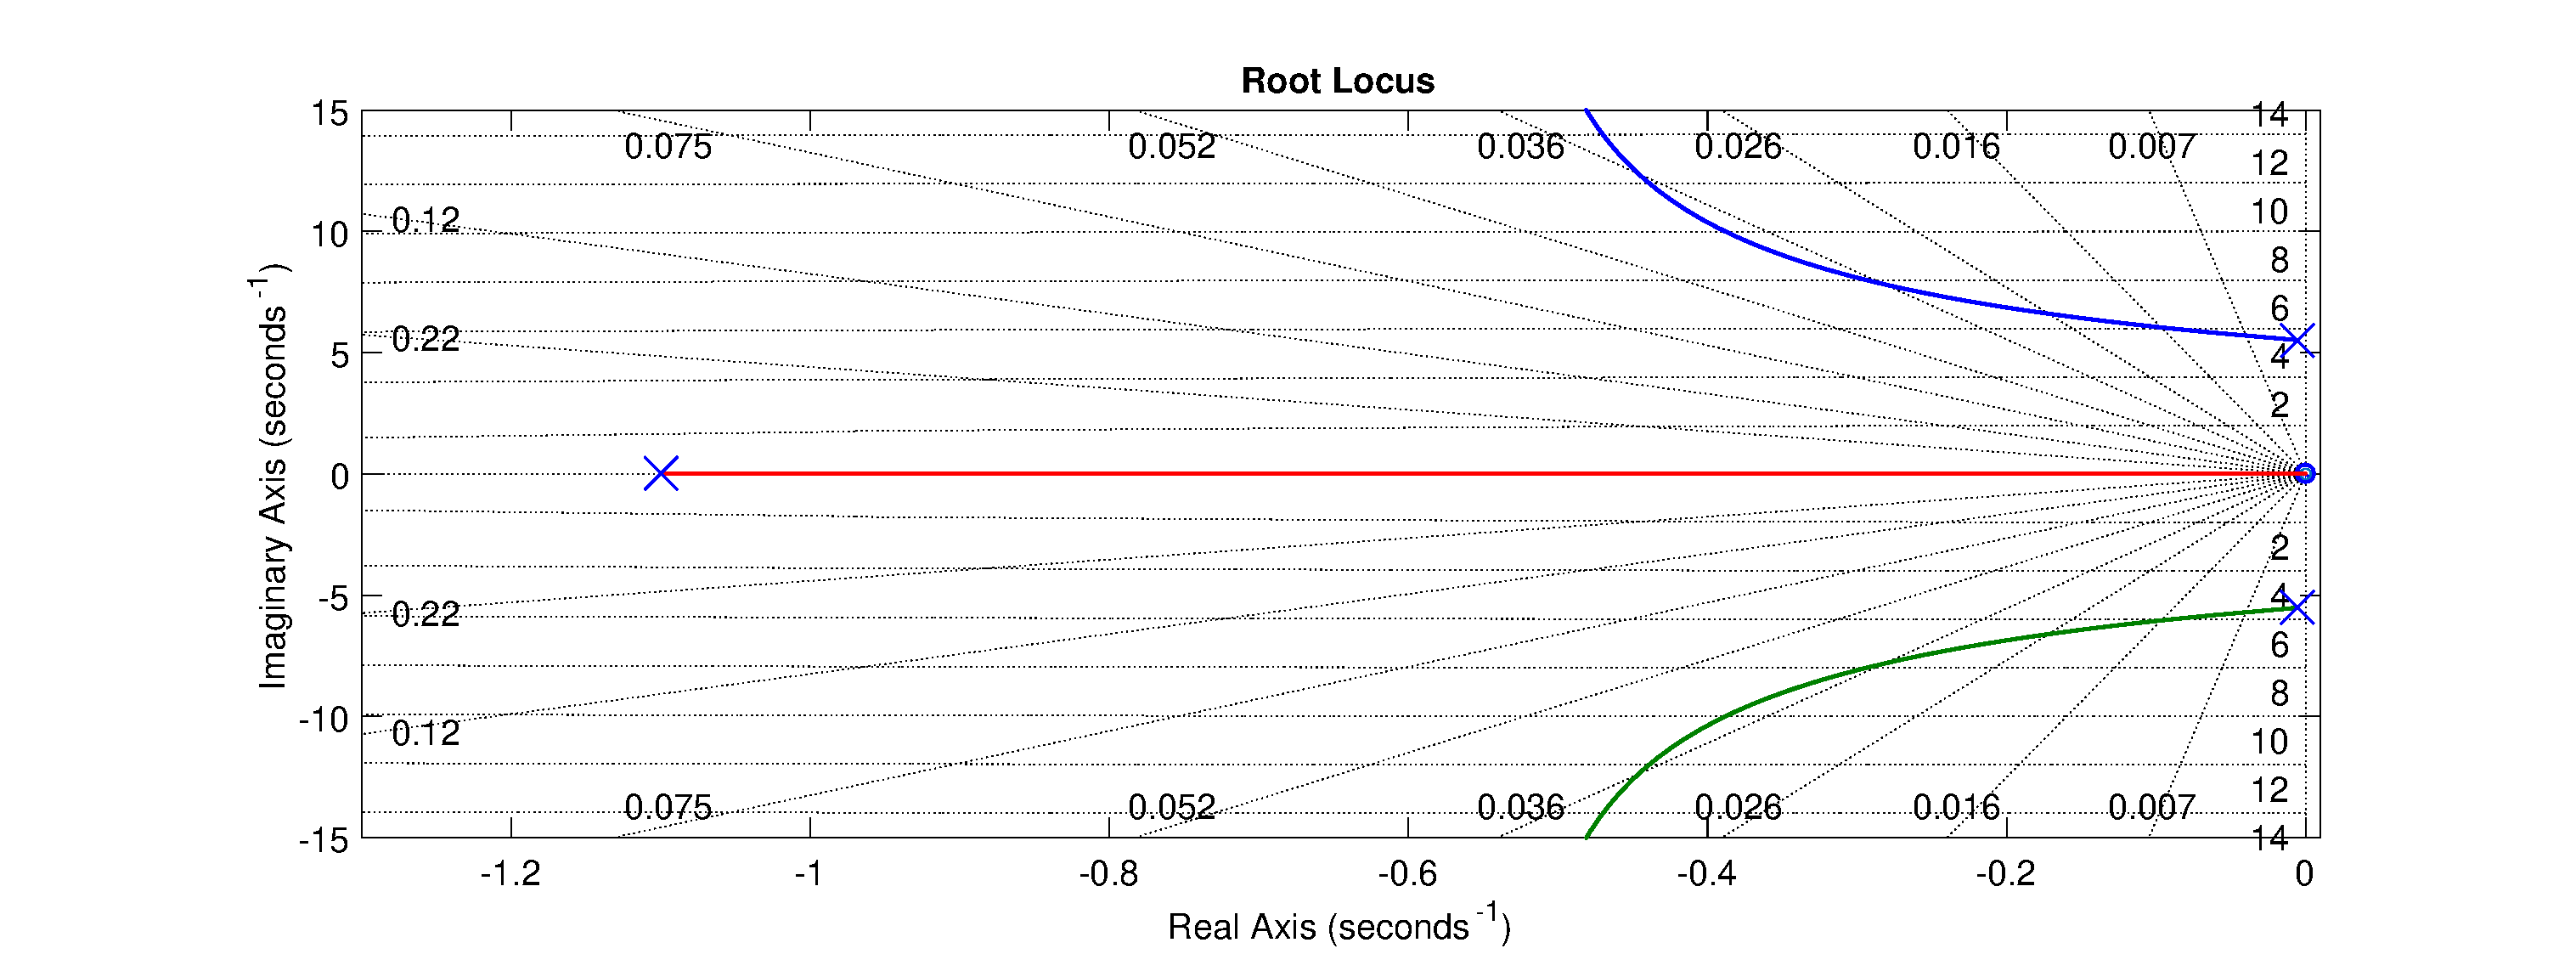
\includegraphics[width=1\textwidth]{billeder/Thomas/AngleConRL11}
\end{figure}
\end{frame}


\begin{frame}{Regulatorer}{Root locus vinkel}
\vspace{1cm}
\begin{figure}[H]
\centering
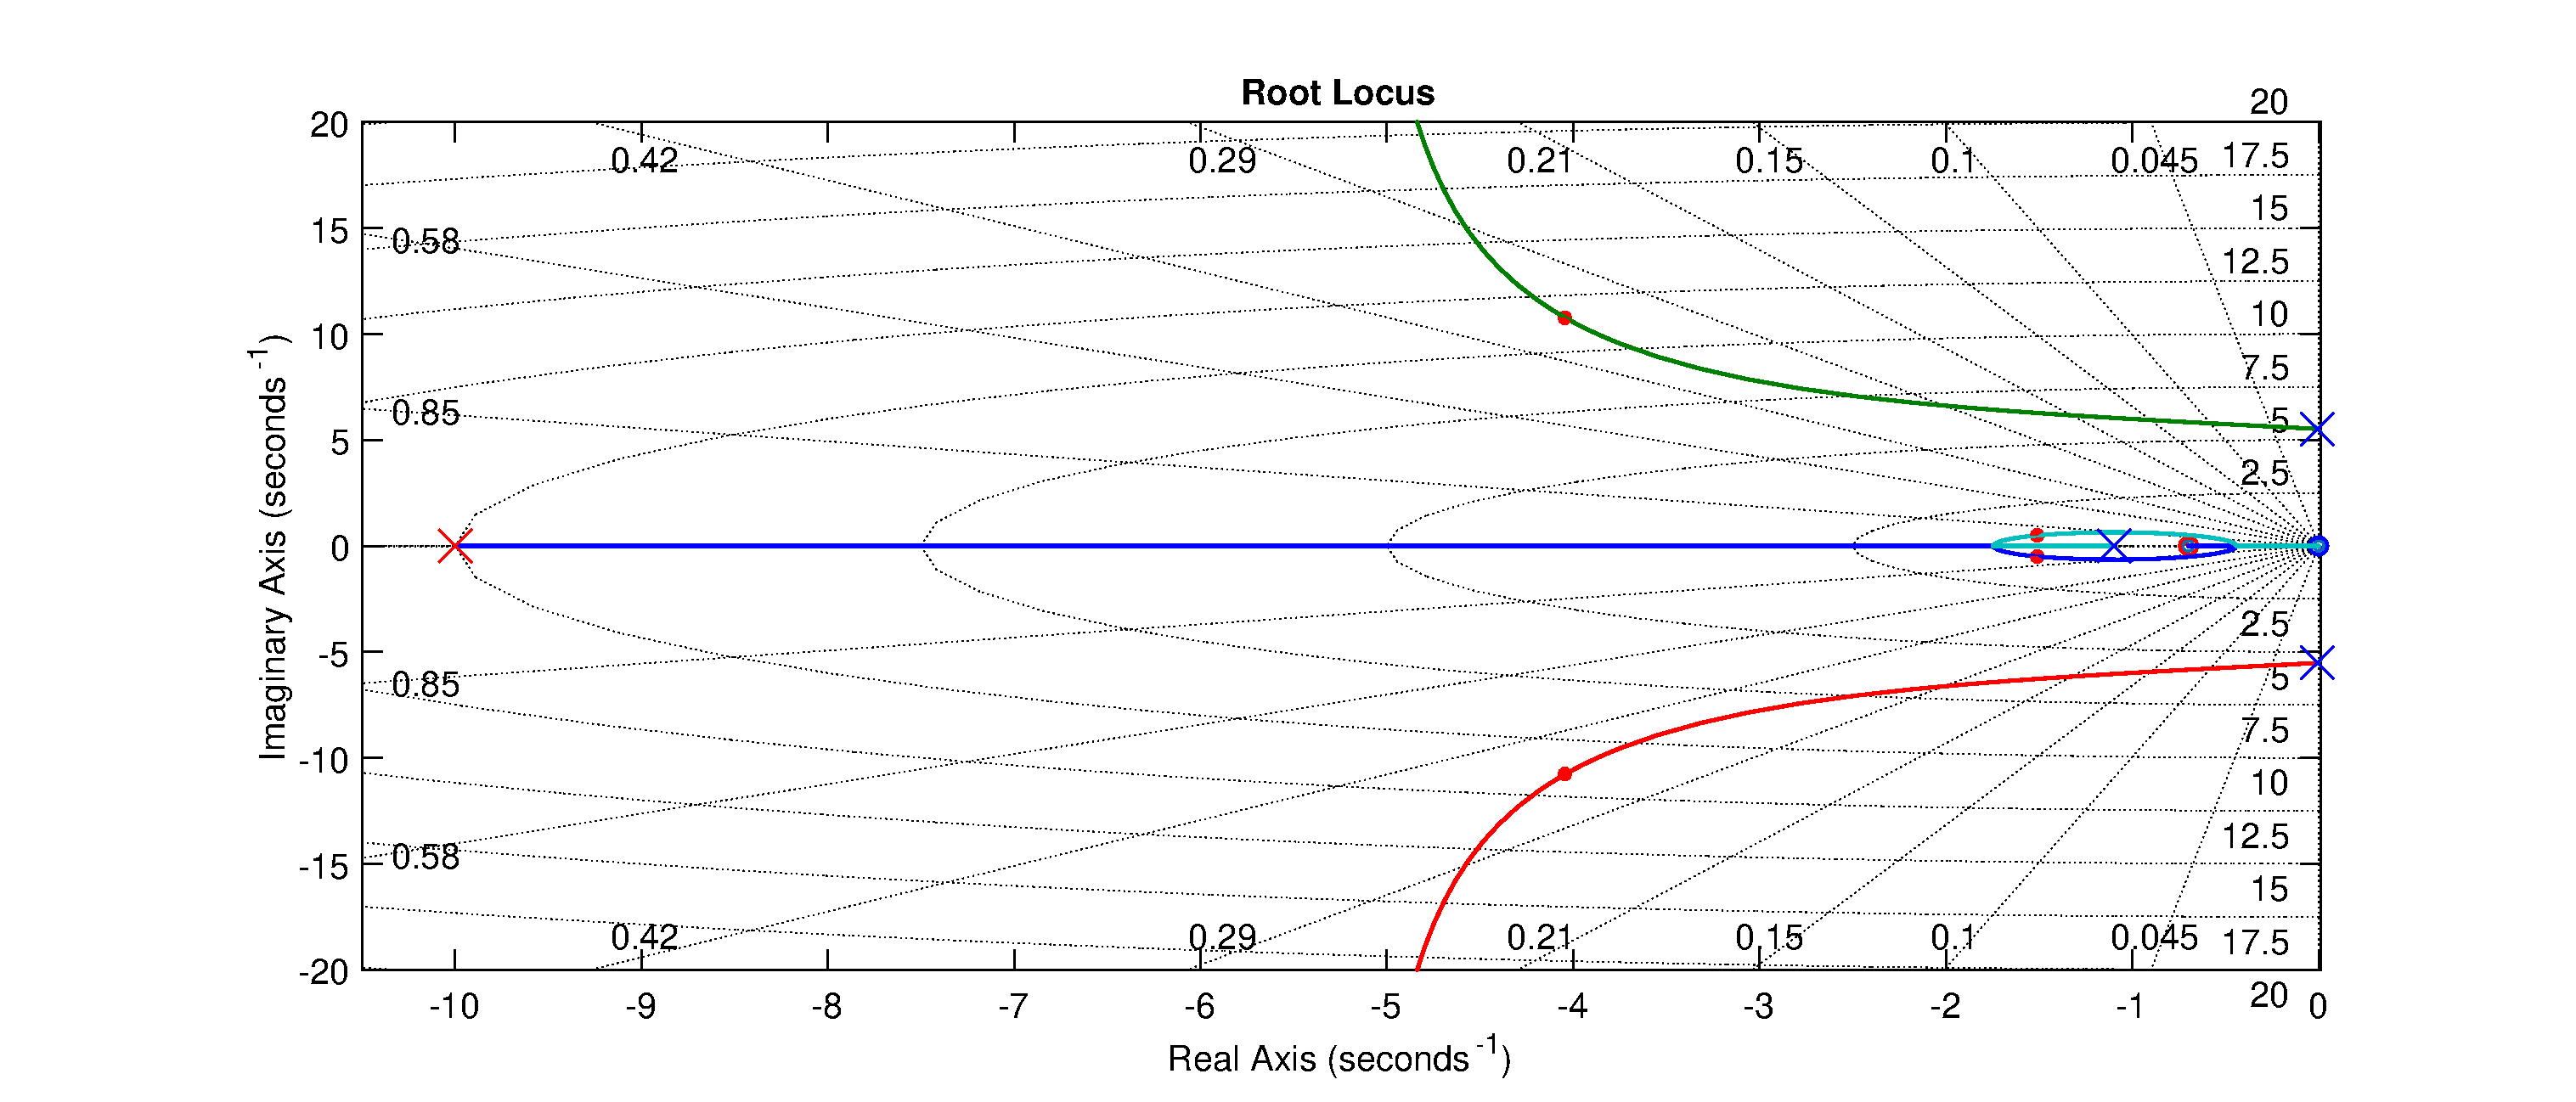
\includegraphics[width=1\textwidth]{Billeder/Thomas/AngleOpenLoop}
\end{figure}
\end{frame}

\begin{frame}{Regulatorer}{Closed loop step respons vinkel}
\begin{figure}[H]
\vspace{1.5cm}
\centering
%\includegraphics[width=0.9\textwidth]{Billeder/Thomas/AngleClosedloopstep}
%\scalebox{0.8} {
% This file was created by matlab2tikz.
%
%The latest updates can be retrieved from
%  http://www.mathworks.com/matlabcentral/fileexchange/22022-matlab2tikz-matlab2tikz
%where you can also make suggestions and rate matlab2tikz.
%
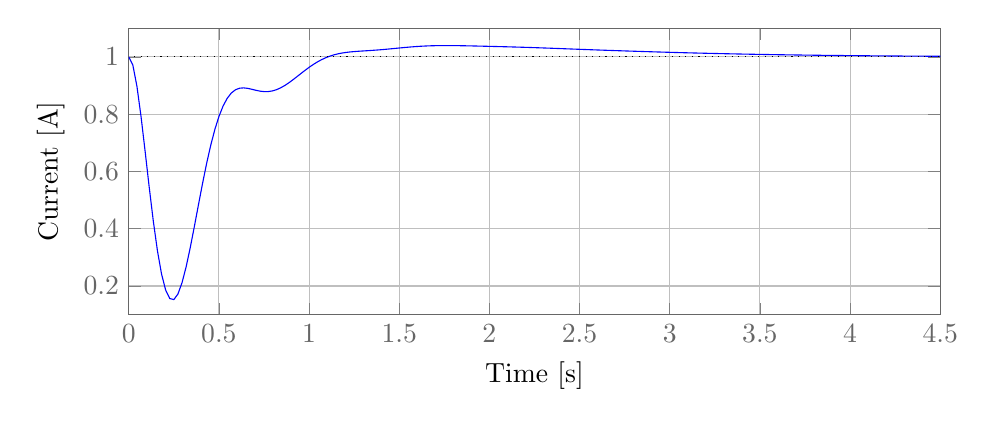
\begin{tikzpicture}

\begin{axis}[%
width=0.85\textwidth,
height=0.3\textwidth,
at={(1.975in,0.746in)},
scale only axis,
separate axis lines,
every outer x axis line/.append style={white!40!black},
every x tick label/.append style={font=\color{white!40!black}},
xmin=0,
xmax=4.5,
xmajorgrids,
xlabel={Time [s]},
every outer y axis line/.append style={white!40!black},
every y tick label/.append style={font=\color{white!40!black}},
ymin=0.1,
ymax=1.1,
ymajorgrids,
ylabel={Current [A]},
axis background/.style={fill=white}
]
\addplot [color=blue,solid,forget plot]
  table[row sep=crcr]{%
0	1\\
0.0227528486535158	0.971859342603638\\
0.0455056973070316	0.897524231115418\\
0.0682585459605474	0.792150043886678\\
0.0910113946140632	0.670163067738347\\
0.113764243267579	0.544486412878134\\
0.136517091921095	0.425989911749438\\
0.159269940574611	0.323160692862605\\
0.182022789228126	0.241977890238838\\
0.204775637881642	0.185964977835278\\
0.227528486535158	0.156386580876281\\
0.250281335188674	0.152553166204965\\
0.27303418384219	0.172196430847109\\
0.295787032495705	0.211880046050608\\
0.318539881149221	0.267414150993223\\
0.341292729802737	0.334247073212653\\
0.364045578456253	0.407813637612809\\
0.386798427109769	0.483825610062481\\
0.409551275763284	0.558495868399752\\
0.4323041244168	0.628693448415354\\
0.455056973070316	0.69203141084787\\
0.477809821723832	0.746893345030093\\
0.500562670377348	0.792407180086614\\
0.523315519030863	0.828376807761253\\
0.546068367684379	0.855182889470085\\
0.568821216337895	0.873664232060762\\
0.591574064991411	0.884990415385541\\
0.614326913644927	0.89053510397904\\
0.637079762298443	0.891757845454882\\
0.659832610951958	0.890100315252366\\
0.682585459605474	0.886901062103816\\
0.70533830825899	0.883330970566316\\
0.728091156912506	0.880349989690254\\
0.750844005566021	0.87868425581915\\
0.773596854219537	0.878821609995853\\
0.796349702873053	0.881022697545281\\
0.819102551526569	0.885344336971374\\
0.841855400180085	0.891671636041704\\
0.864608248833601	0.899755378926245\\
0.887361097487116	0.909251463690159\\
0.910113946140632	0.91975958311996\\
0.932866794794148	0.930858861320235\\
0.955619643447664	0.942138733504533\\
0.978372492101179	0.953223941654054\\
1.0011253407547	0.963793075940382\\
1.02387818940821	0.973590590905626\\
1.04663103806173	0.982432644961956\\
1.06938388671524	0.990207438979097\\
1.09213673536876	0.996870959668754\\
1.11488958402227	1.00243916814705\\
1.13764243267579	1.00697772107355\\
1.16039528132931	1.01059028293757\\
1.18314812998282	1.01340639794986\\
1.20590097863634	1.01556975454151\\
1.22865382728985	1.01722751076157\\
1.25140667594337	1.01852117011482\\
1.27415952459689	1.01957931811851\\
1.2969123732504	1.02051236136967\\
1.31966522190392	1.02140926191499\\
1.34241807055743	1.02233613623442\\
1.36517091921095	1.02333649360878\\
1.38792376786446	1.02443282407827\\
1.41067661651798	1.02562921060417\\
1.4334294651715	1.0269146307687\\
1.45618231382501	1.02826662654221\\
1.47893516247853	1.02965505170559\\
1.50168801113204	1.03104565049479\\
1.52444085978556	1.03240327301125\\
1.54719370843907	1.03369458832426\\
1.56994655709259	1.03489021094625\\
1.59269940574611	1.03596620717336\\
1.61545225439962	1.03690499214155\\
1.63820510305314	1.03769566466607\\
1.66095795170665	1.03833385411714\\
1.68371080036017	1.03882117155764\\
1.70646364901369	1.03916436655656\\
1.7292164976672	1.03937429239917\\
1.75196934632072	1.03946477708488\\
1.77472219497423	1.03945148698639\\
1.79747504362775	1.03935085586951\\
1.82022789228126	1.03917913564089\\
1.84298074093478	1.03895160808656\\
1.8657335895883	1.0386819801841\\
1.88848643824181	1.03838197028746\\
1.91123928689533	1.03806107931539\\
1.93399213554884	1.03772653048864\\
1.95674498420236	1.03738335338537\\
1.97949783285587	1.03703458313001\\
2.00225068150939	1.03668154323504\\
2.02500353016291	1.03632418067177\\
2.04775637881642	1.03596142375786\\
2.07050922746994	1.03559153695995\\
2.09326207612345	1.03521245124878\\
2.11601492477697	1.03482205375438\\
2.13876777343049	1.03441842573545\\
2.161520622084	1.0340000229439\\
2.18427347073752	1.0335657970507\\
2.20702631939103	1.03311526069578\\
2.22977916804455	1.03264850180705\\
2.25253201669806	1.03216615504416\\
2.27528486535158	1.03166933957118\\
2.2980377140051	1.03115957290934\\
2.32079056265861	1.0306386704669\\
2.34354341131213	1.03010863961583\\
2.36629625996564	1.02957157602595\\
2.38904910861916	1.02902956852197\\
2.41180195727268	1.02848461713526\\
2.43455480592619	1.0279385674054\\
2.45730765457971	1.02739306245079\\
2.48006050323322	1.02684951295589\\
2.50281335188674	1.02630908407241\\
2.52556620054025	1.02577269733815\\
2.54831904919377	1.02524104509233\\
2.57107189784729	1.02471461450461\\
2.5938247465008	1.02419371821404\\
2.61657759515432	1.02367852866179\\
2.63933044380783	1.02316911345674\\
2.66208329246135	1.02266546949134\\
2.68483614111486	1.02216755398311\\
2.70758898976838	1.02167531111203\\
2.7303418384219	1.02118869341868\\
2.75309468707541	1.02070767759222\\
2.77584753572893	1.02023227468631\\
2.79860038438244	1.01976253513927\\
2.82135323303596	1.01929854923261\\
2.84410608168948	1.01884044379715\\
2.86685893034299	1.01838837607103\\
2.88961177899651	1.01794252563656\\
2.91236462765002	1.0175030853243\\
2.93511747630354	1.01707025188468\\
2.95787032495705	1.01664421710488\\
2.98062317361057	1.01622515990421\\
3.00337602226409	1.01581323978794\\
3.0261288709176	1.01540859188816\\
3.04888171957112	1.01501132368073\\
3.07163456822463	1.0146215133451\\
3.09438741687815	1.01423920963487\\
3.11714026553167	1.01386443305275\\
3.13989311418518	1.01349717807473\\
3.1626459628387	1.01313741614406\\
3.18539881149221	1.01278509915249\\
3.20815166014573	1.01244016314181\\
3.23090450879924	1.0121025319882\\
3.25365735745276	1.01177212087137\\
3.27641020610628	1.01144883937562\\
3.29916305475979	1.01113259411754\\
3.32191590341331	1.01082329084062\\
3.34466875206682	1.01052083595934\\
3.36742160072034	1.01022513757133\\
3.39017444937385	1.009936105985\\
3.41292729802737	1.00965365383137\\
3.43568014668089	1.00937769584194\\
3.4584329953344	1.00910814838076\\
3.48118584398792	1.00884492881804\\
3.50393869264143	1.00858795482727\\
3.52669154129495	1.00833714367757\\
3.54944438994847	1.00809241158063\\
3.57219723860198	1.00785367313708\\
3.5949500872555	1.00762084091293\\
3.61770293590901	1.00739382516234\\
3.64045578456253	1.00717253370066\\
3.66320863321604	1.00695687192069\\
3.68596148186956	1.00674674293705\\
3.70871433052308	1.00654204783695\\
3.73146717917659	1.00634268601265\\
3.75422002783011	1.0061485555489\\
3.77697287648362	1.00595955363945\\
3.79972572513714	1.00577557700864\\
3.82247857379065	1.00559652231739\\
3.84523142244417	1.00542228653682\\
3.86798427109769	1.00525276727714\\
3.8907371197512	1.00508786306405\\
3.91348996840472	1.00492747355879\\
3.93624281705823	1.00477149972218\\
3.95899566571175	1.00461984392563\\
3.98174851436527	1.00447241001495\\
4.00450136301878	1.00432910333417\\
4.0272542116723	1.00418983071779\\
4.05000706032581	1.00405450045995\\
4.07275990897933	1.0039230222688\\
4.09551275763284	1.00379530721384\\
4.11826560628636	1.00367126767248\\
4.14101845493988	1.00355081728127\\
4.16377130359339	1.00343387089546\\
4.18652415224691	1.00332034455956\\
4.20927700090042	1.00321015548987\\
4.23202984955394	1.00310322206919\\
4.25478269820746	1.00299946385273\\
4.27753554686097	1.00289880158367\\
4.30028839551449	1.00280115721628\\
4.323041244168	1.00270645394423\\
4.34579409282152	1.00261461623172\\
4.36854694147503	1.00252556984512\\
4.39129979012855	1.00243924188299\\
4.41405263878207	1.00235556080296\\
4.43680548743558	1.00227445644383\\
4.4595583360891	1.00219586004231\\
4.48231118474261	1.00211970424361\\
4.50506403339613	1.00204592310599\\
};
\addplot [color=black,dotted,forget plot]
  table[row sep=crcr]{%
-0.45	1\\
0	1\\
1	1\\
4.95000000000005	1\\
};
\end{axis}
\end{tikzpicture}%
%}
\end{figure}
\end{frame}

\begin{frame}{Regulatorer}{Root locus trolley}
\vspace{1cm}
\begin{figure}[H]
\centering
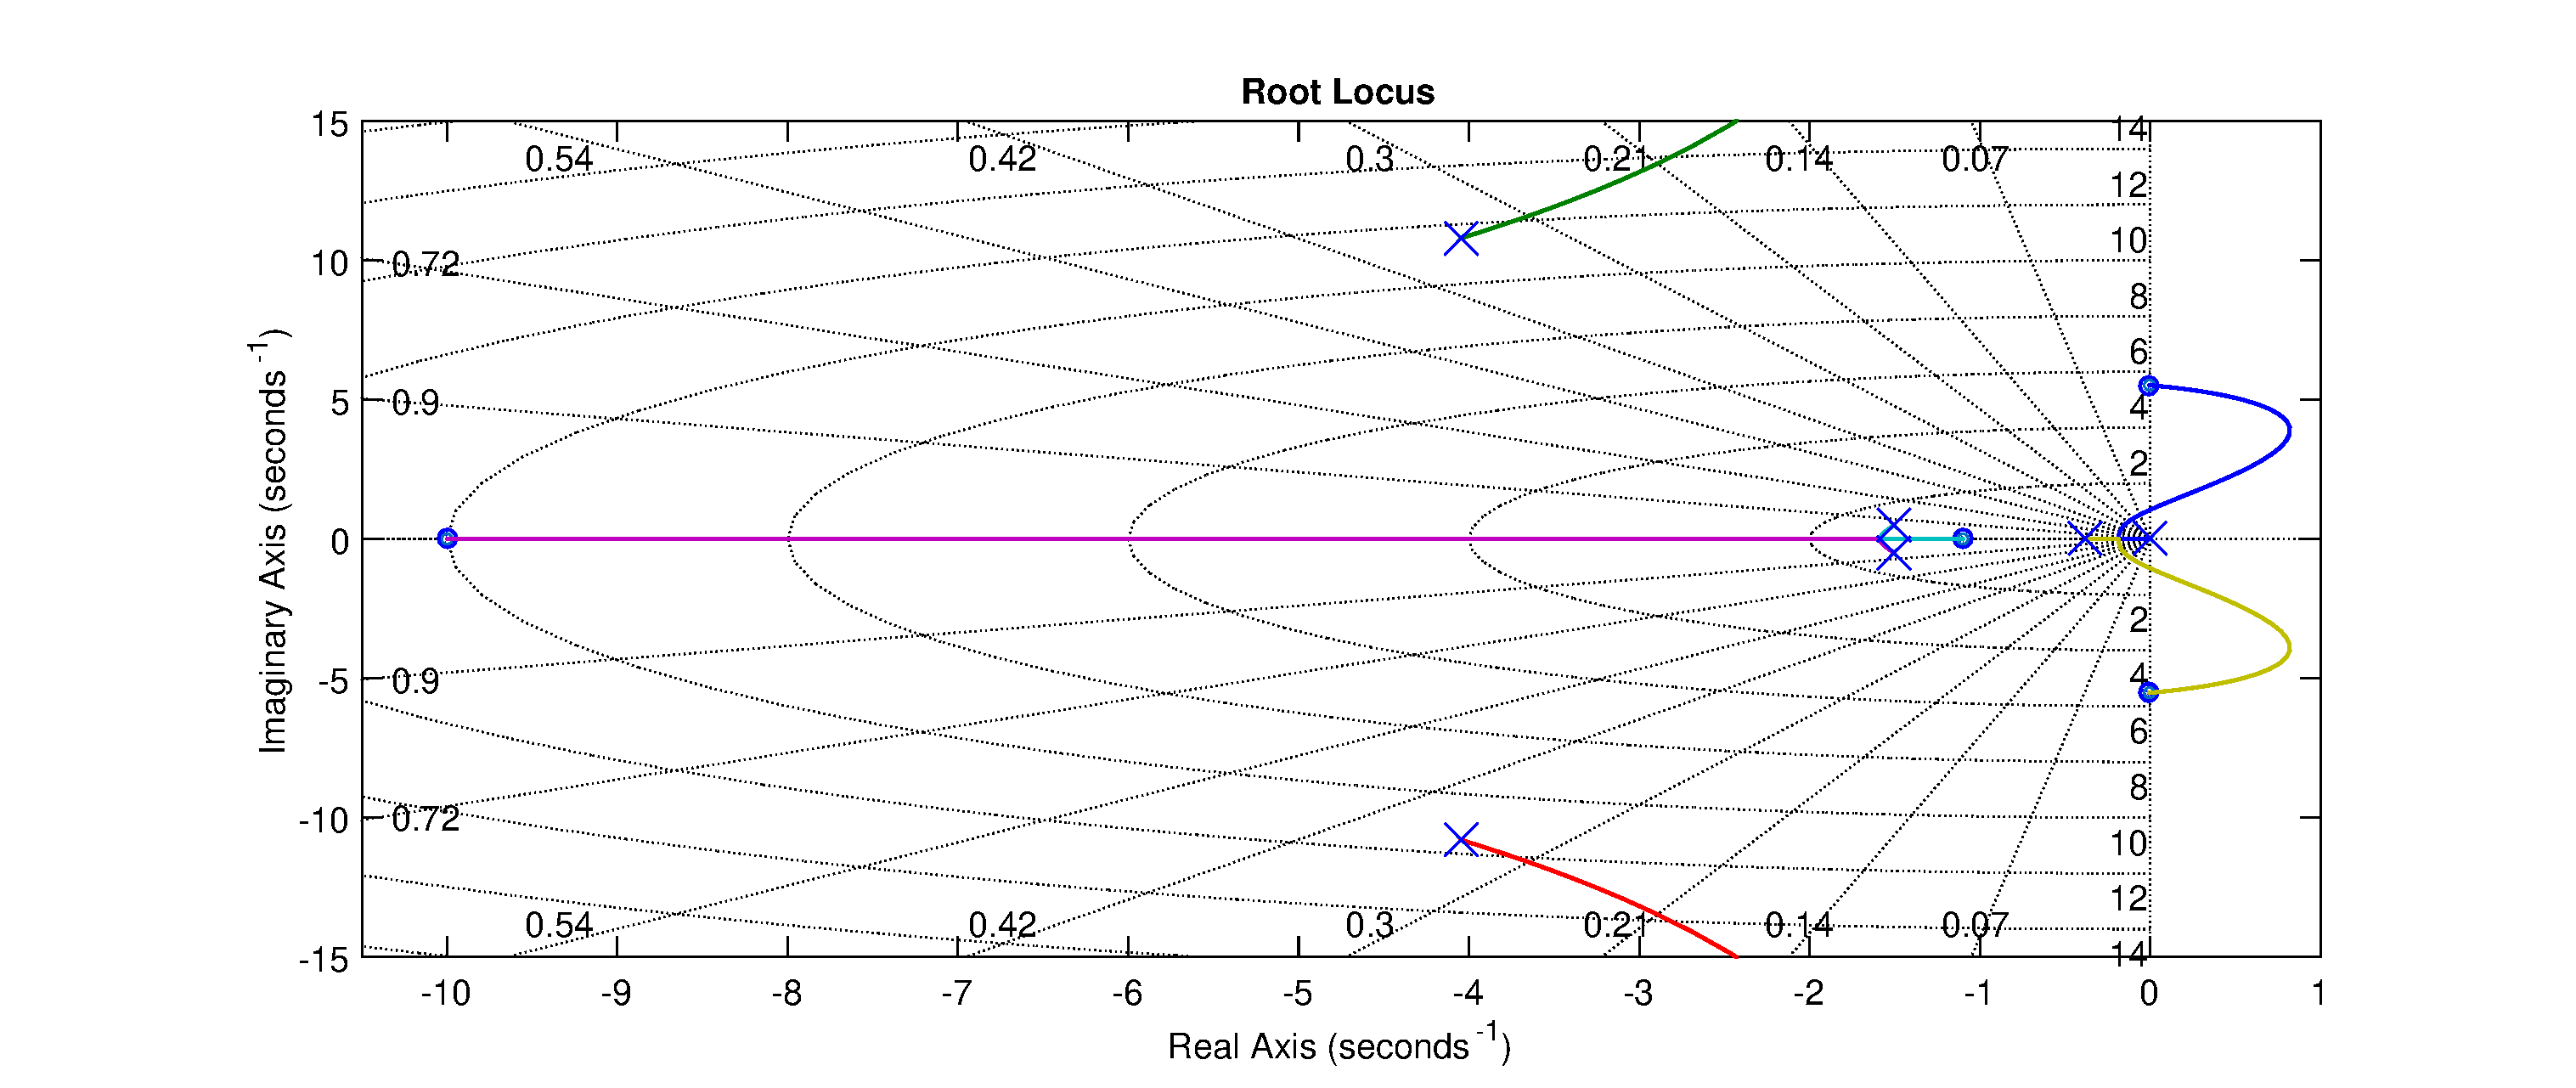
\includegraphics[width=0.9\textwidth]{Billeder/Thomas/Simon}
\end{figure}
\end{frame}

\begin{frame}{Regulatorer}{Root locus trolley}
\vspace{1cm}
\begin{figure}[H]
\centering
\includegraphics[width=0.9\textwidth]{Billeder/Thomas/Trolleyopenloop}
\end{figure}
\end{frame}

\begin{frame}{Regulatorer}{Closed loop step respons trolley}

\begin{figure}[H]
\centering
%\scalebox{0.8} {
% This file was created by matlab2tikz.
%
%The latest updates can be retrieved from
%  http://www.mathworks.com/matlabcentral/fileexchange/22022-matlab2tikz-matlab2tikz
%where you can also make suggestions and rate matlab2tikz.
%
\definecolor{mycolor1}{rgb}{0.00000,0.44700,0.74100}%
%
\begin{tikzpicture}

\begin{axis}[%
width=0.85\textwidth,
height=0.3\textwidth,
at={(2.725in,1.103in)},
scale only axis,
separate axis lines,
every outer x axis line/.append style={white!40!black},
every x tick label/.append style={font=\color{white!40!black}},
xmin=0,
xmax=9,
xmajorgrids,
xlabel={Time [s]},
every outer y axis line/.append style={white!40!black},
every y tick label/.append style={font=\color{white!40!black}},
ymin=0,
ymax=1.1,
ymajorgrids,
ytick={0, 0.2, 0.4, 0.6, 0.8, 1, 1.2},
ylabel={Amplitude},
axis background/.style={fill=white}
]
\addplot [color=mycolor1,solid,forget plot]
  table[row sep=crcr]{%
0	0\\
0.00921034037197597	0.000363485735780711\\
0.0184206807439519	0.00140723474645876\\
0.0276310211159279	0.00306069723582055\\
0.0368413614879039	0.00525334333113738\\
0.0460517018598798	0.00791544763283114\\
0.0552620422318558	0.0109788066726706\\
0.0644723826038318	0.0143773859647359\\
0.0736827229758077	0.0180478943895028\\
0.0828930633477837	0.0219302846556475\\
0.0921034037197597	0.0259681795288045\\
0.101313744091736	0.0301092243950357\\
0.110524084463712	0.0343053675339402\\
0.119734424835688	0.0385130702081035\\
0.128944765207664	0.0426934493290905\\
0.13815510557964	0.0468123560336604\\
0.147365445951615	0.0508403939966198\\
0.156575786323591	0.0547528817190136\\
0.165786126695567	0.0585297633633562\\
0.174996467067543	0.062155472963348\\
0.184206807439519	0.0656187570167473\\
0.193417147811495	0.0689124605801913\\
0.202627488183471	0.0720332820277507\\
0.211837828555447	0.0749815016153273\\
0.221048168927423	0.0777606889154993\\
0.230258509299399	0.0803773940572606\\
0.239468849671375	0.0828408275276593\\
0.248679190043351	0.0851625330731555\\
0.257889530415327	0.0873560579832032\\
0.267099870787303	0.0894366247527076\\
0.276310211159279	0.0914208078091819\\
0.285520551531255	0.0933262186600429\\
0.294730891903231	0.0951712024707945\\
0.303941232275207	0.0969745487308874\\
0.313151572647183	0.0987552183055639\\
0.322361913019159	0.100532088813479\\
0.331572253391135	0.102323719915461\\
0.340782593763111	0.104148139753205\\
0.349992934135087	0.106022653441451\\
0.359203274507063	0.107963674196211\\
0.368413614879039	0.109986577377673\\
0.377623955251015	0.112105577441582\\
0.386834295622991	0.114333627529268\\
0.396044635994967	0.116682341185331\\
0.405254976366943	0.119161935474544\\
0.414465316738919	0.121781194576571\\
0.423675657110894	0.124547452768905\\
0.43288599748287	0.127466595565292\\
0.442096337854846	0.130543077658477\\
0.451306678226822	0.133779956222028\\
0.460517018598798	0.137178938055511\\
0.469727358970774	0.140740439009445\\
0.47893769934275	0.144463654100234\\
0.488148039714726	0.14834663671925\\
0.497358380086702	0.152386385353088\\
0.506568720458678	0.156578936262156\\
0.515779060830654	0.160919460610576\\
0.52498940120263	0.165402364600174\\
0.534199741574606	0.170021391233451\\
0.543410081946582	0.174769722412983\\
0.552620422318558	0.179640080176183\\
0.561830762690534	0.184624825962836\\
0.57104110306251	0.189716056916792\\
0.580251443434486	0.194905698331023\\
0.589461783806462	0.200185591455358\\
0.598672124178438	0.205547575997197\\
0.607882464550414	0.210983566756075\\
0.61709280492239	0.216485623941723\\
0.626303145294366	0.222046016831275\\
0.635513485666342	0.227657280523435\\
0.644723826038318	0.233312265644751\\
0.653934166410294	0.239004180955094\\
0.66314450678227	0.244726628885085\\
0.672354847154246	0.250473634117282\\
0.681565187526222	0.256239665394785\\
0.690775527898198	0.262019650805437\\
0.699985868270174	0.267808986846614\\
0.709196208642149	0.273603541624776\\
0.718406549014125	0.279399652585383\\
0.727616889386101	0.285194119202596\\
0.736827229758077	0.290984191084571\\
0.746037570130053	0.29676755196933\\
0.755247910502029	0.302542300098492\\
0.764458250874005	0.308306925461898\\
0.773668591245981	0.314060284405831\\
0.782878931617957	0.319801572091557\\
0.792089271989933	0.325530293279707\\
0.801299612361909	0.331246231900255\\
0.810509952733885	0.336949419847841\\
0.819720293105861	0.342640105418698\\
0.828930633477837	0.348318721778772\\
0.838140973849813	0.353985855823555\\
0.847351314221789	0.359642217758943\\
0.856561654593765	0.365288611699857\\
0.865771994965741	0.370925907549656\\
0.874982335337717	0.376555014389227\\
0.884192675709693	0.382176855570266\\
0.893403016081669	0.387792345673293\\
0.902613356453645	0.393402369457544\\
0.911823696825621	0.399007762897533\\
0.921034037197597	0.404609296369994\\
0.930244377569573	0.410207660025413\\
0.939454717941549	0.415803451350627\\
0.948665058313525	0.42139716490319\\
0.957875398685501	0.426989184174612\\
0.967085739057477	0.432579775518135\\
0.976296079429452	0.43816908405767\\
0.985506419801428	0.443757131477799\\
0.994716760173404	0.44934381558043\\
1.00392710054538	0.454928911481737\\
1.01313744091736	0.460512074313439\\
1.02234778128933	0.466092843285118\\
1.03155812166131	0.471670646959155\\
1.04076846203328	0.477244809586806\\
1.04997880240526	0.482814558352887\\
1.05918914277724	0.488379031377266\\
1.06839948314921	0.49393728632387\\
1.07760982352119	0.499488309471847\\
1.08682016389316	0.505031025108973\\
1.09603050426514	0.510564305113931\\
1.10524084463712	0.516086978601772\\
1.11445118500909	0.521597841515391\\
1.12366152538107	0.527095666055095\\
1.13287186575304	0.53257920984817\\
1.14208220612502	0.538047224770576\\
1.151292546497	0.543498465343369\\
1.16050288686897	0.548931696637056\\
1.16971322724095	0.554345701627698\\
1.17892356761292	0.559739287958994\\
1.1881339079849	0.565111294074834\\
1.19734424835688	0.570460594696646\\
1.20655458872885	0.575786105629322\\
1.21576492910083	0.581086787888421\\
1.2249752694728	0.586361651149718\\
1.23418560984478	0.591609756529875\\
1.24339595021676	0.596830218714094\\
1.25260629058873	0.602022207452925\\
1.26181663096071	0.607184948456073\\
1.27102697133268	0.612317723715919\\
1.28023731170466	0.617419871297621\\
1.28944765207664	0.622490784636099\\
1.29865799244861	0.627529911382912\\
1.30786833282059	0.632536751848041\\
1.31707867319256	0.637510857082944\\
1.32628901356454	0.642451826651961\\
1.33549935393652	0.647359306139257\\
1.34470969430849	0.652232984438066\\
1.35392003468047	0.657072590868057\\
1.36313037505244	0.661877892165225\\
1.37234071542442	0.666648689386927\\
1.3815510557964	0.671384814772511\\
1.39076139616837	0.676086128597488\\
1.39997173654035	0.680752516056519\\
1.40918207691232	0.685383884207508\\
1.4183924172843	0.689980159006031\\
1.42760275765627	0.694541282456147\\
1.43681309802825	0.699067209900334\\
1.44602343840023	0.703557907468052\\
1.4552337787722	0.708013349699158\\
1.46444411914418	0.712433517355179\\
1.47365445951615	0.716818395428332\\
1.48286479988813	0.721167971355186\\
1.49207514026011	0.72548223343897\\
1.50128548063208	0.729761169481865\\
1.51049582100406	0.734004765626076\\
1.51970616137603	0.73821300540018\\
1.52891650174801	0.742385868965144\\
1.53812684211999	0.746523332552512\\
1.54733718249196	0.750625368085619\\
1.55654752286394	0.754691942973233\\
1.56575786323591	0.75872302006387\\
1.57496820360789	0.762718557747988\\
1.58417854397987	0.766678510194574\\
1.59338888435184	0.770602827708033\\
1.60259922472382	0.774491457190988\\
1.61180956509579	0.778344342698427\\
1.62101990546777	0.78216142606866\\
1.63023024583975	0.785942647616758\\
1.63944058621172	0.789687946876465\\
1.6486509265837	0.793397263377088\\
1.65786126695567	0.797070537442431\\
1.66707160732765	0.80070771099958\\
1.67628194769963	0.804308728386132\\
1.6854922880716	0.807873537145295\\
1.69470262844358	0.811402088799272\\
1.70391296881555	0.81489433959226\\
1.71312330918753	0.818350251195407\\
1.72233364955951	0.821769791367093\\
1.73154398993148	0.825152934562896\\
1.74075433030346	0.828499662490619\\
1.74996467067543	0.831809964606744\\
1.75917501104741	0.835083838551599\\
1.76838535141939	0.83832129052149\\
1.77759569179136	0.841522335576867\\
1.78680603216334	0.844686997886435\\
1.79601637253531	0.847815310907869\\
1.80522671290729	0.850907317506478\\
1.81443705327927	0.853963070013796\\
1.82364739365124	0.856982630228636\\
1.83285773402322	0.859966069363608\\
1.84206807439519	0.862913467940553\\
1.85127841476717	0.86582491563866\\
1.86048875513915	0.868700511099319\\
1.86969909551112	0.871540361691983\\
1.8789094358831	0.874344583245442\\
1.88811977625507	0.877113299749\\
1.89733011662705	0.879846643028079\\
1.90654045699903	0.882544752398735\\
1.915750797371	0.885207774305499\\
1.92496113774298	0.887835861946835\\
1.93417147811495	0.890429174892335\\
1.94338181848693	0.892987878695582\\
1.9525921588589	0.895512144506381\\
1.96180249923088	0.898002148685793\\
1.97101283960286	0.900458072427147\\
1.98022317997483	0.9028801013859\\
1.98943352034681	0.905268425320918\\
1.99864386071878	0.907623237749442\\
2.00785420109076	0.909944735617676\\
2.01706454146274	0.912233118988651\\
2.02627488183471	0.914488590748662\\
2.03548522220669	0.916711356333332\\
2.04469556257866	0.91890162347401\\
2.05390590295064	0.921059601964977\\
2.06311624332262	0.923185503451647\\
2.07232658369459	0.9252795412397\\
2.08153692406657	0.927341930124892\\
2.09074726443854	0.929372886243027\\
2.09995760481052	0.931372626939443\\
2.1091679451825	0.933341370657164\\
2.11837828555447	0.935279336842738\\
2.12758862592645	0.937186745868675\\
2.13679896629842	0.939063818971261\\
2.1460093066704	0.940910778202505\\
2.15521964704238	0.942727846394846\\
2.16442998741435	0.944515247137288\\
2.17364032778633	0.946273204761528\\
2.1828506681583	0.948001944336729\\
2.19206100853028	0.94970169167151\\
2.20127134890226	0.951372673321849\\
2.21048168927423	0.953015116603554\\
2.21969202964621	0.954629249608069\\
2.22890237001818	0.956215301220423\\
2.23811271039016	0.957773501138193\\
2.24732305076214	0.959304079890477\\
2.25653339113411	0.960807268855888\\
2.26574373150609	0.962283300278759\\
2.27495407187806	0.963732407282758\\
2.28416441225004	0.965154823881274\\
2.29337475262202	0.966550784984\\
2.30258509299399	0.967920526399231\\
2.31179543336597	0.969264284831517\\
2.32100577373794	0.970582297874371\\
2.33021611410992	0.971874803997842\\
2.3394264544819	0.973142042530841\\
2.34863679485387	0.97438425363818\\
2.35784713522585	0.975601678292371\\
2.36705747559782	0.976794558240285\\
2.3762678159698	0.977963135964848\\
2.38547815634178	0.97910765464199\\
2.39468849671375	0.980228358093119\\
2.40389883708573	0.98132549073344\\
2.4131091774577	0.982399297516461\\
2.42231951782968	0.983450023875064\\
2.43152985820166	0.984477915659535\\
2.44074019857363	0.985483219072971\\
2.44995053894561	0.986466180604485\\
2.45916087931758	0.987427046960631\\
2.46837121968956	0.988366064995481\\
2.47758156006154	0.989283481639765\\
2.48679190043351	0.990179543829486\\
2.49600224080549	0.991054498434402\\
2.50521258117746	0.991908592186752\\
2.51442292154944	0.99274207161057\\
2.52363326192142	0.993555182951938\\
2.53284360229339	0.994348172110448\\
2.54205394266537	0.99512128457219\\
2.55126428303734	0.995874765344477\\
2.56047462340932	0.996608858892544\\
2.56968496378129	0.997323809078413\\
2.57889530415327	0.998019859102059\\
2.58810564452525	0.998697251445035\\
2.59731598489722	0.999356227816627\\
2.6065263252692	0.999997029102631\\
2.61573666564117	1.00061989531678\\
2.62494700601315	1.00122506555488\\
2.63415734638513	1.00181277795152\\
2.6433676867571	1.00238326963958\\
2.65257802712908	1.00293677671217\\
2.66178836750105	1.00347353418725\\
2.67099870787303	1.00399377597455\\
2.68020904824501	1.00449773484493\\
2.68941938861698	1.004985642402\\
2.69862972898896	1.00545772905576\\
2.70784006936093	1.00591422399833\\
2.71705040973291	1.00635535518152\\
2.72626075010489	1.00678134929605\\
2.73547109047686	1.0071924317525\\
2.74468143084884	1.00758882666353\\
2.75389177122081	1.00797075682756\\
2.76310211159279	1.00833844371352\\
2.77231245196477	1.00869210744668\\
2.78152279233674	1.00903196679537\\
2.79073313270872	1.00935823915851\\
2.79994347308069	1.00967114055375\\
2.80915381345267	1.00997088560625\\
2.81836415382465	1.01025768753789\\
2.82757449419662	1.01053175815681\\
2.8367848345686	1.01079330784732\\
2.84599517494057	1.01104254555997\\
2.85520551531255	1.01127967880178\\
2.86441585568453	1.01150491362661\\
2.8736261960565	1.01171845462551\\
2.88283653642848	1.01192050491717\\
2.89204687680045	1.01211126613834\\
2.90125721717243	1.01229093843413\\
2.91046755754441	1.01245972044845\\
2.91967789791638	1.0126178093142\\
2.92888823828836	1.01276540064359\\
2.93809857866033	1.01290268851832\\
2.94730891903231	1.01302986547979\\
2.95651925940429	1.01314712251924\\
2.96572959977626	1.01325464906804\\
2.97493994014824	1.01335263298787\\
2.98415028052021	1.01344126056106\\
2.99336062089219	1.01352071648108\\
3.00257096126417	1.01359118384302\\
3.01178130163614	1.01365284413441\\
3.02099164200812	1.01370587722612\\
3.03020198238009	1.0137504613636\\
3.03941232275207	1.01378677315826\\
3.04862266312405	1.01381498757935\\
3.05783300349602	1.01383527794599\\
3.067043343868	1.01384781591966\\
3.07625368423997	1.01385277149715\\
3.08546402461195	1.01385031300375\\
3.09467436498392	1.01384060708711\\
3.1038847053559	1.0138238187114\\
3.11309504572788	1.013800111152\\
3.12230538609985	1.01376964599078\\
3.13151572647183	1.01373258311176\\
3.1407260668438	1.0136890806974\\
3.14993640721578	1.01363929522535\\
3.15914674758776	1.0135833814658\\
3.16835708795973	1.01352149247933\\
3.17756742833171	1.01345377961531\\
3.18677776870368	1.01338039251081\\
3.19598810907566	1.01330147909011\\
3.20519844944764	1.01321718556462\\
3.21440878981961	1.01312765643344\\
3.22361913019159	1.0130330344843\\
3.23282947056356	1.01293346079508\\
3.24203981093554	1.01282907473574\\
3.25125015130752	1.01272001397076\\
3.26046049167949	1.01260641446197\\
3.26967083205147	1.01248841047182\\
3.27888117242344	1.01236613456713\\
3.28809151279542	1.01223971762308\\
3.2973018531674	1.01210928882769\\
3.30651219353937	1.01197497568663\\
3.31572253391135	1.0118369040283\\
3.32493287428332	1.01169519800933\\
3.3341432146553	1.01154998012025\\
3.34335355502728	1.01140137119157\\
3.35256389539925	1.01124949040001\\
3.36177423577123	1.01109445527505\\
3.3709845761432	1.01093638170567\\
3.38019491651518	1.01077538394736\\
3.38940525688716	1.01061157462924\\
3.39861559725913	1.0104450647615\\
3.40782593763111	1.01027596374286\\
3.41703627800308	1.01010437936837\\
3.42624661837506	1.00993041783722\\
3.43545695874704	1.0097541837608\\
3.44466729911901	1.00957578017084\\
3.45387763949099	1.00939530852773\\
3.46308797986296	1.00921286872891\\
3.47229832023494	1.00902855911746\\
3.48150866060692	1.00884247649072\\
3.49071900097889	1.00865471610911\\
3.49992934135087	1.00846537170498\\
3.50913968172284	1.00827453549164\\
3.51835002209482	1.0080822981724\\
3.5275603624668	1.00788874894984\\
3.53677070283877	1.00769397553506\\
3.54598104321075	1.00749806415711\\
3.55519138358272	1.00730109957248\\
3.5644017239547	1.00710316507467\\
3.57361206432667	1.00690434250395\\
3.58282240469865	1.00670471225709\\
3.59203274507063	1.00650435329728\\
3.6012430854426	1.00630334316413\\
3.61045342581458	1.00610175798371\\
3.61966376618655	1.00589967247878\\
3.62887410655853	1.00569715997904\\
3.63808444693051	1.00549429243148\\
3.64729478730248	1.00529114041088\\
3.65650512767446	1.00508777313037\\
3.66571546804643	1.00488425845203\\
3.67492580841841	1.0046806628977\\
3.68413614879039	1.00447705165973\\
3.69334648916236	1.00427348861199\\
3.70255682953434	1.00407003632077\\
3.71176716990631	1.00386675605597\\
3.72097751027829	1.00366370780217\\
3.73018785065027	1.00346095026993\\
3.73939819102224	1.00325854090712\\
3.74860853139422	1.00305653591025\\
3.75781887176619	1.002854990236\\
3.76702921213817	1.00265395761268\\
3.77623955251015	1.00245349055188\\
3.78544989288212	1.00225364036007\\
3.7946602332541	1.00205445715031\\
3.80387057362607	1.00185598985403\\
3.81308091399805	1.00165828623277\\
3.82229125437003	1.00146139289006\\
3.831501594742	1.00126535528331\\
3.84071193511398	1.00107021773567\\
3.84992227548595	1.00087602344804\\
3.85913261585793	1.00068281451097\\
3.86834295622991	1.00049063191669\\
3.87755329660188	1.00029951557114\\
3.88676363697386	1.00010950430595\\
3.89597397734583	0.99992063589049\\
3.90518431771781	0.999732947043924\\
3.91439465808979	0.999546473447249\\
3.92360499846176	0.999361249755336\\
3.93281533883374	0.999177309608974\\
3.94202567920571	0.998994685646907\\
3.95123601957769	0.998813409517855\\
3.96044635994967	0.998633511892525\\
3.96965670032164	0.99845502247561\\
3.97886704069362	0.99827797001776\\
3.98807738106559	0.998102382327539\\
3.99728772143757	0.997928286283355\\
4.00649806180955	0.997755707845364\\
4.01570840218152	0.997584672067342\\
4.0249187425535	0.99741520310853\\
4.03412908292547	0.997247324245446\\
4.04333942329745	0.997081057883656\\
4.05254976366943	0.996916425569514\\
4.0617601040414	0.996753448001862\\
4.07097044441338	0.996592145043687\\
4.08018078478535	0.996432535733739\\
4.08939112515733	0.996274638298102\\
4.09860146552931	0.996118470161724\\
4.10781180590128	0.995964047959894\\
4.11702214627326	0.995811387549685\\
4.12623248664523	0.995660504021328\\
4.13544282701721	0.995511411709556\\
4.14465316738919	0.995364124204882\\
4.15386350776116	0.995218654364832\\
4.16307384813314	0.995075014325124\\
4.17228418850511	0.99493321551079\\
4.18149452887709	0.994793268647242\\
4.19070486924906	0.994655183771289\\
4.19991520962104	0.994518970242084\\
4.20912554999302	0.994384636752024\\
4.21833589036499	0.994252191337587\\
4.22754623073697	0.994121641390103\\
4.23675657110894	0.993992993666471\\
4.24596691148092	0.993866254299814\\
4.2551772518529	0.993741428810063\\
4.26438759222487	0.99361852211449\\
4.27359793259685	0.993497538538158\\
4.28280827296882	0.993378481824327\\
4.2920186133408	0.993261355144775\\
4.30122895371278	0.993146161110058\\
4.31043929408475	0.99303290177971\\
4.31964963445673	0.992921578672357\\
4.3288599748287	0.992812192775777\\
4.33807031520068	0.992704744556875\\
4.34728065557266	0.992599233971602\\
4.35649099594463	0.992495660474786\\
4.36570133631661	0.9923940230299\\
4.37491167668858	0.992294320118749\\
4.38412201706056	0.99219654975109\\
4.39333235743254	0.992100709474169\\
4.40254269780451	0.992006796382183\\
4.41175303817649	0.99191480712567\\
4.42096337854846	0.991824737920818\\
4.43017371892044	0.991736584558689\\
4.43938405929242	0.991650342414378\\
4.44859439966439	0.991566006456082\\
4.45780474003637	0.991483571254088\\
4.46701508040834	0.991403030989689\\
4.47622542078032	0.991324379464014\\
4.4854357611523	0.99124761010677\\
4.49464610152427	0.991172715984912\\
4.50385644189625	0.991099689811228\\
4.51306678226822	0.991028523952833\\
4.5222771226402	0.990959210439596\\
4.53148746301218	0.990891740972461\\
4.54069780338415	0.990826106931706\\
4.54990814375613	0.990762299385104\\
4.5591184841281	0.990700309096004\\
4.56832882450008	0.990640126531328\\
4.57753916487206	0.99058174186948\\
4.58674950524403	0.990525145008174\\
4.59595984561601	0.990470325572174\\
4.60517018598798	0.990417272920952\\
4.61438052635996	0.990365976156253\\
4.62359086673194	0.990316424129587\\
4.63280120710391	0.990268605449622\\
4.64201154747589	0.990222508489503\\
4.65122188784786	0.990178121394078\\
4.66043222821984	0.990135432087043\\
4.66964256859182	0.990094428278\\
4.67885290896379	0.990055097469428\\
4.68806324933577	0.990017426963574\\
4.69727358970774	0.989981403869255\\
4.70648393007972	0.989947015108574\\
4.71569427045169	0.989914247423556\\
4.72490461082367	0.989883087382695\\
4.73411495119565	0.98985352138742\\
4.74332529156762	0.989825535678473\\
4.7525356319396	0.98979911634221\\
4.76174597231157	0.989774249316806\\
4.77095631268355	0.989750920398393\\
4.78016665305553	0.989729115247101\\
4.7893769934275	0.989708819393018\\
4.79858733379948	0.989690018242079\\
4.80779767417145	0.989672697081856\\
4.81700801454343	0.989656841087275\\
4.82621835491541	0.989642435326254\\
4.83542869528738	0.989629464765251\\
4.84463903565936	0.989617914274737\\
4.85384937603133	0.989607768634584\\
4.86305971640331	0.989599012539379\\
4.87227005677529	0.989591630603647\\
4.88148039714726	0.989585607367008\\
4.89069073751924	0.989580927299239\\
4.89990107789121	0.989577574805274\\
4.90911141826319	0.989575534230107\\
4.91832175863517	0.989574789863632\\
4.92753209900714	0.989575325945398\\
4.93674243937912	0.989577126669283\\
4.94595277975109	0.989580176188103\\
4.95516312012307	0.989584458618127\\
4.96437346049505	0.989589958043535\\
4.97358380086702	0.989596658520783\\
4.982794141239	0.989604544082901\\
4.99200448161097	0.989613598743718\\
5.00121482198295	0.989623806502009\\
5.01042516235493	0.989635151345564\\
5.0196355027269	0.989647617255192\\
5.02884584309888	0.989661188208648\\
5.03805618347085	0.989675848184485\\
5.04726652384283	0.989691581165834\\
5.05647686421481	0.98970837114412\\
5.06568720458678	0.989726202122699\\
5.07489754495876	0.989745058120423\\
5.08410788533073	0.989764923175144\\
5.09331822570271	0.989785781347138\\
5.10252856607469	0.989807616722473\\
5.11173890644666	0.989830413416288\\
5.12094924681864	0.989854155576032\\
5.13015958719061	0.989878827384605\\
5.13936992756259	0.98990441306346\\
5.14858026793457	0.989930896875618\\
5.15779060830654	0.989958263128629\\
5.16700094867852	0.989986496177465\\
5.17621128905049	0.990015580427343\\
5.18542162942247	0.990045500336496\\
5.19463196979445	0.990076240418866\\
5.20384231016642	0.990107785246747\\
5.2130526505384	0.990140119453357\\
5.22226299091037	0.990173227735351\\
5.23147333128235	0.990207094855279\\
5.24068367165432	0.99024170564397\\
5.2498940120263	0.990277045002869\\
5.25910435239828	0.99031309790631\\
5.26831469277025	0.990349849403727\\
5.27752503314223	0.990387284621812\\
5.2867353735142	0.990425388766616\\
5.29594571388618	0.990464147125585\\
5.30515605425816	0.99050354506955\\
5.31436639463013	0.990543568054653\\
5.32357673500211	0.990584201624226\\
5.33278707537408	0.990625431410608\\
5.34199741574606	0.990667243136911\\
5.35120775611804	0.990709622618735\\
5.36041809649001	0.990752555765829\\
5.36962843686199	0.990796028583697\\
5.37883877723396	0.990840027175154\\
5.38804911760594	0.990884537741836\\
5.39725945797792	0.990929546585657\\
5.40646979834989	0.990975040110208\\
5.41568013872187	0.991021004822121\\
5.42489047909384	0.991067427332377\\
5.43410081946582	0.991114294357566\\
5.4433111598378	0.991161592721101\\
5.45252150020977	0.991209309354386\\
5.46173184058175	0.991257431297938\\
5.47094218095372	0.991305945702463\\
5.4801525213257	0.991354839829887\\
5.48936286169768	0.991404101054343\\
5.49857320206965	0.991453716863117\\
5.50778354244163	0.991503674857546\\
5.5169938828136	0.991553962753876\\
5.52620422318558	0.991604568384081\\
5.53541456355756	0.991655479696637\\
5.54462490392953	0.991706684757257\\
5.55383524430151	0.991758171749585\\
5.56304558467348	0.991809928975853\\
5.57225592504546	0.991861944857494\\
5.58146626541744	0.991914207935723\\
5.59067660578941	0.991966706872078\\
5.59988694616139	0.992019430448919\\
5.60909728653336	0.9920723675699\\
5.61830762690534	0.992125507260393\\
5.62751796727732	0.992178838667891\\
5.63672830764929	0.992232351062363\\
5.64593864802127	0.99228603383658\\
5.65514898839324	0.99233987650641\\
5.66435932876522	0.992393868711075\\
5.6735696691372	0.992448000213378\\
5.68278000950917	0.992502260899899\\
5.69199034988115	0.992556640781152\\
5.70120069025312	0.992611129991726\\
5.7104110306251	0.992665718790376\\
5.71962137099707	0.992720397560102\\
5.72883171136905	0.992775156808188\\
5.73804205174103	0.992829987166216\\
5.747252392113	0.992884879390047\\
5.75646273248498	0.992939824359786\\
5.76567307285695	0.992994813079701\\
5.77488341322893	0.993049836678136\\
5.78409375360091	0.993104886407379\\
5.79330409397288	0.99315995364352\\
5.80251443434486	0.993215029886271\\
5.81172477471683	0.993270106758771\\
5.82093511508881	0.993325176007359\\
5.83014545546079	0.993380229501328\\
5.83935579583276	0.993435259232655\\
5.84856613620474	0.99349025731571\\
5.85777647657671	0.993545215986934\\
5.86698681694869	0.993600127604509\\
5.87619715732067	0.993654984647992\\
5.88540749769264	0.993709779717942\\
5.89461783806462	0.993764505535516\\
5.90382817843659	0.99381915494205\\
5.91303851880857	0.993873720898619\\
5.92224885918055	0.993928196485579\\
5.93145919955252	0.99398257490209\\
5.9406695399245	0.994036849465619\\
5.94987988029647	0.994091013611431\\
5.95909022066845	0.994145060892054\\
5.96830056104043	0.994198984976734\\
5.9775109014124	0.994252779650873\\
5.98672124178438	0.994306438815446\\
5.99593158215635	0.994359956486409\\
6.00514192252833	0.994413326794088\\
6.01435226290031	0.994466543982552\\
6.02356260327228	0.994519602408977\\
6.03277294364426	0.994572496542991\\
6.04198328401623	0.994625220966007\\
6.05119362438821	0.994677770370544\\
6.06040396476019	0.994730139559535\\
6.06961430513216	0.994782323445618\\
6.07882464550414	0.994834317050424\\
6.08803498587611	0.994886115503848\\
6.09724532624809	0.994937714043305\\
6.10645566662007	0.994989108012983\\
6.11566600699204	0.995040292863081\\
6.12487634736402	0.995091264149039\\
6.13408668773599	0.995142017530752\\
6.14329702810797	0.995192548771787\\
6.15250736847995	0.995242853738577\\
6.16171770885192	0.995292928399616\\
6.1709280492239	0.99534276882464\\
6.18013838959587	0.995392371183804\\
6.18934872996785	0.995441731746851\\
6.19855907033983	0.995490846882266\\
6.2077694107118	0.995539713056437\\
6.21697975108378	0.995588326832793\\
6.22619009145575	0.99563668487095\\
6.23540043182773	0.99568478392584\\
6.24461077219971	0.995732620846843\\
6.25382111257168	0.995780192576904\\
6.26303145294366	0.995827496151654\\
6.27224179331563	0.995874528698518\\
6.28145213368761	0.995921287435828\\
6.29066247405959	0.995967769671917\\
6.29987281443156	0.996013972804227\\
6.30908315480354	0.996059894318394\\
6.31829349517551	0.996105531787349\\
6.32750383554749	0.996150882870398\\
6.33671417591947	0.99619594531231\\
6.34592451629144	0.996240716942398\\
6.35513485666342	0.9962851956736\\
6.36434519703539	0.996329379501553\\
6.37355553740737	0.996373266503672\\
6.38276587777935	0.996416854838219\\
6.39197621815132	0.996460142743377\\
6.4011865585233	0.996503128536319\\
6.41039689889527	0.99654581061228\\
6.41960723926725	0.996588187443619\\
6.42881757963923	0.996630257578894\\
6.4380279200112	0.996672019641924\\
6.44723826038318	0.996713472330858\\
6.45644860075515	0.99675461441724\\
6.46565894112713	0.996795444745078\\
6.4748692814991	0.996835962229912\\
6.48407962187108	0.996876165857879\\
6.49328996224306	0.996916054684781\\
6.50250030261503	0.996955627835161\\
6.51171064298701	0.996994884501367\\
6.52092098335898	0.997033823942628\\
6.53013132373096	0.997072445484126\\
6.53934166410294	0.997110748516072\\
6.54855200447491	0.997148732492783\\
6.55776234484689	0.997186396931761\\
6.56697268521886	0.997223741412777\\
6.57618302559084	0.997260765576949\\
6.58539336596282	0.997297469125835\\
6.59460370633479	0.997333851820517\\
6.60381404670677	0.997369913480697\\
6.61302438707874	0.997405653983788\\
6.62223472745072	0.997441073264014\\
6.6314450678227	0.997476171311509\\
6.64065540819467	0.997510948171428\\
6.64986574856665	0.997545403943046\\
6.65907608893862	0.997579538778877\\
6.6682864293106	0.997613352883787\\
6.67749676968258	0.99764684651411\\
6.68670711005455	0.997680019976781\\
6.69591745042653	0.997712873628454\\
6.7051277907985	0.997745407874637\\
6.71433813117048	0.997777623168834\\
6.72354847154246	0.997809520011677\\
6.73275881191443	0.997841098950078\\
6.74196915228641	0.997872360576377\\
6.75117949265838	0.997903305527498\\
6.76038983303036	0.997933934484106\\
6.76960017340234	0.997964248169778\\
6.77881051377431	0.997994247350168\\
6.78802085414629	0.998023932832182\\
6.79723119451826	0.998053305463165\\
6.80644153489024	0.998082366130079\\
6.81565187526222	0.9981111157587\\
6.82486221563419	0.998139555312814\\
6.83407255600617	0.998167685793418\\
6.84328289637814	0.998195508237929\\
6.85249323675012	0.998223023719399\\
6.8617035771221	0.998250233345734\\
6.87091391749407	0.998277138258921\\
6.88012425786605	0.998303739634257\\
6.88933459823802	0.998330038679592\\
6.89854493861	0.998356036634566\\
6.90775527898198	0.998381734769865\\
6.91696561935395	0.998407134386475\\
6.92617595972593	0.998432236814942\\
6.9353863000979	0.998457043414646\\
6.94459664046988	0.99848155557307\\
6.95380698084186	0.998505774705089\\
6.96301732121383	0.998529702252249\\
6.97222766158581	0.998553339682068\\
6.98143800195778	0.998576688487336\\
6.99064834232976	0.998599750185419\\
6.99985868270173	0.998622526317576\\
7.00906902307371	0.998645018448281\\
7.01827936344569	0.998667228164543\\
7.02748970381766	0.998689157075252\\
7.03670004418964	0.998710806810506\\
7.04591038456161	0.99873217902097\\
7.05512072493359	0.998753275377224\\
7.06433106530557	0.998774097569124\\
7.07354140567754	0.998794647305171\\
7.08275174604952	0.998814926311886\\
7.09196208642149	0.99883493633319\\
7.10117242679347	0.998854679129795\\
7.11038276716545	0.998874156478592\\
7.11959310753742	0.998893370172061\\
7.1288034479094	0.998912322017676\\
7.13801378828137	0.998931013837319\\
7.14722412865335	0.998949447466707\\
7.15643446902533	0.998967624754815\\
7.1656448093973	0.998985547563318\\
7.17485514976928	0.999003217766032\\
7.18406549014125	0.999020637248363\\
7.19327583051323	0.999037807906764\\
7.20248617088521	0.999054731648199\\
7.21169651125718	0.999071410389617\\
7.22090685162916	0.999087846057423\\
7.23011719200113	0.999104040586968\\
7.23932753237311	0.999119995922035\\
7.24853787274509	0.999135714014342\\
7.25774821311706	0.999151196823046\\
7.26695855348904	0.999166446314249\\
7.27616889386101	0.999181464460526\\
7.28537923423299	0.999196253240439\\
7.29458957460497	0.999210814638081\\
7.30379991497694	0.999225150642603\\
7.31301025534892	0.99923926324777\\
7.32222059572089	0.999253154451503\\
7.33143093609287	0.999266826255448\\
7.34064127646485	0.999280280664534\\
7.34985161683682	0.999293519686548\\
7.3590619572088	0.999306545331712\\
7.36827229758077	0.999319359612272\\
7.37748263795275	0.999331964542087\\
7.38669297832473	0.999344362136227\\
7.3959033186967	0.999356554410581\\
7.40511365906868	0.999368543381464\\
7.41432399944065	0.999380331065238\\
7.42353433981263	0.999391919477938\\
7.43274468018461	0.999403310634896\\
7.44195502055658	0.999414506550386\\
7.45116536092856	0.999425509237262\\
7.46037570130053	0.99943632070661\\
7.46958604167251	0.999446942967401\\
7.47879638204448	0.999457378026158\\
7.48800672241646	0.99946762788662\\
7.49721706278844	0.999477694549418\\
7.50642740316041	0.999487580011755\\
7.51563774353239	0.999497286267094\\
7.52484808390436	0.99950681530485\\
7.53405842427634	0.999516169110085\\
7.54326876464832	0.999525349663219\\
7.55247910502029	0.999534358939737\\
7.56168944539227	0.999543198909903\\
7.57089978576424	0.999551871538487\\
7.58011012613622	0.99956037878449\\
7.5893204665082	0.999568722600875\\
7.59853080688017	0.999576904934315\\
7.60774114725215	0.999584927724928\\
7.61695148762412	0.999592792906034\\
7.6261618279961	0.999600502403908\\
7.63537216836808	0.999608058137545\\
7.64458250874005	0.999615462018422\\
7.65379284911203	0.999622715950276\\
7.663003189484	0.999629821828879\\
7.67221352985598	0.99963678154182\\
7.68142387022796	0.999643596968297\\
7.69063421059993	0.99965026997891\\
7.69984455097191	0.999656802435457\\
7.70905489134388	0.999663196190742\\
7.71826523171586	0.999669453088381\\
7.72747557208784	0.999675574962618\\
7.73668591245981	0.999681563638146\\
7.74589625283179	0.999687420929927\\
7.75510659320376	0.999693148643024\\
7.76431693357574	0.999698748572436\\
7.77352727394772	0.999704222502932\\
7.78273761431969	0.9997095722089\\
7.79194795469167	0.999714799454192\\
7.80115829506364	0.99971990599198\\
7.81036863543562	0.999724893564608\\
7.8195789758076	0.99972976390346\\
7.82878931617957	0.999734518728822\\
7.83799965655155	0.999739159749757\\
7.84720999692352	0.999743688663976\\
7.8564203372955	0.999748107157724\\
7.86563067766748	0.999752416905656\\
7.87484101803945	0.999756619570731\\
7.88405135841143	0.999760716804106\\
7.8932616987834	0.999764710245025\\
7.90247203915538	0.999768601520729\\
7.91168237952736	0.999772392246354\\
7.92089271989933	0.999776084024843\\
7.93010306027131	0.999779678446859\\
7.93931340064328	0.999783177090699\\
7.94852374101526	0.999786581522218\\
7.95773408138724	0.999789893294752\\
7.96694442175921	0.999793113949045\\
7.97615476213119	0.999796245013182\\
7.98536510250316	0.999799288002526\\
7.99457544287514	0.999802244419652\\
8.00378578324712	0.999805115754296\\
8.01299612361909	0.999807903483296\\
8.02220646399107	0.999810609070546\\
8.03141680436304	0.999813233966945\\
8.04062714473502	0.999815779610356\\
8.04983748510699	0.999818247425563\\
8.05904782547897	0.999820638824239\\
8.06825816585095	0.999822955204906\\
8.07746850622292	0.999825197952908\\
8.0866788465949	0.999827368440382\\
8.09588918696688	0.999829468026236\\
8.10509952733885	0.999831498056124\\
8.11430986771083	0.999833459862429\\
8.1235202080828	0.999835354764248\\
8.13273054845478	0.999837184067377\\
8.14194088882675	0.999838949064306\\
8.15115122919873	0.999840651034205\\
8.16036156957071	0.999842291242927\\
8.16957190994268	0.999843870942999\\
8.17878225031466	0.999845391373629\\
8.18799259068664	0.999846853760706\\
8.19720293105861	0.999848259316807\\
8.20641327143059	0.999849609241207\\
8.21562361180256	0.999850904719886\\
8.22483395217454	0.99985214692555\\
8.23404429254651	0.999853337017637\\
8.24325463291849	0.999854476142344\\
8.25246497329047	0.999855565432642\\
8.26167531366244	0.999856606008302\\
8.27088565403442	0.999857598975916\\
8.28009599440639	0.999858545428928\\
8.28930633477837	0.999859446447662\\
8.29851667515035	0.999860303099352\\
8.30772701552232	0.999861116438177\\
8.3169373558943	0.999861887505294\\
8.32614769626627	0.999862617328877\\
8.33535803663825	0.999863306924157\\
8.34456837701023	0.99986395729346\\
8.3537787173822	0.999864569426252\\
8.36298905775418	0.999865144299181\\
8.37219939812615	0.999865682876129\\
8.38140973849813	0.999866186108252\\
8.39062007887011	0.999866654934038\\
8.39983041924208	0.99986709027935\\
8.40904075961406	0.999867493057486\\
8.41825109998603	0.999867864169228\\
8.42746144035801	0.999868204502903\\
8.43667178072999	0.999868514934434\\
8.44588212110196	0.999868796327406\\
8.45509246147394	0.999869049533121\\
8.46430280184591	0.999869275390661\\
8.47351314221789	0.999869474726952\\
8.48272348258987	0.999869648356826\\
8.49193382296184	0.999869797083089\\
8.50114416333382	0.999869921696586\\
8.51035450370579	0.999870022976269\\
8.51956484407777	0.999870101689267\\
8.52877518444975	0.999870158590953\\
8.53798552482172	0.999870194425022\\
8.5471958651937	0.999870209923553\\
8.55640620556567	0.999870205807093\\
8.56561654593765	0.999870182784722\\
8.57482688630962	0.999870141554137\\
8.5840372266816	0.999870082801719\\
8.59324756705358	0.999870007202617\\
8.60245790742555	0.999869915420822\\
8.61166824779753	0.999869808109248\\
8.62087858816951	0.99986968590981\\
8.63008892854148	0.999869549453505\\
8.63929926891346	0.99986939936049\\
8.64850960928543	0.999869236240171\\
8.65771994965741	0.999869060691276\\
8.66693029002938	0.999868873301945\\
8.67614063040136	0.99986867464981\\
8.68535097077334	0.999868465302082\\
8.69456131114531	0.999868245815633\\
8.70377165151729	0.999868016737082\\
8.71298199188927	0.999867778602882\\
8.72219233226124	0.999867531939406\\
8.73140267263322	0.999867277263031\\
8.74061301300519	0.999867015080231\\
8.74982335337717	0.999866745887658\\
8.75903369374914	0.999866470172236\\
8.76824403412112	0.999866188411243\\
8.7774543744931	0.999865901072407\\
8.78666471486507	0.999865608613988\\
8.79587505523705	0.999865311484871\\
8.80508539560902	0.999865010124657\\
8.814295735981	0.999864704963749\\
8.82350607635298	0.999864396423443\\
8.83271641672495	0.999864084916021\\
8.84192675709693	0.999863770844839\\
8.8511370974689	0.999863454604415\\
8.86034743784088	0.999863136580527\\
8.86955777821286	0.999862817150295\\
8.87876811858483	0.99986249668228\\
8.88797845895681	0.999862175536568\\
8.89718879932878	0.999861854064866\\
8.90639913970076	0.999861532610591\\
8.91560948007274	0.99986121150896\\
8.92481982044471	0.999860891087083\\
8.93403016081669	0.999860571664054\\
8.94324050118866	0.999860253551039\\
8.95245084156064	0.999859937051371\\
8.96166118193262	0.999859622460639\\
8.97087152230459	0.999859310066777\\
8.98008186267657	0.999859000150158\\
8.98929220304854	0.999858692983681\\
8.99850254342052	0.999858388832866\\
9.00771288379249	0.999858087955939\\
};
\end{axis}
\end{tikzpicture}%
%}
%\includegraphics[width=1.1\textwidth]{Billeder/Thomas/cl_x_step}
\end{figure}


\vspace{0.2cm}
\begin{description}
    \item[\textbf{(E)}] : x-akse settling time, $t_s \leq 17,45 s$
    \item[\textbf{(F)}] : x-akse steady-state-error, $e_{ss} = 0,0\%$ 
    \item[\textbf{(G)}] : x-akse overshoot, $M_p \leq 6,4\%$
\end{description}
\vspace{0.6cm}

\end{frame}

\begin{frame}{Regulatorer}{Simulering af closed loop med statisk friktion kompensering}
\vspace{1.5cm}
\begin{figure}[H]
\centering
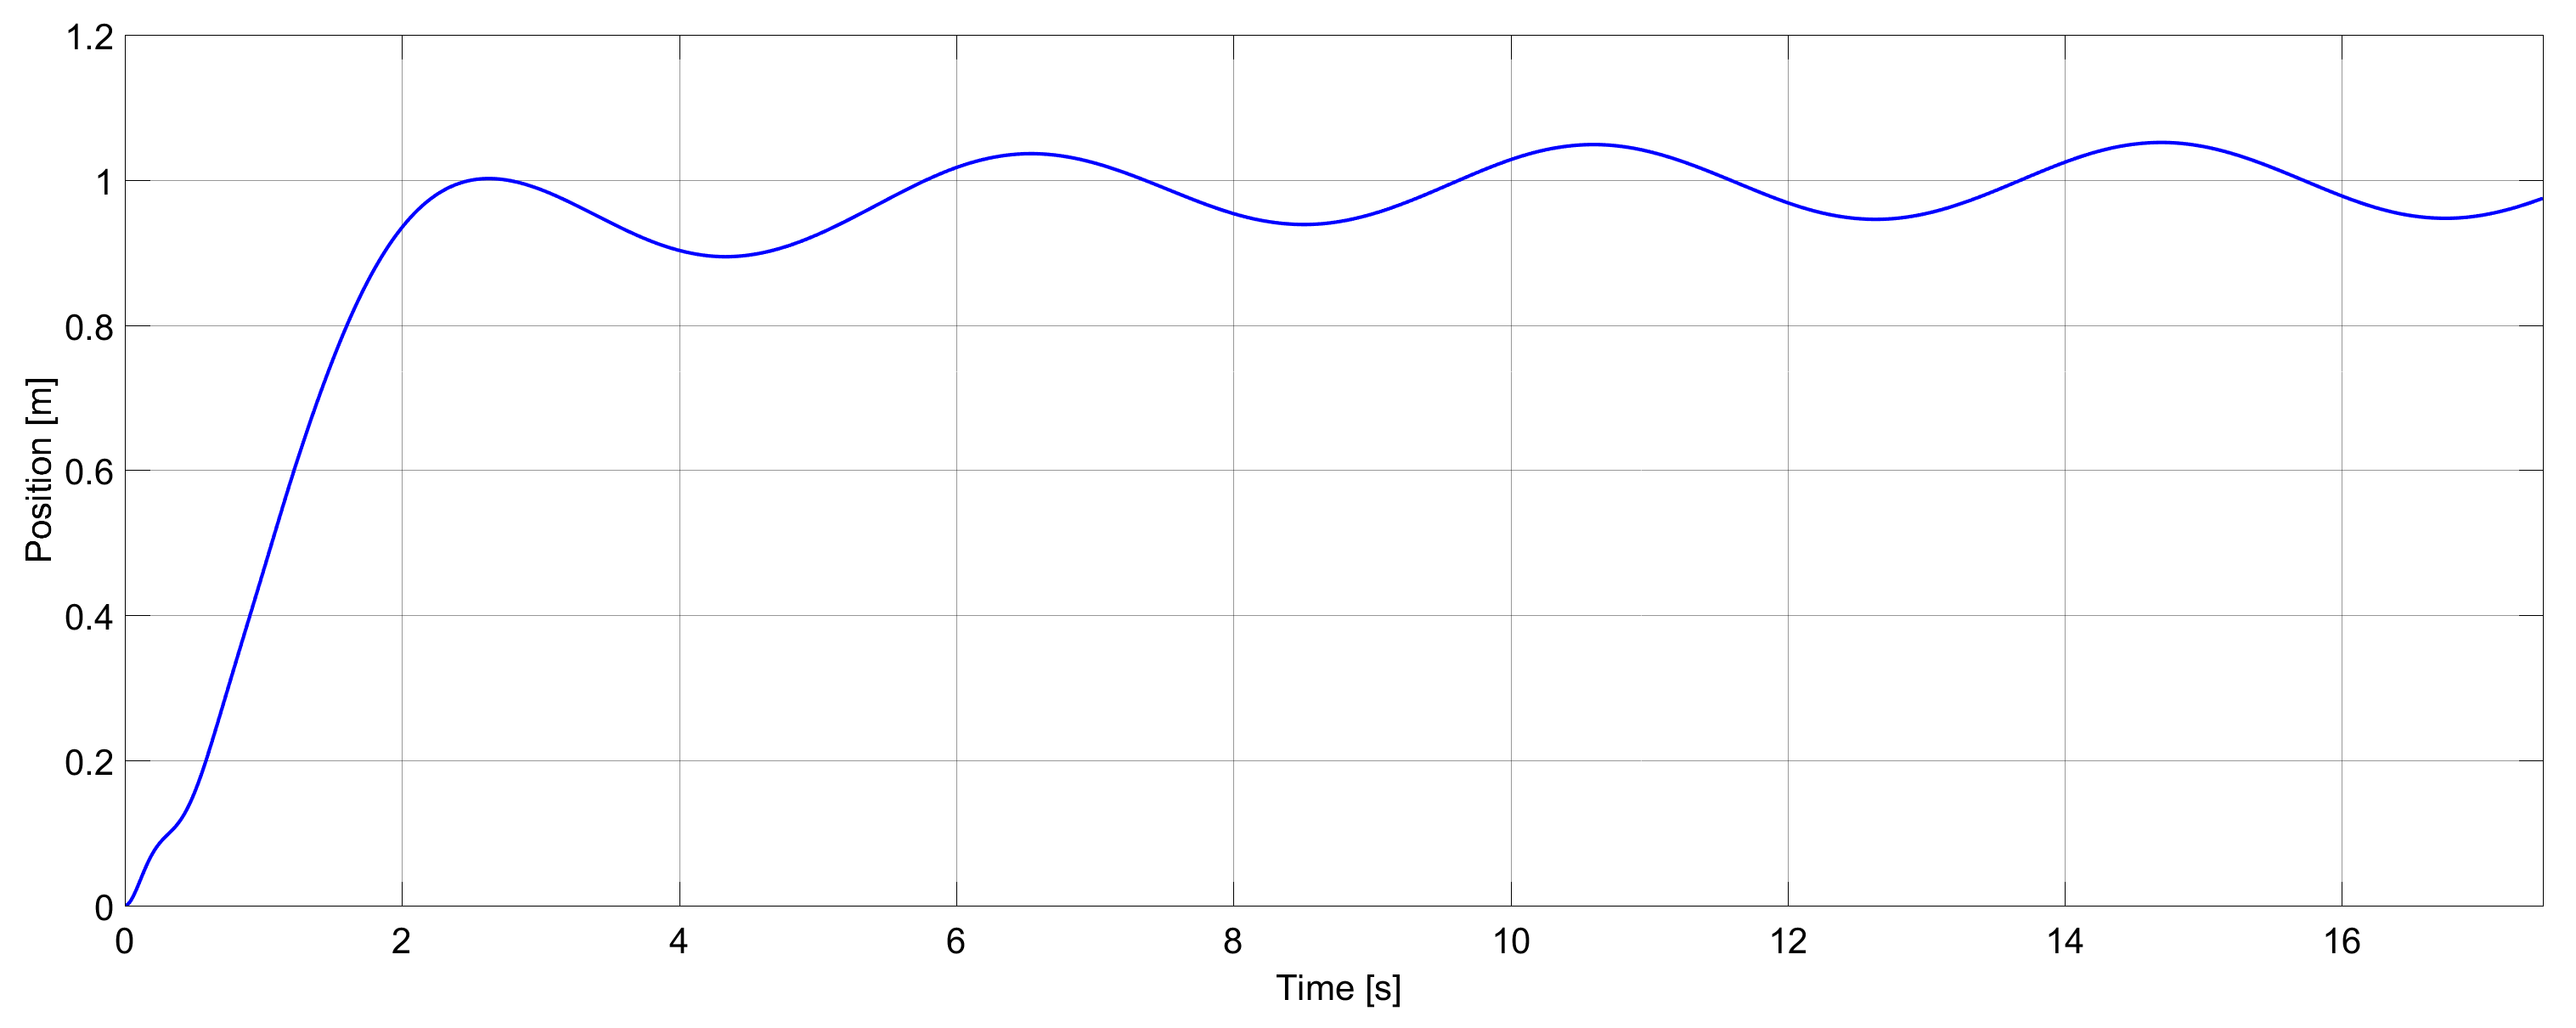
\includegraphics[width=0.8\textwidth]{Billeder/Thomas/100mA}
\end{figure}
\end{frame}


%\subsection{Trolley og pendul model}
% \begin{frame}{Regulator}{Block diagram}


%\begin{columns}[T]
% \begin{column}{.35\textwidth}

%   \begin{itemize}
%     \item<1-> Trolley
%     \vspace{0.8cm}
%     \item<2-> Electromagnetic head 
%     \vspace{1.5cm}
%     \item<3-> Angle sensor
%   \end{itemize}
% \end{column}%
% \hfill%
%\begin{column}{.65\textwidth}

%\vspace{-0.9cm}
%\begin{figure}[H]
%  \centering
% \onslide<1->  \begin{subfigure}{0.98\textwidth}
%         \centering
%         \includegraphics[width=0.5\textwidth]{Billeder/Papilio_DUO}
%         \end{subfigure}

% \onslide<2-> \scalebox{0.8}{ \begin{subfigure}{0.98\textwidth}
%         \centering
%         \begin{figure}[H]

%         \onslide<2-> \scalebox{0.7}{\input{Billeder/Thomas/regulatorblock3.ralf}}
%         \end{figure

%         }

%       \vspace{0.2cm}

%         \begin{figure}[H]

%         \onslide<3-> \scalebox{0.7}{\input{Billeder/Thomas/regulatorblock3.ralf}}
%         \end{figure

%         }




% \onslide<3->  \begin{subfigure}{0.98\textwidth}
%         \centering
%         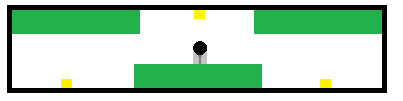
\includegraphics[width=0.5\textwidth]{Billeder/AngleSensor}
%         \end{subfigure}     
% \end{figure}

%\end{column}
%\end{columns}

%\end{frame}

%       \item<1->[] {
%               \begin{figure}[H]
%               \centering
%               \scalebox{0.65}{\input{Billeder/Thomas/regulatorblock3.ralf}}
%               \end{figure}
%       }
%     \end{itemize}           
%   \end{minipage}
%   \\

% %  \input{Billeder/Thomas/regulatorblock3.ralf}
  
% %  \input{Billeder/Thomas/regulatorblock4.ralf}
	  
%   \centering
%   \begin{minipage}[t]{0.75\linewidth}
%     \begin{itemize}
%       \item<1->[] {
%               \begin{figure}[H]
%               \centering
%               \scalebox{0.65}{\input{Billeder/Thomas/regulatorblock4.ralf}}
%               \end{figure}
%       }
%     \end{itemize}           
%   \end{minipage}
%   \\
  
% 	\centering   
%   \begin{minipage}[t]{0.55\linewidth}
    
%     \begin{itemize}
%       \item<1->[] {
%               \begin{figure}[H]
%               \centering
%               \scalebox{0.65}{\input{Billeder/Thomas/regulatorblocky.ralf}}
%               \end{figure}
%       }
%     \end{itemize}           
%   \end{minipage}
  
  
%\end{frame} 
%%%%%%%%%%%%%%%%
%\section{Implementering}
%%%%%%%%%%%% MID WAY AGENDA %%%%%%%%%%%%%%
\begin{frame}<beamer>
\frametitle{Ralf Victor Lømand Ravgård Christiansen}
\tableofcontents[currentsection]
\end{frame}
%%%%%%%%%%%% MID WAY AGENDA %%%%%%%%%%%%%%

%%%%%%%%%%%%%%%%%%%%%%%%%%%%%%%%%%%%%%%%%%%%%%%%%%%%%
%%%%%%%%%%%%%%%%%%%Implementering%%%%%%%%%%%%%%%%%%%%
%%%%%%%%%%%%%%%%%%%%%%%%%%%%%%%%%%%%%%%%%%%%%%%%%%%%%

%%%%%%%%%%%%%%%%%System Blokke%%%%%%%%%%%%%%%%%%%%%%%
\subsection{System blokke}
\begin{frame}{Implementering}{System blokke}
\vspace{1.5cm}
\begin{figure}[H]
  \centering
  \scalebox{0.75}{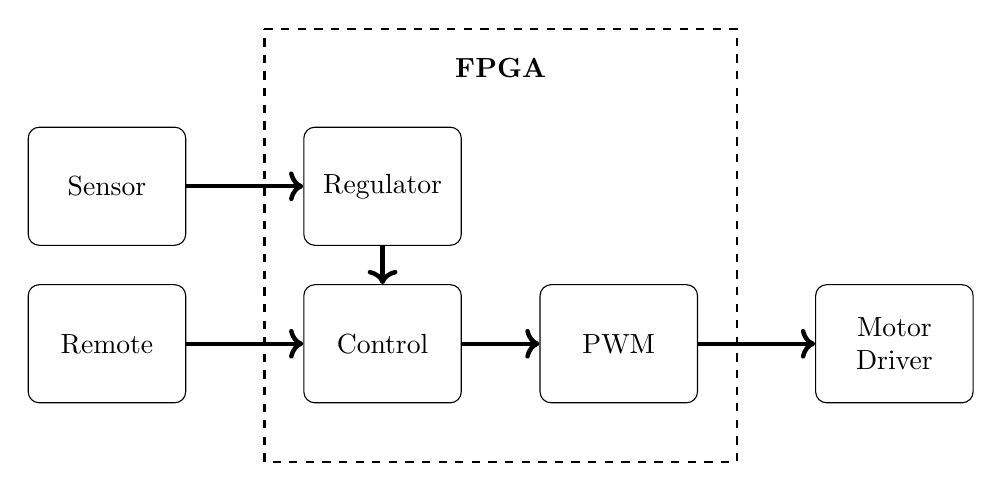
\begin{tikzpicture}
%Peripheral
\node[fill = white,box] (Sensor) at (0,0) {Sensor};
\node[fill = white,box] (RC) at ($(0,-2)+(Sensor)$) {Remote};
%FPGA
\node[fill = white,box] (Reg) at ($(3.5,0)+(Sensor)$) {Regulator};
\node[fill = white,box] (Cont) at ($(0,-2)+(Reg)$) {Control};
\node[fill = white,box] (PWM) at ($(3,0)+(Cont)$) {PWM};
\node[fill = white,box] (Mot) at ($(3.5,0)+(PWM)$) {Motor \\ Driver};

\draw[->, ultra thick] (RC) -- (Cont);
\draw[->, ultra thick] (Cont) -- (PWM);
\draw[->, ultra thick] (PWM) -- (Mot);
\draw[->, ultra thick] (Sensor) -- (Reg);
\draw[->, ultra thick] (Reg) -- (Cont);

\draw[thick,dashed] ($(-1.5,2)+(Reg)$) -- ($(1.5,4)+(PWM)$) -- ($(1.5,-1.5)+(PWM)$) -- ($(-1.5,-1.5)+(Cont)$) -- ($(-1.5,2)+(Reg)$);
\node[] at ($(1.5,1.5)+(Reg)$) {\textbf{FPGA}};
\end{tikzpicture}%}
\end{figure}

\end{frame}

%%%%%%%%%%%%%%%%Sensorer%%%%%%%%%%%%%%%%%%%%%%%%%%%
\subsection{Sensor}
\begin{frame}{Implementering}{Sensor}

  \begin{itemize}
    \item<1-> Tre sensorer
    \item<2-> Sensor støj
    \item<3-> 30. ordens FIR filter med Hamming vindue
  \end{itemize}

\begin{figure}[H]
  \centering
  \onslide<2-> \scalebox{0.7}{% This file was created by matlab2tikz.
%
%The latest updates can be retrieved from
%  http://www.mathworks.com/matlabcentral/fileexchange/22022-matlab2tikz-matlab2tikz
%where you can also make suggestions and rate matlab2tikz.
%
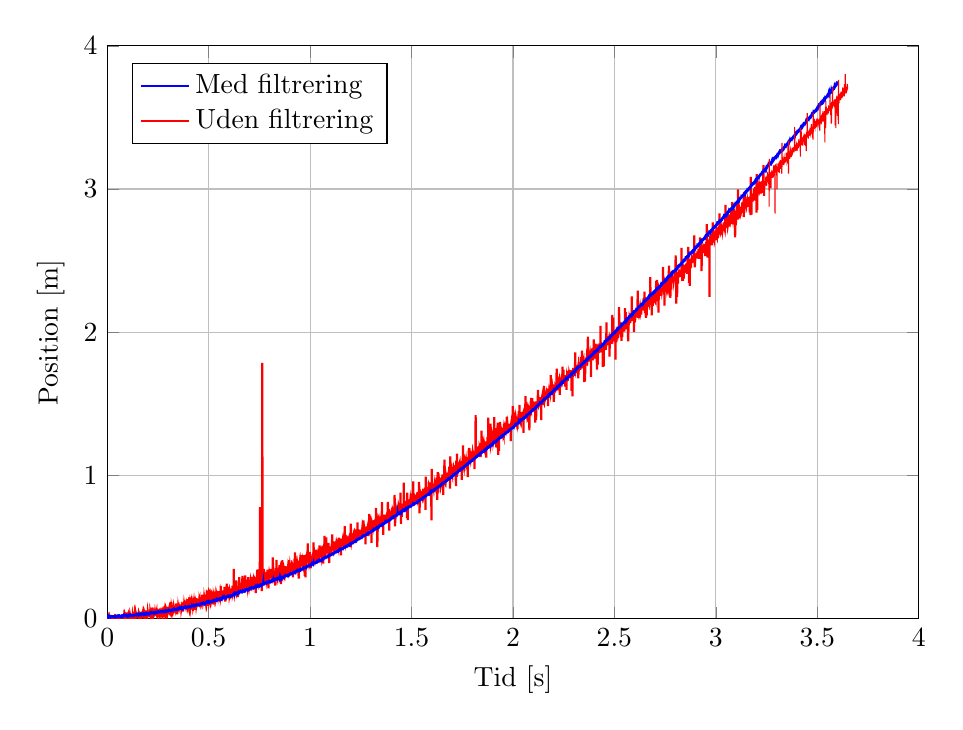
\begin{tikzpicture}

\begin{axis}[%
width=0.85\textwidth,
height=0.6\textwidth,
scale only axis,
separate axis lines,
every outer x axis line/.append style={black},
every x tick label/.append style={font=\color{black}},
xmin=0,
xmax=4,
xlabel={Tid [s]},
xmajorgrids,
every outer y axis line/.append style={black},
every y tick label/.append style={font=\color{black}},
ymin=0,
ymax=4,
ylabel={Position [m]},
ymajorgrids,
legend style={at={(0.03,0.97)},anchor=north west,legend cell align=left,align=left,fill=white},
axis background/.style={fill=white},
]
\addplot [color=blue,solid, thick]
  table[row sep=crcr]{%
3.240000000324	3.132\\
3.24081000032408	3.1308\\
3.24162000032416	3.1356\\
3.24243000032424	3.1392\\
3.24324000032432	3.1392\\
3.24405000032441	3.138\\
3.24486000032449	3.1356\\
3.24567000032457	3.1416\\
3.24648000032465	3.1464\\
3.24729000032473	3.1488\\
3.24810000032481	3.1464\\
3.24891000032489	3.1428\\
3.24972000032497	3.1476\\
3.25053000032505	3.1524\\
3.25134000032513	3.1548\\
3.25215000032521	3.1524\\
3.2529600003253	3.1512\\
3.25377000032538	3.1536\\
3.25458000032546	3.1584\\
3.25539000032554	3.162\\
3.25620000032562	3.1608\\
3.2570100003257	3.1584\\
3.25782000032578	3.1596\\
3.25863000032586	3.1632\\
3.25944000032594	3.1692\\
3.26025000032603	3.1668\\
3.26106000032611	3.1656\\
3.26187000032619	3.1644\\
3.26268000032627	3.1716\\
3.26349000032635	3.1752\\
3.26430000032643	3.174\\
3.26511000032651	3.1716\\
3.26592000032659	3.1716\\
3.26673000032667	3.1764\\
3.26754000032675	3.1812\\
3.26835000032683	3.1824\\
3.26916000032692	3.18\\
3.269970000327	3.1788\\
3.27078000032708	3.1824\\
3.27159000032716	3.1872\\
3.27240000032724	3.1884\\
3.27321000032732	3.186\\
3.2740200003274	3.1836\\
3.27483000032748	3.1884\\
3.27564000032756	3.1944\\
3.27645000032765	3.198\\
3.27726000032773	3.1932\\
3.27807000032781	3.192\\
3.27888000032789	3.1956\\
3.27969000032797	3.2016\\
3.28050000032805	3.204\\
3.28131000032813	3.2028\\
3.28212000032821	3.1992\\
3.28293000032829	3.2016\\
3.28374000032837	3.2064\\
3.28455000032845	3.2112\\
3.28536000032854	3.21\\
3.28617000032862	3.2064\\
3.2869800003287	3.2088\\
3.28779000032878	3.2136\\
3.28860000032886	3.216\\
3.28941000032894	3.216\\
3.29022000032902	3.2124\\
3.2910300003291	3.2136\\
3.29184000032918	3.2184\\
3.29265000032927	3.2232\\
3.29346000032935	3.2232\\
3.29427000032943	3.2208\\
3.29508000032951	3.2196\\
3.29589000032959	3.2244\\
3.29670000032967	3.2292\\
3.29751000032975	3.2292\\
3.29832000032983	3.2268\\
3.29913000032991	3.2256\\
3.29994000032999	3.2304\\
3.30075000033007	3.2352\\
3.30156000033016	3.2376\\
3.30237000033024	3.2352\\
3.30318000033032	3.234\\
3.3039900003304	3.2364\\
3.30480000033048	3.2424\\
3.30561000033056	3.2436\\
3.30642000033064	3.2424\\
3.30723000033072	3.2388\\
3.3080400003308	3.2424\\
3.30885000033088	3.2484\\
3.30966000033097	3.2508\\
3.31047000033105	3.2484\\
3.31128000033113	3.2472\\
3.31209000033121	3.2472\\
3.31290000033129	3.2544\\
3.31371000033137	3.258\\
3.31452000033145	3.2556\\
3.31533000033153	3.2532\\
3.31614000033161	3.2544\\
3.3169500003317	3.2604\\
3.31776000033178	3.264\\
3.31857000033186	3.2628\\
3.31938000033194	3.2592\\
3.32019000033202	3.2592\\
3.3210000003321	3.2652\\
3.32181000033218	3.27\\
3.32262000033226	3.27\\
3.32343000033234	3.2664\\
3.32424000033242	3.2664\\
3.3250500003325	3.27\\
3.32586000033259	3.276\\
3.32667000033267	3.276\\
3.32748000033275	3.2736\\
3.32829000033283	3.2724\\
3.32910000033291	3.276\\
3.32991000033299	3.2832\\
3.33072000033307	3.2832\\
3.33153000033315	3.2808\\
3.33234000033323	3.2796\\
3.33315000033332	3.2832\\
3.3339600003334	3.2892\\
3.33477000033348	3.2904\\
3.33558000033356	3.288\\
3.33639000033364	3.2856\\
3.33720000033372	3.288\\
3.3380100003338	3.294\\
3.33882000033388	3.2976\\
3.33963000033396	3.2952\\
3.34044000033404	3.2928\\
3.34125000033412	3.294\\
3.34206000033421	3.3\\
3.34287000033429	3.3048\\
3.34368000033437	3.3036\\
3.34449000033445	3.3\\
3.34530000033453	3.3012\\
3.34611000033461	3.306\\
3.34692000033469	3.3096\\
3.34773000033477	3.3108\\
3.34854000033485	3.306\\
3.34935000033494	3.3084\\
3.35016000033502	3.312\\
3.3509700003351	3.3168\\
3.35178000033518	3.3168\\
3.35259000033526	3.3144\\
3.35340000033534	3.3132\\
3.35421000033542	3.3192\\
3.3550200003355	3.3228\\
3.35583000033558	3.3252\\
3.35664000033566	3.3216\\
3.35745000033574	3.3204\\
3.35826000033583	3.3252\\
3.35907000033591	3.33\\
3.35988000033599	3.33\\
3.36069000033607	3.3288\\
3.36150000033615	3.3264\\
3.36231000033623	3.33\\
3.36312000033631	3.3348\\
3.36393000033639	3.3384\\
3.36474000033647	3.3324\\
3.36555000033656	3.3336\\
3.36636000033664	3.336\\
3.36717000033672	3.342\\
3.3679800003368	3.3444\\
3.36879000033688	3.3432\\
3.36960000033696	3.3408\\
3.37041000033704	3.342\\
3.37122000033712	3.348\\
3.3720300003372	3.3516\\
3.37284000033728	3.3516\\
3.37365000033736	3.3492\\
3.37446000033745	3.348\\
3.37527000033753	3.354\\
3.37608000033761	3.3564\\
3.37689000033769	3.3576\\
3.37770000033777	3.354\\
3.37851000033785	3.3552\\
3.37932000033793	3.3588\\
3.38013000033801	3.3636\\
3.38094000033809	3.3648\\
3.38175000033818	3.3612\\
3.38256000033826	3.36\\
3.38337000033834	3.3648\\
3.38418000033842	3.3708\\
3.3849900003385	3.372\\
3.38580000033858	3.3708\\
3.38661000033866	3.3696\\
3.38742000033874	3.3732\\
3.38823000033882	3.378\\
3.3890400003389	3.3792\\
3.38985000033898	3.3768\\
3.39066000033907	3.3744\\
3.39147000033915	3.3792\\
3.39228000033923	3.3852\\
3.39309000033931	3.3876\\
3.39390000033939	3.3852\\
3.39471000033947	3.3828\\
3.39552000033955	3.384\\
3.39633000033963	3.39\\
3.39714000033971	3.3924\\
3.3979500003398	3.3912\\
3.39876000033988	3.3888\\
3.39957000033996	3.3912\\
3.40038000034004	3.3948\\
3.40119000034012	3.3996\\
3.4020000003402	3.3984\\
3.40281000034028	3.396\\
3.40362000034036	3.396\\
3.40443000034044	3.402\\
3.40524000034052	3.4068\\
3.4060500003406	3.4068\\
3.40686000034069	3.4032\\
3.40767000034077	3.4032\\
3.40848000034085	3.4068\\
3.40929000034093	3.4128\\
3.41010000034101	3.4128\\
3.41091000034109	3.4104\\
3.41172000034117	3.4092\\
3.41253000034125	3.4128\\
3.41334000034133	3.42\\
3.41415000034142	3.4212\\
3.4149600003415	3.4176\\
3.41577000034158	3.4164\\
3.41658000034166	3.42\\
3.41739000034174	3.4248\\
3.41820000034182	3.4284\\
3.4190100003419	3.426\\
3.41982000034198	3.4224\\
3.42063000034206	3.4248\\
3.42144000034214	3.432\\
3.42225000034222	3.4344\\
3.42306000034231	3.432\\
3.42387000034239	3.4296\\
3.42468000034247	3.432\\
3.42549000034255	3.4368\\
3.42630000034263	3.4416\\
3.42711000034271	3.4404\\
3.42792000034279	3.4368\\
3.42873000034287	3.4392\\
3.42954000034295	3.444\\
3.43035000034303	3.4488\\
3.43116000034312	3.4476\\
3.4319700003432	3.4452\\
3.43278000034328	3.4452\\
3.43359000034336	3.45\\
3.43440000034344	3.4548\\
3.43521000034352	3.4536\\
3.4360200003436	3.4512\\
3.43683000034368	3.4512\\
3.43764000034376	3.456\\
3.43845000034385	3.462\\
3.43926000034393	3.462\\
3.44007000034401	3.4596\\
3.44088000034409	3.4584\\
3.44169000034417	3.462\\
3.44250000034425	3.4668\\
3.44331000034433	3.4704\\
3.44412000034441	3.4668\\
3.44493000034449	3.4656\\
3.44574000034457	3.4668\\
3.44655000034465	3.474\\
3.44736000034474	3.4776\\
3.44817000034482	3.474\\
3.4489800003449	3.4728\\
3.44979000034498	3.4752\\
3.45060000034506	3.4812\\
3.45141000034514	3.4836\\
3.45222000034522	3.4824\\
3.4530300003453	3.48\\
3.45384000034538	3.4812\\
3.45465000034547	3.4872\\
3.45546000034555	3.492\\
3.45627000034563	3.4908\\
3.45708000034571	3.4884\\
3.45789000034579	3.4872\\
3.45870000034587	3.4932\\
3.45951000034595	3.498\\
3.46032000034603	3.498\\
3.46113000034611	3.4944\\
3.46194000034619	3.4944\\
3.46275000034627	3.4992\\
3.46356000034636	3.504\\
3.46437000034644	3.5052\\
3.46518000034652	3.5028\\
3.4659900003466	3.5016\\
3.46680000034668	3.5064\\
3.46761000034676	3.5112\\
3.46842000034684	3.5124\\
3.46923000034692	3.51\\
3.470040000347	3.5088\\
3.47085000034709	3.5124\\
3.47166000034717	3.516\\
3.47247000034725	3.5196\\
3.47328000034733	3.5172\\
3.47409000034741	3.516\\
3.47490000034749	3.5184\\
3.47571000034757	3.5256\\
3.47652000034765	3.5268\\
3.47733000034773	3.5256\\
3.47814000034781	3.5232\\
3.47895000034789	3.5244\\
3.47976000034798	3.5304\\
3.48057000034806	3.5352\\
3.48138000034814	3.5328\\
3.48219000034822	3.5304\\
3.4830000003483	3.5316\\
3.48381000034838	3.5376\\
3.48462000034846	3.5412\\
3.48543000034854	3.5412\\
3.48624000034862	3.5376\\
3.48705000034871	3.5376\\
3.48786000034879	3.5424\\
3.48867000034887	3.5472\\
3.48948000034895	3.5484\\
3.49029000034903	3.5448\\
3.49110000034911	3.5448\\
3.49191000034919	3.5496\\
3.49272000034927	3.5544\\
3.49353000034935	3.5556\\
3.49434000034943	3.552\\
3.49515000034951	3.5508\\
3.4959600003496	3.5556\\
3.49677000034968	3.5604\\
3.49758000034976	3.5628\\
3.49839000034984	3.5604\\
3.49920000034992	3.5592\\
3.50001000035	3.5628\\
3.50082000035008	3.5676\\
3.50163000035016	3.57\\
3.50244000035024	3.5676\\
3.50325000035033	3.5652\\
3.50406000035041	3.5688\\
3.50487000035049	3.5748\\
3.50568000035057	3.5784\\
3.50649000035065	3.576\\
3.50730000035073	3.5736\\
3.50811000035081	3.5748\\
3.50892000035089	3.5808\\
3.50973000035097	3.5844\\
3.51054000035105	3.5832\\
3.51135000035113	3.5808\\
3.51216000035122	3.582\\
3.5129700003513	3.5856\\
3.51378000035138	3.5916\\
3.51459000035146	3.5904\\
3.51540000035154	3.5868\\
3.51621000035162	3.588\\
3.5170200003517	3.5928\\
3.51783000035178	3.6\\
3.51864000035186	3.5988\\
3.51945000035195	3.5928\\
3.52026000035203	3.594\\
3.52107000035211	3.6\\
3.52188000035219	3.6048\\
3.52269000035227	3.6036\\
3.52350000035235	3.6036\\
3.52431000035243	3.6024\\
3.52512000035251	3.6072\\
3.52593000035259	3.6132\\
3.52674000035267	3.612\\
3.52755000035275	3.612\\
3.52836000035284	3.6096\\
3.52917000035292	3.6132\\
3.529980000353	3.618\\
3.53079000035308	3.6216\\
3.53160000035316	3.6192\\
3.53241000035324	3.6168\\
3.53322000035332	3.6204\\
3.5340300003534	3.6264\\
3.53484000035348	3.6288\\
3.53565000035357	3.6264\\
3.53646000035365	3.624\\
3.53727000035373	3.6228\\
3.53808000035381	3.6312\\
3.53889000035389	3.6372\\
3.53970000035397	3.636\\
3.54051000035405	3.6324\\
3.54132000035413	3.6336\\
3.54213000035421	3.6384\\
3.54294000035429	3.642\\
3.54375000035437	3.6432\\
3.54456000035446	3.6396\\
3.54537000035454	3.6396\\
3.54618000035462	3.6444\\
3.5469900003547	3.648\\
3.54780000035478	3.6504\\
3.54861000035486	3.6468\\
3.54942000035494	3.648\\
3.55023000035502	3.6504\\
3.5510400003551	3.654\\
3.55185000035518	3.6564\\
3.55266000035527	3.6528\\
3.55347000035535	3.6528\\
3.55428000035543	3.6564\\
3.55509000035551	3.66\\
3.55590000035559	3.666\\
3.55671000035567	3.6612\\
3.55752000035575	3.6576\\
3.55833000035583	3.6636\\
3.55914000035591	3.6672\\
3.559950000356	3.6732\\
3.56076000035608	3.6672\\
3.56157000035616	3.666\\
3.56238000035624	3.6684\\
3.56319000035632	3.6756\\
3.5640000003564	3.678\\
3.56481000035648	3.6768\\
3.56562000035656	3.672\\
3.56643000035664	3.6732\\
3.56724000035672	3.6816\\
3.5680500003568	3.6876\\
3.56886000035689	3.6816\\
3.56967000035697	3.6804\\
3.57048000035705	3.6792\\
3.57129000035713	3.6876\\
3.57210000035721	3.6924\\
3.57291000035729	3.6936\\
3.57372000035737	3.69\\
3.57453000035745	3.6888\\
3.57534000035753	3.6936\\
3.57615000035762	3.6996\\
3.5769600003577	3.6984\\
3.57777000035778	3.696\\
3.57858000035786	3.696\\
3.57939000035794	3.6996\\
3.58020000035802	3.7044\\
3.5810100003581	3.7068\\
3.58182000035818	3.702\\
3.58263000035826	3.7032\\
3.58344000035834	3.7068\\
3.58425000035842	3.7128\\
3.58506000035851	3.7188\\
3.58587000035859	3.7152\\
3.58668000035867	3.7116\\
3.58749000035875	3.714\\
3.58830000035883	3.7212\\
3.58911000035891	3.7236\\
3.58992000035899	3.7224\\
3.59073000035907	3.7188\\
3.59154000035915	3.72\\
3.59235000035924	3.726\\
3.59316000035932	3.7308\\
3.5939700003594	3.7296\\
3.59478000035948	3.726\\
3.59559000035956	3.7272\\
3.59640000035964	3.732\\
3.59721000035972	3.738\\
3.5980200003598	3.7368\\
3.59883000035988	3.7332\\
3.59964000035996	3.7344\\
3.60045000036004	3.7392\\
3.60126000036013	3.744\\
3.60207000036021	3.744\\
};
\addplot [color=red,solid, thick]
  table[row sep=crcr]{%
0	0.00600000000000001\\
0.000810000000081	0.00480000000000003\\
0.001620000000162	0.00480000000000003\\
0.002430000000243	0.00480000000000003\\
0.003240000000324	0.00480000000000003\\
0.004050000000405	0.00480000000000003\\
0.004860000000486	0.00480000000000003\\
0.005670000000567	0.00600000000000001\\
0.006480000000648	-0.012\\
0.007290000000729	-0.00239999999999996\\
0.00810000000081	0.00120000000000003\\
0.008910000000891	0.0108\\
0.009720000000972	0.00720000000000004\\
0.010530000001053	0.0216\\
0.011340000001134	-0.00359999999999999\\
0.012150000001215	0\\
0.012960000001296	0.0108\\
0.013770000001377	0.00720000000000004\\
0.014580000001458	0.00480000000000003\\
0.015390000001539	-0.00839999999999996\\
0.01620000000162	0.0192\\
0.017010000001701	0.0108\\
0.017820000001782	0.00720000000000004\\
0.018630000001863	0.00480000000000003\\
0.019440000001944	0\\
0.020250000002025	0.00840000000000002\\
0.021060000002106	0.0108\\
0.021870000002187	0.0108\\
0.022680000002268	0.00720000000000004\\
0.023490000002349	-0.012\\
0.02430000000243	-0.00119999999999998\\
0.025110000002511	0.0108\\
0.025920000002592	0.00960000000000003\\
0.026730000002673	0.00480000000000003\\
0.027540000002754	0.00240000000000001\\
0.028350000002835	0.00120000000000003\\
0.029160000002916	0.0108\\
0.029970000002997	0.0108\\
0.030780000003078	0.00720000000000004\\
0.031590000003159	0\\
0.03240000000324	-0.00479999999999997\\
0.033210000003321	0.0108\\
0.034020000003402	0.0108\\
0.034830000003483	0.0108\\
0.035640000003564	-0.0204\\
0.036450000003645	-0.00119999999999998\\
0.037260000003726	0.0108\\
0.038070000003807	0.0108\\
0.038880000003888	0.00960000000000003\\
0.039690000003969	0.0324\\
0.04050000000405	0.00120000000000003\\
0.041310000004131	-0.00359999999999999\\
0.042120000004212	0.0108\\
0.042930000004293	0.00960000000000003\\
0.043740000004374	0.00480000000000003\\
0.044550000004455	-0.00719999999999998\\
0.045360000004536	0.0108\\
0.046170000004617	0.0108\\
0.046980000004698	0.00960000000000003\\
0.047790000004779	0.00720000000000004\\
0.04860000000486	0\\
0.049410000004941	-0.00119999999999998\\
0.050220000005022	0.0108\\
0.051030000005103	0.0108\\
0.051840000005184	0.00720000000000004\\
0.052650000005265	-0.00479999999999997\\
0.053460000005346	0.00120000000000003\\
0.054270000005427	0.0108\\
0.055080000005508	0.0108\\
0.055890000005589	0.0108\\
0.05670000000567	-0.00239999999999996\\
0.057510000005751	0.00120000000000003\\
0.058320000005832	0.0108\\
0.059130000005913	0.0108\\
0.059940000005994	0.0108\\
0.060750000006075	0.0108\\
0.061560000006156	-0.00239999999999996\\
0.062370000006237	0.0108\\
0.063180000006318	0.0108\\
0.063990000006399	0.00960000000000003\\
0.06480000000648	-0.018\\
0.065610000006561	0.00120000000000003\\
0.066420000006642	0.00840000000000002\\
0.067230000006723	0.0108\\
0.068040000006804	0.0108\\
0.068850000006885	0.0216\\
0.069660000006966	0.00120000000000003\\
0.070470000007047	0.0192\\
0.071280000007128	0.0108\\
0.072090000007209	0.0108\\
0.07290000000729	0.012\\
0.073710000007371	0\\
0.074520000007452	0.03\\
0.075330000007533	0.0204\\
0.076140000007614	0.0108\\
0.076950000007695	0.00720000000000004\\
0.077760000007776	0.00120000000000003\\
0.078570000007857	-0.0276\\
0.079380000007938	0.0108\\
0.080190000008019	0.0108\\
0.0810000000081	0.0108\\
0.081810000008181	0.00240000000000001\\
0.082620000008262	0.00600000000000001\\
0.083430000008343	0.0192\\
0.084240000008424	0.0144\\
0.085050000008505	0.0108\\
0.085860000008586	-0.00599999999999995\\
0.086670000008667	0.00360000000000002\\
0.087480000008748	0.0204\\
0.088290000008829	0.0156\\
0.08910000000891	0.018\\
0.089910000008991	0.0144\\
0.090720000009072	0.00480000000000003\\
0.091530000009153	0.0204\\
0.092340000009234	0.0192\\
0.093150000009315	0.0108\\
0.093960000009396	-0.00719999999999998\\
0.094770000009477	0.00480000000000003\\
0.095580000009558	0.0204\\
0.096390000009639	0.018\\
0.09720000000972	0.018\\
0.098010000009801	0\\
0.098820000009882	0.00720000000000004\\
0.099630000009963	0.00120000000000003\\
0.100440000010044	0.0252\\
0.101250000010125	0.0156\\
0.102060000010206	0.0432\\
0.102870000010287	0.00120000000000003\\
0.103680000010368	0.0252\\
0.104490000010449	0.0252\\
0.10530000001053	0.0168\\
0.106110000010611	0.0108\\
0.106920000010692	0.00120000000000003\\
0.107730000010773	-0.0276\\
0.108540000010854	0.0204\\
0.109350000010935	0.0168\\
0.110160000011016	0.0192\\
0.110970000011097	0.00960000000000003\\
0.111780000011178	0.0108\\
0.112590000011259	0.0252\\
0.11340000001134	0.0192\\
0.114210000011421	0.0144\\
0.115020000011502	0.00240000000000001\\
0.115830000011583	0.00600000000000001\\
0.116640000011664	0.0108\\
0.117450000011745	0.0192\\
0.118260000011826	0.0204\\
0.119070000011907	0.00960000000000003\\
0.119880000011988	0.00960000000000003\\
0.120690000012069	0.0192\\
0.12150000001215	0.0204\\
0.122310000012231	0.0204\\
0.123120000012312	0.00720000000000004\\
0.123930000012393	0.00960000000000003\\
0.124740000012474	0.0108\\
0.125550000012555	0.0252\\
0.126360000012636	0.018\\
0.127170000012717	-0.00839999999999996\\
0.127980000012798	0.00720000000000004\\
0.128790000012879	0.0108\\
0.12960000001296	0.024\\
0.130410000013041	0.024\\
0.131220000013122	0.0492\\
0.132030000013203	0.00840000000000002\\
0.132840000013284	0.0444\\
0.133650000013365	0.0288\\
0.134460000013446	0.0204\\
0.135270000013527	0.018\\
0.136080000013608	0.00480000000000003\\
0.136890000013689	-0.018\\
0.13770000001377	0.03\\
0.138510000013851	0.024\\
0.139320000013932	0.024\\
0.140130000014013	0.012\\
0.140940000014094	0.00120000000000003\\
0.141750000014175	0.03\\
0.142560000014256	0.024\\
0.143370000014337	0.0204\\
0.144180000014418	0.0108\\
0.144990000014499	0.0108\\
0.14580000001458	0.0204\\
0.146610000014661	0.0276\\
0.147420000014742	0.0252\\
0.148230000014823	0.0108\\
0.149040000014904	0.0108\\
0.149850000014985	0.0396\\
0.150660000015066	0.0288\\
0.151470000015147	0.0264\\
0.152280000015228	0.0264\\
0.153090000015309	0.0108\\
0.15390000001539	0.0204\\
0.154710000015471	0.03\\
0.155520000015552	0.024\\
0.156330000015633	-0.00479999999999997\\
0.157140000015714	0.00960000000000003\\
0.157950000015795	0.0108\\
0.158760000015876	0.03\\
0.159570000015957	0.0264\\
0.160380000016038	0.0408\\
0.161190000016119	0.0144\\
0.1620000000162	0.0432\\
0.162810000016281	0.03\\
0.163620000016362	0.0288\\
0.164430000016443	0.0288\\
0.165240000016524	0.00960000000000003\\
0.166050000016605	0.0492\\
0.166860000016686	0.03\\
0.167670000016767	0.0264\\
0.168480000016848	0.024\\
0.169290000016929	0.0144\\
0.17010000001701	0.0192\\
0.170910000017091	0.03\\
0.171720000017172	0.0336\\
0.172530000017253	0.0252\\
0.173340000017334	0.0192\\
0.174150000017415	0.018\\
0.174960000017496	0.03\\
0.175770000017577	0.03\\
0.176580000017658	0.0276\\
0.177390000017739	0.00720000000000004\\
0.17820000001782	0.0204\\
0.179010000017901	0.0396\\
0.179820000017982	0.0348\\
0.180630000018063	0.0276\\
0.181440000018144	0.0312\\
0.182250000018225	0.018\\
0.183060000018306	0.0396\\
0.183870000018387	0.0348\\
0.184680000018468	0.0312\\
0.185490000018549	0.00960000000000003\\
0.18630000001863	0.0168\\
0.187110000018711	0.0252\\
0.187920000018792	0.0372\\
0.188730000018873	0.0348\\
0.189540000018954	0.0168\\
0.190350000019035	0.0204\\
0.191160000019116	0.0492\\
0.191970000019197	0.0384\\
0.192780000019278	0.0384\\
0.193590000019359	0.0576\\
0.19440000001944	0.0192\\
0.195210000019521	0.00480000000000003\\
0.196020000019602	0.0348\\
0.196830000019683	0.0348\\
0.197640000019764	0.0312\\
0.198450000019845	0.0192\\
0.199260000019926	0.0276\\
0.200070000020007	0.0444\\
0.200880000020088	0.036\\
0.201690000020169	0.0312\\
0.20250000002025	0.0288\\
0.203310000020331	0.0276\\
0.204120000020412	0.0396\\
0.204930000020493	0.0384\\
0.205740000020574	0.0372\\
0.206550000020655	0.0144\\
0.207360000020736	0.0276\\
0.208170000020817	0.0396\\
0.208980000020898	0.0432\\
0.209790000020979	0.0348\\
0.21060000002106	0.0288\\
0.211410000021141	0.0252\\
0.212220000021222	0.0492\\
0.213030000021303	0.0432\\
0.213840000021384	0.036\\
0.214650000021465	0.0312\\
0.215460000021546	0.024\\
0.216270000021627	0.03\\
0.217080000021708	0.0492\\
0.217890000021789	0.0384\\
0.21870000002187	0.00240000000000001\\
0.219510000021951	0.024\\
0.220320000022032	0.0588\\
0.221130000022113	0.0396\\
0.221940000022194	0.042\\
0.222750000022275	0.0792\\
0.223560000022356	0.0288\\
0.224370000022437	-0.0132\\
0.225180000022518	0.0444\\
0.225990000022599	0.0456\\
0.22680000002268	0.036\\
0.227610000022761	0.0216\\
0.228420000022842	0.0252\\
0.229230000022923	0.0468\\
0.230040000023004	0.0456\\
0.230850000023085	0.0384\\
0.231660000023166	0.0336\\
0.232470000023247	0.0372\\
0.233280000023328	0.0444\\
0.234090000023409	0.042\\
0.23490000002349	0.0432\\
0.235710000023571	0.0288\\
0.236520000023652	0.03\\
0.237330000023733	0.0492\\
0.238140000023814	0.0444\\
0.238950000023895	0.042\\
0.239760000023976	0.0264\\
0.240570000024057	0.0372\\
0.241380000024138	0.0492\\
0.242190000024219	0.0492\\
0.2430000000243	0.0432\\
0.243810000024381	0.0492\\
0.244620000024462	0.0336\\
0.245430000024543	0.03\\
0.246240000024624	0.0492\\
0.247050000024705	0.0468\\
0.247860000024786	0.0108\\
0.248670000024867	0.0336\\
0.249480000024948	0.0684\\
0.250290000025029	0.0492\\
0.25110000002511	0.048\\
0.251910000025191	0.0684\\
0.252720000025272	0.036\\
0.253530000025353	0.0684\\
0.254340000025434	0.0492\\
0.255150000025515	0.048\\
0.255960000025596	0.048\\
0.256770000025677	0.036\\
0.257580000025758	0.0444\\
0.258390000025839	0.0588\\
0.25920000002592	0.0492\\
0.260010000026001	0.048\\
0.260820000026082	0.0384\\
0.261630000026163	0.0444\\
0.262440000026244	0.0576\\
0.263250000026325	0.0564\\
0.264060000026406	0.0492\\
0.264870000026487	0.0456\\
0.265680000026568	0.0396\\
0.266490000026649	0.0492\\
0.26730000002673	0.0564\\
0.268110000026811	0.054\\
0.268920000026892	0.03\\
0.269730000026973	0.0396\\
0.270540000027054	0.0588\\
0.271350000027135	0.0588\\
0.272160000027216	0.0576\\
0.272970000027297	0.0576\\
0.273780000027378	0.0432\\
0.274590000027459	0.0492\\
0.27540000002754	0.0576\\
0.276210000027621	0.0552\\
0.277020000027702	0.0336\\
0.277830000027783	0.0444\\
0.278640000027864	0.0396\\
0.279450000027945	0.0588\\
0.280260000028026	0.0588\\
0.281070000028107	0.0384\\
0.281880000028188	0.0456\\
0.282690000028269	0.0204\\
0.28350000002835	0.066\\
0.284310000028431	0.0576\\
0.285120000028512	0.0888\\
0.285930000028593	0.0456\\
0.286740000028674	0.0396\\
0.287550000028755	0.0636\\
0.288360000028836	0.0588\\
0.289170000028917	0.0552\\
0.289980000028998	0.0432\\
0.290790000029079	0.0492\\
0.29160000002916	0.066\\
0.292410000029241	0.0624\\
0.293220000029322	0.0552\\
0.294030000029403	0.0576\\
0.294840000029484	0.0492\\
0.295650000029565	0.0636\\
0.296460000029646	0.0636\\
0.297270000029727	0.0588\\
0.298080000029808	0.0432\\
0.298890000029889	0.0492\\
0.29970000002997	0.0684\\
0.300510000030051	0.0672\\
0.301320000030132	0.06\\
0.302130000030213	0.0564\\
0.302940000030294	0.054\\
0.303750000030375	0.0636\\
0.304560000030456	0.0684\\
0.305370000030537	0.0612\\
0.306180000030618	0.0552\\
0.306990000030699	0.0528\\
0.30780000003078	0.0588\\
0.308610000030861	0.0684\\
0.309420000030942	0.0624\\
0.310230000031023	0.024\\
0.311040000031104	0.0492\\
0.311850000031185	0.078\\
0.312660000031266	0.0684\\
0.313470000031347	0.072\\
0.314280000031428	0.1152\\
0.315090000031509	0.0552\\
0.31590000003159	0.0588\\
0.316710000031671	0.078\\
0.317520000031752	0.0708\\
0.318330000031833	0.0624\\
0.319140000031914	0.0492\\
0.319950000031995	0.0588\\
0.320760000032076	0.0684\\
0.321570000032157	0.0672\\
0.322380000032238	0.0648\\
0.323190000032319	0.06\\
0.3240000000324	0.0624\\
0.324810000032481	0.0684\\
0.325620000032562	0.0768\\
0.326430000032643	0.0672\\
0.327240000032724	0.0552\\
0.328050000032805	0.0588\\
0.328860000032886	0.0828\\
0.329670000032967	0.078\\
0.330480000033048	0.0732\\
0.331290000033129	0.054\\
0.33210000003321	0.0624\\
0.332910000033291	0.0828\\
0.333720000033372	0.0744\\
0.334530000033453	0.0684\\
0.335340000033534	0.078\\
0.336150000033615	0.0588\\
0.336960000033696	0.078\\
0.337770000033777	0.078\\
0.338580000033858	0.0744\\
0.339390000033939	0.0348\\
0.34020000003402	0.0636\\
0.341010000034101	0.1068\\
0.341820000034182	0.078\\
0.342630000034263	0.0768\\
0.343440000034344	0.0984\\
0.344250000034425	0.0648\\
0.345060000034506	0.03\\
0.345870000034587	0.0876\\
0.346680000034668	0.0792\\
0.347490000034749	0.0792\\
0.34830000003483	0.06\\
0.349110000034911	0.0684\\
0.349920000034992	0.0852\\
0.350730000035073	0.078\\
0.351540000035154	0.078\\
0.352350000035235	0.0708\\
0.353160000035316	0.0684\\
0.353970000035397	0.078\\
0.354780000035478	0.0828\\
0.355590000035559	0.078\\
0.35640000003564	0.0708\\
0.357210000035721	0.0732\\
0.358020000035802	0.0972\\
0.358830000035883	0.0864\\
0.359640000035964	0.0828\\
0.360450000036045	0.0576\\
0.361260000036126	0.0732\\
0.362070000036207	0.0876\\
0.362880000036288	0.0876\\
0.363690000036369	0.0804\\
0.36450000003645	0.0924\\
0.365310000036531	0.0708\\
0.366120000036612	0.078\\
0.366930000036693	0.0876\\
0.367740000036774	0.084\\
0.368550000036855	0.0576\\
0.369360000036936	0.0684\\
0.370170000037017	0.1116\\
0.370980000037098	0.0972\\
0.371790000037179	0.0876\\
0.37260000003726	0.0744\\
0.373410000037341	0.0768\\
0.374220000037422	0.0492\\
0.375030000037503	0.0876\\
0.375840000037584	0.0876\\
0.376650000037665	0.1176\\
0.377460000037746	0.0732\\
0.378270000037827	0.0828\\
0.379080000037908	0.0972\\
0.379890000037989	0.0888\\
0.38070000003807	0.0888\\
0.381510000038151	0.072\\
0.382320000038232	0.0828\\
0.383130000038313	0.0876\\
0.383940000038394	0.0912\\
0.384750000038475	0.0924\\
0.385560000038556	0.0864\\
0.386370000038637	0.0828\\
0.387180000038718	0.0972\\
0.387990000038799	0.0936\\
0.38880000003888	0.0924\\
0.389610000038961	0.0684\\
0.390420000039042	0.0792\\
0.391230000039123	0.0876\\
0.392040000039204	0.0972\\
0.392850000039285	0.0912\\
0.393660000039366	0.0888\\
0.394470000039447	0.084\\
0.395280000039528	0.1068\\
0.396090000039609	0.1044\\
0.39690000003969	0.0972\\
0.397710000039771	0.0888\\
0.398520000039852	0.0816\\
0.399330000039933	0.1356\\
0.400140000040014	0.1008\\
0.400950000040095	0.0972\\
0.401760000040176	0.0588\\
0.402570000040257	0.084\\
0.403380000040338	0.078\\
0.404190000040419	0.102\\
0.4050000000405	0.0984\\
0.405810000040581	0.1488\\
0.406620000040662	0.0876\\
0.407430000040743	0.0948\\
0.408240000040824	0.1068\\
0.409050000040905	0.0996\\
0.409860000040986	0.096\\
0.410670000041067	0.0792\\
0.411480000041148	0.0876\\
0.412290000041229	0.102\\
0.41310000004131	0.1032\\
0.413910000041391	0.1008\\
0.414720000041472	0.096\\
0.415530000041553	0.0972\\
0.416340000041634	0.1116\\
0.417150000041715	0.1068\\
0.417960000041796	0.102\\
0.418770000041877	0.0888\\
0.419580000041958	0.0912\\
0.420390000042039	0.1164\\
0.42120000004212	0.1116\\
0.422010000042201	0.1044\\
0.422820000042282	0.0888\\
0.423630000042363	0.096\\
0.424440000042444	0.126\\
0.425250000042525	0.1116\\
0.426060000042606	0.1044\\
0.426870000042687	0.1128\\
0.427680000042768	0.0972\\
0.428490000042849	0.1452\\
0.42930000004293	0.1164\\
0.430110000043011	0.1068\\
0.430920000043092	0.0624\\
0.431730000043173	0.096\\
0.432540000043254	0.1164\\
0.433350000043335	0.1164\\
0.434160000043416	0.1104\\
0.434970000043497	0.144\\
0.435780000043578	0.1008\\
0.436590000043659	0.0864\\
0.43740000004374	0.12\\
0.438210000043821	0.1164\\
0.439020000043902	0.1176\\
0.439830000043983	0.096\\
0.440640000044064	0.1032\\
0.441450000044145	0.1116\\
0.442260000044226	0.1164\\
0.443070000044307	0.1128\\
0.443880000044388	0.1008\\
0.444690000044469	0.1044\\
0.44550000004455	0.1212\\
0.446310000044631	0.1224\\
0.447120000044712	0.1128\\
0.447930000044793	0.1056\\
0.448740000044874	0.1068\\
0.449550000044955	0.126\\
0.450360000045036	0.1248\\
0.451170000045117	0.1152\\
0.451980000045198	0.0912\\
0.452790000045279	0.1044\\
0.45360000004536	0.102\\
0.454410000045441	0.126\\
0.455220000045522	0.12\\
0.456030000045603	0.126\\
0.456840000045684	0.1068\\
0.457650000045765	0.1452\\
0.458460000045846	0.126\\
0.459270000045927	0.1224\\
0.460080000046008	0.0912\\
0.460890000046089	0.1056\\
0.46170000004617	0.0804\\
0.462510000046251	0.126\\
0.463320000046332	0.126\\
0.464130000046413	0.1104\\
0.464940000046494	0.1152\\
0.465750000046575	0.12\\
0.466560000046656	0.1356\\
0.467370000046737	0.126\\
0.468180000046818	0.168\\
0.468990000046899	0.1104\\
0.46980000004698	0.1212\\
0.470610000047061	0.126\\
0.471420000047142	0.126\\
0.472230000047223	0.1272\\
0.473040000047304	0.1116\\
0.473850000047385	0.1164\\
0.474660000047466	0.126\\
0.475470000047547	0.1308\\
0.476280000047628	0.126\\
0.477090000047709	0.1224\\
0.47790000004779	0.1224\\
0.478710000047871	0.1452\\
0.479520000047952	0.138\\
0.480330000048033	0.126\\
0.481140000048114	0.1056\\
0.481950000048195	0.12\\
0.482760000048276	0.1068\\
0.483570000048357	0.1356\\
0.484380000048438	0.1356\\
0.485190000048519	0.1296\\
0.4860000000486	0.12\\
0.486810000048681	0.1332\\
0.487620000048762	0.1428\\
0.488430000048843	0.1356\\
0.489240000048924	0.1272\\
0.490050000049005	0.1164\\
0.490860000049086	0.126\\
0.491670000049167	0.1452\\
0.492480000049248	0.1392\\
0.493290000049329	0.0888\\
0.49410000004941	0.126\\
0.494910000049491	0.1068\\
0.495720000049572	0.1452\\
0.496530000049653	0.1416\\
0.497340000049734	0.1968\\
0.498150000049815	0.1248\\
0.498960000049896	0.1356\\
0.499770000049977	0.15\\
0.500580000050058	0.1428\\
0.501390000050139	0.1392\\
0.50220000005022	0.1236\\
0.503010000050301	0.1308\\
0.503820000050382	0.1548\\
0.504630000050463	0.1488\\
0.505440000050544	0.1392\\
0.506250000050625	0.132\\
0.507060000050706	0.1356\\
0.507870000050787	0.1548\\
0.508680000050868	0.15\\
0.509490000050949	0.1404\\
0.51030000005103	0.1272\\
0.511110000051111	0.1344\\
0.511920000051192	0.126\\
0.512730000051273	0.15\\
0.513540000051354	0.144\\
0.514350000051435	0.1284\\
0.515160000051516	0.1332\\
0.515970000051597	0.1356\\
0.516780000051678	0.1548\\
0.517590000051759	0.15\\
0.51840000005184	0.1632\\
0.519210000051921	0.132\\
0.520020000052002	0.1884\\
0.520830000052083	0.1596\\
0.521640000052164	0.15\\
0.522450000052245	0.1008\\
0.523260000052326	0.1356\\
0.524070000052407	0.1164\\
0.524880000052488	0.1548\\
0.525690000052569	0.1488\\
0.52650000005265	0.1872\\
0.527310000052731	0.1416\\
0.528120000052812	0.1452\\
0.528930000052893	0.1548\\
0.529740000052974	0.1548\\
0.530550000053055	0.1608\\
0.531360000053136	0.1344\\
0.532170000053217	0.1452\\
0.532980000053298	0.1548\\
0.533790000053379	0.1584\\
0.53460000005346	0.1536\\
0.535410000053541	0.1416\\
0.536220000053622	0.1488\\
0.537030000053703	0.174\\
0.537840000053784	0.1644\\
0.538650000053865	0.156\\
0.539460000053946	0.1488\\
0.540270000054027	0.1524\\
0.541080000054108	0.1392\\
0.541890000054189	0.1632\\
0.54270000005427	0.1584\\
0.543510000054351	0.132\\
0.544320000054432	0.1452\\
0.545130000054513	0.1548\\
0.545940000054594	0.1716\\
0.546750000054675	0.1608\\
0.547560000054756	0.1704\\
0.548370000054837	0.1488\\
0.549180000054918	0.192\\
0.549990000054999	0.1644\\
0.55080000005508	0.162\\
0.551610000055161	0.1272\\
0.552420000055242	0.1452\\
0.553230000055323	0.1212\\
0.554040000055404	0.1728\\
0.554850000055485	0.1632\\
0.555660000055566	0.1512\\
0.556470000055647	0.1548\\
0.557280000055728	0.162\\
0.558090000055809	0.1764\\
0.55890000005589	0.168\\
0.559710000055971	0.228\\
0.560520000056052	0.1584\\
0.561330000056133	0.1644\\
0.562140000056214	0.1644\\
0.562950000056295	0.168\\
0.563760000056376	0.168\\
0.564570000056457	0.1488\\
0.565380000056538	0.1644\\
0.566190000056619	0.1968\\
0.5670000000567	0.1824\\
0.567810000056781	0.1728\\
0.568620000056862	0.1728\\
0.569430000056943	0.1644\\
0.570240000057024	0.1884\\
0.571050000057105	0.1776\\
0.571860000057186	0.1716\\
0.572670000057267	0.1512\\
0.573480000057348	0.1644\\
0.574290000057429	0.1824\\
0.57510000005751	0.1836\\
0.575910000057591	0.1788\\
0.576720000057672	0.1728\\
0.577530000057753	0.162\\
0.578340000057834	0.222\\
0.579150000057915	0.1836\\
0.579960000057996	0.1776\\
0.580770000058077	0.1704\\
0.581580000058158	0.162\\
0.582390000058239	0.12\\
0.58320000005832	0.1836\\
0.584010000058401	0.174\\
0.584820000058482	0.1272\\
0.585630000058563	0.1644\\
0.586440000058644	0.174\\
0.587250000058725	0.192\\
0.588060000058806	0.1836\\
0.588870000058887	0.2448\\
0.589680000058968	0.1704\\
0.590490000059049	0.174\\
0.59130000005913	0.1908\\
0.592110000059211	0.1896\\
0.592920000059292	0.1836\\
0.593730000059373	0.1608\\
0.594540000059454	0.1728\\
0.595350000059535	0.2016\\
0.596160000059616	0.1944\\
0.596970000059697	0.1824\\
0.597780000059778	0.18\\
0.598590000059859	0.1824\\
0.59940000005994	0.198\\
0.600210000060021	0.1956\\
0.601020000060102	0.1872\\
0.601830000060183	0.1704\\
0.602640000060264	0.1788\\
0.603450000060345	0.1836\\
0.604260000060426	0.1968\\
0.605070000060507	0.192\\
0.605880000060588	0.1728\\
0.606690000060669	0.1776\\
0.60750000006075	0.1776\\
0.608310000060831	0.2016\\
0.609120000060912	0.1932\\
0.609930000060993	0.2028\\
0.610740000061074	0.1776\\
0.611550000061155	0.1452\\
0.612360000061236	0.21\\
0.613170000061317	0.1908\\
0.613980000061398	0.1428\\
0.614790000061479	0.1824\\
0.61560000006156	0.1452\\
0.616410000061641	0.2112\\
0.617220000061722	0.2028\\
0.618030000061803	0.2304\\
0.618840000061884	0.1872\\
0.619650000061965	0.1932\\
0.620460000062046	0.2016\\
0.621270000062127	0.2028\\
0.622080000062208	0.2268\\
0.622890000062289	0.18\\
0.62370000006237	0.3468\\
0.624510000062451	0.2028\\
0.625320000062532	0.2064\\
0.626130000062613	0.2016\\
0.626940000062694	0.1896\\
0.627750000062775	0.2004\\
0.628560000062856	0.2208\\
0.629370000062937	0.2172\\
0.630180000063018	0.2052\\
0.630990000063099	0.1968\\
0.63180000006318	0.1992\\
0.632610000063261	0.222\\
0.633420000063342	0.2196\\
0.634230000063423	0.2112\\
0.635040000063504	0.18\\
0.635850000063585	0.198\\
0.636660000063666	0.2676\\
0.637470000063747	0.2292\\
0.638280000063828	0.2124\\
0.639090000063909	0.2208\\
0.63990000006399	0.2004\\
0.640710000064071	0.1644\\
0.641520000064152	0.2208\\
0.642330000064233	0.2124\\
0.643140000064314	0.18\\
0.643950000064395	0.1992\\
0.644760000064476	0.1512\\
0.645570000064557	0.2292\\
0.646380000064638	0.216\\
0.647190000064719	0.2016\\
0.6480000000648	0.204\\
0.648810000064881	0.2124\\
0.649620000064962	0.222\\
0.650430000065043	0.222\\
0.651240000065124	0.2904\\
0.652050000065205	0.2028\\
0.652860000065286	0.2124\\
0.653670000065367	0.24\\
0.654480000065448	0.2208\\
0.655290000065529	0.2184\\
0.65610000006561	0.2016\\
0.656910000065691	0.216\\
0.657720000065772	0.2412\\
0.658530000065853	0.2304\\
0.659340000065934	0.2232\\
0.660150000066015	0.222\\
0.660960000066096	0.222\\
0.661770000066177	0.2292\\
0.662580000066258	0.2364\\
0.663390000066339	0.228\\
0.66420000006642	0.198\\
0.665010000066501	0.2124\\
0.665820000066582	0.2604\\
0.666630000066663	0.2988\\
0.667440000066744	0.2304\\
0.668250000066825	0.2244\\
0.669060000066906	0.2124\\
0.669870000066987	0.2412\\
0.670680000067068	0.24\\
0.671490000067149	0.2268\\
0.67230000006723	0.2256\\
0.673110000067311	0.2136\\
0.673920000067392	0.2292\\
0.674730000067473	0.2412\\
0.675540000067554	0.2364\\
0.676350000067635	0.1824\\
0.677160000067716	0.2232\\
0.677970000067797	0.2316\\
0.678780000067878	0.2412\\
0.679590000067959	0.2328\\
0.68040000006804	0.3024\\
0.681210000068121	0.2232\\
0.682020000068202	0.2316\\
0.682830000068283	0.2388\\
0.683640000068364	0.2352\\
0.684450000068445	0.228\\
0.685260000068526	0.2172\\
0.686070000068607	0.2352\\
0.686880000068688	0.2484\\
0.687690000068769	0.2448\\
0.68850000006885	0.2352\\
0.689310000068931	0.2328\\
0.690120000069012	0.2388\\
0.690930000069093	0.2352\\
0.691740000069174	0.2496\\
0.692550000069255	0.24\\
0.693360000069336	0.2232\\
0.694170000069417	0.2316\\
0.694980000069498	0.2892\\
0.695790000069579	0.2556\\
0.69660000006966	0.2436\\
0.697410000069741	0.2184\\
0.698220000069822	0.2292\\
0.699030000069903	0.27\\
0.699840000069984	0.2604\\
0.700650000070065	0.2424\\
0.701460000070146	0.2616\\
0.702270000070227	0.2316\\
0.703080000070308	0.2376\\
0.703890000070389	0.2604\\
0.70470000007047	0.252\\
0.705510000070551	0.1956\\
0.706320000070632	0.234\\
0.707130000070713	0.2412\\
0.707940000070794	0.2604\\
0.708750000070875	0.2544\\
0.709560000070956	0.2808\\
0.710370000071037	0.2352\\
0.711180000071118	0.246\\
0.711990000071199	0.2556\\
0.71280000007128	0.258\\
0.713610000071361	0.2916\\
0.714420000071442	0.2328\\
0.715230000071523	0.246\\
0.716040000071604	0.2772\\
0.716850000071685	0.2604\\
0.717660000071766	0.2508\\
0.718470000071847	0.2424\\
0.719280000071928	0.2508\\
0.720090000072009	0.2364\\
0.72090000007209	0.2664\\
0.721710000072171	0.2568\\
0.722520000072252	0.2472\\
0.723330000072333	0.2496\\
0.724140000072414	0.2604\\
0.724950000072495	0.2736\\
0.725760000072576	0.2592\\
0.726570000072657	0.228\\
0.727380000072738	0.2424\\
0.728190000072819	0.2748\\
0.7290000000729	0.2724\\
0.729810000072981	0.2592\\
0.730620000073062	0.2748\\
0.731430000073143	0.2484\\
0.732240000073224	0.1788\\
0.733050000073305	0.2652\\
0.733860000073386	0.264\\
0.734670000073467	0.2328\\
0.735480000073548	0.2436\\
0.736290000073629	0.2604\\
0.73710000007371	0.2796\\
0.737910000073791	0.2736\\
0.738720000073872	0.2472\\
0.739530000073953	0.2496\\
0.740340000074034	0.2604\\
0.741150000074115	0.27\\
0.741960000074196	0.3336\\
0.742770000074277	0.3432\\
0.743580000074358	0.2496\\
0.744390000074439	0.2652\\
0.74520000007452	0.2868\\
0.746010000074601	0.27\\
0.746820000074682	0.2664\\
0.747630000074763	0.2544\\
0.748440000074844	0.2604\\
0.749250000074925	0.294\\
0.750060000075006	0.2796\\
0.750870000075087	0.2736\\
0.751680000075168	0.2664\\
0.752490000075249	0.396\\
0.75330000007533	0.7788\\
0.754110000075411	0.2892\\
0.754920000075492	0.276\\
0.755730000075573	0.2424\\
0.756540000075654	0.2604\\
0.757350000075735	0.3132\\
0.758160000075816	0.2868\\
0.758970000075897	0.2724\\
0.759780000075978	0.2712\\
0.760590000076059	0.264\\
0.76140000007614	0.1932\\
0.762210000076221	0.2796\\
0.763020000076302	0.2784\\
0.763830000076383	0.2808\\
0.764640000076464	1.7868\\
0.765450000076545	0.2748\\
0.766260000076626	0.2868\\
0.767070000076707	0.2892\\
0.767880000076788	0.2304\\
0.768690000076869	0.264\\
0.76950000007695	0.2796\\
0.770310000077031	0.2892\\
0.771120000077112	0.288\\
0.771930000077193	0.3468\\
0.772740000077274	0.2712\\
0.773550000077355	0.2844\\
0.774360000077436	0.2892\\
0.775170000077517	0.2796\\
0.775980000077598	0.2832\\
0.776790000077679	0.2724\\
0.77760000007776	0.2772\\
0.778410000077841	0.2892\\
0.779220000077922	0.2844\\
0.780030000078003	0.2892\\
0.780840000078084	0.2784\\
0.781650000078165	0.2796\\
0.782460000078246	0.2988\\
0.783270000078327	0.3072\\
0.784080000078408	0.288\\
0.784890000078489	0.2736\\
0.78570000007857	0.282\\
0.786510000078651	0.318\\
0.787320000078732	0.3072\\
0.788130000078813	0.2856\\
0.788940000078894	0.2664\\
0.789750000078975	0.2796\\
0.790560000079056	0.342\\
0.791370000079137	0.3036\\
0.792180000079218	0.2952\\
0.792990000079299	0.3144\\
0.79380000007938	0.2784\\
0.794610000079461	0.2124\\
0.795420000079542	0.3084\\
0.796230000079623	0.2988\\
0.797040000079704	0.252\\
0.797850000079785	0.2784\\
0.798660000079866	0.2976\\
0.799470000079947	0.3132\\
0.800280000080028	0.3072\\
0.801090000080109	0.3168\\
0.80190000008019	0.2868\\
0.802710000080271	0.2988\\
0.803520000080352	0.3036\\
0.804330000080433	0.2952\\
0.805140000080514	0.348\\
0.805950000080595	0.2904\\
0.806760000080676	0.2988\\
0.807570000080757	0.3084\\
0.808380000080838	0.3108\\
0.809190000080919	0.3024\\
0.810000000081	0.2928\\
0.810810000081081	0.2976\\
0.811620000081162	0.3276\\
0.812430000081243	0.318\\
0.813240000081324	0.3048\\
0.814050000081405	0.2976\\
0.814860000081486	0.3072\\
0.815670000081567	0.318\\
0.816480000081648	0.4284\\
0.817290000081729	0.3036\\
0.81810000008181	0.2784\\
0.818910000081891	0.2988\\
0.819720000081972	0.3564\\
0.820530000082053	0.318\\
0.821340000082134	0.3048\\
0.822150000082215	0.3168\\
0.822960000082296	0.294\\
0.823770000082377	0.3132\\
0.824580000082458	0.318\\
0.825390000082539	0.318\\
0.82620000008262	0.2952\\
0.827010000082701	0.2976\\
0.827820000082782	0.2304\\
0.828630000082863	0.336\\
0.829440000082944	0.3168\\
0.830250000083025	0.2796\\
0.831060000083106	0.2988\\
0.831870000083187	0.3168\\
0.832680000083268	0.3264\\
0.833490000083349	0.3132\\
0.83430000008343	0.4104\\
0.835110000083511	0.3072\\
0.835920000083592	0.3156\\
0.836730000083673	0.318\\
0.837540000083754	0.3312\\
0.838350000083835	0.3192\\
0.839160000083916	0.3036\\
0.839970000083997	0.312\\
0.840780000084078	0.3456\\
0.841590000084159	0.3372\\
0.84240000008424	0.3216\\
0.843210000084321	0.3096\\
0.844020000084402	0.318\\
0.844830000084483	0.3132\\
0.845640000084564	0.3336\\
0.846450000084645	0.3216\\
0.847260000084726	0.3024\\
0.848070000084807	0.3156\\
0.848880000084888	0.3756\\
0.849690000084969	0.3372\\
0.85050000008505	0.3276\\
0.851310000085131	0.3168\\
0.852120000085212	0.3156\\
0.852930000085293	0.3084\\
0.853740000085374	0.3444\\
0.854550000085455	0.3324\\
0.855360000085536	0.3384\\
0.856170000085617	0.3072\\
0.856980000085698	0.2412\\
0.857790000085779	0.342\\
0.85860000008586	0.3372\\
0.859410000085941	0.2664\\
0.860220000086022	0.3156\\
0.861030000086103	0.3276\\
0.861840000086184	0.3372\\
0.862650000086265	0.3312\\
0.863460000086346	0.408\\
0.864270000086427	0.3204\\
0.865080000086508	0.3324\\
0.865890000086589	0.3372\\
0.86670000008667	0.3324\\
0.867510000086751	0.3372\\
0.868320000086832	0.3144\\
0.869130000086913	0.3228\\
0.869940000086994	0.3564\\
0.870750000087075	0.3468\\
0.871560000087156	0.3312\\
0.872370000087237	0.3228\\
0.873180000087318	0.3336\\
0.873990000087399	0.3276\\
0.87480000008748	0.3504\\
0.875610000087561	0.3312\\
0.876420000087642	0.324\\
0.877230000087723	0.336\\
0.878040000087804	0.366\\
0.878850000087885	0.3504\\
0.879660000087966	0.3372\\
0.880470000088047	0.312\\
0.881280000088128	0.3252\\
0.882090000088209	0.336\\
0.88290000008829	0.3564\\
0.883710000088371	0.3432\\
0.884520000088452	0.3624\\
0.885330000088533	0.3204\\
0.886140000088614	0.3108\\
0.886950000088695	0.3564\\
0.887760000088776	0.3444\\
0.888570000088857	0.2976\\
0.889380000088938	0.33\\
0.890190000089019	0.3456\\
0.8910000000891	0.3564\\
0.891810000089181	0.348\\
0.892620000089262	0.3624\\
0.893430000089343	0.3372\\
0.894240000089424	0.3468\\
0.895050000089505	0.3468\\
0.895860000089586	0.3432\\
0.896670000089667	0.408\\
0.897480000089748	0.336\\
0.898290000089829	0.3432\\
0.89910000008991	0.354\\
0.899910000089991	0.3648\\
0.900720000090072	0.3528\\
0.901530000090153	0.3276\\
0.902340000090234	0.3468\\
0.903150000090315	0.3516\\
0.903960000090396	0.366\\
0.904770000090477	0.348\\
0.905580000090558	0.3504\\
0.906390000090639	0.3612\\
0.90720000009072	0.3612\\
0.908010000090801	0.366\\
0.908820000090882	0.3564\\
0.909630000090963	0.3288\\
0.910440000091044	0.3432\\
0.911250000091125	0.3756\\
0.912060000091206	0.3732\\
0.912870000091287	0.36\\
0.913680000091368	0.3648\\
0.914490000091449	0.342\\
0.91530000009153	0.2892\\
0.916110000091611	0.3732\\
0.916920000091692	0.3636\\
0.917730000091773	0.3312\\
0.918540000091854	0.3456\\
0.919350000091935	0.366\\
0.920160000092016	0.3804\\
0.920970000092097	0.3696\\
0.921780000092178	0.324\\
0.922590000092259	0.3516\\
0.92340000009234	0.3684\\
0.924210000092421	0.3708\\
0.925020000092502	0.366\\
0.925830000092583	0.462\\
0.926640000092664	0.3564\\
0.927450000092745	0.3648\\
0.928260000092826	0.3756\\
0.929070000092907	0.384\\
0.929880000092988	0.3672\\
0.930690000093069	0.3456\\
0.93150000009315	0.3612\\
0.932310000093231	0.3564\\
0.933120000093312	0.3852\\
0.933930000093393	0.3648\\
0.934740000093474	0.3672\\
0.935550000093555	0.3756\\
0.936360000093636	0.3744\\
0.937170000093717	0.3852\\
0.937980000093798	0.378\\
0.938790000093879	0.3576\\
0.93960000009396	0.3696\\
0.940410000094041	0.4044\\
0.941220000094122	0.39\\
0.942030000094203	0.3804\\
0.942840000094284	0.3624\\
0.943650000094365	0.3564\\
0.944460000094446	0.2796\\
0.945270000094527	0.3936\\
0.946080000094608	0.3816\\
0.946890000094689	0.3864\\
0.94770000009477	0.366\\
0.948510000094851	0.3852\\
0.949320000094932	0.3948\\
0.950130000095013	0.3864\\
0.950940000095094	0.3264\\
0.951750000095175	0.3684\\
0.952560000095256	0.3852\\
0.953370000095337	0.3948\\
0.954180000095418	0.3828\\
0.954990000095499	0.444\\
0.95580000009558	0.3756\\
0.956610000095661	0.3852\\
0.957420000095742	0.408\\
0.958230000095823	0.396\\
0.959040000095904	0.4008\\
0.959850000095985	0.3648\\
0.960660000096066	0.384\\
0.961470000096147	0.414\\
0.962280000096228	0.4044\\
0.963090000096309	0.384\\
0.96390000009639	0.3792\\
0.964710000096471	0.3948\\
0.965520000096552	0.408\\
0.966330000096633	0.4044\\
0.967140000096714	0.3912\\
0.967950000096795	0.3888\\
0.968760000096876	0.3936\\
0.969570000096957	0.4428\\
0.970380000097038	0.4116\\
0.971190000097119	0.4044\\
0.9720000000972	0.3696\\
0.972810000097281	0.3756\\
0.973620000097362	0.2988\\
0.974430000097443	0.4116\\
0.975240000097524	0.3996\\
0.976050000097605	0.4104\\
0.976860000097686	0.3828\\
0.977670000097767	0.2892\\
0.978480000097848	0.4212\\
0.979290000097929	0.4032\\
0.98010000009801	0.3576\\
0.980910000098091	0.3888\\
0.981720000098172	0.4044\\
0.982530000098253	0.414\\
0.983340000098334	0.4044\\
0.984150000098415	0.42\\
0.984960000098496	0.3912\\
0.985770000098577	0.4032\\
0.986580000098658	0.4224\\
0.987390000098739	0.4128\\
0.98820000009882	0.5256\\
0.989010000098901	0.3888\\
0.989820000098982	0.408\\
0.990630000099063	0.4332\\
0.991440000099144	0.4236\\
0.992250000099225	0.4032\\
0.993060000099306	0.396\\
0.993870000099387	0.4104\\
0.994680000099468	0.3936\\
0.995490000099549	0.4236\\
0.99630000009963	0.414\\
0.997110000099711	0.408\\
0.997920000099792	0.4188\\
0.998730000099873	0.4668\\
0.999540000099954	0.432\\
1.00035000010003	0.4212\\
1.00116000010012	0.3888\\
1.0019700001002	0.3984\\
1.00278000010028	0.3516\\
1.00359000010036	0.4332\\
1.00440000010044	0.4176\\
1.00521000010052	0.414\\
1.0060200001006	0.402\\
1.00683000010068	0.3804\\
1.00764000010076	0.438\\
1.00845000010085	0.4188\\
1.00926000010093	0.4128\\
1.01007000010101	0.4044\\
1.01088000010109	0.4284\\
1.01169000010117	0.4332\\
1.01250000010125	0.4236\\
1.01331000010133	0.3744\\
1.01412000010141	0.4092\\
1.01493000010149	0.4188\\
1.01574000010157	0.4332\\
1.01655000010166	0.4284\\
1.01736000010174	0.5328\\
1.01817000010182	0.4128\\
1.0189800001019	0.4308\\
1.01979000010198	0.4332\\
1.02060000010206	0.45\\
1.02141000010214	0.42\\
1.02222000010222	0.4104\\
1.0230300001023	0.4272\\
1.02384000010238	0.414\\
1.02465000010247	0.4428\\
1.02546000010255	0.4308\\
1.02627000010263	0.4248\\
1.02708000010271	0.4368\\
1.02789000010279	0.4524\\
1.02870000010287	0.4812\\
1.02951000010295	0.438\\
1.03032000010303	0.42\\
1.03113000010311	0.4236\\
1.03194000010319	0.4428\\
1.03275000010328	0.4524\\
1.03356000010336	0.4344\\
1.03437000010344	0.4104\\
1.03518000010352	0.4212\\
1.0359900001036	0.4332\\
1.03680000010368	0.4572\\
1.03761000010376	0.432\\
1.03842000010384	0.456\\
1.03923000010392	0.4296\\
1.040040000104	0.4428\\
1.04085000010409	0.456\\
1.04166000010417	0.4524\\
1.04247000010425	0.3912\\
1.04328000010433	0.4272\\
1.04409000010441	0.4416\\
1.04490000010449	0.4596\\
1.04571000010457	0.4488\\
1.04652000010465	0.5112\\
1.04733000010473	0.4284\\
1.04814000010481	0.4524\\
1.0489500001049	0.4572\\
1.04976000010498	0.4656\\
1.05057000010506	0.4776\\
1.05138000010514	0.432\\
1.05219000010522	0.4524\\
1.0530000001053	0.4668\\
1.05381000010538	0.462\\
1.05462000010546	0.4512\\
1.05543000010554	0.4404\\
1.05624000010562	0.4524\\
1.05705000010571	0.5004\\
1.05786000010579	0.4716\\
1.05867000010587	0.4584\\
1.05948000010595	0.4488\\
1.06029000010603	0.4572\\
1.06110000010611	0.51\\
1.06191000010619	0.4764\\
1.06272000010627	0.4548\\
1.06353000010635	0.4212\\
1.06434000010643	0.4428\\
1.06515000010652	0.3852\\
1.0659600001066	0.4716\\
1.06677000010668	0.4524\\
1.06758000010676	0.4704\\
1.06839000010684	0.4524\\
1.06920000010692	0.462\\
1.070010000107	0.4716\\
1.07082000010708	0.5772\\
1.07163000010716	0.4356\\
1.07244000010724	0.4512\\
1.07325000010733	0.462\\
1.07406000010741	0.4716\\
1.07487000010749	0.468\\
1.07568000010757	0.4608\\
1.07649000010765	0.4464\\
1.07730000010773	0.4716\\
1.07811000010781	0.4992\\
1.07892000010789	0.4872\\
1.07973000010797	0.5676\\
1.08054000010805	0.4584\\
1.08135000010814	0.4704\\
1.08216000010822	0.48\\
1.0829700001083	0.4812\\
1.08378000010838	0.468\\
1.08459000010846	0.456\\
1.08540000010854	0.4704\\
1.08621000010862	0.462\\
1.0870200001087	0.4908\\
1.08783000010878	0.4776\\
1.08864000010886	0.4704\\
1.08945000010894	0.4764\\
1.09026000010903	0.5292\\
1.09107000010911	0.4992\\
1.09188000010919	0.4776\\
1.09269000010927	0.4464\\
1.09350000010935	0.4656\\
1.09431000010943	0.3888\\
1.09512000010951	0.4956\\
1.09593000010959	0.474\\
1.09674000010967	0.4728\\
1.09755000010975	0.468\\
1.09836000010984	0.4812\\
1.09917000010992	0.4992\\
1.09998000011	0.4908\\
1.10079000011008	0.492\\
1.10160000011016	0.468\\
1.10241000011024	0.4848\\
1.10322000011032	0.5052\\
1.1040300001104	0.486\\
1.10484000011048	0.4464\\
1.10565000011056	0.4644\\
1.10646000011065	0.486\\
1.10727000011073	0.5196\\
1.10808000011081	0.486\\
1.10889000011089	0.588\\
1.10970000011097	0.4812\\
1.11051000011105	0.4944\\
1.11132000011113	0.5196\\
1.11213000011121	0.5052\\
1.11294000011129	0.4944\\
1.11375000011137	0.4776\\
1.11456000011146	0.4884\\
1.11537000011154	0.51\\
1.11618000011162	0.51\\
1.1169900001117	0.4968\\
1.11780000011178	0.4872\\
1.11861000011186	0.4944\\
1.11942000011194	0.5388\\
1.12023000011202	0.5196\\
1.1210400001121	0.5016\\
1.12185000011218	0.4812\\
1.12266000011227	0.4968\\
1.12347000011235	0.504\\
1.12428000011243	0.5196\\
1.12509000011251	0.4956\\
1.12590000011259	0.4788\\
1.12671000011267	0.4884\\
1.12752000011275	0.51\\
1.12833000011283	0.5184\\
1.12914000011291	0.5124\\
1.129950000113	0.5256\\
1.13076000011308	0.4896\\
1.13157000011316	0.5076\\
1.13238000011324	0.5172\\
1.13319000011332	0.51\\
1.1340000001134	0.4704\\
1.13481000011348	0.4812\\
1.13562000011356	0.51\\
1.13643000011364	0.5196\\
1.13724000011372	0.522\\
1.13805000011381	0.5496\\
1.13886000011389	0.498\\
1.13967000011397	0.5184\\
1.14048000011405	0.51\\
1.14129000011413	0.5268\\
1.14210000011421	0.5664\\
1.14291000011429	0.5016\\
1.14372000011437	0.5172\\
1.14453000011445	0.5004\\
1.14534000011453	0.5328\\
1.14615000011462	0.5196\\
1.1469600001147	0.5016\\
1.14777000011478	0.51\\
1.14858000011486	0.558\\
1.14939000011494	0.5388\\
1.15020000011502	0.5232\\
1.1510100001151	0.5148\\
1.15182000011518	0.5268\\
1.15263000011526	0.4428\\
1.15344000011534	0.5436\\
1.15425000011543	0.5172\\
1.15506000011551	0.4944\\
1.15587000011559	0.51\\
1.15668000011567	0.5292\\
1.15749000011575	0.5436\\
1.15830000011583	0.534\\
1.15911000011591	0.54\\
1.15992000011599	0.5136\\
1.16073000011607	0.5292\\
1.16154000011615	0.546\\
1.16235000011624	0.528\\
1.16316000011632	0.5136\\
1.1639700001164	0.5064\\
1.16478000011648	0.534\\
1.16559000011656	0.5424\\
1.16640000011664	0.5292\\
1.16721000011672	0.5352\\
1.1680200001168	0.5196\\
1.16883000011688	0.5388\\
1.16964000011696	0.5676\\
1.17045000011705	0.5484\\
1.17126000011713	0.6456\\
1.17207000011721	0.528\\
1.17288000011729	0.5424\\
1.17369000011737	0.5196\\
1.17450000011745	0.5556\\
1.17531000011753	0.54\\
1.17612000011761	0.5232\\
1.17693000011769	0.528\\
1.17774000011777	0.582\\
1.17855000011786	0.5652\\
1.17936000011794	0.5496\\
1.18017000011802	0.5304\\
1.1809800001181	0.5496\\
1.18179000011818	0.5292\\
1.18260000011826	0.5616\\
1.18341000011834	0.5412\\
1.18422000011842	0.5268\\
1.1850300001185	0.5388\\
1.18584000011858	0.5172\\
1.18665000011867	0.5664\\
1.18746000011875	0.558\\
1.18827000011883	0.5496\\
1.18908000011891	0.5364\\
1.18989000011899	0.5484\\
1.19070000011907	0.5748\\
1.19151000011915	0.5628\\
1.19232000011923	0.5664\\
1.19313000011931	0.534\\
1.19394000011939	0.5628\\
1.19475000011948	0.576\\
1.19556000011956	0.5568\\
1.19637000011964	0.4992\\
1.19718000011972	0.5376\\
1.1979900001198	0.5628\\
1.19880000011988	0.5868\\
1.19961000011996	0.5724\\
1.20042000012004	0.6636\\
1.20123000012012	0.5508\\
1.2020400001202	0.5664\\
1.20285000012029	0.5568\\
1.20366000012037	0.5808\\
1.20447000012045	0.5736\\
1.20528000012053	0.5496\\
1.20609000012061	0.5568\\
1.20690000012069	0.5868\\
1.20771000012077	0.5856\\
1.20852000012085	0.5676\\
1.20933000012093	0.5496\\
1.21014000012101	0.5676\\
1.21095000012109	0.5196\\
1.21176000012118	0.5868\\
1.21257000012126	0.5628\\
1.21338000012134	0.5604\\
1.21419000012142	0.576\\
1.2150000001215	0.5472\\
1.21581000012158	0.5856\\
1.21662000012166	0.582\\
1.21743000012174	0.5544\\
1.21824000012182	0.5616\\
1.2190500001219	0.5772\\
1.21986000012199	0.5868\\
1.22067000012207	0.5808\\
1.22148000012215	0.5976\\
1.22229000012223	0.558\\
1.22310000012231	0.582\\
1.22391000012239	0.594\\
1.22472000012247	0.5904\\
1.22553000012255	0.5304\\
1.22634000012263	0.5652\\
1.22715000012271	0.5856\\
1.2279600001228	0.6108\\
1.22877000012288	0.5964\\
1.22958000012296	0.6216\\
1.23039000012304	0.5736\\
1.23120000012312	0.5868\\
1.2320100001232	0.5724\\
1.23282000012328	0.6036\\
1.23363000012336	0.672\\
1.23444000012344	0.5748\\
1.23525000012352	0.5856\\
1.23606000012361	0.6252\\
1.23687000012369	0.6108\\
1.23768000012377	0.5904\\
1.23849000012385	0.5676\\
1.23930000012393	0.5868\\
1.24011000012401	0.5868\\
1.24092000012409	0.6156\\
1.24173000012417	0.588\\
1.24254000012425	0.5904\\
1.24335000012433	0.606\\
1.24416000012442	0.5844\\
1.2449700001245	0.6132\\
1.24578000012458	0.5904\\
1.24659000012466	0.5736\\
1.24740000012474	0.5856\\
1.24821000012482	0.6012\\
1.2490200001249	0.6204\\
1.24983000012498	0.6096\\
1.25064000012506	0.6072\\
1.25145000012515	0.5796\\
1.25226000012523	0.6096\\
1.25307000012531	0.618\\
1.25388000012539	0.5976\\
1.25469000012547	0.5856\\
1.25550000012555	0.5868\\
1.25631000012563	0.612\\
1.25712000012571	0.6252\\
1.25793000012579	0.6156\\
1.25874000012587	0.5928\\
1.25955000012596	0.5952\\
1.26036000012604	0.6156\\
1.26117000012612	0.5964\\
1.2619800001262	0.6252\\
1.26279000012628	0.6864\\
1.26360000012636	0.6\\
1.26441000012644	0.6132\\
1.26522000012652	0.6624\\
1.2660300001266	0.6348\\
1.26684000012668	0.6168\\
1.26765000012677	0.594\\
1.26846000012685	0.6096\\
1.26927000012693	0.6204\\
1.27008000012701	0.6372\\
1.27089000012709	0.6096\\
1.27170000012717	0.6096\\
1.27251000012725	0.6252\\
1.27332000012733	0.5196\\
1.27413000012741	0.6324\\
1.27494000012749	0.6204\\
1.27575000012758	0.6108\\
1.27656000012766	0.6216\\
1.27737000012774	0.6252\\
1.27818000012782	0.642\\
1.2789900001279	0.6276\\
1.27980000012798	0.6144\\
1.28061000012806	0.6048\\
1.28142000012814	0.63\\
1.28223000012822	0.6444\\
1.2830400001283	0.6324\\
1.28385000012839	0.6384\\
1.28466000012847	0.612\\
1.28547000012855	0.6372\\
1.28628000012863	0.6636\\
1.28709000012871	0.6444\\
1.28790000012879	0.576\\
1.28871000012887	0.6216\\
1.28952000012895	0.6396\\
1.29033000012903	0.642\\
1.29114000012911	0.6588\\
1.2919500001292	0.732\\
1.29276000012928	0.6288\\
1.29357000012936	0.6444\\
1.29438000012944	0.6348\\
1.29519000012952	0.66\\
1.2960000001296	0.6648\\
1.29681000012968	0.618\\
1.29762000012976	0.6372\\
1.29843000012984	0.696\\
1.29924000012992	0.6612\\
1.30005000013001	0.6348\\
1.30086000013009	0.6288\\
1.30167000013017	0.6492\\
1.30248000013025	0.5292\\
1.30329000013033	0.6588\\
1.30410000013041	0.648\\
1.30491000013049	0.6432\\
1.30572000013057	0.6576\\
1.30653000013065	0.6516\\
1.30734000013073	0.6636\\
1.30815000013082	0.6516\\
1.3089600001309	0.6252\\
1.30977000013098	0.6252\\
1.31058000013106	0.6588\\
1.31139000013114	0.6696\\
1.31220000013122	0.6564\\
1.3130100001313	0.6648\\
1.31382000013138	0.6384\\
1.31463000013146	0.6636\\
1.31544000013154	0.6876\\
1.31625000013163	0.6528\\
1.31706000013171	0.6216\\
1.31787000013179	0.642\\
1.31868000013187	0.6636\\
1.31949000013195	0.6816\\
1.32030000013203	0.6816\\
1.32111000013211	0.6852\\
1.32192000013219	0.648\\
1.32273000013227	0.66\\
1.32354000013235	0.6516\\
1.32435000013243	0.6876\\
1.32516000013252	0.7728\\
1.3259700001326	0.6432\\
1.32678000013268	0.6684\\
1.32759000013276	0.69\\
1.32840000013284	0.6876\\
1.32921000013292	0.6576\\
1.330020000133	0.6492\\
1.33083000013308	0.6684\\
1.33164000013316	0.5004\\
1.33245000013324	0.6828\\
1.33326000013333	0.6696\\
1.33407000013341	0.6696\\
1.33488000013349	0.6804\\
1.33569000013357	0.6732\\
1.33650000013365	0.6924\\
1.33731000013373	0.6816\\
1.33812000013381	0.6504\\
1.33893000013389	0.6612\\
1.33974000013397	0.6828\\
1.34055000013405	0.6912\\
1.34136000013414	0.6852\\
1.34217000013422	0.6696\\
1.3429800001343	0.6696\\
1.34379000013438	0.6828\\
1.34460000013446	0.6972\\
1.34541000013454	0.6828\\
1.34622000013462	0.684\\
1.3470300001347	0.672\\
1.34784000013478	0.6876\\
1.34865000013486	0.6972\\
1.34946000013495	0.702\\
1.35027000013503	0.6552\\
1.35108000013511	0.6684\\
1.35189000013519	0.6828\\
1.35270000013527	0.6972\\
1.35351000013535	0.7116\\
1.35432000013543	0.8136\\
1.35513000013551	0.6708\\
1.35594000013559	0.69\\
1.35675000013567	0.6636\\
1.35756000013576	0.714\\
1.35837000013584	0.6888\\
1.35918000013592	0.6732\\
1.359990000136	0.6912\\
1.36080000013608	0.5856\\
1.36161000013616	0.7056\\
1.36242000013624	0.6972\\
1.36323000013632	0.6888\\
1.3640400001364	0.708\\
1.36485000013648	0.672\\
1.36566000013657	0.726\\
1.36647000013665	0.714\\
1.36728000013673	0.6888\\
1.36809000013681	0.6996\\
1.36890000013689	0.702\\
1.36971000013697	0.7152\\
1.37052000013705	0.7008\\
1.37133000013713	0.6744\\
1.37214000013721	0.6876\\
1.3729500001373	0.7116\\
1.37376000013738	0.7212\\
1.37457000013746	0.702\\
1.37538000013754	0.7128\\
1.37619000013762	0.6948\\
1.3770000001377	0.7164\\
1.37781000013778	0.7212\\
1.37862000013786	0.726\\
1.37943000013794	0.6672\\
1.38024000013802	0.6948\\
1.38105000013811	0.7116\\
1.38186000013819	0.7308\\
1.38267000013827	0.738\\
1.38348000013835	0.816\\
1.38429000013843	0.6972\\
1.38510000013851	0.7248\\
1.38591000013859	0.7584\\
1.38672000013867	0.7356\\
1.38753000013875	0.7656\\
1.38834000013883	0.7008\\
1.38915000013892	0.72\\
1.389960000139	0.6156\\
1.39077000013908	0.738\\
1.39158000013916	0.72\\
1.39239000013924	0.7068\\
1.39320000013932	0.72\\
1.3940100001394	0.726\\
1.39482000013948	0.7404\\
1.39563000013956	0.726\\
1.39644000013964	0.7224\\
1.39725000013973	0.7308\\
1.39806000013981	0.7368\\
1.39887000013989	0.7404\\
1.39968000013997	0.7308\\
1.40049000014005	0.6936\\
1.40130000014013	0.714\\
1.40211000014021	0.7368\\
1.40292000014029	0.7404\\
1.40373000014037	0.7212\\
1.40454000014045	0.75\\
1.40535000014054	0.7212\\
1.40616000014062	0.744\\
1.4069700001407	0.7596\\
1.40778000014078	0.756\\
1.40859000014086	0.72\\
1.40940000014094	0.7212\\
1.41021000014102	0.738\\
1.4110200001411	0.7404\\
1.41183000014118	0.7656\\
1.41264000014126	0.744\\
1.41345000014135	0.7248\\
1.41426000014143	0.75\\
1.41507000014151	0.7632\\
1.41588000014159	0.768\\
1.41669000014167	0.864\\
1.41750000014175	0.7332\\
1.41831000014183	0.7524\\
1.41912000014191	0.6444\\
1.41993000014199	0.756\\
1.42074000014207	0.75\\
1.42155000014216	0.732\\
1.42236000014224	0.7452\\
1.42317000014232	0.7212\\
1.4239800001424	0.7692\\
1.42479000014248	0.7632\\
1.42560000014256	0.75\\
1.42641000014264	0.7584\\
1.42722000014272	0.7632\\
1.4280300001428	0.7788\\
1.42884000014288	0.768\\
1.42965000014297	0.7272\\
1.43046000014305	0.75\\
1.43127000014313	0.768\\
1.43208000014321	0.7788\\
1.43289000014329	0.7524\\
1.43370000014337	0.7536\\
1.43451000014345	0.7548\\
1.43532000014353	0.7716\\
1.43613000014361	0.7872\\
1.43694000014369	0.7824\\
1.43775000014378	0.7824\\
1.43856000014386	0.7524\\
1.43937000014394	0.7632\\
1.44018000014402	0.7404\\
1.4409900001441	0.7896\\
1.44180000014418	0.7272\\
1.44261000014426	0.7488\\
1.44342000014434	0.7776\\
1.44423000014442	0.7788\\
1.4450400001445	0.7968\\
1.44585000014458	0.8808\\
1.44666000014467	0.7608\\
1.44747000014475	0.7836\\
1.44828000014483	0.6612\\
1.44909000014491	0.7884\\
1.44990000014499	0.78\\
1.45071000014507	0.7656\\
1.45152000014515	0.7788\\
1.45233000014523	0.7116\\
1.45314000014531	0.798\\
1.45395000014539	0.786\\
1.45476000014548	0.7752\\
1.45557000014556	0.7776\\
1.45638000014564	0.792\\
1.45719000014572	0.8028\\
1.4580000001458	0.7788\\
1.45881000014588	0.768\\
1.45962000014596	0.7908\\
1.46043000014604	0.798\\
1.46124000014612	0.8016\\
1.4620500001462	0.9504\\
1.46286000014629	0.7656\\
1.46367000014637	0.7752\\
1.46448000014645	0.8028\\
1.46529000014653	0.8124\\
1.46610000014661	0.8112\\
1.46691000014669	0.822\\
1.46772000014677	0.7812\\
1.46853000014685	0.798\\
1.46934000014693	0.7788\\
1.47015000014701	0.8172\\
1.4709600001471	0.7608\\
1.47177000014718	0.7704\\
1.47258000014726	0.8028\\
1.47339000014734	0.7908\\
1.47420000014742	0.822\\
1.4750100001475	0.7836\\
1.47582000014758	0.7812\\
1.47663000014766	0.8076\\
1.47744000014774	0.702\\
1.47825000014782	0.816\\
1.47906000014791	0.8796\\
1.47987000014799	0.792\\
1.48068000014807	0.8028\\
1.48149000014815	0.6876\\
1.48230000014823	0.8268\\
1.48311000014831	0.8124\\
1.48392000014839	0.7896\\
1.48473000014847	0.7944\\
1.48554000014855	0.816\\
1.48635000014863	0.8316\\
1.48716000014872	0.822\\
1.4879700001488	0.8004\\
1.48878000014888	0.822\\
1.48959000014896	0.822\\
1.49040000014904	0.8256\\
1.49121000014912	0.8256\\
1.4920200001492	0.786\\
1.49283000014928	0.8028\\
1.49364000014936	0.8256\\
1.49445000014945	0.8364\\
1.49526000014953	0.828\\
1.49607000014961	0.8316\\
1.49688000014969	0.8076\\
1.49769000014977	0.8172\\
1.49850000014985	0.8412\\
1.49931000014993	0.8424\\
1.50012000015001	0.816\\
1.50093000015009	0.7968\\
1.50174000015017	0.8304\\
1.50255000015026	0.8724\\
1.50336000015034	0.8448\\
1.50417000015042	0.7992\\
1.5049800001505	0.8064\\
1.50579000015058	0.8352\\
1.50660000015066	0.822\\
1.50741000015074	0.8364\\
1.50822000015082	0.9588\\
1.5090300001509	0.8232\\
1.50984000015098	0.8484\\
1.51065000015107	0.7884\\
1.51146000015115	0.8544\\
1.51227000015123	0.834\\
1.51308000015131	0.822\\
1.51389000015139	0.822\\
1.51470000015147	0.834\\
1.51551000015155	0.8556\\
1.51632000015163	0.8472\\
1.51713000015171	0.828\\
1.51794000015179	0.8484\\
1.51875000015188	0.846\\
1.51956000015196	0.8556\\
1.52037000015204	0.8268\\
1.52118000015212	0.8268\\
1.5219900001522	0.846\\
1.52280000015228	0.8508\\
1.52361000015236	0.8652\\
1.52442000015244	0.8484\\
1.52523000015252	0.8376\\
1.5260400001526	0.8328\\
1.52685000015269	0.846\\
1.52766000015277	0.8556\\
1.52847000015285	0.87\\
1.52928000015293	0.8856\\
1.53009000015301	0.8244\\
1.53090000015309	0.8544\\
1.53171000015317	0.8652\\
1.53252000015325	0.8736\\
1.53333000015333	0.7992\\
1.53414000015341	0.8328\\
1.5349500001535	0.864\\
1.53576000015358	0.8268\\
1.53657000015366	0.8688\\
1.53738000015374	0.9552\\
1.53819000015382	0.8496\\
1.5390000001539	0.8676\\
1.53981000015398	0.7356\\
1.54062000015406	0.8748\\
1.54143000015414	0.9024\\
1.54224000015422	0.8424\\
1.54305000015431	0.8556\\
1.54386000015439	0.87\\
1.54467000015447	0.8892\\
1.54548000015455	0.8736\\
1.54629000015463	0.8424\\
1.54710000015471	0.8676\\
1.54791000015479	0.8736\\
1.54872000015487	0.8844\\
1.54953000015495	0.8496\\
1.55034000015503	0.8628\\
1.55115000015512	0.8808\\
1.5519600001552	0.882\\
1.55277000015528	0.8748\\
1.55358000015536	0.8616\\
1.55439000015544	0.852\\
1.55520000015552	0.858\\
1.5560100001556	0.8676\\
1.55682000015568	0.8628\\
1.55763000015576	0.8964\\
1.55844000015584	0.8964\\
1.55925000015593	0.8532\\
1.56006000015601	0.882\\
1.56087000015609	0.87\\
1.56168000015617	0.9\\
1.56249000015625	0.8472\\
1.56330000015633	0.8616\\
1.56411000015641	0.8904\\
1.56492000015649	0.9132\\
1.56573000015657	0.894\\
1.56654000015665	0.9144\\
1.56735000015673	0.8712\\
1.56816000015682	0.894\\
1.5689700001569	0.7596\\
1.56978000015698	0.9036\\
1.57059000015706	0.9924\\
1.57140000015714	0.876\\
1.57221000015722	0.8844\\
1.5730200001573	0.8916\\
1.57383000015738	0.9132\\
1.57464000015746	0.894\\
1.57545000015754	0.8664\\
1.57626000015763	0.888\\
1.57707000015771	0.8988\\
1.57788000015779	0.9132\\
1.57869000015787	0.8796\\
1.57950000015795	0.8952\\
1.58031000015803	0.918\\
1.58112000015811	0.9036\\
1.58193000015819	0.9132\\
1.58274000015827	0.9132\\
1.58355000015835	0.8808\\
1.58436000015844	0.894\\
1.58517000015852	0.8988\\
1.5859800001586	0.93\\
1.58679000015868	0.9264\\
1.58760000015876	0.9\\
1.58841000015884	0.882\\
1.58922000015892	0.912\\
1.590030000159	0.9036\\
1.59084000015908	0.93\\
1.59165000015916	0.9096\\
1.59246000015925	0.8928\\
1.59327000015933	0.9156\\
1.59408000015941	0.9516\\
1.59489000015949	0.9252\\
1.59570000015957	0.9048\\
1.59651000015965	0.9\\
1.59732000015973	0.918\\
1.59813000015981	0.6864\\
1.59894000015989	0.9324\\
1.59975000015997	1.0464\\
1.60056000016006	0.9084\\
1.60137000016014	0.9228\\
1.60218000016022	0.9132\\
1.6029900001603	0.942\\
1.60380000016038	0.924\\
1.60461000016046	0.8952\\
1.60542000016054	0.9156\\
1.60623000016062	0.93\\
1.6070400001607	0.9312\\
1.60785000016078	0.9216\\
1.60866000016087	0.9144\\
1.60947000016095	0.936\\
1.61028000016103	0.9372\\
1.61109000016111	0.93\\
1.61190000016119	0.9192\\
1.61271000016127	0.9264\\
1.61352000016135	0.9384\\
1.61433000016143	0.9312\\
1.61514000016151	0.9612\\
1.6159500001616	0.9612\\
1.61676000016168	0.9144\\
1.61757000016176	0.9108\\
1.61838000016184	0.9408\\
1.61919000016192	0.9204\\
1.620000000162	0.9588\\
1.62081000016208	0.9468\\
1.62162000016216	0.918\\
1.62243000016224	0.948\\
1.62324000016232	0.9852\\
1.62405000016241	0.9516\\
1.62486000016249	0.9144\\
1.62567000016257	0.9288\\
1.62648000016265	0.9516\\
1.62729000016273	0.8304\\
1.62810000016281	0.9648\\
1.62891000016289	1.0224\\
1.62972000016297	0.9384\\
1.63053000016305	0.9492\\
1.63134000016313	0.882\\
1.63215000016322	0.9696\\
1.6329600001633	1.0152\\
1.63377000016338	0.9312\\
1.63458000016346	0.9588\\
1.63539000016354	0.9612\\
1.63620000016362	0.9708\\
1.6370100001637	0.9384\\
1.63782000016378	0.9384\\
1.63863000016386	0.9576\\
1.63944000016394	0.9648\\
1.64025000016403	0.9612\\
1.64106000016411	0.9564\\
1.64187000016419	0.9576\\
1.64268000016427	0.9744\\
1.64349000016435	0.9612\\
1.64430000016443	0.966\\
1.64511000016451	0.9756\\
1.64592000016459	0.9372\\
1.64673000016467	0.9432\\
1.64754000016475	0.9708\\
1.64835000016484	0.9564\\
1.64916000016492	0.9864\\
1.649970000165	0.9744\\
1.65078000016508	0.9528\\
1.65159000016516	0.9792\\
1.65240000016524	1.0068\\
1.65321000016532	0.9804\\
1.6540200001654	0.9576\\
1.65483000016548	0.96\\
1.65564000016556	0.9852\\
1.65645000016565	0.8652\\
1.65726000016573	0.9888\\
1.65807000016581	0.9984\\
1.65888000016589	0.9624\\
1.65969000016597	0.9708\\
1.66050000016605	0.9876\\
1.66131000016613	0.9828\\
1.66212000016621	1.11\\
1.66293000016629	0.9612\\
1.66374000016637	0.9936\\
1.66455000016646	0.9756\\
1.66536000016654	0.9948\\
1.66617000016662	0.9696\\
1.6669800001667	0.9648\\
1.66779000016678	0.9876\\
1.66860000016686	0.9996\\
1.66941000016694	0.99\\
1.67022000016702	0.9816\\
1.6710300001671	0.9936\\
1.67184000016718	1.0092\\
1.67265000016727	0.99\\
1.67346000016735	1.002\\
1.67427000016743	1.014\\
1.67508000016751	0.984\\
1.67589000016759	0.984\\
1.67670000016767	1.002\\
1.67751000016775	0.978\\
1.67832000016783	1.0188\\
1.67913000016791	0.9852\\
1.67994000016799	0.9852\\
1.68075000016808	1.0092\\
1.68156000016816	1.014\\
1.68237000016824	1.0152\\
1.68318000016832	1.02\\
1.6839900001684	0.9924\\
1.68480000016848	1.014\\
1.68561000016856	1.062\\
1.68642000016864	1.0224\\
1.68723000016872	0.9672\\
1.6880400001688	0.9948\\
1.68885000016888	1.0092\\
1.68966000016897	0.9084\\
1.69047000016905	1.0308\\
1.69128000016913	1.1328\\
1.69209000016921	0.996\\
1.69290000016929	1.0224\\
1.69371000016937	1.026\\
1.69452000016945	1.026\\
1.69533000016953	1.0416\\
1.69614000016961	0.9936\\
1.69695000016969	1.0236\\
1.69776000016978	1.0284\\
1.69857000016986	1.0188\\
1.69938000016994	1.0152\\
1.70019000017002	1.0128\\
1.7010000001701	1.0284\\
1.70181000017018	1.0212\\
1.70262000017026	1.0476\\
1.70343000017034	1.0476\\
1.70424000017042	1.026\\
1.7050500001705	1.0332\\
1.70586000017059	1.0368\\
1.70667000017067	1.0284\\
1.70748000017075	1.0548\\
1.70829000017083	0.996\\
1.70910000017091	1.014\\
1.70991000017099	1.0428\\
1.71072000017107	1.038\\
1.71153000017115	1.0476\\
1.71234000017123	1.056\\
1.71315000017131	1.0236\\
1.7139600001714	1.0476\\
1.71477000017148	1.0572\\
1.71558000017156	1.056\\
1.71639000017164	1.0104\\
1.71720000017172	1.0212\\
1.7180100001718	1.038\\
1.71882000017188	0.9264\\
1.71963000017196	1.062\\
1.72044000017204	1.104\\
1.72125000017212	1.0224\\
1.72206000017221	1.0572\\
1.72287000017229	0.99\\
1.72368000017237	1.0668\\
1.72449000017245	1.152\\
1.72530000017253	1.0368\\
1.72611000017261	1.0608\\
1.72692000017269	1.0572\\
1.72773000017277	1.0512\\
1.72854000017285	1.0428\\
1.72935000017293	1.0392\\
1.73016000017302	1.0476\\
1.7309700001731	1.0524\\
1.73178000017318	1.0704\\
1.73259000017326	1.0788\\
1.73340000017334	1.056\\
1.73421000017342	1.0704\\
1.7350200001735	1.0704\\
1.73583000017358	1.0752\\
1.73664000017366	1.08\\
1.73745000017375	1.0308\\
1.73826000017383	1.0476\\
1.73907000017391	1.0764\\
1.73988000017399	1.074\\
1.74069000017407	1.0764\\
1.74150000017415	1.0752\\
1.74231000017423	1.0536\\
1.74312000017431	1.0812\\
1.74393000017439	1.0992\\
1.74474000017447	1.086\\
1.74555000017456	1.0872\\
1.74636000017464	1.0608\\
1.74717000017472	1.0716\\
1.7479800001748	0.9684\\
1.74879000017488	1.0956\\
1.74960000017496	1.0488\\
1.75041000017504	1.056\\
1.75122000017512	1.0848\\
1.7520300001752	1.0812\\
1.75284000017528	1.0992\\
1.75365000017537	1.2108\\
1.75446000017545	1.0704\\
1.75527000017553	1.0956\\
1.75608000017561	1.0908\\
1.75689000017569	1.0956\\
1.75770000017577	1.0752\\
1.75851000017585	1.068\\
1.75932000017593	1.0884\\
1.76013000017601	1.0896\\
1.76094000017609	1.1148\\
1.76175000017618	1.11\\
1.76256000017626	1.0848\\
1.76337000017634	1.0956\\
1.76418000017642	1.098\\
1.7649900001765	1.0956\\
1.76580000017658	1.1184\\
1.76661000017666	1.0752\\
1.76742000017674	1.1004\\
1.76823000017682	1.1076\\
1.7690400001769	1.0956\\
1.76985000017699	1.1136\\
1.77066000017707	1.0848\\
1.77147000017715	1.0896\\
1.77228000017723	1.1124\\
1.77309000017731	1.0956\\
1.77390000017739	1.122\\
1.77471000017747	1.1004\\
1.77552000017755	1.0896\\
1.77633000017763	1.11\\
1.77714000017771	0.9876\\
1.7779500001778	1.1292\\
1.77876000017788	1.0776\\
1.77957000017796	1.0884\\
1.78038000017804	1.1196\\
1.78119000017812	1.11\\
1.7820000001782	1.1316\\
1.78281000017828	1.1928\\
1.78362000017836	1.0992\\
1.78443000017844	1.1244\\
1.78524000017852	1.1292\\
1.78605000017861	1.134\\
1.78686000017869	1.1652\\
1.78767000017877	1.1064\\
1.78848000017885	1.1244\\
1.78929000017893	1.1208\\
1.79010000017901	1.1292\\
1.79091000017909	1.1196\\
1.79172000017917	1.1112\\
1.79253000017925	1.1196\\
1.79334000017933	1.1316\\
1.79415000017942	1.1484\\
1.7949600001795	1.1508\\
1.79577000017958	1.1184\\
1.79658000017966	1.1436\\
1.79739000017974	1.1424\\
1.79820000017982	1.1148\\
1.7990100001799	1.1412\\
1.79982000017998	1.1112\\
1.80063000018006	1.1232\\
1.80144000018014	1.1436\\
1.80225000018023	1.1616\\
1.80306000018031	1.1556\\
1.80387000018039	1.164\\
1.80468000018047	1.1244\\
1.80549000018055	1.1388\\
1.80630000018063	1.11\\
1.80711000018071	1.1628\\
1.80792000018079	1.1328\\
1.80873000018087	1.1184\\
1.80954000018095	1.1496\\
1.81035000018103	1.044\\
1.81116000018112	1.1676\\
1.8119700001812	1.1568\\
1.81278000018128	1.1304\\
1.81359000018136	1.1628\\
1.81440000018144	1.152\\
1.81521000018152	1.1628\\
1.8160200001816	1.4208\\
1.81683000018168	1.1424\\
1.81764000018176	1.1676\\
1.81845000018184	1.158\\
1.81926000018193	1.158\\
1.82007000018201	1.152\\
1.82088000018209	1.1424\\
1.82169000018217	1.1424\\
1.82250000018225	1.17\\
1.82331000018233	1.1808\\
1.82412000018241	1.182\\
1.82493000018249	1.1496\\
1.82574000018257	1.1748\\
1.82655000018265	1.1724\\
1.82736000018274	1.158\\
1.82817000018282	1.176\\
1.8289800001829	1.1508\\
1.82979000018298	1.164\\
1.83060000018306	1.1796\\
1.83141000018314	1.206\\
1.83222000018322	1.1868\\
1.8330300001833	1.1688\\
1.83384000018338	1.1556\\
1.83465000018346	1.1724\\
1.83546000018355	1.1292\\
1.83627000018363	1.1976\\
1.83708000018371	1.194\\
1.83789000018379	1.1496\\
1.83870000018387	1.1868\\
1.83951000018395	1.128\\
1.84032000018403	1.2\\
1.84113000018411	1.134\\
1.84194000018419	1.164\\
1.84275000018427	1.194\\
1.84356000018436	1.1916\\
1.84437000018444	1.2012\\
1.84518000018452	1.3128\\
1.8459900001846	1.1808\\
1.84680000018468	1.2\\
1.84761000018476	1.1916\\
1.84842000018484	1.1916\\
1.84923000018492	1.1988\\
1.850040000185	1.176\\
1.85085000018508	1.188\\
1.85166000018517	1.2084\\
1.85247000018525	1.2348\\
1.85328000018533	1.212\\
1.85409000018541	1.176\\
1.85490000018549	1.2012\\
1.85571000018557	1.2096\\
1.85652000018565	1.1964\\
1.85733000018573	1.2084\\
1.85814000018581	1.1976\\
1.8589500001859	1.2168\\
1.85976000018598	1.2108\\
1.86057000018606	1.1724\\
1.86138000018614	1.224\\
1.86219000018622	1.1868\\
1.8630000001863	1.1904\\
1.86381000018638	1.206\\
1.86462000018646	1.2288\\
1.86543000018654	1.23\\
1.86624000018662	1.2372\\
1.86705000018671	1.1892\\
1.86786000018679	1.2228\\
1.86867000018687	1.1244\\
1.86948000018695	1.2312\\
1.87029000018703	1.1988\\
1.87110000018711	1.1976\\
1.87191000018719	1.2288\\
1.87272000018727	1.2204\\
1.87353000018735	1.2228\\
1.87434000018743	1.2684\\
1.87515000018752	1.2072\\
1.8759600001876	1.2252\\
1.87677000018768	1.218\\
1.87758000018776	1.2204\\
1.87839000018784	1.404\\
1.87920000018792	1.212\\
1.880010000188	1.2252\\
1.88082000018808	1.2336\\
1.88163000018816	1.278\\
1.88244000018824	1.2276\\
1.88325000018833	1.2048\\
1.88406000018841	1.2228\\
1.88487000018849	1.2372\\
1.88568000018857	1.2372\\
1.88649000018865	1.236\\
1.88730000018873	1.2324\\
1.88811000018881	1.254\\
1.88892000018889	1.2468\\
1.88973000018897	1.362\\
1.89054000018905	1.2552\\
1.89135000018914	1.2168\\
1.89216000018922	1.2228\\
1.8929700001893	1.2372\\
1.89378000018938	1.29\\
1.89459000018946	1.2912\\
1.89540000018954	1.2528\\
1.89621000018962	1.2204\\
1.8970200001897	1.2516\\
1.89783000018978	1.266\\
1.89864000018986	1.2576\\
1.89945000018995	1.2456\\
1.90026000019003	1.2264\\
1.90107000019011	1.2552\\
1.90188000019019	1.2096\\
1.90269000019027	1.2636\\
1.90350000019035	1.236\\
1.90431000019043	1.242\\
1.90512000019051	1.2588\\
1.90593000019059	1.2588\\
1.90674000019067	1.2588\\
1.90755000019076	1.4076\\
1.90836000019084	1.2468\\
1.90917000019092	1.2588\\
1.909980000191	1.2684\\
1.91079000019108	1.2768\\
1.91160000019116	1.2684\\
1.91241000019124	1.2816\\
1.91322000019132	1.2576\\
1.9140300001914	1.278\\
1.91484000019148	1.2876\\
1.91565000019157	1.2732\\
1.91646000019165	1.3296\\
1.91727000019173	1.2912\\
1.91808000019181	1.278\\
1.91889000019189	1.1952\\
1.91970000019197	1.2852\\
1.92051000019205	1.2672\\
1.92132000019213	1.2804\\
1.92213000019221	1.272\\
1.92294000019229	1.3068\\
1.92375000019238	1.2972\\
1.92456000019246	1.368\\
1.92537000019254	1.248\\
1.92618000019262	1.2816\\
1.9269900001927	1.1436\\
1.92780000019278	1.296\\
1.92861000019286	1.296\\
1.92942000019294	1.2684\\
1.93023000019302	1.2936\\
1.9310400001931	1.1724\\
1.93185000019318	1.2948\\
1.93266000019327	1.2552\\
1.93347000019335	1.2708\\
1.93428000019343	1.2924\\
1.93509000019351	1.2876\\
1.93590000019359	1.296\\
1.93671000019367	1.374\\
1.93752000019375	1.2804\\
1.93833000019383	1.2924\\
1.93914000019391	1.2972\\
1.93995000019399	1.3044\\
1.94076000019408	1.3416\\
1.94157000019416	1.2768\\
1.94238000019424	1.2996\\
1.94319000019432	1.302\\
1.9440000001944	1.3068\\
1.94481000019448	1.3032\\
1.94562000019456	1.2816\\
1.94643000019464	1.3044\\
1.94724000019472	1.3068\\
1.9480500001948	1.284\\
1.94886000019489	1.3152\\
1.94967000019497	1.3056\\
1.95048000019505	1.3164\\
1.95129000019513	1.2972\\
1.95210000019521	1.2816\\
1.95291000019529	1.3296\\
1.95372000019537	1.2876\\
1.95453000019545	1.2816\\
1.95534000019553	1.3152\\
1.95615000019561	1.3116\\
1.9569600001957	1.3296\\
1.95777000019578	1.3236\\
1.95858000019586	1.2972\\
1.95939000019594	1.3212\\
1.96020000019602	1.3032\\
1.9610100001961	1.3248\\
1.96182000019618	1.308\\
1.96263000019626	1.3056\\
1.96344000019634	1.326\\
1.96425000019642	1.3212\\
1.96506000019651	1.3308\\
1.96587000019659	1.3428\\
1.96668000019667	1.3068\\
1.96749000019675	1.3212\\
1.96830000019683	1.332\\
1.96911000019691	1.3356\\
1.96992000019699	1.41\\
1.97073000019707	1.3056\\
1.97154000019715	1.3356\\
1.97235000019723	1.3404\\
1.97316000019732	1.3488\\
1.9739700001974	1.3332\\
1.97478000019748	1.3104\\
1.97559000019756	1.3296\\
1.97640000019764	1.3428\\
1.97721000019772	1.3116\\
1.9780200001978	1.3464\\
1.97883000019788	1.3356\\
1.97964000019796	1.3548\\
1.98045000019805	1.332\\
1.98126000019813	1.3068\\
1.98207000019821	1.362\\
1.98288000019829	1.3248\\
1.98369000019837	1.326\\
1.98450000019845	1.3452\\
1.98531000019853	1.3548\\
1.98612000019861	1.3548\\
1.98693000019869	1.338\\
1.98774000019877	1.326\\
1.98855000019886	1.3548\\
1.98936000019894	1.2396\\
1.99017000019902	1.3536\\
1.9909800001991	1.3608\\
1.99179000019918	1.3368\\
1.99260000019926	1.3644\\
1.99341000019934	1.35\\
1.99422000019942	1.3704\\
1.9950300001995	1.3368\\
1.99584000019958	1.338\\
1.99665000019967	1.3536\\
1.99746000019975	1.3668\\
1.99827000019983	1.3668\\
1.99908000019991	1.4832\\
1.99989000019999	1.3416\\
2.00070000020007	1.3728\\
2.00151000020015	1.3668\\
2.00232000020023	1.3728\\
2.00313000020031	1.3752\\
2.00394000020039	1.3452\\
2.00475000020047	1.3704\\
2.00556000020056	1.3764\\
2.00637000020064	1.374\\
2.00718000020072	1.3836\\
2.0079900002008	1.3716\\
2.00880000020088	1.3776\\
2.00961000020096	1.3668\\
2.01042000020104	1.3488\\
2.01123000020112	1.3968\\
2.0120400002012	1.368\\
2.01285000020129	1.3788\\
2.01366000020137	1.3836\\
2.01447000020145	1.4004\\
2.01528000020153	1.3932\\
2.01609000020161	1.3464\\
2.01690000020169	1.3608\\
2.01771000020177	1.3884\\
2.01852000020185	1.3644\\
2.01933000020193	1.338\\
2.02014000020201	1.41\\
2.02095000020209	1.3704\\
2.02176000020218	1.3968\\
2.02257000020226	1.3236\\
2.02338000020234	1.3992\\
2.02419000020242	1.3644\\
2.0250000002025	1.3704\\
2.02581000020258	1.3932\\
2.02662000020266	1.3968\\
2.02743000020274	1.4076\\
2.02824000020282	1.4484\\
2.02905000020291	1.3716\\
2.02986000020299	1.4016\\
2.03067000020307	1.4076\\
2.03148000020315	1.4172\\
2.03229000020323	1.4928\\
2.03310000020331	1.3824\\
2.03391000020339	1.4112\\
2.03472000020347	1.4076\\
2.03553000020355	1.4004\\
2.03634000020363	1.416\\
2.03715000020371	1.3872\\
2.0379600002038	1.4076\\
2.03877000020388	1.3992\\
2.03958000020396	1.3932\\
2.04039000020404	1.428\\
2.04120000020412	1.404\\
2.0420100002042	1.4196\\
2.04282000020428	1.4184\\
2.04363000020436	1.4436\\
2.04444000020444	1.4316\\
2.04525000020453	1.3836\\
2.04606000020461	1.4028\\
2.04687000020469	1.4256\\
2.04768000020477	1.392\\
2.04849000020485	1.4268\\
2.04930000020493	1.4304\\
2.05011000020501	1.4028\\
2.05092000020509	1.4316\\
2.05173000020517	1.2972\\
2.05254000020525	1.4316\\
2.05335000020533	1.4244\\
2.05416000020542	1.4064\\
2.0549700002055	1.422\\
2.05578000020558	1.4304\\
2.05659000020566	1.4412\\
2.05740000020574	1.4232\\
2.05821000020582	1.4004\\
2.0590200002059	1.434\\
2.05983000020598	1.4364\\
2.06064000020606	1.4304\\
2.06145000020615	1.554\\
2.06226000020623	1.4184\\
2.06307000020631	1.446\\
2.06388000020639	1.4448\\
2.06469000020647	1.4448\\
2.06550000020655	1.4472\\
2.06631000020663	1.422\\
2.06712000020671	1.4328\\
2.06793000020679	1.4316\\
2.06874000020687	1.4064\\
2.06955000020695	1.4604\\
2.07036000020704	1.4376\\
2.07117000020712	1.4448\\
2.0719800002072	1.4484\\
2.07279000020728	1.4676\\
2.07360000020736	1.4628\\
2.07441000020744	1.4256\\
2.07522000020752	1.4544\\
2.0760300002076	1.4592\\
2.07684000020768	1.3716\\
2.07765000020777	1.4544\\
2.07846000020785	1.4328\\
2.07927000020793	1.4388\\
2.08008000020801	1.4652\\
2.08089000020809	1.314\\
2.08170000020817	1.4676\\
2.08251000020825	1.488\\
2.08332000020833	1.44\\
2.08413000020841	1.4604\\
2.08494000020849	1.4676\\
2.08575000020857	1.4748\\
2.08656000020866	1.4352\\
2.08737000020874	1.4388\\
2.08818000020882	1.4688\\
2.0889900002089	1.47\\
2.08980000020898	1.4652\\
2.09061000020906	1.542\\
2.09142000020914	1.4496\\
2.09223000020922	1.4772\\
2.0930400002093	1.4796\\
2.09385000020939	1.4832\\
2.09466000020947	1.5408\\
2.09547000020955	1.458\\
2.09628000020963	1.4832\\
2.09709000020971	1.4724\\
2.09790000020979	1.47\\
2.09871000020987	1.4892\\
2.09952000020995	1.464\\
2.10033000021003	1.4724\\
2.10114000021011	1.4856\\
2.1019500002102	1.4988\\
2.10276000021028	1.4964\\
2.10357000021036	1.4712\\
2.10438000021044	1.5\\
2.10519000021052	1.4928\\
2.1060000002106	1.512\\
2.10681000021068	1.4916\\
2.10762000021076	1.4616\\
2.10843000021084	1.476\\
2.10924000021092	1.4976\\
2.110050000211	1.3692\\
2.11086000021109	1.4988\\
2.11167000021117	1.5168\\
2.11248000021125	1.4784\\
2.11329000021133	1.4892\\
2.11410000021141	1.3884\\
2.11491000021149	1.5084\\
2.11572000021157	1.4892\\
2.11653000021165	1.4712\\
2.11734000021173	1.5048\\
2.11815000021182	1.5084\\
2.1189600002119	1.5084\\
2.11977000021198	1.5048\\
2.12058000021206	1.4868\\
2.12139000021214	1.5156\\
2.12220000021222	1.512\\
2.1230100002123	1.4988\\
2.12382000021238	1.5972\\
2.12463000021246	1.4964\\
2.12544000021254	1.5228\\
2.12625000021262	1.5084\\
2.12706000021271	1.5108\\
2.12787000021279	1.5264\\
2.12868000021287	1.4976\\
2.12949000021295	1.5012\\
2.13030000021303	1.5228\\
2.13111000021311	1.5108\\
2.13192000021319	1.5324\\
2.13273000021327	1.5048\\
2.13354000021335	1.5408\\
2.13435000021344	1.5276\\
2.13516000021352	1.5468\\
2.1359700002136	1.5312\\
2.13678000021368	1.5036\\
2.13759000021376	1.5264\\
2.13840000021384	1.536\\
2.13921000021392	1.3872\\
2.140020000214	1.5396\\
2.14083000021408	1.5324\\
2.14164000021416	1.5132\\
2.14245000021424	1.5312\\
2.14326000021433	1.5372\\
2.14407000021441	1.5516\\
2.14488000021449	1.5576\\
2.14569000021457	1.5084\\
2.14650000021465	1.542\\
2.14731000021473	1.5456\\
2.14812000021481	1.5456\\
2.14893000021489	1.4916\\
2.14974000021497	1.5228\\
2.15055000021506	1.5252\\
2.15136000021514	1.5516\\
2.15217000021522	1.5444\\
2.1529800002153	1.626\\
2.15379000021538	1.5396\\
2.15460000021546	1.5528\\
2.15541000021554	1.5444\\
2.15622000021562	1.5588\\
2.1570300002157	1.5804\\
2.15784000021578	1.5324\\
2.15865000021586	1.5372\\
2.15946000021595	1.5612\\
2.16027000021603	1.5588\\
2.16108000021611	1.5684\\
2.16189000021619	1.5384\\
2.16270000021627	1.5636\\
2.16351000021635	1.5684\\
2.16432000021643	1.5744\\
2.16513000021651	1.566\\
2.16594000021659	1.5504\\
2.16675000021668	1.578\\
2.16756000021676	1.5708\\
2.16837000021684	1.5756\\
2.16918000021692	1.5708\\
2.169990000217	1.5408\\
2.17080000021708	1.5504\\
2.17161000021716	1.566\\
2.17242000021724	1.4844\\
2.17323000021732	1.5804\\
2.1740400002174	1.6068\\
2.17485000021748	1.5432\\
2.17566000021757	1.5768\\
2.17647000021765	1.5804\\
2.17728000021773	1.5828\\
2.17809000021781	1.5432\\
2.17890000021789	1.5552\\
2.17971000021797	1.5888\\
2.18052000021805	1.584\\
2.18133000021813	1.5708\\
2.18214000021821	1.6248\\
2.1829500002183	1.5696\\
2.18376000021838	1.5888\\
2.18457000021846	1.5804\\
2.18538000021854	1.5948\\
2.18619000021862	1.7004\\
2.1870000002187	1.572\\
2.18781000021878	1.59\\
2.18862000021886	1.5936\\
2.18943000021894	1.578\\
2.19024000021902	1.6044\\
2.1910500002191	1.5648\\
2.19186000021919	1.5924\\
2.19267000021927	1.608\\
2.19348000021935	1.6164\\
2.19429000021943	1.6056\\
2.19510000021951	1.5972\\
2.19591000021959	1.6224\\
2.19672000021967	1.6092\\
2.19753000021975	1.578\\
2.19834000021983	1.6152\\
2.19915000021992	1.5864\\
2.19996000022	1.5852\\
2.20077000022008	1.602\\
2.20158000022016	1.5132\\
2.20239000022024	1.6212\\
2.20320000022032	1.62\\
2.2040100002204	1.5864\\
2.20482000022048	1.6176\\
2.20563000022056	1.578\\
2.20644000022064	1.6236\\
2.20725000022072	1.6164\\
2.20806000022081	1.5924\\
2.20887000022089	1.626\\
2.20968000022097	1.6236\\
2.21049000022105	1.6164\\
2.21130000022113	1.6056\\
2.21211000022121	1.6056\\
2.21292000022129	1.6236\\
2.21373000022137	1.62\\
2.21454000022145	1.6404\\
2.21535000022154	1.746\\
2.21616000022162	1.6152\\
2.2169700002217	1.6272\\
2.21778000022178	1.632\\
2.21859000022186	1.6332\\
2.21940000022194	1.6368\\
2.22021000022202	1.5936\\
2.2210200002221	1.6248\\
2.22183000022218	1.638\\
2.22264000022226	1.5948\\
2.22345000022235	1.6404\\
2.22426000022243	1.626\\
2.22507000022251	1.6452\\
2.22588000022259	1.6404\\
2.22669000022267	1.6452\\
2.22750000022275	1.6524\\
2.22831000022283	1.632\\
2.22912000022291	1.644\\
2.22993000022299	1.6368\\
2.23074000022307	1.5624\\
2.23155000022315	1.656\\
2.23236000022324	1.632\\
2.23317000022332	1.6176\\
2.2339800002234	1.6452\\
2.23479000022348	1.6524\\
2.23560000022356	1.662\\
2.23641000022364	1.6668\\
2.23722000022372	1.6392\\
2.2380300002238	1.6668\\
2.23884000022388	1.6584\\
2.23965000022397	1.6572\\
2.24046000022405	1.632\\
2.24127000022413	1.6428\\
2.24208000022421	1.6692\\
2.24289000022429	1.6596\\
2.24370000022437	1.6656\\
2.24451000022445	1.7604\\
2.24532000022453	1.6464\\
2.24613000022461	1.6608\\
2.24694000022469	1.668\\
2.24775000022477	1.6812\\
2.24856000022486	1.7388\\
2.24937000022494	1.644\\
2.25018000022502	1.6692\\
2.2509900002251	1.68\\
2.25180000022518	1.6428\\
2.25261000022526	1.68\\
2.25342000022534	1.656\\
2.25423000022542	1.6812\\
2.2550400002255	1.6788\\
2.25585000022559	1.6572\\
2.25666000022567	1.62\\
2.25747000022575	1.6824\\
2.25828000022583	1.6968\\
2.25909000022591	1.686\\
2.25990000022599	1.6656\\
2.26071000022607	1.7004\\
2.26152000022615	1.6608\\
2.26233000022623	1.6512\\
2.26314000022631	1.6908\\
2.26395000022639	1.5972\\
2.26476000022648	1.6956\\
2.26557000022656	1.698\\
2.26638000022664	1.6692\\
2.26719000022672	1.6992\\
2.2680000002268	1.6944\\
2.26881000022688	1.6932\\
2.26962000022696	1.6776\\
2.27043000022704	1.6764\\
2.27124000022712	1.7052\\
2.27205000022721	1.6908\\
2.27286000022729	1.6944\\
2.27367000022737	1.7088\\
2.27448000022745	1.6776\\
2.27529000022753	1.698\\
2.27610000022761	1.71\\
2.27691000022769	1.7028\\
2.27772000022777	1.7364\\
2.27853000022785	1.6848\\
2.27934000022793	1.71\\
2.28015000022801	1.71\\
2.2809600002281	1.6776\\
2.28177000022818	1.7088\\
2.28258000022826	1.6872\\
2.28339000022834	1.7124\\
2.28420000022842	1.7196\\
2.2850100002285	1.6812\\
2.28582000022858	1.7208\\
2.28663000022866	1.7076\\
2.28744000022874	1.7352\\
2.28825000022883	1.7124\\
2.28906000022891	1.59\\
2.28987000022899	1.7316\\
2.29068000022907	1.704\\
2.29149000022915	1.7028\\
2.29230000022923	1.7268\\
2.29311000022931	1.5516\\
2.29392000022939	1.7292\\
2.29473000022947	1.7076\\
2.29554000022955	1.7064\\
2.29635000022963	1.734\\
2.29716000022972	1.7328\\
2.2979700002298	1.7316\\
2.29878000022988	1.7508\\
2.29959000022996	1.71\\
2.30040000023004	1.7424\\
2.30121000023012	1.7292\\
2.3020200002302	1.7268\\
2.30283000023028	1.6932\\
2.30364000023036	1.7148\\
2.30445000023045	1.7316\\
2.30526000023053	1.7424\\
2.30607000023061	1.7508\\
2.30688000023069	1.86\\
2.30769000023077	1.7532\\
2.30850000023085	1.7532\\
2.30931000023093	1.7436\\
2.31012000023101	1.7532\\
2.31093000023109	1.7652\\
2.31174000023117	1.7196\\
2.31255000023125	1.752\\
2.31336000023134	1.752\\
2.31417000023142	1.716\\
2.3149800002315	1.7616\\
2.31579000023158	1.7424\\
2.31660000023166	1.7616\\
2.31741000023174	1.7484\\
2.31822000023182	1.7508\\
2.3190300002319	1.77\\
2.31984000023198	1.7484\\
2.32065000023207	1.7592\\
2.32146000023215	1.7652\\
2.32227000023223	1.6788\\
2.32308000023231	1.7676\\
2.32389000023239	1.7292\\
2.32470000023247	1.7424\\
2.32551000023255	1.7712\\
2.32632000023263	1.7664\\
2.32713000023271	1.7664\\
2.32794000023279	1.7784\\
2.32875000023287	1.7532\\
2.32956000023296	1.7808\\
2.33037000023304	1.7808\\
2.33118000023312	1.7652\\
2.3319900002332	1.7376\\
2.33280000023328	1.7508\\
2.33361000023336	1.77\\
2.33442000023344	1.7772\\
2.33523000023352	1.77\\
2.3360400002336	1.8276\\
2.33685000023369	1.7484\\
2.33766000023377	1.7808\\
2.33847000023385	1.782\\
2.33928000023393	1.7868\\
2.34009000023401	1.8708\\
2.34090000023409	1.7604\\
2.34171000023417	1.7916\\
2.34252000023425	1.7904\\
2.34333000023433	1.7628\\
2.34414000023441	1.7496\\
2.3449500002345	1.7712\\
2.34576000023458	1.7892\\
2.34657000023466	1.782\\
2.34738000023474	1.7988\\
2.34819000023482	1.8036\\
2.3490000002349	1.7856\\
2.34981000023498	1.8\\
2.35062000023506	1.7988\\
2.35143000023514	1.6524\\
2.35224000023522	1.7988\\
2.3530500002353	1.7604\\
2.35386000023539	1.7832\\
2.35467000023547	1.8084\\
2.35548000023555	1.6572\\
2.35629000023563	1.806\\
2.35710000023571	1.7988\\
2.35791000023579	1.7856\\
2.35872000023587	1.8084\\
2.35953000023595	1.7988\\
2.36034000023603	1.8012\\
2.36115000023612	1.8216\\
2.3619600002362	1.788\\
2.36277000023628	1.7964\\
2.36358000023636	1.8132\\
2.36439000023644	1.8048\\
2.36520000023652	1.7664\\
2.3660100002366	1.7844\\
2.36682000023668	1.8156\\
2.36763000023676	1.8144\\
2.36844000023684	1.8228\\
2.36925000023692	1.9692\\
2.37006000023701	1.8036\\
2.37087000023709	1.83\\
2.37168000023717	1.8252\\
2.37249000023725	1.7952\\
2.37330000023733	1.8276\\
2.37411000023741	1.8036\\
2.37492000023749	1.8192\\
2.37573000023757	1.8192\\
2.37654000023765	1.7964\\
2.37735000023774	1.8384\\
2.37816000023782	1.8192\\
2.3789700002379	1.83\\
2.37978000023798	1.8348\\
2.38059000023806	1.8444\\
2.38140000023814	1.8348\\
2.38221000023822	1.8108\\
2.3830200002383	1.842\\
2.38383000023838	1.8396\\
2.38464000023846	1.6884\\
2.38545000023854	1.83\\
2.38626000023863	1.8204\\
2.38707000023871	1.824\\
2.38788000023879	1.8468\\
2.38869000023887	1.8384\\
2.38950000023895	1.8408\\
2.39031000023903	1.8864\\
2.39112000023911	1.8276\\
2.39193000023919	1.8432\\
2.39274000023927	1.8504\\
2.39355000023936	1.842\\
2.39436000023944	1.8036\\
2.39517000023952	1.8168\\
2.3959800002396	1.8504\\
2.39679000023968	1.854\\
2.39760000023976	1.854\\
2.39841000023984	1.95\\
2.39922000023992	1.8384\\
2.40003000024	1.9008\\
2.40084000024008	1.8636\\
2.40165000024016	1.8156\\
2.40246000024025	1.9176\\
2.40327000024033	1.842\\
2.40408000024041	1.8672\\
2.40489000024049	1.854\\
2.40570000024057	1.818\\
2.40651000024065	1.878\\
2.40732000024073	1.8528\\
2.40813000024081	1.8528\\
2.40894000024089	1.8672\\
2.40975000024098	1.8756\\
2.41056000024106	1.8792\\
2.41137000024114	1.8588\\
2.41218000024122	1.884\\
2.4129900002413	1.8804\\
2.41380000024138	1.7388\\
2.41461000024146	1.8684\\
2.41542000024154	1.8504\\
2.41623000024162	1.8564\\
2.4170400002417	1.8816\\
2.41785000024178	1.7748\\
2.41866000024187	1.8864\\
2.41947000024195	1.9152\\
2.42028000024203	1.866\\
2.42109000024211	1.872\\
2.42190000024219	1.8876\\
2.42271000024227	1.8924\\
2.42352000024235	1.8876\\
2.42433000024243	1.854\\
2.42514000024251	1.8888\\
2.4259500002426	1.8924\\
2.42676000024268	1.8948\\
2.42757000024276	1.9224\\
2.42838000024284	1.872\\
2.42919000024292	1.9044\\
2.430000000243	1.8924\\
2.43081000024308	1.872\\
2.43162000024316	2.0448\\
2.43243000024324	1.8792\\
2.43324000024332	1.908\\
2.4340500002434	1.89\\
2.43486000024349	1.8588\\
2.43567000024357	1.9092\\
2.43648000024365	1.8792\\
2.43729000024373	1.8804\\
2.43810000024381	1.9032\\
2.43891000024389	1.9248\\
2.43972000024397	1.9152\\
2.44053000024405	1.8864\\
2.44134000024413	1.9224\\
2.44215000024422	1.9116\\
2.4429600002443	1.758\\
2.44377000024438	1.9056\\
2.44458000024446	1.89\\
2.44539000024454	1.9116\\
2.44620000024462	1.9224\\
2.4470100002447	1.7616\\
2.44782000024478	1.92\\
2.44863000024486	1.9212\\
2.44944000024494	1.8996\\
2.45025000024502	1.9152\\
2.45106000024511	1.9188\\
2.45187000024519	1.9308\\
2.45268000024527	1.944\\
2.45349000024535	1.8912\\
2.45430000024543	1.9236\\
2.45511000024551	1.9236\\
2.45592000024559	1.9176\\
2.45673000024567	1.8756\\
2.45754000024575	1.902\\
2.45835000024584	1.938\\
2.45916000024592	1.9356\\
2.459970000246	1.9332\\
2.46078000024608	2.0688\\
2.46159000024616	1.9272\\
2.46240000024624	1.9452\\
2.46321000024632	1.9284\\
2.4640200002464	1.9104\\
2.46483000024648	1.9728\\
2.46564000024656	1.9152\\
2.46645000024665	1.926\\
2.46726000024673	1.9416\\
2.46807000024681	1.9164\\
2.46888000024689	1.9488\\
2.46969000024697	1.9164\\
2.47050000024705	1.9452\\
2.47131000024713	1.95\\
2.47212000024721	1.92\\
2.47293000024729	1.9536\\
2.47374000024737	1.9356\\
2.47455000024745	1.9632\\
2.47536000024754	1.9548\\
2.47617000024762	1.83\\
2.4769800002477	1.9572\\
2.47779000024778	1.9356\\
2.47860000024786	1.938\\
2.47941000024794	1.95\\
2.48022000024802	1.962\\
2.4810300002481	1.9656\\
2.48184000024818	1.9908\\
2.48265000024827	1.9308\\
2.48346000024835	1.9644\\
2.48427000024843	1.9644\\
2.48508000024851	1.9584\\
2.48589000024859	1.9188\\
2.48670000024867	1.9428\\
2.48751000024875	1.9764\\
2.48832000024883	1.9692\\
2.48913000024891	1.9656\\
2.48994000024899	2.1216\\
2.49075000024907	1.95\\
2.49156000024916	1.98\\
2.49237000024924	1.9692\\
2.49318000024932	1.9668\\
2.4939900002494	2.1024\\
2.49480000024948	1.9644\\
2.49561000024956	1.9788\\
2.49642000024964	1.9812\\
2.49723000024972	1.9692\\
2.4980400002498	1.9908\\
2.49885000024989	1.9512\\
2.49966000024997	1.9728\\
2.50047000025005	1.9956\\
2.50128000025013	1.95\\
2.50209000025021	1.986\\
2.50290000025029	1.9824\\
2.50371000025037	2.01\\
2.50452000025045	1.9968\\
2.50533000025053	1.8084\\
2.50614000025061	1.9884\\
2.50695000025069	1.9656\\
2.50776000025078	1.9812\\
2.50857000025086	1.9956\\
2.50938000025094	1.9296\\
2.51019000025102	2.0052\\
2.5110000002511	2.0184\\
2.51181000025118	1.9752\\
2.51262000025126	2.01\\
2.51343000025134	2.0076\\
2.51424000025142	2.0028\\
2.51505000025151	2.0064\\
2.51586000025159	1.9872\\
2.51667000025167	2.0172\\
2.51748000025175	2.0028\\
2.51829000025183	1.9932\\
2.51910000025191	2.0004\\
2.51991000025199	1.9968\\
2.52072000025207	2.0112\\
2.52153000025215	2.0028\\
2.52234000025223	2.022\\
2.52315000025231	2.1756\\
2.5239600002524	2.0052\\
2.52477000025248	2.0148\\
2.52558000025256	2.022\\
2.52639000025264	2.0016\\
2.52720000025272	2.0268\\
2.5280100002528	1.9872\\
2.52882000025288	2.0172\\
2.52963000025296	2.0316\\
2.53044000025304	2.0208\\
2.53125000025313	2.0256\\
2.53206000025321	2.0196\\
2.53287000025329	2.0364\\
2.53368000025337	2.0328\\
2.53449000025345	1.9404\\
2.53530000025353	2.0304\\
2.53611000025361	2.0208\\
2.53692000025369	2.0424\\
2.53773000025377	2.0316\\
2.53854000025385	1.9668\\
2.53935000025393	2.0436\\
2.54016000025402	2.0208\\
2.5409700002541	2.0112\\
2.54178000025418	2.0388\\
2.54259000025426	2.0376\\
2.54340000025434	2.0412\\
2.54421000025442	2.0628\\
2.5450200002545	2.022\\
2.54583000025458	2.0592\\
2.54664000025466	2.046\\
2.54745000025475	2.0508\\
2.54826000025483	2.0052\\
2.54907000025491	2.0364\\
2.54988000025499	2.0556\\
2.55069000025507	2.046\\
2.55150000025515	2.0628\\
2.55231000025523	2.1684\\
2.55312000025531	2.0436\\
2.55393000025539	2.0556\\
2.55474000025547	2.0604\\
2.55555000025555	2.0208\\
2.55636000025564	2.1408\\
2.55717000025572	2.0328\\
2.5579800002558	2.0652\\
2.55879000025588	2.0688\\
2.55960000025596	2.0724\\
2.56041000025604	2.0664\\
2.56122000025612	2.0424\\
2.5620300002562	2.0676\\
2.56284000025628	2.0748\\
2.56365000025637	2.0748\\
2.56446000025645	2.0748\\
2.56527000025653	2.0688\\
2.56608000025661	2.094\\
2.56689000025669	2.0712\\
2.56770000025677	1.9356\\
2.56851000025685	2.0796\\
2.56932000025693	2.052\\
2.57013000025701	2.0484\\
2.57094000025709	2.0784\\
2.57175000025717	2.0844\\
2.57256000025726	2.088\\
2.57337000025734	2.0916\\
2.57418000025742	2.0616\\
2.5749900002575	2.0952\\
2.57580000025758	2.0904\\
2.57661000025766	2.0676\\
2.57742000025774	2.0988\\
2.57823000025782	2.0664\\
2.5790400002579	2.0952\\
2.57985000025799	2.0868\\
2.58066000025807	2.088\\
2.58147000025815	2.13\\
2.58228000025823	2.0784\\
2.58309000025831	2.0964\\
2.58390000025839	2.1036\\
2.58471000025847	2.0916\\
2.58552000025855	2.25\\
2.58633000025863	2.0796\\
2.58714000025871	2.1144\\
2.5879500002588	2.1036\\
2.58876000025888	2.088\\
2.58957000025896	2.1036\\
2.59038000025904	2.0856\\
2.59119000025912	2.1036\\
2.5920000002592	2.1084\\
2.59281000025928	2.1156\\
2.59362000025936	2.1156\\
2.59443000025944	2.1048\\
2.59524000025952	2.1288\\
2.5960500002596	2.1024\\
2.59686000025969	2.0016\\
2.59767000025977	2.1228\\
2.59848000025985	2.1072\\
2.59929000025993	2.112\\
2.60010000026001	2.1168\\
2.60091000026009	2.0688\\
2.60172000026017	2.1276\\
2.60253000026025	2.1084\\
2.60334000026033	2.1072\\
2.60415000026042	2.1312\\
2.6049600002605	2.1312\\
2.60577000026058	2.106\\
2.60658000026066	2.1384\\
2.60739000026074	2.1132\\
2.60820000026082	2.1348\\
2.6090100002609	2.1228\\
2.60982000026098	2.1228\\
2.61063000026106	2.1048\\
2.61144000026114	2.1168\\
2.61225000026122	2.1324\\
2.61306000026131	2.1396\\
2.61387000026139	2.136\\
2.61468000026147	2.2908\\
2.61549000026155	2.1096\\
2.61630000026163	2.1516\\
2.61711000026171	2.148\\
2.61792000026179	2.1012\\
2.61873000026187	2.1852\\
2.61954000026195	2.1228\\
2.62035000026204	2.1576\\
2.62116000026212	2.148\\
2.6219700002622	2.1348\\
2.62278000026228	2.1528\\
2.62359000026236	2.1444\\
2.62440000026244	2.1528\\
2.62521000026252	2.142\\
2.6260200002626	2.1336\\
2.62683000026268	2.1516\\
2.62764000026276	2.1456\\
2.62845000026284	2.1612\\
2.62926000026293	2.1528\\
2.63007000026301	2.1516\\
2.63088000026309	2.1612\\
2.63169000026317	2.1228\\
2.63250000026325	2.1384\\
2.63331000026333	2.1768\\
2.63412000026341	2.1696\\
2.63493000026349	2.1576\\
2.63574000026357	2.1888\\
2.63655000026366	2.1552\\
2.63736000026374	2.178\\
2.63817000026382	2.1696\\
2.6389800002639	2.1696\\
2.63979000026398	2.178\\
2.64060000026406	2.154\\
2.64141000026414	2.172\\
2.64222000026422	2.2008\\
2.6430300002643	2.1732\\
2.64384000026438	2.2368\\
2.64465000026446	2.1528\\
2.64546000026455	2.184\\
2.64627000026463	2.184\\
2.64708000026471	2.1504\\
2.64789000026479	2.2836\\
2.64870000026487	2.1648\\
2.64951000026495	2.2032\\
2.65032000026503	2.1912\\
2.65113000026511	2.1336\\
2.65194000026519	2.1948\\
2.65275000026528	2.172\\
2.65356000026536	2.1888\\
2.65437000026544	2.1876\\
2.65518000026552	2.1\\
2.6559900002656	2.1936\\
2.65680000026568	2.1876\\
2.65761000026576	2.208\\
2.65842000026584	2.1984\\
2.65923000026592	2.118\\
2.660040000266	2.1996\\
2.66085000026608	2.1636\\
2.66166000026617	2.1864\\
2.66247000026625	2.208\\
2.66328000026633	2.2068\\
2.66409000026641	2.1996\\
2.66490000026649	2.2068\\
2.66571000026657	2.244\\
2.66652000026665	2.2164\\
2.66733000026673	2.202\\
2.66814000026681	2.1996\\
2.6689500002669	2.2164\\
2.66976000026698	2.1936\\
2.67057000026706	2.2092\\
2.67138000026714	2.2188\\
2.67219000026722	2.2116\\
2.6730000002673	2.2248\\
2.67381000026738	2.1912\\
2.67462000026746	2.2188\\
2.67543000026754	2.2188\\
2.67624000026762	2.2056\\
2.6770500002677	2.3856\\
2.67786000026779	2.208\\
2.67867000026787	2.232\\
2.67948000026795	2.2344\\
2.68029000026803	2.2368\\
2.68110000026811	2.2344\\
2.68191000026819	2.2092\\
2.68272000026827	2.2332\\
2.68353000026835	2.2212\\
2.68434000026843	2.118\\
2.68515000026852	2.2428\\
2.6859600002686	2.226\\
2.68677000026868	2.2368\\
2.68758000026876	2.2392\\
2.68839000026884	2.2236\\
2.68920000026892	2.1828\\
2.690010000269	2.208\\
2.69082000026908	2.2512\\
2.69163000026916	2.2524\\
2.69244000026924	2.2332\\
2.69325000026932	2.2368\\
2.69406000026941	2.2296\\
2.69487000026949	2.2356\\
2.69568000026957	2.2596\\
2.69649000026965	2.2416\\
2.69730000026973	2.238\\
2.69811000026981	2.2728\\
2.69892000026989	2.2344\\
2.69973000026997	2.2548\\
2.70054000027005	2.2548\\
2.70135000027014	2.2668\\
2.70216000027022	2.2332\\
2.7029700002703	2.2284\\
2.70378000027038	2.262\\
2.70459000027046	2.2572\\
2.70540000027054	2.25\\
2.70621000027062	2.358\\
2.7070200002707	2.2416\\
2.70783000027078	2.2776\\
2.70864000027086	2.2704\\
2.70945000027095	2.2164\\
2.71026000027103	2.3664\\
2.71107000027111	2.2476\\
2.71188000027119	2.2728\\
2.71269000027127	2.2644\\
2.71350000027135	2.2308\\
2.71431000027143	2.2596\\
2.71512000027151	2.2512\\
2.71593000027159	2.262\\
2.71674000027167	2.2716\\
2.71755000027175	2.1372\\
2.71836000027184	2.2836\\
2.71917000027192	2.2548\\
2.719980000272	2.2956\\
2.72079000027208	2.2908\\
2.72160000027216	2.2812\\
2.72241000027224	2.2728\\
2.72322000027232	2.2548\\
2.7240300002724	2.2644\\
2.72484000027248	2.2908\\
2.72565000027257	2.28\\
2.72646000027265	2.2788\\
2.72727000027273	2.31\\
2.72808000027281	2.2716\\
2.72889000027289	2.2848\\
2.72970000027297	2.2956\\
2.73051000027305	2.304\\
2.73132000027313	2.304\\
2.73213000027321	2.2608\\
2.73294000027329	2.2992\\
2.73375000027337	2.2884\\
2.73456000027346	2.2968\\
2.73537000027354	2.3112\\
2.73618000027362	2.2788\\
2.7369900002737	2.3064\\
2.73780000027378	2.2992\\
2.73861000027386	2.298\\
2.73942000027394	2.4552\\
2.74023000027402	2.2932\\
2.7410400002741	2.3172\\
2.74185000027419	2.298\\
2.74266000027427	2.3316\\
2.74347000027435	2.3148\\
2.74428000027443	2.2884\\
2.74509000027451	2.2992\\
2.74590000027459	2.3124\\
2.74671000027467	2.1852\\
2.74752000027475	2.3244\\
2.74833000027483	2.2932\\
2.74914000027491	2.328\\
2.74995000027499	2.322\\
2.75076000027508	2.2884\\
2.75157000027516	2.3076\\
2.75238000027524	2.3076\\
2.75319000027532	2.3268\\
2.7540000002754	2.3244\\
2.75481000027548	2.3064\\
2.75562000027556	2.316\\
2.75643000027564	2.3172\\
2.75724000027572	2.3088\\
2.75805000027581	2.3208\\
2.75886000027589	2.3328\\
2.75967000027597	2.3268\\
2.76048000027605	2.3652\\
2.76129000027613	2.3052\\
2.76210000027621	2.3376\\
2.76291000027629	2.3412\\
2.76372000027637	2.3388\\
2.76453000027645	2.3208\\
2.76534000027653	2.3148\\
2.76615000027661	2.352\\
2.7669600002767	2.346\\
2.76777000027678	2.3064\\
2.76858000027686	2.4648\\
2.76939000027694	2.322\\
2.77020000027702	2.358\\
2.7710100002771	2.3292\\
2.77182000027718	2.3628\\
2.77263000027726	2.4084\\
2.77344000027734	2.3304\\
2.77425000027743	2.34\\
2.77506000027751	2.4228\\
2.77587000027759	2.2404\\
2.77668000027767	2.3568\\
2.77749000027775	2.3292\\
2.77830000027783	2.3592\\
2.77911000027791	2.3652\\
2.77992000027799	2.298\\
2.78073000027807	2.3472\\
2.78154000027815	2.3508\\
2.78235000027823	2.3808\\
2.78316000027832	2.3712\\
2.7839700002784	2.3544\\
2.78478000027848	2.3664\\
2.78559000027856	2.358\\
2.78640000027864	2.3496\\
2.78721000027872	2.3676\\
2.7880200002788	2.3736\\
2.78883000027888	2.3772\\
2.78964000027896	2.3772\\
2.79045000027905	2.3472\\
2.79126000027913	2.3784\\
2.79207000027921	2.3784\\
2.79288000027929	2.3628\\
2.79369000027937	2.3712\\
2.79450000027945	2.3544\\
2.79531000027953	2.3904\\
2.79612000027961	2.3784\\
2.79693000027969	2.3628\\
2.79774000027977	2.424\\
2.79855000027985	2.3616\\
2.79936000027994	2.3988\\
2.80017000028002	2.3808\\
2.8009800002801	2.3532\\
2.80179000028018	2.5368\\
2.80260000028026	2.3736\\
2.80341000028034	2.3904\\
2.80422000028042	2.394\\
2.8050300002805	2.1996\\
2.80584000028058	2.3904\\
2.80665000028067	2.3532\\
2.80746000028075	2.3856\\
2.80827000028083	2.4084\\
2.80908000028091	2.2476\\
2.80989000028099	2.3916\\
2.81070000028107	2.3928\\
2.81151000028115	2.4204\\
2.81232000028123	2.4036\\
2.81313000028131	2.3388\\
2.81394000028139	2.4084\\
2.81475000028147	2.4012\\
2.81556000028156	2.4036\\
2.81637000028164	2.4084\\
2.81718000028172	2.4132\\
2.8179900002818	2.4012\\
2.81880000028188	2.3916\\
2.81961000028196	2.3844\\
2.82042000028204	2.418\\
2.82123000028212	2.418\\
2.8220400002822	2.4084\\
2.82285000028229	2.43\\
2.82366000028237	2.4012\\
2.82447000028245	2.4348\\
2.82528000028253	2.4276\\
2.82609000028261	2.4096\\
2.82690000028269	2.4096\\
2.82771000028277	2.412\\
2.82852000028285	2.4324\\
2.82933000028293	2.4132\\
2.83014000028301	2.3844\\
2.8309500002831	2.5884\\
2.83176000028318	2.4168\\
2.83257000028326	2.4396\\
2.83338000028334	2.4348\\
2.83419000028342	2.358\\
2.8350000002835	2.4576\\
2.83581000028358	2.4108\\
2.83662000028366	2.4384\\
2.83743000028374	2.4492\\
2.83824000028382	2.358\\
2.8390500002839	2.43\\
2.83986000028399	2.4312\\
2.84067000028407	2.4576\\
2.84148000028415	2.4552\\
2.84229000028423	2.3748\\
2.84310000028431	2.442\\
2.84391000028439	2.4528\\
2.84472000028447	2.4648\\
2.84553000028455	2.4444\\
2.84634000028463	2.4492\\
2.84715000028472	2.4468\\
2.8479600002848	2.4228\\
2.84877000028488	2.424\\
2.84958000028496	2.4624\\
2.85039000028504	2.4624\\
2.85120000028512	2.448\\
2.8520100002852	2.472\\
2.85282000028528	2.4372\\
2.85363000028536	2.4768\\
2.85444000028544	2.4648\\
2.85525000028552	2.4288\\
2.85606000028561	2.4816\\
2.85687000028569	2.4624\\
2.85768000028577	2.478\\
2.85849000028585	2.46\\
2.85930000028593	2.4072\\
2.86011000028601	2.5392\\
2.86092000028609	2.4456\\
2.86173000028617	2.4684\\
2.86254000028625	2.478\\
2.86335000028634	2.4324\\
2.86416000028642	2.5956\\
2.8649700002865	2.4528\\
2.86578000028658	2.478\\
2.86659000028666	2.4912\\
2.86740000028674	2.3448\\
2.86821000028682	2.4804\\
2.8690200002869	2.4588\\
2.86983000028698	2.4864\\
2.87064000028706	2.4936\\
2.87145000028714	2.3244\\
2.87226000028723	2.4828\\
2.87307000028731	2.4936\\
2.87388000028739	2.5116\\
2.87469000028747	2.4864\\
2.87550000028755	2.4936\\
2.87631000028763	2.4948\\
2.87712000028771	2.478\\
2.87793000028779	2.4756\\
2.87874000028787	2.5008\\
2.87955000028796	2.5068\\
2.88036000028804	2.49\\
2.88117000028812	2.5248\\
2.8819800002882	2.4828\\
2.88279000028828	2.5104\\
2.88360000028836	2.5128\\
2.88441000028844	2.4936\\
2.88522000028852	2.5356\\
2.8860300002886	2.4864\\
2.88684000028868	2.5212\\
2.88765000028876	2.508\\
2.88846000028885	2.4864\\
2.88927000028893	2.5248\\
2.89008000028901	2.4936\\
2.89089000028909	2.5188\\
2.89170000028917	2.52\\
2.89251000028925	2.5308\\
2.89332000028933	2.676\\
2.89413000028941	2.4996\\
2.89494000028949	2.5308\\
2.89575000028958	2.5272\\
2.89656000028966	2.4528\\
2.89737000028974	2.5248\\
2.89818000028982	2.4996\\
2.8989900002899	2.5332\\
2.89980000028998	2.5332\\
2.90061000029006	2.5296\\
2.90142000029014	2.5284\\
2.90223000029022	2.5284\\
2.9030400002903	2.5452\\
2.90385000029038	2.5296\\
2.90466000029047	2.5428\\
2.90547000029055	2.55\\
2.90628000029063	2.5152\\
2.90709000029071	2.538\\
2.90790000029079	2.5452\\
2.90871000029087	2.5428\\
2.90952000029095	2.5344\\
2.91033000029103	2.5188\\
2.91114000029111	2.5284\\
2.9119500002912	2.5584\\
2.91276000029128	2.5452\\
2.91357000029136	2.5464\\
2.91438000029144	2.5836\\
2.91519000029152	2.5356\\
2.9160000002916	2.5572\\
2.91681000029168	2.5476\\
2.91762000029176	2.5128\\
2.91843000029184	2.5524\\
2.91924000029192	2.5308\\
2.920050000292	2.5572\\
2.92086000029209	2.5632\\
2.92167000029217	2.5704\\
2.92248000029225	2.6628\\
2.92329000029233	2.532\\
2.92410000029241	2.574\\
2.92491000029249	2.5704\\
2.92572000029257	2.5368\\
2.92653000029265	2.6316\\
2.92734000029273	2.556\\
2.92815000029282	2.5752\\
2.9289600002929	2.5788\\
2.92977000029298	2.4264\\
2.93058000029306	2.5668\\
2.93139000029314	2.568\\
2.93220000029322	2.5836\\
2.9330100002933	2.5752\\
2.93382000029338	2.5812\\
2.93463000029346	2.5788\\
2.93544000029354	2.5788\\
2.93625000029362	2.5992\\
2.93706000029371	2.5836\\
2.93787000029379	2.5872\\
2.93868000029387	2.5764\\
2.93949000029395	2.5524\\
2.94030000029403	2.5692\\
2.94111000029411	2.6052\\
2.94192000029419	2.598\\
2.94273000029427	2.5836\\
2.94354000029435	2.6124\\
2.94435000029444	2.5788\\
2.94516000029452	2.6004\\
2.9459700002946	2.5908\\
2.94678000029468	2.532\\
2.94759000029476	2.6148\\
2.94840000029484	2.5812\\
2.94921000029492	2.6028\\
2.950020000295	2.6112\\
2.95083000029508	2.58\\
2.95164000029516	2.6292\\
2.95245000029525	2.5728\\
2.95326000029533	2.6148\\
2.95407000029541	2.6136\\
2.95488000029549	2.5332\\
2.95569000029557	2.7552\\
2.95650000029565	2.5896\\
2.95731000029573	2.6268\\
2.95812000029581	2.622\\
2.95893000029589	2.5212\\
2.95974000029597	2.622\\
2.96055000029605	2.5608\\
2.96136000029614	2.6244\\
2.96217000029622	2.6196\\
2.9629800002963	2.6244\\
2.96379000029638	2.6232\\
2.96460000029646	2.6232\\
2.96541000029654	2.6388\\
2.96622000029662	2.6268\\
2.9670300002967	2.628\\
2.96784000029678	2.616\\
2.96865000029687	2.2464\\
2.96946000029695	2.6292\\
2.97027000029703	2.6388\\
2.97108000029711	2.6328\\
2.97189000029719	2.6316\\
2.97270000029727	2.6508\\
2.97351000029735	2.628\\
2.97432000029743	2.6496\\
2.97513000029751	2.6304\\
2.97594000029759	2.6412\\
2.97675000029767	2.6892\\
2.97756000029776	2.6292\\
2.97837000029784	2.6448\\
2.97918000029792	2.6496\\
2.979990000298	2.6076\\
2.98080000029808	2.6328\\
2.98161000029816	2.6208\\
2.98242000029824	2.658\\
2.98323000029832	2.6616\\
2.9840400002984	2.6712\\
2.98485000029849	2.7672\\
2.98566000029857	2.6328\\
2.98647000029865	2.6616\\
2.98728000029873	2.6604\\
2.98809000029881	2.6316\\
2.98890000029889	2.7144\\
2.98971000029897	2.6472\\
2.99052000029905	2.6652\\
2.99133000029913	2.664\\
2.99214000029921	2.6592\\
2.99295000029929	2.6832\\
2.99376000029938	2.6604\\
2.99457000029946	2.6676\\
2.99538000029954	2.6688\\
2.99619000029962	2.6736\\
2.9970000002997	2.658\\
2.99781000029978	2.6436\\
2.99862000029986	2.6928\\
2.99943000029994	2.6844\\
3.00024000030002	2.682\\
3.00105000030011	2.6556\\
3.00186000030019	2.6436\\
3.00267000030027	2.6664\\
3.00348000030035	2.6844\\
3.00429000030043	2.6688\\
3.00510000030051	2.6652\\
3.00591000030059	2.7324\\
3.00672000030067	2.6724\\
3.00753000030075	2.6892\\
3.00834000030083	2.6904\\
3.00915000030091	2.6556\\
3.009960000301	2.6952\\
3.01077000030108	2.6592\\
3.01158000030116	2.6964\\
3.01239000030124	2.6952\\
3.01320000030132	2.7\\
3.0140100003014	2.7396\\
3.01482000030148	2.6832\\
3.01563000030156	2.718\\
3.01644000030164	2.7072\\
3.01725000030173	2.6952\\
3.01806000030181	2.8296\\
3.01887000030189	2.6952\\
3.01968000030197	2.7216\\
3.02049000030205	2.7048\\
3.02130000030213	2.7\\
3.02211000030221	2.7072\\
3.02292000030229	2.6832\\
3.02373000030237	2.6964\\
3.02454000030245	2.7168\\
3.02535000030253	2.7192\\
3.02616000030262	2.7168\\
3.0269700003027	2.7132\\
3.02778000030278	2.7372\\
3.02859000030286	2.7336\\
3.02940000030294	2.7276\\
3.03021000030302	2.6988\\
3.0310200003031	2.7\\
3.03183000030318	2.7168\\
3.03264000030326	2.7348\\
3.03345000030335	2.718\\
3.03426000030343	2.7264\\
3.03507000030351	2.7516\\
3.03588000030359	2.7216\\
3.03669000030367	2.7312\\
3.03750000030375	2.7312\\
3.03831000030383	2.712\\
3.03912000030391	2.7672\\
3.03993000030399	2.7096\\
3.04074000030407	2.7336\\
3.04155000030415	2.7492\\
3.04236000030424	2.7084\\
3.04317000030432	2.7228\\
3.0439800003044	2.718\\
3.04479000030448	2.7504\\
3.04560000030456	2.7456\\
3.04641000030464	2.7444\\
3.04722000030472	2.8884\\
3.0480300003048	2.736\\
3.04884000030488	2.7648\\
3.04965000030497	2.7384\\
3.05046000030505	2.7516\\
3.05127000030513	2.7684\\
3.05208000030521	2.7312\\
3.05289000030529	2.7432\\
3.05370000030537	2.7588\\
3.05451000030545	2.7552\\
3.05532000030553	2.7588\\
3.05613000030561	2.7396\\
3.05694000030569	2.766\\
3.05775000030577	2.7732\\
3.05856000030586	2.7672\\
3.05937000030594	2.7492\\
3.06018000030602	2.7564\\
3.0609900003061	2.7864\\
3.06180000030618	2.7816\\
3.06261000030626	2.76\\
3.06342000030634	2.7588\\
3.06423000030642	2.7384\\
3.0650400003065	2.7552\\
3.06585000030659	2.7636\\
3.06666000030667	2.7672\\
3.06747000030675	2.7648\\
3.06828000030683	2.8236\\
3.06909000030691	2.748\\
3.06990000030699	2.7888\\
3.07071000030707	2.7888\\
3.07152000030715	2.7564\\
3.07233000030723	2.7672\\
3.07314000030731	2.7708\\
3.0739500003074	2.8008\\
3.07476000030748	2.7552\\
3.07557000030756	2.79\\
3.07638000030764	2.8572\\
3.07719000030772	2.7804\\
3.0780000003078	2.7996\\
3.07881000030788	2.7888\\
3.07962000030796	2.7636\\
3.08043000030804	2.9088\\
3.08124000030812	2.7828\\
3.0820500003082	2.802\\
3.08286000030829	2.7948\\
3.08367000030837	2.8092\\
3.08448000030845	2.7936\\
3.08529000030853	2.7708\\
3.08610000030861	2.802\\
3.08691000030869	2.8152\\
3.08772000030877	2.808\\
3.08853000030885	2.796\\
3.08934000030893	2.7828\\
3.09015000030902	2.7552\\
3.0909600003091	2.8152\\
3.09177000030918	2.8008\\
3.09258000030926	2.8032\\
3.09339000030934	2.8164\\
3.09420000030942	2.8104\\
3.0950100003095	2.6628\\
3.09582000030958	2.8188\\
3.09663000030966	2.8224\\
3.09744000030974	2.8464\\
3.09825000030982	2.7972\\
3.09906000030991	2.8344\\
3.09987000030999	2.8272\\
3.10068000031007	2.82\\
3.10149000031015	2.844\\
3.10230000031023	2.802\\
3.10311000031031	2.8464\\
3.10392000031039	2.8404\\
3.10473000031047	2.8356\\
3.10554000031055	2.8284\\
3.10635000031064	2.814\\
3.10716000031072	2.8452\\
3.1079700003108	2.8308\\
3.10878000031088	2.7864\\
3.10959000031096	2.9976\\
3.11040000031104	2.8284\\
3.11121000031112	2.8416\\
3.1120200003112	2.8452\\
3.11283000031128	2.796\\
3.11364000031136	2.8488\\
3.11445000031144	2.814\\
3.11526000031153	2.844\\
3.11607000031161	2.856\\
3.11688000031169	2.8488\\
3.11769000031177	2.844\\
3.11850000031185	2.8392\\
3.11931000031193	2.8644\\
3.12012000031201	2.8632\\
3.12093000031209	2.8476\\
3.12174000031217	2.8104\\
3.12255000031226	2.8392\\
3.12336000031234	2.8728\\
3.12417000031242	2.8608\\
3.1249800003125	2.8596\\
3.12579000031258	2.8752\\
3.12660000031266	2.8596\\
3.12741000031274	2.8392\\
3.12822000031282	2.874\\
3.1290300003129	2.874\\
3.12984000031298	2.8344\\
3.13065000031306	2.9064\\
3.13146000031315	2.8512\\
3.13227000031323	2.892\\
3.13308000031331	2.8824\\
3.13389000031339	2.8896\\
3.13470000031347	2.8644\\
3.13551000031355	2.856\\
3.13632000031363	2.8824\\
3.13713000031371	2.8752\\
3.13794000031379	2.8032\\
3.13875000031388	2.9796\\
3.13956000031396	2.8632\\
3.14037000031404	2.892\\
3.14118000031412	2.8836\\
3.1419900003142	2.8644\\
3.14280000031428	2.9604\\
3.14361000031436	2.8716\\
3.14442000031444	2.9004\\
3.14523000031452	2.9076\\
3.1460400003146	2.892\\
3.14685000031468	2.8836\\
3.14766000031477	2.8848\\
3.14847000031485	2.9112\\
3.14928000031493	2.8992\\
3.15009000031501	2.8836\\
3.15090000031509	2.8884\\
3.15171000031517	2.892\\
3.15252000031525	2.9232\\
3.15333000031533	2.904\\
3.15414000031541	2.9112\\
3.1549500003155	2.8968\\
3.15576000031558	2.8764\\
3.15657000031566	2.8944\\
3.15738000031574	2.9244\\
3.15819000031582	2.9136\\
3.1590000003159	2.8932\\
3.15981000031598	2.9424\\
3.16062000031606	2.8992\\
3.16143000031614	2.8968\\
3.16224000031622	2.9232\\
3.1630500003163	2.8908\\
3.16386000031639	2.9364\\
3.16467000031647	2.91\\
3.16548000031655	2.9328\\
3.16629000031663	2.922\\
3.16710000031671	2.8368\\
3.16791000031679	2.946\\
3.16872000031687	2.9148\\
3.16953000031695	2.9316\\
3.17034000031703	2.9388\\
3.17115000031712	2.8176\\
3.1719600003172	3.0852\\
3.17277000031728	2.9112\\
3.17358000031736	2.9424\\
3.17439000031744	2.9508\\
3.17520000031752	2.8212\\
3.1760100003176	2.9328\\
3.17682000031768	2.9352\\
3.17763000031776	2.9412\\
3.17844000031784	2.9592\\
3.17925000031792	2.94\\
3.18006000031801	2.94\\
3.18087000031809	2.9376\\
3.18168000031817	2.9652\\
3.18249000031825	2.9496\\
3.18330000031833	2.9544\\
3.18411000031841	2.952\\
3.18492000031849	2.9232\\
3.18573000031857	2.9484\\
3.18654000031865	2.9688\\
3.18735000031874	2.9652\\
3.18816000031882	2.9604\\
3.1889700003189	2.9604\\
3.18978000031898	2.9532\\
3.19059000031906	2.9832\\
3.19140000031914	2.964\\
3.19221000031922	2.9184\\
3.1930200003193	3.0156\\
3.19383000031938	2.9556\\
3.19464000031946	2.976\\
3.19545000031955	2.9592\\
3.19626000031963	2.9856\\
3.19707000031971	2.9616\\
3.19788000031979	2.9592\\
3.19869000031987	2.982\\
3.19950000031995	2.9832\\
3.20031000032003	2.8344\\
3.20112000032011	3.1032\\
3.20193000032019	2.9544\\
3.20274000032027	2.9928\\
3.20355000032035	2.9976\\
3.20436000032044	2.8536\\
3.20517000032052	3.0444\\
3.2059800003206	2.9688\\
3.20679000032068	2.9952\\
3.20760000032076	2.9904\\
3.20841000032084	2.9832\\
3.20922000032092	2.9892\\
3.210030000321	2.9904\\
3.21084000032108	3.0024\\
3.21165000032117	2.988\\
3.21246000032125	3.0024\\
3.21327000032133	3.0048\\
3.21408000032141	2.994\\
3.21489000032149	3.0192\\
3.21570000032157	3.0132\\
3.21651000032165	3.006\\
3.21732000032173	3.0144\\
3.21813000032181	2.9952\\
3.21894000032189	2.9988\\
3.21975000032197	3.0288\\
3.22056000032206	3.0216\\
3.22137000032214	2.9676\\
3.22218000032222	3.0516\\
3.2229900003223	3.006\\
3.22380000032238	3.036\\
3.22461000032246	3.0168\\
3.22542000032254	3.0396\\
3.22623000032262	3.0264\\
3.2270400003227	3.0048\\
3.22785000032279	3.0288\\
3.22866000032287	3.0264\\
3.22947000032295	2.9724\\
3.23028000032303	3.054\\
3.23109000032311	3.0048\\
3.23190000032319	3.0396\\
3.23271000032327	3.0444\\
3.23352000032335	2.9748\\
3.23433000032343	3.1668\\
3.23514000032351	3.0216\\
3.23595000032359	3.0468\\
3.23676000032368	3.0468\\
3.23757000032376	2.952\\
3.23838000032384	3.0396\\
3.23919000032392	3.03\\
3.240000000324	3.0468\\
};
\addlegendentry{Med filtrering}
\addplot [color=red,solid,forget plot]
  table[row sep=crcr]{%
3.240000000324	3.0468\\
3.24081000032408	3.0444\\
3.24162000032416	3.0456\\
3.24243000032424	3.0468\\
3.24324000032432	3.024\\
3.24405000032441	3.0588\\
3.24486000032449	3.0528\\
3.24567000032457	3.0624\\
3.24648000032465	3.0564\\
3.24729000032473	3.024\\
3.24810000032481	3.0576\\
3.24891000032489	3.0648\\
3.24972000032497	3.06\\
3.25053000032505	3.0228\\
3.25134000032513	3.0912\\
3.25215000032521	3.06\\
3.2529600003253	3.0804\\
3.25377000032538	3.0648\\
3.25458000032546	3.0984\\
3.25539000032554	3.1188\\
3.25620000032562	3.0492\\
3.2570100003257	3.072\\
3.25782000032578	3.072\\
3.25863000032586	3.06\\
3.25944000032594	3.0648\\
3.26025000032603	3.042\\
3.26106000032611	3.0912\\
3.26187000032619	3.0948\\
3.26268000032627	2.8764\\
3.26349000032635	3.21\\
3.26430000032643	3.0252\\
3.26511000032651	3.1008\\
3.26592000032659	3.09\\
3.26673000032667	3.006\\
3.26754000032675	3.114\\
3.26835000032683	3.0888\\
3.26916000032692	3.0972\\
3.269970000327	3.0924\\
3.27078000032708	3.0984\\
3.27159000032716	3.0048\\
3.27240000032724	3.0804\\
3.27321000032732	3.1008\\
3.2740200003274	3.108\\
3.27483000032748	3.1104\\
3.27564000032756	3.0876\\
3.27645000032765	3.078\\
3.27726000032773	3.1176\\
3.27807000032781	3.1224\\
3.27888000032789	3.1212\\
3.27969000032797	3.078\\
3.28050000032805	3.1056\\
3.28131000032813	3.0888\\
3.28212000032821	3.1176\\
3.28293000032829	3.0984\\
3.28374000032837	3.0816\\
3.28455000032845	3.1644\\
3.28536000032854	3.1032\\
3.28617000032862	3.1224\\
3.2869800003287	3.1284\\
3.28779000032878	3.0936\\
3.28860000032886	3.126\\
3.28941000032894	3.0948\\
3.29022000032902	3.138\\
3.2910300003291	3.1452\\
3.29184000032918	2.8284\\
3.29265000032927	3.1692\\
3.29346000032935	3.114\\
3.29427000032943	3.1512\\
3.29508000032951	3.138\\
3.29589000032959	3.1296\\
3.29670000032967	3.1752\\
3.29751000032975	3.1368\\
3.29832000032983	3.1452\\
3.29913000032991	3.1296\\
3.29994000032999	3.0948\\
3.30075000033007	3.1524\\
3.30156000033016	2.9976\\
3.30237000033024	3.1272\\
3.30318000033032	3.1548\\
3.3039900003304	3.1356\\
3.30480000033048	3.1452\\
3.30561000033056	3.1416\\
3.30642000033064	3.1764\\
3.30723000033072	3.1608\\
3.3080400003308	3.1524\\
3.30885000033088	3.1608\\
3.30966000033097	3.1548\\
3.31047000033105	3.1488\\
3.31128000033113	3.1608\\
3.31209000033121	3.1128\\
3.31290000033129	3.1284\\
3.31371000033137	3.192\\
3.31452000033145	3.15\\
3.31533000033153	3.1668\\
3.31614000033161	3.1704\\
3.3169500003317	3.1668\\
3.31776000033178	3.2028\\
3.31857000033186	3.1416\\
3.31938000033194	3.1704\\
3.32019000033202	3.18\\
3.3210000003321	3.156\\
3.32181000033218	3.156\\
3.32262000033226	3.1596\\
3.32343000033234	3.2004\\
3.32424000033242	3.1812\\
3.3250500003325	3.108\\
3.32586000033259	3.3228\\
3.32667000033267	3.1668\\
3.32748000033275	3.198\\
3.32829000033283	3.1848\\
3.32910000033291	3.1944\\
3.32991000033299	3.1992\\
3.33072000033307	3.1716\\
3.33153000033315	3.1812\\
3.33234000033323	3.204\\
3.33315000033332	3.2016\\
3.3339600003334	3.1884\\
3.33477000033348	3.1668\\
3.33558000033356	3.2052\\
3.33639000033364	3.2148\\
3.33720000033372	3.2016\\
3.3380100003338	3.1956\\
3.33882000033388	3.2028\\
3.33963000033396	3.222\\
3.34044000033404	3.1836\\
3.34125000033412	3.198\\
3.34206000033421	3.2184\\
3.34287000033429	3.2028\\
3.34368000033437	3.2004\\
3.34449000033445	3.2148\\
3.34530000033453	3.216\\
3.34611000033461	3.204\\
3.34692000033469	3.2532\\
3.34773000033477	3.1956\\
3.34854000033485	3.2268\\
3.34935000033494	3.2316\\
3.35016000033502	3.2532\\
3.3509700003351	3.1944\\
3.35178000033518	3.2004\\
3.35259000033526	3.234\\
3.35340000033534	3.2196\\
3.35421000033542	3.18\\
3.3550200003355	3.3\\
3.35583000033558	3.2268\\
3.35664000033566	3.2412\\
3.35745000033574	3.234\\
3.35826000033583	3.108\\
3.35907000033591	3.3384\\
3.35988000033599	3.228\\
3.36069000033607	3.2484\\
3.36150000033615	3.2436\\
3.36231000033623	3.2436\\
3.36312000033631	3.2196\\
3.36393000033639	3.21\\
3.36474000033647	3.2352\\
3.36555000033656	3.2496\\
3.36636000033664	3.2556\\
3.36717000033672	3.2376\\
3.3679800003368	3.2604\\
3.36879000033688	3.2724\\
3.36960000033696	3.2652\\
3.37041000033704	3.2436\\
3.37122000033712	3.2232\\
3.3720300003372	3.252\\
3.37284000033728	3.2472\\
3.37365000033736	3.2604\\
3.37446000033745	3.2628\\
3.37527000033753	3.234\\
3.37608000033761	3.288\\
3.37689000033769	3.2424\\
3.37770000033777	3.2748\\
3.37851000033785	3.264\\
3.37932000033793	3.288\\
3.38013000033801	3.2796\\
3.38094000033809	3.2556\\
3.38175000033818	3.2904\\
3.38256000033826	3.2796\\
3.38337000033834	3.2652\\
3.38418000033842	3.276\\
3.3849900003385	3.2592\\
3.38580000033858	3.294\\
3.38661000033866	3.2748\\
3.38742000033874	3.2796\\
3.38823000033882	3.4344\\
3.3890400003389	3.2724\\
3.38985000033898	3.2856\\
3.39066000033907	3.282\\
3.39147000033915	3.2832\\
3.39228000033923	3.2784\\
3.39309000033931	3.2652\\
3.39390000033939	3.294\\
3.39471000033947	3.3096\\
3.39552000033955	3.2904\\
3.39633000033963	3.276\\
3.39714000033971	3.276\\
3.3979500003398	3.3132\\
3.39876000033988	3.3096\\
3.39957000033996	3.2856\\
3.40038000034004	3.2664\\
3.40119000034012	3.2988\\
3.4020000003402	3.2988\\
3.40281000034028	3.3084\\
3.40362000034036	3.306\\
3.40443000034044	3.3\\
3.40524000034052	3.3072\\
3.4060500003406	3.2856\\
3.40686000034069	3.3132\\
3.40767000034077	3.3144\\
3.40848000034085	3.3012\\
3.40929000034093	3.3504\\
3.41010000034101	3.2988\\
3.41091000034109	3.336\\
3.41172000034117	3.3168\\
3.41253000034125	3.3348\\
3.41334000034133	3.2964\\
3.41415000034142	3.3048\\
3.4149600003415	3.3348\\
3.41577000034158	3.3192\\
3.41658000034166	3.2268\\
3.41739000034174	3.4248\\
3.41820000034182	3.3216\\
3.4190100003419	3.3456\\
3.41982000034198	3.33\\
3.42063000034206	3.3324\\
3.42144000034214	3.402\\
3.42225000034222	3.3048\\
3.42306000034231	3.3516\\
3.42387000034239	3.3456\\
3.42468000034247	3.3456\\
3.42549000034255	3.318\\
3.42630000034263	3.3156\\
3.42711000034271	3.3516\\
3.42792000034279	3.354\\
3.42873000034287	3.3408\\
3.42954000034295	3.3348\\
3.43035000034303	3.3564\\
3.43116000034312	3.36\\
3.4319700003432	3.3444\\
3.43278000034328	3.3528\\
3.43359000034336	3.3372\\
3.43440000034344	3.3492\\
3.43521000034352	3.336\\
3.4360200003436	3.372\\
3.43683000034368	3.3684\\
3.43764000034376	3.3084\\
3.43845000034385	3.3756\\
3.43926000034393	3.3336\\
3.44007000034401	3.3816\\
3.44088000034409	3.3696\\
3.44169000034417	3.3\\
3.44250000034425	3.3732\\
3.44331000034433	3.3564\\
3.44412000034441	3.3804\\
3.44493000034449	3.366\\
3.44574000034457	3.264\\
3.44655000034465	3.3996\\
3.44736000034474	3.3648\\
3.44817000034482	3.384\\
3.4489800003449	3.3756\\
3.44979000034498	3.366\\
3.45060000034506	3.5292\\
3.45141000034514	3.3612\\
3.45222000034522	3.3828\\
3.4530300003453	3.396\\
3.45384000034538	3.3936\\
3.45465000034547	3.3756\\
3.45546000034555	3.3528\\
3.45627000034563	3.3912\\
3.45708000034571	3.3888\\
3.45789000034579	3.3804\\
3.45870000034587	3.3876\\
3.45951000034595	3.3732\\
3.46032000034603	3.4116\\
3.46113000034611	3.4032\\
3.46194000034619	3.4032\\
3.46275000034627	3.396\\
3.46356000034636	3.4044\\
3.46437000034644	3.3948\\
3.46518000034652	3.4164\\
3.4659900003466	3.4032\\
3.46680000034668	3.3924\\
3.46761000034676	3.4032\\
3.46842000034684	3.4008\\
3.46923000034692	3.4248\\
3.470040000347	3.4224\\
3.47085000034709	3.3984\\
3.47166000034717	3.4536\\
3.47247000034725	3.4116\\
3.47328000034733	3.432\\
3.47409000034741	3.4116\\
3.47490000034749	3.3936\\
3.47571000034757	3.4008\\
3.47652000034765	3.4092\\
3.47733000034773	3.4248\\
3.47814000034781	3.4296\\
3.47895000034789	3.3444\\
3.47976000034798	3.5316\\
3.48057000034806	3.3972\\
3.48138000034814	3.4344\\
3.48219000034822	3.4488\\
3.4830000003483	3.4224\\
3.48381000034838	3.4896\\
3.48462000034846	3.426\\
3.48543000034854	3.4608\\
3.48624000034862	3.4476\\
3.48705000034871	3.4272\\
3.48786000034879	3.438\\
3.48867000034887	3.432\\
3.48948000034895	3.4536\\
3.49029000034903	3.4464\\
3.49110000034911	3.456\\
3.49191000034919	3.4596\\
3.49272000034927	3.4632\\
3.49353000034935	3.4524\\
3.49434000034943	3.4584\\
3.49515000034951	3.4656\\
3.4959600003496	3.456\\
3.49677000034968	3.4356\\
3.49758000034976	3.4356\\
3.49839000034984	3.468\\
3.49920000034992	3.456\\
3.50001000035	3.4644\\
3.50082000035008	3.4932\\
3.50163000035016	3.4596\\
3.50244000035024	3.4728\\
3.50325000035033	3.456\\
3.50406000035041	3.4584\\
3.50487000035049	3.48\\
3.50568000035057	3.462\\
3.50649000035065	3.4692\\
3.50730000035073	3.468\\
3.50811000035081	3.4536\\
3.50892000035089	3.4884\\
3.50973000035097	3.4524\\
3.51054000035105	3.4908\\
3.51135000035113	3.4824\\
3.51216000035122	3.408\\
3.5129700003513	3.6\\
3.51378000035138	3.4692\\
3.51459000035146	3.5088\\
3.51540000035154	3.4932\\
3.51621000035162	3.48\\
3.5170200003517	3.48\\
3.51783000035178	3.474\\
3.51864000035186	3.4872\\
3.51945000035195	3.4824\\
3.52026000035203	3.492\\
3.52107000035211	3.4836\\
3.52188000035219	3.4956\\
3.52269000035227	3.5124\\
3.52350000035235	3.5148\\
3.52431000035243	3.4992\\
3.52512000035251	3.5076\\
3.52593000035259	3.4932\\
3.52674000035267	3.5052\\
3.52755000035275	3.522\\
3.52836000035284	3.5112\\
3.52917000035292	3.4704\\
3.529980000353	3.5136\\
3.53079000035308	3.5088\\
3.53160000035316	3.5256\\
3.53241000035324	3.5136\\
3.53322000035332	3.5256\\
3.5340300003534	3.546\\
3.53484000035348	3.5112\\
3.53565000035357	3.5208\\
3.53646000035365	3.5196\\
3.53727000035373	3.3264\\
3.53808000035381	3.4992\\
3.53889000035389	3.5124\\
3.53970000035397	3.5412\\
3.54051000035405	3.5412\\
3.54132000035413	3.4248\\
3.54213000035421	3.6132\\
3.54294000035429	3.534\\
3.54375000035437	3.5496\\
3.54456000035446	3.546\\
3.54537000035454	3.5304\\
3.54618000035462	3.5508\\
3.5469900003547	3.5172\\
3.54780000035478	3.5436\\
3.54861000035486	3.5376\\
3.54942000035494	3.546\\
3.55023000035502	3.5472\\
3.5510400003551	3.534\\
3.55185000035518	3.5592\\
3.55266000035527	3.5604\\
3.55347000035535	3.5448\\
3.55428000035543	3.5496\\
3.55509000035551	3.546\\
3.55590000035559	3.5772\\
3.55671000035567	3.576\\
3.55752000035575	3.5604\\
3.55833000035583	3.5508\\
3.55914000035591	3.5484\\
3.559950000356	3.5484\\
3.56076000035608	3.57\\
3.56157000035616	3.5448\\
3.56238000035624	3.5604\\
3.56319000035632	3.6552\\
3.5640000003564	3.546\\
3.56481000035648	3.5688\\
3.56562000035656	3.5688\\
3.56643000035664	3.516\\
3.56724000035672	3.564\\
3.5680500003568	3.5556\\
3.56886000035689	3.456\\
3.56967000035697	3.5904\\
3.57048000035705	3.468\\
3.57129000035713	3.6084\\
3.57210000035721	3.5688\\
3.57291000035729	3.606\\
3.57372000035737	3.5904\\
3.57453000035745	3.564\\
3.57534000035753	3.7116\\
3.57615000035762	3.5844\\
3.5769600003577	3.5928\\
3.57777000035778	3.588\\
3.57858000035786	3.5928\\
3.57939000035794	3.5832\\
3.58020000035802	3.5832\\
3.5810100003581	3.5856\\
3.58182000035818	3.5988\\
3.58263000035826	3.5988\\
3.58344000035834	3.5952\\
3.58425000035842	3.5892\\
3.58506000035851	3.6204\\
3.58587000035859	3.6192\\
3.58668000035867	3.6084\\
3.58749000035875	3.5844\\
3.58830000035883	3.4452\\
3.58911000035891	3.6048\\
3.58992000035899	3.624\\
3.59073000035907	3.606\\
3.59154000035915	3.4248\\
3.59235000035924	3.6288\\
3.59316000035932	3.6108\\
3.5939700003594	3.6288\\
3.59478000035948	3.5796\\
3.59559000035956	3.6168\\
3.59640000035964	3.6528\\
3.59721000035972	3.6024\\
3.5980200003598	3.6408\\
3.59883000035988	3.6408\\
3.59964000035996	3.5112\\
3.60045000036004	3.5832\\
3.60126000036013	3.6096\\
3.60207000036021	3.6408\\
3.60288000036029	3.642\\
3.60369000036037	3.4536\\
3.60450000036045	3.762\\
3.60531000036053	3.6324\\
3.60612000036061	3.6636\\
3.60693000036069	3.5976\\
3.60774000036077	3.6444\\
3.60855000036086	3.6636\\
3.60936000036094	3.6312\\
3.61017000036102	3.6456\\
3.6109800003611	3.6432\\
3.61179000036118	3.6396\\
3.61260000036126	3.6444\\
3.61341000036134	3.6204\\
3.61422000036142	3.666\\
3.6150300003615	3.6684\\
3.61584000036158	3.66\\
3.61665000036166	3.6504\\
3.61746000036175	3.66\\
3.61827000036183	3.6804\\
3.61908000036191	3.6708\\
3.61989000036199	3.6516\\
3.62070000036207	3.6336\\
3.62151000036215	3.6516\\
3.62232000036223	3.6612\\
3.62313000036231	3.6756\\
3.62394000036239	3.6744\\
3.62475000036248	3.6408\\
3.62556000036256	3.708\\
3.62637000036264	3.6588\\
3.62718000036272	3.69\\
3.6279900003628	3.6864\\
3.62880000036288	3.684\\
3.62961000036296	3.6528\\
3.63042000036304	3.666\\
3.63123000036312	3.7032\\
3.6320400003632	3.6924\\
3.63285000036328	3.6468\\
3.63366000036337	3.7332\\
3.63447000036345	3.6804\\
3.63528000036353	3.702\\
3.63609000036361	3.684\\
3.63690000036369	3.6816\\
3.63771000036377	3.8016\\
3.63852000036385	3.6816\\
3.63933000036393	3.702\\
3.64014000036401	3.702\\
3.6409500003641	3.6912\\
3.64176000036418	3.6912\\
3.64257000036426	3.6672\\
3.64338000036434	3.7044\\
3.64419000036442	3.7152\\
3.6450000003645	3.6996\\
3.64581000036458	3.7092\\
3.64662000036466	3.7116\\
3.64743000036474	3.7332\\
3.64824000036482	3.7092\\
3.6490500003649	3.7044\\
3.64986000036499	3.7188\\
};

\addplot [color=blue,solid, thick]
  table[row sep=crcr]{%
0	0.012\\
0.000810000000081	0.0144\\
0.001620000000162	0.0156\\
0.002430000000243	0.0156\\
0.003240000000324	0.0144\\
0.004050000000405	0.0156\\
0.004860000000486	0.0108\\
0.005670000000567	0.0156\\
0.006480000000648	0.0132\\
0.007290000000729	0.0132\\
0.00810000000081	0.0156\\
0.008910000000891	0.0168\\
0.009720000000972	0.0168\\
0.010530000001053	0.0144\\
0.011340000001134	0.0132\\
0.012150000001215	0.0156\\
0.012960000001296	0.0168\\
0.013770000001377	0.0156\\
0.014580000001458	0.0144\\
0.015390000001539	0.012\\
0.01620000000162	0.0144\\
0.017010000001701	0.0168\\
0.017820000001782	0.0168\\
0.018630000001863	0.0144\\
0.019440000001944	0.0132\\
0.020250000002025	0.0144\\
0.021060000002106	0.0168\\
0.021870000002187	0.0168\\
0.022680000002268	0.0144\\
0.023490000002349	0.0132\\
0.02430000000243	0.0132\\
0.025110000002511	0.0168\\
0.025920000002592	0.0168\\
0.026730000002673	0.0156\\
0.027540000002754	0.0132\\
0.028350000002835	0.0132\\
0.029160000002916	0.0168\\
0.029970000002997	0.0168\\
0.030780000003078	0.0156\\
0.031590000003159	0.0132\\
0.03240000000324	0.0132\\
0.033210000003321	0.0156\\
0.034020000003402	0.0168\\
0.034830000003483	0.0168\\
0.035640000003564	0.0144\\
0.036450000003645	0.0132\\
0.037260000003726	0.0156\\
0.038070000003807	0.0168\\
0.038880000003888	0.0168\\
0.039690000003969	0.0144\\
0.04050000000405	0.0132\\
0.041310000004131	0.0156\\
0.042120000004212	0.0168\\
0.042930000004293	0.0168\\
0.043740000004374	0.0156\\
0.044550000004455	0.0132\\
0.045360000004536	0.0144\\
0.046170000004617	0.018\\
0.046980000004698	0.018\\
0.047790000004779	0.0156\\
0.04860000000486	0.0144\\
0.049410000004941	0.0144\\
0.050220000005022	0.018\\
0.051030000005103	0.0192\\
0.051840000005184	0.0168\\
0.052650000005265	0.0144\\
0.053460000005346	0.0144\\
0.054270000005427	0.018\\
0.055080000005508	0.0192\\
0.055890000005589	0.0168\\
0.05670000000567	0.0144\\
0.057510000005751	0.0156\\
0.058320000005832	0.0168\\
0.059130000005913	0.0192\\
0.059940000005994	0.018\\
0.060750000006075	0.0156\\
0.061560000006156	0.0156\\
0.062370000006237	0.0168\\
0.063180000006318	0.0192\\
0.063990000006399	0.018\\
0.06480000000648	0.0156\\
0.065610000006561	0.0144\\
0.066420000006642	0.018\\
0.067230000006723	0.0192\\
0.068040000006804	0.0192\\
0.068850000006885	0.0168\\
0.069660000006966	0.0156\\
0.070470000007047	0.0168\\
0.071280000007128	0.0192\\
0.072090000007209	0.0204\\
0.07290000000729	0.018\\
0.073710000007371	0.0156\\
0.074520000007452	0.018\\
0.075330000007533	0.0216\\
0.076140000007614	0.0216\\
0.076950000007695	0.0192\\
0.077760000007776	0.018\\
0.078570000007857	0.0192\\
0.079380000007938	0.0216\\
0.080190000008019	0.0228\\
0.0810000000081	0.0204\\
0.081810000008181	0.018\\
0.082620000008262	0.0192\\
0.083430000008343	0.0216\\
0.084240000008424	0.024\\
0.085050000008505	0.0216\\
0.085860000008586	0.0192\\
0.086670000008667	0.0192\\
0.087480000008748	0.0216\\
0.088290000008829	0.0228\\
0.08910000000891	0.0216\\
0.089910000008991	0.0192\\
0.090720000009072	0.0192\\
0.091530000009153	0.0216\\
0.092340000009234	0.0228\\
0.093150000009315	0.0228\\
0.093960000009396	0.0204\\
0.094770000009477	0.0192\\
0.095580000009558	0.0216\\
0.096390000009639	0.024\\
0.09720000000972	0.0228\\
0.098010000009801	0.0204\\
0.098820000009882	0.0192\\
0.099630000009963	0.0216\\
0.100440000010044	0.024\\
0.101250000010125	0.024\\
0.102060000010206	0.0216\\
0.102870000010287	0.0204\\
0.103680000010368	0.0216\\
0.104490000010449	0.024\\
0.10530000001053	0.0252\\
0.106110000010611	0.0228\\
0.106920000010692	0.0204\\
0.107730000010773	0.0216\\
0.108540000010854	0.024\\
0.109350000010935	0.0252\\
0.110160000011016	0.0228\\
0.110970000011097	0.0204\\
0.111780000011178	0.0216\\
0.112590000011259	0.024\\
0.11340000001134	0.0252\\
0.114210000011421	0.024\\
0.115020000011502	0.0216\\
0.115830000011583	0.0216\\
0.116640000011664	0.024\\
0.117450000011745	0.0264\\
0.118260000011826	0.0252\\
0.119070000011907	0.0228\\
0.119880000011988	0.0216\\
0.120690000012069	0.024\\
0.12150000001215	0.0252\\
0.122310000012231	0.0252\\
0.123120000012312	0.0228\\
0.123930000012393	0.0216\\
0.124740000012474	0.024\\
0.125550000012555	0.0264\\
0.126360000012636	0.0264\\
0.127170000012717	0.024\\
0.127980000012798	0.0228\\
0.128790000012879	0.0228\\
0.12960000001296	0.0264\\
0.130410000013041	0.0264\\
0.131220000013122	0.0252\\
0.132030000013203	0.0228\\
0.132840000013284	0.024\\
0.133650000013365	0.0264\\
0.134460000013446	0.0264\\
0.135270000013527	0.0252\\
0.136080000013608	0.024\\
0.136890000013689	0.024\\
0.13770000001377	0.0264\\
0.138510000013851	0.0276\\
0.139320000013932	0.0264\\
0.140130000014013	0.024\\
0.140940000014094	0.024\\
0.141750000014175	0.0264\\
0.142560000014256	0.0276\\
0.143370000014337	0.0264\\
0.144180000014418	0.0252\\
0.144990000014499	0.024\\
0.14580000001458	0.0264\\
0.146610000014661	0.0288\\
0.147420000014742	0.0276\\
0.148230000014823	0.0252\\
0.149040000014904	0.0252\\
0.149850000014985	0.0264\\
0.150660000015066	0.03\\
0.151470000015147	0.0288\\
0.152280000015228	0.0264\\
0.153090000015309	0.0252\\
0.15390000001539	0.0276\\
0.154710000015471	0.03\\
0.155520000015552	0.0288\\
0.156330000015633	0.0276\\
0.157140000015714	0.0264\\
0.157950000015795	0.0276\\
0.158760000015876	0.0288\\
0.159570000015957	0.03\\
0.160380000016038	0.0276\\
0.161190000016119	0.0264\\
0.1620000000162	0.0276\\
0.162810000016281	0.03\\
0.163620000016362	0.0312\\
0.164430000016443	0.03\\
0.165240000016524	0.0276\\
0.166050000016605	0.0276\\
0.166860000016686	0.03\\
0.167670000016767	0.0324\\
0.168480000016848	0.0312\\
0.169290000016929	0.0276\\
0.17010000001701	0.0288\\
0.170910000017091	0.0324\\
0.171720000017172	0.0324\\
0.172530000017253	0.0312\\
0.173340000017334	0.0288\\
0.174150000017415	0.0288\\
0.174960000017496	0.0312\\
0.175770000017577	0.0336\\
0.176580000017658	0.0324\\
0.177390000017739	0.03\\
0.17820000001782	0.0288\\
0.179010000017901	0.0312\\
0.179820000017982	0.0348\\
0.180630000018063	0.0336\\
0.181440000018144	0.0312\\
0.182250000018225	0.03\\
0.183060000018306	0.0312\\
0.183870000018387	0.0336\\
0.184680000018468	0.0348\\
0.185490000018549	0.0324\\
0.18630000001863	0.0312\\
0.187110000018711	0.0324\\
0.187920000018792	0.0348\\
0.188730000018873	0.036\\
0.189540000018954	0.0336\\
0.190350000019035	0.0312\\
0.191160000019116	0.0324\\
0.191970000019197	0.0348\\
0.192780000019278	0.036\\
0.193590000019359	0.0348\\
0.19440000001944	0.0324\\
0.195210000019521	0.0312\\
0.196020000019602	0.0348\\
0.196830000019683	0.0372\\
0.197640000019764	0.036\\
0.198450000019845	0.0336\\
0.199260000019926	0.0336\\
0.200070000020007	0.036\\
0.200880000020088	0.0372\\
0.201690000020169	0.0372\\
0.20250000002025	0.0348\\
0.203310000020331	0.0336\\
0.204120000020412	0.036\\
0.204930000020493	0.0384\\
0.205740000020574	0.0384\\
0.206550000020655	0.036\\
0.207360000020736	0.0348\\
0.208170000020817	0.0372\\
0.208980000020898	0.0384\\
0.209790000020979	0.0396\\
0.21060000002106	0.036\\
0.211410000021141	0.036\\
0.212220000021222	0.0372\\
0.213030000021303	0.0396\\
0.213840000021384	0.0408\\
0.214650000021465	0.0384\\
0.215460000021546	0.036\\
0.216270000021627	0.0372\\
0.217080000021708	0.0408\\
0.217890000021789	0.042\\
0.21870000002187	0.0396\\
0.219510000021951	0.0372\\
0.220320000022032	0.0372\\
0.221130000022113	0.0408\\
0.221940000022194	0.042\\
0.222750000022275	0.0408\\
0.223560000022356	0.0384\\
0.224370000022437	0.0384\\
0.225180000022518	0.0408\\
0.225990000022599	0.042\\
0.22680000002268	0.042\\
0.227610000022761	0.0396\\
0.228420000022842	0.0384\\
0.229230000022923	0.0408\\
0.230040000023004	0.042\\
0.230850000023085	0.0432\\
0.231660000023166	0.0408\\
0.232470000023247	0.0396\\
0.233280000023328	0.042\\
0.234090000023409	0.0432\\
0.23490000002349	0.0432\\
0.235710000023571	0.042\\
0.236520000023652	0.0408\\
0.237330000023733	0.042\\
0.238140000023814	0.0444\\
0.238950000023895	0.0444\\
0.239760000023976	0.0432\\
0.240570000024057	0.0408\\
0.241380000024138	0.042\\
0.242190000024219	0.0444\\
0.2430000000243	0.0456\\
0.243810000024381	0.0432\\
0.244620000024462	0.042\\
0.245430000024543	0.0432\\
0.246240000024624	0.0456\\
0.247050000024705	0.0468\\
0.247860000024786	0.0444\\
0.248670000024867	0.0432\\
0.249480000024948	0.0432\\
0.250290000025029	0.0456\\
0.25110000002511	0.0468\\
0.251910000025191	0.0456\\
0.252720000025272	0.0432\\
0.253530000025353	0.0432\\
0.254340000025434	0.0456\\
0.255150000025515	0.048\\
0.255960000025596	0.0468\\
0.256770000025677	0.0444\\
0.257580000025758	0.0444\\
0.258390000025839	0.0468\\
0.25920000002592	0.0468\\
0.260010000026001	0.048\\
0.260820000026082	0.0456\\
0.261630000026163	0.0456\\
0.262440000026244	0.0468\\
0.263250000026325	0.048\\
0.264060000026406	0.0492\\
0.264870000026487	0.0468\\
0.265680000026568	0.0456\\
0.266490000026649	0.0468\\
0.26730000002673	0.048\\
0.268110000026811	0.0492\\
0.268920000026892	0.048\\
0.269730000026973	0.0468\\
0.270540000027054	0.048\\
0.271350000027135	0.0516\\
0.272160000027216	0.0516\\
0.272970000027297	0.0492\\
0.273780000027378	0.048\\
0.274590000027459	0.048\\
0.27540000002754	0.0516\\
0.276210000027621	0.0528\\
0.277020000027702	0.0516\\
0.277830000027783	0.0492\\
0.278640000027864	0.048\\
0.279450000027945	0.0516\\
0.280260000028026	0.0528\\
0.281070000028107	0.0528\\
0.281880000028188	0.0492\\
0.282690000028269	0.0492\\
0.28350000002835	0.0528\\
0.284310000028431	0.0552\\
0.285120000028512	0.0564\\
0.285930000028593	0.0528\\
0.286740000028674	0.0504\\
0.287550000028755	0.0516\\
0.288360000028836	0.0552\\
0.289170000028917	0.0552\\
0.289980000028998	0.0528\\
0.290790000029079	0.0504\\
0.29160000002916	0.0516\\
0.292410000029241	0.0552\\
0.293220000029322	0.0564\\
0.294030000029403	0.054\\
0.294840000029484	0.0516\\
0.295650000029565	0.0528\\
0.296460000029646	0.0564\\
0.297270000029727	0.0564\\
0.298080000029808	0.0552\\
0.298890000029889	0.0528\\
0.29970000002997	0.0528\\
0.300510000030051	0.0576\\
0.301320000030132	0.0588\\
0.302130000030213	0.0564\\
0.302940000030294	0.054\\
0.303750000030375	0.0552\\
0.304560000030456	0.0576\\
0.305370000030537	0.0588\\
0.306180000030618	0.0576\\
0.306990000030699	0.0552\\
0.30780000003078	0.0552\\
0.308610000030861	0.0576\\
0.309420000030942	0.06\\
0.310230000031023	0.06\\
0.311040000031104	0.0576\\
0.311850000031185	0.0564\\
0.312660000031266	0.0588\\
0.313470000031347	0.0612\\
0.314280000031428	0.0612\\
0.315090000031509	0.0588\\
0.31590000003159	0.0576\\
0.316710000031671	0.0588\\
0.317520000031752	0.0624\\
0.318330000031833	0.0624\\
0.319140000031914	0.06\\
0.319950000031995	0.0588\\
0.320760000032076	0.0588\\
0.321570000032157	0.0624\\
0.322380000032238	0.0636\\
0.323190000032319	0.0612\\
0.3240000000324	0.0588\\
0.324810000032481	0.06\\
0.325620000032562	0.0624\\
0.326430000032643	0.0648\\
0.327240000032724	0.0624\\
0.328050000032805	0.06\\
0.328860000032886	0.06\\
0.329670000032967	0.0648\\
0.330480000033048	0.066\\
0.331290000033129	0.0636\\
0.33210000003321	0.0612\\
0.332910000033291	0.0612\\
0.333720000033372	0.0636\\
0.334530000033453	0.066\\
0.335340000033534	0.0648\\
0.336150000033615	0.0624\\
0.336960000033696	0.0624\\
0.337770000033777	0.0648\\
0.338580000033858	0.066\\
0.339390000033939	0.066\\
0.34020000003402	0.0648\\
0.341010000034101	0.0636\\
0.341820000034182	0.0648\\
0.342630000034263	0.0672\\
0.343440000034344	0.0684\\
0.344250000034425	0.066\\
0.345060000034506	0.0648\\
0.345870000034587	0.066\\
0.346680000034668	0.0684\\
0.347490000034749	0.0696\\
0.34830000003483	0.0672\\
0.349110000034911	0.066\\
0.349920000034992	0.0672\\
0.350730000035073	0.0696\\
0.351540000035154	0.0708\\
0.352350000035235	0.0684\\
0.353160000035316	0.0672\\
0.353970000035397	0.0672\\
0.354780000035478	0.0708\\
0.355590000035559	0.0732\\
0.35640000003564	0.0708\\
0.357210000035721	0.0684\\
0.358020000035802	0.0684\\
0.358830000035883	0.072\\
0.359640000035964	0.0732\\
0.360450000036045	0.072\\
0.361260000036126	0.0696\\
0.362070000036207	0.0696\\
0.362880000036288	0.072\\
0.363690000036369	0.0744\\
0.36450000003645	0.0732\\
0.365310000036531	0.0708\\
0.366120000036612	0.0696\\
0.366930000036693	0.072\\
0.367740000036774	0.0756\\
0.368550000036855	0.0744\\
0.369360000036936	0.0732\\
0.370170000037017	0.0708\\
0.370980000037098	0.0732\\
0.371790000037179	0.0756\\
0.37260000003726	0.0768\\
0.373410000037341	0.0744\\
0.374220000037422	0.072\\
0.375030000037503	0.0744\\
0.375840000037584	0.078\\
0.376650000037665	0.078\\
0.377460000037746	0.0756\\
0.378270000037827	0.0744\\
0.379080000037908	0.0744\\
0.379890000037989	0.078\\
0.38070000003807	0.0792\\
0.381510000038151	0.078\\
0.382320000038232	0.0756\\
0.383130000038313	0.0756\\
0.383940000038394	0.0792\\
0.384750000038475	0.0816\\
0.385560000038556	0.0792\\
0.386370000038637	0.0768\\
0.387180000038718	0.0768\\
0.387990000038799	0.0792\\
0.38880000003888	0.0816\\
0.389610000038961	0.0804\\
0.390420000039042	0.078\\
0.391230000039123	0.0768\\
0.392040000039204	0.0804\\
0.392850000039285	0.0816\\
0.393660000039366	0.0816\\
0.394470000039447	0.0792\\
0.395280000039528	0.0792\\
0.396090000039609	0.0804\\
0.39690000003969	0.0828\\
0.397710000039771	0.084\\
0.398520000039852	0.0804\\
0.399330000039933	0.0792\\
0.400140000040014	0.0804\\
0.400950000040095	0.084\\
0.401760000040176	0.084\\
0.402570000040257	0.0828\\
0.403380000040338	0.0816\\
0.404190000040419	0.0816\\
0.4050000000405	0.084\\
0.405810000040581	0.0852\\
0.406620000040662	0.084\\
0.407430000040743	0.0828\\
0.408240000040824	0.0816\\
0.409050000040905	0.0852\\
0.409860000040986	0.0864\\
0.410670000041067	0.0852\\
0.411480000041148	0.0828\\
0.412290000041229	0.084\\
0.41310000004131	0.0864\\
0.413910000041391	0.0876\\
0.414720000041472	0.0876\\
0.415530000041553	0.0852\\
0.416340000041634	0.0852\\
0.417150000041715	0.0864\\
0.417960000041796	0.0912\\
0.418770000041877	0.0888\\
0.419580000041958	0.0864\\
0.420390000042039	0.0864\\
0.42120000004212	0.0888\\
0.422010000042201	0.0912\\
0.422820000042282	0.0924\\
0.423630000042363	0.0888\\
0.424440000042444	0.0876\\
0.425250000042525	0.0888\\
0.426060000042606	0.0912\\
0.426870000042687	0.0924\\
0.427680000042768	0.09\\
0.428490000042849	0.0888\\
0.42930000004293	0.0912\\
0.430110000043011	0.0936\\
0.430920000043092	0.0936\\
0.431730000043173	0.0924\\
0.432540000043254	0.09\\
0.433350000043335	0.0912\\
0.434160000043416	0.0948\\
0.434970000043497	0.096\\
0.435780000043578	0.0936\\
0.436590000043659	0.0924\\
0.43740000004374	0.0924\\
0.438210000043821	0.096\\
0.439020000043902	0.0972\\
0.439830000043983	0.096\\
0.440640000044064	0.0936\\
0.441450000044145	0.0936\\
0.442260000044226	0.0972\\
0.443070000044307	0.0984\\
0.443880000044388	0.0972\\
0.444690000044469	0.0948\\
0.44550000004455	0.0948\\
0.446310000044631	0.0972\\
0.447120000044712	0.0996\\
0.447930000044793	0.0996\\
0.448740000044874	0.0972\\
0.449550000044955	0.096\\
0.450360000045036	0.0984\\
0.451170000045117	0.1008\\
0.451980000045198	0.1008\\
0.452790000045279	0.0984\\
0.45360000004536	0.0972\\
0.454410000045441	0.0984\\
0.455220000045522	0.102\\
0.456030000045603	0.1032\\
0.456840000045684	0.1008\\
0.457650000045765	0.0984\\
0.458460000045846	0.0996\\
0.459270000045927	0.102\\
0.460080000046008	0.1032\\
0.460890000046089	0.102\\
0.46170000004617	0.1008\\
0.462510000046251	0.1008\\
0.463320000046332	0.1044\\
0.464130000046413	0.1056\\
0.464940000046494	0.1032\\
0.465750000046575	0.102\\
0.466560000046656	0.1032\\
0.467370000046737	0.1044\\
0.468180000046818	0.1068\\
0.468990000046899	0.1056\\
0.46980000004698	0.1032\\
0.470610000047061	0.1032\\
0.471420000047142	0.1068\\
0.472230000047223	0.108\\
0.473040000047304	0.1068\\
0.473850000047385	0.1056\\
0.474660000047466	0.1044\\
0.475470000047547	0.1068\\
0.476280000047628	0.1104\\
0.477090000047709	0.1092\\
0.47790000004779	0.108\\
0.478710000047871	0.1056\\
0.479520000047952	0.108\\
0.480330000048033	0.1116\\
0.481140000048114	0.1116\\
0.481950000048195	0.1092\\
0.482760000048276	0.1068\\
0.483570000048357	0.1092\\
0.484380000048438	0.1128\\
0.485190000048519	0.1128\\
0.4860000000486	0.1116\\
0.486810000048681	0.1092\\
0.487620000048762	0.1104\\
0.488430000048843	0.1128\\
0.489240000048924	0.1152\\
0.490050000049005	0.1128\\
0.490860000049086	0.1116\\
0.491670000049167	0.1116\\
0.492480000049248	0.1152\\
0.493290000049329	0.1164\\
0.49410000004941	0.1152\\
0.494910000049491	0.1128\\
0.495720000049572	0.114\\
0.496530000049653	0.1152\\
0.497340000049734	0.1188\\
0.498150000049815	0.1176\\
0.498960000049896	0.1152\\
0.499770000049977	0.114\\
0.500580000050058	0.1164\\
0.501390000050139	0.12\\
0.50220000005022	0.1188\\
0.503010000050301	0.1164\\
0.503820000050382	0.1152\\
0.504630000050463	0.1176\\
0.505440000050544	0.1212\\
0.506250000050625	0.1212\\
0.507060000050706	0.1188\\
0.507870000050787	0.1176\\
0.508680000050868	0.1188\\
0.509490000050949	0.1224\\
0.51030000005103	0.1224\\
0.511110000051111	0.12\\
0.511920000051192	0.1188\\
0.512730000051273	0.12\\
0.513540000051354	0.1224\\
0.514350000051435	0.1236\\
0.515160000051516	0.1224\\
0.515970000051597	0.12\\
0.516780000051678	0.1212\\
0.517590000051759	0.1236\\
0.51840000005184	0.1236\\
0.519210000051921	0.1236\\
0.520020000052002	0.1212\\
0.520830000052083	0.1224\\
0.521640000052164	0.1248\\
0.522450000052245	0.126\\
0.523260000052326	0.1248\\
0.524070000052407	0.1236\\
0.524880000052488	0.1236\\
0.525690000052569	0.126\\
0.52650000005265	0.1272\\
0.527310000052731	0.1284\\
0.528120000052812	0.126\\
0.528930000052893	0.1248\\
0.529740000052974	0.1272\\
0.530550000053055	0.1296\\
0.531360000053136	0.1296\\
0.532170000053217	0.1272\\
0.532980000053298	0.1272\\
0.533790000053379	0.1284\\
0.53460000005346	0.132\\
0.535410000053541	0.132\\
0.536220000053622	0.1296\\
0.537030000053703	0.1284\\
0.537840000053784	0.1296\\
0.538650000053865	0.132\\
0.539460000053946	0.1344\\
0.540270000054027	0.132\\
0.541080000054108	0.1296\\
0.541890000054189	0.132\\
0.54270000005427	0.1332\\
0.543510000054351	0.1356\\
0.544320000054432	0.1344\\
0.545130000054513	0.132\\
0.545940000054594	0.1332\\
0.546750000054675	0.1368\\
0.547560000054756	0.138\\
0.548370000054837	0.1368\\
0.549180000054918	0.1344\\
0.549990000054999	0.1344\\
0.55080000005508	0.1368\\
0.551610000055161	0.138\\
0.552420000055242	0.138\\
0.553230000055323	0.1368\\
0.554040000055404	0.1356\\
0.554850000055485	0.138\\
0.555660000055566	0.1404\\
0.556470000055647	0.1404\\
0.557280000055728	0.138\\
0.558090000055809	0.1368\\
0.55890000005589	0.1392\\
0.559710000055971	0.1428\\
0.560520000056052	0.1428\\
0.561330000056133	0.1404\\
0.562140000056214	0.138\\
0.562950000056295	0.1404\\
0.563760000056376	0.1428\\
0.564570000056457	0.144\\
0.565380000056538	0.1428\\
0.566190000056619	0.1404\\
0.5670000000567	0.144\\
0.567810000056781	0.1452\\
0.568620000056862	0.1476\\
0.569430000056943	0.144\\
0.570240000057024	0.1428\\
0.571050000057105	0.1452\\
0.571860000057186	0.1452\\
0.572670000057267	0.1476\\
0.573480000057348	0.1464\\
0.574290000057429	0.144\\
0.57510000005751	0.144\\
0.575910000057591	0.1488\\
0.576720000057672	0.1524\\
0.577530000057753	0.15\\
0.578340000057834	0.1464\\
0.579150000057915	0.1452\\
0.579960000057996	0.1488\\
0.580770000058077	0.15\\
0.581580000058158	0.15\\
0.582390000058239	0.1488\\
0.58320000005832	0.1476\\
0.584010000058401	0.15\\
0.584820000058482	0.1524\\
0.585630000058563	0.1524\\
0.586440000058644	0.15\\
0.587250000058725	0.1488\\
0.588060000058806	0.1512\\
0.588870000058887	0.1548\\
0.589680000058968	0.1548\\
0.590490000059049	0.1524\\
0.59130000005913	0.1512\\
0.592110000059211	0.1524\\
0.592920000059292	0.156\\
0.593730000059373	0.1572\\
0.594540000059454	0.1548\\
0.595350000059535	0.1536\\
0.596160000059616	0.1536\\
0.596970000059697	0.1572\\
0.597780000059778	0.1584\\
0.598590000059859	0.1572\\
0.59940000005994	0.1548\\
0.600210000060021	0.1548\\
0.601020000060102	0.1584\\
0.601830000060183	0.1596\\
0.602640000060264	0.1584\\
0.603450000060345	0.1572\\
0.604260000060426	0.156\\
0.605070000060507	0.1596\\
0.605880000060588	0.1608\\
0.606690000060669	0.1596\\
0.60750000006075	0.1584\\
0.608310000060831	0.1572\\
0.609120000060912	0.1596\\
0.609930000060993	0.162\\
0.610740000061074	0.162\\
0.611550000061155	0.1596\\
0.612360000061236	0.1608\\
0.613170000061317	0.162\\
0.613980000061398	0.1644\\
0.614790000061479	0.1644\\
0.61560000006156	0.1632\\
0.616410000061641	0.162\\
0.617220000061722	0.1632\\
0.618030000061803	0.1668\\
0.618840000061884	0.168\\
0.619650000061965	0.1668\\
0.620460000062046	0.1644\\
0.621270000062127	0.1656\\
0.622080000062208	0.1692\\
0.622890000062289	0.1716\\
0.62370000006237	0.1692\\
0.624510000062451	0.168\\
0.625320000062532	0.168\\
0.626130000062613	0.1704\\
0.626940000062694	0.174\\
0.627750000062775	0.1716\\
0.628560000062856	0.168\\
0.629370000062937	0.1716\\
0.630180000063018	0.1728\\
0.630990000063099	0.1764\\
0.63180000006318	0.1776\\
0.632610000063261	0.1716\\
0.633420000063342	0.1728\\
0.634230000063423	0.1752\\
0.635040000063504	0.1788\\
0.635850000063585	0.1788\\
0.636660000063666	0.174\\
0.637470000063747	0.174\\
0.638280000063828	0.1752\\
0.639090000063909	0.1788\\
0.63990000006399	0.18\\
0.640710000064071	0.1776\\
0.641520000064152	0.1752\\
0.642330000064233	0.1776\\
0.643140000064314	0.1836\\
0.643950000064395	0.1836\\
0.644760000064476	0.1776\\
0.645570000064557	0.1788\\
0.646380000064638	0.1812\\
0.647190000064719	0.1836\\
0.6480000000648	0.186\\
0.648810000064881	0.1836\\
0.649620000064962	0.1812\\
0.650430000065043	0.1836\\
0.651240000065124	0.186\\
0.652050000065205	0.1872\\
0.652860000065286	0.186\\
0.653670000065367	0.1836\\
0.654480000065448	0.1848\\
0.655290000065529	0.1872\\
0.65610000006561	0.1896\\
0.656910000065691	0.1872\\
0.657720000065772	0.186\\
0.658530000065853	0.186\\
0.659340000065934	0.1884\\
0.660150000066015	0.1908\\
0.660960000066096	0.1908\\
0.661770000066177	0.1884\\
0.662580000066258	0.1872\\
0.663390000066339	0.1908\\
0.66420000006642	0.1932\\
0.665010000066501	0.1932\\
0.665820000066582	0.1908\\
0.666630000066663	0.1896\\
0.667440000066744	0.192\\
0.668250000066825	0.1956\\
0.669060000066906	0.1944\\
0.669870000066987	0.1932\\
0.670680000067068	0.192\\
0.671490000067149	0.1932\\
0.67230000006723	0.1968\\
0.673110000067311	0.1968\\
0.673920000067392	0.1944\\
0.674730000067473	0.1932\\
0.675540000067554	0.1944\\
0.676350000067635	0.198\\
0.677160000067716	0.1992\\
0.677970000067797	0.1968\\
0.678780000067878	0.1944\\
0.679590000067959	0.1968\\
0.68040000006804	0.1992\\
0.681210000068121	0.2004\\
0.682020000068202	0.1992\\
0.682830000068283	0.1968\\
0.683640000068364	0.198\\
0.684450000068445	0.2004\\
0.685260000068526	0.2028\\
0.686070000068607	0.2004\\
0.686880000068688	0.1992\\
0.687690000068769	0.1992\\
0.68850000006885	0.2016\\
0.689310000068931	0.204\\
0.690120000069012	0.2028\\
0.690930000069093	0.2016\\
0.691740000069174	0.2004\\
0.692550000069255	0.204\\
0.693360000069336	0.2064\\
0.694170000069417	0.2064\\
0.694980000069498	0.204\\
0.695790000069579	0.2028\\
0.69660000006966	0.2052\\
0.697410000069741	0.2076\\
0.698220000069822	0.2088\\
0.699030000069903	0.2064\\
0.699840000069984	0.2052\\
0.700650000070065	0.2064\\
0.701460000070146	0.21\\
0.702270000070227	0.2112\\
0.703080000070308	0.2088\\
0.703890000070389	0.2076\\
0.70470000007047	0.2076\\
0.705510000070551	0.2124\\
0.706320000070632	0.2136\\
0.707130000070713	0.2124\\
0.707940000070794	0.21\\
0.708750000070875	0.21\\
0.709560000070956	0.2136\\
0.710370000071037	0.2148\\
0.711180000071118	0.2136\\
0.711990000071199	0.2112\\
0.71280000007128	0.2112\\
0.713610000071361	0.2148\\
0.714420000071442	0.2172\\
0.715230000071523	0.216\\
0.716040000071604	0.2136\\
0.716850000071685	0.2136\\
0.717660000071766	0.216\\
0.718470000071847	0.2184\\
0.719280000071928	0.2184\\
0.720090000072009	0.216\\
0.72090000007209	0.2148\\
0.721710000072171	0.2184\\
0.722520000072252	0.2196\\
0.723330000072333	0.2196\\
0.724140000072414	0.2184\\
0.724950000072495	0.2172\\
0.725760000072576	0.2196\\
0.726570000072657	0.222\\
0.727380000072738	0.2232\\
0.728190000072819	0.2208\\
0.7290000000729	0.2196\\
0.729810000072981	0.2208\\
0.730620000073062	0.2232\\
0.731430000073143	0.2256\\
0.732240000073224	0.2232\\
0.733050000073305	0.222\\
0.733860000073386	0.2232\\
0.734670000073467	0.2256\\
0.735480000073548	0.2268\\
0.736290000073629	0.2268\\
0.73710000007371	0.2232\\
0.737910000073791	0.2244\\
0.738720000073872	0.228\\
0.739530000073953	0.2304\\
0.740340000074034	0.228\\
0.741150000074115	0.2256\\
0.741960000074196	0.2268\\
0.742770000074277	0.2292\\
0.743580000074358	0.2316\\
0.744390000074439	0.2304\\
0.74520000007452	0.2292\\
0.746010000074601	0.228\\
0.746820000074682	0.2304\\
0.747630000074763	0.234\\
0.748440000074844	0.234\\
0.749250000074925	0.2316\\
0.750060000075006	0.2292\\
0.750870000075087	0.2316\\
0.751680000075168	0.234\\
0.752490000075249	0.2352\\
0.75330000007533	0.2328\\
0.754110000075411	0.2316\\
0.754920000075492	0.234\\
0.755730000075573	0.2364\\
0.756540000075654	0.2376\\
0.757350000075735	0.2364\\
0.758160000075816	0.24\\
0.758970000075897	0.24\\
0.759780000075978	0.2376\\
0.760590000076059	0.2388\\
0.76140000007614	0.2388\\
0.762210000076221	0.2352\\
0.763020000076302	0.2376\\
0.763830000076383	0.24\\
0.764640000076464	0.2412\\
0.765450000076545	0.2412\\
0.766260000076626	0.2376\\
0.767070000076707	0.2388\\
0.767880000076788	0.2424\\
0.768690000076869	0.246\\
0.76950000007695	0.2544\\
0.770310000077031	0.2412\\
0.771120000077112	0.2412\\
0.771930000077193	0.2448\\
0.772740000077274	0.246\\
0.773550000077355	0.246\\
0.774360000077436	0.2436\\
0.775170000077517	0.2448\\
0.775980000077598	0.246\\
0.776790000077679	0.2484\\
0.77760000007776	0.2484\\
0.778410000077841	0.246\\
0.779220000077922	0.246\\
0.780030000078003	0.2472\\
0.780840000078084	0.2496\\
0.781650000078165	0.2508\\
0.782460000078246	0.2484\\
0.783270000078327	0.2472\\
0.784080000078408	0.2496\\
0.784890000078489	0.252\\
0.78570000007857	0.2532\\
0.786510000078651	0.2508\\
0.787320000078732	0.2496\\
0.788130000078813	0.2508\\
0.788940000078894	0.2544\\
0.789750000078975	0.2556\\
0.790560000079056	0.2532\\
0.791370000079137	0.252\\
0.792180000079218	0.252\\
0.792990000079299	0.2556\\
0.79380000007938	0.2568\\
0.794610000079461	0.2556\\
0.795420000079542	0.2544\\
0.796230000079623	0.2544\\
0.797040000079704	0.2568\\
0.797850000079785	0.2592\\
0.798660000079866	0.258\\
0.799470000079947	0.2568\\
0.800280000080028	0.2556\\
0.801090000080109	0.2592\\
0.80190000008019	0.2604\\
0.802710000080271	0.2616\\
0.803520000080352	0.2592\\
0.804330000080433	0.258\\
0.805140000080514	0.2604\\
0.805950000080595	0.264\\
0.806760000080676	0.264\\
0.807570000080757	0.2616\\
0.808380000080838	0.2604\\
0.809190000080919	0.2628\\
0.810000000081	0.2652\\
0.810810000081081	0.2664\\
0.811620000081162	0.264\\
0.812430000081243	0.2628\\
0.813240000081324	0.264\\
0.814050000081405	0.2676\\
0.814860000081486	0.2688\\
0.815670000081567	0.2676\\
0.816480000081648	0.2652\\
0.817290000081729	0.2664\\
0.81810000008181	0.27\\
0.818910000081891	0.2748\\
0.819720000081972	0.27\\
0.820530000082053	0.2664\\
0.821340000082134	0.2676\\
0.822150000082215	0.2688\\
0.822960000082296	0.2712\\
0.823770000082377	0.27\\
0.824580000082458	0.2676\\
0.825390000082539	0.2688\\
0.82620000008262	0.2736\\
0.827010000082701	0.276\\
0.827820000082782	0.2748\\
0.828630000082863	0.2724\\
0.829440000082944	0.2724\\
0.830250000083025	0.2748\\
0.831060000083106	0.276\\
0.831870000083187	0.2772\\
0.832680000083268	0.2748\\
0.833490000083349	0.2748\\
0.83430000008343	0.276\\
0.835110000083511	0.2784\\
0.835920000083592	0.2796\\
0.836730000083673	0.2772\\
0.837540000083754	0.276\\
0.838350000083835	0.2784\\
0.839160000083916	0.2808\\
0.839970000083997	0.282\\
0.840780000084078	0.2796\\
0.841590000084159	0.2784\\
0.84240000008424	0.2784\\
0.843210000084321	0.2808\\
0.844020000084402	0.282\\
0.844830000084483	0.2796\\
0.845640000084564	0.2784\\
0.846450000084645	0.2784\\
0.847260000084726	0.2832\\
0.848070000084807	0.282\\
0.848880000084888	0.2844\\
0.849690000084969	0.2808\\
0.85050000008505	0.2892\\
0.851310000085131	0.2856\\
0.852120000085212	0.2892\\
0.852930000085293	0.2844\\
0.853740000085374	0.2856\\
0.854550000085455	0.2832\\
0.855360000085536	0.2892\\
0.856170000085617	0.2868\\
0.856980000085698	0.2868\\
0.857790000085779	0.2856\\
0.85860000008586	0.2832\\
0.859410000085941	0.2868\\
0.860220000086022	0.2892\\
0.861030000086103	0.2892\\
0.861840000086184	0.2868\\
0.862650000086265	0.2856\\
0.863460000086346	0.288\\
0.864270000086427	0.2916\\
0.865080000086508	0.2916\\
0.865890000086589	0.2892\\
0.86670000008667	0.288\\
0.867510000086751	0.2916\\
0.868320000086832	0.2928\\
0.869130000086913	0.294\\
0.869940000086994	0.2928\\
0.870750000087075	0.2904\\
0.871560000087156	0.2916\\
0.872370000087237	0.294\\
0.873180000087318	0.2952\\
0.873990000087399	0.2952\\
0.87480000008748	0.2928\\
0.875610000087561	0.294\\
0.876420000087642	0.2964\\
0.877230000087723	0.2988\\
0.878040000087804	0.2964\\
0.878850000087885	0.2952\\
0.879660000087966	0.2952\\
0.880470000088047	0.2976\\
0.881280000088128	0.3\\
0.882090000088209	0.2988\\
0.88290000008829	0.2976\\
0.883710000088371	0.2976\\
0.884520000088452	0.3012\\
0.885330000088533	0.3024\\
0.886140000088614	0.3024\\
0.886950000088695	0.3012\\
0.887760000088776	0.3\\
0.888570000088857	0.3024\\
0.889380000088938	0.306\\
0.890190000089019	0.306\\
0.8910000000891	0.3036\\
0.891810000089181	0.3024\\
0.892620000089262	0.3036\\
0.893430000089343	0.3072\\
0.894240000089424	0.3084\\
0.895050000089505	0.3072\\
0.895860000089586	0.3048\\
0.896670000089667	0.3072\\
0.897480000089748	0.3096\\
0.898290000089829	0.3108\\
0.89910000008991	0.3084\\
0.899910000089991	0.3072\\
0.900720000090072	0.3084\\
0.901530000090153	0.3108\\
0.902340000090234	0.3132\\
0.903150000090315	0.3108\\
0.903960000090396	0.3096\\
0.904770000090477	0.3096\\
0.905580000090558	0.3132\\
0.906390000090639	0.3144\\
0.90720000009072	0.3132\\
0.908010000090801	0.312\\
0.908820000090882	0.312\\
0.909630000090963	0.3156\\
0.910440000091044	0.3168\\
0.911250000091125	0.318\\
0.912060000091206	0.3156\\
0.912870000091287	0.3156\\
0.913680000091368	0.3168\\
0.914490000091449	0.3204\\
0.91530000009153	0.3204\\
0.916110000091611	0.3168\\
0.916920000091692	0.318\\
0.917730000091773	0.3204\\
0.918540000091854	0.3228\\
0.919350000091935	0.324\\
0.920160000092016	0.3216\\
0.920970000092097	0.3204\\
0.921780000092178	0.3216\\
0.922590000092259	0.3252\\
0.92340000009234	0.3264\\
0.924210000092421	0.3252\\
0.925020000092502	0.3228\\
0.925830000092583	0.324\\
0.926640000092664	0.3276\\
0.927450000092745	0.3288\\
0.928260000092826	0.3276\\
0.929070000092907	0.3252\\
0.929880000092988	0.3276\\
0.930690000093069	0.33\\
0.93150000009315	0.3312\\
0.932310000093231	0.3312\\
0.933120000093312	0.3288\\
0.933930000093393	0.3288\\
0.934740000093474	0.3324\\
0.935550000093555	0.3348\\
0.936360000093636	0.3324\\
0.937170000093717	0.3312\\
0.937980000093798	0.3312\\
0.938790000093879	0.3336\\
0.93960000009396	0.336\\
0.940410000094041	0.336\\
0.941220000094122	0.3348\\
0.942030000094203	0.3348\\
0.942840000094284	0.336\\
0.943650000094365	0.3384\\
0.944460000094446	0.3396\\
0.945270000094527	0.3372\\
0.946080000094608	0.336\\
0.946890000094689	0.3384\\
0.94770000009477	0.342\\
0.948510000094851	0.342\\
0.949320000094932	0.3408\\
0.950130000095013	0.3384\\
0.950940000095094	0.3408\\
0.951750000095175	0.3444\\
0.952560000095256	0.3456\\
0.953370000095337	0.3432\\
0.954180000095418	0.342\\
0.954990000095499	0.3432\\
0.95580000009558	0.3468\\
0.956610000095661	0.3468\\
0.957420000095742	0.3468\\
0.958230000095823	0.3444\\
0.959040000095904	0.3456\\
0.959850000095985	0.3492\\
0.960660000096066	0.3504\\
0.961470000096147	0.3504\\
0.962280000096228	0.3468\\
0.963090000096309	0.348\\
0.96390000009639	0.3504\\
0.964710000096471	0.3528\\
0.965520000096552	0.3528\\
0.966330000096633	0.3504\\
0.967140000096714	0.3492\\
0.967950000096795	0.3516\\
0.968760000096876	0.3552\\
0.969570000096957	0.354\\
0.970380000097038	0.3528\\
0.971190000097119	0.3528\\
0.9720000000972	0.3552\\
0.972810000097281	0.3564\\
0.973620000097362	0.3564\\
0.974430000097443	0.3564\\
0.975240000097524	0.3552\\
0.976050000097605	0.3564\\
0.976860000097686	0.36\\
0.977670000097767	0.36\\
0.978480000097848	0.3588\\
0.979290000097929	0.3576\\
0.98010000009801	0.36\\
0.980910000098091	0.3624\\
0.981720000098172	0.3636\\
0.982530000098253	0.3624\\
0.983340000098334	0.36\\
0.984150000098415	0.3624\\
0.984960000098496	0.3648\\
0.985770000098577	0.3672\\
0.986580000098658	0.366\\
0.987390000098739	0.3636\\
0.98820000009882	0.3636\\
0.989010000098901	0.3672\\
0.989820000098982	0.3684\\
0.990630000099063	0.3684\\
0.991440000099144	0.3672\\
0.992250000099225	0.3672\\
0.993060000099306	0.3696\\
0.993870000099387	0.372\\
0.994680000099468	0.3708\\
0.995490000099549	0.3696\\
0.99630000009963	0.3696\\
0.997110000099711	0.372\\
0.997920000099792	0.3744\\
0.998730000099873	0.3744\\
0.999540000099954	0.3732\\
1.00035000010003	0.372\\
1.00116000010012	0.3744\\
1.0019700001002	0.3768\\
1.00278000010028	0.378\\
1.00359000010036	0.3756\\
1.00440000010044	0.3744\\
1.00521000010052	0.3756\\
1.0060200001006	0.3792\\
1.00683000010068	0.3816\\
1.00764000010076	0.3792\\
1.00845000010085	0.3768\\
1.00926000010093	0.378\\
1.01007000010101	0.3816\\
1.01088000010109	0.384\\
1.01169000010117	0.3816\\
1.01250000010125	0.3804\\
1.01331000010133	0.3816\\
1.01412000010141	0.3864\\
1.01493000010149	0.3864\\
1.01574000010157	0.3852\\
1.01655000010166	0.3828\\
1.01736000010174	0.3864\\
1.01817000010182	0.3924\\
1.0189800001019	0.3888\\
1.01979000010198	0.3888\\
1.02060000010206	0.3864\\
1.02141000010214	0.3864\\
1.02222000010222	0.3888\\
1.0230300001023	0.3912\\
1.02384000010238	0.3912\\
1.02465000010247	0.3888\\
1.02546000010255	0.3888\\
1.02627000010263	0.3912\\
1.02708000010271	0.3924\\
1.02789000010279	0.3924\\
1.02870000010287	0.3912\\
1.02951000010295	0.3912\\
1.03032000010303	0.3924\\
1.03113000010311	0.396\\
1.03194000010319	0.3972\\
1.03275000010328	0.3948\\
1.03356000010336	0.3936\\
1.03437000010344	0.396\\
1.03518000010352	0.3984\\
1.0359900001036	0.4008\\
1.03680000010368	0.3996\\
1.03761000010376	0.3972\\
1.03842000010384	0.3984\\
1.03923000010392	0.4008\\
1.040040000104	0.4032\\
1.04085000010409	0.402\\
1.04166000010417	0.4008\\
1.04247000010425	0.4008\\
1.04328000010433	0.4032\\
1.04409000010441	0.4056\\
1.04490000010449	0.4044\\
1.04571000010457	0.4032\\
1.04652000010465	0.4032\\
1.04733000010473	0.4068\\
1.04814000010481	0.4092\\
1.0489500001049	0.408\\
1.04976000010498	0.4068\\
1.05057000010506	0.4056\\
1.05138000010514	0.408\\
1.05219000010522	0.4116\\
1.0530000001053	0.4116\\
1.05381000010538	0.4092\\
1.05462000010546	0.408\\
1.05543000010554	0.4104\\
1.05624000010562	0.414\\
1.05705000010571	0.4152\\
1.05786000010579	0.4128\\
1.05867000010587	0.4116\\
1.05948000010595	0.4128\\
1.06029000010603	0.4164\\
1.06110000010611	0.4176\\
1.06191000010619	0.4164\\
1.06272000010627	0.414\\
1.06353000010635	0.4164\\
1.06434000010643	0.4188\\
1.06515000010652	0.4212\\
1.0659600001066	0.42\\
1.06677000010668	0.4176\\
1.06758000010676	0.4188\\
1.06839000010684	0.4224\\
1.06920000010692	0.4236\\
1.070010000107	0.4224\\
1.07082000010708	0.4212\\
1.07163000010716	0.4212\\
1.07244000010724	0.4248\\
1.07325000010733	0.4272\\
1.07406000010741	0.426\\
1.07487000010749	0.4236\\
1.07568000010757	0.4236\\
1.07649000010765	0.4272\\
1.07730000010773	0.4296\\
1.07811000010781	0.4284\\
1.07892000010789	0.4272\\
1.07973000010797	0.4272\\
1.08054000010805	0.4296\\
1.08135000010814	0.4308\\
1.08216000010822	0.432\\
1.0829700001083	0.4296\\
1.08378000010838	0.4296\\
1.08459000010846	0.4308\\
1.08540000010854	0.4344\\
1.08621000010862	0.4356\\
1.0870200001087	0.4332\\
1.08783000010878	0.432\\
1.08864000010886	0.4344\\
1.08945000010894	0.438\\
1.09026000010903	0.4392\\
1.09107000010911	0.4368\\
1.09188000010919	0.4356\\
1.09269000010927	0.4368\\
1.09350000010935	0.4404\\
1.09431000010943	0.4428\\
1.09512000010951	0.4416\\
1.09593000010959	0.4392\\
1.09674000010967	0.4404\\
1.09755000010975	0.4428\\
1.09836000010984	0.4452\\
1.09917000010992	0.444\\
1.09998000011	0.4428\\
1.10079000011008	0.4428\\
1.10160000011016	0.4452\\
1.10241000011024	0.4476\\
1.10322000011032	0.4476\\
1.1040300001104	0.4452\\
1.10484000011048	0.4452\\
1.10565000011056	0.4476\\
1.10646000011065	0.45\\
1.10727000011073	0.4512\\
1.10808000011081	0.4488\\
1.10889000011089	0.4488\\
1.10970000011097	0.4512\\
1.11051000011105	0.4536\\
1.11132000011113	0.4536\\
1.11213000011121	0.4524\\
1.11294000011129	0.4512\\
1.11375000011137	0.4536\\
1.11456000011146	0.4572\\
1.11537000011154	0.4572\\
1.11618000011162	0.456\\
1.1169900001117	0.4548\\
1.11780000011178	0.456\\
1.11861000011186	0.4596\\
1.11942000011194	0.4608\\
1.12023000011202	0.4596\\
1.1210400001121	0.4584\\
1.12185000011218	0.4596\\
1.12266000011227	0.4632\\
1.12347000011235	0.4644\\
1.12428000011243	0.4632\\
1.12509000011251	0.462\\
1.12590000011259	0.462\\
1.12671000011267	0.4656\\
1.12752000011275	0.468\\
1.12833000011283	0.4668\\
1.12914000011291	0.4644\\
1.129950000113	0.4644\\
1.13076000011308	0.4668\\
1.13157000011316	0.4692\\
1.13238000011324	0.4692\\
1.13319000011332	0.468\\
1.1340000001134	0.468\\
1.13481000011348	0.4704\\
1.13562000011356	0.4728\\
1.13643000011364	0.474\\
1.13724000011372	0.4716\\
1.13805000011381	0.4704\\
1.13886000011389	0.474\\
1.13967000011397	0.4764\\
1.14048000011405	0.4776\\
1.14129000011413	0.4752\\
1.14210000011421	0.4752\\
1.14291000011429	0.4764\\
1.14372000011437	0.4788\\
1.14453000011445	0.4812\\
1.14534000011453	0.4788\\
1.14615000011462	0.4776\\
1.1469600001147	0.4788\\
1.14777000011478	0.4824\\
1.14858000011486	0.4836\\
1.14939000011494	0.4824\\
1.15020000011502	0.4812\\
1.1510100001151	0.4812\\
1.15182000011518	0.4848\\
1.15263000011526	0.4872\\
1.15344000011534	0.486\\
1.15425000011543	0.4836\\
1.15506000011551	0.4848\\
1.15587000011559	0.4872\\
1.15668000011567	0.4896\\
1.15749000011575	0.4896\\
1.15830000011583	0.4872\\
1.15911000011591	0.4872\\
1.15992000011599	0.4908\\
1.16073000011607	0.4932\\
1.16154000011615	0.4932\\
1.16235000011624	0.492\\
1.16316000011632	0.4908\\
1.1639700001164	0.4932\\
1.16478000011648	0.4956\\
1.16559000011656	0.4968\\
1.16640000011664	0.4944\\
1.16721000011672	0.4944\\
1.1680200001168	0.4968\\
1.16883000011688	0.4992\\
1.16964000011696	0.5004\\
1.17045000011705	0.4992\\
1.17126000011713	0.498\\
1.17207000011721	0.4992\\
1.17288000011729	0.5028\\
1.17369000011737	0.504\\
1.17450000011745	0.5028\\
1.17531000011753	0.5016\\
1.17612000011761	0.5028\\
1.17693000011769	0.5052\\
1.17774000011777	0.5064\\
1.17855000011786	0.5052\\
1.17936000011794	0.504\\
1.18017000011802	0.5052\\
1.1809800001181	0.5076\\
1.18179000011818	0.51\\
1.18260000011826	0.51\\
1.18341000011834	0.5088\\
1.18422000011842	0.5076\\
1.1850300001185	0.5112\\
1.18584000011858	0.5136\\
1.18665000011867	0.5136\\
1.18746000011875	0.5112\\
1.18827000011883	0.5112\\
1.18908000011891	0.5136\\
1.18989000011899	0.516\\
1.19070000011907	0.5172\\
1.19151000011915	0.516\\
1.19232000011923	0.5148\\
1.19313000011931	0.5172\\
1.19394000011939	0.5196\\
1.19475000011948	0.5208\\
1.19556000011956	0.5196\\
1.19637000011964	0.5172\\
1.19718000011972	0.5196\\
1.1979900001198	0.5232\\
1.19880000011988	0.5244\\
1.19961000011996	0.522\\
1.20042000012004	0.5208\\
1.20123000012012	0.5232\\
1.2020400001202	0.5256\\
1.20285000012029	0.5268\\
1.20366000012037	0.5268\\
1.20447000012045	0.5244\\
1.20528000012053	0.5256\\
1.20609000012061	0.528\\
1.20690000012069	0.5304\\
1.20771000012077	0.5304\\
1.20852000012085	0.528\\
1.20933000012093	0.528\\
1.21014000012101	0.5316\\
1.21095000012109	0.534\\
1.21176000012118	0.534\\
1.21257000012126	0.5316\\
1.21338000012134	0.5316\\
1.21419000012142	0.5352\\
1.2150000001215	0.5376\\
1.21581000012158	0.5376\\
1.21662000012166	0.5352\\
1.21743000012174	0.5352\\
1.21824000012182	0.5376\\
1.2190500001219	0.5412\\
1.21986000012199	0.5412\\
1.22067000012207	0.5388\\
1.22148000012215	0.5388\\
1.22229000012223	0.5412\\
1.22310000012231	0.5436\\
1.22391000012239	0.5448\\
1.22472000012247	0.5424\\
1.22553000012255	0.5412\\
1.22634000012263	0.5436\\
1.22715000012271	0.546\\
1.2279600001228	0.5472\\
1.22877000012288	0.546\\
1.22958000012296	0.5448\\
1.23039000012304	0.5472\\
1.23120000012312	0.5508\\
1.2320100001232	0.552\\
1.23282000012328	0.5508\\
1.23363000012336	0.5508\\
1.23444000012344	0.5508\\
1.23525000012352	0.552\\
1.23606000012361	0.5556\\
1.23687000012369	0.5544\\
1.23768000012377	0.5532\\
1.23849000012385	0.5532\\
1.23930000012393	0.5556\\
1.24011000012401	0.558\\
1.24092000012409	0.5592\\
1.24173000012417	0.5568\\
1.24254000012425	0.5568\\
1.24335000012433	0.5592\\
1.24416000012442	0.5628\\
1.2449700001245	0.5628\\
1.24578000012458	0.5604\\
1.24659000012466	0.5604\\
1.24740000012474	0.5628\\
1.24821000012482	0.5652\\
1.2490200001249	0.5652\\
1.24983000012498	0.564\\
1.25064000012506	0.564\\
1.25145000012515	0.5652\\
1.25226000012523	0.5688\\
1.25307000012531	0.57\\
1.25388000012539	0.5676\\
1.25469000012547	0.5664\\
1.25550000012555	0.5688\\
1.25631000012563	0.5712\\
1.25712000012571	0.5724\\
1.25793000012579	0.5712\\
1.25874000012587	0.57\\
1.25955000012596	0.5712\\
1.26036000012604	0.5748\\
1.26117000012612	0.5772\\
1.2619800001262	0.576\\
1.26279000012628	0.5748\\
1.26360000012636	0.5748\\
1.26441000012644	0.5784\\
1.26522000012652	0.582\\
1.2660300001266	0.582\\
1.26684000012668	0.5784\\
1.26765000012677	0.5784\\
1.26846000012685	0.582\\
1.26927000012693	0.5844\\
1.27008000012701	0.5844\\
1.27089000012709	0.582\\
1.27170000012717	0.582\\
1.27251000012725	0.5844\\
1.27332000012733	0.5868\\
1.27413000012741	0.5868\\
1.27494000012749	0.5844\\
1.27575000012758	0.5856\\
1.27656000012766	0.5868\\
1.27737000012774	0.5904\\
1.27818000012782	0.5904\\
1.2789900001279	0.5904\\
1.27980000012798	0.5892\\
1.28061000012806	0.5916\\
1.28142000012814	0.594\\
1.28223000012822	0.5952\\
1.2830400001283	0.594\\
1.28385000012839	0.5928\\
1.28466000012847	0.594\\
1.28547000012855	0.5976\\
1.28628000012863	0.5988\\
1.28709000012871	0.5976\\
1.28790000012879	0.5964\\
1.28871000012887	0.5964\\
1.28952000012895	0.6\\
1.29033000012903	0.6012\\
1.29114000012911	0.6012\\
1.2919500001292	0.5988\\
1.29276000012928	0.6\\
1.29357000012936	0.6024\\
1.29438000012944	0.6048\\
1.29519000012952	0.6048\\
1.2960000001296	0.6024\\
1.29681000012968	0.6024\\
1.29762000012976	0.606\\
1.29843000012984	0.6096\\
1.29924000012992	0.6096\\
1.30005000013001	0.6072\\
1.30086000013009	0.6072\\
1.30167000013017	0.6096\\
1.30248000013025	0.6132\\
1.30329000013033	0.6132\\
1.30410000013041	0.6108\\
1.30491000013049	0.6108\\
1.30572000013057	0.612\\
1.30653000013065	0.6144\\
1.30734000013073	0.6156\\
1.30815000013082	0.6144\\
1.3089600001309	0.6132\\
1.30977000013098	0.6156\\
1.31058000013106	0.618\\
1.31139000013114	0.6204\\
1.31220000013122	0.618\\
1.3130100001313	0.6168\\
1.31382000013138	0.618\\
1.31463000013146	0.6216\\
1.31544000013154	0.624\\
1.31625000013163	0.6228\\
1.31706000013171	0.6204\\
1.31787000013179	0.6216\\
1.31868000013187	0.624\\
1.31949000013195	0.6264\\
1.32030000013203	0.6264\\
1.32111000013211	0.624\\
1.32192000013219	0.6252\\
1.32273000013227	0.6276\\
1.32354000013235	0.6312\\
1.32435000013243	0.6312\\
1.32516000013252	0.6288\\
1.3259700001326	0.6288\\
1.32678000013268	0.6324\\
1.32759000013276	0.636\\
1.32840000013284	0.6348\\
1.32921000013292	0.6336\\
1.330020000133	0.6324\\
1.33083000013308	0.636\\
1.33164000013316	0.6384\\
1.33245000013324	0.6384\\
1.33326000013333	0.6372\\
1.33407000013341	0.636\\
1.33488000013349	0.6384\\
1.33569000013357	0.6408\\
1.33650000013365	0.642\\
1.33731000013373	0.6408\\
1.33812000013381	0.6408\\
1.33893000013389	0.6432\\
1.33974000013397	0.648\\
1.34055000013405	0.648\\
1.34136000013414	0.6468\\
1.34217000013422	0.6444\\
1.3429800001343	0.6468\\
1.34379000013438	0.648\\
1.34460000013446	0.6504\\
1.34541000013454	0.6492\\
1.34622000013462	0.648\\
1.3470300001347	0.648\\
1.34784000013478	0.6504\\
1.34865000013486	0.6528\\
1.34946000013495	0.654\\
1.35027000013503	0.6528\\
1.35108000013511	0.6516\\
1.35189000013519	0.6552\\
1.35270000013527	0.6576\\
1.35351000013535	0.6564\\
1.35432000013543	0.6564\\
1.35513000013551	0.6552\\
1.35594000013559	0.6576\\
1.35675000013567	0.66\\
1.35756000013576	0.6612\\
1.35837000013584	0.6588\\
1.35918000013592	0.6576\\
1.359990000136	0.66\\
1.36080000013608	0.6624\\
1.36161000013616	0.6636\\
1.36242000013624	0.6624\\
1.36323000013632	0.6624\\
1.3640400001364	0.6636\\
1.36485000013648	0.6672\\
1.36566000013657	0.6684\\
1.36647000013665	0.6672\\
1.36728000013673	0.666\\
1.36809000013681	0.6672\\
1.36890000013689	0.6696\\
1.36971000013697	0.6732\\
1.37052000013705	0.6708\\
1.37133000013713	0.6696\\
1.37214000013721	0.6708\\
1.3729500001373	0.6744\\
1.37376000013738	0.6768\\
1.37457000013746	0.6744\\
1.37538000013754	0.6744\\
1.37619000013762	0.6768\\
1.3770000001377	0.678\\
1.37781000013778	0.6792\\
1.37862000013786	0.6792\\
1.37943000013794	0.6768\\
1.38024000013802	0.678\\
1.38105000013811	0.6816\\
1.38186000013819	0.684\\
1.38267000013827	0.684\\
1.38348000013835	0.6816\\
1.38429000013843	0.6828\\
1.38510000013851	0.6852\\
1.38591000013859	0.6876\\
1.38672000013867	0.6876\\
1.38753000013875	0.6864\\
1.38834000013883	0.6852\\
1.38915000013892	0.6876\\
1.389960000139	0.6912\\
1.39077000013908	0.6912\\
1.39158000013916	0.69\\
1.39239000013924	0.6888\\
1.39320000013932	0.6912\\
1.3940100001394	0.6936\\
1.39482000013948	0.696\\
1.39563000013956	0.6948\\
1.39644000013964	0.6924\\
1.39725000013973	0.6936\\
1.39806000013981	0.6972\\
1.39887000013989	0.6996\\
1.39968000013997	0.6984\\
1.40049000014005	0.696\\
1.40130000014013	0.6972\\
1.40211000014021	0.7008\\
1.40292000014029	0.7032\\
1.40373000014037	0.702\\
1.40454000014045	0.7008\\
1.40535000014054	0.7008\\
1.40616000014062	0.7056\\
1.4069700001407	0.708\\
1.40778000014078	0.708\\
1.40859000014086	0.7068\\
1.40940000014094	0.7056\\
1.41021000014102	0.708\\
1.4110200001411	0.7128\\
1.41183000014118	0.7116\\
1.41264000014126	0.7104\\
1.41345000014135	0.7092\\
1.41426000014143	0.7116\\
1.41507000014151	0.7152\\
1.41588000014159	0.7152\\
1.41669000014167	0.7152\\
1.41750000014175	0.714\\
1.41831000014183	0.7152\\
1.41912000014191	0.7188\\
1.41993000014199	0.72\\
1.42074000014207	0.72\\
1.42155000014216	0.7188\\
1.42236000014224	0.72\\
1.42317000014232	0.7236\\
1.4239800001424	0.7248\\
1.42479000014248	0.7236\\
1.42560000014256	0.7236\\
1.42641000014264	0.7236\\
1.42722000014272	0.7272\\
1.4280300001428	0.7296\\
1.42884000014288	0.7284\\
1.42965000014297	0.726\\
1.43046000014305	0.7284\\
1.43127000014313	0.7404\\
1.43208000014321	0.7332\\
1.43289000014329	0.732\\
1.43370000014337	0.7308\\
1.43451000014345	0.7308\\
1.43532000014353	0.7344\\
1.43613000014361	0.7356\\
1.43694000014369	0.7356\\
1.43775000014378	0.7368\\
1.43856000014386	0.7344\\
1.43937000014394	0.7368\\
1.44018000014402	0.7392\\
1.4409900001441	0.7392\\
1.44180000014418	0.738\\
1.44261000014426	0.7368\\
1.44342000014434	0.7404\\
1.44423000014442	0.7428\\
1.4450400001445	0.744\\
1.44585000014458	0.7416\\
1.44666000014467	0.7416\\
1.44747000014475	0.744\\
1.44828000014483	0.7464\\
1.44909000014491	0.7476\\
1.44990000014499	0.744\\
1.45071000014507	0.7404\\
1.45152000014515	0.7428\\
1.45233000014523	0.7452\\
1.45314000014531	0.7476\\
1.45395000014539	0.7464\\
1.45476000014548	0.7464\\
1.45557000014556	0.7476\\
1.45638000014564	0.7524\\
1.45719000014572	0.7548\\
1.4580000001458	0.7524\\
1.45881000014588	0.7512\\
1.45962000014596	0.7512\\
1.46043000014604	0.756\\
1.46124000014612	0.7584\\
1.4620500001462	0.7572\\
1.46286000014629	0.7548\\
1.46367000014637	0.7548\\
1.46448000014645	0.7596\\
1.46529000014653	0.7608\\
1.46610000014661	0.762\\
1.46691000014669	0.7608\\
1.46772000014677	0.7584\\
1.46853000014685	0.7608\\
1.46934000014693	0.7632\\
1.47015000014701	0.7656\\
1.4709600001471	0.762\\
1.47177000014718	0.7608\\
1.47258000014726	0.7644\\
1.47339000014734	0.7668\\
1.47420000014742	0.7692\\
1.4750100001475	0.768\\
1.47582000014758	0.7644\\
1.47663000014766	0.7656\\
1.47744000014774	0.7704\\
1.47825000014782	0.7716\\
1.47906000014791	0.7692\\
1.47987000014799	0.768\\
1.48068000014807	0.7692\\
1.48149000014815	0.7728\\
1.48230000014823	0.7752\\
1.48311000014831	0.774\\
1.48392000014839	0.774\\
1.48473000014847	0.774\\
1.48554000014855	0.7812\\
1.48635000014863	0.7812\\
1.48716000014872	0.7812\\
1.4879700001488	0.78\\
1.48878000014888	0.7812\\
1.48959000014896	0.7836\\
1.49040000014904	0.786\\
1.49121000014912	0.786\\
1.4920200001492	0.7848\\
1.49283000014928	0.7836\\
1.49364000014936	0.7848\\
1.49445000014945	0.7872\\
1.49526000014953	0.7872\\
1.49607000014961	0.786\\
1.49688000014969	0.7848\\
1.49769000014977	0.7872\\
1.49850000014985	0.7896\\
1.49931000014993	0.7896\\
1.50012000015001	0.7908\\
1.50093000015009	0.792\\
1.50174000015017	0.7932\\
1.50255000015026	0.7956\\
1.50336000015034	0.7968\\
1.50417000015042	0.7944\\
1.5049800001505	0.7932\\
1.50579000015058	0.7944\\
1.50660000015066	0.7956\\
1.50741000015074	0.7992\\
1.50822000015082	0.7968\\
1.5090300001509	0.7956\\
1.50984000015098	0.7968\\
1.51065000015107	0.8004\\
1.51146000015115	0.8028\\
1.51227000015123	0.8016\\
1.51308000015131	0.8004\\
1.51389000015139	0.8004\\
1.51470000015147	0.804\\
1.51551000015155	0.8064\\
1.51632000015163	0.8064\\
1.51713000015171	0.804\\
1.51794000015179	0.804\\
1.51875000015188	0.8076\\
1.51956000015196	0.81\\
1.52037000015204	0.81\\
1.52118000015212	0.8088\\
1.5219900001522	0.8088\\
1.52280000015228	0.8112\\
1.52361000015236	0.8136\\
1.52442000015244	0.8136\\
1.52523000015252	0.8124\\
1.5260400001526	0.8112\\
1.52685000015269	0.8136\\
1.52766000015277	0.816\\
1.52847000015285	0.8172\\
1.52928000015293	0.8172\\
1.53009000015301	0.8148\\
1.53090000015309	0.8172\\
1.53171000015317	0.8208\\
1.53252000015325	0.822\\
1.53333000015333	0.8196\\
1.53414000015341	0.8196\\
1.5349500001535	0.8208\\
1.53576000015358	0.8244\\
1.53657000015366	0.8256\\
1.53738000015374	0.8244\\
1.53819000015382	0.8232\\
1.5390000001539	0.8256\\
1.53981000015398	0.828\\
1.54062000015406	0.8304\\
1.54143000015414	0.8304\\
1.54224000015422	0.828\\
1.54305000015431	0.828\\
1.54386000015439	0.8316\\
1.54467000015447	0.834\\
1.54548000015455	0.834\\
1.54629000015463	0.8316\\
1.54710000015471	0.8316\\
1.54791000015479	0.834\\
1.54872000015487	0.8376\\
1.54953000015495	0.8376\\
1.55034000015503	0.8364\\
1.55115000015512	0.8352\\
1.5519600001552	0.8388\\
1.55277000015528	0.8412\\
1.55358000015536	0.8424\\
1.55439000015544	0.84\\
1.55520000015552	0.84\\
1.5560100001556	0.8424\\
1.55682000015568	0.846\\
1.55763000015576	0.846\\
1.55844000015584	0.8448\\
1.55925000015593	0.8436\\
1.56006000015601	0.846\\
1.56087000015609	0.8496\\
1.56168000015617	0.8508\\
1.56249000015625	0.8484\\
1.56330000015633	0.8484\\
1.56411000015641	0.8496\\
1.56492000015649	0.8532\\
1.56573000015657	0.8532\\
1.56654000015665	0.8532\\
1.56735000015673	0.852\\
1.56816000015682	0.8532\\
1.5689700001569	0.8568\\
1.56978000015698	0.858\\
1.57059000015706	0.858\\
1.57140000015714	0.8568\\
1.57221000015722	0.858\\
1.5730200001573	0.8604\\
1.57383000015738	0.8628\\
1.57464000015746	0.8628\\
1.57545000015754	0.8616\\
1.57626000015763	0.8616\\
1.57707000015771	0.864\\
1.57788000015779	0.8664\\
1.57869000015787	0.8676\\
1.57950000015795	0.8652\\
1.58031000015803	0.8652\\
1.58112000015811	0.8676\\
1.58193000015819	0.87\\
1.58274000015827	0.8712\\
1.58355000015835	0.87\\
1.58436000015844	0.8688\\
1.58517000015852	0.8712\\
1.5859800001586	0.8748\\
1.58679000015868	0.8748\\
1.58760000015876	0.8748\\
1.58841000015884	0.8724\\
1.58922000015892	0.8748\\
1.590030000159	0.8784\\
1.59084000015908	0.882\\
1.59165000015916	0.8796\\
1.59246000015925	0.8784\\
1.59327000015933	0.8844\\
1.59408000015941	0.882\\
1.59489000015949	0.8844\\
1.59570000015957	0.8832\\
1.59651000015965	0.882\\
1.59732000015973	0.8832\\
1.59813000015981	0.8856\\
1.59894000015989	0.8892\\
1.59975000015997	0.888\\
1.60056000016006	0.8856\\
1.60137000016014	0.8868\\
1.60218000016022	0.8892\\
1.6029900001603	0.8928\\
1.60380000016038	0.8916\\
1.60461000016046	0.8904\\
1.60542000016054	0.8904\\
1.60623000016062	0.8928\\
1.6070400001607	0.8964\\
1.60785000016078	0.8976\\
1.60866000016087	0.8952\\
1.60947000016095	0.8952\\
1.61028000016103	0.8976\\
1.61109000016111	0.9\\
1.61190000016119	0.9012\\
1.61271000016127	0.9\\
1.61352000016135	0.8988\\
1.61433000016143	0.9012\\
1.61514000016151	0.9048\\
1.6159500001616	0.906\\
1.61676000016168	0.9048\\
1.61757000016176	0.9036\\
1.61838000016184	0.9048\\
1.61919000016192	0.9084\\
1.620000000162	0.9096\\
1.62081000016208	0.9084\\
1.62162000016216	0.9072\\
1.62243000016224	0.9084\\
1.62324000016232	0.912\\
1.62405000016241	0.9132\\
1.62486000016249	0.9132\\
1.62567000016257	0.912\\
1.62648000016265	0.912\\
1.62729000016273	0.9156\\
1.62810000016281	0.9192\\
1.62891000016289	0.9192\\
1.62972000016297	0.9168\\
1.63053000016305	0.9168\\
1.63134000016313	0.9192\\
1.63215000016322	0.9228\\
1.6329600001633	0.9228\\
1.63377000016338	0.9216\\
1.63458000016346	0.9204\\
1.63539000016354	0.9228\\
1.63620000016362	0.9276\\
1.6370100001637	0.9276\\
1.63782000016378	0.9252\\
1.63863000016386	0.9252\\
1.63944000016394	0.9264\\
1.64025000016403	0.93\\
1.64106000016411	0.9312\\
1.64187000016419	0.93\\
1.64268000016427	0.9288\\
1.64349000016435	0.9312\\
1.64430000016443	0.9348\\
1.64511000016451	0.936\\
1.64592000016459	0.9348\\
1.64673000016467	0.9336\\
1.64754000016475	0.9348\\
1.64835000016484	0.9384\\
1.64916000016492	0.9408\\
1.649970000165	0.9396\\
1.65078000016508	0.9384\\
1.65159000016516	0.9396\\
1.65240000016524	0.9432\\
1.65321000016532	0.9456\\
1.6540200001654	0.9444\\
1.65483000016548	0.9432\\
1.65564000016556	0.9432\\
1.65645000016565	0.9468\\
1.65726000016573	0.9492\\
1.65807000016581	0.9492\\
1.65888000016589	0.948\\
1.65969000016597	0.948\\
1.66050000016605	0.9504\\
1.66131000016613	0.954\\
1.66212000016621	0.954\\
1.66293000016629	0.9516\\
1.66374000016637	0.9516\\
1.66455000016646	0.954\\
1.66536000016654	0.9576\\
1.66617000016662	0.9588\\
1.6669800001667	0.9564\\
1.66779000016678	0.9564\\
1.66860000016686	0.9588\\
1.66941000016694	0.9624\\
1.67022000016702	0.9636\\
1.6710300001671	0.9624\\
1.67184000016718	0.9612\\
1.67265000016727	0.9624\\
1.67346000016735	0.966\\
1.67427000016743	0.9672\\
1.67508000016751	0.966\\
1.67589000016759	0.9648\\
1.67670000016767	0.966\\
1.67751000016775	0.9696\\
1.67832000016783	0.972\\
1.67913000016791	0.9708\\
1.67994000016799	0.9696\\
1.68075000016808	0.9708\\
1.68156000016816	0.9744\\
1.68237000016824	0.9768\\
1.68318000016832	0.9756\\
1.6839900001684	0.9744\\
1.68480000016848	0.9744\\
1.68561000016856	0.978\\
1.68642000016864	0.9816\\
1.68723000016872	0.9816\\
1.6880400001688	0.9792\\
1.68885000016888	0.9792\\
1.68966000016897	0.9816\\
1.69047000016905	0.9852\\
1.69128000016913	0.9864\\
1.69209000016921	0.984\\
1.69290000016929	0.9828\\
1.69371000016937	0.9852\\
1.69452000016945	0.9888\\
1.69533000016953	0.9912\\
1.69614000016961	0.99\\
1.69695000016969	0.9888\\
1.69776000016978	0.9912\\
1.69857000016986	0.9936\\
1.69938000016994	0.9948\\
1.70019000017002	0.9936\\
1.7010000001701	0.9924\\
1.70181000017018	0.9948\\
1.70262000017026	0.9984\\
1.70343000017034	1.0008\\
1.70424000017042	0.9996\\
1.7050500001705	0.9984\\
1.70586000017059	0.9984\\
1.70667000017067	1.0032\\
1.70748000017075	1.0056\\
1.70829000017083	1.0044\\
1.70910000017091	1.0032\\
1.70991000017099	1.0032\\
1.71072000017107	1.0056\\
1.71153000017115	1.0092\\
1.71234000017123	1.0092\\
1.71315000017131	1.0068\\
1.7139600001714	1.008\\
1.71477000017148	1.0116\\
1.71558000017156	1.014\\
1.71639000017164	1.014\\
1.71720000017172	1.0128\\
1.7180100001718	1.0116\\
1.71882000017188	1.0152\\
1.71963000017196	1.0188\\
1.72044000017204	1.0188\\
1.72125000017212	1.0164\\
1.72206000017221	1.0164\\
1.72287000017229	1.0188\\
1.72368000017237	1.0224\\
1.72449000017245	1.0236\\
1.72530000017253	1.0212\\
1.72611000017261	1.0212\\
1.72692000017269	1.0224\\
1.72773000017277	1.026\\
1.72854000017285	1.0284\\
1.72935000017293	1.0272\\
1.73016000017302	1.026\\
1.7309700001731	1.0272\\
1.73178000017318	1.0308\\
1.73259000017326	1.0332\\
1.73340000017334	1.032\\
1.73421000017342	1.0308\\
1.7350200001735	1.0308\\
1.73583000017358	1.0356\\
1.73664000017366	1.0368\\
1.73745000017375	1.0368\\
1.73826000017383	1.0356\\
1.73907000017391	1.0356\\
1.73988000017399	1.0392\\
1.74069000017407	1.0428\\
1.74150000017415	1.0416\\
1.74231000017423	1.0392\\
1.74312000017431	1.0404\\
1.74393000017439	1.0428\\
1.74474000017447	1.0464\\
1.74555000017456	1.0464\\
1.74636000017464	1.044\\
1.74717000017472	1.044\\
1.7479800001748	1.0476\\
1.74879000017488	1.0512\\
1.74960000017496	1.0512\\
1.75041000017504	1.05\\
1.75122000017512	1.05\\
1.7520300001752	1.0512\\
1.75284000017528	1.0548\\
1.75365000017537	1.056\\
1.75446000017545	1.0548\\
1.75527000017553	1.0536\\
1.75608000017561	1.056\\
1.75689000017569	1.0596\\
1.75770000017577	1.0608\\
1.75851000017585	1.0596\\
1.75932000017593	1.0584\\
1.76013000017601	1.0596\\
1.76094000017609	1.0632\\
1.76175000017618	1.0656\\
1.76256000017626	1.0656\\
1.76337000017634	1.0632\\
1.76418000017642	1.0644\\
1.7649900001765	1.068\\
1.76580000017658	1.0704\\
1.76661000017666	1.0692\\
1.76742000017674	1.068\\
1.76823000017682	1.0692\\
1.7690400001769	1.0716\\
1.76985000017699	1.0752\\
1.77066000017707	1.0752\\
1.77147000017715	1.0728\\
1.77228000017723	1.0728\\
1.77309000017731	1.0752\\
1.77390000017739	1.08\\
1.77471000017747	1.08\\
1.77552000017755	1.0776\\
1.77633000017763	1.0776\\
1.77714000017771	1.08\\
1.7779500001778	1.0848\\
1.77876000017788	1.0848\\
1.77957000017796	1.0836\\
1.78038000017804	1.0824\\
1.78119000017812	1.086\\
1.7820000001782	1.0884\\
1.78281000017828	1.0908\\
1.78362000017836	1.0884\\
1.78443000017844	1.0872\\
1.78524000017852	1.0884\\
1.78605000017861	1.092\\
1.78686000017869	1.0944\\
1.78767000017877	1.0944\\
1.78848000017885	1.0932\\
1.78929000017893	1.0944\\
1.79010000017901	1.098\\
1.79091000017909	1.0992\\
1.79172000017917	1.0992\\
1.79253000017925	1.0968\\
1.79334000017933	1.098\\
1.79415000017942	1.1016\\
1.7949600001795	1.104\\
1.79577000017958	1.1028\\
1.79658000017966	1.1016\\
1.79739000017974	1.1016\\
1.79820000017982	1.1052\\
1.7990100001799	1.1088\\
1.79982000017998	1.1088\\
1.80063000018006	1.1076\\
1.80144000018014	1.1064\\
1.80225000018023	1.11\\
1.80306000018031	1.1124\\
1.80387000018039	1.1124\\
1.80468000018047	1.1112\\
1.80549000018055	1.1112\\
1.80630000018063	1.1136\\
1.80711000018071	1.1172\\
1.80792000018079	1.1172\\
1.80873000018087	1.116\\
1.80954000018095	1.116\\
1.81035000018103	1.1184\\
1.81116000018112	1.122\\
1.8119700001812	1.1232\\
1.81278000018128	1.1232\\
1.81359000018136	1.122\\
1.81440000018144	1.1232\\
1.81521000018152	1.1256\\
1.8160200001816	1.128\\
1.81683000018168	1.1268\\
1.81764000018176	1.1256\\
1.81845000018184	1.1268\\
1.81926000018193	1.1304\\
1.82007000018201	1.1328\\
1.82088000018209	1.1328\\
1.82169000018217	1.1316\\
1.82250000018225	1.1316\\
1.82331000018233	1.1352\\
1.82412000018241	1.1376\\
1.82493000018249	1.1376\\
1.82574000018257	1.1352\\
1.82655000018265	1.1364\\
1.82736000018274	1.1388\\
1.82817000018282	1.1424\\
1.8289800001829	1.1436\\
1.82979000018298	1.1412\\
1.83060000018306	1.1412\\
1.83141000018314	1.1436\\
1.83222000018322	1.1472\\
1.8330300001833	1.1472\\
1.83384000018338	1.1472\\
1.83465000018346	1.146\\
1.83546000018355	1.1484\\
1.83627000018363	1.1532\\
1.83708000018371	1.1532\\
1.83789000018379	1.1508\\
1.83870000018387	1.1496\\
1.83951000018395	1.152\\
1.84032000018403	1.1568\\
1.84113000018411	1.158\\
1.84194000018419	1.1568\\
1.84275000018427	1.1556\\
1.84356000018436	1.1556\\
1.84437000018444	1.1592\\
1.84518000018452	1.1616\\
1.8459900001846	1.1604\\
1.84680000018468	1.1592\\
1.84761000018476	1.1604\\
1.84842000018484	1.1652\\
1.84923000018492	1.1664\\
1.850040000185	1.1664\\
1.85085000018508	1.1652\\
1.85166000018517	1.1652\\
1.85247000018525	1.1676\\
1.85328000018533	1.17\\
1.85409000018541	1.1712\\
1.85490000018549	1.17\\
1.85571000018557	1.1688\\
1.85652000018565	1.1724\\
1.85733000018573	1.1748\\
1.85814000018581	1.176\\
1.8589500001859	1.1736\\
1.85976000018598	1.1736\\
1.86057000018606	1.176\\
1.86138000018614	1.1796\\
1.86219000018622	1.1808\\
1.8630000001863	1.1784\\
1.86381000018638	1.1772\\
1.86462000018646	1.1808\\
1.86543000018654	1.1844\\
1.86624000018662	1.1856\\
1.86705000018671	1.1844\\
1.86786000018679	1.182\\
1.86867000018687	1.1844\\
1.86948000018695	1.1892\\
1.87029000018703	1.1904\\
1.87110000018711	1.1892\\
1.87191000018719	1.188\\
1.87272000018727	1.1892\\
1.87353000018735	1.1928\\
1.87434000018743	1.1952\\
1.87515000018752	1.194\\
1.8759600001876	1.1928\\
1.87677000018768	1.1928\\
1.87758000018776	1.1964\\
1.87839000018784	1.1988\\
1.87920000018792	1.1988\\
1.880010000188	1.1976\\
1.88082000018808	1.1976\\
1.88163000018816	1.2012\\
1.88244000018824	1.2036\\
1.88325000018833	1.2048\\
1.88406000018841	1.2024\\
1.88487000018849	1.2012\\
1.88568000018857	1.2048\\
1.88649000018865	1.2084\\
1.88730000018873	1.2084\\
1.88811000018881	1.2072\\
1.88892000018889	1.206\\
1.88973000018897	1.2096\\
1.89054000018905	1.2144\\
1.89135000018914	1.2144\\
1.89216000018922	1.212\\
1.8929700001893	1.2108\\
1.89378000018938	1.2132\\
1.89459000018946	1.2168\\
1.89540000018954	1.218\\
1.89621000018962	1.2168\\
1.8970200001897	1.2156\\
1.89783000018978	1.2204\\
1.89864000018986	1.2216\\
1.89945000018995	1.224\\
1.90026000019003	1.2228\\
1.90107000019011	1.2204\\
1.90188000019019	1.2228\\
1.90269000019027	1.2264\\
1.90350000019035	1.2288\\
1.90431000019043	1.2276\\
1.90512000019051	1.2252\\
1.90593000019059	1.2264\\
1.90674000019067	1.23\\
1.90755000019076	1.2336\\
1.90836000019084	1.2324\\
1.90917000019092	1.23\\
1.909980000191	1.23\\
1.91079000019108	1.2336\\
1.91160000019116	1.2372\\
1.91241000019124	1.2372\\
1.91322000019132	1.2348\\
1.9140300001914	1.236\\
1.91484000019148	1.2384\\
1.91565000019157	1.242\\
1.91646000019165	1.242\\
1.91727000019173	1.2408\\
1.91808000019181	1.2396\\
1.91889000019189	1.242\\
1.91970000019197	1.2456\\
1.92051000019205	1.2468\\
1.92132000019213	1.2456\\
1.92213000019221	1.2444\\
1.92294000019229	1.2468\\
1.92375000019238	1.2516\\
1.92456000019246	1.2528\\
1.92537000019254	1.2516\\
1.92618000019262	1.2504\\
1.9269900001927	1.2528\\
1.92780000019278	1.2552\\
1.92861000019286	1.2576\\
1.92942000019294	1.2564\\
1.93023000019302	1.254\\
1.9310400001931	1.2552\\
1.93185000019318	1.2588\\
1.93266000019327	1.2612\\
1.93347000019335	1.2612\\
1.93428000019343	1.2588\\
1.93509000019351	1.26\\
1.93590000019359	1.2624\\
1.93671000019367	1.266\\
1.93752000019375	1.266\\
1.93833000019383	1.2648\\
1.93914000019391	1.2648\\
1.93995000019399	1.2672\\
1.94076000019408	1.2696\\
1.94157000019416	1.272\\
1.94238000019424	1.2696\\
1.94319000019432	1.2684\\
1.9440000001944	1.2708\\
1.94481000019448	1.2744\\
1.94562000019456	1.2756\\
1.94643000019464	1.2744\\
1.94724000019472	1.2732\\
1.9480500001948	1.2756\\
1.94886000019489	1.2792\\
1.94967000019497	1.2804\\
1.95048000019505	1.2792\\
1.95129000019513	1.278\\
1.95210000019521	1.2792\\
1.95291000019529	1.284\\
1.95372000019537	1.2852\\
1.95453000019545	1.284\\
1.95534000019553	1.2828\\
1.95615000019561	1.284\\
1.9569600001957	1.2876\\
1.95777000019578	1.29\\
1.95858000019586	1.29\\
1.95939000019594	1.2876\\
1.96020000019602	1.2876\\
1.9610100001961	1.2912\\
1.96182000019618	1.2948\\
1.96263000019626	1.2936\\
1.96344000019634	1.2924\\
1.96425000019642	1.2924\\
1.96506000019651	1.296\\
1.96587000019659	1.2996\\
1.96668000019667	1.2996\\
1.96749000019675	1.2972\\
1.96830000019683	1.2972\\
1.96911000019691	1.3008\\
1.96992000019699	1.3032\\
1.97073000019707	1.3044\\
1.97154000019715	1.302\\
1.97235000019723	1.302\\
1.97316000019732	1.3044\\
1.9739700001974	1.308\\
1.97478000019748	1.3092\\
1.97559000019756	1.308\\
1.97640000019764	1.3068\\
1.97721000019772	1.3092\\
1.9780200001978	1.3128\\
1.97883000019788	1.314\\
1.97964000019796	1.3128\\
1.98045000019805	1.3116\\
1.98126000019813	1.3128\\
1.98207000019821	1.3164\\
1.98288000019829	1.3188\\
1.98369000019837	1.3176\\
1.98450000019845	1.3164\\
1.98531000019853	1.3176\\
1.98612000019861	1.3212\\
1.98693000019869	1.3236\\
1.98774000019877	1.3236\\
1.98855000019886	1.3212\\
1.98936000019894	1.3224\\
1.99017000019902	1.3248\\
1.9909800001991	1.3284\\
1.99179000019918	1.3284\\
1.99260000019926	1.326\\
1.99341000019934	1.326\\
1.99422000019942	1.3296\\
1.9950300001995	1.332\\
1.99584000019958	1.3332\\
1.99665000019967	1.3308\\
1.99746000019975	1.3308\\
1.99827000019983	1.3344\\
1.99908000019991	1.338\\
1.99989000019999	1.338\\
2.00070000020007	1.3368\\
2.00151000020015	1.3356\\
2.00232000020023	1.338\\
2.00313000020031	1.3428\\
2.00394000020039	1.3428\\
2.00475000020047	1.3416\\
2.00556000020056	1.3404\\
2.00637000020064	1.3428\\
2.00718000020072	1.3464\\
2.0079900002008	1.3488\\
2.00880000020088	1.3476\\
2.00961000020096	1.3464\\
2.01042000020104	1.3476\\
2.01123000020112	1.3512\\
2.0120400002012	1.3536\\
2.01285000020129	1.3524\\
2.01366000020137	1.3512\\
2.01447000020145	1.3512\\
2.01528000020153	1.356\\
2.01609000020161	1.3584\\
2.01690000020169	1.3572\\
2.01771000020177	1.356\\
2.01852000020185	1.3572\\
2.01933000020193	1.3608\\
2.02014000020201	1.3632\\
2.02095000020209	1.3632\\
2.02176000020218	1.362\\
2.02257000020226	1.362\\
2.02338000020234	1.3656\\
2.02419000020242	1.368\\
2.0250000002025	1.3692\\
2.02581000020258	1.3668\\
2.02662000020266	1.3668\\
2.02743000020274	1.3692\\
2.02824000020282	1.3728\\
2.02905000020291	1.3776\\
2.02986000020299	1.374\\
2.03067000020307	1.3716\\
2.03148000020315	1.374\\
2.03229000020323	1.3776\\
2.03310000020331	1.3788\\
2.03391000020339	1.3776\\
2.03472000020347	1.3764\\
2.03553000020355	1.3788\\
2.03634000020363	1.3824\\
2.03715000020371	1.3848\\
2.0379600002038	1.3836\\
2.03877000020388	1.3824\\
2.03958000020396	1.3836\\
2.04039000020404	1.3872\\
2.04120000020412	1.3896\\
2.0420100002042	1.3884\\
2.04282000020428	1.3872\\
2.04363000020436	1.3872\\
2.04444000020444	1.3908\\
2.04525000020453	1.3944\\
2.04606000020461	1.3944\\
2.04687000020469	1.392\\
2.04768000020477	1.392\\
2.04849000020485	1.3956\\
2.04930000020493	1.3992\\
2.05011000020501	1.3992\\
2.05092000020509	1.3968\\
2.05173000020517	1.3968\\
2.05254000020525	1.4004\\
2.05335000020533	1.404\\
2.05416000020542	1.404\\
2.0549700002055	1.4028\\
2.05578000020558	1.4016\\
2.05659000020566	1.404\\
2.05740000020574	1.4088\\
2.05821000020582	1.4088\\
2.0590200002059	1.4076\\
2.05983000020598	1.4064\\
2.06064000020606	1.4088\\
2.06145000020615	1.4124\\
2.06226000020623	1.4136\\
2.06307000020631	1.4124\\
2.06388000020639	1.4112\\
2.06469000020647	1.4136\\
2.06550000020655	1.4172\\
2.06631000020663	1.4196\\
2.06712000020671	1.4184\\
2.06793000020679	1.416\\
2.06874000020687	1.4184\\
2.06955000020695	1.422\\
2.07036000020704	1.4244\\
2.07117000020712	1.4244\\
2.0719800002072	1.422\\
2.07279000020728	1.4232\\
2.07360000020736	1.4268\\
2.07441000020744	1.4292\\
2.07522000020752	1.4292\\
2.0760300002076	1.428\\
2.07684000020768	1.428\\
2.07765000020777	1.4304\\
2.07846000020785	1.434\\
2.07927000020793	1.4352\\
2.08008000020801	1.4328\\
2.08089000020809	1.4328\\
2.08170000020817	1.4352\\
2.08251000020825	1.44\\
2.08332000020833	1.44\\
2.08413000020841	1.4388\\
2.08494000020849	1.4376\\
2.08575000020857	1.44\\
2.08656000020866	1.4448\\
2.08737000020874	1.446\\
2.08818000020882	1.4448\\
2.0889900002089	1.4436\\
2.08980000020898	1.4448\\
2.09061000020906	1.4496\\
2.09142000020914	1.4508\\
2.09223000020922	1.4496\\
2.0930400002093	1.4484\\
2.09385000020939	1.4496\\
2.09466000020947	1.4532\\
2.09547000020955	1.4568\\
2.09628000020963	1.4556\\
2.09709000020971	1.4544\\
2.09790000020979	1.4544\\
2.09871000020987	1.4592\\
2.09952000020995	1.4616\\
2.10033000021003	1.4616\\
2.10114000021011	1.4592\\
2.1019500002102	1.4592\\
2.10276000021028	1.4628\\
2.10357000021036	1.4664\\
2.10438000021044	1.4676\\
2.10519000021052	1.4652\\
2.1060000002106	1.4652\\
2.10681000021068	1.4688\\
2.10762000021076	1.4712\\
2.10843000021084	1.4724\\
2.10924000021092	1.4712\\
2.110050000211	1.47\\
2.11086000021109	1.4724\\
2.11167000021117	1.4772\\
2.11248000021125	1.4784\\
2.11329000021133	1.476\\
2.11410000021141	1.476\\
2.11491000021149	1.4784\\
2.11572000021157	1.482\\
2.11653000021165	1.4832\\
2.11734000021173	1.4832\\
2.11815000021182	1.4808\\
2.1189600002119	1.4832\\
2.11977000021198	1.4868\\
2.12058000021206	1.4892\\
2.12139000021214	1.488\\
2.12220000021222	1.4868\\
2.1230100002123	1.488\\
2.12382000021238	1.4928\\
2.12463000021246	1.4952\\
2.12544000021254	1.4952\\
2.12625000021262	1.4928\\
2.12706000021271	1.494\\
2.12787000021279	1.4976\\
2.12868000021287	1.5\\
2.12949000021295	1.5\\
2.13030000021303	1.4976\\
2.13111000021311	1.4988\\
2.13192000021319	1.5012\\
2.13273000021327	1.506\\
2.13354000021335	1.5048\\
2.13435000021344	1.5036\\
2.13516000021352	1.5036\\
2.1359700002136	1.506\\
2.13678000021368	1.5096\\
2.13759000021376	1.5108\\
2.13840000021384	1.5096\\
2.13921000021392	1.5084\\
2.140020000214	1.5108\\
2.14083000021408	1.5156\\
2.14164000021416	1.5156\\
2.14245000021424	1.5144\\
2.14326000021433	1.5132\\
2.14407000021441	1.5156\\
2.14488000021449	1.5192\\
2.14569000021457	1.5216\\
2.14650000021465	1.5204\\
2.14731000021473	1.5192\\
2.14812000021481	1.5204\\
2.14893000021489	1.5252\\
2.14974000021497	1.5264\\
2.15055000021506	1.5264\\
2.15136000021514	1.524\\
2.15217000021522	1.5252\\
2.1529800002153	1.5288\\
2.15379000021538	1.5324\\
2.15460000021546	1.5312\\
2.15541000021554	1.53\\
2.15622000021562	1.53\\
2.1570300002157	1.5336\\
2.15784000021578	1.5372\\
2.15865000021586	1.5372\\
2.15946000021595	1.5348\\
2.16027000021603	1.5348\\
2.16108000021611	1.5384\\
2.16189000021619	1.5432\\
2.16270000021627	1.5432\\
2.16351000021635	1.5408\\
2.16432000021643	1.5408\\
2.16513000021651	1.5444\\
2.16594000021659	1.548\\
2.16675000021668	1.548\\
2.16756000021676	1.5468\\
2.16837000021684	1.548\\
2.16918000021692	1.5504\\
2.169990000217	1.554\\
2.17080000021708	1.5552\\
2.17161000021716	1.5528\\
2.17242000021724	1.5516\\
2.17323000021732	1.554\\
2.1740400002174	1.5588\\
2.17485000021748	1.5612\\
2.17566000021757	1.56\\
2.17647000021765	1.5588\\
2.17728000021773	1.5612\\
2.17809000021781	1.5648\\
2.17890000021789	1.5672\\
2.17971000021797	1.5672\\
2.18052000021805	1.5636\\
2.18133000021813	1.5648\\
2.18214000021821	1.5696\\
2.1829500002183	1.572\\
2.18376000021838	1.5708\\
2.18457000021846	1.5684\\
2.18538000021854	1.5696\\
2.18619000021862	1.5732\\
2.1870000002187	1.5768\\
2.18781000021878	1.5768\\
2.18862000021886	1.5756\\
2.18943000021894	1.5744\\
2.19024000021902	1.578\\
2.1910500002191	1.5816\\
2.19186000021919	1.5828\\
2.19267000021927	1.5816\\
2.19348000021935	1.5792\\
2.19429000021943	1.5828\\
2.19510000021951	1.5864\\
2.19591000021959	1.5876\\
2.19672000021967	1.5864\\
2.19753000021975	1.5852\\
2.19834000021983	1.5876\\
2.19915000021992	1.5924\\
2.19996000022	1.5948\\
2.20077000022008	1.5924\\
2.20158000022016	1.59\\
2.20239000022024	1.5912\\
2.20320000022032	1.596\\
2.2040100002204	1.5984\\
2.20482000022048	1.5972\\
2.20563000022056	1.596\\
2.20644000022064	1.596\\
2.20725000022072	1.6008\\
2.20806000022081	1.6032\\
2.20887000022089	1.6032\\
2.20968000022097	1.6008\\
2.21049000022105	1.602\\
2.21130000022113	1.6056\\
2.21211000022121	1.6092\\
2.21292000022129	1.6092\\
2.21373000022137	1.6068\\
2.21454000022145	1.6068\\
2.21535000022154	1.6116\\
2.21616000022162	1.6164\\
2.2169700002217	1.6152\\
2.21778000022178	1.614\\
2.21859000022186	1.6128\\
2.21940000022194	1.6152\\
2.22021000022202	1.62\\
2.2210200002221	1.6212\\
2.22183000022218	1.6188\\
2.22264000022226	1.6188\\
2.22345000022235	1.6224\\
2.22426000022243	1.626\\
2.22507000022251	1.6272\\
2.22588000022259	1.626\\
2.22669000022267	1.6248\\
2.22750000022275	1.6284\\
2.22831000022283	1.632\\
2.22912000022291	1.6332\\
2.22993000022299	1.6308\\
2.23074000022307	1.6296\\
2.23155000022315	1.632\\
2.23236000022324	1.6368\\
2.23317000022332	1.6392\\
2.2339800002234	1.638\\
2.23479000022348	1.6356\\
2.23560000022356	1.6368\\
2.23641000022364	1.6416\\
2.23722000022372	1.6452\\
2.2380300002238	1.644\\
2.23884000022388	1.6428\\
2.23965000022397	1.6416\\
2.24046000022405	1.6452\\
2.24127000022413	1.65\\
2.24208000022421	1.6488\\
2.24289000022429	1.6476\\
2.24370000022437	1.6476\\
2.24451000022445	1.6512\\
2.24532000022453	1.6548\\
2.24613000022461	1.656\\
2.24694000022469	1.6536\\
2.24775000022477	1.6524\\
2.24856000022486	1.656\\
2.24937000022494	1.6596\\
2.25018000022502	1.6608\\
2.2509900002251	1.6596\\
2.25180000022518	1.6596\\
2.25261000022526	1.6608\\
2.25342000022534	1.6656\\
2.25423000022542	1.6668\\
2.2550400002255	1.6656\\
2.25585000022559	1.6656\\
2.25666000022567	1.6668\\
2.25747000022575	1.6704\\
2.25828000022583	1.6728\\
2.25909000022591	1.6704\\
2.25990000022599	1.6692\\
2.26071000022607	1.6704\\
2.26152000022615	1.674\\
2.26233000022623	1.6776\\
2.26314000022631	1.6764\\
2.26395000022639	1.6752\\
2.26476000022648	1.6752\\
2.26557000022656	1.6788\\
2.26638000022664	1.6824\\
2.26719000022672	1.6836\\
2.2680000002268	1.6812\\
2.26881000022688	1.68\\
2.26962000022696	1.6836\\
2.27043000022704	1.6884\\
2.27124000022712	1.6884\\
2.27205000022721	1.6872\\
2.27286000022729	1.686\\
2.27367000022737	1.6884\\
2.27448000022745	1.6932\\
2.27529000022753	1.6944\\
2.27610000022761	1.6908\\
2.27691000022769	1.6908\\
2.27772000022777	1.6932\\
2.27853000022785	1.6968\\
2.27934000022793	1.698\\
2.28015000022801	1.6968\\
2.2809600002281	1.6956\\
2.28177000022818	1.6992\\
2.28258000022826	1.7028\\
2.28339000022834	1.704\\
2.28420000022842	1.7028\\
2.2850100002285	1.7004\\
2.28582000022858	1.7028\\
2.28663000022866	1.7076\\
2.28744000022874	1.71\\
2.28825000022883	1.7088\\
2.28906000022891	1.7076\\
2.28987000022899	1.71\\
2.29068000022907	1.7124\\
2.29149000022915	1.7148\\
2.29230000022923	1.7148\\
2.29311000022931	1.7124\\
2.29392000022939	1.716\\
2.29473000022947	1.7184\\
2.29554000022955	1.7208\\
2.29635000022963	1.722\\
2.29716000022972	1.7184\\
2.2979700002298	1.7196\\
2.29878000022988	1.7232\\
2.29959000022996	1.7268\\
2.30040000023004	1.728\\
2.30121000023012	1.7256\\
2.3020200002302	1.7232\\
2.30283000023028	1.7292\\
2.30364000023036	1.7328\\
2.30445000023045	1.734\\
2.30526000023053	1.7304\\
2.30607000023061	1.7292\\
2.30688000023069	1.7316\\
2.30769000023077	1.7352\\
2.30850000023085	1.7376\\
2.30931000023093	1.7364\\
2.31012000023101	1.7352\\
2.31093000023109	1.7376\\
2.31174000023117	1.7424\\
2.31255000023125	1.7448\\
2.31336000023134	1.7436\\
2.31417000023142	1.7424\\
2.3149800002315	1.7436\\
2.31579000023158	1.7484\\
2.31660000023166	1.7508\\
2.31741000023174	1.7496\\
2.31822000023182	1.7472\\
2.3190300002319	1.7484\\
2.31984000023198	1.752\\
2.32065000023207	1.7544\\
2.32146000023215	1.7532\\
2.32227000023223	1.752\\
2.32308000023231	1.7532\\
2.32389000023239	1.7568\\
2.32470000023247	1.7592\\
2.32551000023255	1.7592\\
2.32632000023263	1.7568\\
2.32713000023271	1.7568\\
2.32794000023279	1.7604\\
2.32875000023287	1.764\\
2.32956000023296	1.764\\
2.33037000023304	1.7628\\
2.33118000023312	1.7616\\
2.3319900002332	1.7652\\
2.33280000023328	1.7688\\
2.33361000023336	1.77\\
2.33442000023344	1.7688\\
2.33523000023352	1.7676\\
2.3360400002336	1.7688\\
2.33685000023369	1.7736\\
2.33766000023377	1.7748\\
2.33847000023385	1.7736\\
2.33928000023393	1.7724\\
2.34009000023401	1.7736\\
2.34090000023409	1.7784\\
2.34171000023417	1.7808\\
2.34252000023425	1.7796\\
2.34333000023433	1.7772\\
2.34414000023441	1.7784\\
2.3449500002345	1.7832\\
2.34576000023458	1.7856\\
2.34657000023466	1.7856\\
2.34738000023474	1.7832\\
2.34819000023482	1.7844\\
2.3490000002349	1.788\\
2.34981000023498	1.7916\\
2.35062000023506	1.7904\\
2.35143000023514	1.788\\
2.35224000023522	1.788\\
2.3530500002353	1.7916\\
2.35386000023539	1.7952\\
2.35467000023547	1.7964\\
2.35548000023555	1.794\\
2.35629000023563	1.794\\
2.35710000023571	1.7976\\
2.35791000023579	1.8024\\
2.35872000023587	1.8024\\
2.35953000023595	1.8\\
2.36034000023603	1.8\\
2.36115000023612	1.8024\\
2.3619600002362	1.8072\\
2.36277000023628	1.8084\\
2.36358000023636	1.806\\
2.36439000023644	1.8048\\
2.36520000023652	1.8072\\
2.3660100002366	1.812\\
2.36682000023668	1.8144\\
2.36763000023676	1.812\\
2.36844000023684	1.8108\\
2.36925000023692	1.812\\
2.37006000023701	1.8168\\
2.37087000023709	1.8192\\
2.37168000023717	1.818\\
2.37249000023725	1.8156\\
2.37330000023733	1.8168\\
2.37411000023741	1.8216\\
2.37492000023749	1.8252\\
2.37573000023757	1.824\\
2.37654000023765	1.8216\\
2.37735000023774	1.8228\\
2.37816000023782	1.8264\\
2.3789700002379	1.83\\
2.37978000023798	1.83\\
2.38059000023806	1.8276\\
2.38140000023814	1.8276\\
2.38221000023822	1.8324\\
2.3830200002383	1.836\\
2.38383000023838	1.836\\
2.38464000023846	1.8336\\
2.38545000023854	1.8336\\
2.38626000023863	1.836\\
2.38707000023871	1.8408\\
2.38788000023879	1.842\\
2.38869000023887	1.8396\\
2.38950000023895	1.8396\\
2.39031000023903	1.842\\
2.39112000023911	1.8468\\
2.39193000023919	1.848\\
2.39274000023927	1.8456\\
2.39355000023936	1.8444\\
2.39436000023944	1.8468\\
2.39517000023952	1.8516\\
2.3959800002396	1.854\\
2.39679000023968	1.8528\\
2.39760000023976	1.8504\\
2.39841000023984	1.8516\\
2.39922000023992	1.8576\\
2.40003000024	1.86\\
2.40084000024008	1.8588\\
2.40165000024016	1.8564\\
2.40246000024025	1.8576\\
2.40327000024033	1.8612\\
2.40408000024041	1.8648\\
2.40489000024049	1.8648\\
2.40570000024057	1.8636\\
2.40651000024065	1.8624\\
2.40732000024073	1.866\\
2.40813000024081	1.8696\\
2.40894000024089	1.8696\\
2.40975000024098	1.8672\\
2.41056000024106	1.8672\\
2.41137000024114	1.8708\\
2.41218000024122	1.8756\\
2.4129900002413	1.8768\\
2.41380000024138	1.8744\\
2.41461000024146	1.8732\\
2.41542000024154	1.8768\\
2.41623000024162	1.8804\\
2.4170400002417	1.8816\\
2.41785000024178	1.8804\\
2.41866000024187	1.8792\\
2.41947000024195	1.8816\\
2.42028000024203	1.8864\\
2.42109000024211	1.8876\\
2.42190000024219	1.8864\\
2.42271000024227	1.884\\
2.42352000024235	1.8864\\
2.42433000024243	1.8912\\
2.42514000024251	1.8936\\
2.4259500002426	1.8912\\
2.42676000024268	1.89\\
2.42757000024276	1.8912\\
2.42838000024284	1.896\\
2.42919000024292	1.8996\\
2.430000000243	1.8984\\
2.43081000024308	1.896\\
2.43162000024316	1.896\\
2.43243000024324	1.9008\\
2.43324000024332	1.9044\\
2.4340500002434	1.9044\\
2.43486000024349	1.902\\
2.43567000024357	1.902\\
2.43648000024365	1.9056\\
2.43729000024373	1.9104\\
2.43810000024381	1.9104\\
2.43891000024389	1.908\\
2.43972000024397	1.908\\
2.44053000024405	1.9104\\
2.44134000024413	1.9152\\
2.44215000024422	1.9164\\
2.4429600002443	1.914\\
2.44377000024438	1.9128\\
2.44458000024446	1.9164\\
2.44539000024454	1.9212\\
2.44620000024462	1.9224\\
2.4470100002447	1.9212\\
2.44782000024478	1.92\\
2.44863000024486	1.9224\\
2.44944000024494	1.926\\
2.45025000024502	1.9284\\
2.45106000024511	1.926\\
2.45187000024519	1.9248\\
2.45268000024527	1.9272\\
2.45349000024535	1.932\\
2.45430000024543	1.9344\\
2.45511000024551	1.9332\\
2.45592000024559	1.9308\\
2.45673000024567	1.932\\
2.45754000024575	1.9368\\
2.45835000024584	1.9404\\
2.45916000024592	1.9392\\
2.459970000246	1.9368\\
2.46078000024608	1.938\\
2.46159000024616	1.9428\\
2.46240000024624	1.9452\\
2.46321000024632	1.9452\\
2.4640200002464	1.9428\\
2.46483000024648	1.9428\\
2.46564000024656	1.9476\\
2.46645000024665	1.9524\\
2.46726000024673	1.9524\\
2.46807000024681	1.95\\
2.46888000024689	1.95\\
2.46969000024697	1.9524\\
2.47050000024705	1.9572\\
2.47131000024713	1.9584\\
2.47212000024721	1.956\\
2.47293000024729	1.956\\
2.47374000024737	1.9584\\
2.47455000024745	1.9632\\
2.47536000024754	1.9644\\
2.47617000024762	1.9632\\
2.4769800002477	1.962\\
2.47779000024778	1.9644\\
2.47860000024786	1.9692\\
2.47941000024794	1.9704\\
2.48022000024802	1.9692\\
2.4810300002481	1.9668\\
2.48184000024818	1.9692\\
2.48265000024827	1.974\\
2.48346000024835	1.9764\\
2.48427000024843	1.9764\\
2.48508000024851	1.974\\
2.48589000024859	1.9752\\
2.48670000024867	1.9788\\
2.48751000024875	1.9824\\
2.48832000024883	1.9824\\
2.48913000024891	1.98\\
2.48994000024899	1.98\\
2.49075000024907	1.9848\\
2.49156000024916	1.9884\\
2.49237000024924	1.9884\\
2.49318000024932	1.986\\
2.4939900002494	1.986\\
2.49480000024948	1.9896\\
2.49561000024956	1.9944\\
2.49642000024964	1.9956\\
2.49723000024972	1.992\\
2.4980400002498	1.992\\
2.49885000024989	1.9956\\
2.49966000024997	1.9992\\
2.50047000025005	2.0004\\
2.50128000025013	1.9992\\
2.50209000025021	1.998\\
2.50290000025029	2.0004\\
2.50371000025037	2.0052\\
2.50452000025045	2.0064\\
2.50533000025053	2.0052\\
2.50614000025061	2.0028\\
2.50695000025069	2.0052\\
2.50776000025078	2.01\\
2.50857000025086	2.0124\\
2.50938000025094	2.0112\\
2.51019000025102	2.01\\
2.5110000002511	2.0112\\
2.51181000025118	2.016\\
2.51262000025126	2.0184\\
2.51343000025134	2.0172\\
2.51424000025142	2.016\\
2.51505000025151	2.016\\
2.51586000025159	2.0208\\
2.51667000025167	2.0256\\
2.51748000025175	2.0244\\
2.51829000025183	2.022\\
2.51910000025191	2.022\\
2.51991000025199	2.0256\\
2.52072000025207	2.0304\\
2.52153000025215	2.0304\\
2.52234000025223	2.028\\
2.52315000025231	2.028\\
2.5239600002524	2.0316\\
2.52477000025248	2.0364\\
2.52558000025256	2.0376\\
2.52639000025264	2.034\\
2.52720000025272	2.034\\
2.5280100002528	2.0364\\
2.52882000025288	2.0424\\
2.52963000025296	2.0436\\
2.53044000025304	2.0412\\
2.53125000025313	2.04\\
2.53206000025321	2.0436\\
2.53287000025329	2.0472\\
2.53368000025337	2.0496\\
2.53449000025345	2.0472\\
2.53530000025353	2.046\\
2.53611000025361	2.0472\\
2.53692000025369	2.052\\
2.53773000025377	2.0556\\
2.53854000025385	2.0544\\
2.53935000025393	2.0532\\
2.54016000025402	2.0532\\
2.5409700002541	2.058\\
2.54178000025418	2.0616\\
2.54259000025426	2.0616\\
2.54340000025434	2.0592\\
2.54421000025442	2.0604\\
2.5450200002545	2.064\\
2.54583000025458	2.0676\\
2.54664000025466	2.0676\\
2.54745000025475	2.0652\\
2.54826000025483	2.0652\\
2.54907000025491	2.07\\
2.54988000025499	2.0736\\
2.55069000025507	2.0736\\
2.55150000025515	2.0724\\
2.55231000025523	2.0712\\
2.55312000025531	2.076\\
2.55393000025539	2.0796\\
2.55474000025547	2.082\\
2.55555000025555	2.0784\\
2.55636000025564	2.0772\\
2.55717000025572	2.0832\\
2.5579800002558	2.0868\\
2.55879000025588	2.0892\\
2.55960000025596	2.0868\\
2.56041000025604	2.0832\\
2.56122000025612	2.0868\\
2.5620300002562	2.0904\\
2.56284000025628	2.0916\\
2.56365000025637	2.0904\\
2.56446000025645	2.088\\
2.56527000025653	2.0904\\
2.56608000025661	2.0952\\
2.56689000025669	2.0976\\
2.56770000025677	2.0964\\
2.56851000025685	2.094\\
2.56932000025693	2.0952\\
2.57013000025701	2.1\\
2.57094000025709	2.1048\\
2.57175000025717	2.1036\\
2.57256000025726	2.1012\\
2.57337000025734	2.1024\\
2.57418000025742	2.106\\
2.5749900002575	2.1108\\
2.57580000025758	2.1108\\
2.57661000025766	2.1084\\
2.57742000025774	2.1096\\
2.57823000025782	2.112\\
2.5790400002579	2.1168\\
2.57985000025799	2.118\\
2.58066000025807	2.1156\\
2.58147000025815	2.1156\\
2.58228000025823	2.118\\
2.58309000025831	2.1216\\
2.58390000025839	2.124\\
2.58471000025847	2.1228\\
2.58552000025855	2.1204\\
2.58633000025863	2.124\\
2.58714000025871	2.1288\\
2.5879500002588	2.13\\
2.58876000025888	2.1276\\
2.58957000025896	2.1264\\
2.59038000025904	2.1288\\
2.59119000025912	2.1336\\
2.5920000002592	2.136\\
2.59281000025928	2.1348\\
2.59362000025936	2.1324\\
2.59443000025944	2.1348\\
2.59524000025952	2.1384\\
2.5960500002596	2.142\\
2.59686000025969	2.1408\\
2.59767000025977	2.1384\\
2.59848000025985	2.1384\\
2.59929000025993	2.1432\\
2.60010000026001	2.1468\\
2.60091000026009	2.1468\\
2.60172000026017	2.1456\\
2.60253000026025	2.1456\\
2.60334000026033	2.1492\\
2.60415000026042	2.1528\\
2.6049600002605	2.154\\
2.60577000026058	2.1516\\
2.60658000026066	2.1516\\
2.60739000026074	2.1552\\
2.60820000026082	2.16\\
2.6090100002609	2.16\\
2.60982000026098	2.1576\\
2.61063000026106	2.1576\\
2.61144000026114	2.16\\
2.61225000026122	2.1648\\
2.61306000026131	2.166\\
2.61387000026139	2.1648\\
2.61468000026147	2.1636\\
2.61549000026155	2.166\\
2.61630000026163	2.1708\\
2.61711000026171	2.1732\\
2.61792000026179	2.1708\\
2.61873000026187	2.1696\\
2.61954000026195	2.1708\\
2.62035000026204	2.1756\\
2.62116000026212	2.178\\
2.6219700002622	2.178\\
2.62278000026228	2.1756\\
2.62359000026236	2.1768\\
2.62440000026244	2.1804\\
2.62521000026252	2.184\\
2.6260200002626	2.184\\
2.62683000026268	2.1816\\
2.62764000026276	2.1816\\
2.62845000026284	2.1852\\
2.62926000026293	2.19\\
2.63007000026301	2.19\\
2.63088000026309	2.1876\\
2.63169000026317	2.1876\\
2.63250000026325	2.1912\\
2.63331000026333	2.196\\
2.63412000026341	2.196\\
2.63493000026349	2.1936\\
2.63574000026357	2.1936\\
2.63655000026366	2.196\\
2.63736000026374	2.2008\\
2.63817000026382	2.202\\
2.6389800002639	2.2008\\
2.63979000026398	2.1984\\
2.64060000026406	2.202\\
2.64141000026414	2.2068\\
2.64222000026422	2.2092\\
2.6430300002643	2.2056\\
2.64384000026438	2.2044\\
2.64465000026446	2.208\\
2.64546000026455	2.2128\\
2.64627000026463	2.214\\
2.64708000026471	2.214\\
2.64789000026479	2.2116\\
2.64870000026487	2.2128\\
2.64951000026495	2.2176\\
2.65032000026503	2.22\\
2.65113000026511	2.2188\\
2.65194000026519	2.2164\\
2.65275000026528	2.2176\\
2.65356000026536	2.2224\\
2.65437000026544	2.226\\
2.65518000026552	2.226\\
2.6559900002656	2.2236\\
2.65680000026568	2.2236\\
2.65761000026576	2.2272\\
2.65842000026584	2.232\\
2.65923000026592	2.232\\
2.660040000266	2.2296\\
2.66085000026608	2.2308\\
2.66166000026617	2.2344\\
2.66247000026625	2.238\\
2.66328000026633	2.238\\
2.66409000026641	2.2356\\
2.66490000026649	2.2356\\
2.66571000026657	2.238\\
2.66652000026665	2.244\\
2.66733000026673	2.2464\\
2.66814000026681	2.244\\
2.6689500002669	2.2428\\
2.66976000026698	2.2452\\
2.67057000026706	2.25\\
2.67138000026714	2.2524\\
2.67219000026722	2.2512\\
2.6730000002673	2.2488\\
2.67381000026738	2.2512\\
2.67462000026746	2.256\\
2.67543000026754	2.2584\\
2.67624000026762	2.2572\\
2.6770500002677	2.2548\\
2.67786000026779	2.2548\\
2.67867000026787	2.2596\\
2.67948000026795	2.2632\\
2.68029000026803	2.262\\
2.68110000026811	2.2596\\
2.68191000026819	2.2596\\
2.68272000026827	2.2644\\
2.68353000026835	2.268\\
2.68434000026843	2.268\\
2.68515000026852	2.2656\\
2.6859600002686	2.2656\\
2.68677000026868	2.2692\\
2.68758000026876	2.274\\
2.68839000026884	2.274\\
2.68920000026892	2.2716\\
2.690010000269	2.2704\\
2.69082000026908	2.274\\
2.69163000026916	2.2788\\
2.69244000026924	2.2788\\
2.69325000026932	2.2776\\
2.69406000026941	2.2764\\
2.69487000026949	2.2788\\
2.69568000026957	2.2848\\
2.69649000026965	2.286\\
2.69730000026973	2.2836\\
2.69811000026981	2.2824\\
2.69892000026989	2.2848\\
2.69973000026997	2.2896\\
2.70054000027005	2.2908\\
2.70135000027014	2.2896\\
2.70216000027022	2.2872\\
2.7029700002703	2.2896\\
2.70378000027038	2.2944\\
2.70459000027046	2.2968\\
2.70540000027054	2.2956\\
2.70621000027062	2.2932\\
2.7070200002707	2.2944\\
2.70783000027078	2.2992\\
2.70864000027086	2.3028\\
2.70945000027095	2.3016\\
2.71026000027103	2.2992\\
2.71107000027111	2.3004\\
2.71188000027119	2.304\\
2.71269000027127	2.3076\\
2.71350000027135	2.3088\\
2.71431000027143	2.3052\\
2.71512000027151	2.3052\\
2.71593000027159	2.31\\
2.71674000027167	2.3136\\
2.71755000027175	2.3136\\
2.71836000027184	2.3124\\
2.71917000027192	2.3112\\
2.719980000272	2.3148\\
2.72079000027208	2.3196\\
2.72160000027216	2.3208\\
2.72241000027224	2.3184\\
2.72322000027232	2.3172\\
2.7240300002724	2.3196\\
2.72484000027248	2.3256\\
2.72565000027257	2.3268\\
2.72646000027265	2.3244\\
2.72727000027273	2.3232\\
2.72808000027281	2.3256\\
2.72889000027289	2.3304\\
2.72970000027297	2.334\\
2.73051000027305	2.3316\\
2.73132000027313	2.3292\\
2.73213000027321	2.3316\\
2.73294000027329	2.3352\\
2.73375000027337	2.3388\\
2.73456000027346	2.3376\\
2.73537000027354	2.3352\\
2.73618000027362	2.3364\\
2.7369900002737	2.3412\\
2.73780000027378	2.3448\\
2.73861000027386	2.3448\\
2.73942000027394	2.3424\\
2.74023000027402	2.3424\\
2.7410400002741	2.346\\
2.74185000027419	2.3508\\
2.74266000027427	2.3508\\
2.74347000027435	2.3484\\
2.74428000027443	2.3484\\
2.74509000027451	2.352\\
2.74590000027459	2.3556\\
2.74671000027467	2.358\\
2.74752000027475	2.3556\\
2.74833000027483	2.3544\\
2.74914000027491	2.358\\
2.74995000027499	2.3628\\
2.75076000027508	2.364\\
2.75157000027516	2.3616\\
2.75238000027524	2.3604\\
2.75319000027532	2.3628\\
2.7540000002754	2.3676\\
2.75481000027548	2.37\\
2.75562000027556	2.3676\\
2.75643000027564	2.3664\\
2.75724000027572	2.3688\\
2.75805000027581	2.3736\\
2.75886000027589	2.376\\
2.75967000027597	2.3748\\
2.76048000027605	2.3724\\
2.76129000027613	2.3748\\
2.76210000027621	2.3784\\
2.76291000027629	2.382\\
2.76372000027637	2.3808\\
2.76453000027645	2.3784\\
2.76534000027653	2.3796\\
2.76615000027661	2.3832\\
2.7669600002767	2.388\\
2.76777000027678	2.3868\\
2.76858000027686	2.3844\\
2.76939000027694	2.3856\\
2.77020000027702	2.3892\\
2.7710100002771	2.3928\\
2.77182000027718	2.394\\
2.77263000027726	2.3904\\
2.77344000027734	2.3904\\
2.77425000027743	2.394\\
2.77506000027751	2.3988\\
2.77587000027759	2.4\\
2.77668000027767	2.3976\\
2.77749000027775	2.3964\\
2.77830000027783	2.4\\
2.77911000027791	2.4048\\
2.77992000027799	2.4072\\
2.78073000027807	2.4048\\
2.78154000027815	2.4036\\
2.78235000027823	2.4048\\
2.78316000027832	2.4108\\
2.7839700002784	2.4132\\
2.78478000027848	2.4108\\
2.78559000027856	2.4084\\
2.78640000027864	2.4108\\
2.78721000027872	2.4156\\
2.7880200002788	2.4192\\
2.78883000027888	2.418\\
2.78964000027896	2.4156\\
2.79045000027905	2.4168\\
2.79126000027913	2.4216\\
2.79207000027921	2.4252\\
2.79288000027929	2.4252\\
2.79369000027937	2.4216\\
2.79450000027945	2.4228\\
2.79531000027953	2.4276\\
2.79612000027961	2.4312\\
2.79693000027969	2.4312\\
2.79774000027977	2.4288\\
2.79855000027985	2.4288\\
2.79936000027994	2.4324\\
2.80017000028002	2.4372\\
2.8009800002801	2.4384\\
2.80179000028018	2.436\\
2.80260000028026	2.4348\\
2.80341000028034	2.4384\\
2.80422000028042	2.4432\\
2.8050300002805	2.4444\\
2.80584000028058	2.442\\
2.80665000028067	2.442\\
2.80746000028075	2.4444\\
2.80827000028083	2.4492\\
2.80908000028091	2.4516\\
2.80989000028099	2.4492\\
2.81070000028107	2.4468\\
2.81151000028115	2.4492\\
2.81232000028123	2.454\\
2.81313000028131	2.4576\\
2.81394000028139	2.4564\\
2.81475000028147	2.454\\
2.81556000028156	2.4552\\
2.81637000028164	2.4612\\
2.81718000028172	2.4636\\
2.8179900002818	2.4624\\
2.81880000028188	2.46\\
2.81961000028196	2.4612\\
2.82042000028204	2.466\\
2.82123000028212	2.4696\\
2.8220400002822	2.4696\\
2.82285000028229	2.4672\\
2.82366000028237	2.4672\\
2.82447000028245	2.472\\
2.82528000028253	2.4756\\
2.82609000028261	2.4768\\
2.82690000028269	2.4732\\
2.82771000028277	2.4732\\
2.82852000028285	2.4768\\
2.82933000028293	2.4816\\
2.83014000028301	2.4828\\
2.8309500002831	2.4804\\
2.83176000028318	2.4792\\
2.83257000028326	2.4828\\
2.83338000028334	2.4876\\
2.83419000028342	2.4888\\
2.8350000002835	2.4876\\
2.83581000028358	2.4852\\
2.83662000028366	2.4876\\
2.83743000028374	2.4936\\
2.83824000028382	2.496\\
2.8390500002839	2.4936\\
2.83986000028399	2.4924\\
2.84067000028407	2.4936\\
2.84148000028415	2.4996\\
2.84229000028423	2.502\\
2.84310000028431	2.5008\\
2.84391000028439	2.4984\\
2.84472000028447	2.4996\\
2.84553000028455	2.5056\\
2.84634000028463	2.508\\
2.84715000028472	2.508\\
2.8479600002848	2.5056\\
2.84877000028488	2.508\\
2.84958000028496	2.5128\\
2.85039000028504	2.5176\\
2.85120000028512	2.5164\\
2.8520100002852	2.514\\
2.85282000028528	2.514\\
2.85363000028536	2.5188\\
2.85444000028544	2.5236\\
2.85525000028552	2.5236\\
2.85606000028561	2.5212\\
2.85687000028569	2.5224\\
2.85768000028577	2.526\\
2.85849000028585	2.5296\\
2.85930000028593	2.5308\\
2.86011000028601	2.5284\\
2.86092000028609	2.5272\\
2.86173000028617	2.5296\\
2.86254000028625	2.5356\\
2.86335000028634	2.5368\\
2.86416000028642	2.5344\\
2.8649700002865	2.532\\
2.86578000028658	2.5344\\
2.86659000028666	2.5404\\
2.86740000028674	2.544\\
2.86821000028682	2.5404\\
2.8690200002869	2.538\\
2.86983000028698	2.5404\\
2.87064000028706	2.5464\\
2.87145000028714	2.5488\\
2.87226000028723	2.5476\\
2.87307000028731	2.5452\\
2.87388000028739	2.5464\\
2.87469000028747	2.5524\\
2.87550000028755	2.556\\
2.87631000028763	2.556\\
2.87712000028771	2.5512\\
2.87793000028779	2.5524\\
2.87874000028787	2.5572\\
2.87955000028796	2.5608\\
2.88036000028804	2.562\\
2.88117000028812	2.5584\\
2.8819800002882	2.5584\\
2.88279000028828	2.562\\
2.88360000028836	2.5668\\
2.88441000028844	2.568\\
2.88522000028852	2.5656\\
2.8860300002886	2.5632\\
2.88684000028868	2.568\\
2.88765000028876	2.5728\\
2.88846000028885	2.5728\\
2.88927000028893	2.5704\\
2.89008000028901	2.5692\\
2.89089000028909	2.5716\\
2.89170000028917	2.5776\\
2.89251000028925	2.58\\
2.89332000028933	2.5776\\
2.89413000028941	2.5752\\
2.89494000028949	2.5776\\
2.89575000028958	2.5824\\
2.89656000028966	2.586\\
2.89737000028974	2.5836\\
2.89818000028982	2.5812\\
2.8989900002899	2.5836\\
2.89980000028998	2.5884\\
2.90061000029006	2.592\\
2.90142000029014	2.5908\\
2.90223000029022	2.5884\\
2.9030400002903	2.5896\\
2.90385000029038	2.5944\\
2.90466000029047	2.598\\
2.90547000029055	2.598\\
2.90628000029063	2.5956\\
2.90709000029071	2.5956\\
2.90790000029079	2.6004\\
2.90871000029087	2.6064\\
2.90952000029095	2.6052\\
2.91033000029103	2.6052\\
2.91114000029111	2.604\\
2.9119500002912	2.6076\\
2.91276000029128	2.6124\\
2.91357000029136	2.6124\\
2.91438000029144	2.6112\\
2.91519000029152	2.61\\
2.9160000002916	2.6136\\
2.91681000029168	2.6196\\
2.91762000029176	2.6208\\
2.91843000029184	2.6184\\
2.91924000029192	2.6172\\
2.920050000292	2.6196\\
2.92086000029209	2.6244\\
2.92167000029217	2.6268\\
2.92248000029225	2.6256\\
2.92329000029233	2.6232\\
2.92410000029241	2.6244\\
2.92491000029249	2.6304\\
2.92572000029257	2.634\\
2.92653000029265	2.6328\\
2.92734000029273	2.6292\\
2.92815000029282	2.6316\\
2.9289600002929	2.6364\\
2.92977000029298	2.64\\
2.93058000029306	2.6388\\
2.93139000029314	2.6376\\
2.93220000029322	2.6364\\
2.9330100002933	2.6424\\
2.93382000029338	2.646\\
2.93463000029346	2.646\\
2.93544000029354	2.6436\\
2.93625000029362	2.6436\\
2.93706000029371	2.6472\\
2.93787000029379	2.652\\
2.93868000029387	2.6532\\
2.93949000029395	2.6496\\
2.94030000029403	2.6496\\
2.94111000029411	2.6532\\
2.94192000029419	2.658\\
2.94273000029427	2.6592\\
2.94354000029435	2.6568\\
2.94435000029444	2.6556\\
2.94516000029452	2.6592\\
2.9459700002946	2.664\\
2.94678000029468	2.6664\\
2.94759000029476	2.664\\
2.94840000029484	2.6616\\
2.94921000029492	2.664\\
2.950020000295	2.67\\
2.95083000029508	2.6724\\
2.95164000029516	2.6712\\
2.95245000029525	2.6688\\
2.95326000029533	2.67\\
2.95407000029541	2.676\\
2.95488000029549	2.6796\\
2.95569000029557	2.6784\\
2.95650000029565	2.676\\
2.95731000029573	2.6772\\
2.95812000029581	2.682\\
2.95893000029589	2.6844\\
2.95974000029597	2.6844\\
2.96055000029605	2.682\\
2.96136000029614	2.682\\
2.96217000029622	2.6868\\
2.9629800002963	2.6916\\
2.96379000029638	2.6916\\
2.96460000029646	2.6868\\
2.96541000029654	2.6892\\
2.96622000029662	2.6928\\
2.9670300002967	2.6976\\
2.96784000029678	2.6964\\
2.96865000029687	2.694\\
2.96946000029695	2.6952\\
2.97027000029703	2.6988\\
2.97108000029711	2.7036\\
2.97189000029719	2.7036\\
2.97270000029727	2.7024\\
2.97351000029735	2.7\\
2.97432000029743	2.7048\\
2.97513000029751	2.7108\\
2.97594000029759	2.712\\
2.97675000029767	2.7096\\
2.97756000029776	2.7072\\
2.97837000029784	2.7096\\
2.97918000029792	2.7144\\
2.979990000298	2.7168\\
2.98080000029808	2.7168\\
2.98161000029816	2.7132\\
2.98242000029824	2.7144\\
2.98323000029832	2.7204\\
2.9840400002984	2.724\\
2.98485000029849	2.7228\\
2.98566000029857	2.7192\\
2.98647000029865	2.7204\\
2.98728000029873	2.7252\\
2.98809000029881	2.73\\
2.98890000029889	2.73\\
2.98971000029897	2.7276\\
2.99052000029905	2.7276\\
2.99133000029913	2.7312\\
2.99214000029921	2.736\\
2.99295000029929	2.736\\
2.99376000029938	2.7336\\
2.99457000029946	2.7336\\
2.99538000029954	2.7372\\
2.99619000029962	2.742\\
2.9970000002997	2.7432\\
2.99781000029978	2.7408\\
2.99862000029986	2.7396\\
2.99943000029994	2.7432\\
3.00024000030002	2.748\\
3.00105000030011	2.7492\\
3.00186000030019	2.7468\\
3.00267000030027	2.7456\\
3.00348000030035	2.748\\
3.00429000030043	2.7528\\
3.00510000030051	2.7564\\
3.00591000030059	2.754\\
3.00672000030067	2.7516\\
3.00753000030075	2.7528\\
3.00834000030083	2.7588\\
3.00915000030091	2.7624\\
3.009960000301	2.7612\\
3.01077000030108	2.7588\\
3.01158000030116	2.76\\
3.01239000030124	2.7648\\
3.01320000030132	2.7684\\
3.0140100003014	2.7684\\
3.01482000030148	2.7648\\
3.01563000030156	2.766\\
3.01644000030164	2.7708\\
3.01725000030173	2.7756\\
3.01806000030181	2.7744\\
3.01887000030189	2.7708\\
3.01968000030197	2.7708\\
3.02049000030205	2.7756\\
3.02130000030213	2.7804\\
3.02211000030221	2.7804\\
3.02292000030229	2.778\\
3.02373000030237	2.7768\\
3.02454000030245	2.7804\\
3.02535000030253	2.7864\\
3.02616000030262	2.7876\\
3.0269700003027	2.7852\\
3.02778000030278	2.784\\
3.02859000030286	2.7864\\
3.02940000030294	2.7924\\
3.03021000030302	2.7936\\
3.0310200003031	2.7912\\
3.03183000030318	2.79\\
3.03264000030326	2.7924\\
3.03345000030335	2.7972\\
3.03426000030343	2.7996\\
3.03507000030351	2.7984\\
3.03588000030359	2.796\\
3.03669000030367	2.7972\\
3.03750000030375	2.8032\\
3.03831000030383	2.8068\\
3.03912000030391	2.8044\\
3.03993000030399	2.802\\
3.04074000030407	2.8032\\
3.04155000030415	2.8092\\
3.04236000030424	2.8128\\
3.04317000030432	2.8116\\
3.0439800003044	2.808\\
3.04479000030448	2.8092\\
3.04560000030456	2.814\\
3.04641000030464	2.8188\\
3.04722000030472	2.8188\\
3.0480300003048	2.8164\\
3.04884000030488	2.8152\\
3.04965000030497	2.82\\
3.05046000030505	2.826\\
3.05127000030513	2.826\\
3.05208000030521	2.8236\\
3.05289000030529	2.8212\\
3.05370000030537	2.826\\
3.05451000030545	2.8308\\
3.05532000030553	2.8332\\
3.05613000030561	2.8308\\
3.05694000030569	2.8296\\
3.05775000030577	2.8332\\
3.05856000030586	2.8368\\
3.05937000030594	2.838\\
3.06018000030602	2.8368\\
3.0609900003061	2.8344\\
3.06180000030618	2.8368\\
3.06261000030626	2.8428\\
3.06342000030634	2.8464\\
3.06423000030642	2.8428\\
3.0650400003065	2.8416\\
3.06585000030659	2.8428\\
3.06666000030667	2.8488\\
3.06747000030675	2.8524\\
3.06828000030683	2.8512\\
3.06909000030691	2.8488\\
3.06990000030699	2.85\\
3.07071000030707	2.856\\
3.07152000030715	2.8584\\
3.07233000030723	2.8584\\
3.07314000030731	2.856\\
3.0739500003074	2.856\\
3.07476000030748	2.8596\\
3.07557000030756	2.8644\\
3.07638000030764	2.8644\\
3.07719000030772	2.862\\
3.0780000003078	2.8608\\
3.07881000030788	2.8656\\
3.07962000030796	2.8704\\
3.08043000030804	2.8716\\
3.08124000030812	2.868\\
3.0820500003082	2.8668\\
3.08286000030829	2.8704\\
3.08367000030837	2.8764\\
3.08448000030845	2.8776\\
3.08529000030853	2.8764\\
3.08610000030861	2.874\\
3.08691000030869	2.8776\\
3.08772000030877	2.8824\\
3.08853000030885	2.8848\\
3.08934000030893	2.8824\\
3.09015000030902	2.88\\
3.0909600003091	2.8824\\
3.09177000030918	2.8884\\
3.09258000030926	2.8908\\
3.09339000030934	2.8896\\
3.09420000030942	2.8872\\
3.0950100003095	2.8896\\
3.09582000030958	2.8932\\
3.09663000030966	2.898\\
3.09744000030974	2.8968\\
3.09825000030982	2.8944\\
3.09906000030991	2.8956\\
3.09987000030999	2.9004\\
3.10068000031007	2.904\\
3.10149000031015	2.9052\\
3.10230000031023	2.9016\\
3.10311000031031	2.9016\\
3.10392000031039	2.9064\\
3.10473000031047	2.9112\\
3.10554000031055	2.9112\\
3.10635000031064	2.9088\\
3.10716000031072	2.9076\\
3.1079700003108	2.9124\\
3.10878000031088	2.9172\\
3.10959000031096	2.9196\\
3.11040000031104	2.916\\
3.11121000031112	2.9148\\
3.1120200003112	2.9172\\
3.11283000031128	2.9232\\
3.11364000031136	2.9256\\
3.11445000031144	2.9232\\
3.11526000031153	2.9208\\
3.11607000031161	2.9244\\
3.11688000031169	2.9292\\
3.11769000031177	2.9328\\
3.11850000031185	2.9316\\
3.11931000031193	2.9292\\
3.12012000031201	2.9304\\
3.12093000031209	2.9364\\
3.12174000031217	2.94\\
3.12255000031226	2.94\\
3.12336000031234	2.9364\\
3.12417000031242	2.9376\\
3.1249800003125	2.9412\\
3.12579000031258	2.9472\\
3.12660000031266	2.946\\
3.12741000031274	2.9436\\
3.12822000031282	2.9436\\
3.1290300003129	2.9484\\
3.12984000031298	2.9532\\
3.13065000031306	2.9532\\
3.13146000031315	2.9496\\
3.13227000031323	2.9496\\
3.13308000031331	2.9544\\
3.13389000031339	2.9592\\
3.13470000031347	2.9604\\
3.13551000031355	2.9568\\
3.13632000031363	2.9568\\
3.13713000031371	2.9604\\
3.13794000031379	2.9652\\
3.13875000031388	2.9664\\
3.13956000031396	2.964\\
3.14037000031404	2.9628\\
3.14118000031412	2.9664\\
3.1419900003142	2.9712\\
3.14280000031428	2.9736\\
3.14361000031436	2.9724\\
3.14442000031444	2.9688\\
3.14523000031452	2.9724\\
3.1460400003146	2.9784\\
3.14685000031468	2.9808\\
3.14766000031477	2.9796\\
3.14847000031485	2.976\\
3.14928000031493	2.9784\\
3.15009000031501	2.9832\\
3.15090000031509	2.9868\\
3.15171000031517	2.9868\\
3.15252000031525	2.9832\\
3.15333000031533	2.9844\\
3.15414000031541	2.9892\\
3.1549500003155	2.994\\
3.15576000031558	2.9928\\
3.15657000031566	2.9904\\
3.15738000031574	2.9904\\
3.15819000031582	2.9952\\
3.1590000003159	3\\
3.15981000031598	3.0012\\
3.16062000031606	2.9976\\
3.16143000031614	2.9976\\
3.16224000031622	3.0012\\
3.1630500003163	3.0072\\
3.16386000031639	3.0084\\
3.16467000031647	3.0048\\
3.16548000031655	3.0036\\
3.16629000031663	3.0072\\
3.16710000031671	3.0132\\
3.16791000031679	3.0144\\
3.16872000031687	3.0132\\
3.16953000031695	3.0108\\
3.17034000031703	3.0132\\
3.17115000031712	3.0192\\
3.1719600003172	3.0216\\
3.17277000031728	3.0192\\
3.17358000031736	3.018\\
3.17439000031744	3.0192\\
3.17520000031752	3.0252\\
3.1760100003176	3.0276\\
3.17682000031768	3.0276\\
3.17763000031776	3.0252\\
3.17844000031784	3.0264\\
3.17925000031792	3.0312\\
3.18006000031801	3.036\\
3.18087000031809	3.0348\\
3.18168000031817	3.0324\\
3.18249000031825	3.0324\\
3.18330000031833	3.0372\\
3.18411000031841	3.0408\\
3.18492000031849	3.042\\
3.18573000031857	3.0384\\
3.18654000031865	3.0384\\
3.18735000031874	3.042\\
3.18816000031882	3.048\\
3.1889700003189	3.0492\\
3.18978000031898	3.0456\\
3.19059000031906	3.0444\\
3.19140000031914	3.0492\\
3.19221000031922	3.054\\
3.1930200003193	3.0564\\
3.19383000031938	3.0528\\
3.19464000031946	3.0516\\
3.19545000031955	3.0552\\
3.19626000031963	3.06\\
3.19707000031971	3.0624\\
3.19788000031979	3.06\\
3.19869000031987	3.0588\\
3.19950000031995	3.0612\\
3.20031000032003	3.066\\
3.20112000032011	3.0696\\
3.20193000032019	3.0684\\
3.20274000032027	3.0648\\
3.20355000032035	3.0672\\
3.20436000032044	3.0732\\
3.20517000032052	3.0768\\
3.2059800003206	3.0756\\
3.20679000032068	3.0732\\
3.20760000032076	3.0744\\
3.20841000032084	3.0804\\
3.20922000032092	3.084\\
3.210030000321	3.084\\
3.21084000032108	3.0816\\
3.21165000032117	3.0804\\
3.21246000032125	3.0852\\
3.21327000032133	3.09\\
3.21408000032141	3.0912\\
3.21489000032149	3.0888\\
3.21570000032157	3.0888\\
3.21651000032165	3.0912\\
3.21732000032173	3.0984\\
3.21813000032181	3.0984\\
3.21894000032189	3.096\\
3.21975000032197	3.096\\
3.22056000032206	3.0984\\
3.22137000032214	3.1056\\
3.22218000032222	3.1056\\
3.2229900003223	3.1032\\
3.22380000032238	3.1032\\
3.22461000032246	3.1044\\
3.22542000032254	3.1104\\
3.22623000032262	3.1128\\
3.2270400003227	3.1116\\
3.22785000032279	3.1104\\
3.22866000032287	3.1104\\
3.22947000032295	3.1164\\
3.23028000032303	3.12\\
3.23109000032311	3.12\\
3.23190000032319	3.1164\\
3.23271000032327	3.1176\\
3.23352000032335	3.1236\\
3.23433000032343	3.1284\\
3.23514000032351	3.1272\\
3.23595000032359	3.1248\\
3.23676000032368	3.1248\\
3.23757000032376	3.1296\\
3.23838000032384	3.1332\\
3.23919000032392	3.1344\\
3.240000000324	3.132\\
};
\addlegendentry{Uden filtrering}
\end{axis}
\end{tikzpicture}%}
\end{figure}
\end{frame}


%%%%%%%%%%%%%%%%%%%Regulatorer%%%%%%%%%%%%%%%%%%%%
\subsection{Regulatorer}
\begin{frame}{Implementering}{Regulatorer}

\begin{itemize}
  \item<1-> Lead kompensatorer
  \item<2-> $y[n] = K_1 \cdot x[n] - K_2 \cdot x[n-1] + K_3 \cdot y[n-1]$ 
  \item<3-> Delay håndtering
  \item<4-> Eksekveres sekventielt
  \item<5-> Tuning
\end{itemize}
\end{frame}


%%%%%%%%%%%%%%%%%%%%%%%%%%%%%%%%%%%%%%%%%%%%%%%%%%
%%%%%%%%%%%%%%%%%%%%Accept test%%%%%%%%%%%%%%%%%%%
%%%%%%%%%%%%%%%%%%%%%%%%%%%%%%%%%%%%%%%%%%%%%%%%%%


\section{Accept test}
%%%%%%%%%%%% MID WAY AGENDA %%%%%%%%%%%%%%
\begin{frame}<beamer>
\frametitle{Ralf Victor Lømand Ravgård Christiansen}
\tableofcontents[currentsection]
\end{frame}
%%%%%%%%%%%% MID WAY AGENDA %%%%%%%%%%%%%%

%%%%%%%%%%%%%%%%%Accepttest metode%%%%%%%%%%%%%%%%
\subsection{Metode}
\begin{frame}{Accepttest}{Metode}
\begin{itemize}
	\item<1-> Praktisk test
\end{itemize}
\begin{figure}[H]
  \centering
  \onslide<2-> \scalebox{0.75}{% This file was created by matlab2tikz.
%
%The latest updates can be retrieved from
%  http://www.mathworks.com/matlabcentral/fileexchange/22022-matlab2tikz-matlab2tikz
%where you can also make suggestions and rate matlab2tikz.
%
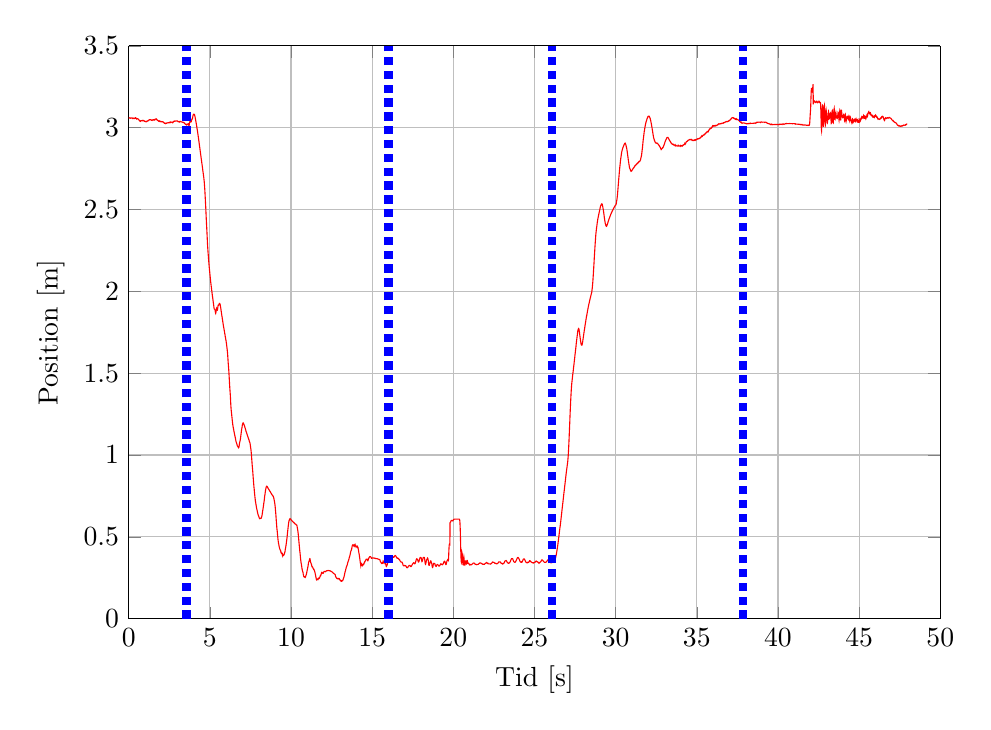
\begin{tikzpicture}

\begin{axis}[%
width=0.85\textwidth,
height=0.6\textwidth,
at={(1.85in,0.746in)},
scale only axis,
separate axis lines,
every outer x axis line/.append style={black},
every x tick label/.append style={font=\color{black}},
xmin=0,
xmax=50,
xlabel={Tid [s]},
xmajorgrids,
every outer y axis line/.append style={black},
every y tick label/.append style={font=\color{black}},
ymin=0,
ymax=3.5,
ylabel={Position [m]},
ymajorgrids,
axis background/.style={fill=white}
]
\addplot [color=red,solid,forget plot]
  table[row sep=crcr]{%
0	3.05864899674712\\
0.00999900999901	3.05964899674712\\
0.01999801999802	3.05964899674712\\
0.02999702999703	3.05864899674712\\
0.03999603999604	3.05864899674712\\
0.04999504999505	3.05864899674712\\
0.05999405999406	3.05964899674712\\
0.06999306999307	3.05864899674712\\
0.07999207999208	3.05864899674712\\
0.08999108999109	3.05799913335067\\
0.0999900999901	3.05864899674712\\
0.10998910998911	3.05799913335067\\
0.11998811998812	3.05864899674712\\
0.12998712998713	3.05864899674712\\
0.13998613998614	3.05864899674712\\
0.14998514998515	3.05799913335067\\
0.15998415998416	3.05799913335067\\
0.16998316998317	3.05864899674712\\
0.17998217998218	3.05799913335067\\
0.18998118998119	3.05799913335067\\
0.1999801999802	3.05864899674712\\
0.20997920997921	3.05864899674712\\
0.21997821997822	3.05799913335067\\
0.22997722997723	3.05864899674712\\
0.23997623997624	3.05799913335067\\
0.24997524997525	3.05634925695508\\
0.25997425997426	3.05734925695508\\
0.26997326997327	3.05734925695508\\
0.27997227997228	3.05634925695508\\
0.28997128997129	3.05734925695508\\
0.2999702999703	3.05799913335067\\
0.30996930996931	3.05699913335067\\
0.31996831996832	3.05634925695508\\
0.32996732996733	3.05734925695508\\
0.33996633996634	3.05669936821023\\
0.34996534996535	3.05604946776602\\
0.35996435996436	3.05604946776602\\
0.36996336996337	3.05604946776602\\
0.37996237996238	3.05634925695508\\
0.38996138996139	3.05864899674712\\
0.3999603999604	3.0599486819432\\
0.40995940995941	3.06059850244313\\
0.41995841995842	3.06059850244313\\
0.42995742995743	3.06059850244313\\
0.43995643995644	3.0599486819432\\
0.44995544995545	3.05764899674712\\
0.45995445995446	3.05569936821023\\
0.46995346995347	3.05539955627235\\
0.47995247995248	3.05474963437911\\
0.48995148995149	3.05309970273625\\
0.4999504999505	3.05409970273625\\
0.50994950994951	3.05474963437911\\
0.51994851994852	3.05439955627235\\
0.52994752994753	3.05539955627235\\
0.53994653994654	3.05539955627235\\
0.54994554994555	3.05474963437911\\
0.55994455994456	3.05409970273625\\
0.56994356994357	3.05344976199368\\
0.57994257994258	3.05279981280135\\
0.58994158994159	3.05114985580921\\
0.5999405999406	3.05149989166721\\
0.60993960993961	3.05019994453351\\
0.61993861993862	3.04889997660004\\
0.62993762993763	3.04659999306667\\
0.63993663993664	3.04629999913333\\
0.64993564993565	3.045\\
0.65993465993466	3.04370000086667\\
0.66993366993367	3.042050002925\\
0.67993267993268	3.04240000693333\\
0.68993168993169	3.04240000693333\\
0.6999306999307	3.04075001354165\\
0.70992970992971	3.04175001354165\\
0.71992871992872	3.04175001354165\\
0.72992772992773	3.04010002339996\\
0.73992673992674	3.04175001354165\\
0.74992574992575	3.04175001354165\\
0.75992475992476	3.04175001354165\\
0.76992376992377	3.04240000693333\\
0.77992277992278	3.04240000693333\\
0.78992178992179	3.04240000693333\\
0.7999207999208	3.043050002925\\
0.80991980991981	3.043050002925\\
0.81991881991882	3.04370000086667\\
0.82991782991783	3.04270000086667\\
0.83991683991684	3.04370000086667\\
0.84991584991585	3.04435000010833\\
0.85991485991486	3.04435000010833\\
0.86991386991387	3.04335000010833\\
0.87991287991288	3.04435000010833\\
0.88991188991189	3.04370000086667\\
0.8999108999109	3.04270000086667\\
0.90990990990991	3.04370000086667\\
0.91990891990892	3.043050002925\\
0.92990792990793	3.043050002925\\
0.93990693990694	3.04240000693333\\
0.94990594990595	3.04175001354165\\
0.95990495990496	3.04110002339996\\
0.96990396990397	3.03945003715824\\
0.97990297990298	3.03980005546649\\
0.98990198990199	3.03980005546649\\
0.999900999901	3.03915007897468\\
1.00990000990001	3.03785014419079\\
1.01989901989902	3.03785014419079\\
1.02989802989803	3.03720018719865\\
1.03989703989704	3.03685014419079\\
1.04989604989605	3.03785014419079\\
1.05989505989506	3.03785014419079\\
1.06989406989407	3.03685014419079\\
1.07989307989308	3.03785014419079\\
1.08989208989209	3.03785014419079\\
1.0998910998911	3.03850010833279\\
1.10989010989011	3.03750010833279\\
1.11988911988912	3.03915007897468\\
1.12988812988813	3.03915007897468\\
1.13988713988714	3.03880005546649\\
1.14988614988615	3.04045003715824\\
1.15988515988516	3.04110002339996\\
1.16988416988417	3.04110002339996\\
1.17988317988318	3.04175001354165\\
1.18988218988219	3.04240000693333\\
1.1998811998812	3.043050002925\\
1.20988020988021	3.04270000086667\\
1.21987921987922	3.04435000010833\\
1.22987822987823	3.045\\
1.23987723987724	3.04629999913333\\
1.24987624987625	3.046949997075\\
1.25987525987526	3.04759999306667\\
1.26987426987427	3.04824998645835\\
1.27987327987328	3.04724998645835\\
1.28987228987229	3.04824998645835\\
1.2998712998713	3.04889997660004\\
1.30987030987031	3.04889997660004\\
1.31986931986932	3.04889997660004\\
1.32986832986833	3.04889997660004\\
1.33986733986734	3.04889997660004\\
1.34986634986635	3.04789997660004\\
1.35986535986536	3.04824998645835\\
1.36986436986437	3.04759999306667\\
1.37986337986338	3.046949997075\\
1.38986238986239	3.04529999913333\\
1.3998613998614	3.04564999989167\\
1.40986040986041	3.04464999989167\\
1.41985941985942	3.04464999989167\\
1.42985842985843	3.04564999989167\\
1.43985743985744	3.04629999913333\\
1.44985644985645	3.04529999913333\\
1.45985545985546	3.046949997075\\
1.46985446985447	3.04759999306667\\
1.47985347985348	3.04759999306667\\
1.48985248985249	3.04724998645835\\
1.4998514998515	3.04824998645835\\
1.50985050985051	3.04824998645835\\
1.51984951984952	3.04824998645835\\
1.52984852984853	3.04724998645835\\
1.53984753984754	3.04824998645835\\
1.54984654984655	3.04759999306667\\
1.55984555984556	3.04759999306667\\
1.56984456984457	3.04659999306667\\
1.57984357984358	3.04824998645835\\
1.58984258984259	3.04724998645835\\
1.5998415998416	3.04789997660004\\
1.60984060984061	3.04954996284176\\
1.61983961983962	3.04954996284176\\
1.62983862983863	3.04919994453351\\
1.63983763983764	3.05149989166721\\
1.64983664983665	3.05214985580921\\
1.65983565983566	3.05279981280135\\
1.66983466983467	3.05279981280135\\
1.67983367983368	3.05279981280135\\
1.68983268983269	3.05344976199368\\
1.6998316998317	3.05179981280135\\
1.70983070983071	3.05214985580921\\
1.71982971982972	3.05084992102532\\
1.72982872982873	3.04854996284176\\
1.73982773982774	3.04889997660004\\
1.74982674982675	3.04759999306667\\
1.75982575982576	3.04629999913333\\
1.76982476982477	3.04435000010833\\
1.77982377982378	3.04435000010833\\
1.78982278982279	3.04370000086667\\
1.7998217998218	3.043050002925\\
1.80982080982081	3.04240000693333\\
1.81981981981982	3.04175001354165\\
1.82981882981883	3.04110002339996\\
1.83981783981784	3.04010002339996\\
1.84981684981685	3.04110002339996\\
1.85981585981586	3.04045003715824\\
1.86981486981487	3.04045003715824\\
1.87981387981388	3.03945003715824\\
1.88981288981289	3.04110002339996\\
1.8998118998119	3.04045003715824\\
1.90981090981091	3.03945003715824\\
1.91980991980992	3.03980005546649\\
1.92980892980893	3.03980005546649\\
1.93980793980794	3.03815007897468\\
1.94980694980695	3.03850010833279\\
1.95980595980596	3.03850010833279\\
1.96980496980497	3.03785014419079\\
1.97980397980398	3.03685014419079\\
1.98980298980299	3.03785014419079\\
1.999801999802	3.03720018719865\\
2.00980100980101	3.03720018719865\\
2.01980001980002	3.03720018719865\\
2.02979902979903	3.03720018719865\\
2.03979803979804	3.03720018719865\\
2.04979704979705	3.03555023800632\\
2.05979605979606	3.03655023800632\\
2.06979506979507	3.03655023800632\\
2.07979407979408	3.03655023800632\\
2.08979308979309	3.03590029726375\\
2.0997920997921	3.03590029726375\\
2.10979110979111	3.03590029726375\\
2.11979011979012	3.03525036562089\\
2.12978912978913	3.03395053223398\\
2.13978813978814	3.03265074304492\\
2.14978714978715	3.03135100325288\\
2.15978615978616	3.03070115350542\\
2.16978516978517	3.02940149755687\\
2.17978417978418	3.02810190400231\\
2.18978318978319	3.02710190400231\\
2.1997821997822	3.02810190400231\\
2.20978120978121	3.02810190400231\\
2.21978021978022	3.02745213224728\\
2.22977922977923	3.02680237804011\\
2.23977823977824	3.02680237804011\\
2.24977724977725	3.02680237804011\\
2.25977625977626	3.02515264203057\\
2.26977526977527	3.02615264203057\\
2.27977427977428	3.02680237804011\\
2.28977328977329	3.02580237804011\\
2.2997722997723	3.02680237804011\\
2.30977130977131	3.02680237804011\\
2.31977031977032	3.02680237804011\\
2.32976932976933	3.02645213224728\\
2.33976833976834	3.02810190400231\\
2.34976734976735	3.02810190400231\\
2.35976635976636	3.02810190400231\\
2.36976536976537	3.02875169265544\\
2.37976437976438	3.02940149755687\\
2.38976338976339	3.02940149755687\\
2.3997623997624	3.02940149755687\\
2.40976140976141	3.0300513180568\\
2.41976041976042	3.0300513180568\\
2.42975942975943	3.03070115350542\\
2.43975843975844	3.03070115350542\\
2.44975744975745	3.03070115350542\\
2.45975645975646	3.0300513180568\\
2.46975546975547	3.03070115350542\\
2.47975447975448	3.03070115350542\\
2.48975348975349	3.03135100325288\\
2.4997524997525	3.03035100325288\\
2.50975150975151	3.03135100325288\\
2.51975051975052	3.03265074304492\\
2.52974952974953	3.03265074304492\\
2.53974853974854	3.03165074304492\\
2.54974754974755	3.03330063178977\\
2.55974655974656	3.03330063178977\\
2.56974556974557	3.03295053223398\\
2.57974457974458	3.03460044372765\\
2.58974358974359	3.03460044372765\\
2.5997425997426	3.03295053223398\\
2.60974160974161	3.03395053223398\\
2.61974061974062	3.03395053223398\\
2.62973962973963	3.03395053223398\\
2.63973863973864	3.03395053223398\\
2.64973764973765	3.03330063178977\\
2.65973665973666	3.03265074304492\\
2.66973566973567	3.03165074304492\\
2.67973467973468	3.03265074304492\\
2.68973368973369	3.03165074304492\\
2.6997326997327	3.03265074304492\\
2.70973170973171	3.03165074304492\\
2.71973071973072	3.03395053223398\\
2.72972972972973	3.03460044372765\\
2.73972873972874	3.03360044372765\\
2.74972774972775	3.03590029726375\\
2.75972675972676	3.03655023800632\\
2.76972576972577	3.03720018719865\\
2.77972477972478	3.03850010833279\\
2.78972378972379	3.03915007897468\\
2.7997227997228	3.03980005546649\\
2.80972180972181	3.03945003715824\\
2.81972081972082	3.04045003715824\\
2.82971982971983	3.04110002339996\\
2.83971883971884	3.04110002339996\\
2.84971784971785	3.03945003715824\\
2.85971685971686	3.03980005546649\\
2.86971586971587	3.03980005546649\\
2.87971487971488	3.03980005546649\\
2.88971388971389	3.03980005546649\\
2.8997128997129	3.04045003715824\\
2.90971190971191	3.04045003715824\\
2.91971091971092	3.04045003715824\\
2.92970992970993	3.04045003715824\\
2.93970893970894	3.04110002339996\\
2.94970794970795	3.04110002339996\\
2.95970695970696	3.04175001354165\\
2.96970596970597	3.04175001354165\\
2.97970497970498	3.04175001354165\\
2.98970398970399	3.04175001354165\\
2.999702999703	3.04175001354165\\
3.00970200970201	3.04110002339996\\
3.01970101970102	3.03880005546649\\
3.02970002970003	3.03850010833279\\
3.03969903969904	3.03785014419079\\
3.04969804969805	3.03620018719865\\
3.05969705969706	3.03655023800632\\
3.06969606969607	3.03590029726375\\
3.07969507969508	3.03590029726375\\
3.08969408969409	3.03590029726375\\
3.0996930996931	3.03590029726375\\
3.10969210969211	3.03590029726375\\
3.11969111969112	3.03590029726375\\
3.12969012969013	3.03490029726375\\
3.13968913968914	3.03720018719865\\
3.14968814968815	3.03685014419079\\
3.15968715968716	3.03785014419079\\
3.16968616968617	3.03785014419079\\
3.17968517968518	3.03785014419079\\
3.18968418968419	3.03785014419079\\
3.1996831996832	3.03785014419079\\
3.20968220968221	3.03720018719865\\
3.21968121968122	3.03655023800632\\
3.22968022968023	3.03490029726375\\
3.23967923967924	3.03525036562089\\
3.24967824967825	3.03525036562089\\
3.25967725967726	3.03525036562089\\
3.26967626967627	3.03525036562089\\
3.27967527967528	3.03525036562089\\
3.28967428967429	3.03460044372765\\
3.2996732996733	3.03360044372765\\
3.30967230967231	3.03395053223398\\
3.31967131967132	3.03395053223398\\
3.32967032967033	3.03395053223398\\
3.33966933966934	3.03295053223398\\
3.34966834966835	3.03330063178977\\
3.35966735966736	3.03265074304492\\
3.36966636966637	3.03200086664933\\
3.37966537966538	3.03135100325288\\
3.38966438966439	3.03070115350542\\
3.3996633996634	3.02940149755687\\
3.40966240966241	3.02840149755687\\
3.41966141966142	3.02940149755687\\
3.42966042966043	3.02875169265544\\
3.43965943965944	3.02810190400231\\
3.44965844965845	3.02680237804011\\
3.45965745965746	3.02485322720326\\
3.46965646965647	3.02355389296302\\
3.47965547965548	3.02225464450718\\
3.48965448965449	3.02095548703273\\
3.4996534996535	3.02030594403749\\
3.50965250965251	3.0196564257363\\
3.51965151965152	3.01900693277869\\
3.52965052965053	3.01835746581414\\
3.53964953964954	3.01835746581414\\
3.54964854964855	3.01770802549212\\
3.55964755964756	3.01640922737341\\
3.56964656964657	3.01640922737341\\
3.57964557964558	3.01770802549212\\
3.58964458964459	3.02095548703273\\
3.5996435996436	3.02195548703273\\
3.60964260964261	3.0206564257363\\
3.61964161964162	3.02100693277869\\
3.62964062964063	3.02035746581414\\
3.63963963963964	3.02040922737341\\
3.64963864963865	3.01911054361776\\
3.65963765963766	3.01946124624945\\
3.66963666963667	3.02111054361776\\
3.67963567963568	3.01816274377835\\
3.68963468963469	3.01656612607659\\
3.6996336996337	3.01461902208376\\
3.70963270963271	3.01332113357835\\
3.71963171963172	3.01232113357835\\
3.72963072963073	3.01721523047403\\
3.73962973962974	3.02435746581414\\
3.74962874962875	3.03050292486838\\
3.75962775962776	3.03535100325288\\
3.76962676962677	3.03660044372765\\
3.77962577962578	3.03755023800632\\
3.78962478962479	3.03820018719865\\
3.7996237996238	3.03620018719865\\
3.80962280962281	3.03620018719865\\
3.81962181962182	3.03385014419079\\
3.82962082962083	3.03380005546649\\
3.83961983961984	3.03540000693333\\
3.84961884961885	3.03629999913333\\
3.85961785961786	3.04014985580921\\
3.86961686961687	3.04364899674712\\
3.87961587961588	3.04814677279674\\
3.88961488961489	3.0503435742637\\
3.8996138996139	3.05288945638224\\
3.90961290961291	3.05278476952597\\
3.91961191961192	3.05532775448052\\
3.92961092961093	3.05716594440794\\
3.93960993960994	3.06094455107996\\
3.94960894960895	3.06765715961246\\
3.95960795960796	3.0730636107665\\
3.96960696960697	3.0768129347378\\
3.97960597960598	3.0792621927028\\
3.98960498960499	3.08041556317588\\
3.999603999604	3.08056321108343\\
4.00960300960301	3.08206244971145\\
4.01960201960202	3.0819150848936\\
4.02960102960103	3.08204614462291\\
4.03960003960004	3.08088991944819\\
4.04959904959905	3.08045020674248\\
4.05959805959806	3.07736922272679\\
4.06959706959707	3.07364798593638\\
4.07959607959608	3.06828719138887\\
4.08959508959509	3.06492627855418\\
4.0995940995941	3.05892627855418\\
4.10959310959311	3.05356524679323\\
4.11959211959212	3.04856524679323\\
4.12959112959113	3.04256524679323\\
4.13959013959014	3.03756524679323\\
4.14958914958915	3.03156524679323\\
4.15958815958816	3.02656524679323\\
4.16958716958717	3.02056524679323\\
4.17958617958618	3.01456524679323\\
4.18958518958519	3.00856524679323\\
4.1995841995842	3.00056524679323\\
4.20958320958321	2.99456524679323\\
4.21958221958222	2.98856524679323\\
4.22958122958123	2.98256524679323\\
4.23958023958024	2.97656524679323\\
4.24957924957925	2.96956524679323\\
4.25957825957826	2.96356524679323\\
4.26957726957727	2.95556524679323\\
4.27957627957628	2.94956524679323\\
4.28957528957529	2.94256524679323\\
4.2995742995743	2.93556524679323\\
4.30957330957331	2.92856524679323\\
4.31957231957232	2.92056524679323\\
4.32957132957133	2.91456524679323\\
4.33957033957034	2.90556524679323\\
4.34956934956935	2.89756524679323\\
4.35956835956836	2.88956524679323\\
4.36956736956737	2.88256524679323\\
4.37956637956638	2.87656524679323\\
4.38956538956539	2.86956524679323\\
4.3995643995644	2.86156524679323\\
4.40956340956341	2.85456524679323\\
4.41956241956242	2.84656524679323\\
4.42956142956143	2.83856524679323\\
4.43956043956044	2.83156524679323\\
4.44955944955945	2.82456524679323\\
4.45955845955846	2.81656524679323\\
4.46955746955747	2.80956524679323\\
4.47955647955648	2.80256524679323\\
4.48955548955549	2.79656524679323\\
4.4995544995545	2.78856524679323\\
4.50955350955351	2.78056524679323\\
4.51955251955252	2.77456524679323\\
4.52955152955153	2.76656524679323\\
4.53955053955054	2.75956524679323\\
4.54954954954955	2.75256524679323\\
4.55954855954856	2.74356524679323\\
4.56954756954757	2.73656524679323\\
4.57954657954658	2.72856524679323\\
4.58954558954559	2.72156524679323\\
4.5995445995446	2.71456524679323\\
4.60954360954361	2.70656524679323\\
4.61954261954262	2.69956524679323\\
4.62954162954163	2.69192627855418\\
4.63954063954064	2.68164798593638\\
4.64953964953965	2.67345020674248\\
4.65953865953866	2.66160910190101\\
4.66953766953767	2.6474814586088\\
4.67953667953668	2.63341999338271\\
4.68953568953569	2.61905933887698\\
4.6995346995347	2.6017485585158\\
4.70953370953371	2.5827710457345\\
4.71953271953272	2.56312620244688\\
4.72953172953173	2.54411123608007\\
4.73953073953074	2.52543387392341\\
4.74952974952975	2.50509574231277\\
4.75952875952876	2.48279981280135\\
4.76952776952777	2.46180005546649\\
4.77952677952678	2.43945213224728\\
4.78952578952579	2.42075987087552\\
4.7995247995248	2.40107708304981\\
4.80952380952381	2.38270339589342\\
4.81952281952282	2.36240191351548\\
4.82952182952183	2.3414778712542\\
4.83952083952084	2.32094066112302\\
4.84951984951985	2.29972676742713\\
4.85951885951886	2.28146983929291\\
4.86951786951787	2.26579590453297\\
4.87951687951688	2.25141413436962\\
4.88951588951589	2.23704502268734\\
4.8995148995149	2.22432417160449\\
4.90951390951391	2.21061455318792\\
4.91951291951292	2.19754914060315\\
4.92951192951193	2.18449329282236\\
4.93951093951094	2.17107752652887\\
4.94950994950995	2.1609281628011\\
4.95950895950896	2.14878285086082\\
4.96950796950797	2.1388976412701\\
4.97950697950698	2.12801393559948\\
4.98950598950599	2.12038637084434\\
4.999504999505	2.10950469677001\\
5.00950400950401	2.09899820186174\\
5.01950301950302	2.08849449097853\\
5.02950202950203	2.07924369206661\\
5.03950103950104	2.06899360417969\\
5.04950004950005	2.05974423231812\\
5.05949905949906	2.05074423231812\\
5.06949806949807	2.04211981645866\\
5.07949707949708	2.03411981645866\\
5.08949608949609	2.02611981645866\\
5.0994950994951	2.01911981645866\\
5.10949410949411	2.00949558147937\\
5.11949311949312	2.00349558147937\\
5.12949212949213	1.99449558147937\\
5.13949113949114	1.98549558147937\\
5.14949014949015	1.97749558147937\\
5.15948915948916	1.96949558147937\\
5.16948816948817	1.96449558147937\\
5.17948717948718	1.95749558147937\\
5.18948618948619	1.94849558147937\\
5.1994851994852	1.94149558147937\\
5.20948420948421	1.93349558147937\\
5.21948321948322	1.92649558147937\\
5.22948222948223	1.91949558147937\\
5.23948123948124	1.91149558147937\\
5.24948024948025	1.90349558147937\\
5.25947925947926	1.89711981645866\\
5.26947826947827	1.89299360417969\\
5.27947727947728	1.89099820186174\\
5.28947628947629	1.89026957144018\\
5.2994752994753	1.88955771392169\\
5.30947430947431	1.88786200049728\\
5.31947331947332	1.8862842693074\\
5.32947232947233	1.88018180074354\\
5.33947133947134	1.87381460970213\\
5.34947034947035	1.86771392315817\\
5.35946935946936	1.86515074499744\\
5.36946836946837	1.86831780175509\\
5.37946737946738	1.87435201406362\\
5.38946638946639	1.88272676742713\\
5.3994653994654	1.89051629784522\\
5.40946440946441	1.89541465254412\\
5.41946341946342	1.89775506422506\\
5.42946242946243	1.89493160306326\\
5.43946143946144	1.89016888058969\\
5.44946044946045	1.88505544892004\\
5.45945945945946	1.8845371492306\\
5.46945846945847	1.88791705611303\\
5.47945747945748	1.89355389296302\\
5.48945648945649	1.90185014419079\\
5.4994554994555	1.90979981280135\\
5.50945450945451	1.91579645031508\\
5.51945351945352	1.91588945638224\\
5.52945252945253	1.91702994068391\\
5.53945153945154	1.91716594440794\\
5.54945054945055	1.91629660410658\\
5.55944955944956	1.91771567782639\\
5.56944856944857	1.92041736295918\\
5.57944757944758	1.9247485585158\\
5.58944658944659	1.92412774417086\\
5.5994455994456	1.92584919029395\\
5.60944460944461	1.92527323257287\\
5.61944361944362	1.92240513358592\\
5.62944262944263	1.91988991944819\\
5.63944163944164	1.91645020674248\\
5.64944064944065	1.90936922272679\\
5.65943965943966	1.90364798593638\\
5.66943866943867	1.89828719138887\\
5.67943767943768	1.89192627855418\\
5.68943668943669	1.88392627855418\\
5.6994356994357	1.87856524679323\\
5.70943470943471	1.87156524679323\\
5.71943371943372	1.86456524679323\\
5.72943272943273	1.85656524679323\\
5.73943173943174	1.85056524679323\\
5.74943074943075	1.84456524679323\\
5.75942975942976	1.83856524679323\\
5.76942876942877	1.83156524679323\\
5.77942777942778	1.82556524679323\\
5.78942678942679	1.81956524679323\\
5.7994257994258	1.81256524679323\\
5.80942480942481	1.80556524679323\\
5.81942381942382	1.79956524679323\\
5.82942282942283	1.79256524679323\\
5.83942183942184	1.78656524679323\\
5.84942084942085	1.77956524679323\\
5.85941985941986	1.77656524679323\\
5.86941886941887	1.77056524679323\\
5.87941787941788	1.76456524679323\\
5.88941688941689	1.75856524679323\\
5.8994158994159	1.75356524679323\\
5.90941490941491	1.74756524679323\\
5.91941391941392	1.74056524679323\\
5.92941292941293	1.73656524679323\\
5.93941193941194	1.72956524679323\\
5.94941094941095	1.72356524679323\\
5.95940995940996	1.71856524679323\\
5.96940896940897	1.71256524679323\\
5.97940797940798	1.70656524679323\\
5.98940698940699	1.70156524679323\\
5.999405999406	1.69556524679323\\
6.00940500940501	1.68864798593638\\
6.01940401940402	1.68345020674248\\
6.02940302940303	1.67488991944819\\
6.03940203940204	1.66668704761376\\
6.04940104940105	1.6584814586088\\
6.05940005940006	1.64927323257287\\
6.06939906939907	1.64170480697775\\
6.07939807939808	1.63184919029395\\
6.08939708939709	1.62105933887698\\
6.0993960993961	1.60832827073079\\
6.10939510939511	1.59364789489834\\
6.11939411939412	1.57795117359601\\
6.12939312939313	1.56324028854519\\
6.13939213939214	1.55016594440794\\
6.14939114939115	1.53738097791624\\
6.15939015939016	1.52588945638224\\
6.16938916938917	1.51144610703698\\
6.17938817938818	1.49474963437911\\
6.18938718938719	1.47740000693333\\
6.1993861993862	1.45940149755687\\
6.20938520938521	1.44040922737341\\
6.21938421938422	1.42472581390473\\
6.22938322938323	1.4083513941634\\
6.23938223938224	1.39428432217361\\
6.24938124938125	1.3802289542655\\
6.25938025938026	1.3671870652622\\
6.26937926937927	1.34994066112302\\
6.27937827937828	1.32844316570074\\
6.28937728937729	1.30827033375155\\
6.2993762993763	1.29305175227443\\
6.30937530937531	1.27913685283811\\
6.31937431937432	1.2687851491584\\
6.32937332937333	1.26098086461437\\
6.33937233937234	1.25154914060315\\
6.34937134937135	1.24112473965414\\
6.35937035937036	1.23170787856209\\
6.36936936936937	1.22255771392169\\
6.37936837936838	1.21315428160874\\
6.38936738936739	1.20313175080229\\
6.3993663993664	1.195372011573\\
6.40936540936541	1.18749449097853\\
6.41936441936442	1.18061855893244\\
6.42936342936343	1.17436882843333\\
6.43936243936244	1.16874423231812\\
6.44936144936145	1.16411981645866\\
6.45936045936046	1.15711981645866\\
6.46935946935947	1.15411981645866\\
6.47935847935848	1.14911981645866\\
6.48935748935749	1.14249558147937\\
6.4993564993565	1.13749558147937\\
6.50935550935551	1.13249558147937\\
6.51935451935452	1.12749558147937\\
6.52935352935353	1.12249558147937\\
6.53935253935254	1.11749558147937\\
6.54935154935155	1.11449558147937\\
6.55935055935056	1.10949558147937\\
6.56934956934957	1.10449558147937\\
6.57934857934858	1.09949558147937\\
6.58934758934759	1.09349558147937\\
6.5993465993466	1.08849558147937\\
6.60934560934561	1.08349558147937\\
6.61934461934462	1.07911981645866\\
6.62934362934363	1.07699360417969\\
6.63934263934264	1.07424369206661\\
6.64934164934165	1.07174599591224\\
6.65934065934066	1.06862456615226\\
6.66933966933967	1.06487781423302\\
6.67933867933868	1.06050469677001\\
6.68933768933769	1.05613175080229\\
6.6993366993367	1.05501393559948\\
6.70933570933571	1.05315428160874\\
6.71933471933472	1.05229877375233\\
6.72933372933373	1.0504473334181\\
6.73933273933274	1.04959988189222\\
6.74933174933175	1.04838809431182\\
6.75933075933076	1.0462842693074\\
6.76932976932977	1.04381460970213\\
6.77932877932878	1.0448823628575\\
6.78932778932779	1.04786541286088\\
6.7993267993268	1.05341413436962\\
6.80932580932581	1.05927033375155\\
6.81932481932482	1.06744316570074\\
6.82932382932383	1.07472314637981\\
6.83932283932284	1.07844894621905\\
6.84932184932185	1.08089657052184\\
6.85932085932086	1.08629021148977\\
6.86931986931987	1.09034284038754\\
6.87931887931888	1.09605544892004\\
6.88931788931789	1.10277974475739\\
6.8993168993169	1.11011054361776\\
6.90931590931591	1.11910190400231\\
6.91931491931492	1.12680005546649\\
6.92931392931393	1.13484992102532\\
6.93931293931294	1.14254786775272\\
6.94931194931195	1.14959077262659\\
6.95931095931096	1.15697660421164\\
6.96930996930997	1.16140786771938\\
6.97930897930898	1.16777365859962\\
6.98930798930799	1.17412465973877\\
6.999306999307	1.18145822133708\\
7.00930600930601	1.18583957265499\\
7.01930501930502	1.19056321108343\\
7.02930402930403	1.19298922175368\\
7.03930303930304	1.19476401514381\\
7.04930204930205	1.19624956629938\\
7.05930105930106	1.19481030499431\\
7.06930006930007	1.19336922272679\\
7.07929907929908	1.19164798593638\\
7.08929808929809	1.18828719138887\\
7.0992970992971	1.18792627855418\\
7.10929610929611	1.18492627855418\\
7.11929511929512	1.18092627855418\\
7.12929412929413	1.17956524679323\\
7.13929313929314	1.17656524679323\\
7.14929214929215	1.17256524679323\\
7.15929115929116	1.16856524679323\\
7.16929016929017	1.16656524679323\\
7.17928917928918	1.16256524679323\\
7.18928818928819	1.15956524679323\\
7.1992871992872	1.15456524679323\\
7.20928620928621	1.15156524679323\\
7.21928521928522	1.14956524679323\\
7.22928422928423	1.14256524679323\\
7.23928323928324	1.14256524679323\\
7.24928224928225	1.13956524679323\\
7.25928125928126	1.13756524679323\\
7.26928026928027	1.13356524679323\\
7.27927927927928	1.12956524679323\\
7.28927828927829	1.12756524679323\\
7.2992772992773	1.12356524679323\\
7.30927630927631	1.12156524679323\\
7.31927531927532	1.11856524679323\\
7.32927432927433	1.11556524679323\\
7.33927333927334	1.11256524679323\\
7.34927234927235	1.10956524679323\\
7.35927135927136	1.10656524679323\\
7.36927036927037	1.10356524679323\\
7.37926937926938	1.10056524679323\\
7.38926838926839	1.09856524679323\\
7.3992673992674	1.09456524679323\\
7.40926640926641	1.09256524679323\\
7.41926541926542	1.08856524679323\\
7.42926442926443	1.08456524679323\\
7.43926343926344	1.08256524679323\\
7.44926244926245	1.07956524679323\\
7.45926145926146	1.07656524679323\\
7.46926046926047	1.07356524679323\\
7.47925947925948	1.06964798593638\\
7.48925848925849	1.06181030499431\\
7.4992574992575	1.05432784191757\\
7.50925650925651	1.04684002179845\\
7.51925551925552	1.04098922175368\\
7.52925452925453	1.03413478610784\\
7.53925353925354	1.02527685362019\\
7.54925254925255	1.01448370215478\\
7.55925155925156	1.00374855851581\\
7.56925056925057	0.990417362959179\\
7.57924957924958	0.976421056978707\\
7.58924858924859	0.964111236080069\\
7.5992475992476	0.948731978767594\\
7.60924660924661	0.936291974507881\\
7.61924561924562	0.926847357969433\\
7.62924462924463	0.914099702736247\\
7.63924363924364	0.903\\
7.64924264924265	0.889900297263754\\
7.65924165924166	0.876853227203262\\
7.66924066924067	0.862162743778347\\
7.67923967923968	0.849779744757391\\
7.68923868923869	0.837407553891201\\
7.6992376992377	0.825342840387538\\
7.70923670923671	0.813644104455836\\
7.71923571923572	0.801606392195098\\
7.72923472923473	0.792872255829136\\
7.73923373923374	0.78115080970605\\
7.74923274923275	0.77044316570074\\
7.75923175923176	0.759750433700624\\
7.76923076923077	0.750712808611128\\
7.77922977922978	0.741327365291011\\
7.78922878922879	0.73295438913047\\
7.7992277992278	0.7232298967563\\
7.80922680922681	0.716785149158399\\
7.81922581922582	0.710614553187919\\
7.82922482922483	0.704814609702128\\
7.83922383922384	0.699020000874383\\
7.84922284922285	0.692230863310192\\
7.85922185922186	0.687707878562093\\
7.86922086922087	0.680557713921694\\
7.87921987921988	0.676040484387654\\
7.88921888921889	0.670525878202367\\
7.8992178992179	0.666641669340668\\
7.90921690921691	0.663013935599477\\
7.91921591921592	0.65787781423302\\
7.92921492921493	0.652372011573004\\
7.93921393921394	0.647869002957078\\
7.94921294921295	0.644618558932439\\
7.95921195921196	0.640368828433326\\
7.96921096921097	0.635744232318117\\
7.97920997920998	0.63311981645866\\
7.98920898920899	0.63111981645866\\
7.999207999208	0.62811981645866\\
8.00920700920701	0.625495581479372\\
8.01920601920602	0.622495581479372\\
8.02920502920503	0.619495581479372\\
8.03920403920404	0.617495581479372\\
8.04920304920305	0.614495581479372\\
8.05920205920206	0.61211981645866\\
8.06920106920107	0.612618558932439\\
8.07920007920008	0.611494490978527\\
8.08919908919909	0.61199820186174\\
8.0991980991981	0.611504696770012\\
8.10919710919711	0.612013935599477\\
8.11919611919612	0.613154281608742\\
8.12919512919513	0.61329877375233\\
8.13919413919414	0.613817299859987\\
8.14919314919315	0.613338388887428\\
8.15919215919216	0.613862000497284\\
8.16919116919117	0.614652059416929\\
8.17919017919018	0.617713923158171\\
8.18918918918919	0.620785149158399\\
8.1991881991882	0.62477277543933\\
8.20918720918721	0.629776643050664\\
8.21918621918622	0.634434753206773\\
8.22918522918523	0.641390898098992\\
8.23918423918424	0.648010778246316\\
8.24918324918325	0.655366465348316\\
8.25918225918226	0.661093334304796\\
8.26918126918127	0.666477871254196\\
8.27918027918028	0.67416831598018\\
8.28917928917929	0.680873797553124\\
8.2991782991783	0.687943887248614\\
8.30917730917731	0.694023395788361\\
8.31917631917632	0.702759870875521\\
8.32917532917533	0.709853227203262\\
8.33917433917434	0.715300631789765\\
8.34917334917335	0.722400006933328\\
8.35917235917236	0.731449761993678\\
8.36917136917137	0.740796450315082\\
8.37917037917038	0.749188020580112\\
8.38916938916939	0.755625414966158\\
8.3991683991684	0.762056112751386\\
8.40916740916741	0.769773658599618\\
8.41916641916642	0.77683168401982\\
8.42916542916543	0.783231016665397\\
8.43916443916444	0.789972994575997\\
8.44916344916345	0.79405933887698\\
8.45916245916246	0.79884919029395\\
8.46916146916147	0.802631277978911\\
8.47916047916048	0.804764015143813\\
8.48915948915949	0.808249566299376\\
8.4991584991585	0.808450206742481\\
8.50915750915751	0.809369222726786\\
8.51915651915652	0.808647985936378\\
8.52915552915553	0.806287191388872\\
8.53915453915454	0.805926278554184\\
8.54915354915355	0.803926278554184\\
8.55915255915256	0.800926278554184\\
8.56915156915157	0.800565246793227\\
8.57915057915058	0.799565246793227\\
8.58914958914959	0.796565246793227\\
8.5991485991486	0.794565246793227\\
8.60914760914761	0.793565246793227\\
8.61914661914662	0.790565246793227\\
8.62914562914563	0.789565246793227\\
8.63914463914464	0.788565246793227\\
8.64914364914365	0.787565246793227\\
8.65914265914266	0.785565246793227\\
8.66914166914167	0.783565246793227\\
8.67914067914068	0.782565246793227\\
8.68913968913969	0.779565246793227\\
8.6991386991387	0.778565246793227\\
8.70913770913771	0.777565246793227\\
8.71913671913672	0.776565246793227\\
8.72913572913573	0.773565246793227\\
8.73913473913474	0.772565246793227\\
8.74913374913375	0.770565246793227\\
8.75913275913276	0.768565246793227\\
8.76913176913177	0.766565246793227\\
8.77913077913078	0.765565246793227\\
8.78912978912979	0.763565246793227\\
8.7991287991288	0.761565246793227\\
8.80912780912781	0.760565246793227\\
8.81912681912682	0.759565246793227\\
8.82912582912583	0.757565246793227\\
8.83912483912484	0.755565246793227\\
8.84912384912385	0.754565246793227\\
8.85912285912286	0.752565246793227\\
8.86912186912187	0.751565246793227\\
8.87912087912088	0.750565246793227\\
8.88911988911989	0.749565246793227\\
8.8991188991189	0.748565246793227\\
8.90911790911791	0.746565246793227\\
8.91911691911692	0.743287191388872\\
8.92911592911593	0.740369222726786\\
8.93911493911494	0.735810304994307\\
8.94911394911395	0.732609101901008\\
8.95911295911296	0.726122789937696\\
8.96911196911197	0.721273232572869\\
8.97911097911098	0.716419993382714\\
8.98910998910999	0.709276853620186\\
8.999108999109	0.703771698059215\\
9.00910800910801	0.697617635448213\\
9.01910701910702	0.688876610643903\\
9.02910602910603	0.67883168401982\\
9.03910503910504	0.666478689167935\\
9.04910404910405	0.65575957527951\\
9.05910305910306	0.643380977916241\\
9.06910206910207	0.632993067221312\\
9.07910107910108	0.617648996747122\\
9.08910008910009	0.603649999891667\\
9.0990990990991	0.590300631789765\\
9.10909810909811	0.577605054072485\\
9.11909711909712	0.563917056113029\\
9.12909612909613	0.552537149230604\\
9.13909513909514	0.543111922258696\\
9.14909414909415	0.535989940188561\\
9.15909315909316	0.523936389233495\\
9.16909216909217	0.513251441484195\\
9.17909117909118	0.503584436824124\\
9.18909018909019	0.492937550288549\\
9.1990891990892	0.482953855377092\\
9.20908820908821	0.47427033375155\\
9.21908721908722	0.469880082290853\\
9.22908622908623	0.460139278955057\\
9.23908523908524	0.457681346061894\\
9.24908424908425	0.4532298967563\\
9.25908325908326	0.444785149158399\\
9.26908226908227	0.441614553187919\\
9.27908127908128	0.436713923158171\\
9.28908028908029	0.433549140603146\\
9.2990792990793	0.429020000874383\\
9.30907830907831	0.426124739654135\\
9.31907731907732	0.423862000497284\\
9.32907632907633	0.419599881892224\\
9.33907533907534	0.418969056874361\\
9.34907434907435	0.417338388887428\\
9.35907335907336	0.415077526528866\\
9.36907236907237	0.4114473334181\\
9.37907137907138	0.40518742648456\\
9.38907038907039	0.4059281628011\\
9.3990693990694	0.402669547404773\\
9.40906840906841	0.400411585330038\\
9.41906741906742	0.398782850860822\\
9.42906642906643	0.397782850860822\\
9.43906543906544	0.397411585330038\\
9.44906444906445	0.394411585330038\\
9.45906345906346	0.393411585330038\\
9.46906246906247	0.387411585330038\\
9.47906147906148	0.391040484387654\\
9.48906048906049	0.385669547404773\\
9.4990594990595	0.3869281628011\\
9.50905850905851	0.386557713921694\\
9.51905751905752	0.38618742648456\\
9.52905652905653	0.387817299859987\\
9.53905553905554	0.388707878562093\\
9.54905454905455	0.387599881892224\\
9.55905355905356	0.390124739654135\\
9.56905256905257	0.391916629913596\\
9.57905157905158	0.394080671542472\\
9.58905058905059	0.396248386146908\\
9.5990495990496	0.398689206392005\\
9.60904860904861	0.402136852838115\\
9.61904761904762	0.40686493498321\\
9.62904662904663	0.409603476997968\\
9.63904563904564	0.41727033375155\\
9.64904464904465	0.423312952386242\\
9.65904365904366	0.429010778246316\\
9.66904266904267	0.435079920688158\\
9.67904167904168	0.440160427345006\\
9.68904068904069	0.445896570521844\\
9.6990396990397	0.454290211489775\\
9.70903870903871	0.459695802243669\\
9.71903771903772	0.468111922258696\\
9.72903672903673	0.474537149230604\\
9.73903573903574	0.483619022083759\\
9.74903474903475	0.491357465814137\\
9.75903375903376	0.49910190400231\\
9.76903276903277	0.50915007897468\\
9.77903177903178	0.51984992102532\\
9.78903078903079	0.52989809599769\\
9.7990297990298	0.538291974507881\\
9.80902880902881	0.547678866421648\\
9.81902781902782	0.557056112751386\\
9.82902682902683	0.565421056978707\\
9.83902583902584	0.573124659738774\\
9.84902484902485	0.580522128745804\\
9.85902385902386	0.588551053780948\\
9.86902286902287	0.593990123049654\\
9.87902187902188	0.598134786107839\\
9.88902088902089	0.600273232572869\\
9.8990198990199	0.604405133585923\\
9.90901890901891	0.608249566299376\\
9.91901791901792	0.608450206742481\\
9.92901692901693	0.609369222726786\\
9.93901593901594	0.610647985936378\\
9.94901494901495	0.609287191388872\\
9.95901395901396	0.608926278554183\\
9.96901296901297	0.608926278554183\\
9.97901197901198	0.606926278554183\\
9.98901098901099	0.605926278554183\\
9.99900999901	0.605565246793227\\
10.009009009009	0.602565246793227\\
10.019008019008	0.601565246793227\\
10.029007029007	0.600565246793227\\
10.039006039006	0.600565246793227\\
10.049005049005	0.599565246793227\\
10.0590040590041	0.598565246793227\\
10.0690030690031	0.596565246793227\\
10.0790020790021	0.595565246793227\\
10.0890010890011	0.594565246793227\\
10.0990000990001	0.594565246793227\\
10.1089991089991	0.593565246793227\\
10.1189981189981	0.591565246793227\\
10.1289971289971	0.590565246793227\\
10.1389961389961	0.589565246793227\\
10.1489951489951	0.588565246793227\\
10.1589941589942	0.588565246793227\\
10.1689931689932	0.587565246793227\\
10.1789921789922	0.585565246793227\\
10.1889911889912	0.585565246793227\\
10.1989901989902	0.584565246793227\\
10.2089892089892	0.583565246793227\\
10.2189882189882	0.582565246793227\\
10.2289872289872	0.580565246793227\\
10.2389862389862	0.579565246793227\\
10.2489852489853	0.579565246793227\\
10.2589842589843	0.578565246793227\\
10.2689832689833	0.577565246793227\\
10.2789822789823	0.577565246793227\\
10.2889812889813	0.577565246793227\\
10.2989802989803	0.576565246793227\\
10.3089793089793	0.574565246793227\\
10.3189783189783	0.573565246793227\\
10.3289773289773	0.572565246793227\\
10.3389763389763	0.572565246793227\\
10.3489753489753	0.572565246793227\\
10.3589743589744	0.570287191388872\\
10.3689733689734	0.567089994040458\\
10.3789723789724	0.559609101901008\\
10.3889713889714	0.555122789937696\\
10.3989703989704	0.549631277978911\\
10.4089694089694	0.544492036446909\\
10.4189684189684	0.53705933887698\\
10.4289674289674	0.529972994575997\\
10.4389664389664	0.522231016665397\\
10.4489654489654	0.511538440974219\\
10.4589644589645	0.500535813049342\\
10.4689634689635	0.49016594440794\\
10.4789624789625	0.479784769525973\\
10.4889614889615	0.468745355492819\\
10.4989604989605	0.457699368210235\\
10.5089595089595	0.446649999891667\\
10.5189585189585	0.435600443727654\\
10.5289575289575	0.425853227203262\\
10.5389565389565	0.415461246249447\\
10.5489555489555	0.406374585033842\\
10.5589545589546	0.397943887248614\\
10.5689535689536	0.388226341400382\\
10.5789525789526	0.376521794381603\\
10.5889515889516	0.367477871254196\\
10.5989505989506	0.357448946219052\\
10.6089496089496	0.350366465348316\\
10.6189486189486	0.341937550288549\\
10.6289476289476	0.33644316570074\\
10.6389466389466	0.331953855377092\\
10.6489456489456	0.323829710564163\\
10.6589446589447	0.317712808611128\\
10.6689436689437	0.311603476997968\\
10.6789426789427	0.303776643050664\\
10.6889416889417	0.29986493498321\\
10.6989406989407	0.295591107551451\\
10.7089397089397	0.291681346061894\\
10.7189387189387	0.288045022687343\\
10.7289377289377	0.286317801755088\\
10.7389367389367	0.281681346061894\\
10.7489357489357	0.274408832267758\\
10.7589347589348	0.26977277543933\\
10.7689337689338	0.268136852838115\\
10.7789327789328	0.259136852838115\\
10.7889317889318	0.25777277543933\\
10.7989307989308	0.255681346061894\\
10.8089298089298	0.255227956381314\\
10.8189288189288	0.255689496127471\\
10.8289278289278	0.256157176063246\\
10.8389268389268	0.256352014063622\\
10.8489258489258	0.253910005959542\\
10.8589248589249	0.252469839292912\\
10.8689238689239	0.251672158082431\\
10.8789228789229	0.253159978201548\\
10.8889218889219	0.253937550288549\\
10.8989208989209	0.257009876950345\\
10.9089199089199	0.260448946219052\\
10.9189189189189	0.263541778662916\\
10.9289179289179	0.265644104455836\\
10.9389169389169	0.268755064225058\\
10.9489159489159	0.272521310832065\\
10.958914958915	0.276943887248614\\
10.968913968914	0.282023395788361\\
10.978912978913	0.288110543617757\\
10.988911988912	0.292904257687232\\
10.998910998911	0.296701153505418\\
11.00891000891	0.301850144190794\\
11.018909018909	0.305649999891667\\
11.028908028908	0.311749634379113\\
11.038907038907	0.316547867752722\\
11.048906048906	0.321993067221312\\
11.0589050589051	0.328082943886971\\
11.0689040689041	0.337111236080069\\
11.0789030789031	0.341888077741304\\
11.0889020889021	0.345362899000361\\
11.0989010989011	0.347891720820438\\
11.1089001089001	0.350124659738774\\
11.1188991188991	0.353001931222212\\
11.1288981288981	0.356522128745804\\
11.1388971388971	0.361038576700398\\
11.1488961488961	0.363906665695204\\
11.1588951588952	0.366483702154776\\
11.1688941688942	0.365839572654994\\
11.1788931788932	0.360683464557324\\
11.1888921888922	0.354231016665397\\
11.1988911988912	0.349063610766505\\
11.2088902088902	0.343891720820438\\
11.2188892188892	0.341010059811439\\
11.2288882288882	0.339421056978707\\
11.2388872388872	0.33683111941031\\
11.2488862488862	0.333944551079962\\
11.2588852588853	0.33240786771938\\
11.2688842688843	0.327220255242609\\
11.2788832788833	0.322380977916241\\
11.2888822888823	0.318837256221653\\
11.2988812988813	0.316590772626588\\
11.3088803088803	0.317291974507881\\
11.3188793188793	0.316993067221312\\
11.3288783288783	0.315044512967267\\
11.3388773388773	0.312796450315082\\
11.3488763488763	0.311197621959888\\
11.3588753588754	0.307948681943196\\
11.3688743688744	0.305699368210235\\
11.3788733788734	0.303749634379113\\
11.3888723888724	0.301799812801348\\
11.3988713988714	0.302499891667208\\
11.4088704088704	0.300549962841758\\
11.4188694188694	0.298599993066672\\
11.4288684288684	0.297649999891667\\
11.4388674388674	0.295050002924999\\
11.4488664488664	0.291800055466489\\
11.4588654588655	0.287900297263753\\
11.4688644688645	0.284650743044921\\
11.4788634788635	0.280751692655437\\
11.4888624888625	0.275553892963022\\
11.4988614988615	0.271006932778688\\
11.5088605088605	0.267110543617757\\
11.5188595188595	0.261917056113029\\
11.5288585288585	0.256725813904735\\
11.5388575388575	0.251537149230604\\
11.5488565488565	0.246351394163404\\
11.5588555588556	0.24181650617843\\
11.5688545688546	0.238578943021293\\
11.5788535788536	0.237284322173611\\
11.5888525888526	0.239521310832065\\
11.5988515988516	0.242055448920038\\
11.6088506088506	0.242703395893421\\
11.6188496188496	0.242351394163404\\
11.6288486288486	0.241351394163404\\
11.6388476388476	0.239703395893421\\
11.6488466488466	0.238703395893421\\
11.6588456588457	0.238295690272717\\
11.6688446688447	0.242185580004124\\
11.6788436788437	0.243428393117799\\
11.6888426888427	0.246672245519481\\
11.6988416988417	0.245970059316087\\
11.7088407088407	0.244619022083759\\
11.7188397188397	0.245268021232406\\
11.7288387288387	0.245566126076593\\
11.7388377388377	0.246864368656229\\
11.7488367488367	0.247811979419888\\
11.7588357588358	0.249058612462073\\
11.7688347688348	0.251305944037491\\
11.7788337788338	0.254203549684918\\
11.7888327888328	0.25810190400231\\
11.7988317988318	0.261650743044921\\
11.8088308088308	0.264250365620887\\
11.8188298188298	0.264900297263753\\
11.8288288288288	0.264200187198652\\
11.8388278388278	0.26815007897468\\
11.8488268488268	0.26875001354165\\
11.8588258588259	0.272\\
11.8688248688249	0.275899976600042\\
11.8788238788239	0.279799812801348\\
11.8888228888229	0.282399556272346\\
11.8988218988219	0.283699368210235\\
11.9088209088209	0.283049467766024\\
11.9188199188199	0.282399556272346\\
11.9288189288189	0.280449761993678\\
11.9388179388179	0.278499891667208\\
11.9488169488169	0.277199944533511\\
11.958815958816	0.277199944533511\\
11.968814968815	0.276549962841758\\
11.978813978814	0.276549962841758\\
11.988812988813	0.278499891667208\\
11.998811998812	0.281099702736247\\
12.008811008811	0.283699368210235\\
12.01881001881	0.285648996747122\\
12.028809028809	0.28759850244313\\
12.038808038808	0.288248307344563\\
12.048807048807	0.288248307344563\\
12.0588060588061	0.288248307344563\\
12.0688050688051	0.288248307344563\\
12.0788040788041	0.288248307344563\\
12.0888030888031	0.288248307344563\\
12.0988020988021	0.288248307344563\\
12.1088011088011	0.287248307344563\\
12.1188001188001	0.28889809599769\\
12.1287991287991	0.28889809599769\\
12.1387981387981	0.289547867752722\\
12.1487971487971	0.290197621959888\\
12.1587961587962	0.290847357969433\\
12.1687951687952	0.290847357969433\\
12.1787941787942	0.291497075131622\\
12.1887931887932	0.292146772796738\\
12.1987921987922	0.292796450315082\\
12.2087912087912	0.292796450315082\\
12.2187902187902	0.292796450315082\\
12.2287892287892	0.293446107036978\\
12.2387882387882	0.293446107036978\\
12.2487872487872	0.293446107036978\\
12.2587862587863	0.293446107036978\\
12.2687852687853	0.294095742312768\\
12.2787842787843	0.294095742312768\\
12.2887832887833	0.294095742312768\\
12.2987822987823	0.294095742312768\\
12.3087813087813	0.294095742312768\\
12.3187803187803	0.293446107036978\\
12.3287793287793	0.293446107036978\\
12.3387783387783	0.293446107036978\\
12.3487773487773	0.293446107036978\\
12.3587763587764	0.293446107036978\\
12.3687753687754	0.292796450315082\\
12.3787743787744	0.292796450315082\\
12.3887733887734	0.292796450315082\\
12.3987723987724	0.292146772796738\\
12.4087714087714	0.292146772796738\\
12.4187704187704	0.291497075131622\\
12.4287694287694	0.291497075131622\\
12.4387684387684	0.290847357969433\\
12.4487674487674	0.290197621959888\\
12.4587664587665	0.289547867752722\\
12.4687654687655	0.28889809599769\\
12.4787644787645	0.288248307344563\\
12.4887634887635	0.288248307344563\\
12.4987624987625	0.28759850244313\\
12.5087615087615	0.286948681943196\\
12.5187605187605	0.286298846494582\\
12.5287595287595	0.284999133350667\\
12.5387585387585	0.284349256955079\\
12.5487575487575	0.283049467766024\\
12.5587565587566	0.282399556272346\\
12.5687555687556	0.281749634379113\\
12.5787545787546	0.281099702736247\\
12.5887535887536	0.279799812801348\\
12.5987525987526	0.279149855809206\\
12.6087516087516	0.27784992102532\\
12.6187506187506	0.277199944533511\\
12.6287496287496	0.276549962841758\\
12.6387486387486	0.275899976600042\\
12.6487476487476	0.27524998645835\\
12.6587466587467	0.274599993066672\\
12.6687456687457	0.273299999133334\\
12.6787446787447	0.272649999891667\\
12.6887436887437	0.272\\
12.6987426987427	0.271350000108333\\
12.7087417087417	0.270700000866667\\
12.7187407187407	0.269400006933328\\
12.7287397287397	0.265500108332792\\
12.7387387387387	0.260950532233976\\
12.7487377487377	0.25640149755687\\
12.7587367587368	0.255802378040112\\
12.7687357687358	0.253853227203262\\
12.7787347787348	0.252254644507181\\
12.7887337887338	0.250305944037491\\
12.7987327987328	0.249357465814137\\
12.8087318087318	0.247409227373412\\
12.8187308187308	0.246461246249447\\
12.8287298287298	0.246513539974059\\
12.8387288387288	0.245566126076593\\
12.8487278487278	0.244268021232406\\
12.8587268587269	0.244619022083759\\
12.8687258687259	0.243970059316087\\
12.8787248787249	0.244970059316087\\
12.8887238887239	0.244672245519481\\
12.8987228987229	0.245374585033842\\
12.9087219087219	0.244428393117799\\
12.9187209187209	0.244131138617235\\
12.9287199287199	0.24283405559206\\
12.9387189387189	0.242537149230604\\
12.9487179487179	0.245537149230604\\
12.958716958717	0.245537149230604\\
12.968715968716	0.24459213228062\\
12.978714978715	0.242999443081989\\
12.988713988714	0.240111922258696\\
12.998712998713	0.238873797553125\\
13.008712008712	0.236637100999639\\
13.018711018711	0.236048826403993\\
13.02871002871	0.234755064225058\\
13.038709038709	0.234461559025781\\
13.048708048708	0.234521794381603\\
13.0587070587071	0.232582637040821\\
13.0687060687061	0.232644104455836\\
13.0787050787051	0.231060396338976\\
13.0887040887041	0.228477871254196\\
13.0987030987031	0.228541778662916\\
13.1087021087021	0.228251441484195\\
13.1187011187011	0.228606392195098\\
13.1287001287001	0.230251441484195\\
13.1386991386991	0.231251441484195\\
13.1486981486981	0.232606392195098\\
13.1586971586972	0.231961423299602\\
13.1686961686962	0.232671729269208\\
13.1786951786952	0.232027005424003\\
13.1886941886942	0.233671729269208\\
13.1986931986932	0.234961423299602\\
13.2086922086922	0.239541778662916\\
13.2186912186912	0.242477871254196\\
13.2286902286902	0.245414652544119\\
13.2386892386892	0.248352105101665\\
13.2486882486882	0.251290211489774\\
13.2586872586873	0.253875340261226\\
13.2686862686863	0.255814904410435\\
13.2786852786853	0.261048826403993\\
13.2886842886843	0.265284322173611\\
13.2986832986833	0.27081650617843\\
13.3086823086823	0.275703395893421\\
13.3186813186813	0.278943887248614\\
13.3286803286803	0.28483405559206\\
13.3386793386793	0.288428393117799\\
13.3486783486783	0.291023395788361\\
13.3586773586774	0.294619022083759\\
13.3686763686764	0.299513539974059\\
13.3786753786754	0.303759870875521\\
13.3886743886744	0.306357465814137\\
13.3986733986734	0.311605054072485\\
13.4086724086724	0.315203549684918\\
13.4186714186714	0.318152642030567\\
13.4286704286704	0.319452132247278\\
13.4386694386694	0.321751692655437\\
13.4486684486684	0.325051318056804\\
13.4586674586675	0.327000866649334\\
13.4686664686665	0.330600443727654\\
13.4786654786655	0.334850144190794\\
13.4886644886645	0.33975001354165\\
13.4986634986635	0.343\\
13.5086625086625	0.346599993066672\\
13.5186615186615	0.348549962841758\\
13.5286605286605	0.35184992102532\\
13.5386595386595	0.354799812801348\\
13.5486585486585	0.357099702736247\\
13.5586575586576	0.360699368210235\\
13.5686565686566	0.363948681943196\\
13.5786555786556	0.368847357969433\\
13.5886545886546	0.373446107036978\\
13.5986535986536	0.374745355492819\\
13.6086526086526	0.379993067221312\\
13.6186516186516	0.381941387537927\\
13.6286506286506	0.386240129124479\\
13.6386496386496	0.388837256221653\\
13.6486486486486	0.394380977916241\\
13.6586476586477	0.400571606882201\\
13.6686466686467	0.404462850769396\\
13.6786456786457	0.409000556918011\\
13.6886446886447	0.413888077741304\\
13.6986436986437	0.415478689167935\\
13.7086427086427	0.417773658599618\\
13.7186417186417	0.418715677826389\\
13.7286407286407	0.422951173596007\\
13.7386397386397	0.427478205618397\\
13.7486387486387	0.43329378592657\\
13.7586377586378	0.438103429478156\\
13.7686367686368	0.443906665695204\\
13.7786357786358	0.447127744170864\\
13.7886347886348	0.448703024518754\\
13.7986337986338	0.449990123049655\\
13.8086328086328	0.450920079311842\\
13.8186318186318	0.450206248291809\\
13.8286308286308	0.45084919029395\\
13.8386298386298	0.450206248291809\\
13.8486288486288	0.448276853620186\\
13.8586278586279	0.44634661945751\\
13.8686268686269	0.444415563175876\\
13.8786258786259	0.443127744170864\\
13.8886248886249	0.446127744170864\\
13.8986238986239	0.442483702154776\\
13.9086229086229	0.443839572654994\\
13.9186219186219	0.443839572654994\\
13.9286209286209	0.444839572654994\\
13.9386199386199	0.446839572654994\\
13.9486189486189	0.449551053780948\\
13.958617958618	0.444262192702802\\
13.968616968617	0.443972994575997\\
13.978615978616	0.443328270730792\\
13.988614988615	0.442748558515805\\
13.998613998614	0.440167570325583\\
14.008613008613	0.443876610643903\\
14.018612018612	0.442585347455881\\
14.028611028611	0.441647894898335\\
14.03861003861	0.439709788510226\\
14.048609048609	0.439063610766505\\
14.0586080586081	0.439417362959179\\
14.0686070686071	0.442124659738774\\
14.0786060786061	0.442185095589565\\
14.0886050886051	0.442598086484515\\
14.0986040986041	0.435362899000361\\
14.1086031086031	0.435478689167935\\
14.1186021186021	0.432888077741304\\
14.1286011286011	0.433648605836596\\
14.1386001386001	0.42675957527951\\
14.1485991485991	0.42392291695019\\
14.1585981585982	0.417433873923407\\
14.1685971685972	0.410291974507881\\
14.1785961785962	0.403146772796738\\
14.1885951885952	0.399349256955079\\
14.1985941985942	0.39424998645835\\
14.2085932085932	0.387450037158242\\
14.2185922185922	0.378650743044921\\
14.2285912285912	0.372853227203262\\
14.2385902385902	0.365708025492119\\
14.2485892485892	0.357917056113029\\
14.2585882585883	0.351428393117799\\
14.2685872685873	0.342647542001126\\
14.2785862785863	0.33881650617843\\
14.2885852885853	0.332284322173611\\
14.2985842985843	0.325048826403993\\
14.3085833085833	0.330048826403993\\
14.3185823185823	0.330226341400382\\
14.3285813285813	0.333407553891201\\
14.3385803385803	0.335999443081989\\
14.3485793485793	0.334351394163404\\
14.3585783585784	0.329407553891201\\
14.3685773685774	0.326464186950658\\
14.3785763785764	0.32481650617843\\
14.3885753885754	0.325111922258696\\
14.3985743985744	0.324055448920038\\
14.4085734085734	0.326943887248614\\
14.4185724185724	0.329131138617235\\
14.4285714285714	0.330725813904735\\
14.4385704385704	0.329374585033842\\
14.4485694485694	0.329672245519481\\
14.4585684585685	0.329619022083759\\
14.4685674685675	0.329566126076593\\
14.4785664785665	0.331811979419888\\
14.4885654885655	0.334357465814137\\
14.4985644985645	0.337904257687232\\
14.5085635085635	0.34210190400231\\
14.5185625185625	0.344351003252878\\
14.5285615285615	0.346300631789765\\
14.5385605385605	0.345250365620887\\
14.5485595485595	0.348500108332792\\
14.5585585585586	0.350100023399958\\
14.5685575685576	0.351050002924999\\
14.5785565785566	0.353299999133333\\
14.5885555885556	0.356549962841758\\
14.5985545985546	0.357149855809206\\
14.6085536085536	0.358099702736247\\
14.6185526185526	0.360699368210235\\
14.6285516285516	0.362648996747122\\
14.6385506385506	0.362298846494582\\
14.6485496485496	0.362948681943196\\
14.6585486585487	0.36359850244313\\
14.6685476685477	0.36389809599769\\
14.6785466785467	0.36389809599769\\
14.6885456885457	0.361948681943196\\
14.6985446985447	0.359999133350666\\
14.7085437085437	0.357399556272346\\
14.7185427185427	0.354799812801348\\
14.7285417285417	0.35284992102532\\
14.7385407385407	0.35284992102532\\
14.7485397485397	0.356749634379113\\
14.7585387585388	0.361298846494582\\
14.7685377685378	0.365197621959888\\
14.7785367785368	0.367796450315082\\
14.7885357885358	0.370095742312768\\
14.7985347985348	0.370394945927515\\
14.8085338085338	0.371694055962509\\
14.8185328185328	0.373642534185863\\
14.8285318285318	0.375590772626588\\
14.8385308385308	0.377538753750553\\
14.8485298485298	0.378837256221653\\
14.8585288585289	0.378837256221653\\
14.8685278685279	0.378837256221653\\
14.8785268785269	0.379486460025941\\
14.8885258885259	0.379486460025941\\
14.8985248985249	0.378837256221653\\
14.9085239085239	0.378188020580112\\
14.9185229185229	0.376889456382243\\
14.9285219285219	0.374291974507881\\
14.9385209385209	0.371694055962509\\
14.9485199485199	0.369745355492819\\
14.958518958519	0.369095742312768\\
14.968517968518	0.369095742312768\\
14.978516978517	0.369745355492819\\
14.988515988516	0.370394945927515\\
14.998514998515	0.371044512967267\\
15.008514008514	0.371044512967267\\
15.018513018513	0.371044512967267\\
15.028512028512	0.370394945927515\\
15.038511038511	0.370394945927515\\
15.04851004851	0.369745355492819\\
15.0585090585091	0.369745355492819\\
15.0685080685081	0.370394945927515\\
15.0785070785071	0.371044512967267\\
15.0885060885061	0.371044512967267\\
15.0985050985051	0.371694055962509\\
15.1085041085041	0.371694055962509\\
15.1185031185031	0.371044512967267\\
15.1285021285021	0.370394945927515\\
15.1385011385011	0.369745355492819\\
15.1485001485001	0.369745355492819\\
15.1584991584992	0.369095742312768\\
15.1684981684982	0.369095742312768\\
15.1784971784972	0.369095742312768\\
15.1884961884962	0.368446107036978\\
15.1984951984952	0.367796450315082\\
15.2084942084942	0.367796450315082\\
15.2184932184932	0.367796450315082\\
15.2284922284922	0.367146772796738\\
15.2384912384912	0.367146772796738\\
15.2484902484902	0.367146772796738\\
15.2584892584893	0.367146772796738\\
15.2684882684883	0.367146772796738\\
15.2784872784873	0.367146772796738\\
15.2884862884863	0.366497075131622\\
15.2984852984853	0.366497075131622\\
15.3084843084843	0.365847357969433\\
15.3184833184833	0.365847357969433\\
15.3284823284823	0.365197621959888\\
15.3384813384813	0.365197621959888\\
15.3484803484803	0.365197621959888\\
15.3584793584794	0.364547867752722\\
15.3684783684784	0.36389809599769\\
15.3784773784774	0.36389809599769\\
15.3884763884764	0.363248307344563\\
15.3984753984754	0.36259850244313\\
15.4084744084744	0.36259850244313\\
15.4184734184734	0.361948681943196\\
15.4284724284724	0.361298846494582\\
15.4384714384714	0.361298846494582\\
15.4484704484704	0.361298846494582\\
15.4584694584695	0.361298846494582\\
15.4684684684685	0.360648996747122\\
15.4784674784675	0.359349256955079\\
15.4884664884665	0.354799812801348\\
15.4984654984655	0.351899976600042\\
15.5084645084645	0.348\\
15.5184635184635	0.346050002924999\\
15.5284625284625	0.345100023399958\\
15.5384615384615	0.34415007897468\\
15.5484605484605	0.342200187198652\\
15.5584595584596	0.342600443727654\\
15.5684585684586	0.339000866649333\\
15.5784575784576	0.33740149755687\\
15.5884565884566	0.33710190400231\\
15.5984555984556	0.336452132247278\\
15.6084546084546	0.336802378040112\\
15.6184536184536	0.338802378040112\\
15.6284526284526	0.34010190400231\\
15.6384516384516	0.34240149755687\\
15.6484506484506	0.34340149755687\\
15.6584496584497	0.34210190400231\\
15.6684486684487	0.34710190400231\\
15.6784476784477	0.343751692655437\\
15.6884466884467	0.34440149755687\\
15.6984456984457	0.344051318056804\\
15.7084447084447	0.344051318056804\\
15.7184437184437	0.34340149755687\\
15.7284427284427	0.34210190400231\\
15.7384417384417	0.346452132247278\\
15.7484407484407	0.34210190400231\\
15.7584397584398	0.344701153505418\\
15.7684387684388	0.346650743044921\\
15.7784377784378	0.347950532233976\\
15.7884367884368	0.346600443727654\\
15.7984357984358	0.346600443727654\\
15.8084348084348	0.346600443727654\\
15.8184338184338	0.342650743044921\\
15.8284328284328	0.337452132247278\\
15.8384318384318	0.330955487032732\\
15.8484308484308	0.327759870875521\\
15.8584298584299	0.323162743778347\\
15.8684288684289	0.324215230474027\\
15.8784278784279	0.321864368656229\\
15.8884268884269	0.325513539974059\\
15.8984258984259	0.325811979419888\\
15.9084249084249	0.324461246249447\\
15.9184239184239	0.325759870875521\\
15.9284229284229	0.329708025492119\\
15.9384219384219	0.333605054072485\\
15.9484209484209	0.338802378040112\\
15.95841995842	0.343351003252878\\
15.968418968419	0.348900297263753\\
15.978417978418	0.352800055466489\\
15.988416988417	0.357350000108333\\
15.998415998416	0.361899976600042\\
16.008415008415	0.365799812801348\\
16.018414018414	0.368399556272346\\
16.028413028413	0.369049467766024\\
16.038412038412	0.370349256955079\\
16.048411048411	0.372298846494582\\
16.0584100584101	0.374248307344563\\
16.0684090684091	0.375547867752722\\
16.0784080784081	0.375547867752722\\
16.0884070884071	0.37489809599769\\
16.0984060984061	0.372298846494582\\
16.1084051084051	0.370349256955079\\
16.1184041184041	0.369049467766024\\
16.1284031284031	0.368399556272346\\
16.1384021384021	0.368399556272346\\
16.1484011484011	0.368399556272346\\
16.1584001584002	0.369049467766024\\
16.1683991683992	0.370999133350666\\
16.1783981783982	0.372298846494582\\
16.1883971883972	0.372948681943196\\
16.1983961983962	0.37359850244313\\
16.2083952083952	0.375547867752722\\
16.2183942183942	0.376847357969433\\
16.2283932283932	0.377497075131622\\
16.2383922383922	0.378796450315082\\
16.2483912483912	0.378796450315082\\
16.2583902583903	0.378146772796738\\
16.2683892683893	0.377497075131622\\
16.2783882783883	0.378146772796738\\
16.2883872883873	0.377497075131622\\
16.2983862983863	0.375547867752722\\
16.3083853083853	0.374248307344563\\
16.3183843183843	0.374248307344563\\
16.3283833283833	0.37489809599769\\
16.3383823383823	0.375547867752722\\
16.3483813483813	0.376847357969433\\
16.3583803583804	0.378146772796738\\
16.3683793683794	0.380095742312768\\
16.3783783783784	0.382044512967267\\
16.3883773883774	0.383343574263697\\
16.3983763983764	0.383993067221312\\
16.4083754083754	0.385291974507881\\
16.4183744183744	0.385941387537927\\
16.4283734283734	0.385291974507881\\
16.4383724383724	0.385291974507881\\
16.4483714483714	0.383993067221312\\
16.4583704583705	0.382694055962509\\
16.4683694683695	0.380745355492819\\
16.4783684783685	0.378796450315082\\
16.4883674883675	0.376847357969433\\
16.4983664983665	0.37489809599769\\
16.5083655083655	0.372298846494582\\
16.5183645183645	0.370999133350666\\
16.5283635283635	0.370349256955079\\
16.5383625383625	0.370349256955079\\
16.5483615483615	0.369699368210235\\
16.5583605583606	0.370349256955079\\
16.5683595683596	0.370349256955079\\
16.5783585783586	0.369699368210235\\
16.5883575883576	0.369049467766024\\
16.5983565983566	0.369049467766024\\
16.6083556083556	0.368399556272346\\
16.6183546183546	0.367749634379113\\
16.6283536283536	0.365799812801348\\
16.6383526383526	0.36384992102532\\
16.6483516483517	0.363199944533511\\
16.6583506583507	0.362549962841758\\
16.6683496683497	0.36124998645835\\
16.6783486783487	0.361599993066672\\
16.6883476883477	0.359299999133333\\
16.6983466983467	0.357350000108333\\
16.7083457083457	0.355400006933328\\
16.7183447183447	0.352800055466489\\
16.7283437283437	0.351500108332792\\
16.7383427383427	0.350200187198652\\
16.7483417483417	0.348900297263753\\
16.7583407583408	0.347600443727654\\
16.7683397683398	0.346950532233976\\
16.7783387783388	0.346950532233976\\
16.7883377883378	0.346300631789765\\
16.7983367983368	0.345650743044921\\
16.8083358083358	0.345650743044921\\
16.8183348183348	0.345650743044921\\
16.8283338283338	0.345650743044921\\
16.8383328383328	0.345000866649333\\
16.8483318483318	0.343701153505418\\
16.8583308583309	0.34110190400231\\
16.8683298683299	0.337853227203262\\
16.8783288783289	0.335904257687232\\
16.8883278883279	0.332656425736303\\
16.8983268983269	0.329409227373412\\
16.9083259083259	0.326811979419888\\
16.9183249183249	0.324864368656229\\
16.9283239283239	0.323566126076593\\
16.9383229383229	0.322917056113029\\
16.9483219483219	0.322268021232406\\
16.958320958321	0.322268021232406\\
16.96831996832	0.322917056113029\\
16.978318978319	0.324215230474027\\
16.988317988318	0.325513539974059\\
16.998316998317	0.325513539974059\\
17.008316008316	0.324864368656229\\
17.018315018315	0.324215230474027\\
17.028314028314	0.323566126076593\\
17.038313038313	0.323566126076593\\
17.048312048312	0.323566126076593\\
17.0583110583111	0.323566126076593\\
17.0683100683101	0.322917056113029\\
17.0783090783091	0.322268021232406\\
17.0883080883081	0.320970059316087\\
17.0983070983071	0.318374585033842\\
17.1083061083061	0.316428393117799\\
17.1183051183051	0.314482575345937\\
17.1283041283041	0.312537149230604\\
17.1383031383031	0.311888763919931\\
17.1483021483021	0.31124042472049\\
17.1583011583012	0.31124042472049\\
17.1683001683002	0.311888763919931\\
17.1782991782992	0.313185580004124\\
17.1882981882982	0.31383405559206\\
17.1982971982972	0.314482575345937\\
17.2082962082962	0.315779744757391\\
17.2182952182952	0.317725813904735\\
17.2282942282942	0.320321133578352\\
17.2382932382932	0.321619022083759\\
17.2482922482922	0.322268021232406\\
17.2582912582913	0.322268021232406\\
17.2682902682903	0.323566126076593\\
17.2782892782893	0.324864368656229\\
17.2882882882883	0.325513539974059\\
17.2982872982873	0.325513539974059\\
17.3082863082863	0.324864368656229\\
17.3182853182853	0.324864368656229\\
17.3282843282843	0.324864368656229\\
17.3382833382833	0.324215230474027\\
17.3482823482823	0.322268021232406\\
17.3582813582814	0.320321133578352\\
17.3682803682804	0.318374585033842\\
17.3782793782794	0.317725813904735\\
17.3882783882784	0.317725813904735\\
17.3982773982774	0.319023395788361\\
17.4082764082764	0.319672245519481\\
17.4182754182754	0.320321133578352\\
17.4282744282744	0.322268021232406\\
17.4382734382734	0.324215230474027\\
17.4482724482724	0.326811979419888\\
17.4582714582715	0.328759870875521\\
17.4682704682705	0.330058612462073\\
17.4782694782695	0.332006932778688\\
17.4882684882685	0.333955487032732\\
17.4982674982675	0.335254644507181\\
17.5082665082665	0.336553892963022\\
17.5182655182655	0.337853227203262\\
17.5282645282645	0.339152642030567\\
17.5382635382635	0.340452132247278\\
17.5482625482625	0.34110190400231\\
17.5582615582616	0.341751692655437\\
17.5682605682606	0.34110190400231\\
17.5782595782596	0.340452132247278\\
17.5882585882586	0.338502924868378\\
17.5982575982576	0.337203549684918\\
17.6082566082566	0.336553892963022\\
17.6182556182556	0.335254644507181\\
17.6282546282546	0.335254644507181\\
17.6382536382536	0.335904257687232\\
17.6482526482526	0.337203549684918\\
17.6582516582517	0.339802378040112\\
17.6682506682507	0.343701153505418\\
17.6782496782497	0.346950532233976\\
17.6882486882487	0.350850144190794\\
17.6982476982477	0.354100023399958\\
17.7082467082467	0.358\\
17.7182457182457	0.36124998645835\\
17.7282447282447	0.363199944533511\\
17.7382437382437	0.365149855809206\\
17.7482427482427	0.365799812801348\\
17.7582417582418	0.365149855809206\\
17.7682407682408	0.364499891667208\\
17.7782397782398	0.36384992102532\\
17.7882387882388	0.362549962841758\\
17.7982377982378	0.359949997075001\\
17.8082368082368	0.357350000108333\\
17.8182358182358	0.354100023399958\\
17.8282348282348	0.351500108332792\\
17.8382338382338	0.348250365620887\\
17.8482328482328	0.345650743044921\\
17.8582318582319	0.345650743044921\\
17.8682308682309	0.346300631789765\\
17.8782298782299	0.348250365620887\\
17.8882288882289	0.351500108332792\\
17.8982278982279	0.356050002924999\\
17.9082269082269	0.360599993066672\\
17.9182259182259	0.364499891667208\\
17.9282249282249	0.367099702736247\\
17.9382239382239	0.369049467766024\\
17.9482229482229	0.371648996747122\\
17.958221958222	0.37359850244313\\
17.968220968221	0.37359850244313\\
17.97821997822	0.37359850244313\\
17.988218988219	0.37359850244313\\
17.998217998218	0.372948681943196\\
18.008217008217	0.372948681943196\\
18.018216018216	0.371648996747122\\
18.028215028215	0.367099702736247\\
18.038214038214	0.361899976600042\\
18.048213048213	0.356050002924999\\
18.0582120582121	0.351500108332792\\
18.0682110682111	0.348900297263753\\
18.0782100782101	0.350200187198652\\
18.0882090882091	0.352800055466489\\
18.0982080982081	0.356050002924999\\
18.1082071082071	0.359949997075001\\
18.1182061182061	0.363199944533511\\
18.1282051282051	0.367099702736247\\
18.1382041382041	0.370999133350666\\
18.1482031482031	0.374248307344563\\
18.1582021582022	0.37489809599769\\
18.1682011682012	0.37489809599769\\
18.1782001782002	0.37489809599769\\
18.1881991881992	0.374248307344563\\
18.1981981981982	0.37489809599769\\
18.2081972081972	0.37489809599769\\
18.2181962181962	0.372948681943196\\
18.2281952281952	0.367749634379113\\
18.2381942381942	0.359299999133333\\
18.2481932481932	0.351500108332792\\
18.2581922581923	0.344351003252878\\
18.2681912681913	0.337203549684918\\
18.2781902781903	0.333305944037491\\
18.2881892881893	0.332006932778688\\
18.2981882981883	0.334605054072485\\
18.3081873081873	0.338502924868378\\
18.3181863181863	0.343051318056804\\
18.3281853281853	0.348250365620887\\
18.3381843381843	0.352800055466489\\
18.3481833481833	0.357350000108333\\
18.3581823581824	0.360599993066672\\
18.3681813681814	0.361899976600042\\
18.3781803781804	0.362549962841758\\
18.3881793881794	0.365149855809206\\
18.3981783981784	0.368399556272346\\
18.4081774081774	0.370999133350666\\
18.4181764181764	0.370349256955079\\
18.4281754281754	0.367749634379113\\
18.4381744381744	0.363199944533511\\
18.4481734481734	0.359299999133333\\
18.4581724581725	0.354100023399958\\
18.4681714681715	0.345650743044921\\
18.4781704781705	0.336553892963022\\
18.4881694881695	0.329409227373412\\
18.4981684981685	0.326162743778347\\
18.5081675081675	0.325513539974059\\
18.5181665181665	0.325513539974059\\
18.5281655281655	0.328110543617757\\
18.5381645381645	0.332006932778688\\
18.5481635481635	0.336553892963022\\
18.5581625581626	0.340452132247278\\
18.5681615681616	0.343051318056804\\
18.5781605781606	0.346300631789765\\
18.5881595881596	0.348900297263753\\
18.5981585981586	0.350850144190794\\
18.6081576081576	0.352800055466489\\
18.6181566181566	0.35215007897468\\
18.6281556281556	0.350200187198652\\
18.6381546381546	0.345650743044921\\
18.6481536481536	0.34240149755687\\
18.6581526581527	0.340452132247278\\
18.6681516681517	0.337853227203262\\
18.6781506781507	0.331357465814137\\
18.6881496881497	0.324215230474027\\
18.6981486981487	0.317725813904735\\
18.7081477081477	0.31383405559206\\
18.7181467181467	0.312537149230604\\
18.7281457281457	0.313185580004124\\
18.7381447381447	0.315779744757391\\
18.7481437481437	0.320970059316087\\
18.7581427581428	0.326162743778347\\
18.7681417681418	0.330708025492119\\
18.7781407781408	0.333955487032732\\
18.7881397881398	0.337553892963022\\
18.7981387981388	0.337203549684918\\
18.8081378081378	0.337853227203262\\
18.8181368181368	0.337853227203262\\
18.8281358281358	0.337853227203262\\
18.8381348381348	0.337203549684918\\
18.8481338481338	0.336553892963022\\
18.8581328581329	0.335904257687232\\
18.8681318681319	0.333955487032732\\
18.8781308781309	0.329409227373412\\
18.8881298881299	0.325513539974059\\
18.8981288981289	0.322917056113029\\
18.9081279081279	0.321619022083759\\
18.9181269181269	0.320970059316087\\
18.9281259281259	0.319672245519481\\
18.9381249381249	0.319023395788361\\
18.9481239481239	0.319672245519481\\
18.958122958123	0.322917056113029\\
18.968121968122	0.325513539974059\\
18.978120978121	0.327461246249447\\
18.98811998812	0.328759870875521\\
18.998118998119	0.329409227373412\\
19.008118008118	0.330058612462073\\
19.018117018117	0.330708025492119\\
19.028116028116	0.330058612462073\\
19.038115038115	0.329409227373412\\
19.048114048114	0.328759870875521\\
19.0581130581131	0.328110543617757\\
19.0681120681121	0.327461246249447\\
19.0781110781111	0.326162743778347\\
19.0881100881101	0.324864368656229\\
19.0981090981091	0.323566126076593\\
19.1081081081081	0.322268021232406\\
19.1181071181071	0.320970059316087\\
19.1281061281061	0.321619022083759\\
19.1381051381051	0.322268021232406\\
19.1481041481041	0.322917056113029\\
19.1581031581032	0.324215230474027\\
19.1681021681022	0.326162743778347\\
19.1781011781012	0.328110543617757\\
19.1881001881002	0.328759870875521\\
19.1980991980992	0.329409227373412\\
19.2080982080982	0.330058612462073\\
19.2180972180972	0.331357465814137\\
19.2280962280962	0.334955487032732\\
19.2380952380952	0.334605054072485\\
19.2480942480942	0.334605054072485\\
19.2580932580933	0.333955487032732\\
19.2680922680923	0.333955487032732\\
19.2780912780913	0.333305944037491\\
19.2880902880903	0.332006932778688\\
19.2980892980893	0.330708025492119\\
19.3080883080883	0.329409227373412\\
19.3180873180873	0.329409227373412\\
19.3280863280863	0.329409227373412\\
19.3380853380853	0.330708025492119\\
19.3480843480843	0.331357465814137\\
19.3580833580834	0.332656425736303\\
19.3680823680824	0.334605054072485\\
19.3780813780814	0.336904257687232\\
19.3880803880804	0.338502924868378\\
19.3980793980794	0.340452132247278\\
19.4080784080784	0.343701153505418\\
19.4180774180774	0.346950532233976\\
19.4280764280764	0.348900297263753\\
19.4380754380754	0.350200187198652\\
19.4480744480744	0.350850144190794\\
19.4580734580735	0.350850144190794\\
19.4680724680725	0.350200187198652\\
19.4780714780715	0.348250365620887\\
19.4880704880705	0.346950532233976\\
19.4980694980695	0.343701153505418\\
19.5080685080685	0.340452132247278\\
19.5180675180675	0.336553892963022\\
19.5280665280665	0.332656425736303\\
19.5380655380655	0.330708025492119\\
19.5480645480645	0.330708025492119\\
19.5580635580636	0.332006932778688\\
19.5680625680626	0.334605054072485\\
19.5780615780616	0.339152642030567\\
19.5880605880606	0.343701153505418\\
19.5980595980596	0.348250365620887\\
19.6080586080586	0.35215007897468\\
19.6180576180576	0.354100023399958\\
19.6280566280566	0.35475001354165\\
19.6380556380556	0.356050002924999\\
19.6480546480546	0.358649999891667\\
19.6580536580537	0.360599993066672\\
19.6680526680527	0.362549962841758\\
19.6780516780517	0.361899976600042\\
19.6880506880507	0.359949997075001\\
19.6980496980497	0.358\\
19.7080487080487	0.370349256955079\\
19.7180477180477	0.395678866421648\\
19.7280467280467	0.420304197756331\\
19.7380457380457	0.439038576700398\\
19.7480447480447	0.450633534651684\\
19.7580437580438	0.456419993382714\\
19.7680427680428	0.457704806977746\\
19.7780417780418	0.455777438633992\\
19.7880407880408	0.454492036446909\\
19.7980397980398	0.587586469973694\\
19.8080388080388	0.588194458732129\\
19.8180378180378	0.588802217296124\\
19.8280368280368	0.589409745057921\\
19.8380358380358	0.591230937456005\\
19.8480348480348	0.594867008649756\\
19.8580338580339	0.597286326853848\\
19.8680328680329	0.598494552656777\\
19.8780318780319	0.599701816481816\\
19.8880308880309	0.599701816481816\\
19.8980298980299	0.599701816481816\\
19.9080289080289	0.599701816481816\\
19.9180279180279	0.600305086143396\\
19.9280269280269	0.599701816481816\\
19.9380259380259	0.599701816481816\\
19.9480249480249	0.599098305118439\\
19.958023958024	0.597890559700582\\
19.968022968023	0.597286326853848\\
19.978021978022	0.597890559700582\\
19.988020988021	0.599701816481816\\
19.99801999802	0.602113438885876\\
20.008019008019	0.603919594609053\\
20.018018018018	0.605723537057539\\
20.028017028017	0.606324356561507\\
20.038016038016	0.606924927741139\\
20.048015048015	0.607525249995864\\
20.0580140580141	0.608125322725359\\
20.0680130680131	0.608125322725359\\
20.0780120780121	0.608125322725359\\
20.0880110880111	0.608125322725359\\
20.0980100980101	0.608125322725359\\
20.1080091080091	0.608125322725359\\
20.1180081180081	0.608125322725359\\
20.1280071280071	0.608125322725359\\
20.1380061380061	0.608125322725359\\
20.1480051480051	0.608125322725359\\
20.1580041580042	0.608125322725359\\
20.1680031680032	0.608125322725359\\
20.1780021780022	0.608125322725359\\
20.1880011880012	0.608125322725359\\
20.1980001980002	0.608125322725359\\
20.2079992079992	0.608125322725359\\
20.2179982179982	0.608125322725359\\
20.2279972279972	0.608125322725359\\
20.2379962379962	0.608125322725359\\
20.2479952479952	0.608125322725359\\
20.2579942579943	0.608125322725359\\
20.2679932679933	0.608125322725359\\
20.2779922779923	0.608125322725359\\
20.2879912879913	0.608125322725359\\
20.2979902979903	0.608125322725359\\
20.3079893079893	0.608125322725359\\
20.3179883179883	0.608125322725359\\
20.3279873279873	0.608125322725359\\
20.3379863379863	0.608125322725359\\
20.3479853479853	0.608125322725359\\
20.3579843579844	0.608125322725359\\
20.3679833679834	0.608125322725359\\
20.3779823779824	0.606924927741139\\
20.3879813879814	0.603919594609053\\
20.3979803979804	0.598494552656777\\
20.4079794079794	0.585761128612787\\
20.4179784179784	0.565550710807051\\
20.4279774279774	0.53888018354134\\
20.4379764379764	0.501751613853092\\
20.4479754479754	0.458347064539243\\
20.4579744579745	0.417715677826389\\
20.4679734679735	0.385941387537927\\
20.4779724779725	0.36384992102532\\
20.4879714879715	0.349550238006322\\
20.4979704979705	0.343051318056804\\
20.5079695079695	0.346300631789765\\
20.5179685179685	0.36384992102532\\
20.5279675279675	0.385291974507881\\
20.5379665379665	0.400220255242609\\
20.5479655479655	0.395678866421648\\
20.5579645579646	0.380745355492819\\
20.5679635679636	0.363199944533511\\
20.5779625779626	0.347600443727654\\
20.5879615879616	0.335904257687232\\
20.5979605979606	0.329409227373412\\
20.6079596079596	0.328759870875521\\
20.6179586179586	0.336553892963022\\
20.6279576279576	0.354100023399958\\
20.6379566379566	0.372948681943196\\
20.6479556479556	0.378146772796738\\
20.6579546579547	0.370349256955079\\
20.6679536679537	0.358\\
20.6779526779527	0.345000866649333\\
20.6879516879517	0.335254644507181\\
20.6979506979507	0.328759870875521\\
20.7079497079497	0.327461246249447\\
20.7179487179487	0.330058612462073\\
20.7279477279477	0.337853227203262\\
20.7379467379467	0.347600443727654\\
20.7479457479457	0.353450037158242\\
20.7579447579448	0.353450037158242\\
20.7679437679438	0.348900297263753\\
20.7779427779428	0.344351003252878\\
20.7879417879418	0.339152642030567\\
20.7979407979408	0.336553892963022\\
20.8079398079398	0.335254644507181\\
20.8179388179388	0.337853227203262\\
20.8279378279378	0.343051318056804\\
20.8379368379368	0.350200187198652\\
20.8479358479358	0.355400006933328\\
20.8579348579349	0.355400006933328\\
20.8679338679339	0.35215007897468\\
20.8779328779329	0.346950532233976\\
20.8879318879319	0.341751692655437\\
20.8979308979309	0.337853227203262\\
20.9079299079299	0.335904257687232\\
20.9179289179289	0.335904257687232\\
20.9279279279279	0.336553892963022\\
20.9379269379269	0.337203549684918\\
20.9479259479259	0.337853227203262\\
20.957924957925	0.336553892963022\\
20.967923967924	0.335254644507181\\
20.977922977923	0.332656425736303\\
20.987921987922	0.330708025492119\\
20.997920997921	0.328759870875521\\
21.00792000792	0.328110543617757\\
21.017919017919	0.328110543617757\\
21.027918027918	0.328759870875521\\
21.037917037917	0.328759870875521\\
21.047916047916	0.330058612462073\\
21.0579150579151	0.330708025492119\\
21.0679140679141	0.330708025492119\\
21.0779130779131	0.330058612462073\\
21.0879120879121	0.329409227373412\\
21.0979110979111	0.329409227373412\\
21.1079101079101	0.329409227373412\\
21.1179091179091	0.330058612462073\\
21.1279081279081	0.330708025492119\\
21.1379071379071	0.332006932778688\\
21.1479061479061	0.332656425736303\\
21.1579051579052	0.333305944037491\\
21.1679041679042	0.333955487032732\\
21.1779031779032	0.334605054072485\\
21.1879021879022	0.335904257687232\\
21.1979011979012	0.337203549684918\\
21.2079002079002	0.337853227203262\\
21.2178992178992	0.338502924868378\\
21.2278982278982	0.339152642030567\\
21.2378972378972	0.339152642030567\\
21.2478962478962	0.339152642030567\\
21.2578952578953	0.339802378040112\\
21.2678942678943	0.339802378040112\\
21.2778932778933	0.339802378040112\\
21.2878922878923	0.339152642030567\\
21.2978912978913	0.338502924868378\\
21.3078903078903	0.337853227203262\\
21.3178893178893	0.336553892963022\\
21.3278883278883	0.333955487032732\\
21.3378873378873	0.332656425736303\\
21.3478863478863	0.333656425736303\\
21.3578853578854	0.332656425736303\\
21.3678843678844	0.332006932778688\\
21.3778833778834	0.332006932778688\\
21.3878823878824	0.332006932778688\\
21.3978813978814	0.331357465814137\\
21.4078804078804	0.331357465814137\\
21.4178794178794	0.330708025492119\\
21.4278784278784	0.330708025492119\\
21.4378774378774	0.330058612462073\\
21.4478764478764	0.329409227373412\\
21.4578754578755	0.330058612462073\\
21.4678744678745	0.330708025492119\\
21.4778734778735	0.331357465814137\\
21.4878724878725	0.332006932778688\\
21.4978714978715	0.332006932778688\\
21.5078705078705	0.331357465814137\\
21.5178695178695	0.331357465814137\\
21.5278685278685	0.331357465814137\\
21.5378675378675	0.332006932778688\\
21.5478665478665	0.333305944037491\\
21.5578655578656	0.334605054072485\\
21.5678645678646	0.335254644507181\\
21.5778635778636	0.335904257687232\\
21.5878625878626	0.337203549684918\\
21.5978615978616	0.337853227203262\\
21.6078606078606	0.338502924868378\\
21.6178596178596	0.338502924868378\\
21.6278586278586	0.339802378040112\\
21.6378576378576	0.339152642030567\\
21.6478566478566	0.339152642030567\\
21.6578556578557	0.339802378040112\\
21.6678546678547	0.340452132247278\\
21.6778536778537	0.340452132247278\\
21.6878526878527	0.340452132247278\\
21.6978516978517	0.339802378040112\\
21.7078507078507	0.339152642030567\\
21.7178497178497	0.337853227203262\\
21.7278487278487	0.336553892963022\\
21.7378477378477	0.335904257687232\\
21.7478467478467	0.335904257687232\\
21.7578457578458	0.335254644507181\\
21.7678447678448	0.335904257687232\\
21.7778437778438	0.335254644507181\\
21.7878427878428	0.334605054072485\\
21.7978417978418	0.333305944037491\\
21.8078408078408	0.332006932778688\\
21.8178398178398	0.332006932778688\\
21.8278388278388	0.332006932778688\\
21.8378378378378	0.332656425736303\\
21.8478368478368	0.332656425736303\\
21.8578358578359	0.333305944037491\\
21.8678348678349	0.333305944037491\\
21.8778338778339	0.332656425736303\\
21.8878328878329	0.332656425736303\\
21.8978318978319	0.332656425736303\\
21.9078309078309	0.332656425736303\\
21.9178299178299	0.332656425736303\\
21.9278289278289	0.333955487032732\\
21.9378279378279	0.334605054072485\\
21.9478269478269	0.335254644507181\\
21.957825957826	0.336553892963022\\
21.967824967825	0.337203549684918\\
21.977823977824	0.337853227203262\\
21.987822987823	0.338502924868378\\
21.997821997822	0.339802378040112\\
22.007821007821	0.340452132247278\\
22.01782001782	0.341751692655437\\
22.027819027819	0.34240149755687\\
22.037818037818	0.343051318056804\\
22.047817047817	0.343701153505418\\
22.0578160578161	0.343051318056804\\
22.0678150678151	0.341751692655437\\
22.0778140778141	0.339152642030567\\
22.0878130878131	0.337853227203262\\
22.0978120978121	0.337203549684918\\
22.1078111078111	0.338502924868378\\
22.1178101178101	0.338502924868378\\
22.1278091278091	0.339152642030567\\
22.1378081378081	0.338502924868378\\
22.1478071478071	0.337203549684918\\
22.1578061578062	0.335904257687232\\
22.1678051678052	0.335254644507181\\
22.1778041778042	0.334605054072485\\
22.1878031878032	0.334605054072485\\
22.1978021978022	0.334605054072485\\
22.2078012078012	0.334605054072485\\
22.2178002178002	0.334605054072485\\
22.2277992277992	0.334605054072485\\
22.2377982377982	0.334605054072485\\
22.2477972477972	0.334605054072485\\
22.2577962577963	0.334605054072485\\
22.2677952677953	0.333955487032732\\
22.2777942777943	0.333955487032732\\
22.2877932877933	0.333955487032732\\
22.2977922977923	0.333305944037491\\
22.3077913077913	0.333955487032732\\
22.3177903177903	0.335254644507181\\
22.3277893277893	0.336553892963022\\
22.3377883377883	0.337203549684918\\
22.3477873477873	0.337853227203262\\
22.3577863577864	0.338502924868378\\
22.3677853677854	0.339152642030567\\
22.3777843777844	0.340452132247278\\
22.3877833877834	0.34240149755687\\
22.3977823977824	0.344351003252878\\
22.4077814077814	0.345650743044921\\
22.4177804177804	0.346300631789765\\
22.4277794277794	0.346300631789765\\
22.4377784377784	0.345650743044921\\
22.4477774477774	0.345000866649333\\
22.4577764577765	0.344351003252878\\
22.4677754677755	0.344351003252878\\
22.4777744777745	0.344351003252878\\
22.4877734877735	0.343701153505418\\
22.4977724977725	0.343701153505418\\
22.5077715077715	0.343701153505418\\
22.5177705177705	0.34240149755687\\
22.5277695277695	0.341751692655437\\
22.5377685377685	0.340452132247278\\
22.5477675477675	0.339152642030567\\
22.5577665577666	0.338502924868378\\
22.5677655677656	0.338502924868378\\
22.5777645777646	0.338502924868378\\
22.5877635877636	0.338502924868378\\
22.5977625977626	0.338502924868378\\
22.6077616077616	0.338502924868378\\
22.6177606177606	0.337853227203262\\
22.6277596277596	0.337203549684918\\
22.6377586377586	0.335904257687232\\
22.6477576477576	0.335254644507181\\
22.6577566577567	0.335254644507181\\
22.6677556677557	0.335254644507181\\
22.6777546777547	0.335254644507181\\
22.6877536877537	0.335904257687232\\
22.6977526977527	0.335904257687232\\
22.7077517077517	0.336553892963022\\
22.7177507177507	0.336553892963022\\
22.7277497277497	0.337203549684918\\
22.7377487377487	0.337853227203262\\
22.7477477477477	0.339152642030567\\
22.7577467577468	0.340452132247278\\
22.7677457677458	0.34240149755687\\
22.7777447777448	0.343701153505418\\
22.7877437877438	0.345650743044921\\
22.7977427977428	0.346950532233976\\
22.8077418077418	0.346950532233976\\
22.8177408177408	0.346950532233976\\
22.8277398277398	0.346950532233976\\
22.8377388377388	0.346950532233976\\
22.8477378477378	0.346300631789765\\
22.8577368577369	0.346300631789765\\
22.8677358677359	0.346950532233976\\
22.8777348777349	0.346950532233976\\
22.8877338877339	0.346950532233976\\
22.8977328977329	0.345650743044921\\
22.9077319077319	0.344351003252878\\
22.9177309177309	0.34240149755687\\
22.9277299277299	0.340452132247278\\
22.9377289377289	0.339152642030567\\
22.9477279477279	0.338502924868378\\
22.957726957727	0.337853227203262\\
22.967725967726	0.338502924868378\\
22.977724977725	0.338502924868378\\
22.987723987724	0.337853227203262\\
22.997722997723	0.337203549684918\\
23.007722007722	0.335904257687232\\
23.017721017721	0.335904257687232\\
23.02772002772	0.335254644507181\\
23.037719037719	0.335254644507181\\
23.047718047718	0.333955487032732\\
23.0577170577171	0.334605054072485\\
23.0677160677161	0.335904257687232\\
23.0777150777151	0.337203549684918\\
23.0877140877141	0.337203549684918\\
23.0977130977131	0.337853227203262\\
23.1077121077121	0.339152642030567\\
23.1177111177111	0.339802378040112\\
23.1277101277101	0.340452132247278\\
23.1377091377091	0.34240149755687\\
23.1477081477081	0.343701153505418\\
23.1577071577072	0.346300631789765\\
23.1677061677062	0.349550238006322\\
23.1777051777052	0.351500108332792\\
23.1877041877042	0.352800055466489\\
23.1977031977032	0.353450037158242\\
23.2077022077022	0.353450037158242\\
23.2177012177012	0.354100023399958\\
23.2277002277002	0.354100023399958\\
23.2376992376992	0.35475001354165\\
23.2476982476982	0.355400006933328\\
23.2576972576973	0.35475001354165\\
23.2676962676963	0.354100023399958\\
23.2776952776953	0.35215007897468\\
23.2876942876943	0.350850144190794\\
23.2976932976933	0.348900297263753\\
23.3076923076923	0.346950532233976\\
23.3176913176913	0.345650743044921\\
23.3276903276903	0.343051318056804\\
23.3376893376893	0.341751692655437\\
23.3476883476883	0.341751692655437\\
23.3576873576874	0.341751692655437\\
23.3676863676864	0.340452132247278\\
23.3776853776854	0.339802378040112\\
23.3876843876844	0.339152642030567\\
23.3976833976834	0.338502924868378\\
23.4076824076824	0.338502924868378\\
23.4176814176814	0.338502924868378\\
23.4276804276804	0.339152642030567\\
23.4376794376794	0.339802378040112\\
23.4476784476784	0.340452132247278\\
23.4576774576775	0.341751692655437\\
23.4676764676765	0.34240149755687\\
23.4776754776755	0.343701153505418\\
23.4876744876745	0.345000866649333\\
23.4976734976735	0.346300631789765\\
23.5076725076725	0.348250365620887\\
23.5176715176715	0.350850144190794\\
23.5276705276705	0.353450037158242\\
23.5376695376695	0.356700000866666\\
23.5476685476685	0.359299999133333\\
23.5576675576676	0.361899976600042\\
23.5676665676666	0.363199944533511\\
23.5776655776656	0.365149855809206\\
23.5876645876646	0.366449761993678\\
23.5976635976636	0.367099702736247\\
23.6076626076626	0.367099702736247\\
23.6176616176616	0.367099702736247\\
23.6276606276606	0.367099702736247\\
23.6376596376596	0.367099702736247\\
23.6476586476586	0.366449761993678\\
23.6576576576577	0.366149855809206\\
23.6676566676567	0.363199944533511\\
23.6776556776557	0.360599993066672\\
23.6876546876547	0.357350000108333\\
23.6976536976537	0.35475001354165\\
23.7076527076527	0.35215007897468\\
23.7176517176517	0.349550238006322\\
23.7276507276507	0.348250365620887\\
23.7376497376497	0.347600443727654\\
23.7476487476487	0.346950532233976\\
23.7576477576478	0.346300631789765\\
23.7676467676468	0.345650743044921\\
23.7776457776458	0.345000866649333\\
23.7876447876448	0.345000866649333\\
23.7976437976438	0.345000866649333\\
23.8076428076428	0.345000866649333\\
23.8176418176418	0.345650743044921\\
23.8276408276408	0.346950532233976\\
23.8376398376398	0.348250365620887\\
23.8476388476388	0.350200187198652\\
23.8576378576379	0.35215007897468\\
23.8676368676369	0.353450037158242\\
23.8776358776359	0.356050002924999\\
23.8876348876349	0.358\\
23.8976338976339	0.360599993066672\\
23.9076329076329	0.363199944533511\\
23.9176319176319	0.365799812801348\\
23.9276309276309	0.368399556272346\\
23.9376299376299	0.370349256955079\\
23.9476289476289	0.372298846494582\\
23.957627957628	0.372948681943196\\
23.967626967627	0.37359850244313\\
23.977625977626	0.374248307344563\\
23.987624987625	0.374248307344563\\
23.997623997624	0.37359850244313\\
24.007623007623	0.372298846494582\\
24.017622017622	0.370999133350666\\
24.027621027621	0.369049467766024\\
24.03762003762	0.367099702736247\\
24.047619047619	0.365799812801348\\
24.0576180576181	0.363199944533511\\
24.0676170676171	0.36124998645835\\
24.0776160776161	0.358649999891667\\
24.0876150876151	0.355400006933328\\
24.0976140976141	0.35215007897468\\
24.1076131076131	0.350200187198652\\
24.1176121176121	0.348900297263753\\
24.1276111276111	0.347600443727654\\
24.1376101376101	0.346300631789765\\
24.1476091476091	0.345650743044921\\
24.1576081576082	0.345000866649333\\
24.1676071676072	0.344351003252878\\
24.1776061776062	0.344351003252878\\
24.1876051876052	0.346000866649333\\
24.1976041976042	0.345000866649333\\
24.2076032076032	0.345650743044921\\
24.2176022176022	0.345000866649333\\
24.2276012276012	0.345000866649333\\
24.2376002376002	0.346300631789765\\
24.2475992475992	0.348250365620887\\
24.2575982575983	0.350850144190794\\
24.2675972675973	0.353450037158242\\
24.2775962775963	0.355400006933328\\
24.2875952875953	0.357350000108333\\
24.2975942975943	0.359949997075001\\
24.3075933075933	0.361899976600042\\
24.3175923175923	0.36384992102532\\
24.3275913275913	0.364499891667208\\
24.3375903375903	0.365149855809206\\
24.3475893475893	0.365149855809206\\
24.3575883575884	0.365149855809206\\
24.3675873675874	0.365149855809206\\
24.3775863775864	0.36384992102532\\
24.3875853875854	0.362549962841758\\
24.3975843975844	0.360599993066672\\
24.4075834075834	0.358649999891667\\
24.4175824175824	0.356050002924999\\
24.4275814275814	0.353450037158242\\
24.4375804375804	0.351500108332792\\
24.4475794475794	0.349550238006322\\
24.4575784575785	0.348250365620887\\
24.4675774675775	0.346300631789765\\
24.4775764775765	0.345000866649333\\
24.4875754875755	0.343701153505418\\
24.4975744975745	0.343051318056804\\
24.5075735075735	0.34240149755687\\
24.5175725175725	0.34240149755687\\
24.5275715275715	0.341751692655437\\
24.5375705375705	0.341751692655437\\
24.5475695475695	0.341751692655437\\
24.5575685575686	0.342751692655437\\
24.5675675675676	0.341751692655437\\
24.5775665775666	0.341751692655437\\
24.5875655875656	0.34240149755687\\
24.5975645975646	0.344051318056804\\
24.6075636075636	0.343701153505418\\
24.6175626175626	0.344351003252878\\
24.6275616275616	0.345000866649333\\
24.6375606375606	0.345650743044921\\
24.6475596475596	0.345000866649333\\
24.6575586575587	0.346950532233976\\
24.6675576675577	0.348250365620887\\
24.6775566775567	0.350200187198652\\
24.6875556875557	0.35215007897468\\
24.6975546975547	0.350850144190794\\
24.7075537075537	0.35215007897468\\
24.7175527175527	0.352800055466489\\
24.7275517275517	0.353450037158242\\
24.7375507375507	0.352800055466489\\
24.7475497475497	0.351500108332792\\
24.7575487575488	0.348900297263753\\
24.7675477675478	0.348250365620887\\
24.7775467775468	0.348250365620887\\
24.7875457875458	0.347600443727654\\
24.7975447975448	0.346950532233976\\
24.8075438075438	0.345650743044921\\
24.8175428175428	0.345000866649333\\
24.8275418275418	0.344351003252878\\
24.8375408375408	0.343701153505418\\
24.8475398475398	0.343051318056804\\
24.8575388575389	0.34240149755687\\
24.8675378675379	0.341751692655437\\
24.8775368775369	0.341751692655437\\
24.8875358875359	0.341751692655437\\
24.8975348975349	0.341751692655437\\
24.9075339075339	0.341751692655437\\
24.9175329175329	0.341751692655437\\
24.9275319275319	0.341751692655437\\
24.9375309375309	0.339802378040112\\
24.9475299475299	0.339802378040112\\
24.957528957529	0.340452132247278\\
24.967527967528	0.341751692655437\\
24.977526977527	0.34240149755687\\
24.987525987526	0.343051318056804\\
24.997524997525	0.344351003252878\\
25.007524007524	0.345000866649333\\
25.017523017523	0.345000866649333\\
25.027522027522	0.345000866649333\\
25.037521037521	0.346300631789765\\
25.04752004752	0.346300631789765\\
25.0575190575191	0.347600443727654\\
25.0675180675181	0.348900297263753\\
25.0775170775171	0.350200187198652\\
25.0875160875161	0.351500108332792\\
25.0975150975151	0.35215007897468\\
25.1075141075141	0.350200187198652\\
25.1175131175131	0.349550238006322\\
25.1275121275121	0.349550238006322\\
25.1375111375111	0.348900297263753\\
25.1475101475101	0.348900297263753\\
25.1575091575092	0.348900297263753\\
25.1675081675082	0.348250365620887\\
25.1775071775072	0.347600443727654\\
25.1875061875062	0.346950532233976\\
25.1975051975052	0.345650743044921\\
25.2075042075042	0.345000866649333\\
25.2175032175032	0.345000866649333\\
25.2275022275022	0.344351003252878\\
25.2375012375012	0.344351003252878\\
25.2475002475002	0.343701153505418\\
25.2574992574993	0.34240149755687\\
25.2674982674983	0.339802378040112\\
25.2774972774973	0.338502924868378\\
25.2874962874963	0.339802378040112\\
25.2974952974953	0.34110190400231\\
25.3074943074943	0.341751692655437\\
25.3174933174933	0.34240149755687\\
25.3274923274923	0.343701153505418\\
25.3374913374913	0.344351003252878\\
25.3474903474903	0.345000866649333\\
25.3574893574894	0.345650743044921\\
25.3674883674884	0.346950532233976\\
25.3774873774874	0.347600443727654\\
25.3874863874864	0.348900297263753\\
25.3974853974854	0.350200187198652\\
25.4074844074844	0.351500108332792\\
25.4174834174834	0.353450037158242\\
25.4274824274824	0.35475001354165\\
25.4374814374814	0.357350000108333\\
25.4474804474804	0.358649999891667\\
25.4574794574795	0.359299999133333\\
25.4674784674785	0.359299999133333\\
25.4774774774775	0.358649999891667\\
25.4874764874765	0.358649999891667\\
25.4974754974755	0.357350000108333\\
25.5074745074745	0.356700000866666\\
25.5174735174735	0.355400006933328\\
25.5274725274725	0.353450037158242\\
25.5374715374715	0.35215007897468\\
25.5474705474705	0.350850144190794\\
25.5574695574696	0.349550238006322\\
25.5674685674686	0.348250365620887\\
25.5774675774676	0.347600443727654\\
25.5874665874666	0.346300631789765\\
25.5974655974656	0.345650743044921\\
25.6074646074646	0.345000866649333\\
25.6174636174636	0.344351003252878\\
25.6274626274626	0.344351003252878\\
25.6374616374616	0.344351003252878\\
25.6474606474606	0.343701153505418\\
25.6574596574597	0.343701153505418\\
25.6674586674587	0.343701153505418\\
25.6774576774577	0.343701153505418\\
25.6874566874567	0.344351003252878\\
25.6974556974557	0.345000866649333\\
25.7074547074547	0.345650743044921\\
25.7174537174537	0.345650743044921\\
25.7274527274527	0.346300631789765\\
25.7374517374517	0.347600443727654\\
25.7474507474507	0.348900297263753\\
25.7574497574498	0.350200187198652\\
25.7674487674488	0.351500108332792\\
25.7774477774478	0.353450037158242\\
25.7874467874468	0.35475001354165\\
25.7974457974458	0.356050002924999\\
25.8074448074448	0.358\\
25.8174438174438	0.359299999133333\\
25.8274428274428	0.359299999133333\\
25.8374418374418	0.359299999133333\\
25.8474408474408	0.358649999891667\\
25.8574398574399	0.358649999891667\\
25.8674388674389	0.357350000108333\\
25.8774378774379	0.356700000866666\\
25.8874368874369	0.355400006933328\\
25.8974358974359	0.353450037158242\\
25.9074349074349	0.35215007897468\\
25.9174339174339	0.350200187198652\\
25.9274329274329	0.348900297263753\\
25.9374319374319	0.348250365620887\\
25.9474309474309	0.346950532233976\\
25.95742995743	0.344351003252878\\
25.967428967429	0.343701153505418\\
25.977427977428	0.343051318056804\\
25.987426987427	0.34240149755687\\
25.997425997426	0.34240149755687\\
26.007425007425	0.341751692655437\\
26.017424017424	0.341751692655437\\
26.027423027423	0.341751692655437\\
26.037422037422	0.341751692655437\\
26.047421047421	0.341751692655437\\
26.0574200574201	0.34240149755687\\
26.0674190674191	0.343051318056804\\
26.0774180774181	0.343051318056804\\
26.0874170874171	0.343701153505418\\
26.0974160974161	0.344351003252878\\
26.1074151074151	0.346000866649333\\
26.1174141174141	0.348650743044921\\
26.1274131274131	0.348950532233976\\
26.1374121374121	0.350600443727654\\
26.1474111474111	0.353900297263753\\
26.1574101574102	0.353900297263753\\
26.1674091674092	0.356900297263753\\
26.1774081774082	0.358600443727654\\
26.1874071874072	0.357000866649334\\
26.1974061974062	0.357051318056804\\
26.2074052074052	0.358452132247278\\
26.2174042174042	0.358203549684918\\
26.2274032274032	0.357955487032733\\
26.2374022374022	0.360357465814137\\
26.2474012474012	0.364110543617757\\
26.2574002574003	0.364215230474027\\
26.2673992673993	0.365321133578352\\
26.2773982773983	0.36607708304981\\
26.2873972873973	0.367482575345937\\
26.2973962973963	0.371185580004124\\
26.3073953073953	0.375537149230604\\
26.3173943173943	0.379888763919931\\
26.3273933273933	0.38424042472049\\
26.3373923373923	0.38924042472049\\
26.3473913473913	0.39424042472049\\
26.3573903573904	0.40024042472049\\
26.3673893673894	0.40559213228062\\
26.3773883773884	0.41159213228062\\
26.3873873873874	0.41759213228062\\
26.3973863973864	0.42459213228062\\
26.4073854073854	0.43159213228062\\
26.4173844173844	0.43759213228062\\
26.4273834273834	0.44459213228062\\
26.4373824373824	0.45159213228062\\
26.4473814473814	0.45959213228062\\
26.4573804573805	0.46659213228062\\
26.4673794673795	0.47359213228062\\
26.4773784773785	0.48259213228062\\
26.4873774873775	0.48959213228062\\
26.4973764973765	0.49859213228062\\
26.5073755073755	0.50559213228062\\
26.5173745173745	0.51524042472049\\
26.5273735273735	0.52259213228062\\
26.5373725373725	0.53159213228062\\
26.5473715473715	0.53959213228062\\
26.5573705573706	0.54659213228062\\
26.5673695673696	0.55659213228062\\
26.5773685773686	0.56159213228062\\
26.5873675873676	0.56859213228062\\
26.5973665973666	0.57759213228062\\
26.6073656073656	0.58559213228062\\
26.6173646173646	0.59359213228062\\
26.6273636273636	0.60359213228062\\
26.6373626373626	0.61159213228062\\
26.6473616473616	0.62059213228062\\
26.6573606573607	0.62859213228062\\
26.6673596673597	0.63859213228062\\
26.6773586773587	0.64659213228062\\
26.6873576873577	0.65559213228062\\
26.6973566973567	0.66559213228062\\
26.7073557073557	0.67359213228062\\
26.7173547173547	0.68259213228062\\
26.7273537273537	0.69059213228062\\
26.7373527373527	0.70059213228062\\
26.7473517473517	0.70759213228062\\
26.7573507573508	0.71659213228062\\
26.7673497673498	0.72659213228062\\
26.7773487773488	0.73524042472049\\
26.7873477873478	0.74359213228062\\
26.7973467973468	0.75359213228062\\
26.8073458073458	0.76159213228062\\
26.8173448173448	0.77059213228062\\
26.8273438273438	0.77859213228062\\
26.8373428373428	0.78759213228062\\
26.8473418473418	0.79559213228062\\
26.8573408573409	0.80459213228062\\
26.8673398673399	0.81459213228062\\
26.8773388773389	0.82159213228062\\
26.8873378873379	0.82959213228062\\
26.8973368973369	0.83959213228062\\
26.9073359073359	0.84659213228062\\
26.9173349173349	0.85824042472049\\
26.9273339273339	0.86559213228062\\
26.9373329373329	0.87359213228062\\
26.9473319473319	0.88424042472049\\
26.957330957331	0.89124042472049\\
26.96732996733	0.89859213228062\\
26.977328977329	0.90559213228062\\
26.987327987328	0.91459213228062\\
26.997326997327	0.92159213228062\\
27.007326007326	0.92859213228062\\
27.017325017325	0.93659213228062\\
27.027324027324	0.94359213228062\\
27.037323037323	0.95059213228062\\
27.047322047322	0.958888763919931\\
27.0573210573211	0.969482575345937\\
27.0673200673201	0.981672245519481\\
27.0773190773191	0.994513539974059\\
27.0873180873181	1.01130594403749\\
27.0973170973171	1.02640149755687\\
27.1073161073161	1.04710002339996\\
27.1173151173151	1.06774963437911\\
27.1273141273141	1.0903435742637\\
27.1373131373131	1.1125716068822\\
27.1473121473121	1.13742105697871\\
27.1573111573112	1.1622310166654\\
27.1673101673102	1.18363353465168\\
27.1773091773092	1.20796852689355\\
27.1873081873082	1.23486072104494\\
27.1973071973072	1.25838544681208\\
27.2073062073062	1.28118270014001\\
27.2173052173052	1.30425400408776\\
27.2273042273042	1.32498090258037\\
27.2373032373032	1.34438070629794\\
27.2473022473022	1.36385740142755\\
27.2573012573013	1.38105079782832\\
27.2673002673003	1.39758646997369\\
27.2772992772993	1.41186700864976\\
27.2872982872983	1.42570181648182\\
27.2972972972973	1.43671573571\\
27.3072963072963	1.44612246983006\\
27.3172953172953	1.45532435656151\\
27.3272943272943	1.46492492774114\\
27.3372933372933	1.47352524999586\\
27.3472923472923	1.48212532272536\\
27.3572913572914	1.49012532272536\\
27.3672903672904	1.49912532272536\\
27.3772893772894	1.50712532272536\\
27.3872883872884	1.51512532272536\\
27.3972873972874	1.52412532272536\\
27.4072864072864	1.53412532272536\\
27.4172854172854	1.54212532272536\\
27.4272844272844	1.54912532272536\\
27.4372834372834	1.55812532272536\\
27.4472824472824	1.56812532272536\\
27.4572814572815	1.57512532272536\\
27.4672804672805	1.58512532272536\\
27.4772794772795	1.59312532272536\\
27.4872784872785	1.60312532272536\\
27.4972774972775	1.61312532272536\\
27.5072765072765	1.62012532272536\\
27.5172755172755	1.62912532272536\\
27.5272745272745	1.63812532272536\\
27.5372735372735	1.64612532272536\\
27.5472725472725	1.65612532272536\\
27.5572715572716	1.66312532272536\\
27.5672705672706	1.67512532272536\\
27.5772695772696	1.68412532272536\\
27.5872685872686	1.69212532272536\\
27.5972675972676	1.70112532272536\\
27.6072666072666	1.70812532272536\\
27.6172656172656	1.71712532272536\\
27.6272646272646	1.72512532272536\\
27.6372636372636	1.73212532272536\\
27.6472626472626	1.74112532272536\\
27.6572616572617	1.74912532272536\\
27.6672606672607	1.75652524999586\\
27.6772596772597	1.76212246983005\\
27.6872586872587	1.76590811349991\\
27.6972576972577	1.76807714390593\\
27.7072567072567	1.77162410574504\\
27.7172557172557	1.77293373740326\\
27.7272547272547	1.7713792919387\\
27.7372537372537	1.7689346341622\\
27.7472527472527	1.76581046670658\\
27.7572517572518	1.75775234334194\\
27.7672507672508	1.75335833065933\\
27.7772497772498	1.74361190568818\\
27.7872487872488	1.7357701032437\\
27.7972477972478	1.72848143156366\\
27.8072468072468	1.7211227899377\\
27.8172458172458	1.71370302451875\\
27.8272448272448	1.7062310166654\\
27.8372438372438	1.69871567782639\\
27.8472428472428	1.69181441999588\\
27.8572418572419	1.68718802058011\\
27.8672408672409	1.68019762195989\\
27.8772398772399	1.67549989166721\\
27.8872388872389	1.67210002339996\\
27.8972378972379	1.67100086664933\\
27.9072369072369	1.67120354968492\\
27.9172359172359	1.67140922737341\\
27.9272349272349	1.67191705611303\\
27.9372339372339	1.67502339578836\\
27.9472329472329	1.67877974475739\\
27.957231957232	1.68483405559206\\
27.967230967231	1.6905371492306\\
27.97722997723	1.69688876391993\\
27.987228987229	1.70424042472049\\
27.997227997228	1.71124042472049\\
28.007227007227	1.71824042472049\\
28.017226017226	1.72624042472049\\
28.027225027225	1.73224042472049\\
28.037224037224	1.73924042472049\\
28.047223047223	1.74624042472049\\
28.0572220572221	1.75324042472049\\
28.0672210672211	1.75924042472049\\
28.0772200772201	1.76524042472049\\
28.0872190872191	1.77159213228062\\
28.0972180972181	1.77859213228062\\
28.1072171072171	1.78524042472049\\
28.1172161172161	1.79224042472049\\
28.1272151272151	1.79859213228062\\
28.1372141372141	1.80424042472049\\
28.1472131472131	1.81059213228062\\
28.1572121572122	1.81724042472049\\
28.1672111672112	1.82324042472049\\
28.1772101772102	1.82924042472049\\
28.1872091872092	1.83659213228062\\
28.1972081972082	1.84159213228062\\
28.2072072072072	1.84759213228062\\
28.2172062172062	1.85059213228062\\
28.2272052272052	1.85859213228062\\
28.2372042372042	1.86224042472049\\
28.2472032472032	1.86824042472049\\
28.2572022572023	1.87324042472049\\
28.2672012672013	1.88059213228062\\
28.2772002772003	1.88459213228062\\
28.2871992871993	1.88959213228062\\
28.2971982971983	1.89459213228062\\
28.3071973071973	1.90124042472049\\
28.3171963171963	1.90559213228062\\
28.3271953271953	1.91124042472049\\
28.3371943371943	1.91459213228062\\
28.3471933471933	1.91959213228062\\
28.3571923571924	1.92459213228062\\
28.3671913671914	1.92759213228062\\
28.3771903771904	1.93259213228062\\
28.3871893871894	1.93824042472049\\
28.3971883971884	1.94224042472049\\
28.4071874071874	1.94624042472049\\
28.4171864171864	1.95024042472049\\
28.4271854271854	1.95459213228062\\
28.4371844371844	1.95859213228062\\
28.4471834471834	1.96159213228062\\
28.4571824571825	1.96659213228062\\
28.4671814671815	1.97124042472049\\
28.4771804771805	1.97559213228062\\
28.4871794871795	1.97859213228062\\
28.4971784971785	1.98259213228062\\
28.5071775071775	1.98724042472049\\
28.5171765171765	1.98959213228062\\
28.5271755271755	1.99424042472049\\
28.5371745371745	2.00183405559206\\
28.5471735471735	2.01037458503384\\
28.5571725571726	2.01856612607659\\
28.5671715671716	2.02775987087552\\
28.5771705771706	2.03825464450718\\
28.5871695871696	2.04940149755687\\
28.5971685971686	2.06215007897468\\
28.6071676071676	2.07754996284176\\
28.6171666171666	2.09159850244313\\
28.6271656271656	2.10794138753793\\
28.6371646371646	2.12427418609527\\
28.6471636471636	2.13924028854519\\
28.6571626571627	2.15683168401982\\
28.6671616671617	2.17274855851581\\
28.6771606771607	2.19027685362019\\
28.6871596871597	2.20876401514381\\
28.6971586971587	2.22492627855418\\
28.7071577071577	2.24068219824491\\
28.7171567171567	2.25675161385309\\
28.7271557271557	2.27313799950272\\
28.7371547371547	2.28847412179763\\
28.7471537471537	2.30213099704292\\
28.7571527571528	2.31711429078806\\
28.7671517671518	2.32981046670658\\
28.7771507771508	2.34346826440048\\
28.7871497871498	2.35424279056349\\
28.7971487971488	2.36376660989153\\
28.8071478071478	2.37305079782832\\
28.8171468171468	2.3817143459131\\
28.8271458271458	2.38936980430569\\
28.8371448371448	2.39540974505792\\
28.8471438471438	2.40344390057858\\
28.8571428571429	2.41147219501393\\
28.8671418671419	2.41889055970058\\
28.8771408771409	2.42590811349991\\
28.8871398871399	2.43131778781841\\
28.8971388971389	2.43812246983005\\
28.9071379071379	2.44432435656151\\
28.9171369171369	2.44892492774114\\
28.9271359271359	2.45352524999586\\
28.9371349371349	2.45752524999586\\
28.9471339471339	2.46312532272536\\
28.957132957133	2.46812532272536\\
28.967131967132	2.47412532272536\\
28.977130977131	2.47812532272536\\
28.98712998713	2.48312532272536\\
28.997128997129	2.48612532272536\\
29.007128007128	2.49112532272536\\
29.017127017127	2.49612532272536\\
29.027126027126	2.50012532272536\\
29.037125037125	2.50412532272536\\
29.047124047124	2.51112532272536\\
29.0571230571231	2.51512532272536\\
29.0671220671221	2.51912532272536\\
29.0771210771211	2.52232435656151\\
29.0871200871201	2.52431778781841\\
29.0971190971191	2.52690811349991\\
29.1071181071181	2.52889055970058\\
29.1171171171171	2.53007714390593\\
29.1271161271161	2.53205003077723\\
29.1371151371151	2.53340974505792\\
29.1471141471141	2.53415222515877\\
29.1571131571132	2.53266194536646\\
29.1671121671122	2.53254059611032\\
29.1771111771112	2.53016657990121\\
29.1871101871102	2.5251442690681\\
29.1971091971092	2.52184581354582\\
29.2071082071082	2.51688018354134\\
29.2171072171072	2.51024102429719\\
29.2271062271062	2.5055526665819\\
29.2371052371052	2.49945085939685\\
29.2471042471042	2.49367582839551\\
29.2571032571033	2.48622335694934\\
29.2671022671023	2.47972966624845\\
29.2771012771013	2.4719150848936\\
29.2871002871003	2.46434661945751\\
29.2970992970993	2.45574855851581\\
29.3070983070983	2.44812465973877\\
29.3170973170973	2.44247868916794\\
29.3270963270963	2.4354628507694\\
29.3370953370953	2.42943387392341\\
29.3470943470943	2.42269405596251\\
29.3570933570934	2.4169486819432\\
29.3670923670924	2.41219994453351\\
29.3770913770914	2.40940000693333\\
29.3870903870904	2.40525036562089\\
29.3970893970894	2.40240149755687\\
29.4070884070884	2.40320354968492\\
29.4170874170874	2.39935746581414\\
29.4270864270864	2.39751353997406\\
29.4370854370854	2.39697005931609\\
29.4470844470844	2.39907708304981\\
29.4570834570835	2.40113113861724\\
29.4670824670825	2.40318558000412\\
29.4770814770815	2.4055371492306\\
29.4870804870805	2.40888876391993\\
29.4970794970795	2.41124042472049\\
29.5070785070785	2.41524042472049\\
29.5170775170775	2.41724042472049\\
29.5270765270765	2.42124042472049\\
29.5370755370755	2.42524042472049\\
29.5470745470745	2.42724042472049\\
29.5570735570736	2.43124042472049\\
29.5670725670726	2.43324042472049\\
29.5770715770716	2.43724042472049\\
29.5870705870706	2.43924042472049\\
29.5970695970696	2.44224042472049\\
29.6070686070686	2.44524042472049\\
29.6170676170676	2.44824042472049\\
29.6270666270666	2.45024042472049\\
29.6370656370656	2.45324042472049\\
29.6470646470646	2.45624042472049\\
29.6570636570637	2.45859213228062\\
29.6670626670627	2.46124042472049\\
29.6770616770617	2.46424042472049\\
29.6870606870607	2.46624042472049\\
29.6970596970597	2.46924042472049\\
29.7070587070587	2.47124042472049\\
29.7170577170577	2.47324042472049\\
29.7270567270567	2.47724042472049\\
29.7370557370557	2.47759213228062\\
29.7470547470547	2.48124042472049\\
29.7570537570538	2.48259213228062\\
29.7670527670528	2.48624042472049\\
29.7770517770518	2.48659213228062\\
29.7870507870508	2.48959213228062\\
29.7970497970498	2.49224042472049\\
29.8070488070488	2.49424042472049\\
29.8170478170478	2.49459213228062\\
29.8270468270468	2.49824042472049\\
29.8370458370458	2.49959213228062\\
29.8470448470448	2.50059213228062\\
29.8570438570439	2.50424042472049\\
29.8670428670429	2.50559213228062\\
29.8770418770419	2.50759213228062\\
29.8870408870409	2.50924042472049\\
29.8970398970399	2.50959213228062\\
29.9070389070389	2.51159213228062\\
29.9170379170379	2.51524042472049\\
29.9270369270369	2.51624042472049\\
29.9370359370359	2.51659213228062\\
29.9470349470349	2.51959213228062\\
29.957033957034	2.52124042472049\\
29.967032967033	2.52224042472049\\
29.977031977032	2.52524042472049\\
29.987030987031	2.52559213228062\\
29.99702999703	2.52624042472049\\
30.007029007029	2.52724042472049\\
30.017028017028	2.52924042472049\\
30.027027027027	2.53118558000412\\
30.037026037026	2.53577974475739\\
30.047025047025	2.54167224551948\\
30.0570240570241	2.54721523047403\\
30.0670230670231	2.55475987087552\\
30.0770220770221	2.56030594403749\\
30.0870210870211	2.56650292486838\\
30.0970200970201	2.57535100325288\\
30.1070191070191	2.58415007897468\\
30.1170181170181	2.59359999306667\\
30.1270171270171	2.60634925695508\\
30.1370161370161	2.61874535549282\\
30.1470151470151	2.63013563134377\\
30.1570141570142	2.64351742465406\\
30.1670131670132	2.65653581304934\\
30.1770121770122	2.66753844097422\\
30.1870111870112	2.6808766106439\\
30.1970101970102	2.6919066656952\\
30.2070092070092	2.70256321108343\\
30.2170082170082	2.71519848014809\\
30.2270072270072	2.72645020674248\\
30.2370062370062	2.73739652300203\\
30.2470052470052	2.74831865393811\\
30.2570042570043	2.7585803054658\\
30.2670032670033	2.76718539029787\\
30.2770022770023	2.77713799950272\\
30.2870012870013	2.78770122624767\\
30.2970002970003	2.79698606440052\\
30.3069993069993	2.80425400408776\\
30.3169983169983	2.81250441852063\\
30.3269973269973	2.81949171179895\\
30.3369963369963	2.82546706967137\\
30.3469953469953	2.83404968429665\\
30.3569943569944	2.84038070629794\\
30.3669933669934	2.84670186068492\\
30.3769923769924	2.85278224082881\\
30.3869913869914	2.85624279056349\\
30.3969903969904	2.85908598696912\\
30.4069894069894	2.86492726560229\\
30.4169884169884	2.86776660989153\\
30.4269874269874	2.8703792919387\\
30.4369864369864	2.87460400328274\\
30.4469854469854	2.87721603135491\\
30.4569844569845	2.88082784021106\\
30.4669834669835	2.8824394292394\\
30.4769824769825	2.8844394292394\\
30.4869814869815	2.8874394292394\\
30.4969804969805	2.89005079782832\\
30.5069795069795	2.89305079782832\\
30.5169785169785	2.89505079782832\\
30.5269775269775	2.8974394292394\\
30.5369765369765	2.89821603135491\\
30.5469755469755	2.90082784021106\\
30.5569745569746	2.90382784021106\\
30.5669735669736	2.90399175660659\\
30.5769725769726	2.90454059611032\\
30.5869715869716	2.90285740142755\\
30.5969705969706	2.90378224082881\\
30.6069696069696	2.90108516508527\\
30.6169686169686	2.89876258806431\\
30.6269676269676	2.89619056388602\\
30.6369666369666	2.89198090258037\\
30.6469656469656	2.88750441852063\\
30.6569646569647	2.883627988427\\
30.6669636669637	2.87935833065933\\
30.6769626769627	2.87544228607831\\
30.6869616869617	2.87024365963884\\
30.6969606969607	2.86338544681208\\
30.7069597069597	2.85749893489996\\
30.7169587169587	2.85058586563038\\
30.7269577269577	2.84200866283591\\
30.7369567369567	2.83640513358592\\
30.7469557469557	2.82713478610784\\
30.7569547569548	2.82148370215478\\
30.7669537669538	2.8128129347378\\
30.7769527769528	2.80512465973877\\
30.7869517869518	2.79842105697871\\
30.7969507969508	2.79270430972728\\
30.8069498069498	2.78562541496616\\
30.8169488169488	2.77918802058011\\
30.8269478269478	2.77274535549282\\
30.8369468369468	2.76599913335067\\
30.8469458469458	2.76019994453351\\
30.8569448569449	2.75470000086667\\
30.8669438669439	2.75185014419079\\
30.8769428769429	2.74965074304492\\
30.8869418869419	2.74710190400231\\
30.8969408969409	2.74520354968492\\
30.9069399069399	2.7426564257363\\
30.9169389169389	2.73911054361776\\
30.9269379269379	2.73691705611303\\
30.9369369369369	2.73502339578836\\
30.9469359469359	2.7334283931178\\
30.956934956935	2.73448257534594\\
30.966933966934	2.73418558000412\\
30.976932976933	2.73488876391993\\
30.986931986932	2.73624042472049\\
30.996930996931	2.73724042472049\\
31.00693000693	2.73924042472049\\
31.016929016929	2.74124042472049\\
31.026928026928	2.74224042472049\\
31.036927036927	2.74324042472049\\
31.046926046926	2.74524042472049\\
31.0569250569251	2.74724042472049\\
31.0669240669241	2.74924042472049\\
31.0769230769231	2.75024042472049\\
31.0869220869221	2.75124042472049\\
31.0969210969211	2.75324042472049\\
31.1069201069201	2.75424042472049\\
31.1169191169191	2.75524042472049\\
31.1269181269181	2.75624042472049\\
31.1369171369171	2.75824042472049\\
31.1469161469161	2.75924042472049\\
31.1569151569152	2.76124042472049\\
31.1669141669142	2.76424042472049\\
31.1769131769132	2.76424042472049\\
31.1869121869122	2.76524042472049\\
31.1969111969112	2.76724042472049\\
31.2069102069102	2.76924042472049\\
31.2169092169092	2.76924042472049\\
31.2269082269082	2.76924042472049\\
31.2369072369072	2.77124042472049\\
31.2469062469062	2.77324042472049\\
31.2569052569053	2.77324042472049\\
31.2669042669043	2.77524042472049\\
31.2769032769033	2.77624042472049\\
31.2869022869023	2.77624042472049\\
31.2969012969013	2.77724042472049\\
31.3069003069003	2.77824042472049\\
31.3168993168993	2.78124042472049\\
31.3268983268983	2.78124042472049\\
31.3368973368973	2.78224042472049\\
31.3468963468963	2.78159213228062\\
31.3568953568954	2.78324042472049\\
31.3668943668944	2.78359213228062\\
31.3768933768934	2.78624042472049\\
31.3868923868924	2.78659213228062\\
31.3968913968914	2.78759213228062\\
31.4068904068904	2.78924042472049\\
31.4168894168894	2.78859213228062\\
31.4268884268884	2.79059213228062\\
31.4368874368874	2.79224042472049\\
31.4468864468864	2.79159213228062\\
31.4568854568855	2.79224042472049\\
31.4668844668845	2.79424042472049\\
31.4768834768835	2.79424042472049\\
31.4868824868825	2.79524042472049\\
31.4968814968815	2.79524042472049\\
31.5068805068805	2.79724042472049\\
31.5168795168795	2.7995371492306\\
31.5268785268785	2.80113113861724\\
31.5368775368775	2.80537458503384\\
31.5468765468765	2.81026802123241\\
31.5568755568756	2.81481197941989\\
31.5668745668746	2.81870802549212\\
31.5768735768736	2.82260505407249\\
31.5868725868726	2.82650292486838\\
31.5968715968716	2.83270115350542\\
31.6068706068706	2.84020018719865\\
31.6168696168696	2.848\\
31.6268686268686	2.85714985580921\\
31.6368676368676	2.8649486819432\\
31.6468666468666	2.87274535549282\\
31.6568656568657	2.88218802058011\\
31.6668646668647	2.89227418609527\\
31.6768636768637	2.90235245799887\\
31.6868626868627	2.91342105697871\\
31.6968616968617	2.92283168401982\\
31.7068607068607	2.93158534745588\\
31.7168597168597	2.93832827073079\\
31.7268587268587	2.94770302451875\\
31.7368577368577	2.95577743863399\\
31.7468567468567	2.96384002179845\\
31.7568557568558	2.97224956629938\\
31.7668547668548	2.97900866283591\\
31.7768537768538	2.98311991770915\\
31.7868527868528	2.99086072104494\\
31.7968517968518	2.99695497731266\\
31.8068508068508	3.0020407245072\\
31.8168498168498	3.00848351731429\\
31.8268488268488	3.01328607684183\\
31.8368478368478	3.0187157306926\\
31.8468468468468	3.02350670717764\\
31.8568458568459	3.02766161111257\\
31.8668448668449	3.03144228607831\\
31.8768438768439	3.03595951561235\\
31.8868428868429	3.03884571839126\\
31.8968418968419	3.04173042855982\\
31.9068409068409	3.04524102429719\\
31.9168399168399	3.0477488961818\\
31.9268389268389	3.052627988427\\
31.9368379368379	3.05487984449453\\
31.9468369468369	3.05713099704292\\
31.956835956836	3.05938144106756\\
31.966834966835	3.06263117156667\\
31.976833976834	3.06488018354134\\
31.986832986833	3.06588018354134\\
31.996831996832	3.06888018354134\\
32.006831006831	3.06925576768188\\
32.01683001683	3.06800639582031\\
32.026829026829	3.06938144106756\\
32.036828036828	3.06875630793339\\
32.046827046827	3.07050550902147\\
32.0568260568261	3.070627988427\\
32.0668250668251	3.06912218576698\\
32.0768240768241	3.06798606440052\\
32.0868230868231	3.06584571839126\\
32.0968220968221	3.06370122624767\\
32.1068211068211	3.06092247347113\\
32.1168201168201	3.05813799950272\\
32.1268191268191	3.0567157306926\\
32.1368181368181	3.05265267894007\\
32.1468171468171	3.0479456195097\\
32.1568161568162	3.04586314716189\\
32.1668151668152	3.03949795727984\\
32.1768141768142	3.03411991770915\\
32.1868131868132	3.02972966624845\\
32.1968121968122	3.02468704761376\\
32.2068112068112	3.01863127797891\\
32.2168102168102	3.01356321108343\\
32.2268092268092	3.00748370215478\\
32.2368082368082	3.00174855851581\\
32.2468072468072	2.99664789489834\\
32.2568062568063	2.98889172082044\\
32.2668052668053	2.98347868916794\\
32.2768042768043	2.97770430972728\\
32.2868032868033	2.9705716068822\\
32.2968022968023	2.96478476952597\\
32.3068013068013	2.95764253418586\\
32.3168003168003	2.95184735796943\\
32.3267993267993	2.94504946776602\\
32.3367983367983	2.94054996284176\\
32.3467973467973	2.93670000086667\\
32.3567963567964	2.93415007897468\\
32.3667953667954	2.92960044372765\\
32.3767943767944	2.9250513180568\\
32.3867933867934	2.92515264203057\\
32.3967923967924	2.92190425768723\\
32.4067914067914	2.9186564257363\\
32.4167904167904	2.91740922737341\\
32.4267894267894	2.91351353997406\\
32.4367884367884	2.90997005931609\\
32.4467874467874	2.90872581390473\\
32.4567864567865	2.90713113861724\\
32.4667854667855	2.90683405559206\\
32.4767844767845	2.9065371492306\\
32.4867834867835	2.90588876391993\\
32.4967824967825	2.90524042472049\\
32.5067815067815	2.90624042472049\\
32.5167805167805	2.90624042472049\\
32.5267795267795	2.90624042472049\\
32.5367785367785	2.90624042472049\\
32.5467775467775	2.90524042472049\\
32.5567765567766	2.90524042472049\\
32.5667755667756	2.90424042472049\\
32.5767745767746	2.90424042472049\\
32.5867735867736	2.90424042472049\\
32.5967725967726	2.90224042472049\\
32.6067716067716	2.89959213228062\\
32.6167706167706	2.89859213228062\\
32.6267696267696	2.89824042472049\\
32.6367686367686	2.89659213228062\\
32.6467676467676	2.89524042472049\\
32.6567666567667	2.89359213228062\\
32.6667656667657	2.89324042472049\\
32.6767646767647	2.89124042472049\\
32.6867636867637	2.88924042472049\\
32.6967626967627	2.88824042472049\\
32.7067617067617	2.88624042472049\\
32.7167607167607	2.88424042472049\\
32.7267597267597	2.88224042472049\\
32.7367587367587	2.88124042472049\\
32.7467577467577	2.88024042472049\\
32.7567567567568	2.87724042472049\\
32.7667557667558	2.87524042472049\\
32.7767547767548	2.87224042472049\\
32.7867537867538	2.87059213228062\\
32.7967527967528	2.86924042472049\\
32.8067518067518	2.86624042472049\\
32.8167508167508	2.86718558000412\\
32.8267498267498	2.8694283931178\\
32.8367488367488	2.86967224551948\\
32.8467478467478	2.87091705611303\\
32.8567468567469	2.87251353997406\\
32.8667458667459	2.87275987087552\\
32.8767448767449	2.87500693277869\\
32.8867438867439	2.87660505407248\\
32.8967428967429	2.87620354968492\\
32.9067419067419	2.87845213224728\\
32.9167409167409	2.87940149755687\\
32.9267399267399	2.88100086664933\\
32.9367389367389	2.88225036562089\\
32.9467379467379	2.88450010833279\\
32.956736956737	2.88740000693333\\
32.966735966736	2.89029999913333\\
32.976734976735	2.89319994453351\\
32.986733986734	2.89444976199368\\
32.996732996733	2.89834925695508\\
33.006732006732	2.90124830734456\\
33.016731016731	2.90414677279674\\
33.02673002673	2.90804451296727\\
33.036729036729	2.91129197450788\\
33.046728046728	2.91353875375055\\
33.0567270567271	2.91613563134377\\
33.0667260667261	2.92002994068391\\
33.0767250767251	2.92062541496616\\
33.0867240867241	2.92386886138276\\
33.0967230967231	2.9264628507694\\
33.1067221067221	2.92775957527951\\
33.1167211167211	2.92970430972728\\
33.1267201267201	2.9316486058366\\
33.1367191367191	2.93294455107996\\
33.1467181467181	2.9368880777413\\
33.1567171567172	2.93818349382157\\
33.1667161667162	2.93918349382157\\
33.1767151767152	2.94018349382157\\
33.1867141867142	2.94018349382157\\
33.1967131967132	2.94053581304934\\
33.2067122067122	2.9405924461088\\
33.2167112167112	2.9406486058366\\
33.2267102267102	2.93905611275139\\
33.2367092367092	2.9374628507694\\
33.2467082467082	2.93622025524261\\
33.2567072567073	2.93462541496616\\
33.2667062667063	2.93238097791624\\
33.2767052767053	2.93013563134377\\
33.2867042867043	2.92924012912448\\
33.2967032967033	2.92599306722131\\
33.3067023067023	2.92374535549282\\
33.3167013167013	2.92214677279674\\
33.3267003267003	2.92054786775272\\
33.3366993366993	2.92059850244313\\
33.3466983466983	2.91799913335067\\
33.3566973566974	2.91704946776602\\
33.3666963666964	2.91609970273625\\
33.3766953766954	2.91414985580921\\
33.3866943866944	2.91154996284176\\
33.3966933966934	2.91159999306667\\
33.4066924066924	2.908\\
33.4166914166914	2.907050002925\\
33.4266904266904	2.90575001354165\\
33.4366894366894	2.90280005546649\\
33.4466884466884	2.90250010833279\\
33.4566874566875	2.90120018719865\\
33.4666864666865	2.90190029726375\\
33.4766854766855	2.90125036562089\\
33.4866844866845	2.90060044372765\\
33.4966834966835	2.89995053223398\\
33.5066825066825	2.89795053223398\\
33.5166815166815	2.89795053223398\\
33.5266805266805	2.89730063178976\\
33.5366795366795	2.89930063178977\\
33.5466785466785	2.89930063178977\\
33.5566775566776	2.89865074304492\\
33.5666765666766	2.89665074304492\\
33.5766755766756	2.89470115350542\\
33.5866745866746	2.89340149755687\\
33.5966735966736	2.89340149755687\\
33.6066726066726	2.8940513180568\\
33.6166716166716	2.89340149755687\\
33.6266706266706	2.89275169265544\\
33.6366696366696	2.89210190400231\\
33.6466686466686	2.89145213224728\\
33.6566676566677	2.89345213224728\\
33.6666666666667	2.89080237804011\\
33.6766656766657	2.89280237804011\\
33.6866646866647	2.89015264203057\\
33.6966636966637	2.89015264203057\\
33.7066627066627	2.88950292486838\\
33.7166617166617	2.89085322720326\\
33.7266607266607	2.89085322720326\\
33.7366597366597	2.88820354968492\\
33.7466587466587	2.88820354968492\\
33.7566577566578	2.88820354968492\\
33.7666567666568	2.88820354968492\\
33.7766557766558	2.88820354968492\\
33.7866547866548	2.88755389296302\\
33.7966537966538	2.88755389296302\\
33.8066528066528	2.88755389296302\\
33.8166518166518	2.88755389296302\\
33.8266508266508	2.88755389296302\\
33.8366498366498	2.88955389296302\\
33.8466488466488	2.88755389296302\\
33.8566478566479	2.88755389296302\\
33.8666468666469	2.88755389296302\\
33.8766458766459	2.88755389296302\\
33.8866448866449	2.88955389296302\\
33.8966438966439	2.88755389296302\\
33.9066429066429	2.88755389296302\\
33.9166419166419	2.88755389296302\\
33.9266409266409	2.88755389296302\\
33.9366399366399	2.88755389296302\\
33.9466389466389	2.88755389296302\\
33.956637956638	2.88755389296302\\
33.966636966637	2.88755389296302\\
33.976635976636	2.88755389296302\\
33.986634986635	2.88755389296302\\
33.996633996634	2.88955389296302\\
34.006633006633	2.88755389296302\\
34.016632016632	2.88955389296302\\
34.026631026631	2.88955389296302\\
34.03663003663	2.88955389296302\\
34.046629046629	2.88755389296302\\
34.0566280566281	2.88755389296302\\
34.0666270666271	2.88755389296302\\
34.0766260766261	2.88820354968492\\
34.0866250866251	2.88955389296302\\
34.0966240966241	2.88955389296302\\
34.1066231066231	2.88820354968492\\
34.1166221166221	2.88950292486838\\
34.1266211266211	2.89015264203057\\
34.1366201366201	2.89015264203057\\
34.1466191466191	2.89080237804011\\
34.1566181566182	2.89345213224728\\
34.1666171666172	2.89275169265544\\
34.1766161766162	2.8940513180568\\
34.1866151866152	2.89470115350542\\
34.1966141966142	2.89600086664933\\
34.2066132066132	2.89665074304492\\
34.2166122166122	2.89730063178976\\
34.2266112266112	2.89795053223398\\
34.2366102366102	2.89860044372765\\
34.2466092466092	2.89925036562089\\
34.2566082566083	2.90190029726375\\
34.2666072666073	2.89925036562089\\
34.2766062766063	2.89795053223398\\
34.2866052866053	2.89995053223398\\
34.2966042966043	2.90190029726375\\
34.3066033066033	2.90185014419079\\
34.3166023166023	2.90445003715824\\
34.3266013266013	2.90840000693333\\
34.3366003366003	2.91035000010833\\
34.3465993465993	2.91264999989167\\
34.3565983565984	2.91329999913333\\
34.3665973665974	2.913949997075\\
34.3765963765964	2.913949997075\\
34.3865953865954	2.914949997075\\
34.3965943965944	2.91559999306667\\
34.4065934065934	2.91624998645835\\
34.4165924165924	2.91689997660004\\
34.4265914265914	2.91854996284176\\
34.4365904365904	2.91919994453351\\
34.4465894465894	2.91984992102532\\
34.4565884565885	2.92184992102532\\
34.4665874665875	2.92249989166721\\
34.4765864765865	2.92314985580921\\
34.4865854865855	2.92414985580921\\
34.4965844965845	2.92414985580921\\
34.5065835065835	2.92414985580921\\
34.5165825165825	2.92514985580921\\
34.5265815265815	2.92514985580921\\
34.5365805365805	2.92614985580921\\
34.5465795465795	2.92614985580921\\
34.5565785565786	2.92714985580921\\
34.5665775665776	2.92649989166721\\
34.5765765765766	2.92584992102532\\
34.5865755865756	2.92784992102532\\
34.5965745965746	2.92819994453351\\
34.6065736065736	2.92819994453351\\
34.6165726165726	2.92754996284176\\
34.6265716265716	2.92789997660004\\
34.6365706365706	2.92724998645835\\
34.6465696465696	2.92759999306667\\
34.6565686565687	2.92829999913333\\
34.6665676665677	2.927\\
34.6765666765667	2.92570000086667\\
34.6865656865657	2.92540000693333\\
34.6965646965647	2.92410002339996\\
34.7065637065637	2.92315007897468\\
34.7165627165627	2.92185014419079\\
34.7265617265617	2.92220018719865\\
34.7365607365607	2.92155023800632\\
34.7465597465597	2.92190029726375\\
34.7565587565588	2.92325036562089\\
34.7665577665578	2.92260044372765\\
34.7765567765568	2.92295053223398\\
34.7865557865558	2.92230063178977\\
34.7965547965548	2.92265074304492\\
34.8065538065538	2.92070115350542\\
34.8165528165528	2.92040149755687\\
34.8265518265518	2.92040149755687\\
34.8365508365508	2.9210513180568\\
34.8465498465498	2.9230513180568\\
34.8565488565489	2.92470115350542\\
34.8665478665479	2.92470115350542\\
34.8765468765469	2.92470115350542\\
34.8865458865459	2.92570115350542\\
34.8965448965449	2.9250513180568\\
34.9065439065439	2.92310190400231\\
34.9165429165429	2.92410190400231\\
34.9265419265419	2.92510190400231\\
34.9365409365409	2.92510190400231\\
34.9465399465399	2.92710190400231\\
34.956538956539	2.92645213224728\\
34.966537966538	2.92580237804011\\
34.976536976537	2.92680237804011\\
34.986535986536	2.92745213224728\\
34.996534996535	2.92745213224728\\
35.006534006534	2.92910190400231\\
35.016533016533	2.92910190400231\\
35.026532026532	2.93075169265544\\
35.036531036531	2.93075169265544\\
35.04653004653	2.93075169265544\\
35.0565290565291	2.93275169265544\\
35.0665280665281	2.93310190400231\\
35.0765270765271	2.93245213224728\\
35.0865260865261	2.93245213224728\\
35.0965250965251	2.93180237804011\\
35.1065241065241	2.93280237804011\\
35.1165231165231	2.93215264203057\\
35.1265221265221	2.93215264203057\\
35.1365211365211	2.93315264203057\\
35.1465201465201	2.93315264203057\\
35.1565191565192	2.93315264203057\\
35.1665181665182	2.93415264203057\\
35.1765171765172	2.93415264203057\\
35.1865161865162	2.93415264203057\\
35.1965151965152	2.93680237804011\\
35.2065142065142	2.93745213224728\\
35.2165132165132	2.93845213224728\\
35.2265122265122	2.94010190400231\\
35.2365112365112	2.94010190400231\\
35.2465102465102	2.94175169265544\\
35.2565092565093	2.94275169265544\\
35.2665082665083	2.94340149755687\\
35.2765072765073	2.94340149755687\\
35.2865062865063	2.9440513180568\\
35.2965052965053	2.94470115350542\\
35.3065043065043	2.94870115350542\\
35.3165033165033	2.94770115350542\\
35.3265023265023	2.94740149755687\\
35.3365013365013	2.94840149755687\\
35.3465003465003	2.94740149755687\\
35.3564993564994	2.9490513180568\\
35.3664983664984	2.9510513180568\\
35.3764973764974	2.95270115350542\\
35.3864963864964	2.95270115350542\\
35.3964953964954	2.95370115350542\\
35.4064944064944	2.95370115350542\\
35.4164934164934	2.95470115350542\\
35.4264924264924	2.95470115350542\\
35.4364914364914	2.95570115350542\\
35.4464904464904	2.95635100325288\\
35.4564894564895	2.95835100325288\\
35.4664884664885	2.96000086664933\\
35.4764874764875	2.96035100325288\\
35.4864864864865	2.95870115350542\\
35.4964854964855	2.96035100325288\\
35.5064845064845	2.96200086664933\\
35.5164835164835	2.96200086664933\\
35.5264825264825	2.96265074304492\\
35.5364815364815	2.96465074304492\\
35.5464805464805	2.96730063178977\\
35.5564795564796	2.96730063178977\\
35.5664785664786	2.96730063178977\\
35.5764775764776	2.96830063178977\\
35.5864765864766	2.96830063178977\\
35.5964755964756	2.96995053223398\\
35.6064746064746	2.97195053223398\\
35.6164736164736	2.97260044372765\\
35.6264726264726	2.97425036562089\\
35.6364716364716	2.97295053223398\\
35.6464706464706	2.97330063178977\\
35.6564696564697	2.97395053223398\\
35.6664686664687	2.97560044372765\\
35.6764676764677	2.97500086664933\\
35.6864666864667	2.97470115350542\\
35.6964656964657	2.9740513180568\\
35.7064647064647	2.97600086664933\\
35.7164637164637	2.97830063178977\\
35.7264627264627	2.98190029726375\\
35.7364617364617	2.98320018719865\\
35.7464607464607	2.98550010833279\\
35.7564597564598	2.98615007897468\\
35.7664587664588	2.98680005546649\\
35.7764577764578	2.98945003715824\\
35.7864567864568	2.99110002339996\\
35.7964557964558	2.99080005546649\\
35.8064548064548	2.99080005546649\\
35.8164538164538	2.99245003715824\\
35.8264528264528	2.99445003715824\\
35.8364518364518	2.99380005546649\\
35.8464508464508	2.99445003715824\\
35.8564498564499	2.99545003715824\\
35.8664488664489	2.99545003715824\\
35.8764478764479	2.99710002339996\\
35.8864468864469	2.99940000693333\\
35.8964458964459	2.99875001354165\\
35.9064449064449	2.99810002339996\\
35.9164439164439	2.99910002339996\\
35.9264429264429	3.00240000693333\\
35.9364419364419	3.00240000693333\\
35.9464409464409	3.003050002925\\
35.95643995644	3.00470000086667\\
35.966438966439	3.007949997075\\
35.976437976438	3.01089997660004\\
35.986436986437	3.01189997660004\\
35.996435996436	3.01124998645835\\
36.006435006435	3.01059999306667\\
36.016434016434	3.010949997075\\
36.026433026433	3.01029999913333\\
36.036432036432	3.011\\
36.046431046431	3.01135000010833\\
36.0564300564301	3.00970000086667\\
36.0664290664291	3.01170000086667\\
36.0764280764281	3.011050002925\\
36.0864270864271	3.011050002925\\
36.0964260964261	3.01140000693333\\
36.1064251064251	3.01140000693333\\
36.1164241164241	3.01075001354165\\
36.1264231264231	3.01210002339996\\
36.1364221364221	3.01310002339996\\
36.1464211464211	3.01180005546649\\
36.1564201564202	3.01150010833279\\
36.1664191664192	3.01085014419079\\
36.1764181764182	3.01150010833279\\
36.1864171864172	3.01250010833279\\
36.1964161964162	3.01250010833279\\
36.2064152064152	3.01350010833279\\
36.2164142164142	3.01220018719865\\
36.2264132264132	3.01225036562089\\
36.2364122364122	3.01290029726375\\
36.2464112464112	3.01390029726375\\
36.2564102564103	3.01455023800632\\
36.2664092664093	3.01620018719865\\
36.2764082764083	3.01685014419079\\
36.2864072864073	3.01785014419079\\
36.2964062964063	3.01785014419079\\
36.3064053064053	3.01785014419079\\
36.3164043164043	3.02050010833279\\
36.3264033264033	3.02115007897468\\
36.3364023364023	3.02215007897468\\
36.3464013464013	3.02315007897468\\
36.3564003564004	3.02250010833279\\
36.3663993663994	3.02185014419079\\
36.3763983763984	3.02220018719865\\
36.3863973863974	3.02155023800632\\
36.3963963963964	3.02155023800632\\
36.4063954063954	3.02190029726375\\
36.4163944163944	3.02190029726375\\
36.4263934263934	3.02390029726375\\
36.4363924363924	3.02390029726375\\
36.4463914463914	3.02490029726375\\
36.4563904563905	3.02490029726375\\
36.4663894663895	3.02425036562089\\
36.4763884763885	3.02460044372765\\
36.4863874863875	3.02395053223398\\
36.4963864963865	3.02495053223398\\
36.5063855063855	3.02495053223398\\
36.5163845163845	3.02630063178976\\
36.5263835263835	3.02630063178976\\
36.5363825363825	3.02565074304492\\
36.5463815463815	3.02665074304492\\
36.5563805563806	3.02600086664933\\
36.5663795663796	3.02700086664933\\
36.5763785763786	3.02700086664933\\
36.5863775863776	3.02700086664933\\
36.5963765963766	3.02735100325288\\
36.6063756063756	3.02735100325288\\
36.6163746163746	3.02735100325288\\
36.6263736263736	3.02835100325288\\
36.6363726363726	3.02770115350542\\
36.6463716463716	3.02970115350542\\
36.6563706563707	3.02970115350542\\
36.6663696663697	3.02970115350542\\
36.6763686763687	3.03070115350542\\
36.6863676863677	3.03070115350542\\
36.6963666963667	3.03170115350542\\
36.7063657063657	3.03170115350542\\
36.7163647163647	3.03170115350542\\
36.7263637263637	3.03170115350542\\
36.7363627363627	3.03335100325288\\
36.7463617463617	3.03400086664933\\
36.7563607563608	3.03465074304492\\
36.7663597663598	3.03465074304492\\
36.7763587763588	3.03530063178977\\
36.7863577863578	3.03595053223398\\
36.7963567963568	3.03660044372765\\
36.8063558063558	3.03725036562089\\
36.8163548163548	3.03725036562089\\
36.8263538263538	3.03725036562089\\
36.8363528363528	3.03660044372765\\
36.8463518463518	3.03595053223398\\
36.8563508563509	3.03660044372765\\
36.8663498663499	3.03625036562089\\
36.8763488763489	3.03725036562089\\
36.8863478863479	3.03790029726375\\
36.8963468963469	3.03755023800632\\
36.9063459063459	3.03820018719865\\
36.9163449163449	3.03820018719865\\
36.9263439263439	3.03885014419079\\
36.9363429363429	3.03885014419079\\
36.9463419463419	3.03950010833279\\
36.956340956341	3.04015007897468\\
36.96633996634	3.04180005546649\\
36.976338976339	3.04080005546649\\
36.986337986338	3.04145003715824\\
36.996336996337	3.04210002339996\\
37.006336006336	3.04375001354165\\
37.016335016335	3.04340000693333\\
37.026334026334	3.04470000086667\\
37.036333036333	3.04535000010833\\
37.046332046332	3.047\\
37.0563310563311	3.04664999989167\\
37.0663300663301	3.047949997075\\
37.0763290763291	3.04924998645835\\
37.0863280863281	3.05054996284176\\
37.0963270963271	3.05184992102532\\
37.1063261063261	3.05314985580921\\
37.1163251163251	3.05379981280135\\
37.1263241263241	3.05574963437911\\
37.1363231363231	3.05704946776602\\
37.1463221463221	3.05769936821023\\
37.1563211563212	3.05934925695508\\
37.1663201663202	3.05999913335067\\
37.1763191763192	3.05964899674712\\
37.1863181863182	3.05964899674712\\
37.1963171963172	3.06029884649458\\
37.2063162063162	3.0609486819432\\
37.2163152163152	3.06129884649458\\
37.2263142263142	3.06064899674712\\
37.2363132363132	3.06064899674712\\
37.2463122463122	3.05899913335067\\
37.2563112563113	3.05834925695508\\
37.2663102663103	3.05934925695508\\
37.2763092763093	3.05869936821024\\
37.2863082863083	3.05769936821023\\
37.2963072963073	3.05804946776602\\
37.3063063063063	3.05639955627235\\
37.3163053163053	3.05509970273625\\
37.3263043263043	3.05444976199368\\
37.3363033363033	3.05379981280135\\
37.3463023463023	3.05414985580921\\
37.3563013563014	3.05249989166721\\
37.3663003663004	3.05184992102532\\
37.3762993762994	3.05119994453351\\
37.3862983862984	3.05054996284176\\
37.3962973962974	3.05119994453351\\
37.4062964062964	3.05119994453351\\
37.4162954162954	3.05444976199368\\
37.4262944262944	3.05509970273625\\
37.4362934362934	3.05379981280135\\
37.4462924462924	3.05249989166721\\
37.4562914562915	3.05219994453351\\
37.4662904662905	3.04989997660004\\
37.4762894762895	3.05089997660004\\
37.4862884862885	3.04924998645835\\
37.4962874962875	3.04859999306667\\
37.5062865062865	3.04859999306667\\
37.5162855162855	3.04859999306667\\
37.5262845262845	3.04859999306667\\
37.5362835362835	3.047949997075\\
37.5462825462825	3.04729999913333\\
37.5562815562816	3.04664999989167\\
37.5662805662806	3.046\\
37.5762795762796	3.04535000010833\\
37.5862785862786	3.04470000086667\\
37.5962775962776	3.045050002925\\
37.6062766062766	3.04275001354165\\
37.6162756162756	3.04245003715824\\
37.6262746262746	3.04015007897468\\
37.6362736362736	3.03885014419079\\
37.6462726462726	3.03755023800632\\
37.6562716562717	3.03790029726375\\
37.6662706662707	3.03560044372765\\
37.6762696762697	3.03495053223398\\
37.6862686862687	3.03430063178976\\
37.6962676962677	3.03465074304492\\
37.7062667062667	3.03300086664933\\
37.7162657162657	3.03235100325288\\
37.7262647262647	3.03335100325288\\
37.7362637362637	3.03170115350542\\
37.7462627462627	3.0320513180568\\
37.7562617562618	3.03040149755687\\
37.7662607662608	3.02975169265544\\
37.7762597762598	3.02780237804011\\
37.7862587862588	3.02680237804011\\
37.7962577962578	3.02680237804011\\
37.8062568062568	3.02745213224728\\
37.8162558162558	3.02745213224728\\
37.8262548262548	3.02810190400231\\
37.8362538362538	3.02810190400231\\
37.8462528462528	3.02875169265544\\
37.8562518562519	3.02875169265544\\
37.8662508662509	3.02875169265544\\
37.8762498762499	3.02875169265544\\
37.8862488862489	3.02875169265544\\
37.8962478962479	3.02875169265544\\
37.9062469062469	3.02875169265544\\
37.9162459162459	3.02875169265544\\
37.9262449262449	3.02810190400231\\
37.9362439362439	3.02745213224728\\
37.9462429462429	3.02745213224728\\
37.956241956242	3.02680237804011\\
37.966240966241	3.02680237804011\\
37.97623997624	3.02615264203057\\
37.986238986239	3.02615264203057\\
37.996237996238	3.02615264203057\\
38.006237006237	3.02615264203057\\
38.016236016236	3.02615264203057\\
38.026235026235	3.02485322720326\\
38.036234036234	3.02420354968492\\
38.046233046233	3.02355389296302\\
38.0562320562321	3.02355389296302\\
38.0662310662311	3.02355389296302\\
38.0762300762301	3.02355389296302\\
38.0862290862291	3.02355389296302\\
38.0962280962281	3.02420354968492\\
38.1062271062271	3.02420354968492\\
38.1162261162261	3.02420354968492\\
38.1262251262251	3.02420354968492\\
38.1362241362241	3.02420354968492\\
38.1462231462231	3.02420354968492\\
38.1562221562222	3.02355389296302\\
38.1662211662212	3.02355389296302\\
38.1762201762202	3.02420354968492\\
38.1862191862192	3.02485322720326\\
38.1962181962182	3.02550292486838\\
38.2062172062172	3.02550292486838\\
38.2162162162162	3.02550292486838\\
38.2262152262152	3.02615264203057\\
38.2362142362142	3.02615264203057\\
38.2462132462132	3.02615264203057\\
38.2562122562123	3.02615264203057\\
38.2662112662113	3.02615264203057\\
38.2762102762103	3.02515264203057\\
38.2862092862093	3.02615264203057\\
38.2962082962083	3.02715264203057\\
38.3062073062073	3.02615264203057\\
38.3162063162063	3.02615264203057\\
38.3262053262053	3.02615264203057\\
38.3362043362043	3.02615264203057\\
38.3462033462033	3.02615264203057\\
38.3562023562024	3.02615264203057\\
38.3662013662014	3.02615264203057\\
38.3762003762004	3.02615264203057\\
38.3861993861994	3.02615264203057\\
38.3961983961984	3.02615264203057\\
38.4061974061974	3.02615264203057\\
38.4161964161964	3.02615264203057\\
38.4261954261954	3.02615264203057\\
38.4361944361944	3.02615264203057\\
38.4461934461934	3.02615264203057\\
38.4561924561925	3.02615264203057\\
38.4661914661915	3.02615264203057\\
38.4761904761905	3.02680237804011\\
38.4861894861895	3.02745213224728\\
38.4961884961885	3.02745213224728\\
38.5061875061875	3.02615264203057\\
38.5161865161865	3.02615264203057\\
38.5261855261855	3.02615264203057\\
38.5361845361845	3.02680237804011\\
38.5461835461835	3.02745213224728\\
38.5561825561826	3.02745213224728\\
38.5661815661816	3.02810190400231\\
38.5761805761806	3.02810190400231\\
38.5861795861796	3.02810190400231\\
38.5961785961786	3.02875169265544\\
38.6061776061776	3.02875169265544\\
38.6161766161766	3.02810190400231\\
38.6261756261756	3.02680237804011\\
38.6361746361746	3.02745213224728\\
38.6461736461736	3.02810190400231\\
38.6561726561727	3.02940149755687\\
38.6661716661717	3.0300513180568\\
38.6761706761707	3.03135100325288\\
38.6861696861697	3.03200086664933\\
38.6961686961687	3.03265074304492\\
38.7061677061677	3.03265074304492\\
38.7161667161667	3.03265074304492\\
38.7261657261657	3.03330063178977\\
38.7361647361647	3.03330063178977\\
38.7461637461637	3.03330063178977\\
38.7561627561628	3.03330063178977\\
38.7661617661618	3.03230063178977\\
38.7761607761608	3.03330063178977\\
38.7861597861598	3.03330063178977\\
38.7961587961588	3.03330063178977\\
38.8061578061578	3.03330063178977\\
38.8161568161568	3.03330063178977\\
38.8261558261558	3.03330063178977\\
38.8361548361548	3.03330063178977\\
38.8461538461538	3.03330063178977\\
38.8561528561529	3.03395053223398\\
38.8661518661519	3.03395053223398\\
38.8761508761509	3.03395053223398\\
38.8861498861499	3.03330063178977\\
38.8961488961489	3.03200086664933\\
38.9061479061479	3.03200086664933\\
38.9161469161469	3.03100086664933\\
38.9261459261459	3.03265074304492\\
38.9361449361449	3.03265074304492\\
38.9461439461439	3.03330063178977\\
38.956142956143	3.03395053223398\\
38.966141966142	3.03460044372765\\
38.976140976141	3.03460044372765\\
38.98613998614	3.03460044372765\\
38.996138996139	3.03395053223398\\
39.006138006138	3.03395053223398\\
39.016137016137	3.03395053223398\\
39.026136026136	3.03395053223398\\
39.036135036135	3.03330063178977\\
39.046134046134	3.03395053223398\\
39.0561330561331	3.03395053223398\\
39.0661320661321	3.03330063178977\\
39.0761310761311	3.03330063178977\\
39.0861300861301	3.03330063178977\\
39.0961290961291	3.03330063178977\\
39.1061281061281	3.03330063178977\\
39.1161271161271	3.03330063178977\\
39.1261261261261	3.03330063178977\\
39.1361251361251	3.03330063178977\\
39.1461241461241	3.03330063178977\\
39.1561231561232	3.03330063178977\\
39.1661221661222	3.03330063178977\\
39.1761211761212	3.03230063178977\\
39.1861201861202	3.03330063178977\\
39.1961191961192	3.03330063178977\\
39.2061182061182	3.03330063178977\\
39.2161172161172	3.03330063178977\\
39.2261162261162	3.03330063178977\\
39.2361152361152	3.03330063178977\\
39.2461142461142	3.03265074304492\\
39.2561132561133	3.03265074304492\\
39.2661122661123	3.03200086664933\\
39.2761112761113	3.03200086664933\\
39.2861102861103	3.03135100325288\\
39.2961092961093	3.03070115350542\\
39.3061083061083	3.0300513180568\\
39.3161073161073	3.02940149755687\\
39.3261063261063	3.02875169265544\\
39.3361053361053	3.02745213224728\\
39.3461043461043	3.02745213224728\\
39.3561033561034	3.02680237804011\\
39.3661023661024	3.02680237804011\\
39.3761013761014	3.02615264203057\\
39.3861003861004	3.02550292486838\\
39.3960993960994	3.02550292486838\\
39.4060984060984	3.02485322720326\\
39.4160974160974	3.02420354968492\\
39.4260964260964	3.02420354968492\\
39.4360954360954	3.02420354968492\\
39.4460944460944	3.02355389296302\\
39.4560934560935	3.02355389296302\\
39.4660924660925	3.02290425768723\\
39.4760914760915	3.02225464450718\\
39.4860904860905	3.02225464450718\\
39.4960894960895	3.02160505407248\\
39.5060885060885	3.02160505407248\\
39.5160875160875	3.02160505407248\\
39.5260865260865	3.02160505407248\\
39.5360855360855	3.01995548703273\\
39.5460845460845	3.02095548703273\\
39.5560835560836	3.02030594403749\\
39.5660825660826	3.0196564257363\\
39.5760815760816	3.0196564257363\\
39.5860805860806	3.0206564257363\\
39.5960795960796	3.01835746581414\\
39.6060786060786	3.01835746581414\\
39.6160776160776	3.01835746581414\\
39.6260766260766	3.01900693277869\\
39.6360756360756	3.01800693277869\\
39.6460746460746	3.01900693277869\\
39.6560736560737	3.01900693277869\\
39.6660726660727	3.01900693277869\\
39.6760716760717	3.01900693277869\\
39.6860706860707	3.01900693277869\\
39.6960696960697	3.01900693277869\\
39.7060687060687	3.01835746581414\\
39.7160677160677	3.01835746581414\\
39.7260667260667	3.01835746581414\\
39.7360657360657	3.01835746581414\\
39.7460647460647	3.01835746581414\\
39.7560637560638	3.01900693277869\\
39.7660627660628	3.01900693277869\\
39.7760617760618	3.01900693277869\\
39.7860607860608	3.01900693277869\\
39.7960597960598	3.01900693277869\\
39.8060588060588	3.01900693277869\\
39.8160578160578	3.01900693277869\\
39.8260568260568	3.01900693277869\\
39.8360558360558	3.01900693277869\\
39.8460548460548	3.01900693277869\\
39.8560538560539	3.01900693277869\\
39.8660528660529	3.01900693277869\\
39.8760518760519	3.01900693277869\\
39.8860508860509	3.01900693277869\\
39.8960498960499	3.01900693277869\\
39.9060489060489	3.01900693277869\\
39.9160479160479	3.01900693277869\\
39.9260469260469	3.01900693277869\\
39.9360459360459	3.01900693277869\\
39.9460449460449	3.01900693277869\\
39.956043956044	3.01900693277869\\
39.966042966043	3.01900693277869\\
39.976041976042	3.01900693277869\\
39.986040986041	3.01835746581414\\
39.99603999604	3.01770802549212\\
};
\addplot [color=red,solid,forget plot]
  table[row sep=crcr]{%
39.99603999604	3.01770802549212\\
40.006039006039	3.01770802549212\\
40.016038016038	3.01835746581414\\
40.026037026037	3.01835746581414\\
40.036036036036	3.01900693277869\\
40.046035046035	3.01900693277869\\
40.0560340560341	3.01900693277869\\
40.0660330660331	3.01900693277869\\
40.0760320760321	3.0196564257363\\
40.0860310860311	3.02030594403749\\
40.0960300960301	3.01995548703273\\
40.1060291060291	3.02095548703273\\
40.1160281160281	3.02095548703273\\
40.1260271260271	3.02095548703273\\
40.1360261360261	3.02030594403749\\
40.1460251460251	3.02030594403749\\
40.1560241560242	3.02030594403749\\
40.1660231660232	3.02030594403749\\
40.1760221760222	3.02095548703273\\
40.1860211860212	3.02095548703273\\
40.1960201960202	3.02095548703273\\
40.2060192060192	3.02095548703273\\
40.2160182160182	3.02160505407248\\
40.2260172260172	3.02160505407248\\
40.2360162360162	3.02095548703273\\
40.2460152460152	3.02095548703273\\
40.2560142560143	3.01995548703273\\
40.2660132660133	3.02160505407248\\
40.2760122760123	3.02160505407248\\
40.2860112860113	3.02225464450718\\
40.2960102960103	3.02290425768723\\
40.3060093060093	3.02290425768723\\
40.3160083160083	3.02290425768723\\
40.3260073260073	3.02225464450718\\
40.3360063360063	3.02225464450718\\
40.3460053460053	3.02225464450718\\
40.3560043560044	3.02095548703273\\
40.3660033660034	3.02095548703273\\
40.3760023760024	3.02030594403749\\
40.3860013860014	3.02095548703273\\
40.3960003960004	3.02160505407248\\
40.4059994059994	3.02225464450718\\
40.4159984159984	3.02290425768723\\
40.4259974259974	3.02290425768723\\
40.4359964359964	3.02290425768723\\
40.4459954459954	3.02290425768723\\
40.4559944559945	3.02355389296302\\
40.4659934659935	3.02355389296302\\
40.4759924759925	3.02355389296302\\
40.4859914859915	3.02420354968492\\
40.4959904959905	3.02485322720326\\
40.5059895059895	3.02450292486838\\
40.5159885159885	3.02550292486838\\
40.5259875259875	3.02550292486838\\
40.5359865359865	3.02485322720326\\
40.5459855459855	3.02485322720326\\
40.5559845559846	3.02420354968492\\
40.5659835659836	3.02420354968492\\
40.5759825759826	3.02420354968492\\
40.5859815859816	3.02485322720326\\
40.5959805959806	3.02485322720326\\
40.6059796059796	3.02485322720326\\
40.6159786159786	3.02485322720326\\
40.6259776259776	3.02485322720326\\
40.6359766359766	3.02420354968492\\
40.6459756459756	3.02420354968492\\
40.6559746559747	3.02420354968492\\
40.6659736659737	3.02420354968492\\
40.6759726759727	3.02420354968492\\
40.6859716859717	3.02420354968492\\
40.6959706959707	3.02420354968492\\
40.7059697059697	3.02485322720326\\
40.7159687159687	3.02485322720326\\
40.7259677259677	3.02550292486838\\
40.7359667359667	3.02485322720326\\
40.7459657459657	3.02485322720326\\
40.7559647559648	3.02420354968492\\
40.7659637659638	3.02420354968492\\
40.7759627759628	3.02420354968492\\
40.7859617859618	3.02485322720326\\
40.7959607959608	3.02485322720326\\
40.8059598059598	3.02485322720326\\
40.8159588159588	3.02485322720326\\
40.8259578259578	3.02420354968492\\
40.8359568359568	3.02420354968492\\
40.8459558459558	3.02420354968492\\
40.8559548559549	3.02420354968492\\
40.8659538659539	3.02420354968492\\
40.8759528759529	3.02420354968492\\
40.8859518859519	3.02420354968492\\
40.8959508959509	3.02355389296302\\
40.9059499059499	3.02420354968492\\
40.9159489159489	3.02420354968492\\
40.9259479259479	3.02420354968492\\
40.9359469359469	3.02420354968492\\
40.9459459459459	3.02420354968492\\
40.955944955945	3.02420354968492\\
40.965943965944	3.02420354968492\\
40.975942975943	3.02420354968492\\
40.985941985942	3.02420354968492\\
40.995940995941	3.02420354968492\\
41.00594000594	3.02420354968492\\
41.015939015939	3.02355389296302\\
41.025938025938	3.02355389296302\\
41.035937035937	3.02355389296302\\
41.045936045936	3.02355389296302\\
41.0559350559351	3.02355389296302\\
41.0659340659341	3.02290425768723\\
41.0759330759331	3.02190425768723\\
41.0859320859321	3.02290425768723\\
41.0959310959311	3.02225464450718\\
41.1059301059301	3.02225464450718\\
41.1159291159291	3.02160505407248\\
41.1259281259281	3.02160505407248\\
41.1359271359271	3.02160505407248\\
41.1459261459261	3.02160505407248\\
41.1559251559252	3.02160505407248\\
41.1659241659242	3.02160505407248\\
41.1759231759232	3.02160505407248\\
41.1859221859222	3.02160505407248\\
41.1959211959212	3.02160505407248\\
41.2059202059202	3.02160505407248\\
41.2159192159192	3.02160505407248\\
41.2259182259182	3.02095548703273\\
41.2359172359172	3.02095548703273\\
41.2459162459162	3.02095548703273\\
41.2559152559153	3.02095548703273\\
41.2659142659143	3.02095548703273\\
41.2759132759133	3.02095548703273\\
41.2859122859123	3.02095548703273\\
41.2959112959113	3.02095548703273\\
41.3059103059103	3.02095548703273\\
41.3159093159093	3.02030594403749\\
41.3259083259083	3.0196564257363\\
41.3359073359073	3.0196564257363\\
41.3459063459063	3.0196564257363\\
41.3559053559054	3.01900693277869\\
41.3659043659044	3.01900693277869\\
41.3759033759034	3.01900693277869\\
41.3859023859024	3.01900693277869\\
41.3959013959014	3.01900693277869\\
41.4059004059004	3.01835746581414\\
41.4158994158994	3.01770802549212\\
41.4258984258984	3.01770802549212\\
41.4358974358974	3.01835746581414\\
41.4458964458964	3.01835746581414\\
41.4558954558955	3.01900693277869\\
41.4658944658945	3.01900693277869\\
41.4758934758935	3.01900693277869\\
41.4858924858925	3.01900693277869\\
41.4958914958915	3.01770802549212\\
41.5058905058905	3.01705861246207\\
41.5158895158895	3.01640922737341\\
41.5258885258885	3.01640922737341\\
41.5358875358875	3.01640922737341\\
41.5458865458865	3.01640922737341\\
41.5558855558856	3.01640922737341\\
41.5658845658846	3.01640922737341\\
41.5758835758836	3.01640922737341\\
41.5858825858826	3.01640922737341\\
41.5958815958816	3.01575987087552\\
41.6058806058806	3.01575987087552\\
41.6158796158796	3.01575987087552\\
41.6258786258786	3.01575987087552\\
41.6358776358776	3.01640922737341\\
41.6458766458766	3.01640922737341\\
41.6558756558757	3.01640922737341\\
41.6658746658747	3.01640922737341\\
41.6758736758737	3.01640922737341\\
41.6858726858727	3.01640922737341\\
41.6958716958717	3.01575987087552\\
41.7058707058707	3.01575987087552\\
41.7158697158697	3.01511054361776\\
41.7258687258687	3.01511054361776\\
41.7358677358677	3.01511054361776\\
41.7458667458667	3.01446124624945\\
41.7558657558658	3.01446124624945\\
41.7658647658648	3.01446124624945\\
41.7758637758638	3.01446124624945\\
41.7858627858628	3.01446124624945\\
41.7958617958618	3.01446124624945\\
41.8058608058608	3.01511054361776\\
41.8158598158598	3.01511054361776\\
41.8258588258588	3.01511054361776\\
41.8358578358578	3.01511054361776\\
41.8458568458568	3.01446124624945\\
41.8558558558559	3.01346124624945\\
41.8658548658549	3.01446124624945\\
41.8758538758539	3.01446124624945\\
41.8858528858529	3.01446124624945\\
41.8958518958519	3.01446124624945\\
41.9058509058509	3.01446124624945\\
41.9158499158499	3.01446124624945\\
41.9258489258489	3.01446124624945\\
41.9358479358479	3.01575987087552\\
41.9458469458469	3.02030594403749\\
41.955845955846	3.02775169265544\\
41.965844965845	3.04240000693333\\
41.975843975844	3.05929884649458\\
41.985842985843	3.07553875375055\\
41.995841995842	3.09111123608007\\
42.005841005841	3.10406839693674\\
42.01584001584	3.1228129347378\\
42.025839025839	3.15304614462291\\
42.035838035838	3.1855803054658\\
42.045837045837	3.2121023587299\\
42.0558360558361	3.22962285837269\\
42.0658350658351	3.23832968676164\\
42.0758340758341	3.23770900690025\\
42.0858330858331	3.23149171179895\\
42.0958320958321	3.22588018354134\\
42.1058311058311	3.22275630793339\\
42.1158301158301	3.22588018354134\\
42.1258291258291	3.23149171179895\\
42.1358281358281	3.23832968676164\\
42.1458271458271	3.24638070629794\\
42.1558261558262	3.25501293572188\\
42.1658251658252	3.2654394292394\\
42.1758241758242	3.14277743863399\\
42.1858231858232	3.1494814586088\\
42.1958221958222	3.15460910190101\\
42.2058212058212	3.15881030499431\\
42.2158202158202	3.16036922272679\\
42.2258192258192	3.16164798593638\\
42.2358182358182	3.16328719138887\\
42.2458172458172	3.16292627855418\\
42.2558162558163	3.16292627855418\\
42.2658152658153	3.16164798593638\\
42.2758142758143	3.15908999404046\\
42.2858132858133	3.15653016070709\\
42.2958122958123	3.15460910190101\\
42.3058113058113	3.15332784191757\\
42.3158103158103	3.15268704761376\\
42.3258093258093	3.15268704761376\\
42.3358083358083	3.15268704761376\\
42.3458073458073	3.15432784191757\\
42.3558063558064	3.15624956629938\\
42.3658053658054	3.15781030499431\\
42.3758043758044	3.16072966624845\\
42.3858033858034	3.16100866283591\\
42.3958023958024	3.16164798593638\\
42.4058014058014	3.16072966624845\\
42.4158004158004	3.15653016070709\\
42.4257994257994	3.15560910190101\\
42.4357984357984	3.15368704761376\\
42.4457974457974	3.15268704761376\\
42.4557964557965	3.15368704761376\\
42.4657954657955	3.15332784191757\\
42.4757944757945	3.15460910190101\\
42.4857934857935	3.15624956629938\\
42.4957924957925	3.15753016070709\\
42.5057915057915	3.15845020674248\\
42.5157905157905	3.15972966624845\\
42.5257895257895	3.16200866283591\\
42.5357885357885	3.16164798593638\\
42.5457875457875	3.15972966624845\\
42.5557865557866	3.15717028943584\\
42.5657855657856	3.15460910190101\\
42.5757845757846	3.15332784191757\\
42.5857835857836	3.15432784191757\\
42.5957825957826	3.15432784191757\\
42.6057816057816	3.15396852689355\\
42.6157806157806	3.15332784191757\\
42.6257796257796	3.14627323257287\\
42.6357786357786	3.1250385767004\\
42.6457776457776	3.09400055691801\\
42.6557766557767	3.05439955627235\\
42.6657756657757	3.01540922737341\\
42.6757746757747	2.98881650617843\\
42.6857736857737	2.98234284038754\\
42.6957726957727	3.00177974475739\\
42.7057717057717	3.03720018719865\\
42.7157707157707	3.07259077262659\\
42.7257697257697	3.10242105697871\\
42.7357687357687	3.1243936078049\\
42.7457677457677	3.13792007931184\\
42.7557667557668	3.13727685362019\\
42.7657657657658	3.1140636107665\\
42.7757647757648	3.07194138753793\\
42.7857637857638	3.03165074304492\\
42.7957627957628	3.00826802123241\\
42.8057618057618	3.00826802123241\\
42.8157608157608	3.02710190400231\\
42.8257598257598	3.05439955627235\\
42.8357588357588	3.08492291695019\\
42.8457578457578	3.11083168401982\\
42.8557568557569	3.1282621927028\\
42.8657558657559	3.13470302451875\\
42.8757548757549	3.12632827073079\\
42.8857538857539	3.10242105697871\\
42.8957528957529	3.07129197450788\\
42.9057519057519	3.04270000086667\\
42.9157509157509	3.02515264203057\\
42.9257499257499	3.01995548703273\\
42.9357489357489	3.02840149755687\\
42.9457479457479	3.04954996284176\\
42.955746955747	3.07259077262659\\
42.965745965746	3.09335245799887\\
42.975744975745	3.10242105697871\\
42.985743985744	3.09500055691801\\
42.995742995743	3.07648646002594\\
43.005742005742	3.06089809599769\\
43.015741015741	3.04854996284176\\
43.02574002574	3.04110002339996\\
43.035739035739	3.03165074304492\\
43.045738045738	3.02940149755687\\
43.0557370557371	3.03360044372765\\
43.0657360657361	3.04529999913333\\
43.0757350757351	3.05829884649458\\
43.0857340857341	3.07164253418586\\
43.0957330957331	3.08232775448052\\
43.1057321057321	3.09205611275139\\
43.1157311157311	3.09724028854519\\
43.1257301257301	3.09270430972728\\
43.1357291357291	3.07843387392341\\
43.1457281457281	3.06154786775272\\
43.1557271557272	3.05374963437911\\
43.1657261657262	3.05439955627235\\
43.1757251757252	3.0589486819432\\
43.1857241857242	3.06154786775272\\
43.1957231957232	3.06414677279674\\
43.2057222057222	3.07129197450788\\
43.2157212157212	3.07973197876759\\
43.2257202257202	3.08686886138276\\
43.2357192357192	3.08851742465406\\
43.2457182457182	3.07843387392341\\
43.2557172557173	3.06609574231277\\
43.2657162657163	3.05279981280135\\
43.2757152757153	3.03685014419079\\
43.2857142857143	3.02645213224728\\
43.2957132957133	3.02775169265544\\
43.3057123057123	3.04335000010833\\
43.3157113157113	3.06609574231277\\
43.3257103257103	3.08751742465406\\
43.3357093357093	3.10212620244688\\
43.3457083457083	3.10436289900036\\
43.3557073557074	3.09918349382157\\
43.3657063657064	3.08751742465406\\
43.3757053757054	3.06674535549282\\
43.3857043857044	3.04464999989167\\
43.3957033957034	3.03035100325288\\
43.4057024057024	3.0290513180568\\
43.4157014157014	3.04270000086667\\
43.4257004257004	3.06219762195989\\
43.4356994356994	3.08167886642165\\
43.4456984456984	3.09918349382157\\
43.4556974556975	3.1127710457345\\
43.4656964656965	3.11729378592657\\
43.4756954756955	3.10565715961246\\
43.4856944856945	3.08332775448052\\
43.4956934956935	3.06024830734456\\
43.5056925056925	3.04954996284176\\
43.5156915156915	3.04854996284176\\
43.5256905256905	3.05504946776602\\
43.5356895356895	3.06544610703698\\
43.5456885456885	3.07908294388697\\
43.5556875556876	3.0894628507694\\
43.5656865656866	3.09305611275139\\
43.5756855756856	3.08592291695019\\
43.5856845856846	3.07648646002594\\
43.5956835956836	3.07129197450788\\
43.6056826056826	3.06999306722131\\
43.6156816156816	3.06609574231277\\
43.6256806256806	3.05959850244313\\
43.6356796356796	3.05634925695508\\
43.6456786456786	3.05569936821023\\
43.6556776556777	3.05699913335067\\
43.6656766656767	3.05959850244313\\
43.6756756756757	3.06544610703698\\
43.6856746856747	3.07618802058011\\
43.6956736956737	3.08622025524261\\
43.7056727056727	3.09335245799887\\
43.7156717156717	3.09205611275139\\
43.7256707256707	3.08851742465406\\
43.7356697356697	3.07908294388697\\
43.7456687456687	3.06609574231277\\
43.7556677556678	3.05244976199368\\
43.7656667656668	3.04529999913333\\
43.7756657756658	3.05179981280135\\
43.7856647856648	3.06804451296727\\
43.7956637956638	3.0855716068822\\
43.8056628056628	3.09983111941031\\
43.8156618156618	3.10759808648452\\
43.8256608256608	3.10536289900036\\
43.8356598356598	3.08816594440794\\
43.8456588456588	3.06544610703698\\
43.8556578556579	3.04919994453351\\
43.8656568656569	3.04824998645835\\
43.8756558756559	3.0589486819432\\
43.8856548856549	3.07583725622165\\
43.8956538956539	3.09205611275139\\
43.9056529056529	3.10242105697871\\
43.9156519156519	3.10371567782639\\
43.9256509256509	3.0946486058366\\
43.9356499356499	3.08232775448052\\
43.9456489456489	3.07359077262659\\
43.955647955648	3.06674535549282\\
43.965646965647	3.06384735796943\\
43.975645975646	3.06154786775272\\
43.985644985645	3.06284735796943\\
43.995643995644	3.06284735796943\\
44.005643005643	3.06284735796943\\
44.015642015642	3.06414677279674\\
44.025641025641	3.0693435742637\\
44.03564003564	3.07648646002594\\
44.045639045639	3.08167886642165\\
44.0556380556381	3.08232775448052\\
44.0656370656371	3.07908294388697\\
44.0756360756361	3.06999306722131\\
44.0856350856351	3.05764899674712\\
44.0956340956341	3.045949997075\\
44.1056331056331	3.04240000693333\\
44.1156321156321	3.04659999306667\\
44.1256311256311	3.05634925695508\\
44.1356301356301	3.06739494592752\\
44.1456291456291	3.07518802058011\\
44.1556281556282	3.07813563134377\\
44.1656271656272	3.0693435742637\\
44.1756261756262	3.05504946776602\\
44.1856251856252	3.042050002925\\
44.1956241956242	3.03750010833279\\
44.2056232056232	3.04240000693333\\
44.2156222156222	3.04984992102532\\
44.2256212256212	3.05829884649458\\
44.2356202356202	3.06284735796943\\
44.2456192456192	3.06449707513162\\
44.2556182556183	3.06349707513162\\
44.2656172656173	3.06414677279674\\
44.2756162756163	3.06674535549282\\
44.2856152856153	3.06804451296727\\
44.2956142956143	3.06609574231277\\
44.3056133056133	3.06254786775272\\
44.3156123156123	3.05504946776602\\
44.3256113256113	3.04919994453351\\
44.3356103356103	3.04824998645835\\
44.3456093456093	3.05279981280135\\
44.3556083556084	3.06089809599769\\
44.3656073656074	3.06969405596251\\
44.3756063756064	3.07259077262659\\
44.3856053856054	3.07064253418586\\
44.3956043956044	3.06349707513162\\
44.4056034056034	3.05244976199368\\
44.4156024156024	3.04335000010833\\
44.4256014256014	3.03945003715824\\
44.4356004356004	3.04335000010833\\
44.4455994455994	3.05244976199368\\
44.4555984555985	3.06024830734456\\
44.4655974655975	3.06284735796943\\
44.4755964755965	3.05864899674712\\
44.4855954855955	3.05049989166721\\
44.4955944955945	3.04659999306667\\
44.5055935055935	3.04464999989167\\
44.5155925155925	3.04464999989167\\
44.5255915255915	3.04335000010833\\
44.5355905355905	3.03815007897468\\
44.5455895455895	3.03035100325288\\
44.5555885555886	3.02745213224728\\
44.5655875655876	3.03035100325288\\
44.5755865755866	3.03880005546649\\
44.5855855855856	3.04889997660004\\
44.5955845955846	3.05244976199368\\
44.6055836055836	3.05049989166721\\
44.6155826155826	3.04270000086667\\
44.6255816255816	3.03720018719865\\
44.6355806355806	3.03360044372765\\
44.6455796455796	3.03555023800632\\
44.6555786555787	3.04110002339996\\
44.6655776655777	3.04464999989167\\
44.6755766755767	3.045949997075\\
44.6855756855757	3.04435000010833\\
44.6955746955747	3.04140000693333\\
44.7055737055737	3.04335000010833\\
44.7155727155727	3.04724998645835\\
44.7255717255717	3.05149989166721\\
44.7355707355707	3.05114985580921\\
44.7455697455697	3.04659999306667\\
44.7555687555688	3.03880005546649\\
44.7655677655678	3.03720018719865\\
44.7755667755668	3.04010002339996\\
44.7855657855658	3.04789997660004\\
44.7955647955648	3.05374963437911\\
44.8055638055638	3.05504946776602\\
44.8155628155628	3.04854996284176\\
44.8255618255618	3.04270000086667\\
44.8355608355608	3.043050002925\\
44.8455598455598	3.04629999913333\\
44.8555588555589	3.04854996284176\\
44.8655578655579	3.04759999306667\\
44.8755568755569	3.03945003715824\\
44.8855558855559	3.03460044372765\\
44.8955548955549	3.03425036562089\\
44.9055539055539	3.04240000693333\\
44.9155529155529	3.04824998645835\\
44.9255519255519	3.04954996284176\\
44.9355509355509	3.04335000010833\\
44.9455499455499	3.03685014419079\\
44.955548955549	3.03295053223398\\
44.965547965548	3.03295053223398\\
44.975546975547	3.03685014419079\\
44.985545985546	3.04010002339996\\
44.995544995545	3.03880005546649\\
45.005544005544	3.03425036562089\\
45.015543015543	3.03360044372765\\
45.025542025542	3.03915007897468\\
45.035541035541	3.04529999913333\\
45.04554004554	3.05179981280135\\
45.0555390555391	3.05114985580921\\
45.0655380655381	3.04529999913333\\
45.0755370755371	3.04140000693333\\
45.0855360855361	3.04335000010833\\
45.0955350955351	3.04984992102532\\
45.1055341055341	3.05634925695508\\
45.1155331155331	3.05764899674712\\
45.1255321255321	3.05504946776602\\
45.1355311355311	3.05439955627235\\
45.1455301455301	3.0589486819432\\
45.1555291555292	3.06479645031508\\
45.1655281655282	3.06674535549282\\
45.1755271755272	3.06414677279674\\
45.1855261855262	3.06024830734456\\
45.1955251955252	3.05959850244313\\
45.2055242055242	3.06349707513162\\
45.2155232155232	3.06674535549282\\
45.2255222255222	3.06674535549282\\
45.2355212355212	3.06414677279674\\
45.2455202455202	3.06219762195989\\
45.2555192555193	3.06414677279674\\
45.2655182655183	3.0693435742637\\
45.2755172755173	3.07259077262659\\
45.2855162855163	3.06869405596251\\
45.2955152955153	3.06154786775272\\
45.3055143055143	3.05864899674712\\
45.3155133155133	3.06024830734456\\
45.3255123255123	3.06544610703698\\
45.3355113355113	3.06739494592752\\
45.3455103455103	3.06349707513162\\
45.3555093555094	3.06089809599769\\
45.3655083655084	3.06219762195989\\
45.3755073755074	3.06609574231277\\
45.3855063855064	3.06739494592752\\
45.3955053955054	3.06349707513162\\
45.4055044055044	3.05699913335067\\
45.4155034155034	3.05374963437911\\
45.4255024255024	3.05604946776602\\
45.4355014355014	3.06089809599769\\
45.4455004455004	3.06609574231277\\
45.4554994554995	3.06839494592752\\
45.4654984654985	3.06869405596251\\
45.4754974754975	3.07324012912448\\
45.4854964854965	3.07973197876759\\
45.4954954954955	3.08102994068391\\
45.5054945054945	3.07453875375055\\
45.5154935154935	3.07064253418586\\
45.5254925254925	3.07388945638224\\
45.5354915354915	3.07973197876759\\
45.5454905454905	3.08492291695019\\
45.5554895554896	3.08851742465406\\
45.5654885654886	3.08816594440794\\
45.5754875754876	3.09205611275139\\
45.5854865854866	3.09694455107996\\
45.5954855954856	3.09824028854519\\
45.6054846054846	3.0946486058366\\
45.6154836154836	3.09075957527951\\
45.6254826254826	3.08916594440794\\
45.6354816354816	3.08881441999588\\
45.6454806454806	3.0894628507694\\
45.6554796554797	3.08622025524261\\
45.6654786654787	3.08427418609527\\
45.6754776754777	3.08622025524261\\
45.6854766854767	3.09011123608007\\
45.6954756954757	3.09075957527951\\
45.7054747054747	3.08427418609527\\
45.7154737154737	3.07908294388697\\
45.7254727254727	3.07973197876759\\
45.7354717354717	3.08102994068391\\
45.7454707454707	3.07908294388697\\
45.7554697554698	3.07583725622165\\
45.7654687654688	3.07388945638224\\
45.7754677754678	3.07488945638224\\
45.7854667854668	3.07583725622165\\
45.7954657954658	3.07518802058011\\
45.8054648054648	3.07129197450788\\
45.8154638154638	3.0693435742637\\
45.8254628254628	3.07129197450788\\
45.8354618354618	3.07259077262659\\
45.8454608454608	3.06969405596251\\
45.8554598554599	3.06414677279674\\
45.8654588654589	3.06349707513162\\
45.8754578754579	3.06609574231277\\
45.8854568854569	3.06674535549282\\
45.8954558954559	3.06479645031508\\
45.9054549054549	3.06544610703698\\
45.9154539154539	3.06804451296727\\
45.9254529254529	3.06969405596251\\
45.9354519354519	3.06609574231277\\
45.9454509454509	3.06349707513162\\
45.95544995545	3.06514677279674\\
45.965448965449	3.06804451296727\\
45.975447975448	3.07129197450788\\
45.985446985447	3.07129197450788\\
45.995445995446	3.07194138753793\\
46.005445005445	3.07453875375055\\
46.015444015444	3.07648646002594\\
46.025443025443	3.07453875375055\\
46.035442035442	3.07194138753793\\
46.045441045441	3.06999306722131\\
46.0554400554401	3.0703435742637\\
46.0654390654391	3.06774535549282\\
46.0754380754381	3.06349707513162\\
46.0854370854371	3.06284735796943\\
46.0954360954361	3.06479645031508\\
46.1054351054351	3.06544610703698\\
46.1154341154341	3.06284735796943\\
46.1254331254331	3.05959850244313\\
46.1354321354321	3.05829884649458\\
46.1454311454311	3.05734925695508\\
46.1554301554302	3.05244976199368\\
46.1654291654292	3.05114985580921\\
46.1754281754282	3.05244976199368\\
46.1854271854272	3.05474963437911\\
46.1954261954262	3.05374963437911\\
46.2054252054252	3.05309970273625\\
46.2154242154242	3.05309970273625\\
46.2254232254232	3.05309970273625\\
46.2354222354222	3.05244976199368\\
46.2454212454212	3.05114985580921\\
46.2554202554203	3.05049989166721\\
46.2654192654193	3.05114985580921\\
46.2754182754183	3.05114985580921\\
46.2854172854173	3.05114985580921\\
46.2954162954163	3.05244976199368\\
46.3054153054153	3.05669936821023\\
46.3154143154143	3.05764899674712\\
46.3254133254133	3.0589486819432\\
46.3354123354123	3.05959850244313\\
46.3454113454113	3.06024830734456\\
46.3554103554104	3.06124830734456\\
46.3654093654094	3.05959850244313\\
46.3754083754084	3.06189809599769\\
46.3854073854074	3.06349707513162\\
46.3954063954064	3.06674535549282\\
46.4054054054054	3.06739494592752\\
46.4154044154044	3.06804451296727\\
46.4254034254034	3.0693435742637\\
46.4354024354024	3.0693435742637\\
46.4454014454014	3.06904451296727\\
46.4554004554005	3.06674535549282\\
46.4653994653995	3.06739494592752\\
46.4753984753985	3.06674535549282\\
46.4853974853975	3.06449707513162\\
46.4953964953965	3.05959850244313\\
46.5053955053955	3.05634925695508\\
46.5153945153945	3.05409970273625\\
46.5253935253935	3.05049989166721\\
46.5353925353925	3.04854996284176\\
46.5453915453915	3.04724998645835\\
46.5553905553906	3.04464999989167\\
46.5653895653896	3.04335000010833\\
46.5753885753886	3.045949997075\\
46.5853875853876	3.05049989166721\\
46.5953865953866	3.05439955627235\\
46.6053856053856	3.05764899674712\\
46.6153846153846	3.05959850244313\\
46.6253836253836	3.06024830734456\\
46.6353826353826	3.05829884649458\\
46.6453816453816	3.05764899674712\\
46.6553806553807	3.05799913335067\\
46.6653796653797	3.05634925695508\\
46.6753786753787	3.05569936821023\\
46.6853776853777	3.05569936821023\\
46.6953766953767	3.05699913335067\\
46.7053757053757	3.05764899674712\\
46.7153747153747	3.0589486819432\\
46.7253737253737	3.06024830734456\\
46.7353727353727	3.06089809599769\\
46.7453717453717	3.06089809599769\\
46.7553707553708	3.05959850244313\\
46.7653697653698	3.0589486819432\\
46.7753687753688	3.05829884649458\\
46.7853677853678	3.05764899674712\\
46.7953667953668	3.05829884649458\\
46.8053658053658	3.05959850244313\\
46.8153648153648	3.05959850244313\\
46.8253638253638	3.05959850244313\\
46.8353628353628	3.06124830734456\\
46.8453618453618	3.06089809599769\\
46.8553608553609	3.06089809599769\\
46.8653598653599	3.06089809599769\\
46.8753588753589	3.06189809599769\\
46.8853578853579	3.06089809599769\\
46.8953568953569	3.05959850244313\\
46.9053559053559	3.0589486819432\\
46.9153549153549	3.0589486819432\\
46.9253539253539	3.05829884649458\\
46.9353529353529	3.05764899674712\\
46.9453519453519	3.05764899674712\\
46.955350955351	3.05634925695508\\
46.96534996535	3.05504946776602\\
46.975348975349	3.05474963437911\\
46.985347985348	3.05309970273625\\
46.995346995347	3.05179981280135\\
47.005346005346	3.04984992102532\\
47.015345015345	3.04854996284176\\
47.025344025344	3.04724998645835\\
47.035343035343	3.04659999306667\\
47.045342045342	3.04529999913333\\
47.0553410553411	3.04464999989167\\
47.0653400653401	3.04335000010833\\
47.0753390753391	3.04270000086667\\
47.0853380853381	3.04140000693333\\
47.0953370953371	3.04240000693333\\
47.1053361053361	3.04010002339996\\
47.1153351153351	3.03880005546649\\
47.1253341253341	3.03915007897468\\
47.1353331353331	3.03750010833279\\
47.1453321453321	3.03685014419079\\
47.1553311553312	3.03555023800632\\
47.1653301653302	3.03425036562089\\
47.1753291753292	3.03360044372765\\
47.1853281853282	3.03295053223398\\
47.1953271953272	3.03330063178977\\
47.2053262053262	3.03165074304492\\
47.2153252153252	3.03165074304492\\
47.2253242253242	3.03100086664933\\
47.2353232353232	3.03035100325288\\
47.2453222453222	3.02970115350542\\
47.2553212553213	3.02970115350542\\
47.2653202653203	3.0290513180568\\
47.2753192753193	3.02840149755687\\
47.2853182853183	3.02710190400231\\
47.2953172953173	3.02680237804011\\
47.3053163053163	3.02550292486838\\
47.3153153153153	3.02385322720326\\
47.3253143253143	3.02190425768723\\
47.3353133353133	3.01995548703273\\
47.3453123453123	3.01800693277869\\
47.3553113553114	3.01670802549212\\
47.3653103653104	3.01605861246207\\
47.3753093753094	3.01575987087552\\
47.3853083853084	3.01411054361776\\
47.3953073953074	3.01346124624945\\
47.4053064053064	3.01281197941989\\
47.4153054153054	3.01216274377835\\
47.4253044253044	3.01151353997406\\
47.4353034353034	3.01086436865623\\
47.4453024453024	3.01186436865623\\
47.4553014553015	3.01021523047403\\
47.4653004653005	3.01021523047403\\
47.4752994752995	3.00956612607659\\
47.4852984852985	3.01056612607659\\
47.4952974952975	3.00956612607659\\
47.5052965052965	3.00956612607659\\
47.5152955152955	3.00956612607659\\
47.5252945252945	3.00891705611303\\
47.5352935352935	3.00891705611303\\
47.5452925452925	3.00826802123241\\
47.5552915552916	3.00826802123241\\
47.5652905652906	3.00826802123241\\
47.5752895752896	3.00826802123241\\
47.5852885852886	3.00991705611303\\
47.5952875952876	3.00891705611303\\
47.6052866052866	3.00891705611303\\
47.6152856152856	3.00956612607659\\
47.6252846252846	3.01056612607659\\
47.6352836352836	3.01021523047403\\
47.6452826452826	3.01021523047403\\
47.6552816552817	3.01021523047403\\
47.6652806652807	3.01186436865623\\
47.6752796752797	3.01151353997406\\
47.6852786852787	3.01216274377835\\
47.6952776952777	3.01316274377835\\
47.7052767052767	3.01281197941989\\
47.7152757152757	3.01281197941989\\
47.7252747252747	3.01346124624945\\
47.7352737352737	3.01511054361776\\
47.7452727452727	3.01411054361776\\
47.7552717552718	3.01411054361776\\
47.7652707652708	3.01475987087552\\
47.7752697752698	3.01475987087552\\
47.7852687852688	3.01475987087552\\
47.7952677952678	3.01475987087552\\
47.8052668052668	3.01540922737341\\
47.8152658152658	3.01540922737341\\
47.8252648252648	3.01540922737341\\
47.8352638352638	3.01540922737341\\
47.8452628452628	3.01640922737341\\
47.8552618552619	3.01540922737341\\
47.8652608652609	3.01605861246207\\
47.8752598752599	3.01670802549212\\
47.8852588852589	3.01835746581414\\
47.8952578952579	3.01800693277869\\
47.9052569052569	3.0186564257363\\
47.9152559152559	3.01995548703273\\
47.9252549252549	3.02060505407248\\
47.9352539352539	3.02190425768723\\
47.9452529452529	3.02320354968492\\
47.955251955252	3.02450292486838\\
};
\addplot [color=blue,dotted,line width=3.0pt,forget plot]
  table[row sep=crcr]{%
3.56964656964657	0\\
3.56964656964657	3.5\\
};
\addplot [color=blue,dotted,line width=3.0pt,forget plot]
  table[row sep=crcr]{%
16.008415008415	0\\
16.008415008415	3.5\\
};
\addplot [color=blue,dotted,line width=3.0pt,forget plot]
  table[row sep=crcr]{%
26.0974160974161	0\\
26.0974160974161	3.5\\
};
\addplot [color=blue,dotted,line width=3.0pt,forget plot]
  table[row sep=crcr]
\end{figure}

\end{frame}

%%%%%%%%%%%%%%%%%%%Accepttest resultater%%%%%%%%%
\subsection{Resultater}
\begin{frame}{Accepttest}{Resultater}

\begin{table}[H]
\centering
\begin{tabular}{|c|c|c|c|} \hline
\rowcolor{lightgray}  Nr.  & \bfseries Krav                   &\bfseries Resultat               &\bfseries Opfyldt\\ 
\rowcolor{lightgray}            &                                         &                               &           \\ \hline
  
\textbf{(A)}                    & y-akse settling time positiv retning & $t_s = 5,31\:\s $             & $\surd$   \\ 
                                & $t_s \leq 6,75 \:\s$                    &                               &           \\ \hline

 \textbf{(B)}                    & y-akse settling time negativ retning & $t_s = 5,47\:\s $             & $\surd$   \\ 
                                 & $t_s \leq 5,58\: \s$                    &                               &           \\ \hline
 %
\textbf{(C)}                    & y-akse steady-state error               & $e_{ss} = 1,88\:\%$           & $\times$  \\ 
                                 & $e_{ss} = 0,0\:\%$                      &                               &           \\ \hline
 %
 \textbf{(D)}                    & y-akse overshoot                        & $M_p =  4,11\:\% $            & $\times$  \\ 
                                 & $M_p = 0,0\:\%$                         &                               &           \\ \hline
 %                 
 \textbf{(E)}                    & x-akse settling time                    & $t_s = 13,46\:\s$             & $\surd$   \\ 
                                 & $t_s \leq 17,45\: \s$                   &                               &           \\ \hline
 %
 \textbf{(F)}                    & x-akse steady-state error               & $e_{ss} \!=\! 2,\!66\:\%$     & $\times$  \\ 
                                 & $e_{ss} = 0,0\:\%$                      &                               &           \\ \hline
 %
 \textbf{(G)}                    & x-akse overshoot                        & $M_p = 4,79\:\% $             & $\surd$   \\
                                 & $M_p \leq 6,4\:\%$                      &                               &           \\ \hline
\end{tabular}
\end{table}
\end{frame}










%%%%%%%%%%%%%%%%

%\section{Optimering}
%%%%%%%%%%%% MID WAY AGENDA %%%%%%%%%%%%%%
\begin{frame}<beamer>
\frametitle{Simon Bjerre Krogh}
\tableofcontents[currentsection]
\end{frame}


% the license
\begin{frame}{Optimering}{}

\begin{columns}[T]
\begin{column}{.35\textwidth}

  \begin{itemize}
    \item<1-> Trolley
    \vspace{0.8cm}
    \item<2-> Elektromagnet  
    \vspace{1.5cm}
    \item<3-> Vinkel sensor
    \vspace{1cm}
    \item<4-> Approximation af container vægt 
    \vspace{0.5cm}
    \item<5-> Statisk friktion
  \end{itemize}
\end{column}%
\hfill%
\begin{column}{.65\textwidth}

%\vspace{-0.9cm}
\begin{figure}[H]
  \centering
\onslide<2->  \begin{subfigure}{0.98\textwidth}
        \centering
        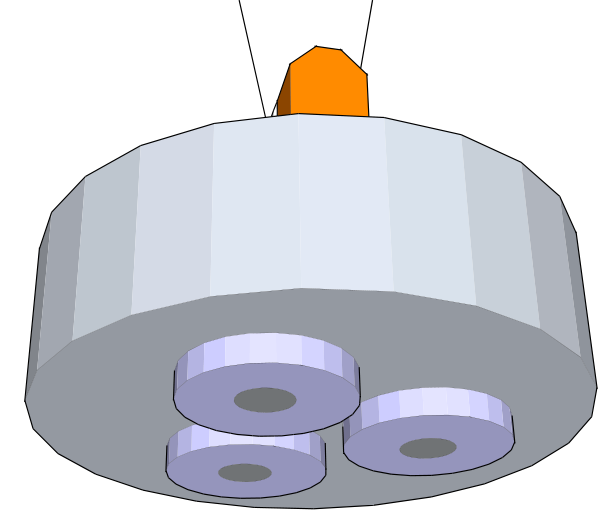
\includegraphics[width=0.3\textwidth]{Billeder/Electromagnet.png}
        \end{subfigure}

% \onslide<2-> \scalebox{0.8}{ \begin{subfigure}{0.98\textwidth}
%         \centering
%         \begin{tikzpicture}
%         \draw [fill = black, ultra thick] (-0.1,0) circle [radius=0.5];;
%         \draw [fill = black, ultra thick] (1.1,0) circle [radius=0.5];;
%         \draw [fill = black, ultra thick] (0.5,1) circle [radius=0.5];;

%         \draw [gray, ultra thick] (0.5,0.35) circle [radius=1.5];;


%         %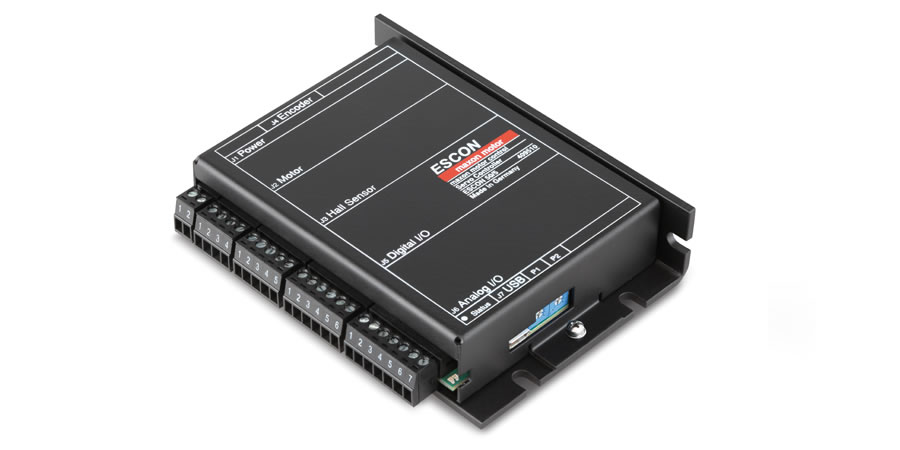
\includegraphics[width=0.5\textwidth]{Billeder/Escon_fig}
%         \end{tikzpicture}
%         \end{subfigure}
%         }

\vspace{0.45cm}
\onslide<3->  \begin{subfigure}{0.98\textwidth}
        \centering
        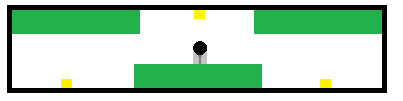
\includegraphics[width=0.5\textwidth]{Billeder/AngleSensor}
        \end{subfigure}     


\end{figure}

\end{column}
\end{columns}

\end{frame}



%%%%%%%%%%%%%%%%%%%%%%%%%%%%%%%%%%%%%%%%%%%%%%%%%%%%%%%%%%%%%%%%%%%%%%%%%%%%%%%%%%%

\begin{frame}{Optimering}{}


  \begin{itemize}
    \item<1-> Statisk friktion
  \end{itemize}

\vspace{0.5cm}
\centering
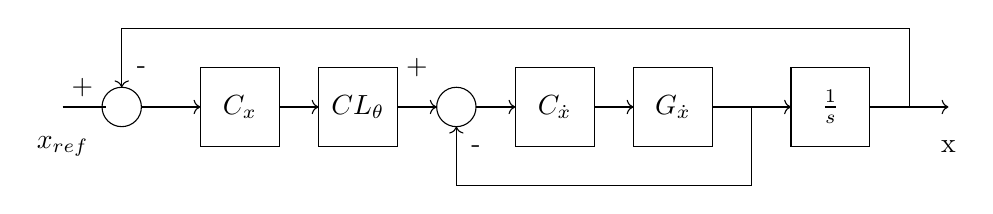
\begin{tikzpicture}

\draw  (-6,1.5) rectangle (-5,0.5);
\draw  (-4.5,1.5) rectangle (-3.5,0.5);
\draw  (-2,1.5) rectangle (-1,0.5);
\draw  (-0.5,1.5) rectangle (0.5,0.5);
\draw  (1.5,1.5) rectangle (2.5,0.5);
\draw  (-2.75,1) ellipse (0.25 and 0.25);
\draw  (-7,1) ellipse (0.25 and 0.25);
\draw (-7.75,1) -- (-7.2,1);

\draw [->](-6.75,1) -- (-6,1);

\draw [->](-5,1) -- (-4.5,1);

\draw [->](-3.5,1) -- (-3,1);

\draw [->](-2.5,1) -- (-2,1);

\draw [->](-1,1) -- (-0.5,1);

\draw [->](0.5,1) -- (1.5,1);

\draw [->](2.5,1) -- (3.5,1);

\draw [->](1,1) -- (1,0) -- (-2.75,0) -- (-2.75,0.75);

\draw [->](3,1) -- (3,2) -- (-7,2) -- (-7,1.25);

\node at (-5.5,1) {$C_x$};
\node at (-4,1) {$CL_\theta$};
\node at (-1.5,1) {$C_{\dot{x}}$};
\node at (0,1) {$G_{\dot{x}}$};
\node at (2,1) {$\frac{1}{s}$};
\node at (-7.5,1.25) {+};
\node at (-6.75,1.5) {-};
\node at (-3.25,1.5) {+};
\node at (-2.5,0.5) {-};
\node at (-7.75,0.5) {$x_{ref}$};
\node at (3.5,0.5) {x};
\end{tikzpicture}
 \end{frame}










%%%%%%%%%%




% \begin{frame}{Optimering}{}


%  \begin{minipage}[H]{0.3\linewidth}
%   \begin{itemize}
%     \item<1-> Static fiction
%   \end{itemize}
%   \end{minipage}

%   \vfill

%   \begin{center}
%   \scalebox{0.8}{
%   \begin{tikzpicture}
%   \draw  (-6,0.25) ellipse (0.25 and 0.25);
% \draw[->,thick] (-7.25,0.25) -- (-6.25,0.25);
% \draw  (-4.75,-0.25) rectangle (-2.75,0.75);
% \draw  (1.25,0.75) rectangle (3.25,-0.25);

% \node at (2.25,0.25) {$G_\dot{x}$};
% \draw  (4.25,0.75) rectangle (5.25,-0.25);
% \node at (4.75,0.25) {$\frac{1}{s}$};
% \draw[->,thick] (7.75,0.25) -- (7.75,1.75) -- (-6,1.75) -- (-6,0.5);
% \node at (6.5,0.25) {x};
% \draw[->,thick] (5.25,0.25) -- (6.25,0.25);

% %\draw  (7.25,0.75) rectangle (9.25,-0.25);

% \draw[->,thick] (-5.75,0.25) -- (-4.75,0.25);
% \draw[->,thick] (3.25,0.25) -- (4.25,0.25);



% \node at (-6.5,0.5) {+};
% \node at (-5.75,0.75) {-};
% \node at (-7.75,0.25) {x};

% \node at (-3.75,0.25) {$C_x$};

% \draw  (-1.75,-0.25) rectangle (0.25,0.75);
% \node at (-0.75,0.25) {$CL_\theta$};
% \draw[->,thick] (-2.75,0.25) -- (-1.75,0.25);
% \draw[->,thick] (0.25,0.25) -- (1.25,0.25);

% \end{tikzpicture}}
% \end{center}
%   \end{frame}




%%%%%%%%%%%%%%%%%%%%%%%%%%%%%%%%%%%%%%%%%%%%%%%%%%%%%%%%%%%%%%%%%%%%%%%%
\section{Konklusion}




\begin{frame}{Konklusion}{}
  \begin{itemize}
    \item<1-> Analyse af kran  
    \item<2-> Modeller er blevet udledt på baggrund af analyse  
    \item<3-> Parameter estimeringer 
    \item<4-> Root locus er benyttet under udvikling af regulatorer 
    \item<5-> Strøm offset kan kompensere for statisk friktion
    \item<6-> Kaskade kobling  
  \end{itemize}
\end{frame}




\begin{frame}{Demonstration}{Simon}
  \begin{itemize}
    \item<1-> Kontrol lab
  \end{itemize}
\end{frame}
%%%%%%%%%%%%%%%%

\end{document}
